\documentclass[color,DIV12,pdftex,a4paper]{ET-DS}
\usepackage{verbatim}
\usepackage[latin1]{inputenc}
\usepackage[T1]{fontenc}
%
\usepackage{ae}
\usepackage{lastpage}
\usepackage{amsmath,amssymb}
\usepackage{textcomp}
\usepackage{color}
\usepackage{colortbl}
\usepackage{parskip}
\usepackage{chapterbib}
\usepackage{xspace}
\usepackage[english]{babel}
\usepackage[pdftex]{graphicx}
\usepackage{float}
\usepackage[section]{placeins}
\usepackage[sectionbib, numbers, sort&compress, square]{natbib}
%\documentstyle{elsart-harv}
\usepackage[pdftex,pagebackref=true,pdfpagelabels=true]{hyperref}
\usepackage{framed} 
\usepackage{ifthen}

%%%%%%%%% begin: macros for creating  ET boxes %%%%%%%% 
\newcommand{\titlecolor}{white}
\newcommand{\captioncolor}{white}
\newcommand{\contentcolor}{white}
\newcommand{\ccolor}{\definecolor{citecolor}{rgb}{0,.5,0}}
\newcommand{\lcolor}{\definecolor{linkcolor}{rgb}{.8,0,0}}
\newcommand{\ucolor}{\definecolor{urlcolor}{rgb}{0,0,.7}}
\newcommand{\etboxwidth}{0.975\textwidth}
\newcommand{\etboxskip}{0.0125\textwidth} % this is (1-\etboxwidth)/2
\newcommand{\etboxmargin}{0.5cm}

\floatstyle{ruled} 
\newfloat{ETbox}{t}{lop}[section] %bhp

\newenvironment{ETboxenvironment}[1][\hsize]{%
\def\FrameCommand{\fcolorbox{framecolor}{shadecolor}}%
\MakeFramed{\hsize#1\advance\hsize-\width\FrameRestore}}%
{\endMakeFramed}

%%% The long ET box %%%%
\def\longetbox#1#2#3#4{ 
\definecolor{framecolor}{cmyk}{1,1,1,1}%
\ifthenelse{\equal{#1}{r}}{%
\definecolor{darkred}{rgb}{0.6,0,0}
\definecolor{semidarkred}{rgb}{0.8,0,0}
\floatname{ETbox}{\color{darkred}\large Box}% 
\renewcommand{\titlecolor}{darkred}%
\renewcommand{\captioncolor}{darkred}%
\renewcommand{\contentcolor}{semidarkred}%
\renewcommand{\ccolor}{\definecolor{citecolor}{rgb}{0,0,0.8}}%
\renewcommand{\lcolor}{\definecolor{linkcolor}{rgb}{.0,.8,0}}%
\renewcommand{\ucolor}{\definecolor{urlcolor}{rgb}{0,0.8,0.8}}%
\definecolor{shadecolor}{rgb}{1,0.9,0.7}}{%
\ifthenelse{\equal{#1}{i}}{%
\floatname{ETbox}{\color{blue}\large Box}% 
\renewcommand{\titlecolor}{blue}%
\renewcommand{\captioncolor}{blue}%
\renewcommand{\contentcolor}{blue}%
\renewcommand{\ccolor}{\definecolor{citecolor}{rgb}{0,.5,0}}
\renewcommand{\lcolor}{\definecolor{linkcolor}{rgb}{.8,0,0}}
\renewcommand{\ucolor}{\definecolor{urlcolor}{rgb}{0.9,0.,0.9}}
\definecolor{shadecolor}{cmyk}{.07,.01,0,0}}{%
\ifthenelse{\equal{#1}{h}}{%
\floatname{ETbox}{\color{blue}\large Box}% %%%%%%%%%%%%%%%%%%
\renewcommand{\titlecolor}{blue}%
\renewcommand{\captioncolor}{blue}%
\renewcommand{\contentcolor}{black}%
\renewcommand{\ccolor}{\definecolor{citecolor}{rgb}{0,.5,0}}%
\renewcommand{\lcolor}{\definecolor{linkcolor}{rgb}{.8,0,0}}%
\renewcommand{\ucolor}{\definecolor{urlcolor}{rgb}{0,0,.7}}%
\definecolor{shadecolor}{cmyk}{0,0,.3,0}}{}{}}}%
\vspace{\parskip} 
\color{\contentcolor}
\fboxrule 0.75pt
\setlength{\fboxsep}{\etboxmargin}
\begin{ETboxenvironment}[\etboxwidth] 
\arrayrulecolor{\contentcolor}
\ccolor
\lcolor
\ucolor
\captionsetup{labelfont={color=\contentcolor,bf}, textfont={color=\contentcolor}, labelsep=colon}%, margin=\etboxskip}%
\captionof{ETbox}[#3]{\textcolor{\captioncolor}{\large\bf#3}} 
\captionsetup{labelfont={color=\contentcolor,bf}, textfont={color=\contentcolor},labelsep=colon}%, margin=\etboxskip}  % add something of geometry
#4
\label{#2} 
\end{ETboxenvironment} 
\arrayrulecolor{black} 
\color{black} 
%\definecolor{citecolor}{rgb}{0,.5,0}
%\definecolor{linkcolor}{rgb}{.8,0,0}
%\definecolor{urlcolor}{rgb}{0,0,.7}

}
%%%%%%%%%%  %%%%%%%%


%%%%%%% the one-page ETbox %%%%%%%% 

\def\etbox#1#2#3#4{ 
\definecolor{framecolor}{cmyk}{1,1,1,1}%
\ifthenelse{\equal{#1}{r}}{%
\definecolor{darkred}{rgb}{0.6,0,0}
\definecolor{semidarkred}{rgb}{0.8,0,0}
\floatname{ETbox}{\color{darkred}\large Box}% 
\renewcommand{\titlecolor}{darkred}%
\renewcommand{\captioncolor}{darkred}%
\renewcommand{\contentcolor}{semidarkred}%
\renewcommand{\ccolor}{\definecolor{citecolor}{rgb}{0,0,0.8}}%
\renewcommand{\lcolor}{\definecolor{linkcolor}{rgb}{.0,.8,0}}%
\renewcommand{\ucolor}{\definecolor{urlcolor}{rgb}{0,0.8,0.8}}%
%\floatname{ETbox}{\color{white}\large Box}% 
%\renewcommand{\titlecolor}{white}%
%\renewcommand{\captioncolor}{white}%
%\renewcommand{\contentcolor}{white}%
%\renewcommand{\ccolor}{\definecolor{citecolor}{rgb}{.4,.9,.9}}%
%\renewcommand{\lcolor}{\definecolor{linkcolor}{rgb}{.9,.9,0}}%
%\renewcommand{\ucolor}{\definecolor{urlcolor}{rgb}{0,0.9,.5}}%
%\definecolor{shadecolor}{cmyk}{.0,.8,.7,0}}{%
\definecolor{shadecolor}{rgb}{1,0.9,0.7}}{%
%\definecolor{shadecolor}{rgb}{0.65,0.09,0.09}}{%
\ifthenelse{\equal{#1}{i}}{%
\floatname{ETbox}{\color{blue}\large Box}% 
\renewcommand{\titlecolor}{blue}%
\renewcommand{\captioncolor}{blue}%
\renewcommand{\contentcolor}{blue}%
\renewcommand{\ccolor}{\definecolor{citecolor}{rgb}{0,.5,0}}
\renewcommand{\lcolor}{\definecolor{linkcolor}{rgb}{.8,0,0}}
\renewcommand{\ucolor}{\definecolor{urlcolor}{rgb}{0.9,0.,0.9}}
\definecolor{shadecolor}{cmyk}{.07,.01,0,0}}{%
\ifthenelse{\equal{#1}{h}}{%
\floatname{ETbox}{\color{blue}\large Box}% 
\renewcommand{\titlecolor}{blue}%
\renewcommand{\captioncolor}{blue}%
\renewcommand{\contentcolor}{black}%
\renewcommand{\ccolor}{\definecolor{citecolor}{rgb}{0,.5,0}}%
\renewcommand{\lcolor}{\definecolor{linkcolor}{rgb}{.8,0,0}}%
\renewcommand{\ucolor}{\definecolor{urlcolor}{rgb}{0,0,.7}}%
\definecolor{shadecolor}{cmyk}{0,0,.3,0}}{}{}}}%
\begingroup
\begin{center}   
\begin{minipage}[t]{\etboxwidth} 
\leftskip=\etboxskip
\rightskip=\etboxskip
\definecolor{framecolor}{cmyk}{1,1,1,1}
\begin{framed} 
\vspace{-9pt} 
\arrayrulecolor{\contentcolor}
\begin{shaded}       
\lcolor
\ccolor
\ucolor
\captionsetup{labelfont={color=\captioncolor,bf}, textfont={color=\captioncolor}, labelsep=colon, margin=\etboxskip}%
\captionof{ETbox}[#3]{\textcolor{\captioncolor}{\large\bf#3}} 
\captionsetup{labelfont={color=\titlecolor,bf}, textfont={color=\contentcolor},labelsep=colon, margin=\etboxskip}%\etboxmargin} 
\textcolor{\contentcolor}{#4} 
\label{#2} 
\end{shaded} 
\vspace{-9pt} 
\end{framed} 
\end{minipage} 
\end{center} 
\endgroup
\vspace{9pt} 
\arrayrulecolor{black} 
\color{black} 
%\definecolor{citecolor}{rgb}{0,.5,0}
%\definecolor{linkcolor}{rgb}{.8,0,0}
%\definecolor{urlcolor}{rgb}{0,0,.7}
}
%%%%%%%%%%% end: macros for creating a box %%%%%%%%
%





%%% begin:  macros for creating the Glossary %%%%%%%
\usepackage{ifthen}
\usepackage[cfg, intoc]{nomencl}
\renewcommand{\nomgroup}[1]{%
 \ifthenelse{\equal{#1}{S}}{\vspace{30pt}\item[]\hspace*{-\leftmargin}%
 \rule[2pt]{0.45\linewidth}{1pt}%
 \hfill \textbf{Symbols} \hfill
 \rule[2pt]{0.45\linewidth}{1pt}\vspace{-5pt} \item[]\hspace*{-\leftmargin}\vspace{5pt}\hspace{1.1cm}Please note that some symbols might stand for more than one quantity depending on the context}{%
\ifthenelse{\equal{#1}{A}}{\item[]\hspace*{-\leftmargin}
\rule[2pt]{0.45\linewidth}{1pt}%
\hfill \textbf{Abbreviations} \hfill
\rule[2pt]{0.45\linewidth}{1pt}}{%
\ifthenelse{\equal{#1}{G}}{\vspace{30pt}\item[]\hspace*{-\leftmargin}
\rule[2pt]{0.45\linewidth}{1pt}%
\hfill \textbf{Glossary} \hfill
\rule[2pt]{0.45\linewidth}{1pt}}{}{}}}}
\renewcommand{\nomname}{Nomenclature}
\makenomenclature
       %%% end:  macros for creating the  Glossary %%%%%%%


\definecolor{linkcolor}{rgb}{.8,0,0}
\definecolor{urlcolor}{rgb}{0,0,.7}
\definecolor{citecolor}{rgb}{0,.5,0}
\definecolor{acrocolor}{rgb}{0,0,.7}
\hypersetup{bookmarksopen,colorlinks=true}
\hypersetup{pdfstartview=FitH}
\hypersetup{linktocpage=true,bookmarksnumbered=true}
\hypersetup{plainpages=false,breaklinks=true}
\hypersetup{linkcolor=linkcolor,citecolor=citecolor,urlcolor=urlcolor}
%\usepackage{float}
\usepackage{tabularx}
\usepackage{longtable}
\usepackage{colortbl}
\usepackage{hhline}
\usepackage{multirow}
\usepackage{subfigure}
\usepackage{eurosym}
\usepackage{rotating}
\usepackage[absolute]{textpos}
\usepackage[page,toc]{appendix}
\usepackage{wrapfig}



%
% comment this line to cancel the watermark

%\usepackage{everypage,draftwatermark}
%\pdfminorversion=6
%
% separates the caption from the text and make the caption label bold: 
%
\usepackage[hang,small,bf]{caption}
%
% user defined commands
%
% \citeurl{key} cite the URL of a web site, if this has been inserted in the .bbl file as author of a (electronic) entry
%
\newcommand{\citeurl}[1]
{
\citeauthor{#1}\@\xspace
}
%
% \citeurlp is like \citeurl, but between parentesis
%
\newcommand{\citeurlp}[1]
{
(\citeauthor{#1})\@\xspace
}
\newcommand{\beq}{\begin{equation}}
\newcommand{\eeq}{\end{equation}}
\newcommand{\bear}{\begin{array}}
\newcommand{\ear}{\end{array}}
\newcommand{\dy}{\displaystyle}
\newcommand{\beg}{\begin{gathered}}
\newcommand{\eeg}{\end{gathered}}
%pdf stuff
\pdfinfo{/Title ET Design Study document
        /Subject Einstein Telescope
         /Author (ET Science Team)
         /Keywords (gravitational wave  Einstein Telescope design study)}
\pagenumbering{roman}

\title{Einstein gravitational wave Telescope conceptual design study} \shorttitle{ET Design Study}
\refnum{ET-0106C-10}
\issue{4}
%\documentclass[12pt]{iopart}
%\begin{document}
%\author{CQC author list, to be changed with the DS author list,}
\author{M\,Abernathy$^{1}$,
F\,Acernese$^{2,3}$,
P\,Ajith$^{30}$,
B\,Allen$^{4}$,
P\,Amaro-Seoane$^{54,32}$,
N\,Andersson$^{5}$,\and
S\,Aoudia$^{54}$,  
P\,Astone$^{6,7}$, 
B\,Krishnan$^{4}$,
L\,Barack$^{5}$,
F\,Barone$^{2,3}$,
B\,Barr$^{1}$,
M\,Barsuglia$^{8}$,\and
M\,Bassan$^{9,10}$,
R\,Bassiri$^{1}$, 
M\,Beker$^{11}$, 
N\,Beveridge$^{1}$,
M\,Bizouard$^{12}$, 
C\,Bond$^{13}$,
S\,Bose$^{14}$,\and
L\,Bosi$^{15}$,
S\,Braccini$^{16}$,
C\,Bradaschia$^{16,17}$,  
M\,Britzger$^{4}$,
F\,Brueckner$^{18}$,
T\,Bulik$^{19}$,\and
H\,J\,Bulten$^{20}$,
O\,Burmeister$^{4}$, 
E\,Calloni$^{2,21}$,
P\,Campsie$^{1}$,
L\,Carbone$^{13}$,
G\,Cella$^{16}$,\and
E\,Chalkley$^{13}$, 
E\,Chassande-Mottin$^{8}$, 
S\,Chelkowski$^{13}$,
A\,Chincarini$^{22}$, 
A\,Di\,Cintio$^{6}$,
J\,Clark$^{26}$,\and
E\,Coccia$^{9,10}$,
C\,N\,Colacino$^{16}$,
J\,Colas$^{17}$,
A\,Colla$^{6,7}$,
A\,Corsi$^{30}$,  
A\,Cumming$^{1}$,  
L\,Cunningham$^{1}$,\and
E\,Cuoco$^{17}$,
S\,Danilishin$^{23}$,
K\,Danzmann$^{4}$, 
E\,Daw$^{28}$,
R\,De\,Salvo$^{25}$,  
W\,Del\,Pozzo$^{11}$,\and
T\,Dent$^{26}$,
R\,De\,Rosa$^{2,21}$,
L\,Di\,Fiore$^{2}$, 
M\,Di\,Paolo\,Emilio$^{9}$,
A\,Di\,Virgilio$^{16}$,  
A\,Dietz$^{27}$,\and 
M\,Doets$^{11}$,
J\,Dueck$^{4}$,
M\,Edwards$^{26}$, 
V\,Fafone$^{9,10}$
S\,Fairhurst$^{26}$,  
P\,Falferi$^{29,56}$,\and
M\,Favata$^{30}$,
V\,Ferrari$^{6,7}$, 
F\,Ferrini$^{17}$, 
F\,Fidecaro$^{17,51}$,
R\,Flaminio$^{31}$,
J\,Franc$^{31}$, \and
F\,Frasconi$^{16}$, 
A\,Freise$^{13}$,
D\,Friedrich$^{4}$,
P\,Fulda$^{13}$,  
J\,Gair$^{57}$,
M\,Galimberti$^{31}$,
G\,Gemme$^{22}$,
E\,Genin$^{17}$, \and
A\,Gennai$^{16}$,
A\,Giazotto$^{16,17}$,
K\,Glampedakis$^{40}$,
R\,Gouaty$^{27}$,
C\,Graef$^{4}$,
W\,Graham$^{1}$,
M\,Granata$^{8}$, \and
H\,Grote$^{4}$, 
G\,Guidi$^{33,34}$, 
J\,Hallam$^{13}$,
G\,Hammond$^{1}$,
M\,Hannam$^{26}$,
J\,Harms$^{30}$,  
K\,Haughian$^{1}$,\and
I\,Hawke$^{5}$, 
D\,Heinert$^{18}$,  
M\,Hendry$^{1}$,
I\,Heng$^{1}$,
E\,Hennes$^{11}$, 
S\,Hild$^{1}$,
J\,Hough$^{1}$,
D\,Huet$^{17}$,
S\,Husa$^{55}$,\and
S\,Huttner$^{1}$,  
B\,Iyer$^{38}$,
D\,I\,Jones$^{5}$,
G\,Jones$^{1}$,
I\,Kamaretsos$^{26}$, 
C\,Kant Mishra$^{38}$,
F\,Kawazoe$^{4}$,  \and 
F\,Khalili$^{39}$, 
B\,Kley$^{18}$,
K\,Kokeyama$^{13}$,
K\,Kokkotas$^{40}$,
S\,Kroker$^{18}$,
R\,Kumar$^{1}$,  \and
K\,Kuroda$^{41}$, 
B\,Lagrange$^{31}$,
N\,Lastzka$^{4}$,
T\,G\,F\,Li$^{11}$,
M\,Lorenzini$^{33}$,
G\,Losurdo$^{33,17}$,
H\,L\"{u}ck$^{4}$,  \and
E\,Majorana$^{6}$,
V\,Malvezzi$^{9,10}$,  
I\,Mandel$^{42,13}$, 
V\,Mandic$^{36}$,
S\,Marka$^{50}$,
F\,Marin$^{33}$,  
F\,Marion$^{27}$,\and
J\,Marque$^{17}$,
I\,Martin$^{1}$, 
D\,Mc\,Leod$^{26}$,
D\,Mckechan$^{26}$, 
M\,Mehmet$^{4}$, 
C\,Michel$^{31}$,\and
Y\,Minenkov$^{9}$,  
N\,Morgado$^{31}$,
A\,Morgia$^{9}$,
S\,Mosca$^{2,21}$
L\,Moscatelli$^{6}$,
B\,Mours$^{27}$, \and
H\,M\"{u}ller-Ebhardt$^{4}$,
P\,Murray$^{1}$, 
L\,Naticchioni$^{6,7}$,
R\,Nawrodt$^{18}$,
J\,Nelson$^{1}$,
R\,O'\,Shaughnessy$^{43}$, \and
C\,D\,Ott$^{30}$,  
C\,Palomba$^{6}$, 
A\,Paoli$^{17}$,
G\,Parguez$^{17}$,  
A\,Pasqualetti$^{17}$,\and
R\,Passaquieti$^{16}$,
D\,Passuello$^{16}$,  
M\,Perciballi$^{6}$,  
F\,Piergiovanni$^{33,34}$, \and
L\,Pinard$^{31}$,
M\,Pitkin$^{1}$,
W\,Plastino$^{44}$,
M\,Plissi$^{1}$,
R\,Poggiani$^{16}$, 
P\,Popolizio$^{17}$,  
E\,Porter$^{8}$,\and
M\,Prato$^{22}$, 
G\,Prodi$^{45,56}$, 
M\,Punturo$^{15,17}$,
P\,Puppo$^{6}$,
D\,Rabeling$^{20}$,
I\,Racz$^{46}$,
P\,Rapagnani$^{6,7}$,\and  
V\,Re$^{9}$,
J\,Read$^{37}$,
T\,Regimbau$^{47}$,
H\,Rehbein$^{4}$,
S\,Reid$^{1}$,
L\,Rezzolla$^{54}$,\and
F\,Ricci$^{6,7}$,  
F\,Richard$^{17}$,
A\,Rocchi$^{9}$,
R\,Romano$^{2}$,
S\,Rowan$^{1}$,
A\,R\"{u}diger$^{4}$, \and
A\,Samblowski$^{4}$, 
L\,Santamar{\'i}a$^{30}$,
B\,Sassolas$^{31}$,
B\,Sathyaprakash$^{26}$,
R\,Schilling$^{4}$,\and
P\,Schmidt$^{26}$,  
R\,Schnabel$^{4}$,
B\,Schutz$^{26,54}$,
C\,Schwarz$^{18}$,
J\,Scott$^{1}$,
P\,Seidel$^{18}$,
A\,M\,Sintes$^{55}$, \and
K\,Somiya$^{48}$,  
C\,F\,Sopuerta$^{49}$,
B\,Sorazu$^{1}$,
F\,Speirits$^{1}$,
L\,Storchi$^{15}$,
K\,Strain$^{1}$,
S\,Strigin$^{23}$,
P\,Sutton$^{26}$,\and  
S\,Tarabrin$^{4}$,
B\,Taylor$^{4}$,
A\,Th\"{u}rin$^{4}$,
K\,Tokmakov$^{1}$,
M\,Tonelli$^{16,51}$, 
H\,Tournefier$^{27}$,\and
R\,Vaccarone$^{17}$,
H\,Vahlbruch$^{4}$, 
J\,F\,J\,van\,den\,Brand$^{11,20}$,
C\,Van\,Den\,Broeck$^{11}$, 
S\,van\,der\,Putten$^{11}$,\and
M\,van\,Veggel$^{1}$,
A\,Vecchio$^{13}$, 
J\,Veitch$^{26}$,
F\,Vetrano$^{33,34}$,
A\,Vicere$^{33,34}$, 
S\,Vyatchanin$^{23}$, \and 
P\,We{\ss}els$^{52}$,
B\,Willke$^{4}$,
W\,Winkler$^{4}$, 
G\,Woan$^{1}$,
K\,Wojcik$^{26}$,
A\,Woodcraft$^{53}$,
K\,Yamamoto$^{35}$
}
\affiliation{
{$^{1}$\,Department of Physics and Astronomy, The University of Glasgow, Glasgow, G12\,8QQ, UK}
\\{$^{2}$\,INFN, Sezione di Napoli, Italy}
\\{$^{3}$\,Universit\`{a} di Salerno, Fisciano, I-84084 Salerno, Italy}
\\{$^{4}$\,Max--Planck--Institut f\"{u}r Gravitationsphysik und Leibniz Universit\"{a}t Hannover, D-30167 Hannover, Germany}
\\{$^{5}$\,University of Southampton, Southampton SO17\,1BJ, UK}
\\{$^{6}$\,INFN, Sezione di Roma 1, I-00185 Roma, Italy}
\\{$^{7}$\,Universit\`{a} \textquoteleft La Sapienza\textquoteright, I-00185 Roma, Italy}
\\{$^{8}$\,Laboratoire AstroParticule et Cosmologie (APC), Universit\`{e} Paris Diderot, CNRS: IN2P3, CEA:DSM/IRFU, Observatoire de Paris, 10 rue A.Domon et L.Duquet, 75013 Paris - France}
\\{$^{9}$\,INFN, Sezione di Roma Tor Vergata I-00133 Roma, Italy}
\\{$^{10}$\,Universit\`{a} di Roma Tor Vergata, I-00133, Roma, Italy}
\\{$^{11}$\,Nikhef, Science Park, Amsterdam, the Netherlands}
\\{$^{12}$\,LAL, Universit\'{e} Paris-Sud, IN2P3/CNRS, F-91898 Orsay, France}
\\{$^{13}$\,University of Birmingham, Birmingham, B15 2TT, UK}
\\{$^{14}$\,Washington State University, Pullman, WA 99164, USA}
\\{$^{15}$\,INFN, Sezione di Perugia, Italy} 
\\{$^{16}$\,INFN, Sezione di Pisa, Italy}
\\{$^{17}$\,European Gravitational Observatory (EGO), I-56021 Cascina (Pi), Italy}
\\{$^{18}$\,Friedrich--Schiller--Universit\"{a}t Jena PF 07737 Jena, Germany}
\\{$^{19}$\,Astronomical Observatory, University of Warsaw, 00-478, Warszawa, Poland}
\\{$^{20}$\,VU University Amsterdam, De Boelelaan 1081, 1081 HV, Amsterdam, The Netherlands}
\\{$^{21}$\,Universit\`{a} di Napoli \textquoteleft Federico II\textquoteright, Complesso Universitario di Monte S. Angelo, I-80126 Napoli, Italy}
\\{$^{22}$\,INFN, Sezione di Genova, I-16146 Genova, Italy}
\\{$^{23}$\,Moscow State University, Moscow, 119992, Russia}
\\{$^{24}$\,INFN, Laboratori Nazionali del Gran Sasso, Assergi l'Aquila, Italy}
\\{$^{25}$\,Universit\`{a} degli Studi del Sannio, Benevento, Italy}
\\{$^{26}$\,Cardiff University, Cardiff, CF24 3AA, UK}
\\{$^{27}$\,LAPP-IN2P3/CNRS, Universit\'{e} de Savoie, F-74941 Annecy-le-Vieux, France}
\\{$^{28}$\,University of Sheffield, UK}
\\{$^{29}$\,Istituto di Fotonica e Nanotecnologie, CNR-Fondazione Bruno Kessler, 38123 Povo, Trento, Italy}
\\{$^{30}$\,Caltech--CaRT, Pasadena, CA 91125, USA}
\\{$^{31}$\,Laboratoire des Mat\'{e}riaux Avanc\'{e}s (LMA), IN2P3/CNRS, F-69622 Villeurbanne, Lyon, France}
\\{$^{32}$\,Institut de Ci{\`e}ncies de l'Espai, Campus UAB, Torre C-5, parells, 2na plantaES-08193 Bellaterra (Barcelona) }
\\{$^{33}$\,INFN, Sezione di Firenze, I-50019 Sesto Fiorentino, Italy}
\\{$^{34}$\,Universit\`{a} degli Studi di Urbino \textquoteleft Carlo Bo\textquoteright, I-61029 Urbino, Italy}
\\{$^{35}$\,INFN, Sezione di Padova, Italy}
\\{$^{36}$\,University of Minnesota, Minneapolis, MN 55455, USA}
\\{$^{37}$\,Department of Physics and Astronomy, University of Mississippi, Oxford, US}
\\{$^{38}$\,Raman research institute, Bangalore, India}
\\{$^{39}$\,Moscow State University, Moscow, 119992, Russia}
\\{$^{40}$\,Theoretical Astrophysics (TAT) Eberhard-Karls-Universit\"at T\"ubingen, Auf der Morgenstelle 10, D-72076 T\"{u}bingen, Germany}
\\{$^{41}$\,Institute for Cosmic Ray Research, University of Tokyo, Kashiwa, Chiba, Japan}
\\{$^{42}$\,MIT Kavli Institute, Cambridge, MA 02139, US}
\\{$^{43}$\,The Pennsylvania State University, University Park, PA 16802, USA}
\\{$^{44}$\,INFN, Sezione di Roma Tre and Universit\`{a} di Roma Tre-Dipartimento di Fisica, I-00146 Roma, Italy}
\\{$^{45}$\,Universit\`{a} di Trento, Trento, Italy}
\\{$^{46}$\,KFKI Research Institute for Particle and Nuclear Physics, Budapest, Hungary}
\\{$^{47}$\,Universit\'{e} Nice \textquoteleft Sophia--Antipolis\textquoteright, CNRS, Observatoire de la C\^ote d'Azur, F-06304 Nice, France}
\\{$^{48}$\,Department of Physics, Tokyo Institute of Technology, Tokyo, Japan}
\\{$^{49}$\,Institute of Space Sciences (CSIC-IEEC), Campus UAB, 08193 Bellaterra, Barcelona, Spain}
\\{$^{50}$\,Department of Physics, Columbia University, New York, US}
\\{$^{51}$\,Dipartimento di Fisica, Universit\`{a} di Pisa, Pisa, Italy}
\\{$^{52}$\,Laser Zentrum Hannover e.V., Hollerithallee 8, D-30419 Hannover, Germany}
\\{$^{53}$\,Royal Observatory, Blackheath Avenue, Greenwich, SE10 8XJ, UK}
\\{$^{54}$\,Max--Planck--Institut f\"{u}r Gravitationsphysik, D-14476 Potsdam, Germany}
\\{$^{55}$\,Departament de Fisica, Universitat de les Illes Balears, Cra. 
Valldemossa Km. 7.5, E-07122 Palma de Mallorca, Spain}
\\{$^{56}$\,INFN, Gruppo Collegato di Trento, Italy}
\\{$^{57}$\,Institute of Astronomy, University of Cambridge, Cambridge, CB3 0HA, UK}
}

%\end{document}

%
\date{\today}

\begin{document}
\begin{textblock*}{300mm}(0mm,0mm)   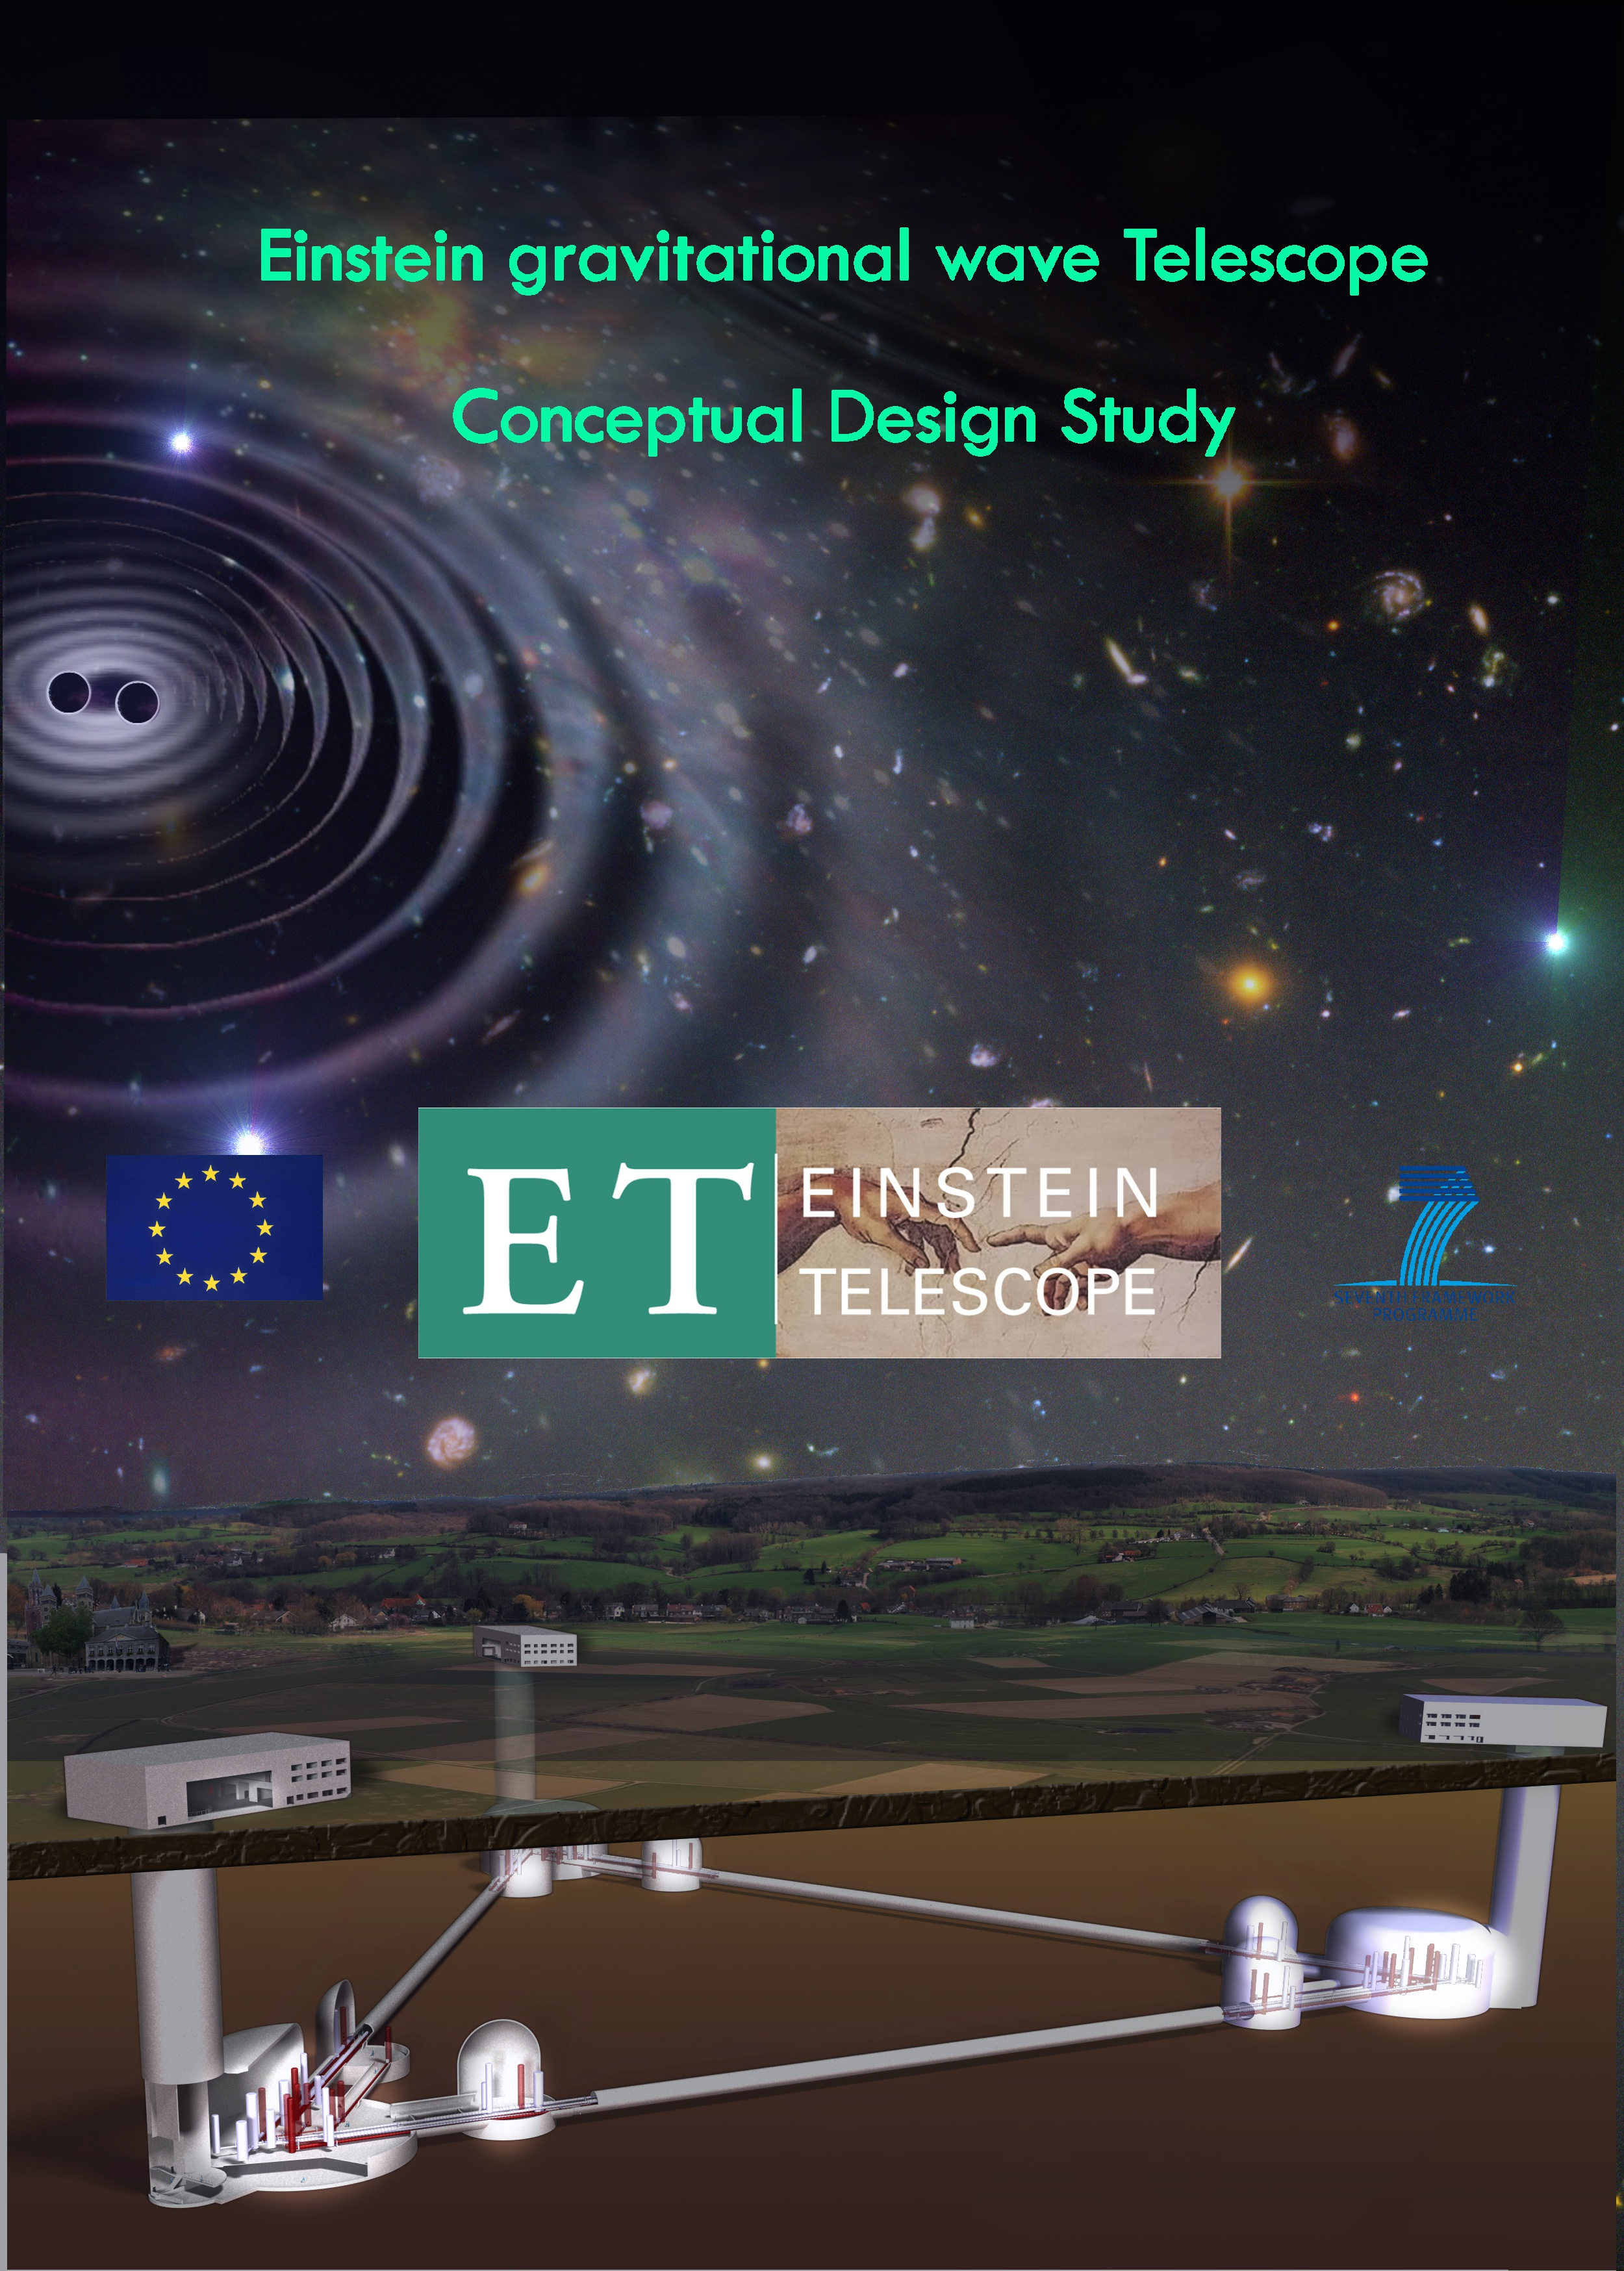
\includegraphics[width=\paperwidth]{Sec_Conclusions/FirstPagelatest4.jpg}
\end{textblock*}
%
%\newpage
%\cleardoublepage 
%\SetWatermarkText{Confidential}
%
\selectlanguage{english}
\begin{titlepage}
\pdfbookmark[1]{Title}{title}
\maketitle
\end{titlepage}
\clearpage
%
\FloatBarrier
%
\section*{Abstract}
% write here a short abstract, 10 line max
This document describes the Conceptual Design of a third generation gravitational wave observatory named Einstein Telescope (``ET''). The design of this new research infrastructure has been realised with the support of the European Community's Seventh Framework
Programme (FP7/2007-2013) under grant agreement n~211743.  In this document are described the fundamental design options, the site requirements, the main technological solutions, a rough evaluation of the costs and a schematic time plan.
%
\vspace{1cm}

\pagenumbering{arabic}
\setcounter{page}{4}
%
{\setlength{\baselineskip}{0pt} \tableofcontents}
\vspace{1cm}
\hrule height 1pt
%\vspace{1cm}


\citeindextrue
\cleardoublepage  
%\FloatBarrier
%\newpage
%\begin{textblock*}{297mm}(-2mm,1mm)   
%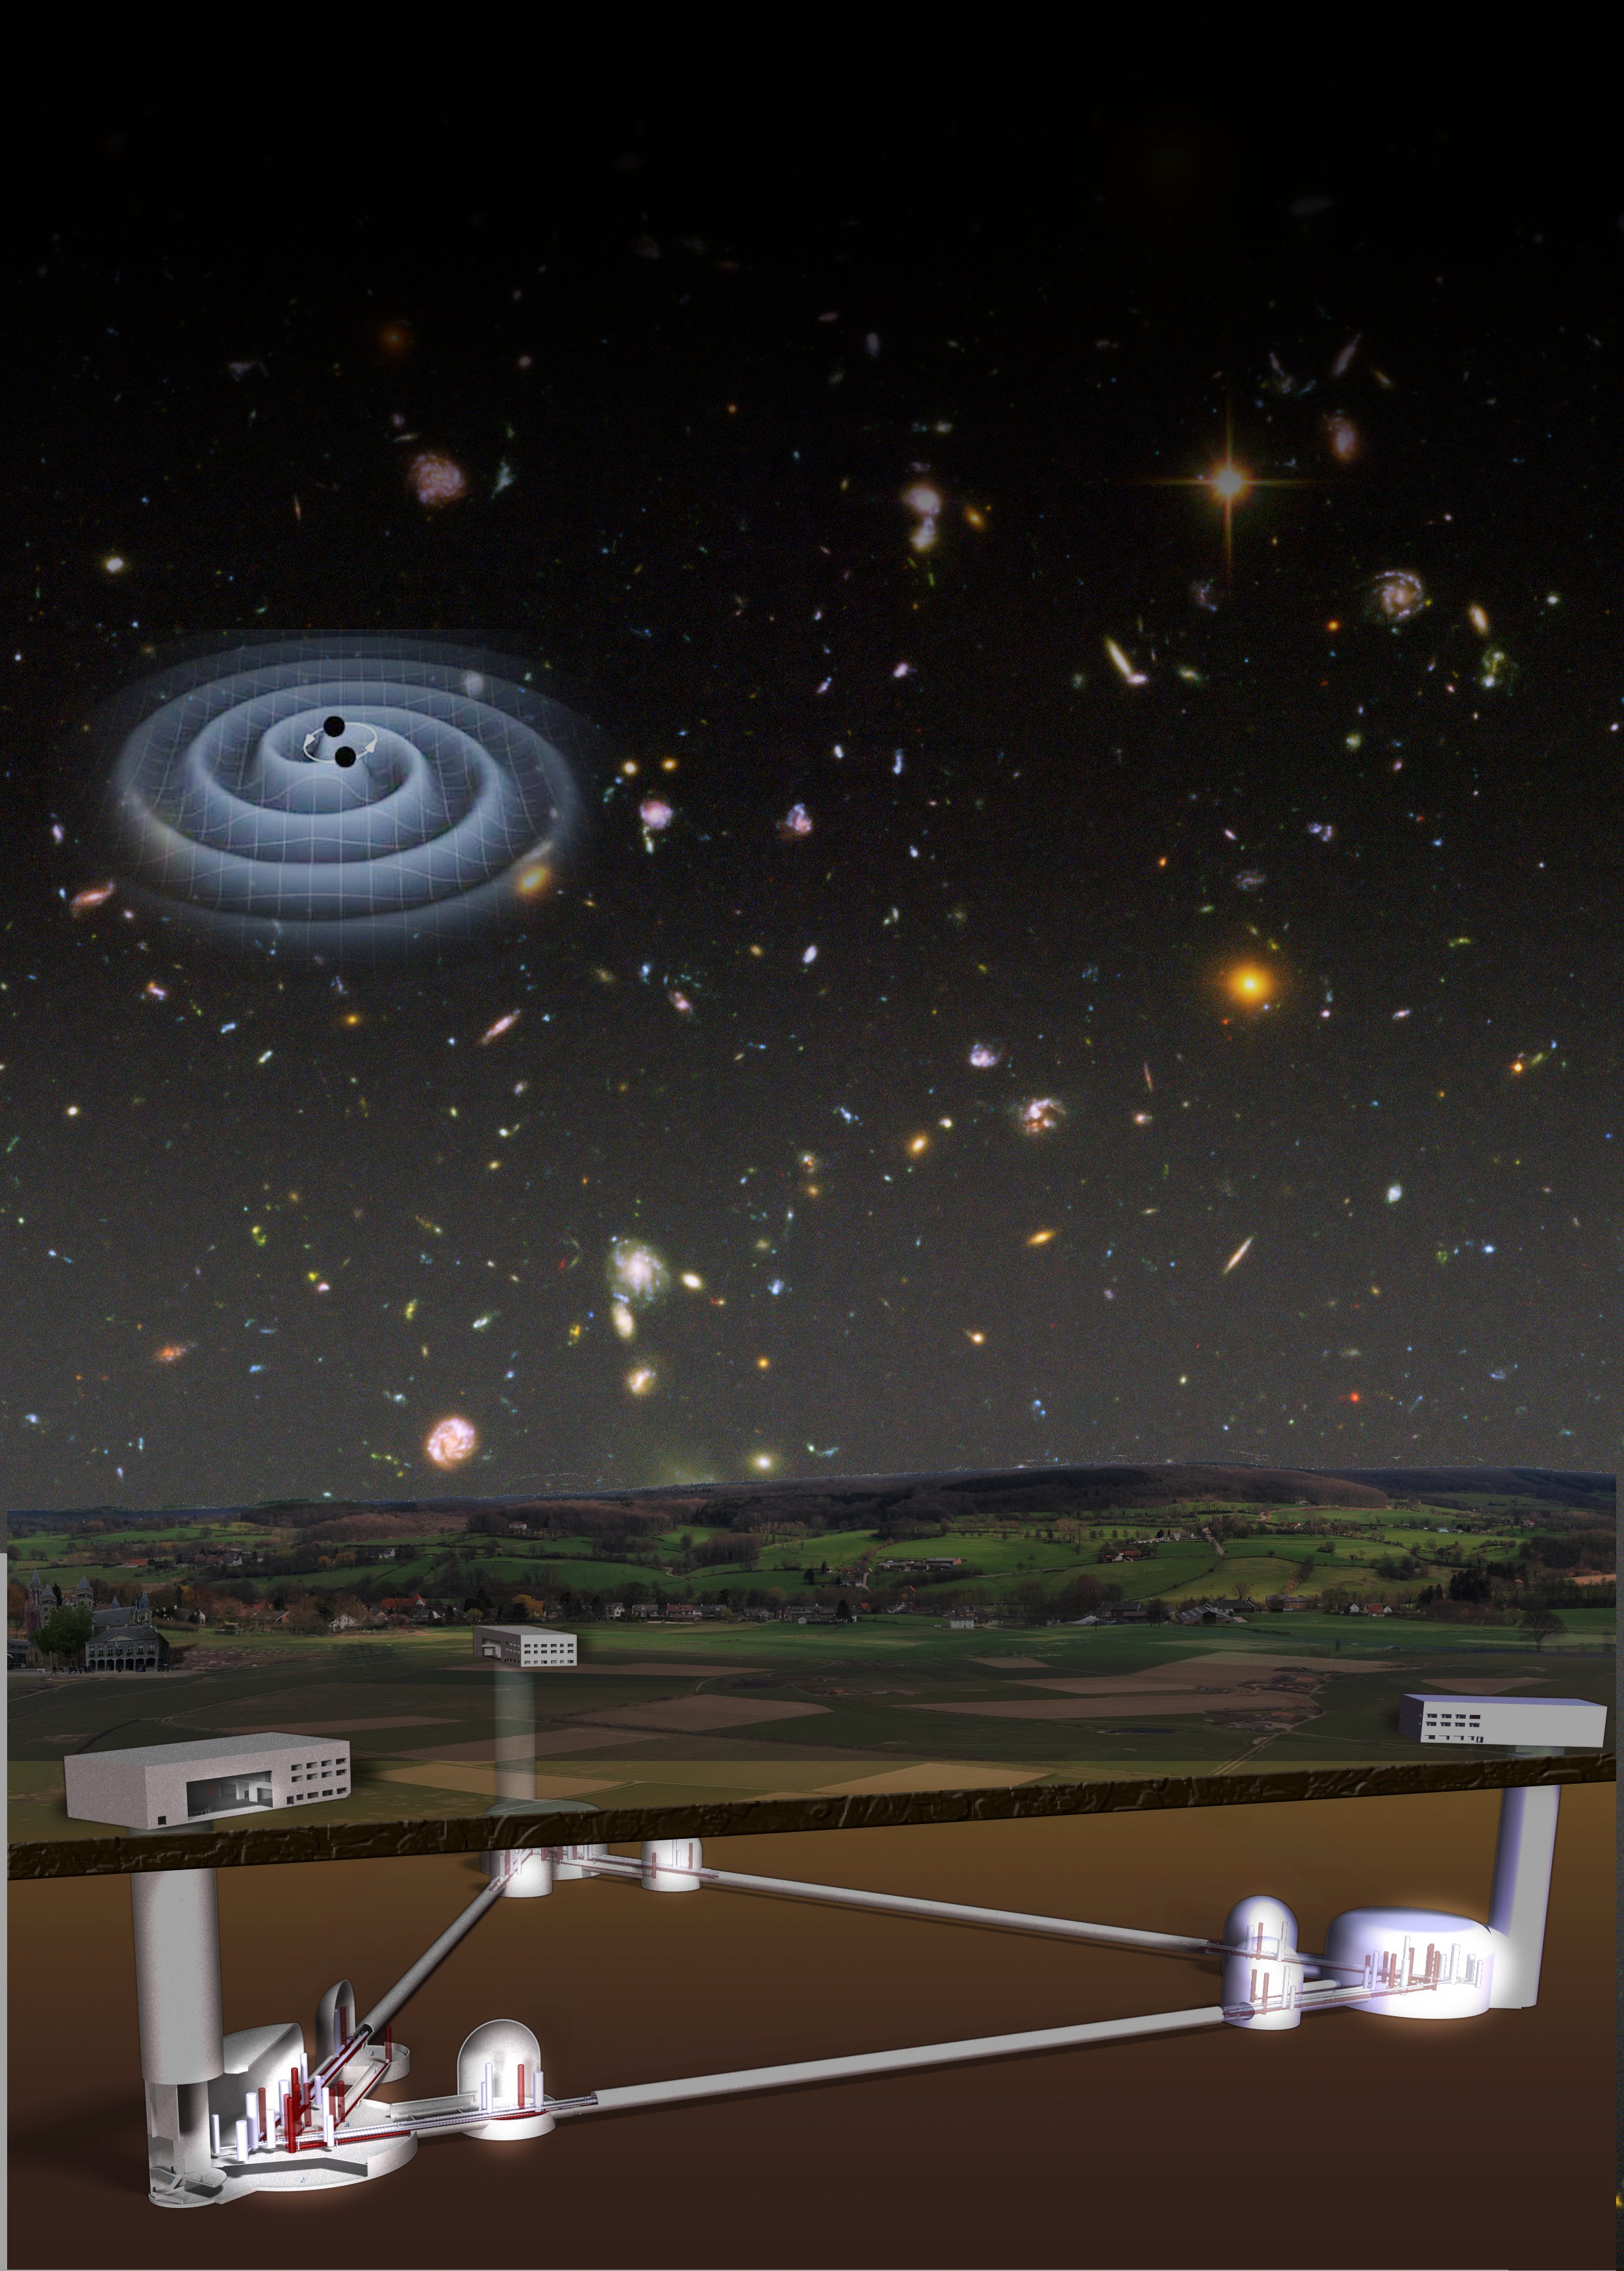
\includegraphics[width=1.01\paperwidth]{ETatNight.jpg}
%\end{textblock*}
%\begin{center}
%\Huge \textcolor{yellow}{The Einstein gravitational wave Telescope \\Design Study}
%\end{center}
%\normalsize
\cleardoublepage  
\FloatBarrier
\section{Introduction to the ET project}

%
% Extensive description of the document; history, table of the acronyms
%
% Author:
% Version:
%
\subsection[Prologue]{Prologue}
\label{Prologue}
The first generation of interferometric gravitational wave (GW) detectors 
(GEO600~\cite{GEO600Grote2008}, LIGO~\cite{Abbott2009}, 
TAMA~\cite{Arai2008}, Virgo~\cite{VirgoStatus2008}) have reached or 
approached their design sensitivities, and thus demonstrated the 
effectiveness of the working principle. The major detectors currently 
operative are enhanced versions of the first generation (Virgo+ and eLIGO), 
with higher laser power and some technological improvements. \par
Advanced detectors (like ``Advanced LIGO"\,(\cite{AdvancedLIGOReference2009},\,\cite{aLIGO}) and ``Advanced Virgo" \,(\cite{AdV2009})), also 
called the second generation, will show a sensitivity improved roughly by 
a factor of ten with respect to the initial interferometers. They are based on 
technologies currently available, sometimes tested in reduced scale 
prototypes, but still to be implemented in full scale. According to the current 
models of GW sources, the sensitivity of the advanced interferometers is 
expected to guarantee the detection of signals generated by astrophysical 
sources within months to a year at most. For example, at the nominal sensitivity 
of the advanced detectors, the expected detection rate of the GW signal 
generated by a binary system of coalescing neutron stars is about a few tens 
per year. But apart from extremely rare events, the expected signal-to-noise 
ratio (SNR) of these detections obtained with the advanced detectors is too low 
for precise astronomical studies of the GW sources and for complementing 
optical and X--ray observations in the study of fundamental systems and 
processes in the Universe. \par
These considerations led the GW community to start investigating a new (third) 
generation of detectors. In particular, the European Commission supported the 
institutions in Table~\ref{table:Beneficiaries} to realise this design study within 
the Seventh Framework Programme (FP7-Capacities). With a considerably 
improved sensitivity, such new machines of the third-generation will open the 
era of routine GW astronomy and with the Einstein Telescope (ET) project 
Europe will lead this scientific revolution. Since the first detection of a GW 
signal is expected to occur in the advanced interferometers, the evaluation 
of the scientific impact of ET it is especially focused on the observational aspects 
rather than on the detection capabilities. \par
To realise a third-generation GW observatory with a significantly enhanced 
sensitivity (we defined a target of a factor of ten improvement in sensitivity for 
ET with respect to the advanced detectors over a wide frequency range), several 
limitations of the technologies adopted in the advanced interferometers must 
be overcome and new solutions to be developed are proposed in this document 
to reduce the fundamental and technical noises that will limit the next generation 
machines. \par
%

\begin{table}[b]
% For LaTeX tables use
\centering
\caption{Institutions participating (``Beneficiaries") to the ET design study.}
\label{table:Beneficiaries}       % Give a unique label
\begin{tabular}{c|c}
\hline
\hline
Institute & Country   \\
\hline \hline
European Gravitational Observatory & Italy--France \\
\hline
Istituto Nazionale di Fisica Nucleare & Italy \\
\hline
Max-Planck-Gesellschaft zur F{\" o}rderung der Wissenschaften e.V., & \\
acting through Max-Planck-Instit{\" u}t f{\" u}r Gravitationsphysik  & Germany \\ \hline
Centre National de la Recherche Scientifique  & France \\
\hline
University of Birmingham & United Kingdom \\
\hline
University of Glasgow & United Kingdom \\
\hline
NIKHEF & The Netherlands \\
\hline
Cardiff University & United Kingdom \\
\hline
\hline
\end{tabular}
\end{table}
However, the first and main target of this document is the definition of 
the requirements and of the main characteristics of the site hosting ET, 
the design of the key elements of the research infrastructure, the rough 
evaluation of the costs and of the timeline of its implementation.  To 
understand the importance and the need of the site and infrastructures 
in the ET design it is worth to recall the history of the current GW detector 
infrastructures, shown in Fig.~\ref{Fig:InfraEvolution}.

Current and advanced detectors are using the same infrastructure that 
will be about 20 years old when the second generation will be online. 
Further improvements of the sensitivity will be limited by the constraints 
of the site and infrastructure (arm length, local seismic noise, absence of 
cryogenic apparatus, vacuum pipe size\,\ldots). Indeed, in order to realise 
a third-generation GW observatory like ET, an infrastructure hosting 
several detectors that evolve for many decades is crucial.


\begin{figure*}
\centering
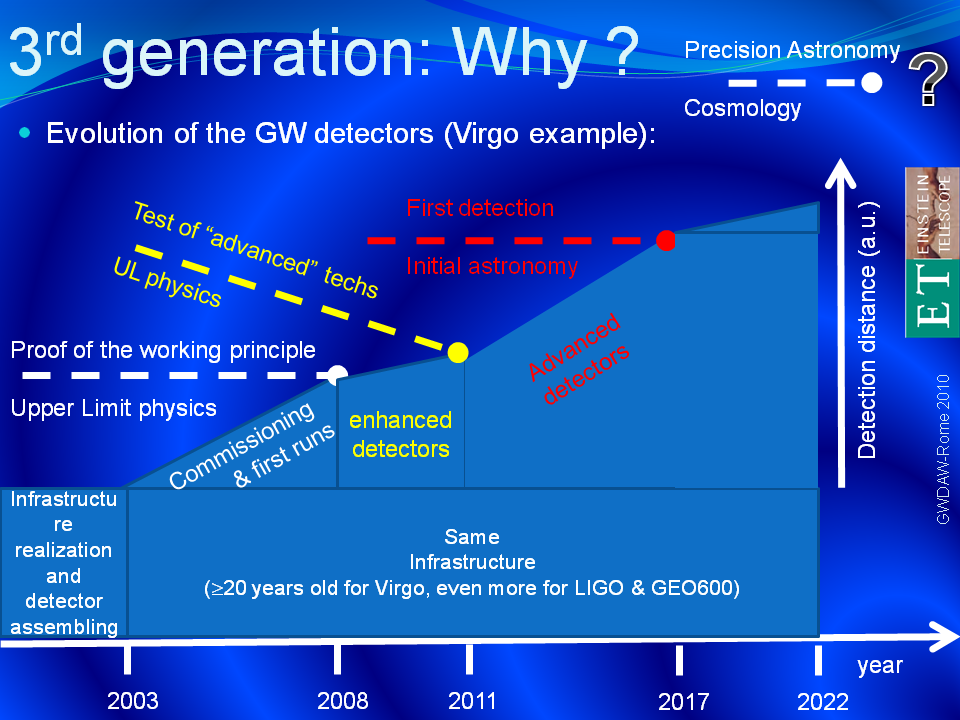
\includegraphics[width=0.99\textwidth]{Sec_Introduction/GWDAW-2010PunturoInfrastructureAdv.png}
%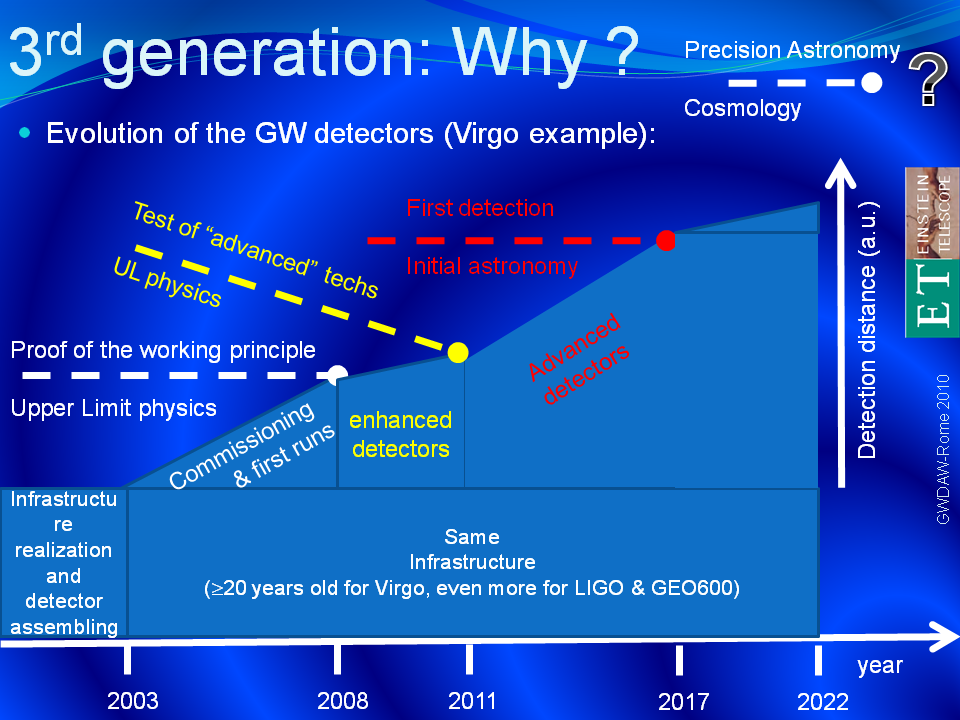
\includegraphics[width=0.9\textwidth, bb=0 0 800 600]{Sec_Introduction/GWDAW-2010PunturoInfrastructureAdv.png}
%\includegraphics[width=0.49\textwidth, bb=0 0 800 600]{ET-B.png}
\caption{Evolution of the first and second generation GW detectors. Time is 
on the horizontal axis, detector performance in the vertical one. When the 
advanced detectors will be operative the hosting infrastructures will be more 
than 20 years old and any further improvement of performance (sensitivity) 
will be suppressed by the limitation imposed by the infrastructures. (slide 
presented by M.\,Punturo at the GWDAW meeting, Rome Jan.\,2010).}
\label{Fig:InfraEvolution}
\end{figure*}
%%%%%%%% box ET in 1 minute
\clearpage
\etbox{h}{ETin1minute}{The Einstein Telescope at a glance}{
The \emph{Einstein gravitational--wave Telescope} will be an observatory of 
the third generation aiming to reach a sensitivity for GW signals emitted by 
astrophysical and cosmological sources about a factor of 10 better than the 
advanced detectors currently being built. An observatory with such a level of 
sensitivity will open the era of routine GW astronomy. \\[5pt]
An artist's impression of ET is given in Fig.\,~\ref{fig:ET_artists_view}, below. 
The main purpose of the ET project is the realisation of an infrastructure (an 
``observatory") capable of hosting more than one GW detector. This 
infrastructure will be usable for many decades, while the implemented detectors 
will undergo successive upgrades or replacements according to the current 
state of the art of interferometer technologies.
\begin{figure}[H]
	\centering	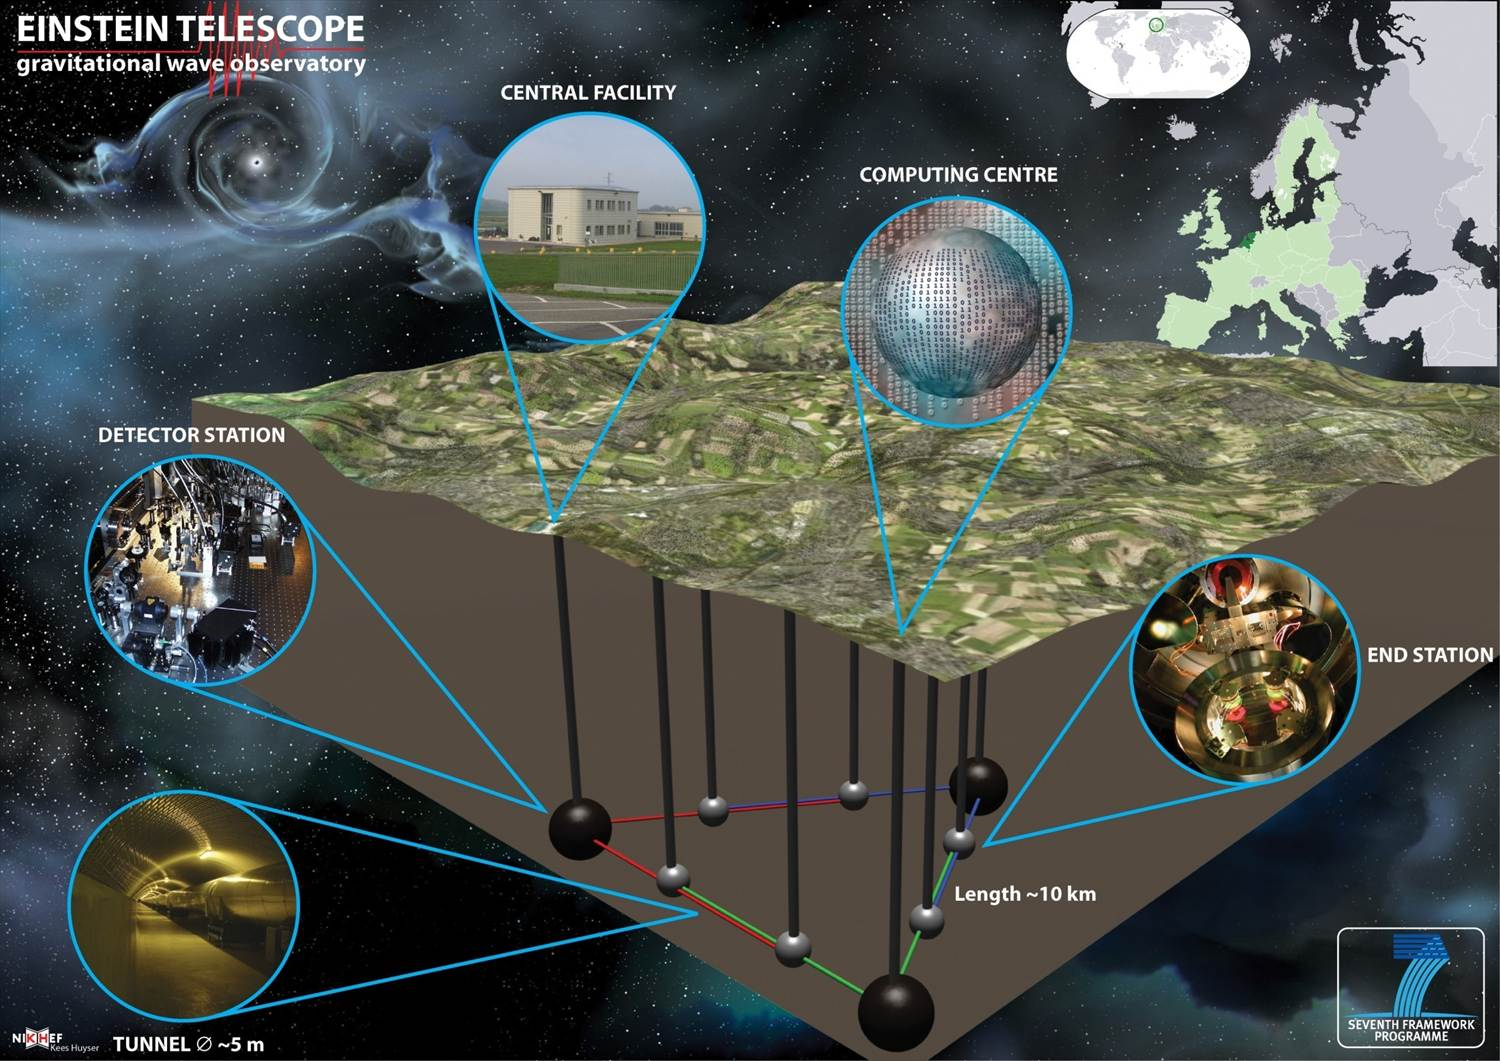
\includegraphics[width=0.80\textwidth]{Sec_Introduction/ET_artists_view.jpg}
	\caption{Artist's view of the Einstein Telescope}
	\label{fig:ET_artists_view}
\end{figure}
To reduce the effect of the residual seismic motion, thus allowing a better 
sensitivity at low frequencies (between 3 and 100\,Hz), ET will be located 
underground at a depth of about 100\,m to 200\,m and, in the complete 
configuration, it will consist of three nested detectors, each in turn composed 
of two interferometers (\emph{xylophone} configuration). The topology of 
each interferometer will be the dual-recycled Michelson layout with Fabry--Perot 
arm cavities, with a length of about 10\,km. The xylophone configuration of 
each detector devotes one interferometer to the detection of the low-frequency 
components of the GW signal (2--40\,Hz) while the other is dedicated to the 
high-frequency components, each interferometer adopting different, optimal 
technologies. In the former (ET-LF), operating at cryogenic temperature, the 
thermal, seismic, gravity gradient and radiation pressure noise sources will 
be particularly suppressed; in the latter (ET-HF) the sensitivity at high 
frequencies will be improved through the  high laser light power circulating 
in the Fabry--Perot cavities, and through the use of frequency-dependent 
squeezed light technologies. The target sensitivity of the ET observatory, at 
the current level of understanding, is shown in figure~\ref{fig:ET_sensitivity}.
}
%%%%%%%% end box ET in 1 minute

%%%%%begin info box on gravitational wave
\etbox{i}{box:detecting_gw}{Detecting Gravitational Waves}{
Gravitational waves change distances between objects, while the objects 
themselves locally remain at rest, by changing the metric of space-time. These
changes occur with opposing sign for orthogonal directions, as illustrated in 
figure~\ref{fig:GWeffect} for one polarisation of a gravitational wave incident 
perpendicular to the paper ($h_+$: see box~\ref{box:response} for more details).
\begin{figure}[H]
		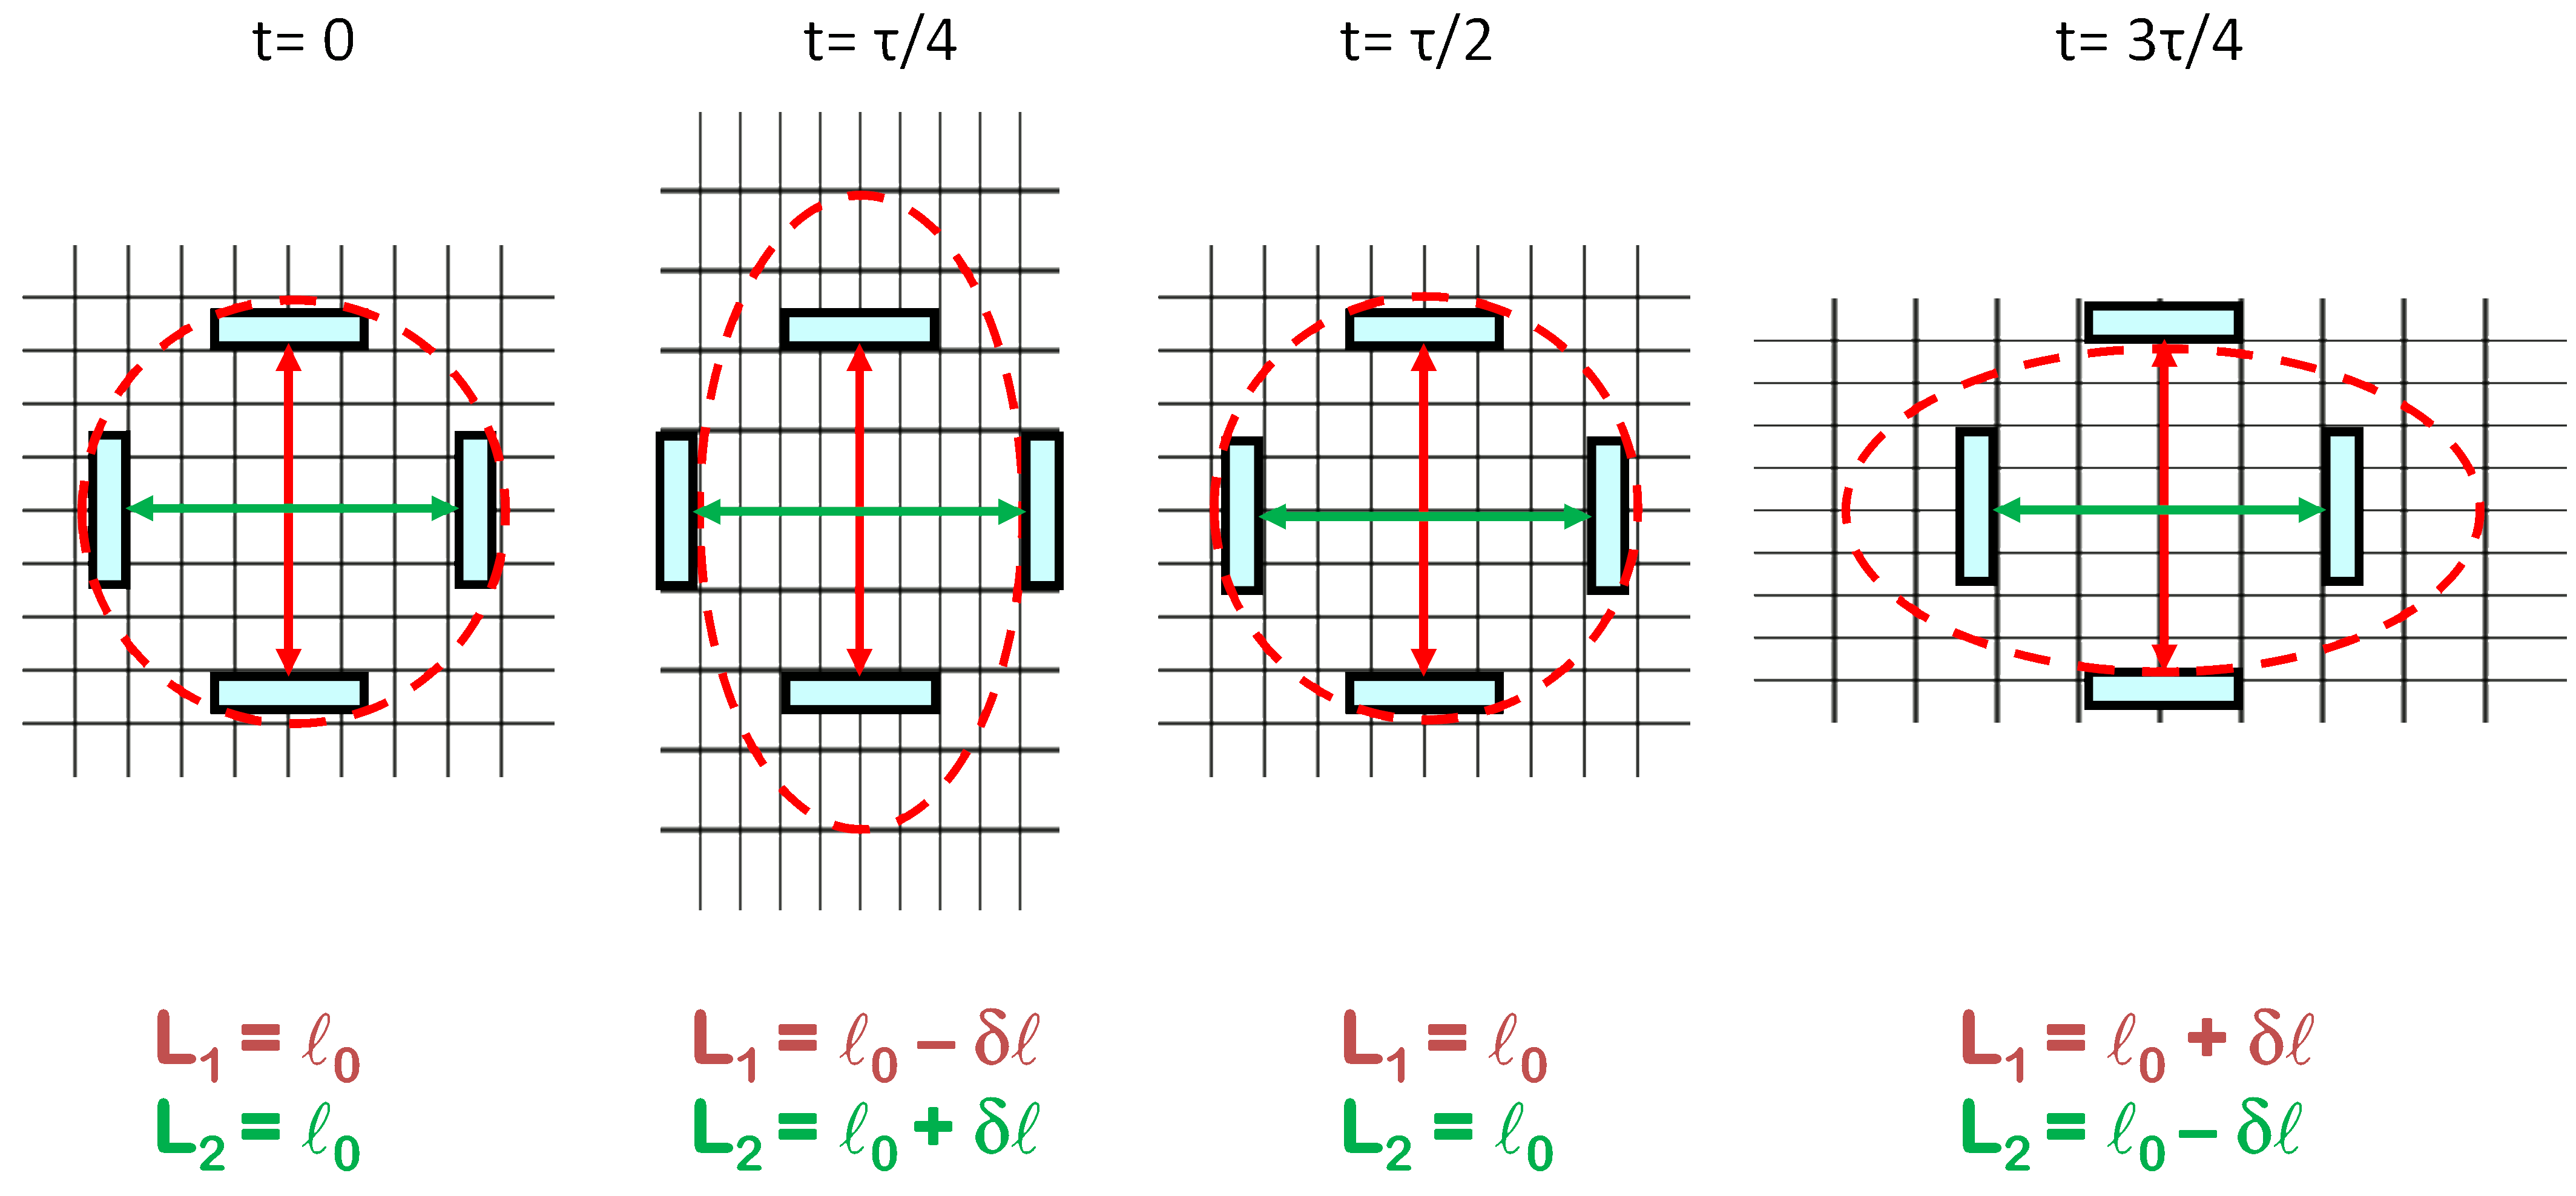
\includegraphics[width=\textwidth]{Sec_Introduction/GWeffect.png}
\vskip 0.3cm
	\caption{The effect of gravitational waves on the distances between objects. 
	While the mirrors remain locally at rest the metric gets changed by the 
	gravitational wave. The figure shows the effect of a sinusoidal 
	gravitational wave with period $\rm{\tau}$, for different times t. The 
	distances measured between the mirrors change by $\pm\delta\ell$.}
\label{fig:GWeffect}
\vskip -0.5cm
\end{figure}
A Michelson interferometer is ideally suited to measuring this effect. The 
measurement principle is shown in figure~\ref{fig:GWdetection}. A laser beam 
is split into two partial beams, sent along the interferometer arms, where it 
experiences a phase shift by the metric change of the gravitational wave, is 
reflected at the end and returns to the beam splitter, where it is recombined. 
The interference condition at the beam splitter, i.e.\ the phase relation of the 
two returning beams, determines the intensity on the photo detector. Three 
different phase relations are shown in figure~\ref{fig:GWdetection}. The 
relative length change of the interferometer arms can hence be detected by 
measuring the power at the output port. Although the measurement principle 
is very simple, for getting the best possible sensitivity all influences that 
change the geometrical or optical arm length or that cause a signal in the 
detected photo-current mimicking a gravitational wave have to be minimised, 
resulting in very sophisticated and complex instruments.
\begin{figure}[H]
		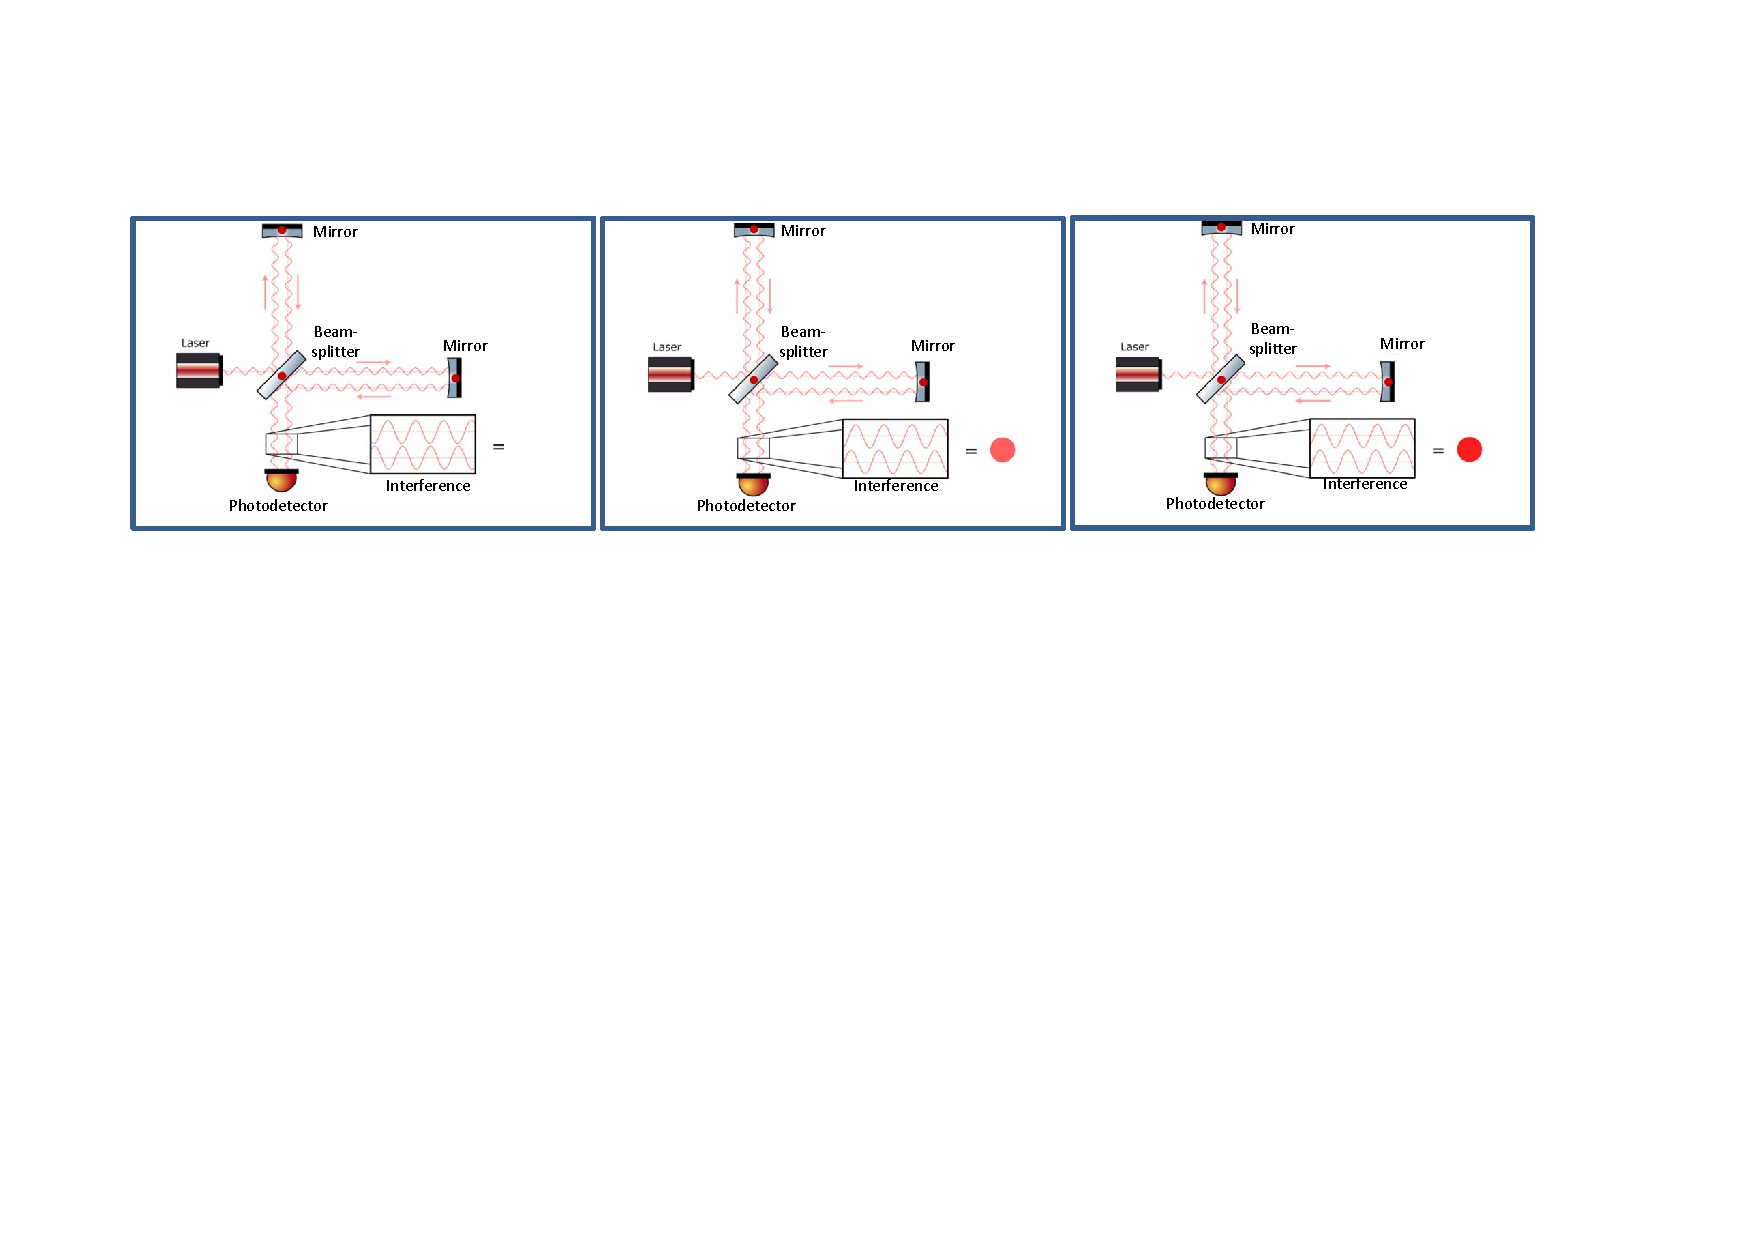
\includegraphics[width=\textwidth]{Sec_Introduction/GWdetection.pdf}
\vskip 0.3cm
	\caption{Michelson interferometer principle for gravitational wave 
	detection, showing three different interference conditions resulting in 
	different brightness at the output port.}
	\label{fig:GWdetection}
\vskip -0.6cm
\end{figure}
}

%%%%%end info box on gravitational wave

%
\subsection{Scientific targets of the ET observatory}
\subsubsection{Fundamental physics}
\label{ScienceCase:FundamentalPhysics}
Astronomical sources of gravitational waves are essentially
systems where gravity is extremely strong, and are often
characterized by relativistic bulk motion of massive objects.
The emitted radiation carries an uncorrupted signature of the
nature of the space-time geometry, and is thus an invaluable
tool to understand the behaviour of matter and geometry in
extreme conditions of density, temperature, magnetic fields
and relativistic motion. Here are some examples of how GW
observations can impact fundamental physics.

In Einstein's theory, gravitational radiation travels at the speed 
of light and has two polarization states. In alternative theories 
of gravity one or both of these properties might not hold, owing 
to the presence of massive gravitons, or a scalar field mediating 
gravity in addition to the tensor field. Current experimental
tests of gravity, as well those afforded by the data from the
Hulse-Taylor binary, are consistent with both Einstein's theory
and one of its alternatives called the Brans-Dicke theory.
Gravitational wave detectors will bring these theories
vis-a-vis observations that could decisively rule out one
or the other.

According to Einstein's gravity the space-time in the vicinity
of black holes is described by a unique geometry called the
Kerr solution. Observation of the radiation from the infall
of stellar-mass black holes into intermediate-mass black holes
will make it possible to test such uniqueness theorems. X-ray
astronomy has provided firm indirect evidence that intense
sources of X-rays may well host a black hole. An unambiguous
signature of the black hole geometry, however, could eventually
be provided by the detection of black hole quasi-normal modes:
gravitational radiation with characteristic frequencies and decay
times that depend only on the mass and spin angular momentum of the black hole.
Failure to detect such radiation from, for example, a newly
formed black hole would mean that gravity is more exotic than
we currently believe,
%(e.g., gravitational collapse might lead to entities called naked singularities)
and might reveal new phases of matter at extremely high densities.

The most attractive versions of string theory require a ten- or
eleven-dimensional space-time, far above those that we perceive.
In certain phenomenological models at the interface of string
theory and cosmology, what we perceive as a four-dimensional
Universe could be one part, or ``brane'', within a higher
dimensional ``bulk'' Universe. The extra spatial dimensions may
be compact and sub-millimetre-scale,
%(so-called ``Large Extra Dimensions'')
or even macroscopically large, if their geometry has
properties known as ``warping''. The key feature of brane-world
theories is that gravitational interactions, and in particular
gravitational waves, propagate in the bulk, while other interactions
are restricted to the brane, which partly explains why gravity is
so weak. 
%Brane world models predict a specific signature in the spectrum of gravitational waves. 
% [DON"T KNOW HOW WE CAN STAND BEHIND THIS SENTENCE, ITS 
% NOT SUPPORTED BY THE SCIENCE CASE]
Third-generation detectors offer 
the exciting possibility of observing radiation from the bulk and 
thereby exploring whether the Universe has large extra dimensions.
% SOME STUFF ABOUT HOW TO TEST STRING THEORY \& BRANES
% OR COMMENTS ON NEW PHYSICS IN GENERAL IN RELATION TO
% STOCHASTIC?



\FloatBarrier
\subsubsection{Relativistic Astrophysics}
Astronomy has revealed a Universe full of diverse and exotic
phenomena that remain enigmas decades after their discovery.
Supernovae are the end-states of stellar evolution, resulting in
gravitational collapse followed by a huge explosion of the formerly infalling matter.
Gamma-ray bursts are intense sources of gamma radiation that last
only a few seconds to minutes yet emit more energy than a star does
in its entire lifetime.
Radio pulsars are compact objects as massive as the Sun but only
about 10\,km in size, and the regularity of their radio pulses and
occasional glitches in that regularity have remained 
puzzles for a long time after their discovery three decades ago.
Transient radio sources thousands of light years away
are associated with magnetic fields so strong that the emitted radiation
could break down terrestrial radio stations.

The source in question in each case is believed to be couched in
dense environs and strong gravitational fields and, therefore,
a potential source of gravitational radiation. For example, gamma-ray
bursts could be produced by colliding neutron stars which are
electromagnetically invisible for most of their lives but are very
powerful emitters of GWs. Transient radio sources could be the
result of quakes in neutron stars with concomitant emission of GWs.
Observing such `multi-messengers' (sources that are strong emitters of
both EM and GW radiation) will help understand phenomena that
have remained puzzles for decades.

The centre of every galaxy is believed to host a compact
object a million to a billion times as massive as our Sun,
a powerful emitter of optical, radio and other radiation.
What is the nature of this object? How and when did it form?
Did it form from small 100-solar-mass seeds and then grow
by accreting gas and other compact objects? What is its
relation to the size of the galaxy as a whole? These are some
of the questions which a model of the formation of structure in
the Universe must answer.  While electromagnetic observations 
have provided valuable data, ET can explore the population of 
stellar mass and intermediate mass black holes as a function 
of redshift and shed light on black hole demographics, their 
mass distribution and growth.

ET will also be sensitive to
a population of sources at very high redshifts, helping us
study cosmological evolution of sources, the history of star
formation and its dependence on the matter content of
the Universe, and the development of large-scale structure in the
Universe.

\FloatBarrier
\subsubsection{Cosmology}
The twentieth century was the golden age of cosmology. With
the advent of radio and microwave astronomy it was possible to
finally address key questions about the origin of the
Universe.  The cosmic microwave background (CMB) is a relic radiation
from the hot Big Bang that is believed to have been the
initial condition for primordial nucleosynthesis. Since the early
Universe was very dense, this radiation was in thermal
equilibrium with matter for about 380,000 years after the Big
Bang and cannot directly reveal the conditions in the very
early phases of the Universe's history. The most direct way of
observing the primeval Universe is via the gravitational
window with a network of two or more detectors. From fairly
general assumptions one can predict the production of
a stochastic background of GWs in the early Universe, which travel
to us unscathed as a consequence of their weak coupling to matter.

The most amazing aspect of the Universe is that only about
4\% of its energy density appears in the form of visible matter,
the rest being dark matter and dark energy.
In order to understand the behaviour of these `dark' contents
it is necessary to have a standard candle---a population of
sources whose distance from Earth can be inferred from their
luminosity. 
Compact binaries are an astronomer's ideal standard candle. 
By measuring the signature of the gravitational radiation they emit,
it is possible to infer their intrinsic parameters (e.g.\ the
masses and spins of the component objects) and accurately
deduce their luminosity distance. In fact, compact binaries
eliminate the need to build a cosmic distance ladder---the
process by which standard candles at different distances are
calibrated in astronomy since there is no source that is
suitable at all distances.

The synergy of multi-messenger astronomy is nowhere more
apparent than in the use of standard sirens of gravity to
test the concordance model of cosmology.  ET might detect
several hundred compact binary coalescence events each year
in coincidence with short-hard gamma-ray bursts, provided, of
course, the two are related.  While gravitational observations would
provide an unambiguous measure of the luminosity distance,
the host galaxy of the GRB could be used to measure the
redshift. By fitting the observed population to a cosmological
model, it will be possible to measure the Hubble parameter,
dark matter and dark energy densities, as well as the
dark energy equation-of-state parameter.

The early history of the Universe may have witnessed
several phase transitions as the temperature decreased
through the energy scales of a Grand Unified Theory (GUT)
and electroweak symmetry-breaking, and eventually to the
current state in which we see four different fundamental
interactions. During some phase transitions, cosmic strings
form as one-dimensional topological defects at the
boundaries of different phases. Vibrations of these strings
at the speed of light can sometimes form a kink that emits a
burst of gravitational radiation. The spectrum of such radiation
has a unique signature that can help us detect cosmic strings
and measure their properties, and thus provide a glimpse of the
Universe as it underwent phase transitions.

Perhaps the most exciting discovery of the new window will
be none of the above. If astronomical history is any example,
gravitational astronomy should unveil phenomena and
sources never imagined in the wildest theories---a possibility
of any new observational tool.


\FloatBarrier
\newpage
\subsection{Layout of the detector}
%\emph{Authors: M.Punturo, H. Lueck} 

\begin{wrapfigure}{r}{0.6\textwidth}
\vskip -0.4cm
	\centering
		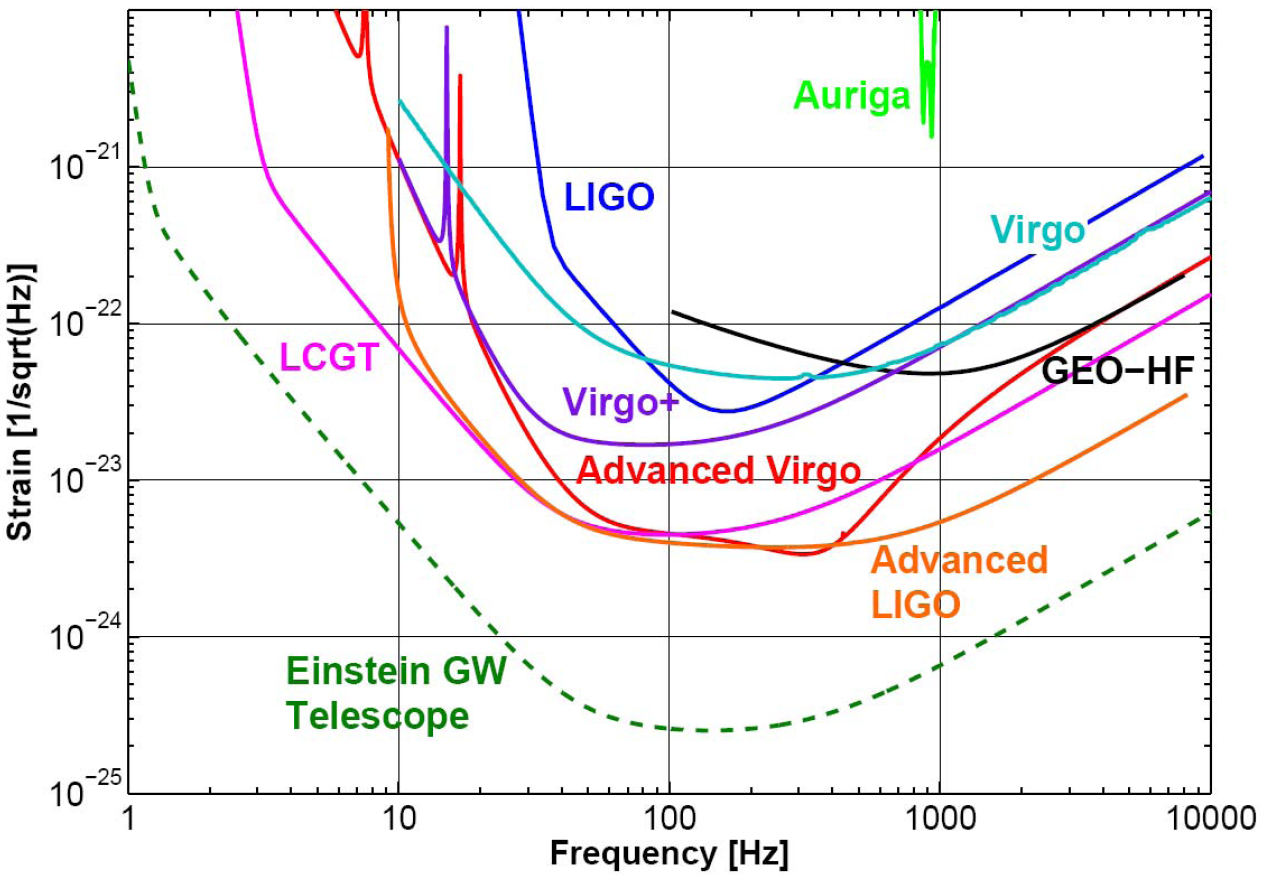
\includegraphics[width=0.6\textwidth]{Sec_Introduction/3gen_sens.png}
	\caption{Sensitivities of gravitational wave detectors from the first to the third generation.}
	\label{fig:GW_sens_evolution}
\end{wrapfigure}
The sensitivity of gravitational wave detectors improved considerably from 
the bar detectors to the first generation of interferometric detectors, which are 
currently being upgraded to the `advanced' generation. The corresponding 
sensitivities are shown in figure~\ref{fig:GW_sens_evolution}. 
In order to achieve the scientific goals stated above, the sensitivity in comparison 
to the second generation of gravitational wave detectors must be improved 
by about an order of magnitude over the entire detection frequency band ranging 
from 10\,Hz to about 10\,kHz. Frequent observation of low-frequency sources, 
e.g.\ intermediate mass black holes, requires an extension of the detection 
range towards lower frequencies. \\
The initial sensitivity goal for the Einstein Telescope, estimated at the start of 
the Design Study, as shown in figure~\ref{fig:GW_sens_evolution}, was driven 
by the need to get frequent high Signal to Noise Ratio (SNR) events for routine 
gravitational wave astronomy. The high-frequency sensitivity was given by the 
maximum power feasible, the mid-frequency range was governed by thermal 
noises and the low-frequency range by either thermal or seismic noises. The 
initial estimates have been refined during the design study and finally resulted 
in the sensitivity shown in figure~\ref{fig:ET_sens_evolution_2}.\\
\subsubsection{Size, shape and layout}
The conceptual design of a project of this financial scale (see 
table~\ref{Fig:TotalCostTable}) has to be based on well proven and 
experimentally tested techniques. To achieve the sensitivity that the Einstein 
Telescope project aims for, on the other hand, it will be necessary to exploit all 
state-of-the-art technologies and drive them to their physical limits.
\begin{wrapfigure}{r}{0.4\textwidth}
%\begin{figure}{H}
	\centering
		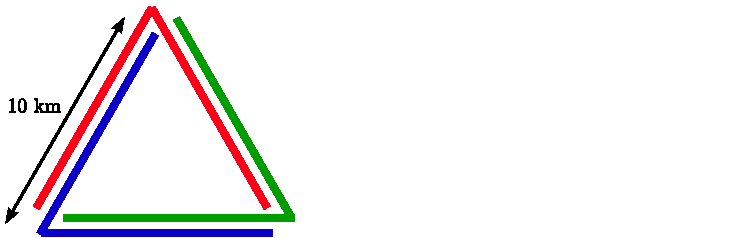
\includegraphics[width=0.3\textwidth]{Sec_Introduction/NestedDetectors.pdf}
	\caption{Three nested detectors in a triangular arrangement will 
	form the final Einstein Telescope geometry.}
	\label{fig:NestedDetectors}
\end{wrapfigure}
This sensitivity can only be reached by significantly increasing the size of the 
detector beyond the size of currently available instruments (i.e.\ 3\,km for Virgo 
and 4\,km for LIGO) and going to an underground location, where the seismic 
noise is lower than at the surface. Only by increasing the arm length to 10\,km 
can the influence of unavoidable displacement noises be lowered to a tolerable 
level.\\
In its final construction stage the Einstein Telescope will consist of three nested
detectors, which will be arranged in a triangular pattern as shown in 
figure\,~\ref{fig:NestedDetectors}. 
In contrast to the traditional L-shaped geometry of the first and second generations 
of gravitational wave detectors this arrangement is equally sensitive for both 
polarisations of the gravitational wave. Additionally it shows a more isotropic 
antenna pattern compared to the L-shaped detectors, as shown in 
figure\,~\ref{fig:response}. The overall frequency range covered will reach from 
a few Hertz to about 10\,kHz.

Each individual detector in turn will comprise two interferometers, one 
specialised for detecting low-frequency gravitational waves and the other one 
for the high-frequency part. The sensitivity goal for each interferometer is shown 
in figure\,\ref{fig:ET_sensitivity}. %\\
Each individual interferometer has a classical dual-recycled Michelson topology 
with arm cavities. This is a mature technique, well tested in laboratory 
experiments, and currently being set up for the second-generation detectors, 
Advanced LIGO and Advanced Virgo. More elaborate topologies like Sagnac 
interferometers or optical bars using Quantum Non-Demolition (QND) techniques 
do not promise significant advantages and have not yet reached the level of 
maturity required for a project of this scale.\\

\subsubsection{Quantum Noise} 
In order to achieve a sufficient sensitivity at high frequencies the light power in 
the arms of the high-frequency interferometer needs to be increased to the 
megawatt range. Thermal noise considerations on the other hand require cryogenic 
optics to reach the sensitivity goal at low frequencies. 

\begin{wrapfigure}{r}{0.6\textwidth}
%\begin{figure}{H}
	\centering
		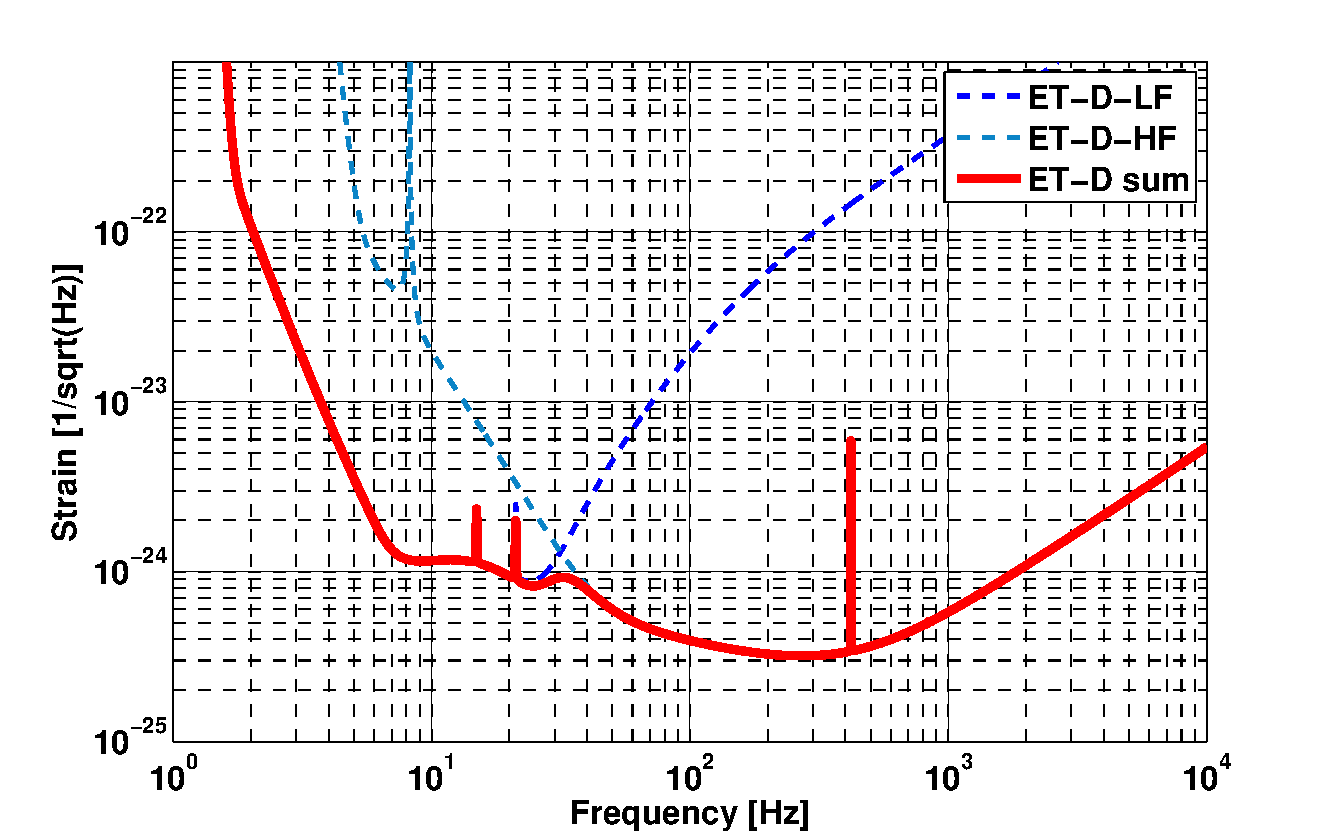
\includegraphics[width=0.6\textwidth]{Sec_Introduction/ET_D_spectrum.pdf}
	\caption{Sensitivity of the Einstein Telescope in the `xylophone' configuration. 
	The sensitivity of the low-frequency cryogenic interferometer is shown in the 
	dashed dark blue curve and the one of the high-frequency room temperature 
	one in a dashed blue-green tone. The sum of both is given by the solid bright red curve.}
	\label{fig:ET_sensitivity}
\end{wrapfigure}

Operating cryogenic optics at a level of several megawatt of light power presents 
a serious technological challenge which is extremely hard to master. Even for 
the best mirrors that state-of-the-art coating technology can produce, the 
residual absorption of only about one ppm leads to an absorbed power of 
several Watt at a circulating light power level in the megawatt range. The resulting 
thickness of the suspension fibres, which would be needed to remove the heat, 
would spoil the performance of the ultra low loss suspension. The Einstein 
Telescope will therefore be realised in what we call a `xylophone' arrangement, 
where each single detector is split into two interferometers, leading to sensitivities 
as shown in figure~\ref{fig:ET_sensitivity}. The one dedicated for detecting 
high-frequency gravitational waves in the range from about 30\,Hz to 10\,kHz 
will be operated at room temperature, use fused silica optics with a diameter of 
about 60\,cm and a mass of about 200 kg each, have a light power of about 3\,MW 
in the interferometer arms, and run with broadband tuned signal recycling. The 
cryogenic, low-frequency one, operated at a temperature of 10\,K and aimed at the 
frequency range from 1.5\,Hz to 30\,Hz, will use detuned signal recycling, have a 
light power of 18\,kW 
in the interferometer arms, and silicon mirrors with a diameter of about 40\,cm and 
a mass of about 200\,kg. The cryogenic optics will either be made of sapphire or, 
more likely, of silicon. The dimensions will partly be determined by the maximum 
available bulk material size and otherwise be comparable to the room temperature 
ones. A summary of the main parameters for the high and low temperature 
interferometers is given in table~\ref{tab:summary14}.\\
The high mirror mass will not only keep radiation pressure effects low but also 
allow larger sized beam spots on the mirror surfaces for lowering thermal noise 
effects. This split detector arrangement also offers an elegant solution for the 
challenge that radiation pressure noise and shot noise scale in opposite ways with 
light power and cannot individually be optimised in a single interferometer. In an 
interferometer using classical states of light the so-called Standard Quantum 
Limit (SQL) determines the lower limit for the quantum noise. For each frequency 
there is a different optimal compromise between shot noise and radiation pressure 
noise, meaning that in a single interferometer the SQL cannot be reached for all 
frequencies simultaneously. 
 
\begin{wrapfigure}{r}{0.35\textwidth}
%\begin{figure}{H}
	\centering
		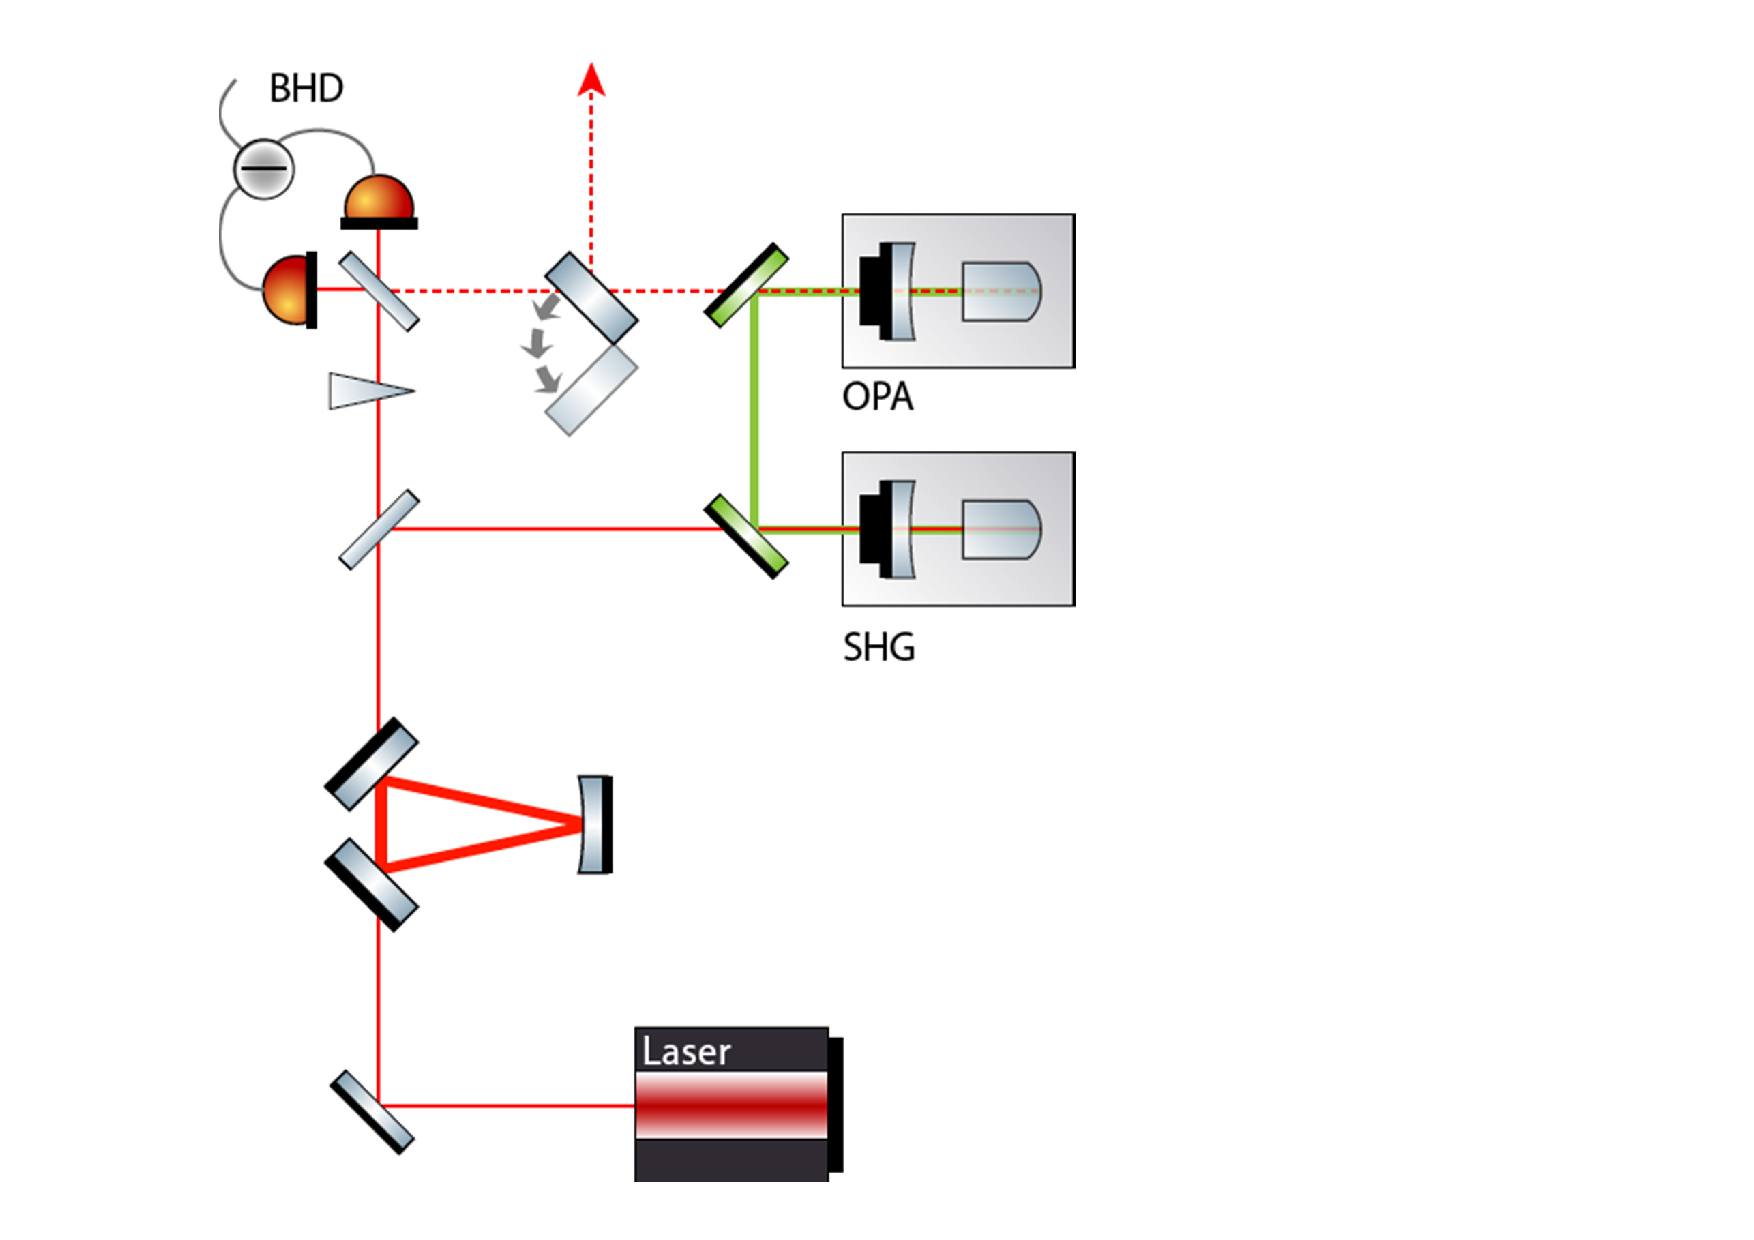
\includegraphics[width=0.35\textwidth]{Sec_Introduction/SqzGenIntro.pdf}
	\caption{Scheme for generating squeezed light. For details see section~\ref{subsec:SQZforGWD}}
	\label{fig:SqzGenIntro}
\end{wrapfigure} 

It can only be overcome if non-classical light with correlations between the phase 
and the amplitude quadratures is used, so-called squeezed light. In the shot noise 
dominated frequency range squeezed light is used, which shows lower phase 
fluctuations at the cost of the amplitude fluctuations in comparison to classical 
laser light in the interferometer arms. In the low-frequency, radiation pressure 
dominated range the fluctuations need to be lowered in the amplitude quadrature. 
This goal can be achieved by reflecting squeezed light off a filter cavity (see 
figure~\ref{Fig:opt_lay_over}). 

The usage of squeezed light is currently tested in the existing gravitational wave 
detectors and is foreseen as an add-on to the second generation. Squeezing 
levels over the full observation band width of up to 10\,dB, and stable long-term 
operation and best squeezing values of almost 13\,dB have been demonstrated~\cite{Eberle2010}. 
For the Einstein Telescope we assume 15\,dB initial squeezing 
level at the squeezing source and an effective squeezing level of 10\,dB to be 
available (equivalent in shot noise reduction to a laser power increase of a factor
of 10). 

The squeezing level, and with it the sensitivity improvement that can be reached, 
depends on the optical losses in the squeezer, the filtering optics, the interferometer, 
and all optical devices on the way to the photodetector, including the photodetector 
efficiency itself. Optical losses easily add vacuum fluctuations to the squeezed quadrature 
and hence reconvert squeezed light into classical light. It will therefore be essential 
to keep the optical losses as low as possible. Optical losses of 75\,ppm per round 
trip are currently achievable with state-of-the-art techniques and are used as a 
conservative estimate for the filter cavities.

\subsubsection{Thermal Noise}
\begin{wrapfigure}{r}{0.65\textwidth}
\vskip -0.6cm
%\begin{figure}{H}
	\centering
		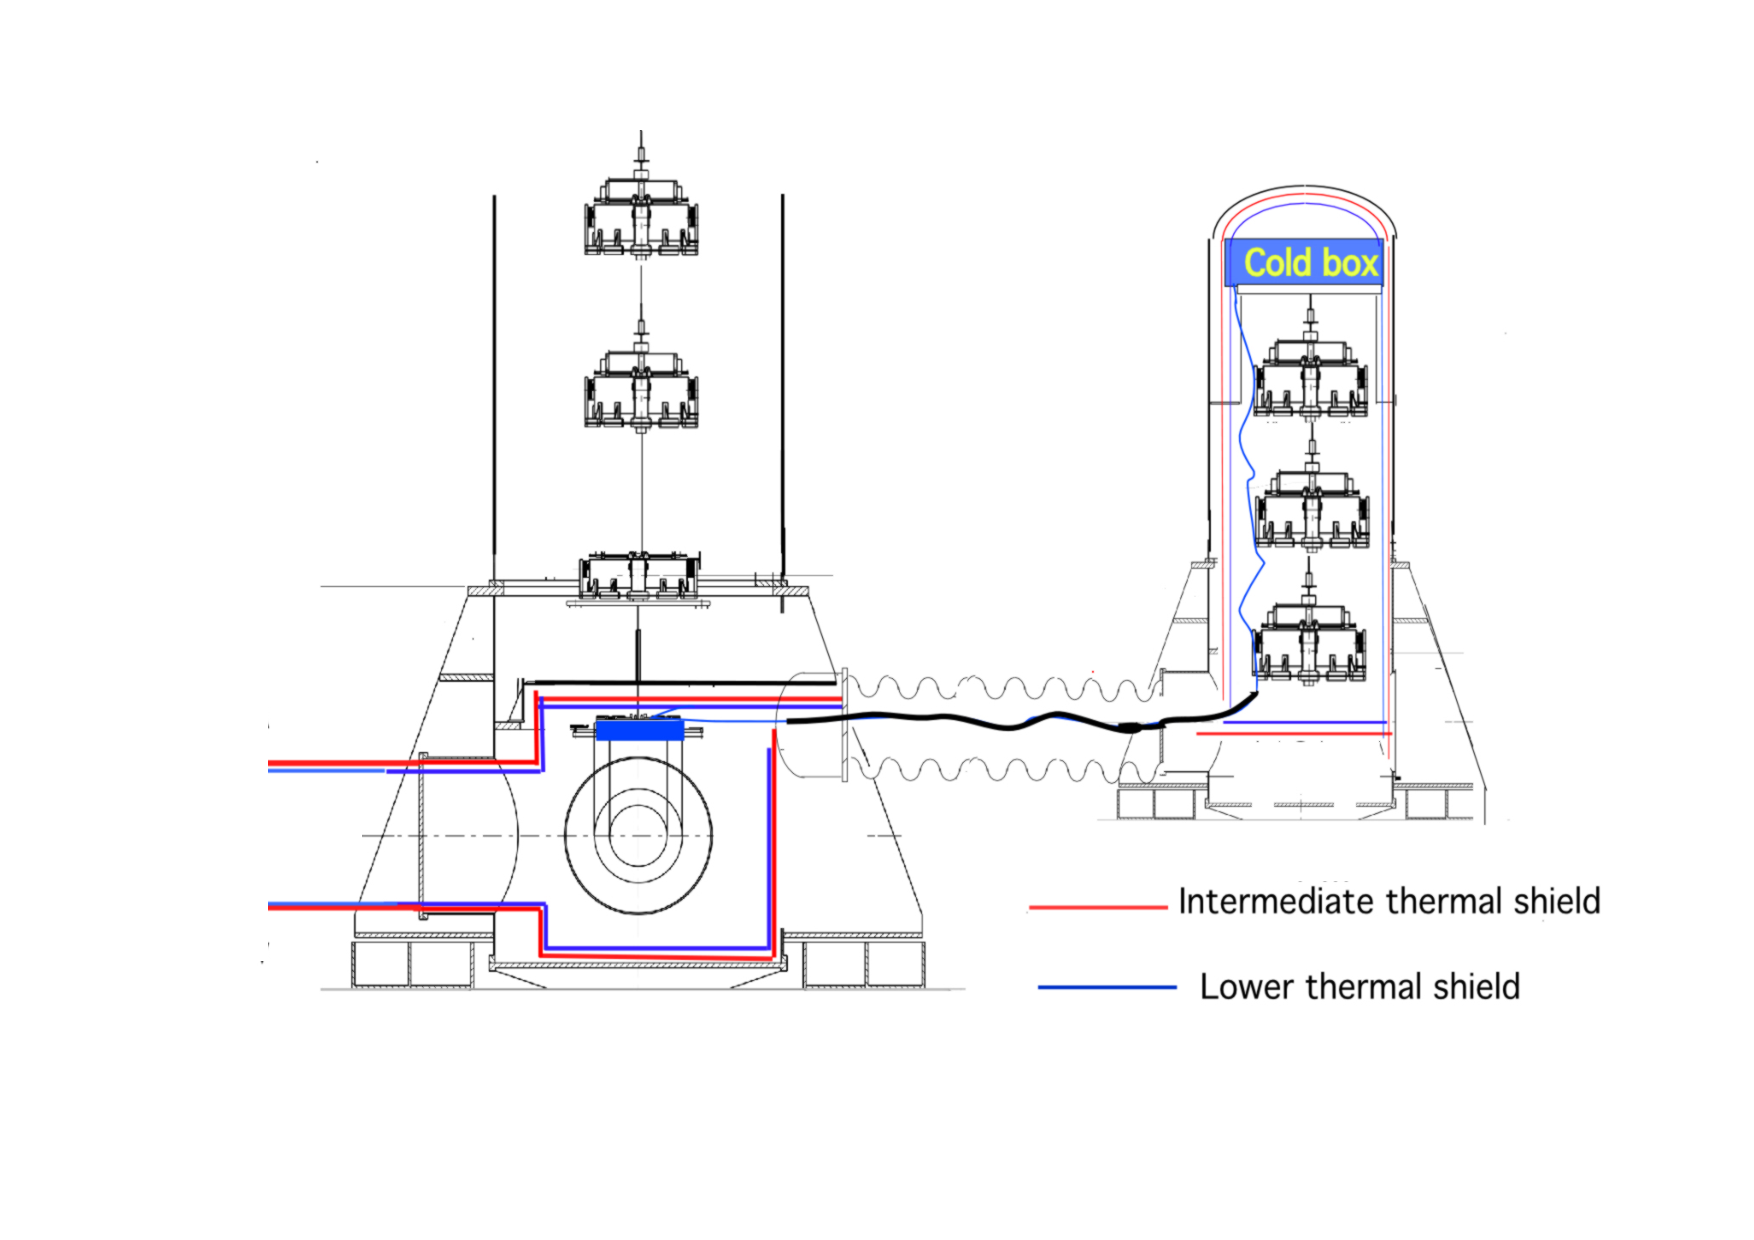
\includegraphics[width=0.6\textwidth]{./Sec_SiteInfra/Figures/ET_main-cryostat.pdf}
	\caption{Scheme for cooling the mirrors. For details see section~\ref{cryo}}
\vskip -0.1cm
\end{wrapfigure} 

Reaching the sensitivity goal at low frequencies requires a significant reduction 
of thermal noises compared to the first and second generations of gravitational-wave 
detectors, which can be achieved by operating the mirrors at cryogenic temperatures 
as low as 10\,K.  

Cryogenic operation is also foreseen for the final stage of the planned Japanese 
gravitational wave detector LCGT. At these low temperatures fused silica has a low 
mechanical quality factor and becomes unusable. Silicon and sapphire show 
excellent low-temperature behaviour (see section~\ref{sec:app}) and are good 
candidates for cryogenic gravitational wave detectors. Its availability in large 
quantities and good purity through the semiconductor industry makes silicon a 
promising candidate for the Einstein Telescope cryogenic optics. Some quantities 
such as the temperature dependence of the refractive index at low temperatures 
and the residual optical absorption in ultra pure silicon, although assumed to be 
good enough for use in ET, are currently not known and need to be 
investigated in R\&D activities.

Removing the heat generated by laser light being absorbed at the mirror surfaces 
without introducing excess vibration levels poses another technical challenge. As 
thermal radiation does not provide sufficient coupling at cryogenic temperatures 
this heat removal has to be done by thermal conduction of the suspension fibres. 
The resulting requirement for the thickness of the silicon suspension fibres needs 
to be balanced against good seismic isolation properties of thin fibres. The vibration 
level of cryo coolers, which could be placed close to the optics, threatens the 
low-frequency sensitivity (see section~\ref{sec:cryocoolers}). R\&D in active and 
passive vibration suppression is still required to sufficiently cut the remaining noise 
level down for use in the Einstein Telescope. Cryo fluids, like superfluid Helium\,II, 
which are cooled down at a remote location above ground, are available as a 
seismically more quiet alternative (see section~\ref{sec:Helium_II}). The final operating 
temperature for ET remains to be fixed in a technical design 
phase. The cooling capabilities foreseen so far will allow mirror temperatures 
as low as 10\,K.

\subsubsection{Seismic Isolation}

\begin{wrapfigure}{r}{0.4\textwidth}
\vskip -0.4cm
%\begin{figure}{H}
	\centering
		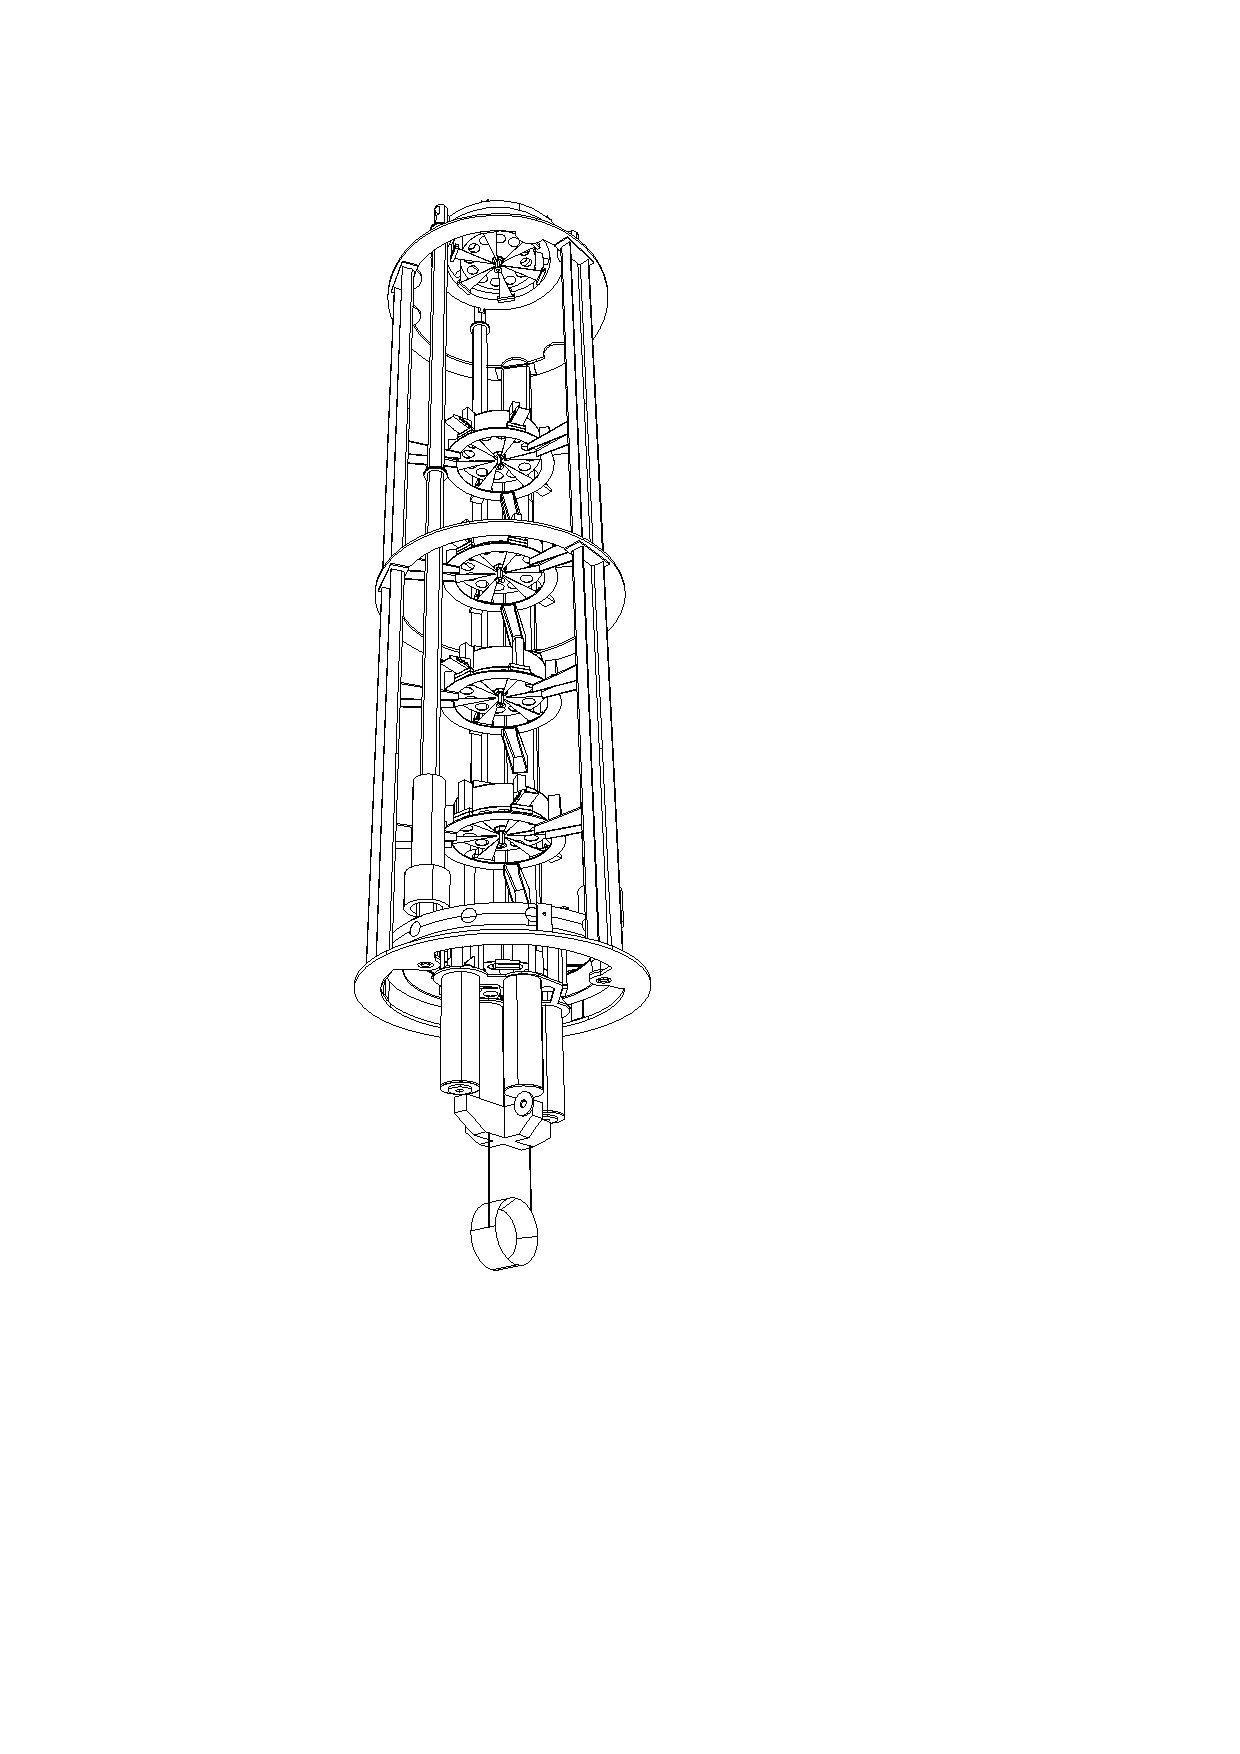
\includegraphics[width=0.18\textwidth]{./Sec_Introduction/VirgoSA.pdf}
\vskip 0.3cm
	\caption{Schematic view of the Virgo Superattenuator. See also section~\ref{sec:suspension_systems}}
\vskip -0.6cm
\end{wrapfigure} 

The main optics for the Einstein telescope need to be very well isolated against 
seismic ground motion. For the second generation of gravitational wave detectors 
both active and passive isolation strategies are being pursued. In the advanced 
LIGO detectors a two stage system actively isolates a platform from ground 
motion, from which the main optics are suspended by quadruple pendulums. The 
passive strategy employed at the Virgo detector demonstrated an excellent 
performance over the full frequency range (see figure \ref{FigSusp5}) and is foreseen 
as the reference solution for the Einstein telescope. The horizontal isolation is 
achieved with a six-stage pendulum system, whereas for the vertical degree of 
freedom cantilever springs  are used. The pendulum suspension system itself is 
supported by a platform resting on an inverted pendulum, which provides 
additional horizontal seismic isolation (see figure~\ref{SAfig1}). All mechanical 
resonances of the whole structure are actively damped to avoid resonant 
mechanical amplification of ground motion. The overall height of the suspension 
system is about 17\,m, requiring correspondingly tall vacuum chambers and caverns.

\subsubsection{Newtonian gravity gradient noise}
Newtonian gravitational interactions between the optics and the surrounding soil 
provide a direct coupling mechanism of ground motion to the interferometer test 
masses (see also section~\ref{NewtonianNoise}). As the resulting, so-called 
gravity gradient noise cannot be shielded from the mirrors, a location has to be 
found where this seismic motion is minimal and the surrounding soil as 
homogeneous as possible. This goal can be achieved in an underground location 
in a seismically quiet region. Preliminary measurements show that a depth of 100 to 
200\,m in a remote location with low population density provides sufficiently low 
seismic motion. The potential of measuring the ambient seismic motion, feeding 
it into a gravity gradient noise model, and then subtracting the predicted effect 
from the interferometer output signal has been investigated. Initial results are 
promising, and are interesting also for the second generation of gravitational 
wave detectors, but investigations need to be continued in an R\&D programme 
(see section~\ref{subsub:AmbientNNsubtraction}).

\subsubsection{Vacuum}
The space between the mirrors in the interferometer arms has to be evacuated 
to very low residual partial gas pressures to keep the apparent length changes 
caused by fluctuations of the refractive index sufficiently low. The tolerable 
maximum pressure is on the order of $10^{-8}$\,Pa (see paragraph~\ref{average pressure}).
 
Some technical parameters will remain ``to be defined'' in this design study 
document. At this stage of the conceptual design these parameters are not 
important and will be worked out in a future technical design phase.

\subsubsection{\label{Noisebudget}Noise budget}

\begin{wrapfigure}{r}{0.60\textwidth}
  \begin{center}
\vskip -0.3cm
    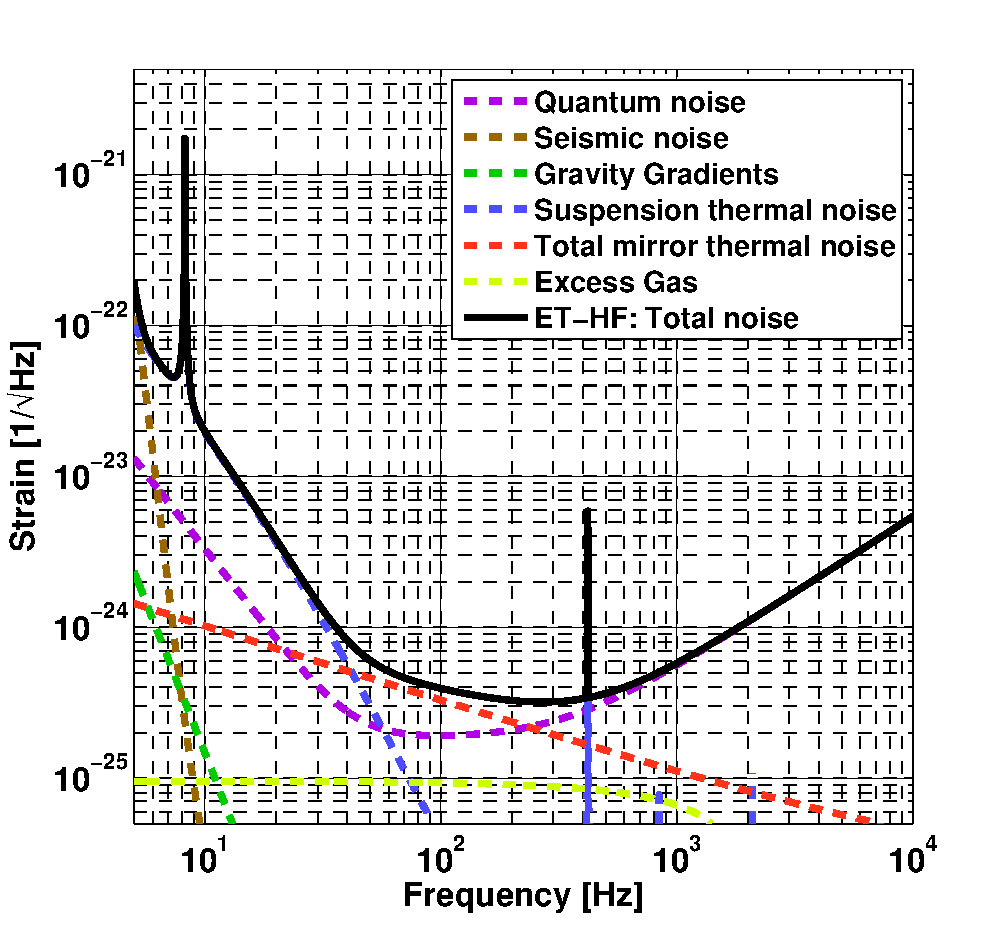
\includegraphics[width=0.45\textwidth]{Sec_Introduction/ETD_HF3.pdf}
%      \end{center}
%  \end{wrapfigure}
%  
% \begin{wrapfigure}{r}{0.6\textwidth}
%  \begin{center}
\vskip 0.4cm
    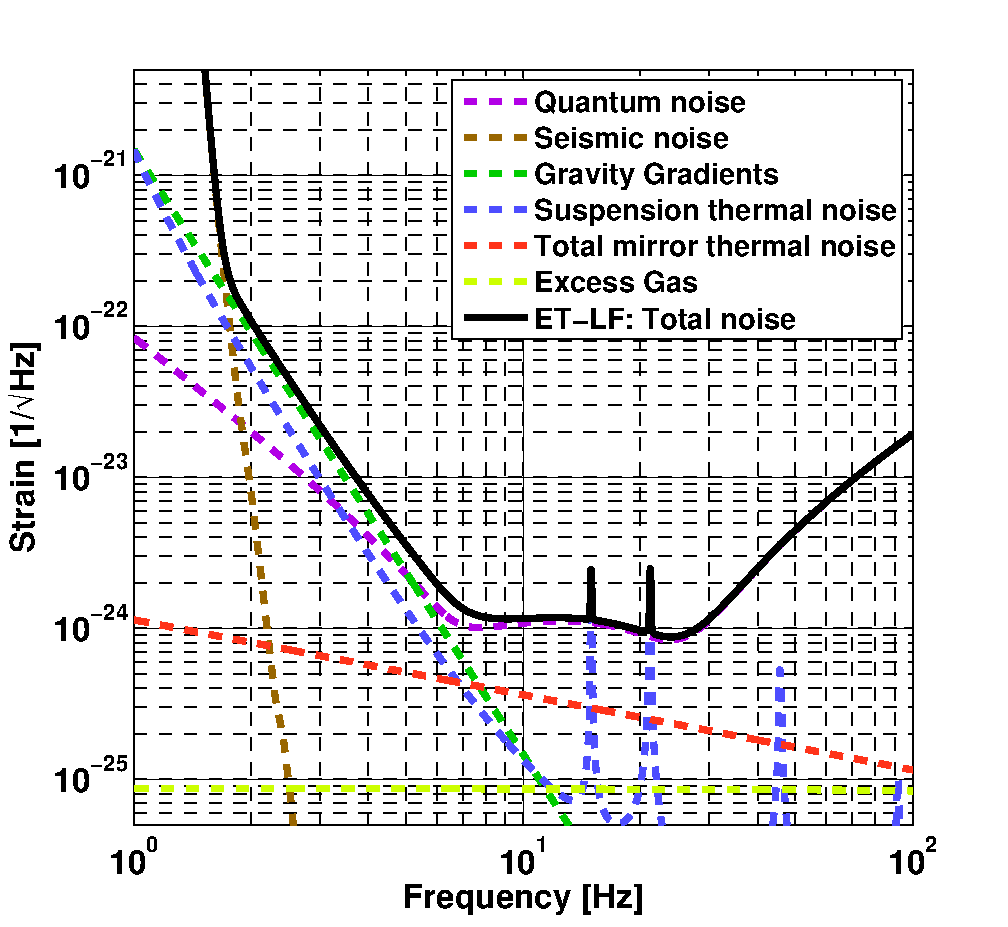
\includegraphics[width=0.45\textwidth]{Sec_Introduction/ETD_LF3.pdf}
    \caption{Noise budget for the low- and high-frequency interferometer for the 
    parameters used for the ET-D sensitivity curve as stated in table~\ref{tab:summary14}.}
    \label{fig:noise_budget}
    \vspace{-0.7cm}
  \end{center}
\end{wrapfigure}

The xylophone strategy, i.e.\ the division of each detector into a low-frequency 
and a high-frequency interferometer, allows to pursue different strategies in 
optimising the noise for each frequency range. The noise budget for the 
high-frequency interferometer is shown in the upper part of figure~\ref{fig:noise_budget}. 

In the frequency range from about 7\,Hz to 30\,Hz the sensitivity is limited by
suspension thermal noise, resulting from the interferometer being operated 
at room temperature. At frequencies above 500\,Hz the dominating noise 
source is photon shot noise. Between these two frequency ranges mirror 
thermal noise is limiting the overall sensitivity. In the noise budget for the 
low-frequency interferometer, shown in the lower part of 
figure~\ref{fig:noise_budget}, quantum noise is limiting the sensitivity over 
the entire frequency range above 7\,Hz. Due to the operation at cryogenic 
temperatures the influence of suspension thermal noise in the frequency 
range above 7\,Hz can be cut down to a sufficiently low level. Below 7\,Hz 
the sensitivity is limited by comparable amounts of quantum noise, 
gravity gradient noise, and suspension thermal noise. Due to the good 
performance of the multistage pendulum suspensions the influence of 
seismic noise can be limited to the frequency range below 2\,Hz. Investigations 
of new quantum non-demolition techniques in a planned R\&D program will 
show whether it is possible to cut down the quantum noise contributions to 
an even lower level in the frequency range from 7\,Hz to 30\,Hz.

\FloatBarrier
\clearpage
\subsection{Layout of the observatory}
%\emph{Authors: M.Punturo, H. Lueck} \\

\begin{wrapfigure}{r}{0.6\textwidth}
\centering
\vskip -0.35cm
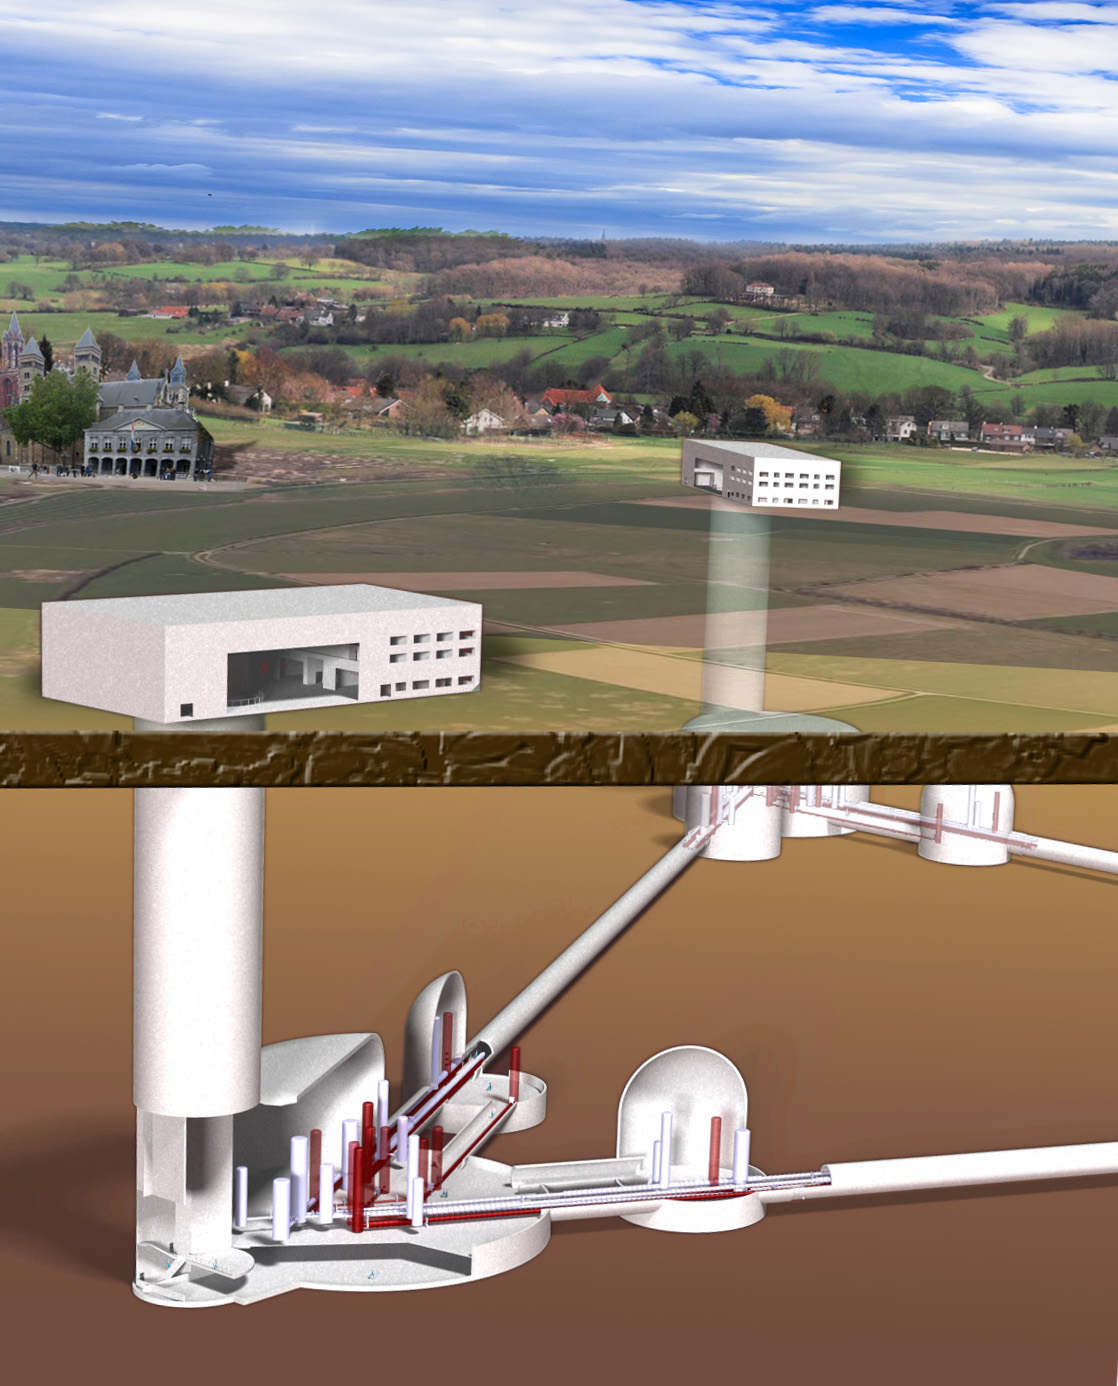
\includegraphics[width=0.6\textwidth]{Sec_Introduction/ArtisticViewBuildings.jpg}
\vskip 0.3cm
\caption{Artistic view of the arrangement of buildings, access shafts and underground caverns.}
\vskip -0.1cm
\label{Fig:Buildings}
\end{wrapfigure} 

As a consequence of the extremely demanding seismic requirements the Einstein 
Telescope will be located underground at a depth of about 100\,m to 200\,m and 
will, in the complete configuration, consist of three nested detectors, each in turn 
composed of two interferometers. Selecting the geometry of an equilateral triangle, 
where each side of the triangle is simultaneously used by two detector arms, allows 
to determine the polarisation of the gravitational wave and optimises the usage of 
the tunnels. The topology of each interferometer will be the dual-recycled Michelson 
layout with Fabry-Perot arm cavities. An artist's impression of the Einstein Telescope 
is shown in figure~\ref{fig:ET_artists_view}. \\
Underground seismic measurements at eight different European locations have 
been performed within this design study and additional measurements from 
external sources have also been evaluated. Satisfactory seismic performance has 
been found in several locations. 

For the final site selection long-term seismic noise measurements including 
seasonal effects like variable wind speeds and ocean wave height need to be made, 
and other nonscientific factors of influence (e.g.\ political, financial, interest of local 
parties, vicinity to research institutions) have to be included in the decision process.

The sensitivity curve shown in figure~\ref{fig:ET_sensitivity} gives the sensitivity for 
a single detector with 10\,km arm length and an angle of $90^{\circ}$ between the 
arms. This is done for better comparison with the existing detectors and their 
`advanced' versions. ET will in fact have three 10\,km detectors and the angles 
between the arms will be $60^{\circ}$. The resulting sensitivity in comparison with 
a single $90^{\circ}$ detector depends on the source location in the sky and its 
orientation, as the angular antenna pattern (see figure \ref{fig:triangleAP}) and the 
polarization dependence (independent in the triangular case) influence the signal 
strength differently for different detector layouts. On average the sensitivity of the 
triple $60^{\circ}$ detector is slightly better than a single, optimally oriented $90^{\circ}$ one.


\etbox{h}{ETSensitivityCurves}{Sensitivity curves for the Einstein Telescope}{
As the understanding of the achievable sensitivity of the Einstein Telescope evolved 
throughout the Design Study, different sensitivity curves are used in this document, 
named from ET-B to ET-D (see figure~\ref{fig:ET_sens_evolution_2}).\\ 
The very first, preliminary sensitivity curve ET-A was a crude, early estimate and 
will hence not be used in this document. 
ET-B is the sensitivity curve where each detector is built from a single interferometer, 
where the high power needed to achieve good high-frequency performance 
compromises the low-frequency performance. Over a wide frequency range from 
a few Hertz to a few times 10\,Hz the sensitivity is limited by radiation pressure noise, 
whereas above a few hundred Hertz the sensitivity is limited by shot noise.\\
The next evolutionary step is the sensitivity curve ET-C, where each detector is 
split into two interferometers, each dedicated to a distinct frequency range (the 
xylophone configuration). Some technical details, such as losses inside optical 
resonators are not fully included in this sensitivity curve.\\
The latest sensitivity curve is given by ET-D, where imperfections like optical 
losses in cavities are included in the computations. As the later sensitivity curves 
became available only during the Design Study, some of the subsection results 
are still based on earlier versions, which will be indicated by the sensitivity curve 
acronym.\\
In the cost optimisation phase towards the end of the design study some 
parameters have been changed with respect to the ET-D sensitivity parameters, 
e.g.\ the lengths of the filter cavities for the high frequency interferometers, but 
have only an insignificant (<10\%) influence on the overall sensitivity.
\begin{figure}[H]
	\begin{center}
		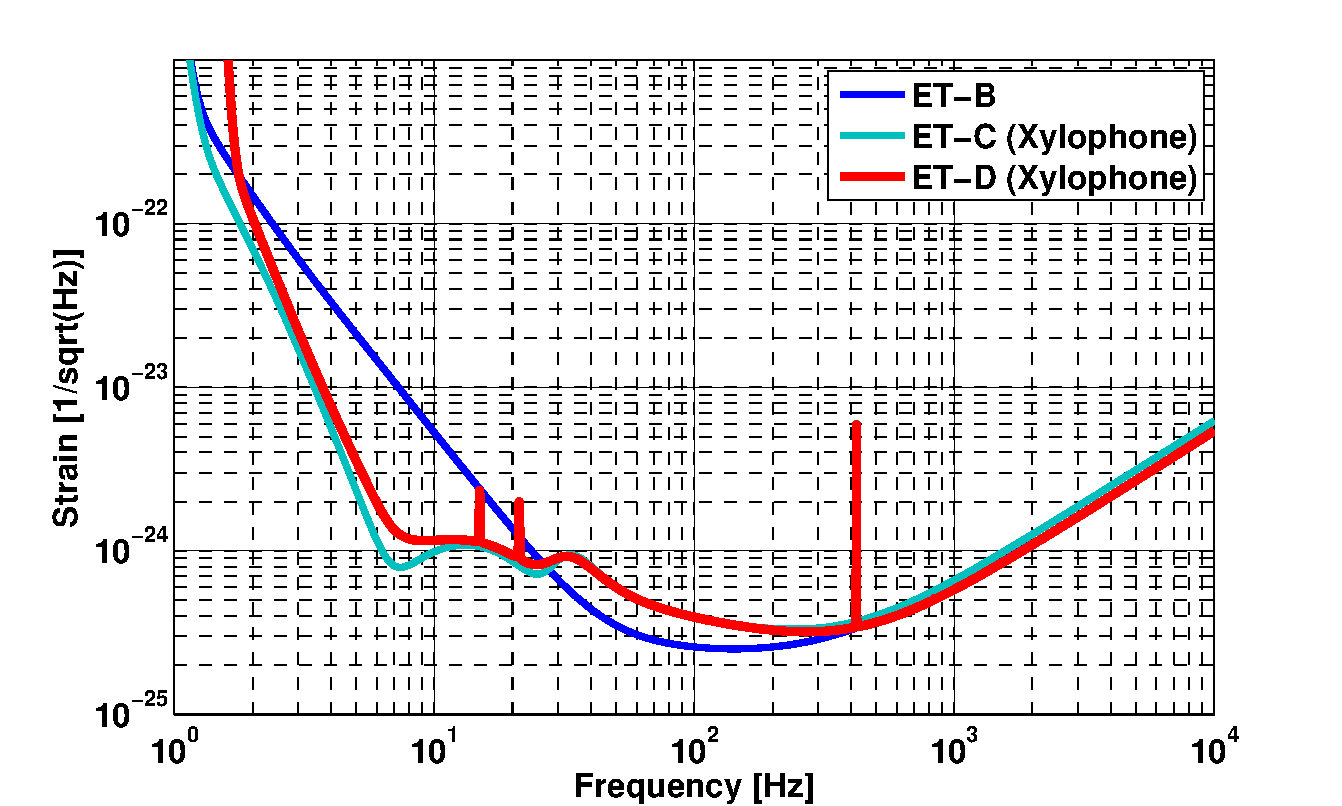
\includegraphics[width=0.7\textwidth]{Sec_Introduction/all_sens3.pdf}
\vskip 0.3cm
	\caption{Sensitivity curves for ET used in this document. For details see text.}
	\label{fig:ET_sens_evolution_2}
	\end{center}
\vskip -0.4cm
\end{figure}
}
For the desired sensitivity an overall side length of the triangle of about 10\,km is 
required. More specifically in this document we assume 10\,km for the arm cavity 
length as depicted in figure~\ref{fig:infra2} and figure \ref{Fig:Simple_ETv1} and an
additional 300\,m of tunnel length for telescopes for mode matching the large 
beam size from the interferometer arms to smaller beams in the beam splitter area. 
This gives a total triangle side length of 10.3\,km and an overall tunnel length for 
the Einstein Telescope Observatory of 30.9\,km. This length of 300\,m from the ``vertex 
station'' to the ``satellite station'' is also used for the filter cavities for the high-frequency 
interferometer housed in a separate tunnel, which simultaneously serves as a safety 
escape route from the ``satellite caverns'' (see figure\,\ref{shaftaccess} and figure,\ref{infra}.  

\begin{wrapfigure}{r}{0.66\textwidth}
	\centering
\vskip 0.1cm
		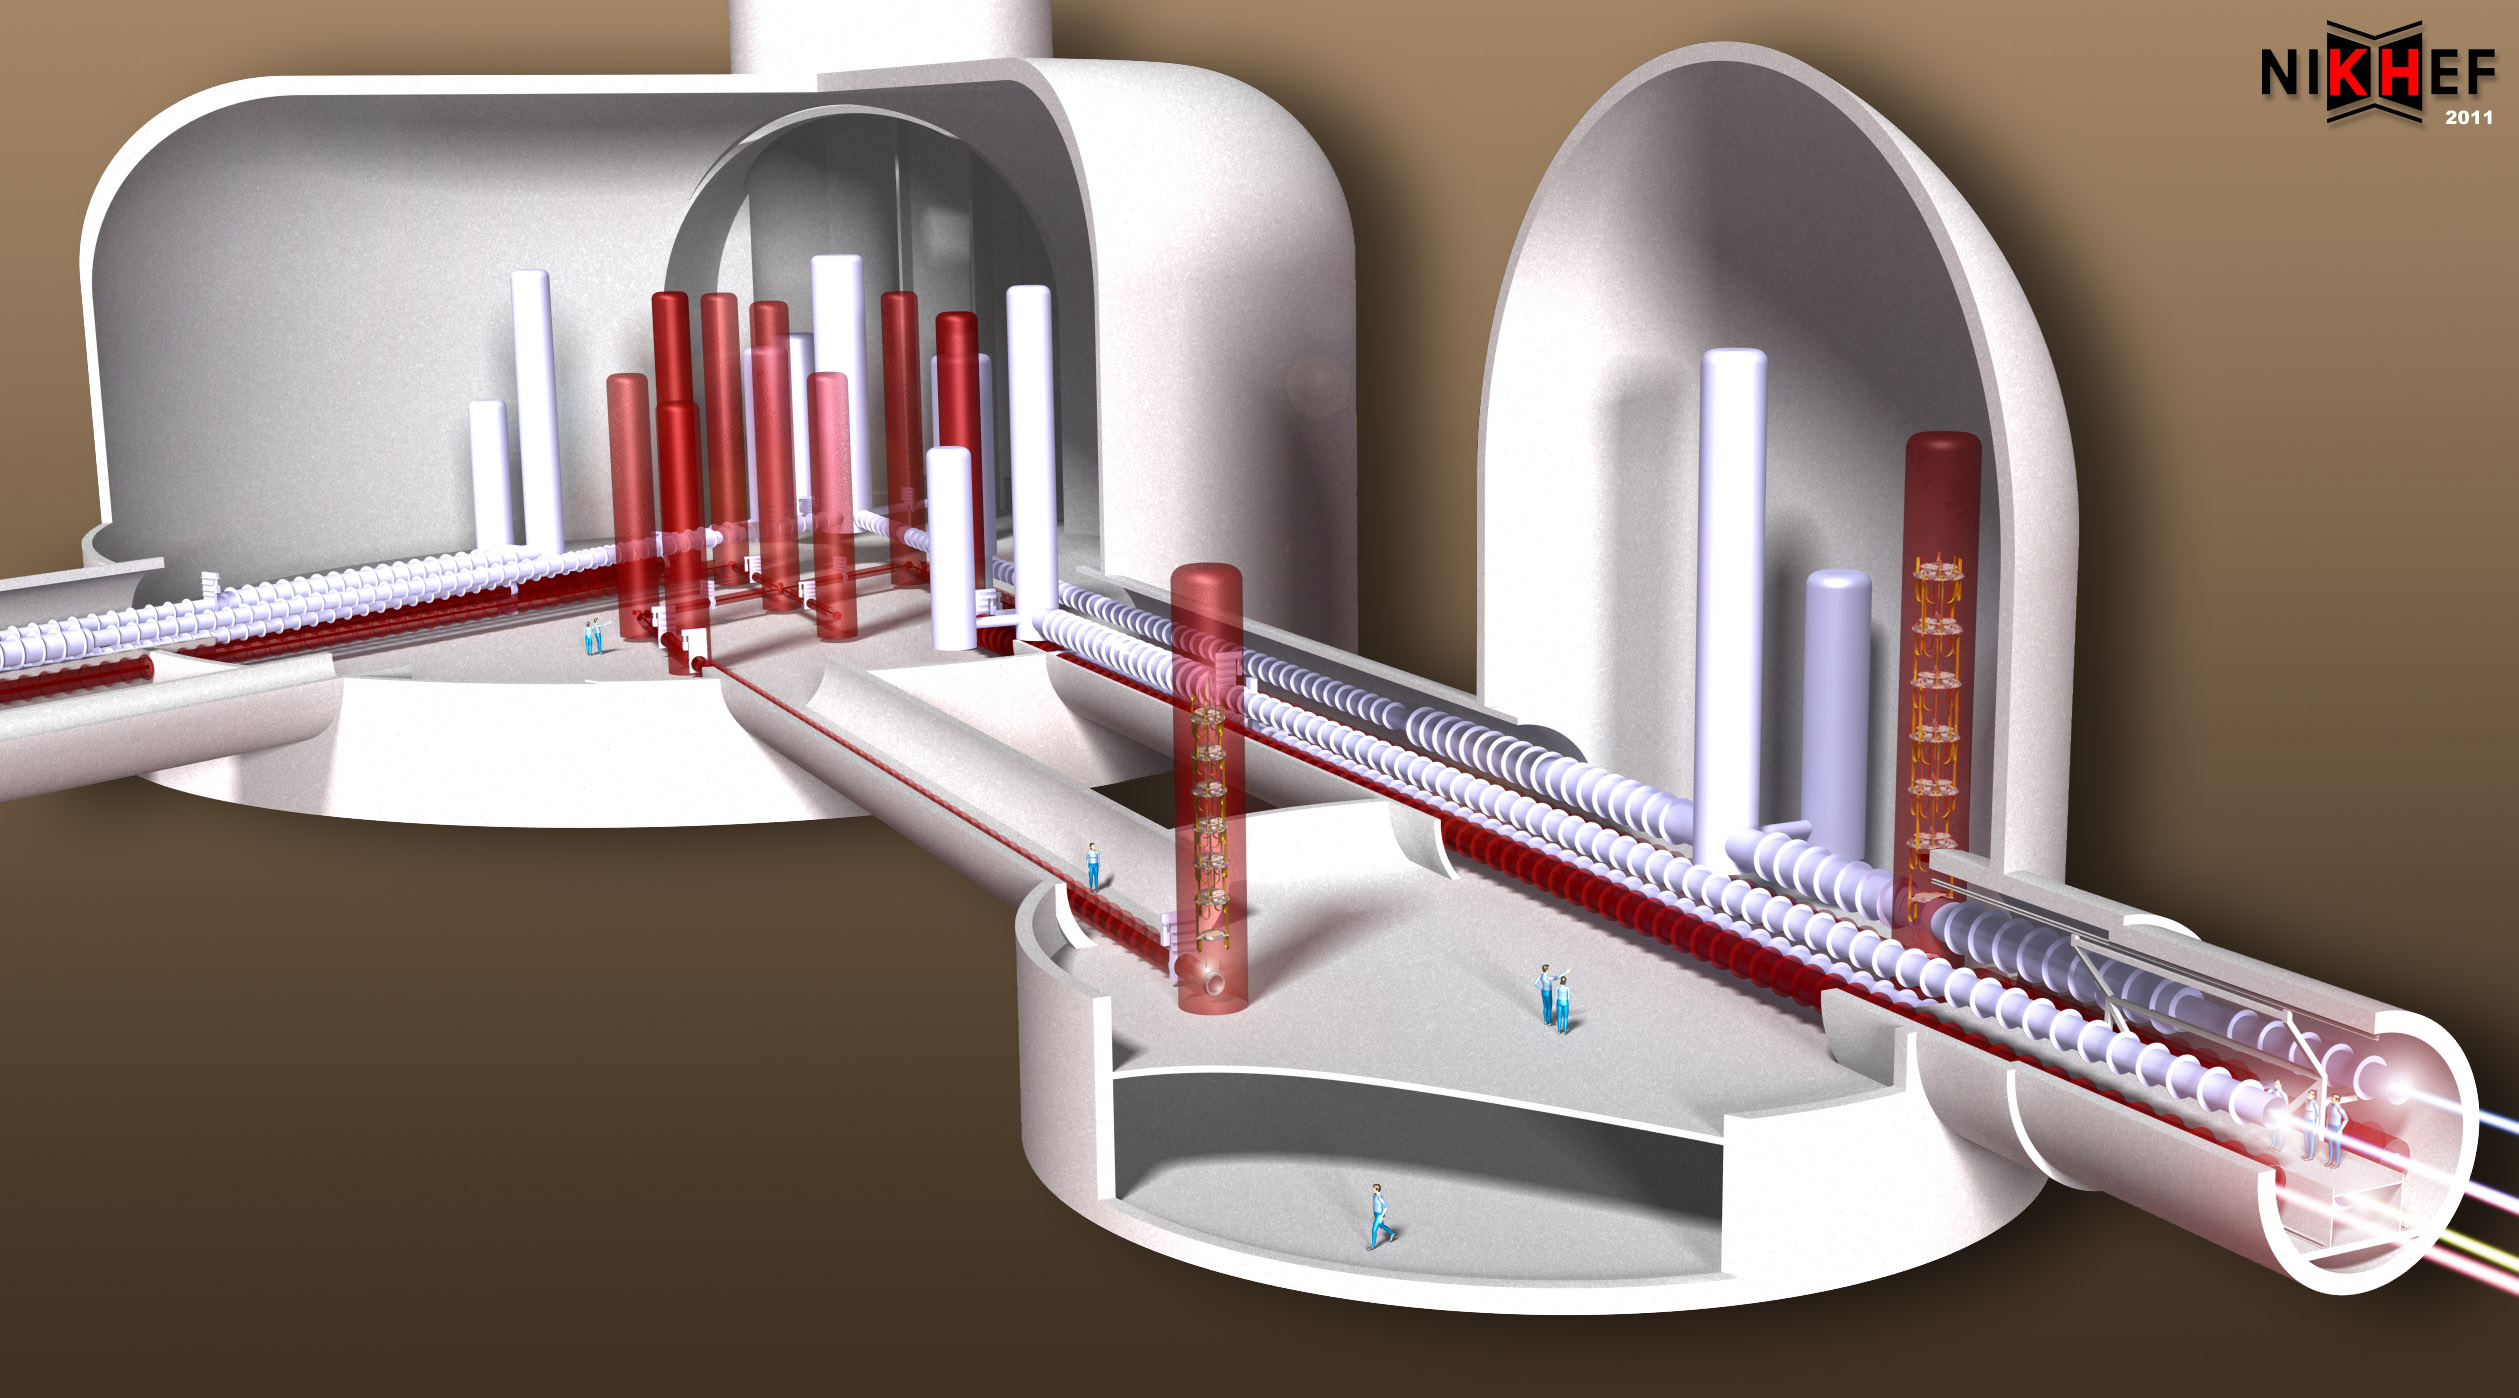
\includegraphics[width=0.66\textwidth]{Sec_SiteInfra/Figures/ArtisticView1.jpg}
	\caption{Artistic impression of the underground arrangement of tunnels and 
	caverns. For details see sections~\ref{subsec:tunnels} and \ref{subsec:caverns}}
	\label{fig:Artisticview1}
\end{wrapfigure}
The main $\simeq$10\,km tunnels that \mbox{connect} two satellite stations (see 
section~\ref{subsec:tunnels}) will have an inner diameter of 5.5\,m, which will \mbox{locally} 
be increased to 6.0\,m wherever the insulation for \mbox{cryogenic} operation requires more 
space. The three {\mbox vertex} caverns and six satellite caverns will house the 
vacuum \mbox{vessels} and must be about 25\,m high (see section \ref{subsec:caverns}). 
Access to the \mbox{underground} detectors is foreseen via vertical shafts (see 
figure~\ref{fig:infra}). It remains to be explored in a technical design phase after site 
selection whether horizontal access is favourable. This option may, for instance, be 
advantageous if the \mbox{Observatory} is built inside a mountain. 

The ET infrastructure will house the observatory for many decades, during which 
the interferometers will receive upgrades as technology advances. Some of these 
changes may result in the necessity to change mirror positions and with it vacuum 
tank positions as we now see in the upgrades from the `initial' to the `advanced' 
generation of gravitational wave detectors. Hence we plan to build large caverns 
where the tanks can be placed at arbitrary positions, instead of building an inflexible 
system of short tunnels connecting narrow but tall caverns housing a single vacuum 
tank each.  

Above ground, at the entrance to the vertical axis shafts, facilities housing workshops, 
offices, apartments, technical facilities providing cryogenic fluids, air conditioning 
and venting, emergency electricity generators, etc.\ will be set up, as shown in figure 
\ref{fig:infra}. 
One major aspect of the design of the total infrastructure is to provide an environment 
able to house not only the basic initial version of the Einstein telescope that we 
describe in this Design Study document but also be versatile enough to accommodate 
upgraded versions in the following decades to come.   
\FloatBarrier
\subsection{Observatory timeline}
%\emph{Authors: M.Punturo, H. Lueck} \\
The realization of the ET observatory will be the final step of a long path and the initial 
act of a new scientific adventure. Several steps have been necessary (see 
Sec.~\ref{TimelineSubSection}) to allow the realization of this conceptual design study 
document  and few other important achievements are needed to reach the readiness 
condition for the observatory realization. The design of the new detector must evolve 
from the current conceptual phase to the technical design phase, successful R\&D 
activities must confirm the feasibility of the solutions proposed in this document, but, 
first of all, it is crucial that advanced detectors confirm the effectiveness of their new 
technologies and that a gravitational wave signal is detected in these interferometers. 
The detection of gravitational waves is regarded as a prerequisite for the start of 
construction of the Einstein Telescope.
For this reason the excavation of the ET site cannot start before 2017, and hence 2018 
is here taken as the initial time ($t_0$) for the ET observatory realization. ET being 
an observatory that will be \emph{on line} for decades, priority in construction 
will be attributed to the site and infrastructures realization, selecting a modular 
philosophy for the detectors that will allow to implement the different interferometers 
composing each detector with a schedule stretched in time. In this way, after about 6 
years of construction, installation and commissioning, the first detector of the ET 
observatory could be operative at the end of the first half of the next decade.
\FloatBarrier
\subsection{Observatory costs}
%\emph{Authors: M.Punturo, H. Lueck} \\
At this stage of the conceptual design the costs of the Observatory have to be regarded 
as a rough estimate. A summary of the estimated costs is shown in 
figure~\ref{Fig:TotalCostTable}. More details on the costing are explained in 
section~\ref{ConclusionsCostsSubSection}. 
The overall costs of an underground facility like the Einstein Telescope Observatory 
are dominated by excavation costs and construction of the underground tunnels and 
caverns. These costs depend significantly on the location and type of soil. In this 
design study a rather conservative assumption of 260\,\texteuro$\rm{/m^3}$  has been 
made. The costs listed in the figure~\ref{Fig:TotalCostTable} assume a single detector 
to be implemented first. The costs include spares for each individual item. In most 
instances the spares will remain unused and can act as spares for the subsequent 
installation of the other two detectors, reducing their price tags somewhat.

%
\cleardoublepage
\FloatBarrier
\begin{textblock*}{297mm}(0mm,0mm)   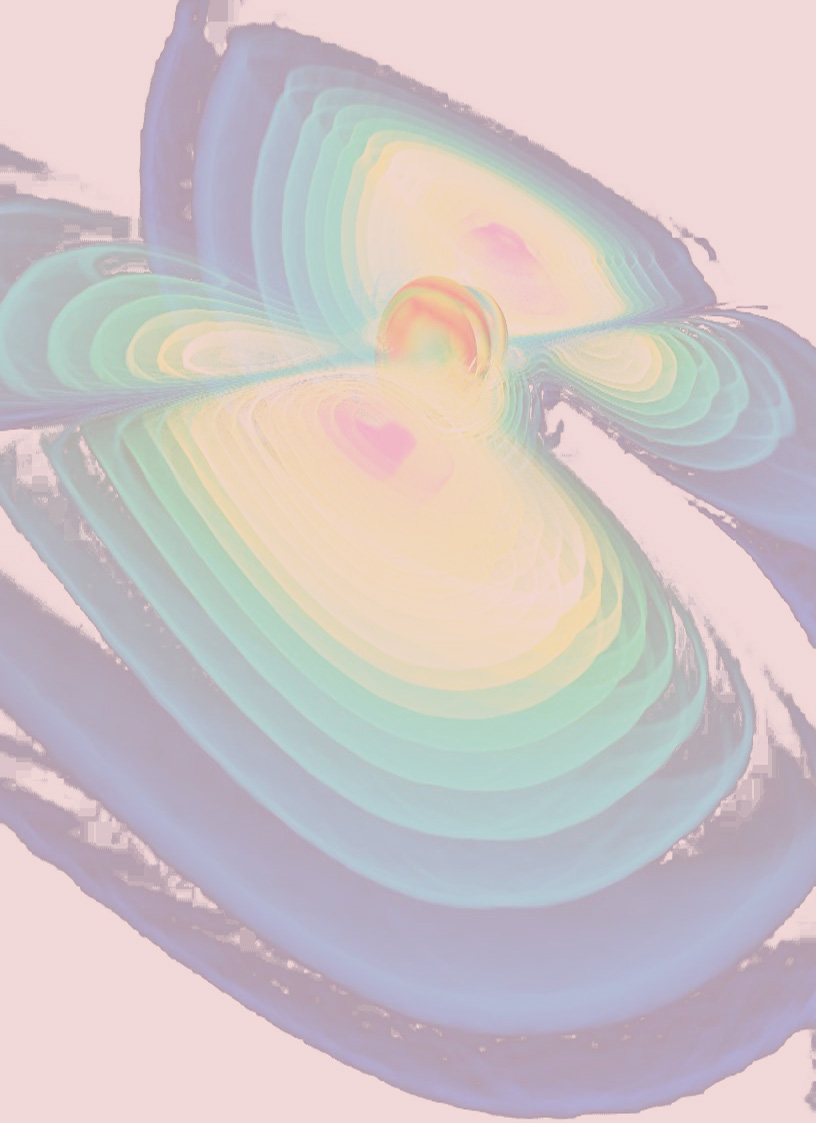
\includegraphics[width=\paperwidth]{Sec_ET_ScienceCase/BackgroundFirstPageScienceCase.jpg}
\end{textblock*}
\section{Science case}
\def\gsim{\mathrel{
\rlap{\raise 0.511ex \hbox{$>$}}{\lower 0.511ex
\hbox{$\sim$}}}}
\def\lsim{\mathrel{
\rlap{\raise 0.511ex \hbox{$<$}}{\lower 0.511ex
\hbox{$\sim$}}}}

\FloatBarrier
\subsection{Introduction}
Some three hundred years after Galileo observed the Jovian
satellites, the twentieth century heralded a new era in
observational astronomy with  radio and microwave antennas and
gamma- and X-ray detectors, which revolutionized astronomy and
opened the entire electromagnetic spectrum for observing
and understanding the Universe. Each new spectral window
has unveiled a new source or phenomenon that could not have been
discovered in any other way. A remarkable revelation
coming from these observations is that about 96 percent of
our Universe is invisible and that gravitational interaction
powers the most luminous and spectacular objects and phenomena
such as quasars, gamma-ray bursts, ultra luminous X-ray sources,
pulsars, and the evolution of the early Universe. Gravity has,
so far, played a passive role. But that is about to change.

Einstein's General Theory of Relativity is among the most 
successful physical theories of the 20th century. It has
passed with flying colours all laboratory-based experiments
and solar system tests.  It predicts that dynamical systems 
in strong gravitational fields will release vast amounts of 
energy in the form of gravitational radiation (see Box 
\ref{box:gw} for a brief introduction to gravitational waves).
This radiation has the potential to open a new window on the Universe, 
complementing the electromagnetic window. Russell Hulse 
and Joseph Taylor were awarded the 1993 Nobel Prize in Physics for 
their discovery of a binary consisting of two neutron stars in 
close orbit, in which indirect evidence for the emission of
gravitational waves (GWs) was found. 

\FloatBarrier
\subsection{Executive Summary}
Gravitational waves interact weakly with matter because gravity 
itself is very weak.  Detectable amounts of gravitational 
radiation cannot be produced in a laboratory but catastrophic 
astronomical events could be the source of strong GWs.
The first attempts to detect cosmic gravitational radiation were made in 
the 60's by Joseph Weber, who built resonant bar detectors, but they were 
not sensitive enough to even the most energetic sources of gravitational 
waves, such as a nearby supernova.  Over the past four 
decades, progress in technology has led to the construction of 
ever more sensitive instruments, culminating in long-baseline
laser interferometric detectors such as the
European GEO\,600 and Virgo and the American LIGO.

Interferometric detectors that are currently
taking data, and advanced detectors that will be built over the next 
five to ten years, will be the first steps in establishing the field of 
{\em gravitational astronomy.} Advanced Virgo and LIGO are expected 
to observe several tens of inspiralling and merging binaries of 
neutron stars (NSs) and black holes (BHs) each year. They could also detect 
occasional Galactic sources such as transients associated with supernovae, 
glitching pulsars, or soft gamma-ray bursts.
This phase of observation will, for the first time, test 
Einstein's theory in the dissipative regime beyond the basic quadrupole 
approximation, verify the existence of binary black holes (BBHs), measure the 
speed of gravitational radiation relative to the speed of light and map 
the expansion rate of the Universe on scales of hundreds of megaparsec (Mpc), 
providing a completely independent estimate of the Hubble parameter. 

Advanced Virgo and LIGO will be sensitive to binary neutron stars (BNSs)
at a distance of 200\,Mpc and to stellar mass BBHs
at a red shift of $z=0.5.$ The lower frequency cutoff of a detector 
places an upper limit on the total mass of binary systems they can 
detect. A lower frequency cutoff of 20\,Hz in the case of Virgo and LIGO
limits the total mass to be less than about $200\,M_\odot.$ 
ET plans to improve the amplitude sensitivity by an order of magnitude 
and extend the frequency sensitivity down to 1\,Hz. This will allow
astronomers to explore binaries at cosmological distances and
unveil new sources: ET would observe BNS
up to a redshift of $z\sim 2,$ stellar-mass BBH
population at the edge of the Universe ($z\sim 15$) and 
intermediate-mass ($10^2$--$10^4\,M_\odot$) BBH out to a typical
redshift limit $z\sim 5$. ET will be sensitive to supernovae out to a
distance of 15 million light years within which one might expect to
observe an event every year. 

An observatory with the capability of ET will produce tremendous scientific 
payoffs.  ET will make it possible to observe a greater variety of 
phenomena and provide a new tool for expanding our knowledge of fundamental
physics, cosmology and relativistic astrophysics. ET's key science
objectives are:

\paragraph {\bf Fundamental Physics and Gravity}
\begin{enumerate}
\item {\em Is the nature of gravitational radiation as predicted by 
Einstein's theory? }

ET will allow a test of the wave generation formula beyond the quadrupole 
approximation and check whether 
there are only two polarizations as predicted by Einstein's theory or six as 
in scalar tensor theories. It could accurately measure the GW propagation 
speed by coincident observation of GW and EM radiation from BNS
coalescences at $z\sim 2$ and constrain the graviton mass.

\item {\em Are black hole spacetimes uniquely given by the Kerr geometry?}

By measuring different quasi-normal modes, ET will test if 
the spacetime geometry of a BH is uniquely described by its mass and spin.
% \footnote{Although astronomical black holes could have electric charge 
% it is expected that any residual charge would be quickly neutralized.} 
Additionally, ET can measure the multipole moments of a source from the 
radiation emitted as a stellar-mass BH spirals into an 
intermediate-mass BH and confirm if the different moments 
depend only on the massive BH's mass and spin.

\item {\em What is the physics of gravitational collapse?}

ET can study supernovae and explore if they leave behind a massive 
object that is trapped inside an event horizon or lead to a naked 
singularity, or some other exotic object. ET could well reveal a new 
class of objects and phenomena, for instance \emph{silent supernovae} 
\cite{Woosley:1992} and other gravitationally unstable transients.

\item {\em What is the equation of state of matter at 
supra-nuclear densities as might be found in NS cores?}

The equation of state (EoS) of NSs affects the late-time evolution of 
BNS and neutron star-black hole (NSBH) binaries. By matching the observed 
radiation from the coalescence of such sources to theoretical predictions, ET will 
deduce the EoS of NS cores.

\item {\em What is the maximum mass of a neutron star?}

The maximum mass of a white dwarf is $\sim 1.4\,M_\odot$ as determined 
by the electron degeneracy pressure.  The maximum mass of a NS is an 
additional test of the nature of matter at extremely high densities; 
it is currently unknown and should be determined by accurately
constructing their mass function from millions of BNS systems observable
in ET.

% \item Are there really ten spatial dimensions? 
% \item What is the nature of quantum gravity and what is the origin of space and time? 
\end{enumerate}
\paragraph {\bf Cosmology}
\begin{enumerate}
\item {\em What are the true luminosity distances of cosmological sources?}

BBH and BNS binaries are an astronomer's ideal {\em standard candles}
or, more appropriately, {\em sirens}.
Gravi\-tational wave observations alone can determine both the 
apparent and absolute luminosity of a source. With ET these standard sirens can
be used to calibrate the cosmic distance ladder.

%\item {\em Is the Universe isotropic and does it expand at the same rate in different 
%directions?}

%A precision measurement of the Hubble parameter will allow ET to map the 
%rate of expansion of the Universe in different directions and discover
%tiny anisotropies.

\item {\em What is the EoS of dark energy and how does it vary with redshift?}

ET could observe thousands of coalescing BNS and NSBH
systems in coincidence with optical or gamma-ray observations
and hence measure both the luminosity distance and 
redshift. ET will, therefore, facilitate precision 
measurement of the dark energy EoS and its variation with redshift.

\item {\em How did black holes at galactic nuclei form and evolve?}

ET can verify if seeds of galaxy formation were intermediate BHs
of hundreds to thousands of solar masses and map their merger history up to
redshifts of $z\sim 5$--15 depending on the total mass and mass ratio of 
progenitor binaries.

\item {\em What were the physical conditions in the primeval Universe and what
phase transitions occurred in its early history?}

Stochastic GW backgrounds could be produced by quantum 
processes in the primordial Universe or during phase transitions in its 
early history. ET will be sensitive to background densities $\rho_{\rm GW}
\gsim 10^{-12}\,\rho_c,$ where $\rho_c$ is the critical density of the Universe.

\end{enumerate}

\paragraph {\bf Astrophysics and Multimessenger Astronomy}
\begin{enumerate}
\item {\em What is the mass function of BHs and NSs and
their redshift distribution?}

ET will measure masses and spins of millions of NSs and BHs
in binary systems and will thereby obtain a census of these objects as a function of
redshift. This will be a very valuable database for understanding a host of questions
in astronomy related to redshift evolution of compact objects. 

\item {\em What are the progenitors of gamma-ray bursts?}

Gamma-ray bursts (GRBs) are the most luminous electromagnetic sources in the
Universe. While advanced detectors might provide some clues as to their
origin, ET will provide a large statistical sample of events that
could be used to understand GRB progenitors and to test their astrophysical models. 

\item {\em How do compact binaries form and evolve?}

The process by which main sequence binary stars evolve into compact 
binaries (that is, BNS and BBH)
could be understood by ET's observation of millions of coalescing
binaries with different masses, mass ratios and spins and mapping the
observed population to astrophysical models.

\item {\em What is the physical mechanism behind supernovae and how asymmetric 
is the gravitational collapse that ensues?}

Supernovae are complex processes whose modelling requires many 
different inputs, including relativistic magneto-hydrodynamics, general relativity
and nuclear and particle physics. 
ET's observation of supernovae in coincidence with EM afterglows and 
neutrinos could provide the data necessary to constrain models and help
understand the process by which stars collapse to form NSs and BHs.

\item {\em Do relativistic instabilities occur in young NSs and if so 
what is their role in the evolution of NSs?}

Non-linearities of general relativity could cause instabilities in 
NSs that lead to parametric amplification of GWs.
ET's observations of the formation of NSs can explore if such
instabilities occur in young NSs and how that might affect
their spin frequencies.

\item {\em Why are spin frequencies of NSs in low-mass X-ray binaries bounded?}

ET will verify if gravitational radiation back-reaction torque is responsible 
for the observed upper limit on NS spin frequencies in low-mass X-ray binaries.

\item {\em What is the nature of the NS crust and its interaction 
with the core?}

ET should detect NS ellipticities that are $\rm few \times 10^{-10}$
or larger depending on their spin frequency. This can be used to deduce the
property of NS crusts. ET might also detect GWs 
that are expected to be emitted when pulsars glitch and magnetars flare and thereby
help understand crust-core interaction that is believed to transfer angular 
momentum from the core to crust.

\item {\em What is the population of GW sources at high redshifts?}

A large population of point sources would produce a confusion background that would
be detectable by ET if the energy density of the background is large enough.
Detection of confusion backgrounds can be used to understand the nature and
population of GW sources in the Universe.
\end{enumerate}
%
Gravitational radiation is an essential prediction of any relativistic
theory of gravity. It will be a new tool for observing the most 
energetic processes in the Universe---processes originating
in such extremely dense environs that all other forms of radiation
and particles might be trapped. In this chapter we will look at
what new science is enabled by ET and how its low frequency 
($<10$\,Hz) sensitivity will be critical in achieving its key science objectives. 

\etbox{i}{box:gw}
{Gravitational Waves}
{At a sufficiently large distance from cosmic sources, GWs 
can be described as a small perturbation to a flat spacetime. 
The spacetime can thus be described by a metric
$g_{\alpha\beta}=\eta_{\alpha\beta}+h_{\alpha\beta},$
$|h_{\alpha\beta}|\ll 1,$ where $\eta_{\alpha\beta}={\rm Diag}(-1,1,1,1)$ 
is the flat Minkowski metric and $h_{\alpha\beta}$ is the perturbation 
due to GWs.  In a suitable coordinate system and gauge,
$h_{\alpha\beta}$ has only two independent components conventionally
called the ``plus" and ``cross" polarizations $h_+$ and $h_\times,$ 
respectively: $h_+\equiv h_{xx}=-h_{yy},$ $h_\times \equiv  h_{xy} = 
h_{yx} $, all other components being zero, $h_{0\alpha}=h_{z\alpha}=0.$ 
\\[5pt]
The apparent luminosity of radiation ${\cal F}$, at great distances 
from the source and in geometrical units in which $c=G=1$, is related to the 
time-derivative of the amplitude 
by~\cite{schutz.2009}:
%
\begin{equation}\label{eq:flux}
{\cal F} \sim {| \dot h |^2}/{(16 \pi)}.
\end{equation}
%
If a source at a distance $D$ radiates away energy $E$ in a time $T$, 
predominantly at a frequency $f$, then writing $\dot h= 2\pi f h$ and 
noting that ${\cal F}\sim E/(4\pi D^2T)$, the amplitude of GWs is
%
\begin{equation} \label {eq:amplitude}
h \sim \sqrt{E/T}/(\pi f D) .
\end{equation}
%
Gravitational waves cause a strain in space as they pass. The distance
$L$ between two masses will be altered by an amount $\delta L$ that
is proportional to a linear combination of the two polarizations. 
Figure \ref{fig:pol} below depicts how a ring of free particles responds to
the two polarizations. 
\begin{figure}[H]
\centering
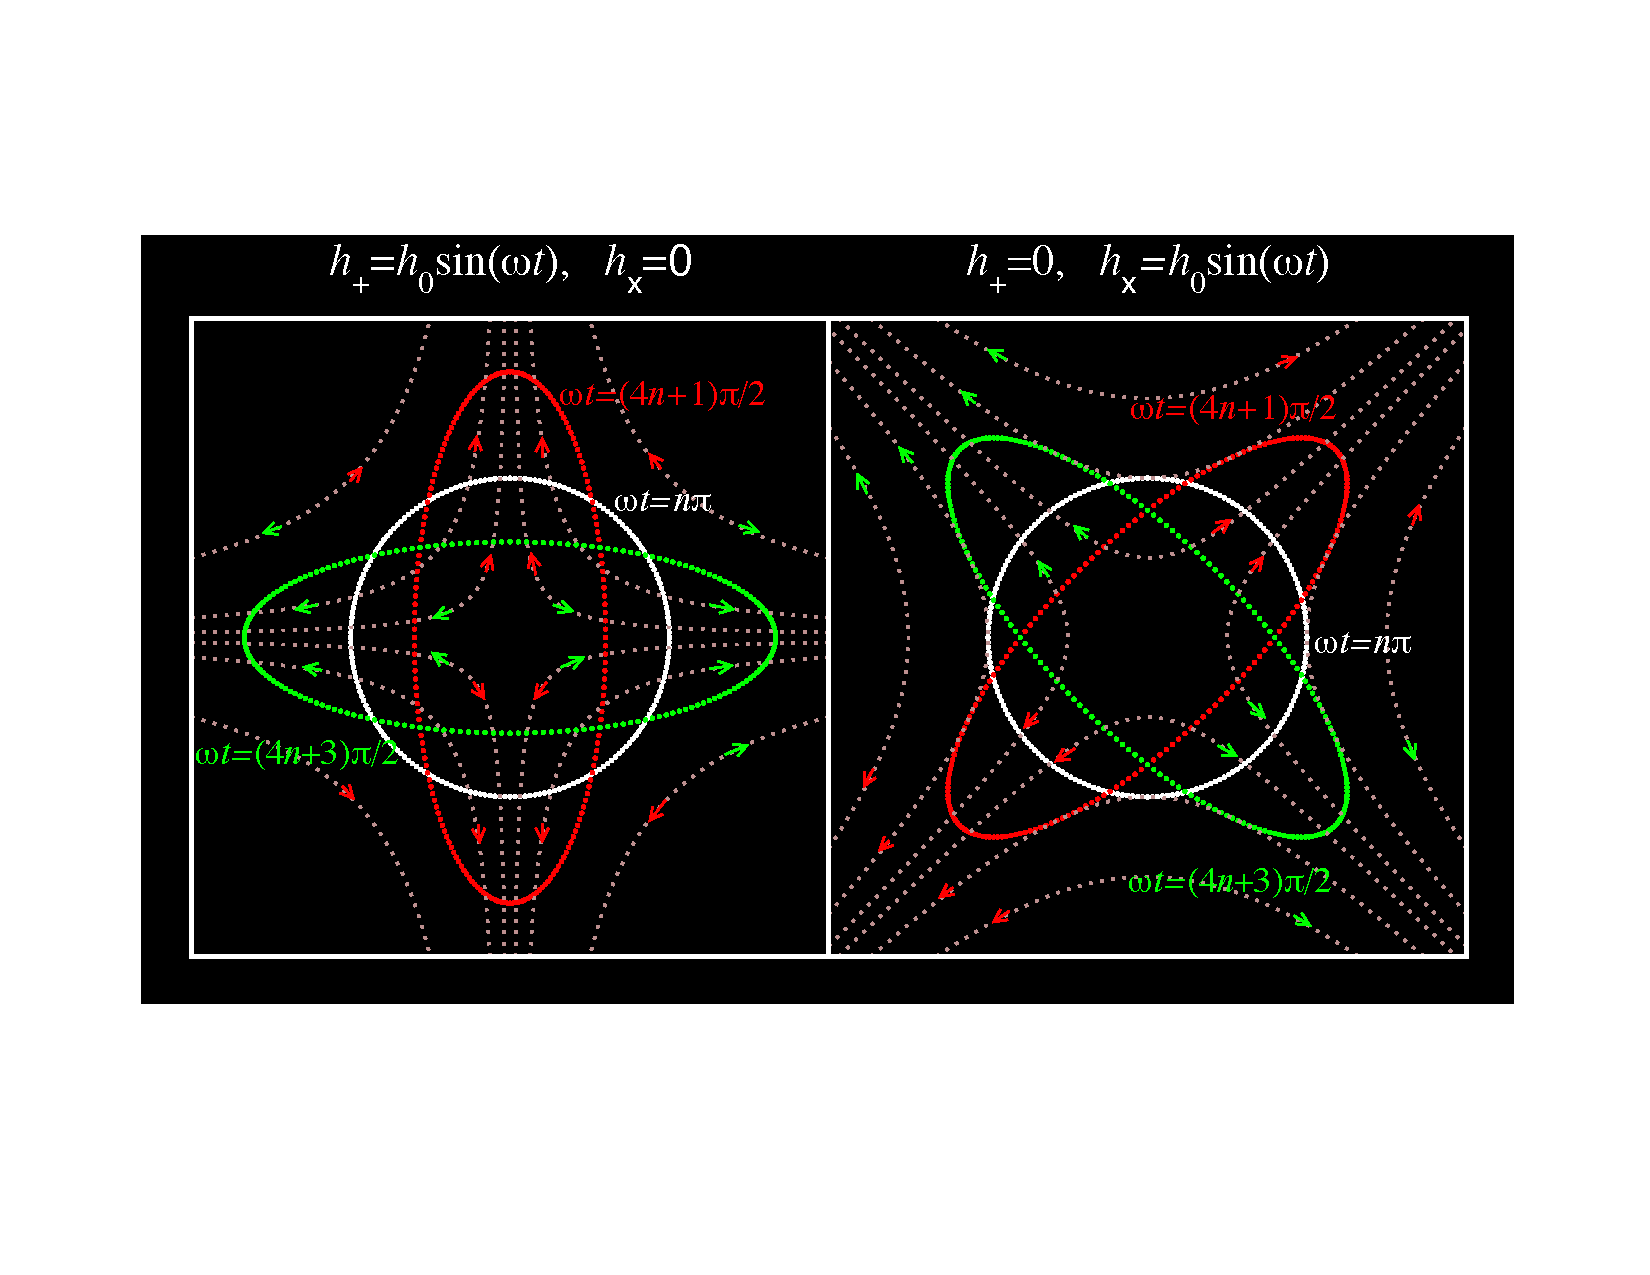
\includegraphics[width=0.95\textwidth]{./Sec_ET_ScienceCase/polarization.pdf}
\vskip 0.3cm
\caption{Response of a circular ring of free particles to a passing sinusoidal 
GW of plus (left) or cross (right) polarization.
The tidal field of the waves on the ring is indicated by light dotted 
lines. The direction of the force reverses sign each half-period of 
the wave as indicated by the red  and green arrows. The ring oscillates between
the red and green ellipses over one period of the wave, the maximum 
eccentricity of the ellipses being the wave amplitude $h_+$ or $h_\times$. 
A general wave is a linear combination of the two polarizations.
}
\label{fig:pol}
\end{figure}
\vskip -0.6cm
A sinusoidal wave incident perpendicular to the plane of the ring tidally 
deforms it into an ellipse over the first quarter of the wave's period, back 
to the ring over the next quarter, to an ellipse oriented orthogonally to the 
first over the third quarter, and back to the ring over the fourth quarter. 
}

\clearpage 

\subsection{Sources of gravitational waves in ET}

The goal of this Section is to give an overview of the sources
expected to be observed by ET and the problems that were addressed 
in the context of the Design Study. A brief description of how ET 
responds to an incident GW is given in Box~\ref{box:response}.
ET will observe GWs from a variety of different astronomical 
sources such as BNSs, BBHs, supernovae, spinning NSs,
glitching pulsars, flaring magnetars, and, perhaps, a primordial 
stochastic background.
We will first give a brief introduction to the types of sources
expected to be routinely observed by ET. This will be followed
by a discussion of the fundamental physics, 
astrophysics and cosmology enabled by ET. Recent reviews on sources
and science can be found in Sathyaprakash and Schutz \cite{lrr-2009-2}
and Andersson et al \cite{2011GReGr..43..409A}.

\etbox{i}{box:response}
{ET's Response to Gravitational Waves}
{
A single interferometric gravitational-wave detector cannot 
measure both polarizations of GW, but only a linear combination of the
two, called the \emph{response} $h(t)$, given by
\begin{equation}
h(t) = F_+(\theta,\, \varphi,\, \psi) h_+(t) +
       F_\times(\theta,\, \varphi,\, \psi) h_\times(t).
\label{eq:response}
\end{equation}
Here, $F_+$ and $F_\times$ are the detector antenna pattern functions,
$\psi$ is the polarization angle, and $(\theta,\,\varphi)$ are angles
describing the location of the source on the sky (see \emph{e.g.}\ 
Ref.~\cite{lrr-2009-2} for details). The various angles can be treated as
constants for transient sources, but must be taken to be 
time-dependent for sources that last for more than about 30 min, after
which Doppler modulation of the signal due to the relative motion 
of the source and detector cannot be neglected.
\\[5pt]
It is expedient to write the response as
\begin{equation}
h(t)=F(t)\left(\cos\xi\,h_+ + \sin\xi\,h_\times\right),\quad
F=\sqrt{F_+^2+F_\times^2},\quad \tan\xi=F_\times/F_+.
\end{equation}
It turns out that $F$ is independent of the polarization angle and
so measures the sensitivity of the detector to different locations on
the sky.  Figure \ref{fig:response} below plots $F(\theta,\,\varphi)$
for an L-shaped interferometer such as Virgo (panel on the left) 
and for a triangular ET (panel on the right). Since ET consists of 
a triangle of three detectors, it is a factor $\sqrt{3}$ more sensitive 
than a single detector; but, since the opening angles of the 
arms are $\pi/3,$ the sensitivity is smaller by a factor $\sin (\pi/3)= \sqrt{3}/2$ 
compared to an L-shaped detector---an overall factor of 3/2, as 
can be seen in Fig.~\ref{fig:response}.
\begin{figure}[H]
\centering
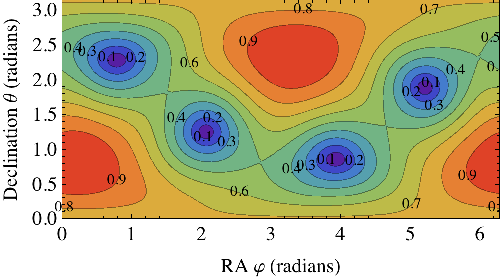
\includegraphics[width=0.495\textwidth]{./Sec_ET_ScienceCase/Virgo-AP.pdf}
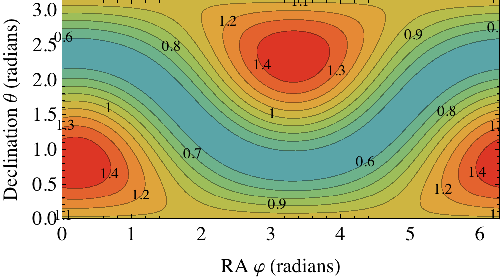
\includegraphics[width=0.495\textwidth]{./Sec_ET_ScienceCase/ET-AP.pdf}
\vskip 0.3cm
\caption{Antenna pattern of ET (right panel) compared to that of
Virgo (left panel). ET is assumed to be at the same location as
Virgo. Note that Virgo is a {\em single} L-shaped detector while
ET consists of {\em three} V-shaped interferometers rotated relative 
to one other by 120 $\deg.$ The combined antenna pattern of the three detectors 
in ET (defined as $F^2=\sum_{A=1}^3\,F_A^2$, where $F_1,F_2,F_3$ are the
individual antenna pattern functions) makes the response the same for all 
sources whose sky location makes the same angle to the plane formed 
by ET (see \emph{e.g.}\ contours marked 0.6).}
\vskip -0.3cm
\label{fig:response}
\end{figure}
}
\subsubsection{Compact binary coalescences}
\label{sec:binaries}

\begin{figure*}
\centering
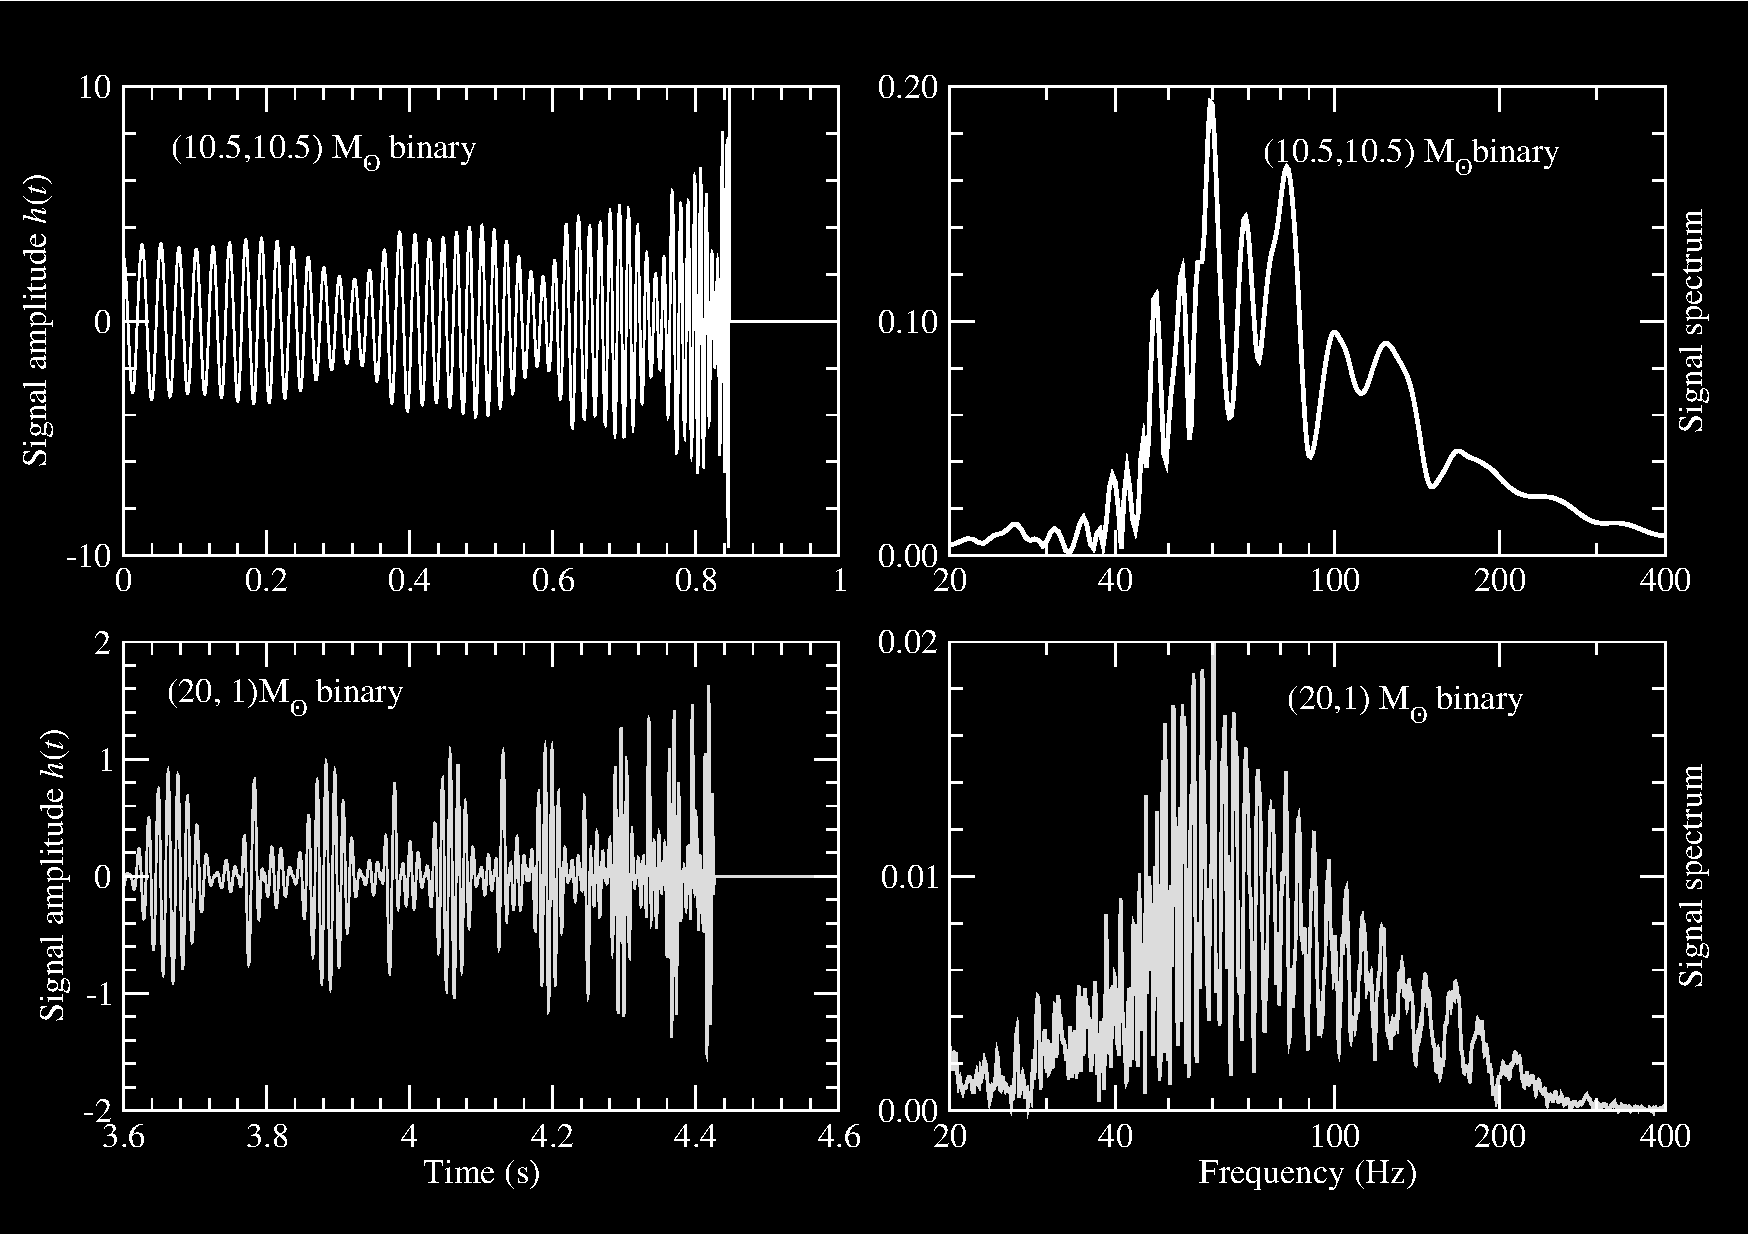
\includegraphics[width=0.99\textwidth]{./Sec_ET_ScienceCase/spinningBinaries.pdf}
\caption{The waveforms from two compact binary systems that ET could
detect. Left panels show the time-domain waveforms (for clarity only the
last second is plotted), right panels show the frequency spectrum. 
The upper two panels show a binary composed of two equal masses; the 
waveform's modulation is due to interaction between the spins of the bodies 
and the orbital angular momentum. The lower panels show a binary 
composed of a neutron star and a black hole. In this case, the signal 
amplitude is smaller, the duration is longer due to the larger mass ratio, 
and the signal modulation is stronger as the spin-orbit precession of the 
orbital plane is greater.}
\label{fig:chirps}
\end{figure*}

A compact binary, consisting of NSs and/or BHs,
evolves by emitting gravitational radiation which extracts rotational energy 
and angular momentum from the system. This causes the two bodies to
inspiral toward each other and eventually merge. The dynamics of a compact 
binary can be described in three phases:
\begin{itemize}
 \item The \emph{inspiral phase} in which the
system spends hundreds of millions of years. During this phase the luminosity
in GW is low and the dynamics can be solved using approximation
methods --- the most popular being the post-Newtonian (PN) approximation
(see Box~\ref{box:pn}). The two polarizations are given at the lowest order
approximation by Equations (\ref{eq:amps}), Box \ref{box:pn}. At the dominant
PN order, the frequency of the emitted signal is twice the orbital frequency;
the signal has a characteristic shape, with slowly increasing amplitude and 
frequency, called a \emph{chirp} waveform. A BNS system will stay in
ET's sensitivity band for nearly a week starting from 1\,Hz, 20 hours starting from
2\,Hz, and a little less than 2 hours starting from 5\,Hz. For the same lower frequency 
limits the duration of a BBH signal from a pair of 10$\,M_\odot$ BHs is 2 days, 
45 minutes and 4 minutes, respectively. Such long durations, owing primarily 
to the low frequency sensitivity of ET, are crucial in obtaining very accurate 
estimates of a binary system's parameters, which is essential to achieve some 
of the scientific goals of ET.

When the binary companions are spinning, the signal is modulated due to 
spin-orbit and spin-spin couplings as in Fig.\ \ref{fig:chirps}. These modulations
encode the parameters of sources (their masses, spins, inclination of the orbit,
etc.) most of which can be extracted very accurately 
\cite{Arun:2005,Vecchio:2003tn,vanderSluys:2008qx,Lang:1900bz} by matching 
the observed signals onto general relativistic predictions.

At higher PN orders, the signal also contains other harmonics of the orbital
frequency and including these in the estimation of parameters has proved to
be extremely important, especially for localizing the source on the sky
\cite{VanDenBroeck:2006ar,Broeck2007,Arun:2007hu}.


\etbox{i}{box:pn}
{Post-Newtonian Description of the Inspiral Signal}
{
The adiabatic evolution of a compact binary, during which the
emission of GWs causes the component stars
of the system to \emph{slowly} spiral in towards each other,
can be computed very accurately using the 
PN expansion of the Einstein equations. Currently, the
dissipative dynamics is known  to order
$(v^7/c^7),$ where $v$ is the characteristic velocity in
the system.
\\[5pt]%\indent
For a binary consisting of two stars of masses $m_1$ and
$m_2$ (total mass $M\equiv m_1+m_2$ and symmetric mass ratio
$\nu\equiv m_1m_2/M^2$), at a luminosity distance $D_{\rm L}$,
the dominant parts of the two polarizations are given by
%%\begin{widetext}
\begin{subequations}
\label{eq:amps}
\begin{align}
h_+(t) & = \frac{2\nu M}{D_{\rm L}}(1 + \cos^2\iota)
\left [M\omega(t;t_0,M,\nu) \right ]^{\frac{2}{3}} \cos \left [2\Phi(t; t_0, M,\nu) + \Phi_0 \right ],\\
h_\times(t) & = \frac{2\nu M}{D_{\rm L}}2\cos\iota\,
\left [M\omega(t;t_0,M,\nu) \right ]^{\frac{2}{3}} \sin \left [2\Phi(t;t_0, M,\nu) + \Phi_0 \right ],
\end{align}
\end{subequations}
%%\end{widetext}
where $\iota$ is the angle of inclination of the binary's orbital angular
momentum with the line-of-sight, $\omega(t)$ is the angular velocity
of the equivalent one-body system around the binary's centre-of-mass and
$\Phi(t;\, t_0,M,\nu)$ is the corresponding orbital phase. Parameters
$t_0$ and $\Phi_0$ are constants giving the epoch of merger and the
orbital phase of the binary at that epoch, respectively.
The orbital dynamics, and hence the phase $\Phi,$ are known to order
$(v^7/c^7)$.
% where $v$ is the characteristic velocity in the system. 
\\[5pt]\indent
The above expressions for $h_+$ and $h_\times$ contain only the dominant
terms which oscillate at twice the orbital frequency. Higher order amplitude
corrections contain other harmonics (\emph{i.e.}\  phase terms depending on
$k\,\Phi(t),$ $k=1,3,4,\ldots$). 
The above expressions are
written down for a system consisting of non-spinning components on a
quasi-circular orbit. In reality, we can assume neither to be
true. Waveforms for binaries on an eccentric inspiral orbit are
known, as are those with spin effects, but we shall not discuss them here.
\vskip 0.2cm
}

\item The \emph{merger} phase when the two stars are moving at around
a third of the speed of light and experiencing extreme gravitational fields.
A post-Newtonian approximation is not accurate when the two stars get close to
each other. To predict the dynamics of the bodies during this
phase requires the full non-linear structure of Einstein's equations,
as the problem involves strong relativistic gravity and tidal deformation
and disruption.  The merger signal lasts for a very short duration (milliseconds
in the case of stellar mass BHs, to seconds in the case of the
heaviest systems ET is likely to detect). Yet BBH have the greatest 
possible luminosity of all sources one can conjure up, exceeding the 
luminosity of the entire Universe in EM radiation in that short duration.

Numerical simulations of BBH mergers have been highly successful, and 
analytical and phenomenological models of the merger dynamics have been developed. 
Following breakthroughs in 2005 \cite{Pretorius05,Campanelli:2005dd,Baker:2005vv},
it is now possible to numerically solve the full Einstein equations for the 
last orbits that include the merger and ringdown phases, for coalescing BBH
systems with comparable component masses, and to calculate the
GW signal emitted. Subsequent dramatic progress has led both to
simulations of increasing numerical accuracy and physical
fidelity, and to the inclusion of larger numbers of GW cycles before
merger, allowing full GR waveforms to be in principle useful in searching for
BBHs of ever lower mass (see \emph{e.g.}\ Fig.~3 in~\cite{Hannam:2009rd}).

Currently efforts are focussed 
on understanding the full parameter space of BBHs
of arbitrary spins and mass ratios.  In the case of BNSs the 
merger phase is not well understood, as it is complicated by a number of unknown
physical effects, such as the EoS of NSs and their magnetic fields.

 \item The \emph{ringdown} phase when the
two systems have merged to form either a NS or BH, settling down to a
quiescent state by radiating the deformations inherited during the merger.
The emitted radiation can be computed using perturbation theory and
it consists of a superposition of quasi-normal modes of the compact object
that forms after merger. These modes carry a unique signature that depends
only on the mass and spin angular momentum in the case of BH, but depends 
also on the EoS of the supra-nuclear matter in the case of NS. Just as in the
merger phase, here too the signal lasts for a very short duration (of 
milliseconds to seconds depending on the mass of the final object) and 
consistst of two to three cycles. However, the superposition of different modes 
means that the signal can have an interesting and characteristic structure.
\end{itemize}


The merger and ringdown parts of the signal last only for a short duration yet carry
tremendous luminosity. Their inclusion in a matched filter search for binary systems  
dramatically increases the distance reach of ET, relative to the reach obtained with the
inspiral phase alone. As we shall see below, having observational access to
these later stages of the coalescence process will lead to key insights into the 
structure of NS; in the case of BH it will open up the possibility of testing gravity 
in genuinely strong-field dynamics of spacetime.

\begin{figure*}
\centering
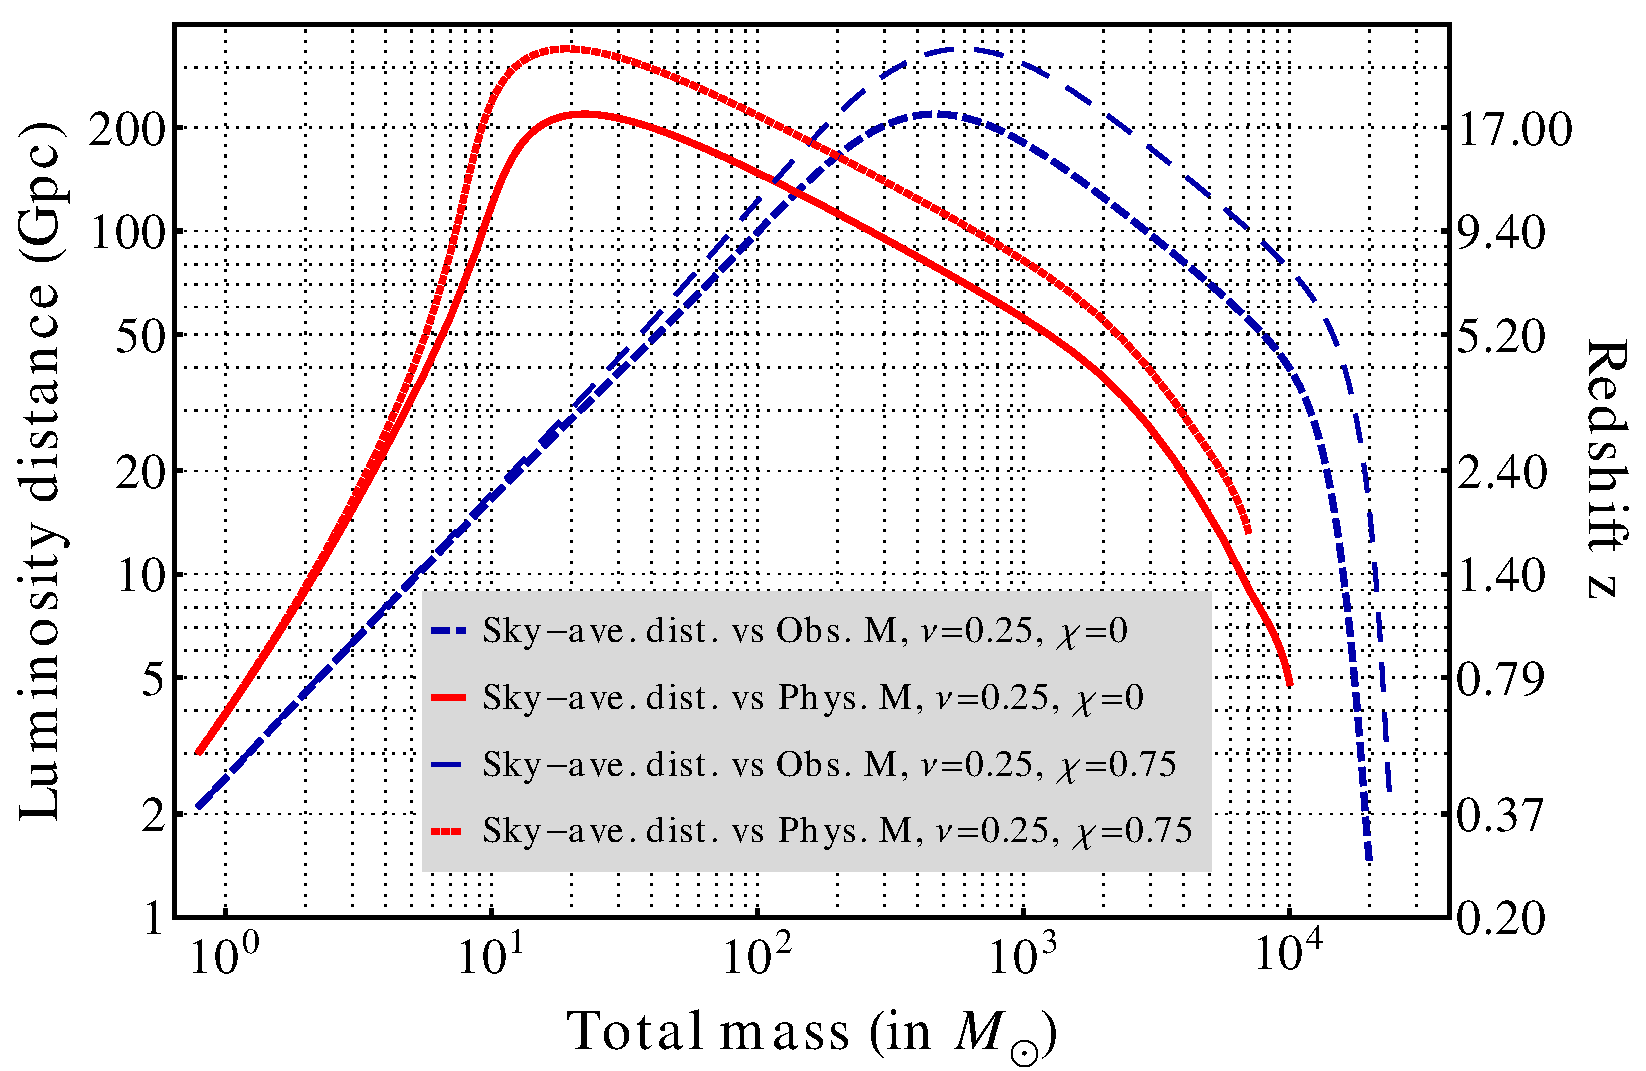
\includegraphics[width=0.75\textwidth]{./Sec_ET_ScienceCase/ET_horDist_ETB.pdf}
\caption{
ET's distance reach for signals from coalescing compact binaries as a function 
of the \emph{intrinsic} (red curves) and \emph{observed} (blue curves) total mass,
averaged over sky position and binary's orientation relative to the line-of-sight.
We assume that a source is visible if it produces an SNR of at least 8 in ET. 
Solid red and short-dashed blue curves correspond to binaries composed of 
non-spinning objects. Dotted red and long-dashed blue curves
correspond to binaries composed of objects whose spins are aligned
with the orbital angular momentum of the binary, with spin parameter $\chi=0.75$.}
\label{fig:ET_range}
\end{figure*}

\paragraph{ET's distance reach and mass range}
A standard measure of the reach of a detector is the horizon distance
$D_h$, defined as the distance at which a detector measures an SNR of 8
for an optimally-oriented and optimally-located binary, \emph{i.e.}\ overhead
from the detector and with a face-on orbit. Sub-optimally located and 
oriented sources are detected with an SNR of 8 at closer distances.

The sky-position averaged distance up to which a 3-detector ET 
observatory would detect signals from coalescing binaries with 
an SNR of 8 is shown in Fig.~\ref{fig:ET_range}, for the ET-B sensitivity 
curve (see Box\,\ref{ETSensitivityCurves}). 
The range is plotted both as a function of the intrinsic (red lines)
and observed (blue lines) total mass. The two are related by the
redshift function $z(D_{\rm L})$ as we will describe later.
The binary systems are modeled by
the phenomenological waveforms of~\cite{Santamaria:2010yb} which
comprise the inspiral, merger and ringdown stages of the coalescence.
Fig.~\ref{fig:ET_range} shows the reach associated
with two physical configurations of the
binary: equal-mass, non-spinning and equal-mass, spin-aligned configuration 
with spins $\chi_1=\chi_2=\chi=0.75$.

A neutron star binary composed of two $1.4\,M_\odot$ NSs would be 
observed by ET from a redshift of $z\simeq 2$. A NS-BH
system comprising a $1.4\,M_\odot$ NS and a $10\,M_\odot$ BH
would be observed from $z \simeq 4$. Binaries formed by stellar-mass BH
will be visible at much larger distances, allowing ET to explore their populations
at cosmological distances of $z\simeq 10$ and further. ET is also sensitive to
intermediate-mass BBHs of total mass in the range [$10^2,\,10^4]M_\odot$
over the redshift range $z\sim1$--15. ET-D's better sensitivity at lower 
frequencies compared to ET-B is important in all cases, but particularly 
so for systems with total mass in the range 500--$10^4\,M_\odot$, for which the
reach is a factor 2--10 greater for ET-D than ET-B.

\begin{table}[ht]
\begin{center}
\caption{
Expected coalescence rates per Mpc$^3$ per Myr in the local universe
($z\simeq 0$).  Also shown are predicted event rates in Advanced LIGO (aLIGO) 
and ET.}
\begin{tabular}{l|ccc}
\hline
\hline
 Source                & BNS              & NS-BH            & BBH            \\
\hline
Rate (Mpc$^{-1}$ Myr$^{-1}$)   &  0.1--6           & 0.01--0.3         & $2\times 10^{-3}$--$0.04$\\
Event Rate (yr$^{-1}$) in aLIGO & 0.4--400          & 0.2--300          & 2--4000          \\
Event Rate (yr$^{-1}$) in ET   & $\mathcal{O}(10^3$--$10^7)$ & $\mathcal{O}(10^3$--$10^7$) & $\mathcal{O}(10^4$--$10^8)$\\
\hline
\hline
\end{tabular}
\label{tab:EventRates}
\end{center}
\end{table}

\paragraph{Expected coalescence rates}
Black holes and neutron stars are expected to form after Type II 
supernovae, which occur roughly once a century in galaxies like our own.  Most stars
seem to form in binaries; a fraction of compact binary progenitors will survive the kicks that
supernovae impart, and roughly half of the remaining low-mass binaries (NSBH, BNS) will 
inspiral and eventually merge through the gradual emission of radiation. With roughly one 
Milky Way-like galaxy per 100\,Mpc$^3$, we anticipate
a rate per comoving volume $\rho_c$ large enough to permit many detections even for advanced
detectors (see Table~\ref{tab:EventRates}).
%  ROS extracts the following from PSellipticals
For example, the binary pulsar population in the Milky Way implies a local BNS merger rate 
$\rho_c^{\rm(NS-NS)}\simeq 0.2-6$\,Myr$^{-1}$\,Mpc$^{-3}$
\cite{Burgay:2003jj,Chunglee-nsns-1,Chunglee-nsns-proceedings}. 
With its vastly greater sensitivity, ET will reach deep back into the universe.
Due to an enhanced star formation rate between $z\simeq 1-3$ \cite{sfr-HopkinsBeacom2006}, 
ET will probe a regime of possibly significantly enhanced compact object merger rates 
\cite{Regimbau:2009,PSellipticals,PSgrbs-popsyn}.
We give an illustration of this for BNS systems in Appendix \ref{box:nsrateestimate}.

Lacking direct observational input, predictions for BBH and NSBH merger 
rates rely entirely on theory. However, recent observational evidence for
BBH progenitors (see below) have allowed, for the first time, an astronomical estimate
of BBH rates.

Studies of isolated binary evolution in the Milky 
Way~\cite{StarTrack2,2006AA...459.1001K,PSmoreconstraints,ChrisBH2007} 
and local universe \cite{PSellipticals} lead to expected event rates in 
the ranges shown in Table~\ref{tab:EventRates}, depending on the assumptions 
adopted in the model.
%
As with the BNS rate, the NSBH merger rate is roughly proportional to 
the star formation rate~\cite{PSgrbs-popsyn} and therefore also increases 
substantially with redshift; many detections are expected.

The BBH merger rate is even more uncertain.  First, long expected delays 
between BBH birth and merger imply BH born in the early universe could merge 
now \cite{PSellipticals}.
%
Second, BH masses depend strongly on the metallicity of the gas from which 
the progenitor star forms, low metallicity environments form both more
binaries and binaries that can be detected farther away
\cite{popsyn-MaxMassBH-Chris2009,popsyn-LowMetallicityImpact-Chris2008}.
Even restricting attention to the local universe, low-metallicity environments
should be significantly over-represented in the present-day detection rate
\cite{popsyn-LIGO-SFR-2008}.
For example, the nearby BBH progenitor binaries IC10 X-1 and NGC300 X1 lie in a low
metallicity environment and suggest a high BBH detection rate for initial 
LIGO of 1 per two years, strongly dependent on survey selection effects (see 
\cite{bhrates-Chris-IC10-2008}).
Further, in the early universe, where fewer generations of stars have produced metals, 
massive binaries could form very frequently
\cite{popsyn-LowMetallicityImpact-Chris2008}.
Third, being the most massive compact objects, BH can \emph{mass segregate} in 
interacting protoclusters. If enough protoclusters persist long enough for this 
process to occur, the BBH binary merger rate could be vastly enhanced 
\cite{clusters-2005,2008ApJ...676.1162S, PZMcM}.
%
As a practical matter, theory provides no useful upper bound; the 
local merger rates of stellar mass
BBH are constrained only by existing GW measurements. 


\paragraph{Standard Sirens of Gravity}

Cosmologists have long sought for standard candles that can
work on large distance scales without being dependent on the
lower rungs of the cosmic distance ladder. In 1986, Schutz \cite{Schutz86}
pointed out that gravitational astronomy can
provide such a candle, or, more appropriately, a {\em standard
siren}, in the form of a chirping signal from the coalescence
of compact stars in a binary.
The basic reason for this is that the gravitational-wave
amplitude depends only on the ratio of a certain combination of the
binary masses and the luminosity distance. For chirping signals
observations can measure both the amplitude of the signal and
the masses very accurately and hence infer the luminosity distance.

\etbox{i}{box:lumdistcbc}
{Coalescing Binaries: Self-Calibrating Standard Sirens}
{
The response of ET to a signal from a coalescing binary can be
found by using the two polarizations in Eq.\,(\ref{eq:amps}) in 
Eq.\,(\ref{eq:response}). The resulting expression can then be written as:
\begin{equation}
h(t) = \frac{2\nu M}{D_{\rm eff}}\, \left [ M\omega(t)\right]^{\frac{2}{3}} \cos[2\Phi(t) + \Phi_0'],
\label{eq:response1}
\end{equation}
where $D_{\rm eff}$ is the effective distance to the binary, which
is a combination of the true luminosity distance $D_{\rm L}$ and
the antenna pattern functions $F_+$ and $F_\times$, and $\Phi_0'$ 
is a constant phase involving the various angles:
\begin{equation}
D_{\rm eff} \equiv \frac{D_{\rm L}}{ \left [ F_+^2\, (1+\cos^2\iota)^2 +
       4\, F_\times^2\, \cos^2\iota \right ]^{1/2}}, \quad
\Phi_0' \equiv \Phi_0 + \arctan \left [-\frac{2\, F_\times\cos\iota }{F_+ (1+\cos^2\iota)}\right ].
\label{eq:response2}
\end{equation}
%\\[5pt]
Thus, for non-spinning binaries on a quasi-circular orbit, the signal is 
characterized by nine parameters in all: $(M, \nu, t_0, \Phi_0, \theta, \varphi, \psi, \iota, D_{\rm L})$.
Since the phase $\Phi(t)$ of the signal is known
to a high order in PN theory, matched filtering can be employed to
extract the signal, and in the process accurately measure the two mass
parameters $(M,\, \nu)$ that completely determine the phase evolution, 
and the two fiducial parameters $(t_0,\, \Phi_0)$.
\\[5pt]
The response of a single GW observatory is not 
sufficient to disentangle the luminosity distance from the angular
parameters.  A network of three non-colocated interferometers (say, ET
and two advanced detectors), can measure three independent combinations 
of the polarizations and two time delays, and hence measure the remaining 
five parameters and thereby extract the luminosity distance.
\vskip 0.2cm
}

The detector response depends only upon a
small number of signal parameters, which can all be measured
either directly or indirectly. The signal is insensitive to
the composition of the component stars, and there is
no complicated modelling required of the structure of the
stars or their environments. Consequently, the measurement
of the luminosity distance is precise, except for statistical errors 
whose magnitude depends on the SNR, and systematic
errors due to weak gravitational lensing. We will discuss
the magnitude of these errors later.


Although the inspiral signal from a compact binary is a standard
siren, there is no way of inferring from it the redshift of a source.
The mappings $M \rightarrow (1+z) M$, $\omega \rightarrow \omega/(1+z),$
and $D_{\rm L} \rightarrow (1+z) D_{\rm L}$ for redshifted sources in Eq.~(\ref{eq:amps})
leave the signal invariant.  Note that a source with an intrinsic
(\emph{i.e.}\ physical) total mass $M_{\rm phys}$ at a redshift $z$ will
appear to an observer to be a binary of total mass $M_{\rm obs}
=(1+z)M_{\rm phys}$. One must optically identify the host galaxy 
to measure its redshift. Thus, there is
synergy in GW and EM observations which can make precision
cosmography possible, without the need to build a cosmic distance
ladder. Later in this document we will explore how to exploit
compact binaries for fundamental physics and cosmography.

%\paragraph{Harmonics from higher order amplitude corrections}
%In the simplest case of an interferometer that is stationary with
%respect to the source, the observed signal including amplitude
%corrections is given by \cite{BIWW96,ABIQ04,BFIJ02,BDEI04}
%\begin{equation}
%h(t) = \frac{2M\nu}{D_{\rm L}}\, \sum_{k=1}^{7} \sum_{n=0}^{5}
%A_{(k,n/2)}\,[M\,\omega(t)]^{\frac{n+2}{3}}\,\cos[k\,\Phi(t) +\Phi_{(k,n/2)}]
%,\label{ht}
%\end{equation}
%where the coefficients $A_{(k,n/2)}$ and $ \Phi_{(k,n/2)}$  are
%functions of $(\nu,\theta,\varphi,\psi,\iota).$ The quantities
%$(2M\nu/D_{\rm L}) [M\omega(t)]^{\frac{n+2}{3}} A_{(k,n/2)}$ and
%$\Phi_{(k,n/2)}$ are the `polarization' amplitude and phase
%of the wave, respectively, corresponding to the  $k^{\rm th}$
%harmonic at the $(n/2)^{\rm th}$ PN order.  The orbital phase
%$\Phi(t)$ is a PN series, which, in the case of non-spinning
%binaries, is known to 3.5 PN order. The restricted post-Newtonian
%waveform corresponds to an approximation in which only the $k=2$ and $n=0$
%(i.e.\  the lowest-order) term is retained.

%Clearly, the full waveform has a lot more structure than what
%is revealed by the restricted waveform. The importance of the
%additional terms for detection in the context of ground-based
%and space-based interferometers was explored by Van Den Broeck and
%Sengupta \cite{Broeck2006,Broeck2007} and Arun, Iyer, Sathyaprakash
%and Sinha \cite{Arun2007}, respectively, who found that higher
%harmonics can extend the mass reach of the detectors by factors
%of 2 to 4. In the case of LISA this helps to detect binaries
%composed of black holes that are more commonly found in galactic nuclei.

%Furthermore, Sintes and Vecchio \cite{SinVecc00a,SinVecc00b} and Moore and
%Hellings \cite{MH02,HM03} in the case of LISA and, more recently
%Van Den Broeck and Sengupta \cite{VanDenBroeck:2006ar}, showed that the estimation
%of parameters improves remarkably when using the above waveform, as compared to the
%restricted waveform. More precisely, we will be able to measure the arrival time and
%chirp mass of a source an order-of-magnitude or better than if we had
%only used the restricted waveform.

%\paragraph{Numerical relativity simulations}
% \ledby{Hannam and Husa}
%\textcolor{blue}{How can numerical relativity help with the observation
%of BBH? How does the merger part of the signal impact source rates,
%and the effect of different noise curves the rates, etc., study
%of black hole of binary sources and the synergy with numerical
%relativity simulations, what information can you get from
%black hole mergers, what accuracies are needed?}

%Following breakthroughs in 2005
%\cite{Pretorius05,Campanelli:2005dd,Baker:2005vv},
%it is now possible to numerically solve the
%full Einstein equations for the last orbits, merger and ringdown of
%comparable mass black-hole-binary systems, and to calculate the
%emitted GW signal. Subsequent dramatic progress has lead both to
%simulations of rapidly increasing numerical accuracy and physical
%fidelity, and to the inclusion of larger numbers of GW cycles before
%merger, allowing full GR waveforms to be in principle useful for searches of
%black-hole binaries of ever lower mass; see Fig. 3 in \cite{Hannam:2009rd}.
%In order to extend numerical relativity waveforms to lower frequencies, hybrid
%post-Newtonian--numerical waveforms have been constructed, and comparisons
%of numerical results with post-Newtonian predictions are being
%continuously refined~\cite{Baker:2006ha,Hannam:2007ik,Boyle:2007ft,Campanelli:2008nk}.

%Results from numerical simulations of BH coalescence aid gravitational-wave
%astronomy in a number of ways, the consequences of which are still being
%explored:
%\begin{itemize}
%\item Template banks with complete inspiral-merger-ringdown waveforms may be
%      constructed from phenomenological representations that attempt
%      to fit (at least a portion of)
%      the BBH parameter space with a reasonably small number of simulations.
%\item The parameters of the end-states of a BBH coalescence (in particular
%      final spin and mass and recoil velocity) can be computed, and
%      fitting formulas constructed to interpolate in the parameter space.
%\item Numerical or hybrid post-Newtonian--numerical waveforms can be injected into
%      detector noise in order to calibrate detection pipelines.
%\item Post-Newtonian results, on which current matched-filtering
%      searches are typically based, can be verified in the frequency
%      band where both methods give results.
%\end{itemize}

%Determining the end state of a BBH coalescence, which is of immediate
%astrophysical relevance,
%has been an obvious first application of black-hole-binary
%simulations, notably the first fully general relativistic predictions
%of the recoil of the final black hole due to asymetric GW
%emission~\cite{Gonzalez:2006md,Gonzalez:2007hi,Campanelli:2007ew},
%and the spin of the final black hole as a function of the
%parameters of the input binary~\cite{Boyle:2007sz,Buonanno:2007sv,Rezzolla:2007rz}.
%These results have had a direct impact on models of galaxy formation and
%galactic black-hole-binary populations, and observational evidence
%for the large recoils possible for spinning black holes has been
%reported in~\cite{Komossa:2008qd}.

%An immediate application of numerically generated waveforms to gravitational
%wave data analysis is to inject them
%into detector noise and then test potential GW search pipelines
%against ``real'' signals. A first study of this type (the NINJA project) has been
%performed with simulated LIGO and Virgo noise~\cite{Aylott:2009ya}, and has
%demonstrated that while current search methods are
%adequate for detection, their parameter estimation accuracy is poor. This is
%perhaps not a surprising result, but highlights the potential of
%numerical injections for the development of improved search
%techniques. Numerical injection studies may prove ideal for addressing
%template generation and parameter estimation issues in ET.
%The NINJA study also demonstrated
%that Bayesian parameter
%estimation methods, which used a phenomenological template bank
%obtained from matching numerical
%and post-Newtonian waveforms, could indeed take more advantage of the
%information from numerical simulations than searches based on a coarse grid
%sufficient for detections. One of the most important applications of
%numerical relativity-based template banks may indeed be detection follow-up
%codes for accurate parameter estimation.

%Searches in GW detector data require waveforms that include hundreds
%or thousands of cycles before merger. It is not yet feasible to
%numerically simulate more than tens of inspiral cycles, and may never
%be practically necessary, because
%approximate post-Newtonian (PN) waveforms should be accurate enough to
%model the inspiral phase. Detailed comparisons of the longest and most
%accurate numerical waveforms with their PN counterparts have
%established levels of phase and amplitude
%accuracy for the PN approximants in the cases of equal-mass
%nonspinning binaries~\cite{Baker:2006ha,Hannam:2007ik,Boyle:2007ft},
%equal-mass binaries with non-precessing spins~\cite{Hannam:2007wf}, equal-mass
%nonspinning eccentric binaries~\cite{Hinder:2008kv}, and one configuration of an
%unequal-mass precessing-spin binary~\cite{Campanelli:2008nk}.
%These studies suggest that PN waveforms are sufficiently accurate up
%to the point during the inspiral at which numerical simulations can
%take over, although a full study relevant to both GW detection and
%parameter estimation for ET is yet to be performed.
%Also, similar studies are yet to be performed for the full
%black-hole-binary parameter space, and it remains to be seen if in
%general PN-waveform accruacy continues to
%such close separations for precessing-spin binaries. The comparison of
%different PN approximants to numerical waveforms has shown some
%discrimination in terms of quality, e.g.\ while the TaylorT4
%approximant has performed extraordinarily for the equal mass
%nonspinning case, equal-mass
%spinning~\cite{Hannam:2007wf} evolutions suggested the TaylorT1 approximant to be
%overall more robust.

%Much work has been done in connecting PN and NR waveforms, and using
%these to construct analytic models of full inspiral-merger-ringdown
%waveforms for subsets of the parameter space. This work has followed
%two appraoches: (1) waveform mdels based on a phenomenological
%ansatz~\cite{Ajith:2007qp,Ajith:2007kx,Ajith:2007xh,Santamaria:2010yb},
%which to date includes nonspinning binaries
%with mass ratios up to 1:4; (2) using NR waveforms to determine free parameters in an
%effective-one-body (EOB) model, which has also been done for nonspinning
%binaries~\cite{Buonanno:2007pf,Damour:2007yf,Damour:2007vq,Damour:2008te,Damour:2009kr,Buonanno:2009qa}.
%These models are now being extended to spinning binaries, but work is also required
%in further quantifying their robustness with respect to different
%constructions, and the accuracy of waveform ingredients, both PN and numerical.

%One might expect that full inspiral-merger-ringdown waveforms will aid both detection
%and parameter estimation, and indeed it has been shown that the horizon distance
%(the source distance at which the GW signal has some minimum signal-to-noise ratio)
%can increase by an order of magnitude over the use of only inspiral or ringdown
%templates~\cite{Ajith:2007kx}. Estimation of source parameters also improves, particularly for high-mass
%binaries (100-200~$M_\odot$), with the estimation of the mass, mass-ratio and sky location
%improving by an order of magnitude over inspiral templates~\cite{Ajith:2009fz}. For cases with
%extremely high signal-to-noise ratio, where only the last cycles and merger/ringdown
%are in the detector band, if the model waveform includes higher harmonics then
%estimates of the sky location can be accurate to within a few
%arcminutes~\cite{Babak:2008bu,Thorpe:2008wh}; these studies
%were performed for the LISA detector, but the general result is likely to carry over to ET,
%How accurate do numerical waveforms need to be for ET, and how accurate {\it can} they
%be? It has been shown that the numerical accuracy of current waveforms is sufficient
%for both detection and parameter-estimation purposes with LIGO and
%Virgo~\cite{Hannam:2009hh}, in that current equal-mass nonspinning waveforms will be indistinguishable
%as search templates in those detectors. For ET, where SNRs will often exceed 25,
%however, this is no longer the case, and more accurate waveforms will be required.
%Following the rapid progress in numerical simulations in the last four years, it
%seems quite reasonable to expect sufficient accuracy for ET requirements within
%the next 5-10 years. This includes greater accuracy in the calculation of
%subdominant harmonics, which is still a challenge in most codes.

%Of more difficulty will be simulations of binaries with much larger mass
%ratios. To date long simulations ($>10$ inspiral cycles) have been performed
%only for binaries with mass ratios up to 1:6. The computational requirements
%at present scale {\it at best} linearly with the mass ratio, and this makes
%long simulations of mass ratios above 1:10 difficult, and out of the question for
%1:100. Simulating those cases in full general relativity will require real
%breakthroughs in either numerical techniques, the formulation of the problem,
%or both.

%Intense efforts are underway within the numerical-relativity community to
%address all of these issues, and it is expected that accurate numerical-relativity-based
%template banks can be produced well within the time frame of the design and
%construction of ET.



\paragraph{Cosmological evolution of compact object populations}

%The calculation of the coalescence rate as a function of the redshift must take into account the following factors: the star formation rate history $SFR(z)$, the binary fraction $f_b(z)$, the formation efficiency of a given type of binary, i.e.\  the fraction of number of binaries that lead to formation of coalescing compact object binary, and their distribution of merger times. These quantities may depend on redshift since the stellar populations evolve with cosmic time.  Let us examine the effects of each of these factors.

%The star formation rate is known to increase strongly to the redshift $z=2$, and there is a debate about its behavior for higher redshifts. At redshift $z=2$, the star formation is estimated to be a factor of 10   larger than the present value at $z=0$.
% {\bf Present a figure here a discuss with references.}

%The distribution of merger times can be estimated either by analyzing the present population of compact objects binaries or by involving the population synthesis. The first approach is limited to deal with the double neutron star binaries, and suffers from small number statistics. The second involves several uncertainties due to parametrization of  binary evolution. However the two approaches yield similar results. The distribution of merger times for the double neutron star binaries can be well approximated by a distribution $\propto t^{-1}$. The lower cutoff for the DNS systems lies somewhere between 10 and 100 Myrs. The population synthesis  leads to similar conclusions about the distribution of merger times for BHNS and BBH systems, however the low time cutoff may probably lie higher.

% Figures -


%The evolution of the properties of binaries with cosmic time. The main factor that may affect the evolution of the binaries as a function of redshift are the changes in the distribution of metallicity.  Metallicity affects strongly the mass loss rate in stars, and hence has a strong influence on  the masses spectrum of compact objects. The lower the metallicity the higher the maximum mass of a black hole that may be formed in the course of stellar evolution. This leads to to stabilization of mass transfers and therefore to increase in the formation rate of compact object binaries.

% {\bf
%Show the plots as a function  of z  }

The Einstein Telescope will provide a large sample of coalescences with 
the precise measurement of their masses and luminosity distances.  This will be an 
extremely valuable tool for the analysis of cosmic compact object formation 
history.  The measurement of their masses will yield information on the 
metallicity evolution as well as the evolution of the most massive stars. ET will 
yield a cosmic compact object census up to redshift $z=2$, and will yield 
information about BH and NS formed at even earlier epochs because of 
the delays between formation and coalescence.

\paragraph{Contribution of intermediate-mass black holes}
% \ledby{Mandel}

Globular clusters may host intermediate-mass black holes (IMBHs) with masses 
in the range $[100,\,1000]\,M_\odot$: see~\cite{MillerColbert:2004, Miller:2009} 
for reviews on IMBHs, and~\cite{2009Natur.460...73F} for an announcement of a 
recently discovered ultra-luminous X-ray source that represents a possible IMBH 
detection.  These may contribute to binary merger rates observable by ET in two ways.

Since an IMBH will be the most massive object in the cluster, it will readily 
sink to the center and substitute into a binary with a compact-object companion.  
The binary will then harden (i.e.\ its separation shrinks and the system becomes
more gravitationally bound) through three-body interactions and eventually merge 
via an intermediate-mass-ratio inspiral (IMRI) on timescales of less than one 
billion years \cite{imrirate}.  The number of detectable mergers depends on the 
unknown distribution of IMBH masses and their typical companions.  According to 
Ref.~\cite{Gair:2009ETrev}, 300 events could be detected per year out to $z=1.5$ for 
100\,$M_\odot$ (redshifted) primaries and 10\,$M_\odot$ (redshifted) 
secondaries, but the range and rates drop for higher-mass primaries and 
lower-mass secondaries.

%\begin{figure*}
%\centering
%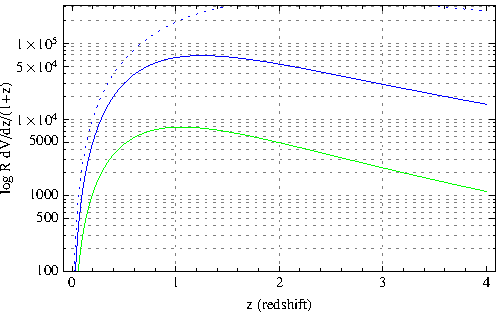
\includegraphics[angle=0,width=0.45\textwidth]{./Sec_ET_ScienceCase/visiondoc-EventRatePerRedshift}
%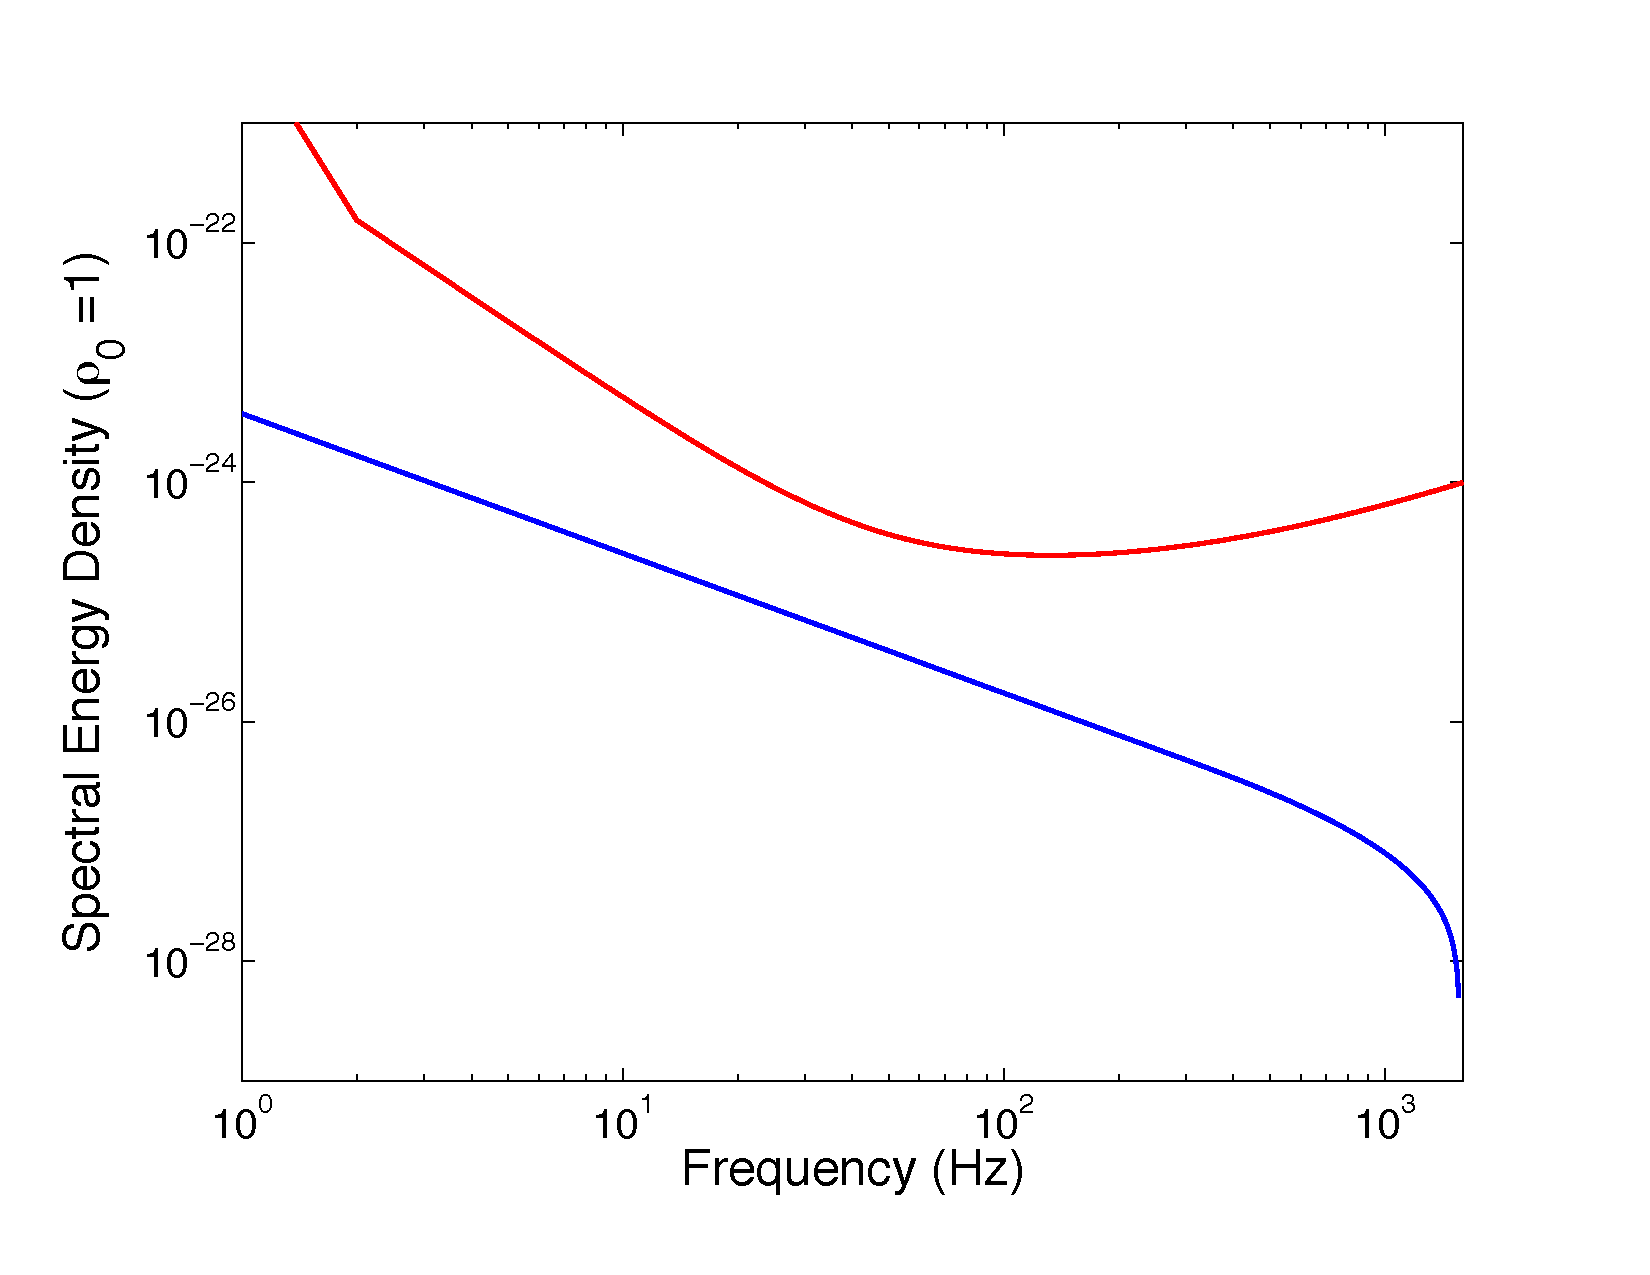
\includegraphics[angle=0,width=0.45\textwidth]{./Sec_ET_ScienceCase/BNS-Sh.pdf}
%\caption{
%Left: The merger rate $dR/dz$  on our past light cone versus  redshift.  Dotted blue 
%line extrapolates  the Milky Way double neutron star merger rate to the universe using
%Eq.~\ref{eq:TrivialMergerEstimate}, which assumes that merger rates trace the star 
%formation history~\cite{sfr-HopkinsBeacom2006} and that the Milky Way forms stars 
%at a rate $dM/dt_{MW}\simeq \dot{\rho}_{MW}/n_{mw} = 3 M_\odot$ yr$^{-1}$.   
%More detailed calculations that account for the finite delay between binary 
%birth and merger are shown in the two sold lines for   NS-NS (blue) and BH-NS (green) 
%binaries.   These delays insure ET will probe the redshift region where most 
%binaries merge.  Right: Spectral energy density of the background produced by 
%the coalescence of double neutron stars, compared to the sensitivity of ET-B.
%\label{fig:DNS_Sh}}
%\end{figure*}

If the stellar binary fraction in a globular cluster is sufficiently high,
two or more IMBHs can form \cite{Fregeau:2006}.  These IMBHs
then sink to the center in a few million years, where they form a binary
and merge via three-body interactions with cluster stars followed
by gravitational radiation reaction \cite{Fregeau:2006,AmaroSeoane:2007aw}. 
Then ET could detect $2000 \left(\frac{g}{0.1}\right) \left(\frac{g_{\rm cl}}{0.1}\right)$ 
mergers per year, where $g$ is the fraction of all globular clusters
hosting pairs of IMBHs, and $g_{\rm cl}$ is the fraction of star forming
clusters.  Mergers between pairs of globular
clusters containing IMBHs can increase this rate by up to a factor of
$\sim 2$ \cite{AmaroSeoaneSantamaria:2009}.
\FloatBarrier
%% \subsubsection{Measurement accuracies}
% \ledby{Van Den Broeck}

\FloatBarrier
\subsubsection{Continuous wave sources}
% \ledby{Krishnan}

Continuous wave sources that are discussed in this section are so-named because
these sources last for at least a few weeks, but typically for months or years, and 
produce signals with roughly constant amplitude and frequency varing relatively 
slowly over the observation time.  Such signals are expected to be
produced by rapidly rotating non-axisymmetric NSs which are
either isolated or in binary systems. A description of the 
signal emitted by such sources is given in Box \ref{box:cw}. There are 
a number of mechanisms which may cause the star to 
emit GWs.  These include deformations of the
NS crust, precession, magnetic fields, and internal oscillation
modes of the NS fluid.  
%([IAN] I dont think more detail is needed in the last sentence, maybe some references though)

%
\paragraph{Isolated neutron stars}

There are at present almost 2000 pulsars known from either radio or
X-ray observations. The parameters of many of these systems, i.e.\  the
sky location and frequency evolution, have been accurately measured. 
In this case we talk of \emph{targeted searches} for known NSs.
We assume the GW phase evolution to be tightly correlated with the
rotational phase as inferred from electromagnetic observations.  For
GW emission due to a non-negligible ellipticity, the
GW emission occurs at twice the rotational frequency of the star.
These two assumptions constrain the expected gravitational waveform
up to an unknown initial phase $\phi_0$, amplitudes $A_{+,\times}$ and
polarization angle $\psi$.  Methods have been developed to search over these
unknown parameters \cite{Jaranowski:1998qm} and to either measure the
amplitude $h_0$, or in the case that no signals are detected, to set
upper limits on it. The main issue in the analysis is how to compensate 
accurately for the Doppler shift due to the source-detector relative 
motion (and other relativistic effects), and the intrinsic spin-down of the source.

The benchmark for these searches is the indirect upper bound on $h_0$ set by
assuming that all of the kinetic energy of the star lost in the
spin-down is channeled into gravitational radiation as illustrated in Appendix 
\ref{box:sdl}. 
This assumption is not expected to hold for any of
the known pulsars where electromagnetic braking explains most of the
spin-down.  Nevertheless, the spin-down limit is still a very useful
benchmark for identifying astrophysically relevant targets and quantifying
search results. Setting an upper limit below the spin-down limit constrains
the fraction of spin-down energy that is emitted as GWs.

Initial interferometers have now set upper limits on a number of known 
pulsars using data from the LIGO, GEO and Virgo detectors
\cite{Abbott:2004ig,Abbott:2007ce, Abbott:2008fx}.  One highlight from
these results is beating the spin-down limit for the Crab pulsar
\cite{Abbott:2008fx} where the GW luminosity is
constrained to be less than $2\%$ of the spin-down luminosity
\cite{Collaboration:2009rfa}. ET will be able to detect continuous waves
from Crab even if it emits one millionth of the spin-down luminosity
in GWs.


\longetbox{i}{box:cw}
{Continuous Gravitational Waves}
{In the case of continuous waves, the waveforms for the two polarizations 
are given by
%
\begin{equation}
  \label{eq:2}
  h_+(t) = A_+\cos\Phi(t), \qquad  h_\times(t) = A_\times\sin\Phi(t),
\end{equation}
%
where $t$ is the time in the frame of the moving, accelerating
detector and $\Phi(t)$ is the phase of the GW; the 
amplitudes $A_{+,\times}$ depend on the other pulsar parameters, 
such as its rotational frequency, moments of inertia, the orientation of 
its rotation axis and its distance from Earth. The phase $\Phi$ takes 
its simplest form when the time coordinate used is $\tau$, the proper 
time in the rest frame of the NS:
%
\begin{equation}
  \label{eq:3}
  \Phi(\tau) = \phi_0 + 2\pi \sum_{n=0}^{s}
  \frac{f_{(n)}}{(n+1)!} \tau^{n+1}.
\end{equation}
%
Here $\phi_0$, $f_{(0)}$ and $f_{(n)}$ ($n\geq 1$)
are respectively the phase, instantaneous frequency and the spin-down
parameters in the rest frame of the star at the fiducial start time
$\tau=0$, $s$ is the number of spin-down parameters included in
the model, and $\iota$ denotes the angle between the line-of-sight to the
star and its rotation axis. It is useful to write the amplitudes
$A_{+,\times}$ in terms of a single number $h_0$
\begin{equation}
  \label{eq:1}
  A_+ = \frac{1}{2}h_0(1+\cos^2\iota) \,,\qquad A_\times = h_0\cos\iota\,.
\end{equation}
The exact expression of the overall amplitude $h_0$ depends on the specific mechanism producing the continuous signal. For instance, in the case of a tri-axial NS rotating with frequency $f_{rot}$ around a principal axis of inertia we have
\begin{equation}
h_0=\frac{4\pi^2G}{c^4}\frac{I_{zz}\epsilon f^2}{d},
\end{equation}
where $I_{zz}$ is the star's moment of inertia with respect to the rotation axis, 
the equatorial ellipticity $\epsilon$ is defined in terms of pricipal axis 
of inertia as $\epsilon=\frac{I_{xx}-I_{yy}}{I_{zz}}$, $d$ is the distance 
to the star and $f=2f_{rot}$ is the signal frequency.
\\[5pt]
The maximum expected signal frequency is below 2\,kHz. Potentially 
interesting sources are within the Galaxy, thus the distance $d\simeq 10$\,kpc. 
The standard value of the moment of inertia is $I= 10^{38}$\,kg\,m$^2$, 
although values in the range $(1-3)\times 10^{38}$\,kg\,m$^2$ are 
considered plausible. The typical values of ellipticity are largely 
unknown; the maximum value allowed by standard equations of state for 
NS matter is $\sim 5\times 10^{-6}$. Some exotic 
equations of state imply maximum values even two orders of magnitude 
larger.
}

The minimum signal amplitude detectable by a given targeted search depends 
directly on the detector sensitivity and scales with the square root of the observation time, as discussed in Appendix \ref{box:h0min}.  

It is informative to compare detectable values of $h_{0,\rm min}$ with the spin-down
limits for a number of known pulsars.
Figure~\ref{fig-CW-known} shows the detectable amplitude for Initial and
Advanced LIGO, Virgo and ET, and the spin-down limits for various known
pulsars. It is clear that the better low-frequency sensitivity of ET-D allows it to
reach the spin-down rate of almost all pulsars with spin frequencies
greater than 3\,Hz (corresponding to a GW frequency of 6\,Hz).
\begin{figure*}
\centering
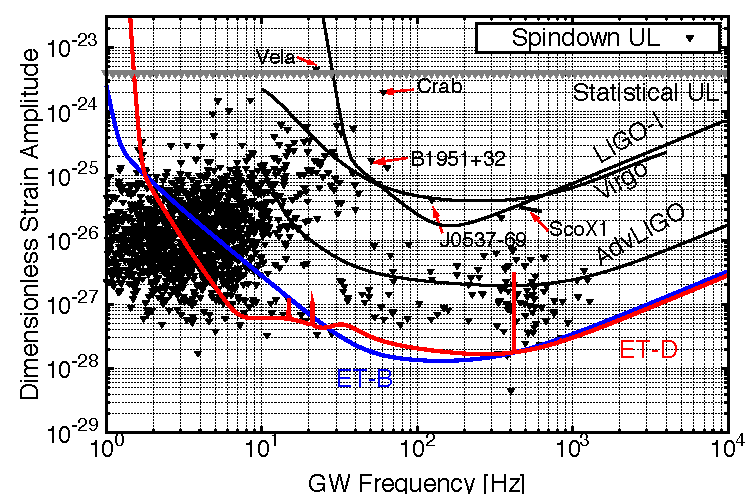
\includegraphics[angle=0,width=0.65\columnwidth]{./Sec_ET_ScienceCase/TheBigPicture_ETBD_5y.pdf}
\vskip 0.3cm
%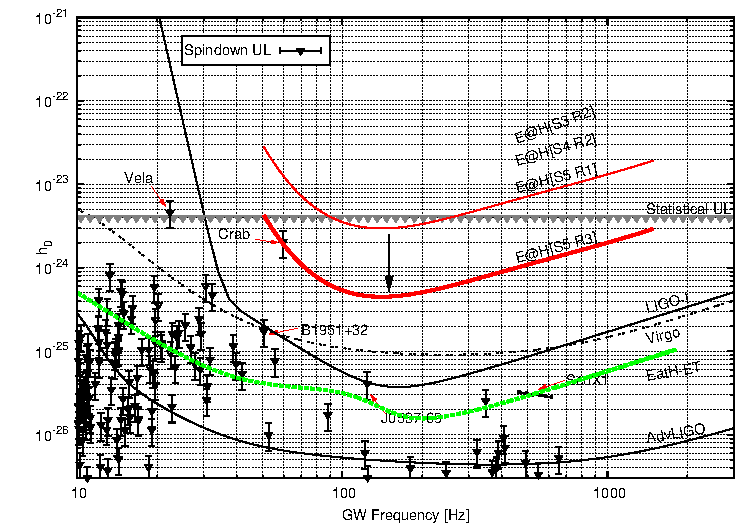
\includegraphics[angle=0,width=0.45\columnwidth]{./Sec_ET_ScienceCase/CW_unknownpulsars}
\caption{
Upper limits and spin-down limits for known pulsars. 
The detector sensitivity curves plot the minimum detectable amplitude 
of the GW averaged over sky positions and pulsar orientations. A detection
threshold based on a false alarm rate of 1\% and a false dismissal rate of 
10\% is assumed.  The spin-down limits assume the NS to have a moment of
inertia in the range 1-3$\times 10^{38}\,\textrm{kg\,m}^2$ and a $\pm
10\%$ uncertainty in its distance.  
% The spindown limit shown in the figure is the average of the upper limits 
% obtained by folding in these uncertainties.  
Initial LIGO and Virgo curves assume an integration time of 2 years while
the rest assume 5 years.  Initial LIGO consists of the H1, L1 and H2
detectors, Virgo is a single detector, aLIGO, ET-B and
ET-D are assumed to consist of three detectors. ET-D's better
sensitivity, compared to ET-B, at frequencies below 20\,Hz 
helps target a number of known pulsars.}
\label{fig-CW-known}
\end{figure*}

Let us turn now to the \emph{wide parameter space searches}. Here, instead of
targeting a known pulsar, the aim is to search for unknown sources in as large 
a portion of the parameter space (sky location, frequency, frequency derivatives) 
as possible.  Potential GW sources could be invisible in the EM band, either
because their radio pulses are not beamed towards us or because their
EM emission is dim due to having a very low magnetic field.
Such searches are computationally limited because the
number of templates increases much faster than linearly with the
observation time $T_{\rm obs}$.  The large number of templates affects the
search sensitivity in three basic ways. The first and most obvious one
is simply the discreteness of the template grid: SNR is lost by searching
for a GW signal with a template that does not exactly match. Secondly, it
leads to a large number of statistical trials, which increases the
false alarm rate and thus leads to a larger 
%effective 
SNR threshold for detection.
Finally, and most importantly, it limits the largest observation time
that can be considered; even given the increase in computer power
following Moore's law, this limitation will most likely still apply in the ET
era.

The problem of computational cost is addressed by the so-called
\emph{semi-coherent} methods. These rely on breaking up the full data
set into shorter segments of duration $T_{\rm coh}$, analyzing the segments coherently and
combining the power from the different segments incoherently. There
are a number of different techniques available for performing the
incoherent combination. %% **cites**.
For these searches, the sensitivity, incorporating all the effects mentioned 
above, is proportional to the square root of the total observation time and 
is given by Eq.~(\ref{hmin_blind}), Appendix \ref{box:h0min}. Typically, the output of a wide-area search 
is a set of \emph{candidates}, i.e.\ points in the source parameter space with 
values of a given statistic above a threshold. These candidates are then 
analyzed in a deeper way \emph{e.g.}\ by making coincidences with another set 
of candidates coming from a different dataset, followed by a full coherent 
analysis on the surviving candidates, in order to confirm or reject them.

%Let us now compare the prospects of detection with two proposed ET 
%sensitivity curves, ET-B and ET-D.
\begin{figure*}
\centering
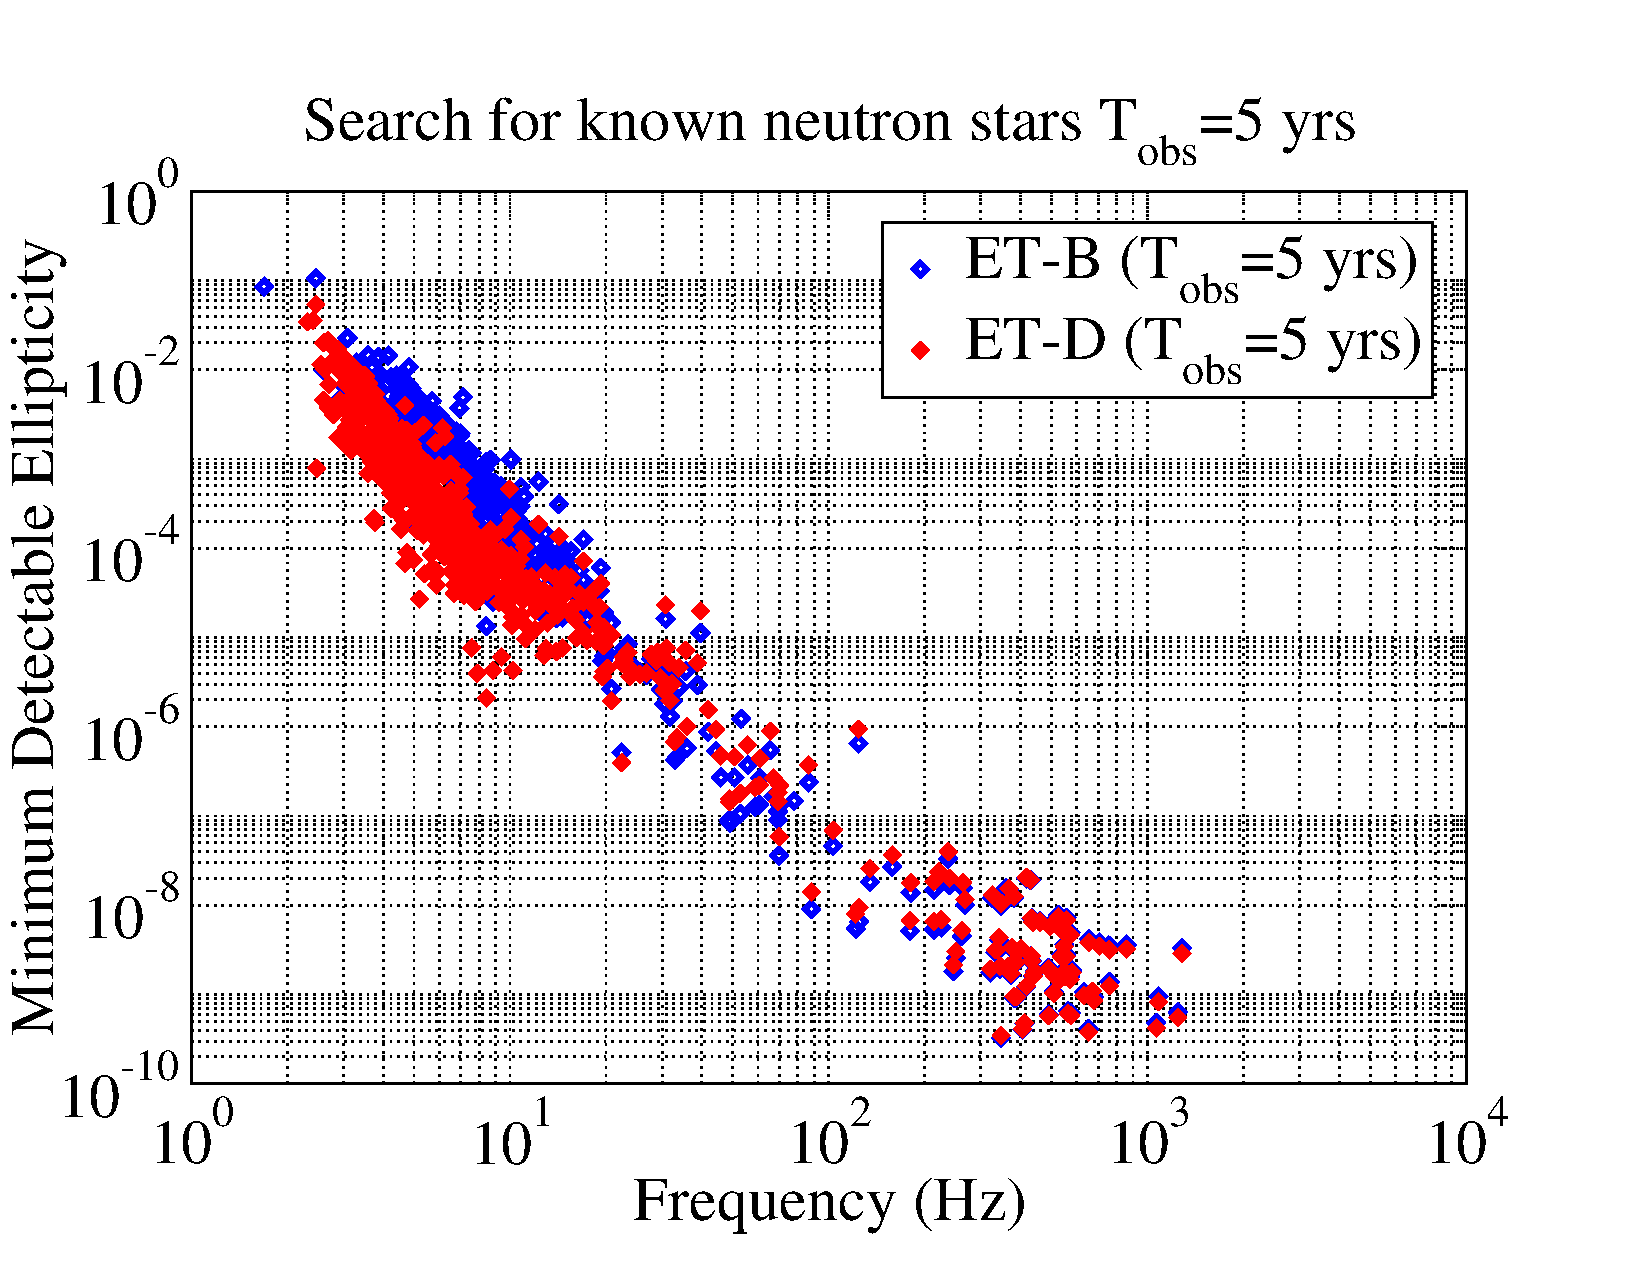
\includegraphics[width=0.49\textwidth]{./Sec_ET_ScienceCase/known_pulsars_ET_epsilon}
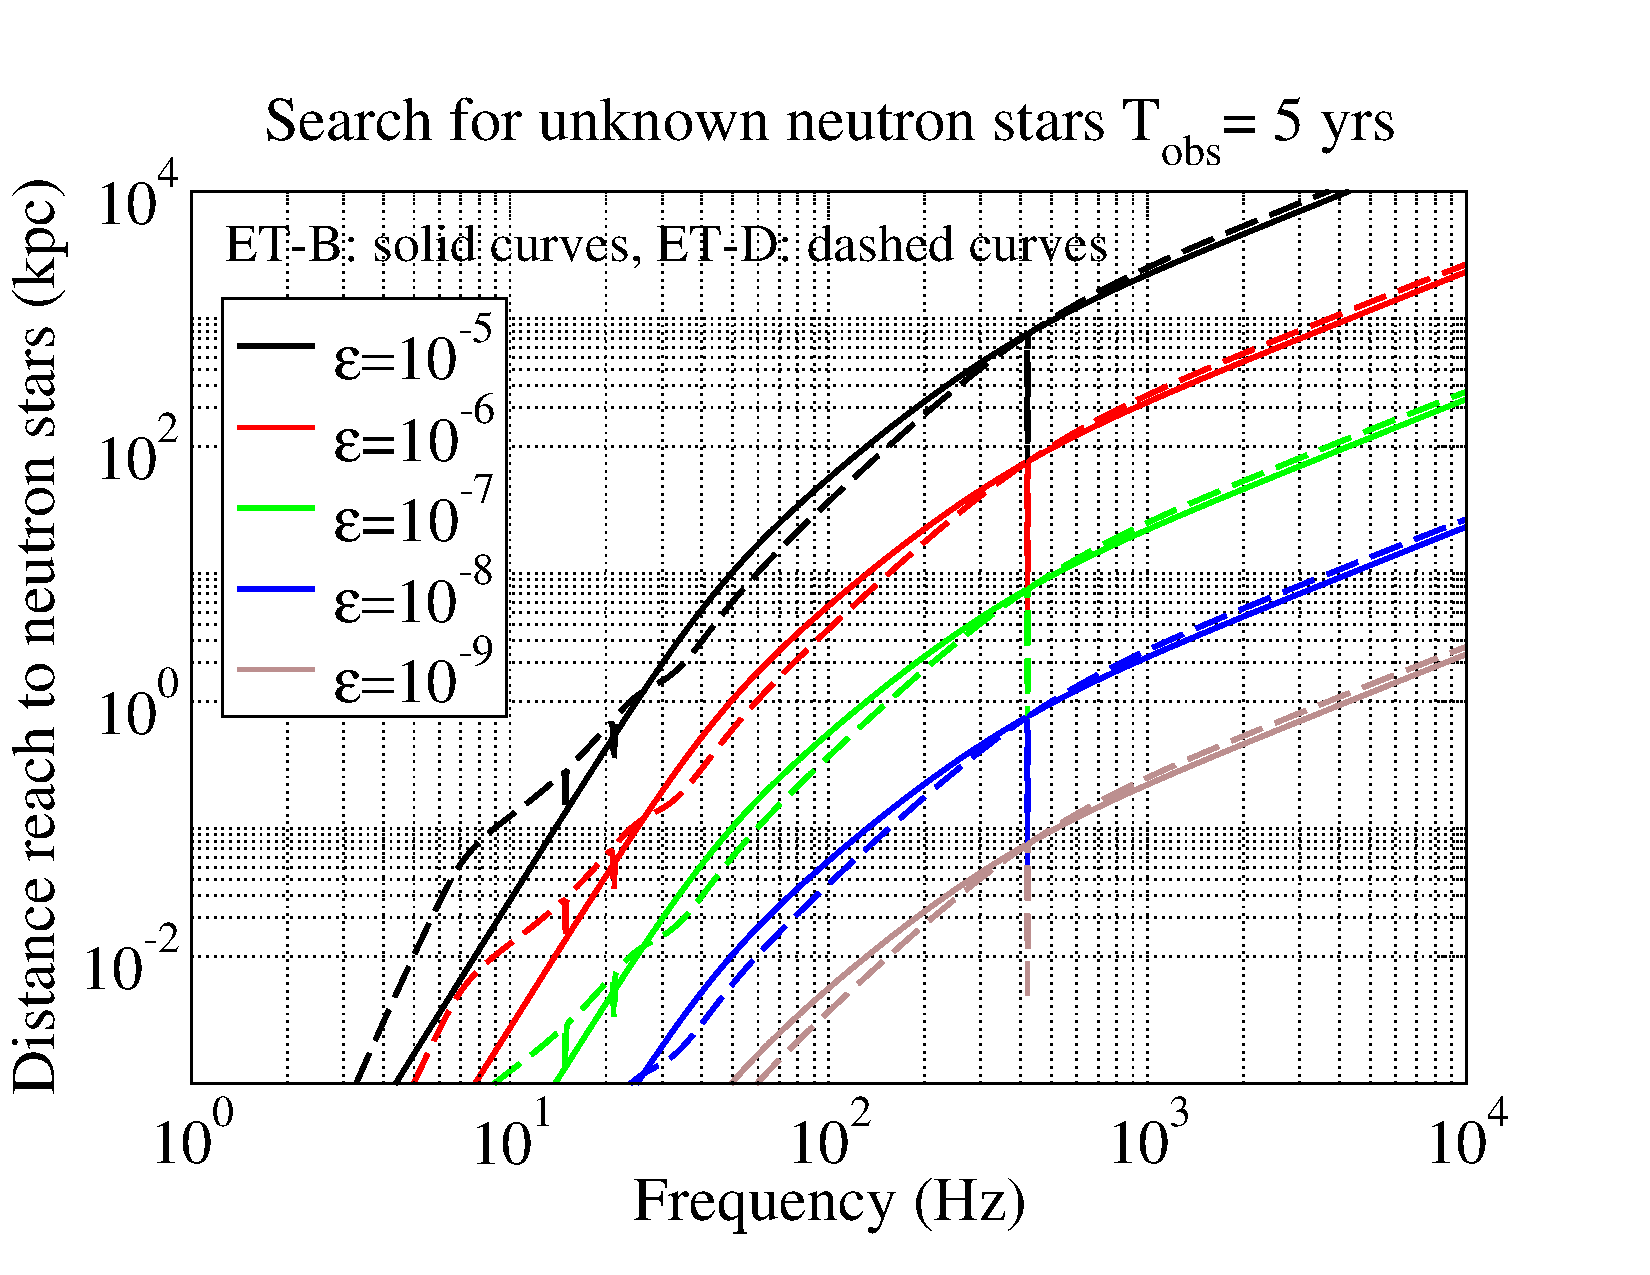
\includegraphics[width=0.49\textwidth]{./Sec_ET_ScienceCase/blind_rmax_ET}
\caption{Left: Minimum detectable ellipticity for known pulsars for 
ET-B and ET-D sensitivities. The search parameters are the same as 
for Fig.~\ref{fig-CW-known}. Right: Maximum distance of an unknown 
source in order to be selected among the candidates of an all-sky 
search with ET-B and ET-D sensitivities. Search parameters are given in the text.}
\label{sensi_knownpulsar}
\end{figure*}
\paragraph{Comparing prospects of detection for ET-B and ET-D sensitivities}
ET-B has a better sensitivity at extremely low frequencies, below $\sim 2$~Hz. 
ET-D, on the other hand, has a better sensitivity in the low frequency range, 
say between $2$\,Hz and $20$\,Hz. At intermediate frequencies, between 
$\sim 30$\,Hz and $\sim 300$\,Hz, ET-B has a slightly better sensitivity. 
The sensitivities of the two configurations are basically the same in the 
high frequency range.  Fig.~\ref{fig-CW-known} plots the minimum detectable
amplitude, assuming ET-B sensitivity (continuous blue line) and ET-D sensitivity 
(dashed red line), with an observation time
$T_{\rm obs}=5\,$yr, a false alarm probability of $1\%$ and a false dismissal
probability of $10\%$ (see Eq.~(\ref{hmin})), versus the spin-down limit of
the known pulsars taken from the ATNF Catalogue at
{\tt http://www.atnf.csiro.au/research/pulsar/psrcat/}. For comparison, the
upper limit reached by Initial and Advanced LIGO and Virgo are also shown but
assuming an integration time of 2 yrs for all except Advanced LIGO, for
which an integration time of 5 yrs is assumed.

We note that no pulsar has yet been found that could emit a
detectable signal with frequency below $\sim 2.5\,$Hz. Thus there
is no gain in having a good sensitivity at extremely low frequencies. On the
other hand, having a better sensitivity around $10\,$Hz impacts positively on
the possibility of detecting a continuous GW signal.

This can be seen also in Fig.~\ref{sensi_knownpulsar}, left panel, where the
ellipticity corresponding to the minimum detectable amplitude is plotted but
only for those pulsars for which the spin-down limit can be beaten in
an observation time of $T_{\rm obs}=5$\,yr. Not only is the number of pulsars for which
the spin-down limit can be beaten far larger for ET-D
but, more importantly, the minimum ellipticity needed to produce a detectable
signal is almost one order of magnitude lower in the $10\,$Hz range.
For instance, with ET-B we typically need $\epsilon$ in the
range $(0.1-5)\times 10^{-4}$ for pulsars emitting around $10\,$Hz, while $\epsilon
\sim (0.1-5)\times 10^{-5}$ is enough with ET-D. There are just a couple of pulsars
at frequencies below $\sim 3\,$Hz for which the spin-down limit could be
beaten with ET-B, but not with ET-D, with corresponding ellipticity in the
$10^{-2}$ range, a value difficult to reach even assuming an exotic equation
of state for NS matter. 

We must, however, keep in mind that the number of pulsars increases with decreasing 
frequency, and so also the probability that
extremely deformed, EM-dim, NSs exist, provided such large
deformations are attainable in nature.
At high frequency, in contrast, there is no relevant difference 
between the two detector configurations and fast spinning pulsars with 
ellipticity less than $\sim5 \times 10^{-8}$ could be detected.

Next, we consider the \emph{blind} search for unknown NSs. In 
this case we plot in Fig.~\ref{sensi_knownpulsar}, right panel, the maximum distance of a 
source to be selected among the candidates of an all-sky, semi-coherent search,
for different values of the NS ellipticity. An
observation time $T_{\rm obs}=5$\,yr and a coherent length 
$T_{\rm coh}=24$\,hr are assumed. Moreover,
the threshold for the selection of candidates is chosen in order to have
$10^9$ candidates.

In practice, we do not expect detections for signal frequencies below
$\sim 10\,$Hz for $\epsilon<10^{-5}$ (the
corresponding $r_{max}$ becomes unrealistically small). And also
considering extremely deformed NSs ($\epsilon> 10^{-5}$)
signal frequencies below $\sim 3\,$Hz are basically excluded. Then, having
a better sensitivity at very low frequencies gives basically no gain. On the
other hand, having a better sensitivity around $10\,$Hz somewhat increases
the possibility of detection: for instance, assuming
$\epsilon=10^{-5}$, the maximum
distance that a search can reach, goes from $\sim 10\,$pc with ET-B to
$\sim 80\,$pc with ET-D at $8\,$Hz, while it goes from $\sim
30\,$pc to $\sim 150\,$pc at $10\,$Hz. On the contrary, in the range 
$\sim 30-100$\,Hz with ET-B the distance reach is about a factor of 2 greater. 

These conclusions do not significantly change assuming a
longer coherent step (compatible with the computing power believed to be
available in the ET era), because the sensitivity increases only as
$T_{\rm coh}^{1/4}$, see Eq.~(\ref{hmin_blind}), Appendix \ref{box:h0min}.

%Observations of accreting neutron stars lead to perhaps the most
%important reason why, irrespective of the mechanism at work, at least
%some neutron stars might be emitting detectable gravitational
%waves.  

%% Spin frequency measurement plays an important role in what follows
%% and, as we shall see, can \cite{Watts2008}

%This is the observation that even the fastest accreting
%neutron stars spin at rates much lower than the expected break-up
%frequency.  The current record is 716\,Hz, %% **cite**,
%while the
%theoretically expected upper limit is more than 1\,kHz. %% **cites**.
%Following a suggestion by Bildsten \cite{Bildsten:1998ey}, it is
%possible that this limit occurs because of the balance between the
%spin-up torque due to the accreting matter, and the spin-down torque
%due to GW emission.  A short calculation assuming a
%link between the observed X-ray luminosity with the accretion rate,
%and taking the mountain scenario for the emission mechanism leads to
%the following estimate of the GW amplitude:
%\begin{equation}
  %\label{eq:6}
  %h_0 = 3 \times 10^{-27}F_{-8}^{1/2}\left(\frac{R}{\rm 10
        %km}\right)^{3/4}\left(\frac{1.4 M_\odot}{M}\right)^{1/4}
  %\left(\frac{{\rm 1~kHz}}{\nu_s}\right)^{1/2}.
%\end{equation}
%This is seen to be depend on frequency: $h_0 \propto \nu_s^{-1/2}$.

\FloatBarrier

\subsubsection{Burst sources}
Many transient astronomical phenomena, such as supernovae, gamma-ray
bursts and glitching pulsars, could produce bursts of gravitational 
waves that last for as short as a few milliseconds (\emph{e.g.}\ supernovae)
to several minutes or longer (\emph{e.g.}\ certain instabilities of NSs, 
discussed below). Detecting such waves, especially in coincidence with optical, 
X-ray, gamma-ray radiation or neutrinos could help resolve decades-old 
problems in astronomy. Gravitational waves will be a very powerful 
addition to multi-messenger astronomy (see~\cite{springerlink:10.1007/s10714-010-1019-z} for a review),  allowing a view into the dark and 
dense cores of sources that are inaccessible to other windows of 
observation.

\paragraph{Gravitational wave bursts from gravitational collapse}
Neutron stars and BHs are formed from the gravitational collapse 
of a highly evolved star or the core collapse of an accreting white
dwarf.  In either case, if the collapse is non-spherical, perhaps induced by
strong rotation or magnetic field, then GWs could 
carry away some of the binding energy and angular momentum, depending 
on the geometry of the collapse. 
Gravitational collapse events are the progenitors of supernovae of 
various types.  Supernovae of Type II are believed to occur at a rate of between 
0.01 and 0.1 per year in a Milky Way equivalent galaxy; thus, within 5\,Mpc,
we might expect an event rate of about 1 per 2 years \cite{ando:05}. 

Simulating gravitational collapse is a very active area of numerical 
astrophysics. Most simulations also predict the energy and spectral 
characteristics of the emitted GWs~\cite{ott:09,Living:Fryer}. 
However, it is still beyond the capabilities of computers to simulate a 
gravitational collapse event with all the physics that might be necessary 
to give reliable predictions: three-dimensional hydrodynamics, neutrino 
transport, realistic nuclear physics, magnetic fields, rotation. In fact, 
it is still by no means clear why Type II supernovae explode at all: simulations 
typically have great difficulty reversing the inflow and producing an explosion
with the observed light-curves and energetics. It may be that the answer lies 
in some of the physics that has to be oversimplified in order to be used in 
current simulations, or in some neutrino physics that we do not yet know.

In a typical supernova, simulations suggest that GWs might extract 
between about $10^{-11}$ and $10^{-7}$ of the total available
mass-energy~\cite{dimmelmeier:08,murphy:09,marek:09b,scheidegger:10b}, and the
waves could come off in a burst whose frequency might lie in the range
of $\sim 200$\,--1000\,Hz.
Using representative values for a supernova in our galaxy, lying at $D=10$\,kpc, 
emitting the energy equivalent of $E=10^{-8}\,M_\odot$ at a frequency of $f=1$\,kHz, 
and lasting for $T=2$\,ms, the observed amplitude would be (cf. \ref{eq:amplitude})
%
\begin{equation}
h \sim 1.5 \times 10^{-21}
\left ( \frac{E}{10^{-7}\,M_\odot} \right )^{1/2}
\left ( \frac{1\mathrm{\,ms}}{T} \right )^{1/2}
\left ( \frac{1\mathrm{\,kHz}}{f} \right )
\left ( \frac{10\mathrm{\,kpc}}{D} \right ).
\label {eq:amplitudeB}
\end{equation}
%
This amplitude is large enough for current ground-based detectors to observe with a
reasonably high confidence, but of course the event rate within 10\,kpc is
expected to be far too small to make an early detection likely. ET can
detect an amplitude that is two orders of magnitude smaller or from a distance
of 1\,Mpc. ET might, therefore, see a supernova collapse once per four or six years.

\begin{figure*}
\begin{center}
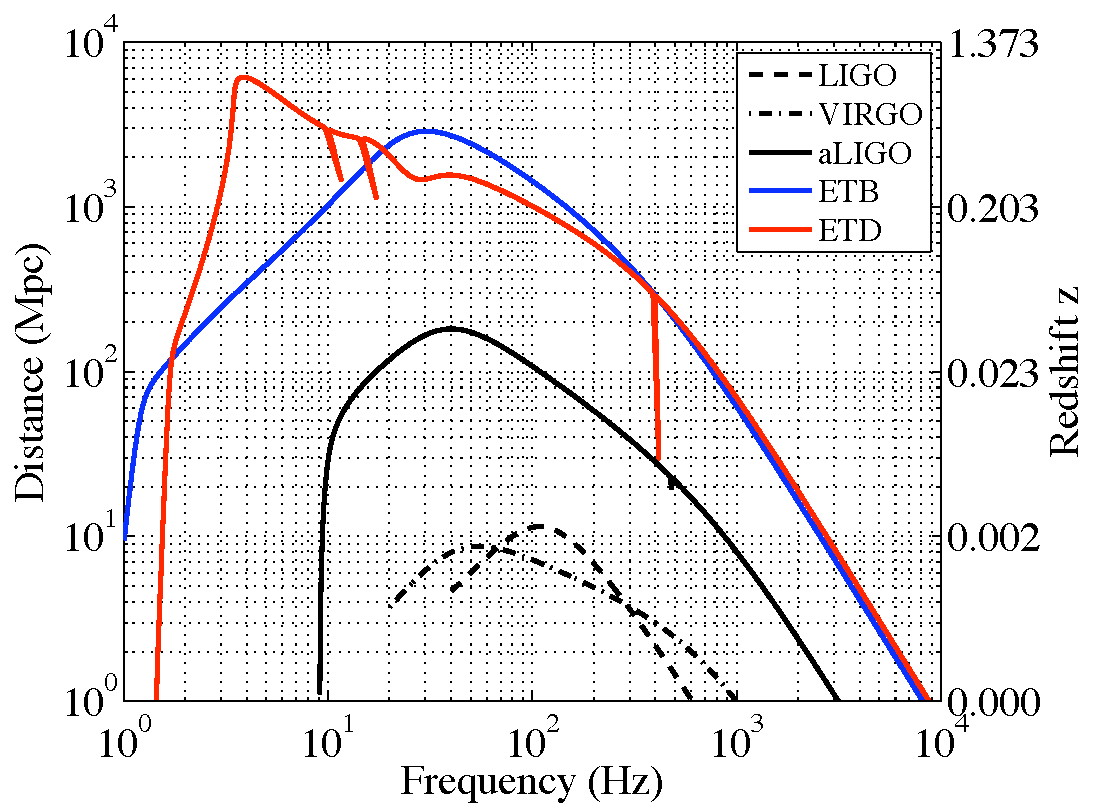
\includegraphics[width=0.60\textwidth]{./Sec_ET_ScienceCase/GWB_distance.pdf}
\caption{90\%-confidence lower limit on distance for GRB burst sources assuming 
a GRB energy emission of $E^{\rm iso}_{\rm GW} = 0.05\,M_{\odot} c^2 \sim 9 \times 10^{52} 
{\rm ergs}$. A redshift correction of $(1+z)$ has been used in computing the lower limit.
\label{fig:distanceFreq_5percentMsol}}
\end{center}
\end{figure*}

\paragraph{Gamma-ray bursts}
There is increasing evidence that gravitational collapse also produces
some of the observed gamma-ray bursts~\cite{Hjorth2003} 
in \emph{hypernovae} and \emph{collapsars}~\cite{Woosley1993, MacFadyenWoosley1999}.
As we shall discuss in more detail, several different classes of GRBs are now known
although their cause is not yet completely understood. There are no
reliable GW emission models from collapsars or hypernovae although some 
estimates give as large as $10^{-2}M_\odot$ for isotropic GW emission for
GRB progenitors.  BNS and NSBH mergers (the likely progenitors of 
most short GRBs) will have isotropic-equivalent emission on the order 
of ($0.01$-$0.1$) $M_\odot$ in the 100 to 200 Hz band. For long GRBs, 
fragmentation of the accretion disk \cite{davies:2002,king:2005,piro:07}
could produce inspiral-like chirps with $(0.001$-$0.01)\,M_\odot$ emission 
in GW.  The suspended accretion model \cite{vanPutten:grb} also
predicts an energy emission of up to $(0.01$-$0.1) M_\odot$ in this
band.


A GRB at a distance of $D=4.2\,\rm Gpc$ (a redshift of $z\simeq 0.7$) 
emitting the energy equivalent of $E=5\times 10^{-2}\,M_\odot$ 
at a frequency of $f=1$\,kHz, and lasting for $T=1$\,ms, produces an amplitude of~\cite{springerlink:10.1007/s10714-010-1019-z}
%
\begin{equation}
h \sim 10^{-23}
\left ( \frac{E}{5\times 10^{-2}\,M_\odot} \right )^{1/2}
\left ( \frac{1\mathrm{\,ms}}{T} \right )^{1/2}
\left ( \frac{1\mathrm{\,kHz}}{f} \right )
\left ( \frac{4.2 \mathrm{\,Gpc}}{D} \right ),
\label {eq:amplitudeC}
\end{equation}
%
Figure \ref{fig:distanceFreq_5percentMsol} shows the distance 
reach of Initial and Advanced LIGO, Virgo and two possible noise curves considered
for ET (ET-B and ET-D)
to such a GRB. The waveform emitted in the process is not known with any certainty
and so the distance reach is calculated by assuming that GW bursts are detected
by search algorithms that look for excess energy in a time-frequency map.
While aLIGO might detect rare closeby GRBs, ET could probe GRBs at cosmological
distances, assuming GWs extract about $0.05\, M_\odot$ in the process.


\paragraph{Pulsar glitches and magnetar flares}
Neutron stars have a rich spectrum of non-radial normal modes, which 
which can be classified according to key key restoring force that 
affects the fluid motion. In the context of GW astrophysics f-, g-, p-, w-, 
and r-modes have all been studied~\cite{AnderssonKokkotas1998,Andersson:2003}.  
Just as in the case of BHs, these normal modes are a superposition of 
damped sinusoids, but in the NS case the frequencies and damping times 
depend on the complex physics of NS interiors.  Modelling the NS oscillation 
spectrum requires physics beyond what is within reach for laboratory 
experiments. This sets a severe challenge, but at the same time it is a key 
reason why the problem is important. It also provides ample motivation for 
attempts to provide observations that can be used to test various theoretical 
models, e.g. concerning the state of matter at extreme densities. A promising, 
at least in principle, strategy follows the very successful asteroseismology 
programme for normal stars. In the case of the sun, the matching of inferred 
non-radial oscillation modes to theoretical predictions has led to a much 
improved understanding of the interior conditions. Similarly, one may expect 
that GW observations of oscillating NSs may place useful constraints both 
on bulk parameters like mass and radius, and hence the overall EoS, and 
detailed physics, like internal composition gradients.  In fact, even 
knowing accurately the frequency and decay time of just the fundamental 
$\ell=2$ f-mode would be enough to eliminate most currently considered 
equations of state~\cite{AnderssonKokkotas1998}.

The f-modes of NSs are promising emitters of GWs that may be excited 
by glitches or by the nuclear explosions on accreting neutron stars that 
are thought to produce X-ray flares and soft gamma-ray repeater events. 
The rise-time of X-ray emission can be as short as a few 
milliseconds\,\cite{2008Kes75}, which might be impulsive enough to excite 
acoustic vibrations. If the rise time of the explosion matches the period 
of the mode well enough, then a substantial fraction 
of the energy released could go into mechanical vibrations, and almost all of this 
fraction would be carried away by GWs, since other mode-damping mechanisms 
inside NSs tend to be less efficient. 

The viability of these scenarios is difficult to quantify, given our general 
lack of understanding of the detailed dynamics associated with them. 
Presently, most available models are based on back-of-the-envelope 
phenomenology. This is well illustrated by the radio-pulsar glitches, 
enigmatic spin-up events seen in (mainly) relatively young NSs like Crab and Vela. 
It is easy to estimate that these events are associated with energies of 
order $ 10^{42}$~erg ($10^{-12}\,M_\odot$). This sets a useful benchmark 
energy level for discussion of GW events associated with NS in our galaxy, 
but it obviously does not constitute a real estimate of the energy 
released as GWs.  Nevertheless, assuming this level of energy emission 
through the f-mode at 2~kHz of a star at a distance of 10~kpc it is easy 
to estimate that these events could create a wave of effective amplitude 
(see Eq.\,\ref{eq:amplitudeB}) around $10^{-23}$. (The effective amplitude 
assumes we can do matched filtering, which in this case is not very 
difficult.) This kind of amplitude should be well within the reach of ET.  
Observations of these modes would immediately constrain the cold-matter 
nuclear EoS in significant ways~\cite{AnderssonKokkotas1998, Living:AnderssonComer}.

It is also important to note that NS events seen in X-rays and gamma rays 
can be much more energetic.  In fact, NS oscillations may have already been 
observed in X-rays~\cite{WattsStrohmayer2007}. Quasiperiodic oscillations 
seen in the tails of strongly magnetised NS (magnetar) flares agree well 
with predicted crustal modes, whose restoring force is the shear strength 
of the crust. These observations mainly probe  the physics of the crust, 
which represents the low-density region and is not expected to leave a 
strong imprint on emitted GWs. Nevertheless, the observations 
allows us to test the astero-seismology paradigm \cite{Samuelsson:2007}, 
an exercise that has placed (weak) constraints on the EoS. As far as GW 
astrophysics is concerned, a key question concerns to what extent the 
more massive NS core takes part in these event. The general expectation 
is that the magnetic field provides an efficient coupling 
between the crust and the core. The upshot of this could be that the 
magnetar events are predominantly due to the interior magnetic dynamics, 
which may make them associated with detectable GWs. Establishing this 
requires better theory modelling, but it is still clear that ET will 
be able to place useful constraints on any such mechanism.


\paragraph{Relativistic instabilities of compact stars} The most 
promising scenarios for detectable NS oscillations involve some 
kind of instability. Realistic NS may become unstable during 
different evolutionary stages. A rapidly and differentially rotating 
proto-NS may be dynamically unstable due to the so-called bar-mode 
(the l=m=2 f-mode). At less extreme differential rotation, the 
so-called low T/W instability may operate. Proto-NSs may also be 
convectively unstable, leading to growing g-modes, due to temperature 
gradients. The mechanisms connect the birth of a NS with the 
supernova event, and the level of excitation of the involved 
oscillations depends to a large extent on how the core-collapse 
proceeds. Another class of instabilities is powered by with the 
emission of GWs. First demonstrated by Chandrasekhar~\cite{ChandraCFS} 
in 1971, this instability was shown to be generic in rotating stars 
by  Friedman and Schutz~\cite{Friedman1978}  a few years later. They 
proved that the unstable modes have a very simple signature depending 
on the pattern speed of the mode, i.e.\ the angular velocity at which 
the crests of the pattern passes about the rotation axis of the star. 
If this velocity is in the same sense as the rotation of the star, 
but slower than that of rotation, then the mode would be unstable in 
a perfect fluid star. This instability has come to be known as the 
CFS instability, after the three authors who discovered and explained 
it.  

The presence of an instability is, however, not sufficient to make 
the scenario astrophysically relevant. In order to play a role for 
real NSs, any instability must overcome a number of damping mechanisms. 
The problem then becomes exceedingly difficult, especially since we 
do not have very precise models for the various transport coefficients 
needed for a model of NS dissipation. Nevertheless, there has been 
considerable progress on this problem. Focussing on the instability 
associated with the f-mode, Lindblom and Detweiler~\cite{LINDBLOM1977} 
showed that the effect of viscosity runs counter to that of radiation 
reaction, so that the instability is strongest in modes with the 
longest wavelengths,  in principle the quadrupole modes. However, 
numerical calculations for Newtonian stellar models with realistic 
viscosity show~\cite{Lindblom:1995zs} that the f-modes are not vulnerable 
to the instability. This would weakens the impact for GW physics 
significantly. In addition to this, it has been demonstrated that the 
friction associated with superfluid vortices may suppress the 
instability entirely \cite{Lindblom:1995zs}.
These results do not, however, signal the demise of this mechanism. 
First of all, the instability is stronger in fully relativistic 
models~\cite{Stergioulas:1997ja}, especially since the $l=2$ mode 
may also be unstable.  Secondly, the superfluid friction becomes 
relevant only after the star has cooled below the relevant transition 
temperature (below $10^9$~K). Hence, there may still be room for the 
f-mode instability to play a relevant role in very young NSs. Moreover, 
as the f-mode is an ideal GW emitter (with a short instability growth 
time, and possible large nonlinear amplitude) the associated signals 
may well be within reach with ET even for extragalactic sources. This 
is an interesting possibility that need to be explored by more detailed 
modelling. 

Most recent activity on NS instabilities has concerned a different 
class of oscillations, namely the Rossby, or r-modes. In contrast 
to the f-modes, which become unstable above a critical rotation rate, 
these modes are unstable in a rotating perfect fluid star at all 
rotation rates. The associated GWs comes from the current-multipoles, 
rather than from the mass multipoles as in the case of the f-mode. 
This makes the modelling different, but the main physics issues 
remain the same. Investigations by a number of authors~\cite{Lindblom:1998wf, 
Andersson1999, Owen1999} have shown that the r-mode instability could 
be relevant in hot, rapidly-rotating stars.  In particular, it may 
lead to a nascent NS spinning down significantly, losing angular 
momentum as GWs.  The instability might also operate in mature, 
accreting NSs, such as those in low mass X-ray binaries (LMXB) 
(see the next section). 

In principle, the fact that the r-mode instability window depends on 
a balance between GW driving and various dissipation mechanisms makes 
it a sensitive probe of NS core physics.  Observations allow us to 
test our understanding of exotic physics associated with 
hyperons~\cite{LindblomOwen2002, Lackey2006}. , deconfined quarks and 
large scale superfluids/superconductors \cite{Living:AnderssonComer}. 
The signal associated with various r-mode scenarios should be 
detectable with ET for systems within, and possibly beyond, our 
galaxy \cite{Bondarescu:2009}
but in order to facilitate such detections we need to make progress 
on thorny theory issues. Key issues concern the interaction with 
magnetic fields in the star, the damping due to the vortex mediated 
mutual friction in a superfluid , the possible role of turbulence, 
the boundary layer at the crust-core interface and exotic bulk viscosity 
due to the presence of hyperons or deconfined quarks in the deep 
neutron star core. These problems are all very challenging. In addition, 
we need to  model the GW signal from an unstable r-mode. This is also 
difficult because, even though the r-mode growth phase is adequately 
described by linear theory, nonlinear effects soon become important 
leading to the evolution, and the  associated GW signal, becoming 
very complex.  Future ET observations have the potential to test 
various proposed r-mode scenarios, improving our understanding of 
extreme NS physics significantly.   


\FloatBarrier
\subsubsection{Stochastic background} \label{source_stochastic}
The superposition of a large number of unresolved sources of GWs 
produces a stochastic background.  We can distinguish between two 
contributions: a primordial background of cosmological origin, a 
memory of the early stages of the Universe, and a background of 
astrophysical origin, a memory of the evolution of the galaxies 
and star formation. We summarize basic properties of a stochastic 
GW background in Box~\ref{box:stoch_basics}. The strength of the
background is characterized by the dimensionless quantity
$\Omega_{\rm GW}(f),$ which is the ratio of the energy density
in GWs to the critical density of the Universe as a function
of frequency. 

\paragraph{Primordial background}
The essential interest of a primordial GW background is the prospect 
of probing the behaviour of matter and the evolution of the Universe 
at very high energy scales and densities---potentially even above the 
energies achievable at current particle colliders. This is feasible 
thanks to the very large redshift factor (well over ten orders of 
magnitude) appropriate to times before primordial nucleosynthesis: 
waves created at extremely short length scales may now be accessible 
to terrestrial detectors. At such short distance scales and high 
energies, evidence for new physics may emerge, such as particles 
beyond the Standard Model, high-temperature phase transitions and 
topological defects, inflation and reheating, or even extra spatial 
dimensions.  

\etbox{i}{box:stoch_basics}{The Spectrum of Stochastic GW Background}
{
It is usual to characterize the intensity of a random field of 
GWs by its energy density as a function of 
frequency.   Since the energy density of a plane wave is the same 
as its flux (when $c=1$), we have from Eq.\,(\ref{eq:flux})
$\rho_{\text{GW}} = \pi f^2h^2/4.$
But the wave field in this case is a random variable, so we must replace $h^2$ 
by a statistical mean square amplitude per unit frequency 
(Fourier transform power per unit frequency) called $S_{\mathrm{GW}}(f)$, 
so that the energy density \emph{per unit frequency} 
is proportional to $f^2 S_{\mathrm{GW}}(f)$.  It is then conventional to talk about the 
energy density per unit logarithm of the frequency, which means multiplying by $f$.    
The result, after being careful about averaging over all directions of the 
waves and all independent polarization components, is~\cite{Allen:1997ad, Thorne1987}
\begin{equation}
\frac{{\rm d}\rho_{\text{GW}}}{{\rm d}\ln f} = 4\pi^2 f^3 S_{\mathrm{GW}}(f).
\end{equation}
What is of most interest is the energy density as a fraction of the 
closure or critical cosmological density, given by the Hubble constant 
$H_0$ as $\rho_c = 3H_0^2/8\pi$.  The resulting ratio is called $\Omega_{\text{GW}}(f)$:
\begin{equation}
\Omega_{\text{GW}}(f) = \frac{10\pi^2}{3H_0^2}f^3S_{\mathrm{GW}}(f).
\label{eq:stochastic}
\end{equation}
%\\[5pt]
%For a stochastic background of astrophysical origin:
%\begin{equation}
%\Omega_{\rm gw}(\nu_o)=5.7 \times 10^{-56}  \nu_o \int_{z_{\min}}^{z_{\max}} \frac{\dot{\rho}^o(z)}{(1+z)E(z)}\frac{dE_{\rm gw}}{d\nu}(\nu_o)dz
%\end{equation}
%where $\dot{\rho}^o(z)$ is the number of events in an element of comoving volume and interval of time in the observer frame, $\frac{dE_{\rm gw}}{d\nu}$ the typical spectral energy density of a single source and $E(z)$ a function that depends on the cosmology. 
%\\[5pt]
To evaluate the contributions of various sources to the background we 
take a fiducial value $H_0=70$\,km\,s$^{-1}$\,Mpc$^{-1}$ for the Hubble 
parameter and assume a flat Universe with $\Omega_\Lambda = 0.7$.
}

\begin{figure*}
\centering
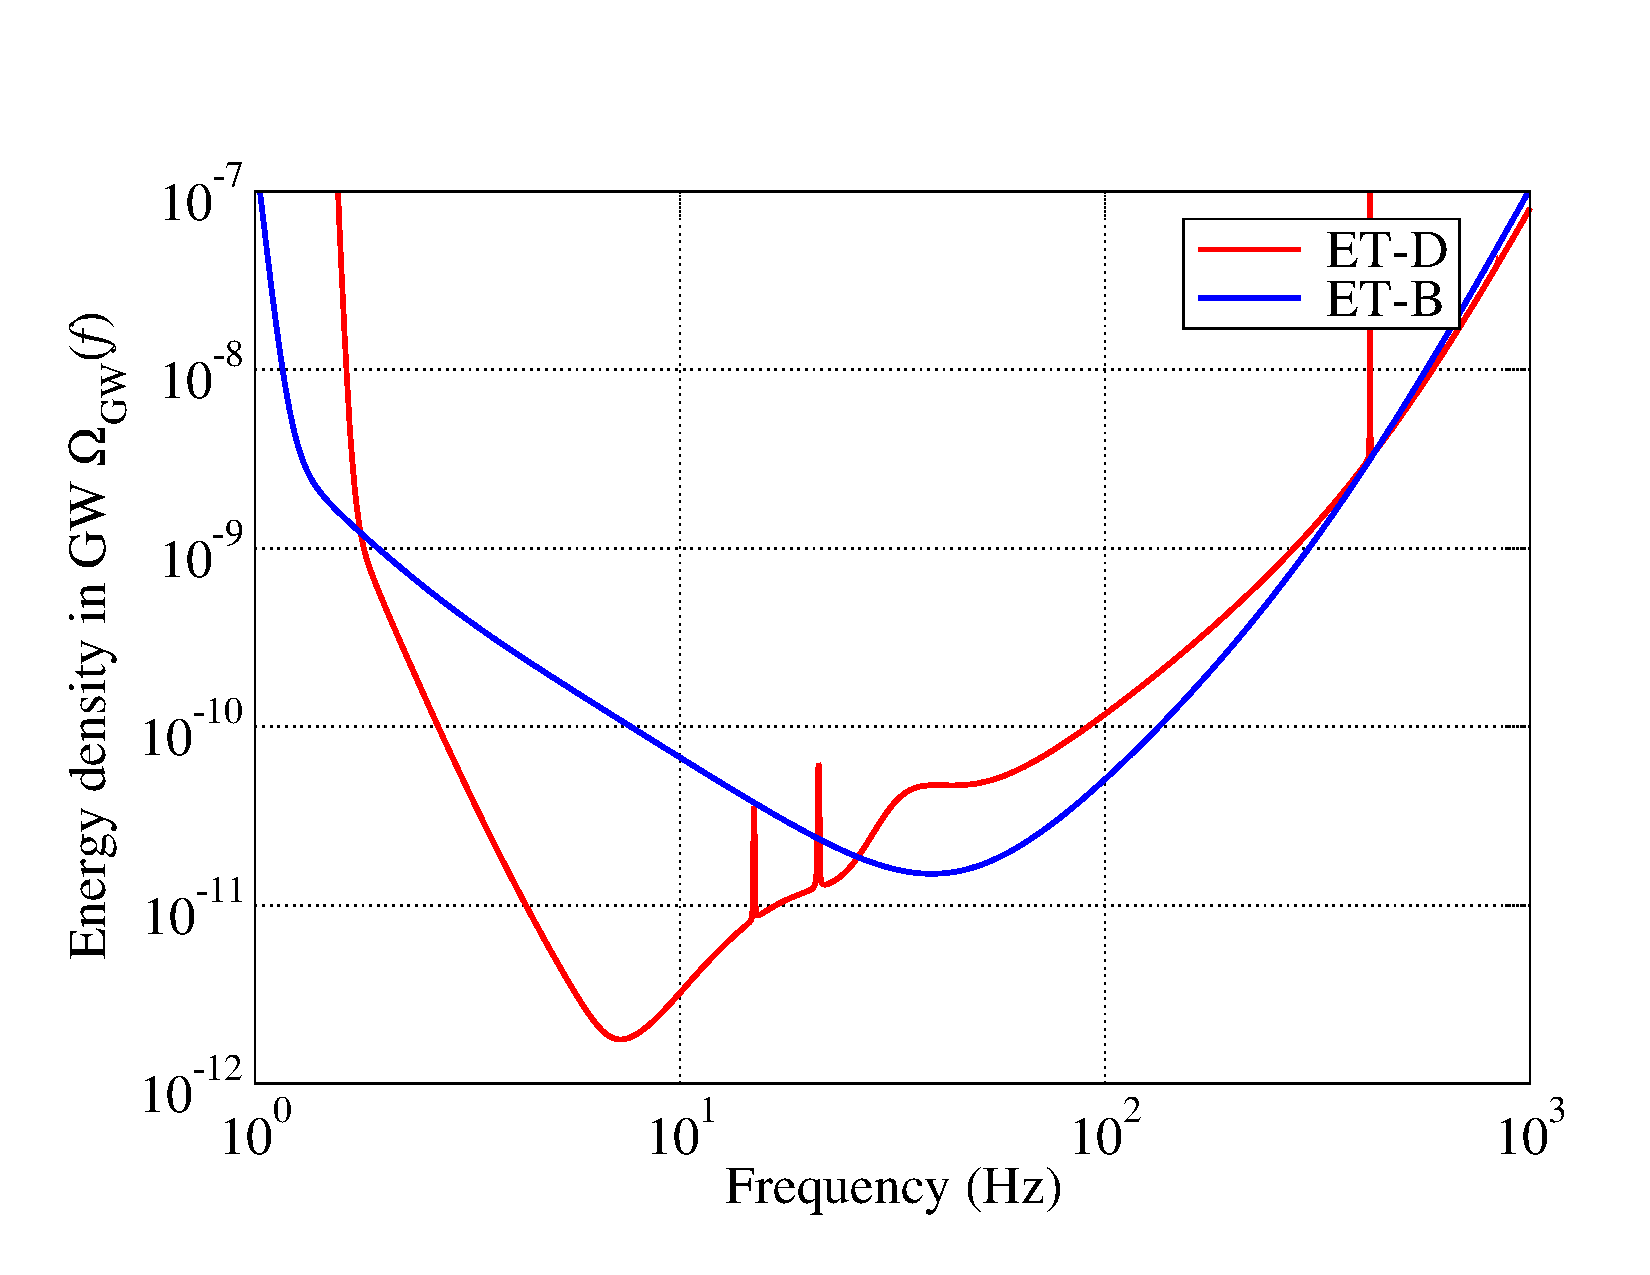
\includegraphics[width=0.60\textwidth]{./Sec_ET_ScienceCase/GWB.pdf}
\caption{The sensitivity ET-B and ET-D detectors to
stochastic background of GW. The curves show the energy density in GW that 
ET would be sensitive to after a year's integration at 95\% 
confidence level.}
\label{fig:stochastic}
\end{figure*}

The ultimate goal of detector development is the observation
of the background radiation from the Big Bang. It is expected to be very weak, 
but it will come to us unhindered from as early as $10^{-30}$~s, and it could 
illuminate the nature of the laws of physics at energies far higher than we 
can hope to reach in the laboratory. 

\paragraph{Astrophysical background}
The astrophysical contribution is important for at least two reasons.
On the one hand, it may mask the cosmological background in some 
frequency windows;  on the other hand, its detection would put 
strong constraints on the physical properties of compact objects 
and their evolution with redshift, such as the mass of NSs or BHs, the 
ellipticity and the magnetic field of NSs or the rate of 
compact binaries.

What is particularly interesting is that using stochastic backgrounds, 
we are able to put constraints on the mean values and not on the 
properties of the brightest sources, more likely in the tail of the 
distributions. 



\paragraph{Detecting stochastic backgrounds}
Random radiation is indistinguishable from instrumental noise in a single 
detector, at least for short observing times. If the random field is produced by
an anisotropically-distributed set of astrophysical sources (the binaries in our 
galaxy, for example) then over a year, as the detector changes its orientation, the 
noise from this background should rise and fall in a systematic way, allowing 
it to be identified. But this is a rather crude way of detecting the radiation, and 
a better way is to perform a cross-correlation between two detectors, if available. 

In cross-correlation, which amounts to multiplying the outputs and integrating, the 
random signal in one detector essentially acts as a template for the signal in the 
other detector. If they match, then there will be a stronger-than-expected correlation. 
Notice that they can only match well if the wavelength of the GWs is longer
than the separation between the detectors: otherwise time delays for waves reaching one 
detector before the other degrade the match. In this regard, ET's topology is 
particularly important. Since it hosts several detectors at the same location there
is no time delay involved and hence all frequencies contribute to the cross correlation.

The outcome of cross-correlation is not like standard 
matched filtering, however, since the ``filter'' of the first detector has as much 
noise superimposed on its template as the other detector. As a result, the 
amplitude SNR of the correlated field grows only with observing time as $T^{1/4}$, 
rather than the square root growth that characterizes matched filtering~\cite{Thorne1987};
sensitivity to $\Omega_{\rm GW},$ however, grows as $\sqrt{T}.$ 
\paragraph{ET's sensitivity to stochastic background}
The only tight constraint on  
$\Omega_{\text{GW}}$ from non-gravitational-wave astronomy is that it 
must be smaller than $10^{-5}$, in order not to disturb the agreement 
between the standard Big Bang model of nucleosynthesis (of helium and
other light elements) and observation. If the Universe contains
this much gravitational radiation today, then at the time of
nucleosynthesis the (blue-shifted) energy density of this radiation
would have been comparable to that of the photons and the three
neutrino species. Although the radiation would not have participated
in the nuclear reactions, its extra energy density would have required
that the expansion rate of the Universe at that time be
significantly faster, in order to evolve into the Universe we see
today. In turn, this faster expansion would have provided less time
for the nuclear reactions to ``freeze out'', altering the abundances
from the values that are observed today~\cite{Pagel:2000,Steigman:2007xt}. 

First-generation interferometers have already set direct limits 
\cite{Abbott:2009ws} on the cosmological background below the 
nucleosynthesis limit at $\Omega_{\rm GW} < 6.9\times 10^{-6}.$ 
Figure \ref{fig:stochastic} plots the sensitivity of Advanced LIGO
and ET to stochastic backgrounds assuming cross-correlation of data
over a period of one year. The plot is constructed using the formula 
(\ref{eq:stochastic}) taking $S_{\rm GW}=2.56\,S_h(f)/\sqrt{f\,T_{\rm yr}},$
where $S_h(f)$ is the noise power spectral density of the detector
in question, $T_{\rm yr}$ is the number of seconds in a year and a
factor of 2.56 is inserted to account for the SNR needed for a 95\%
confidence level.  Advanced detectors will probe stochastic backgrounds of strengths
$\Omega_{\rm GW} \sim 10^{-9}$ (see Fig.~\ref{fig:stochastic}) but
ET, thanks to its better low-frequency sensitivity, could detect
backgrounds at levels approaching $\Omega_{\rm GW} \sim 10^{-12}$ 
around frequencies of 10\,Hz. 

Sections \ref{cosmo_stochastic} and \ref{astro_stochastic}
discuss possible sources of stochastic backgrounds of primordial
and astrophysical origin and the physics we can
learn by detecting such backgrounds with ET.

\clearpage

\FloatBarrier
\subsection{Fundamental physics and strong field tests of GR}

The rich variety of sources and phenomena observed by
GW detectors can potentially be used
to address outstanding questions in fundamental physics.
The sources in question will be in dense environs
of ultra-strong gravity and will therefore provide a cosmic
laboratory for understanding phenomena and matter in
extreme conditions of density, temperature, and/or magnetic
fields. Moreover, BBH are
fundamentally geometric objects whose interaction close
to merger will provide insights into the nature of 
BH spacetimes and of gravity in ultra-strong fields.
Here we will discuss what fundamental physics
questions and strong-field tests of gravity could be
addressed by ET.

\FloatBarrier
\subsubsection{Polarization of gravitational waves}
In Einstein's theory of gravity, GWs have only two polarizations, 
the plus and cross polarizations discussed in Box \ref{box:gw}. 
In scalar-tensor theories GWs have four polarizations more 
than in GR. Observations of gravitational waves 
could exploit this difference to test GR.

In the long
wavelength approximation (i.e.\ when the wavelength is
much longer than the typical distance between test masses),
plus and cross polarizations cause quadrupolar deformations
in space and the proper distance between test masses changes
in a direction transverse to the propagation of the waves 
(see Fig.\,\ref{fig:pol}, Box \ref{box:gw}).  Other 
polarizations could cause motion of test masses longitudinal
to the direction of propagation as well as other patterns 
in the transverse plane. 

ET, with its three interferometers, will be able to resolve
the two polarizations, assuming that GR is the correct description
of gravity. With a network of other advanced or third generation
detectors that might be available at the time one could independently 
measure the polarization and check if the two measurements are
consistent with one another. Conclusively showing (to within 
experimental uncertainties) the absence of other polarizations 
could rule out a whole class of alternatives to GR. Advanced
detectors could do this to some extent but high SNR events that
ET is likely to see will provide compelling evidence.


\subsubsection{Bounding graviton mass}
% \ledby{Arun: June 8th}\\
In Einstein's theory, gravitational radiation travels at
the speed of light.  This means that gravitons, the particle
counterparts of GWs, are massless particles.
Although there is currently no strong motivation to
consider massive graviton theories from an experimental
point of view, they are natural extensions of Einstein's
theory.  In a massive graviton theory, GWs
would not travel at the speed of light and this can be
tested by observation of gravitational-wave sources
at very great distances.  To do so we would need a
source which emits both GW and EM radiation simultaneously.
By measuring the difference in their arrival times we could 
measure or constrain the speed of GWs.

Supernovae and BNS and NSBH systems are sources that are expected to 
exhibit after-glows in EM radiation soon after they emit a burst of GWs. 
If the source is near enough (a few Mpc in the case of supernovae, and
redshifts of a few in the case of coalescing binaries) and the
event is well-localized on the sky (fraction of a
degree depending on the distance to the source),
then it could be observed in coincidence as a transient
EM and GW event.

Current theories of supernovae and coalescing binaries
cannot accurately predict how promptly after the collapse
(in the case of SN) or merger (in the case of binaries)
EM radiation will follow. However, the expected delay is
no more than one second.
If GWs arrive a time $\Delta t$ after EM
waves, then the fractional difference in their speeds is
given by
\begin{equation}
\frac{|\Delta v|}{c} = 3.2 \times 10^{-18}
\left ( \frac{|\Delta t|}{1\,\rm s} \right )
\left ( \frac{3\, \rm Gpc} {D} \right )
\end{equation}
where we have assumed that the source is at a distance of
$D=3\,\rm Gpc$. This can be used to constrain the graviton
mass but there is a more robust method that could yield
better upper limits.

Gravitational waves in a massive graviton theory would suffer disperson and
the effect would be greater the farther an observer is from the source.
Thus, observations of inspiralling compact binaries at high redshifts
can be used to place better bounds on the mass of the graviton, or equivalently
the Compton wavelength of the graviton~\cite{bss:will.98}, than is possible
by comparing the arrival times of GW and EM radiation from a source. Moreover, 
bounds from GW dispersion do \emph{not} require the detection of an EM counterpart 
associated with the GW signal.
%
\begin{figure}[t]
\centering
%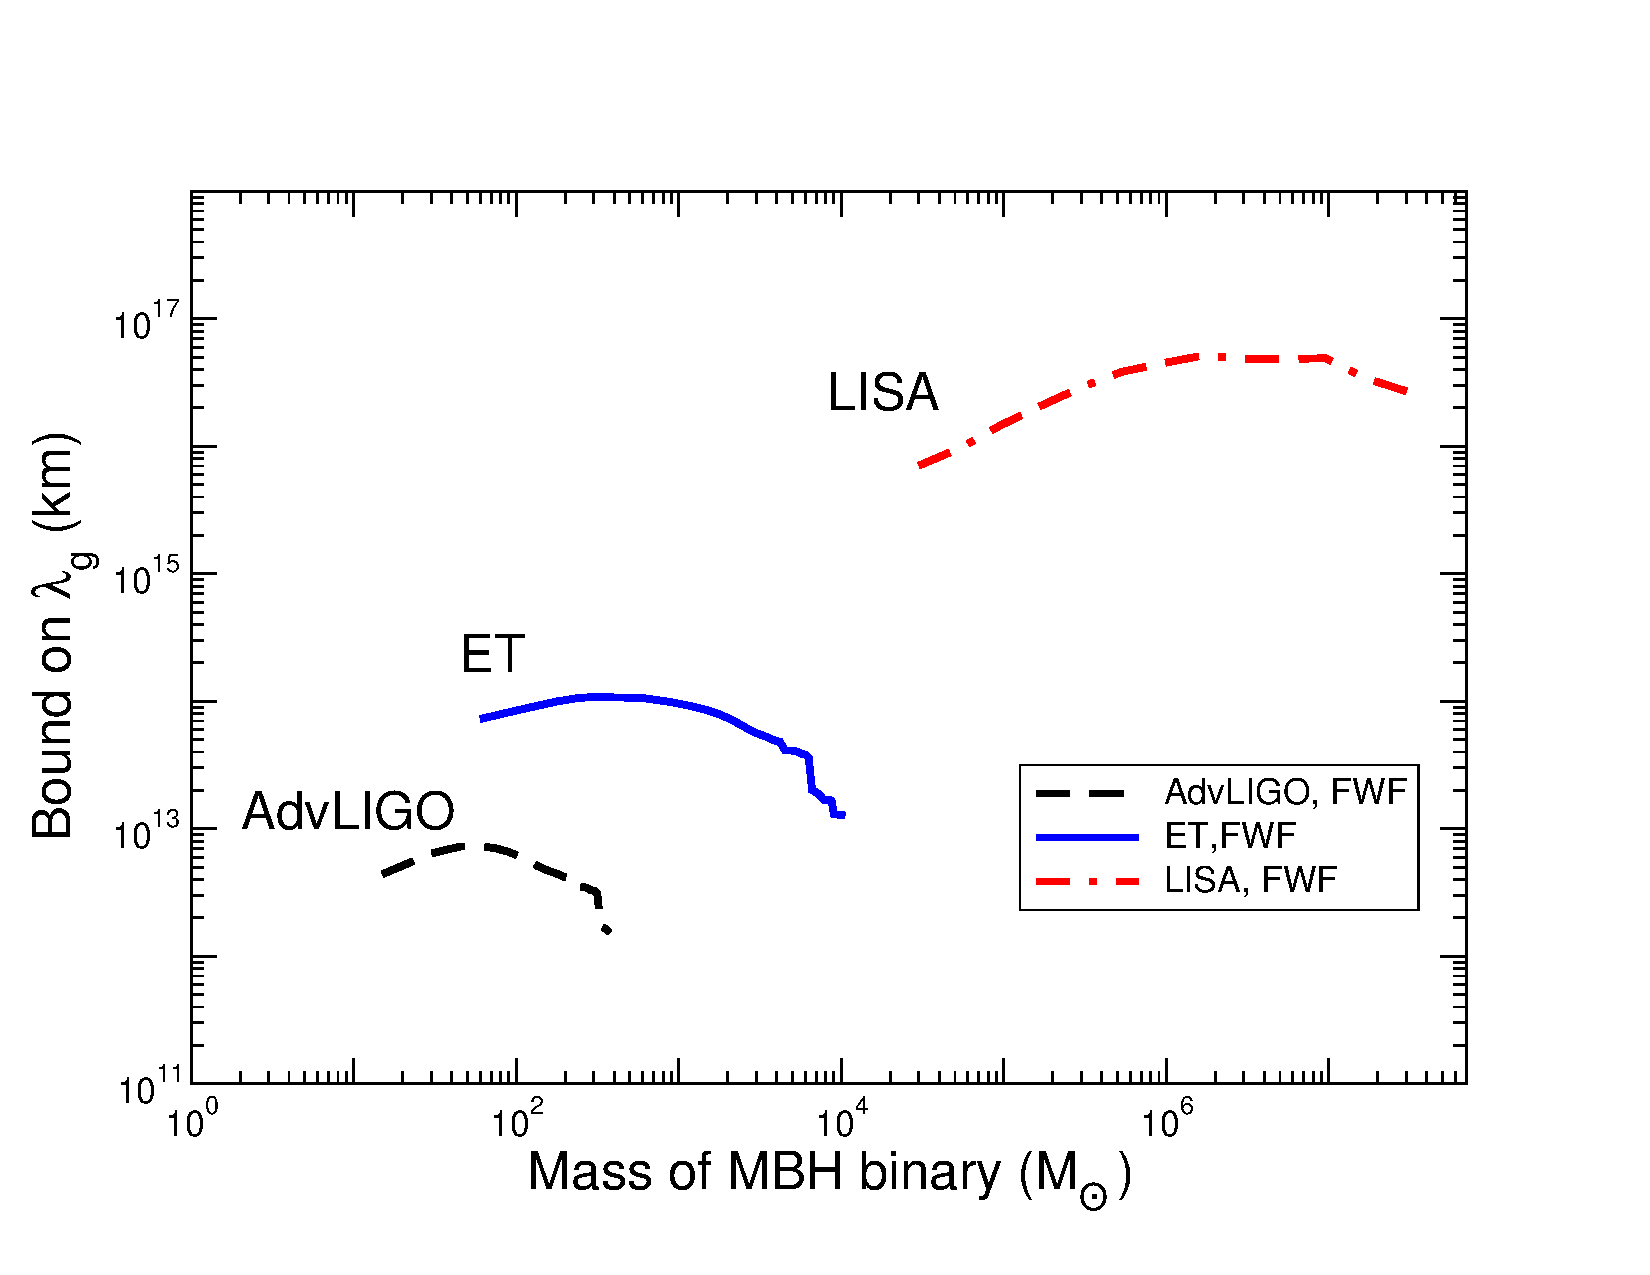
\includegraphics[scale=0.29]{./Sec_ET_ScienceCase/AdvLIGO-ET-LISA_MassiveGraviton.pdf}
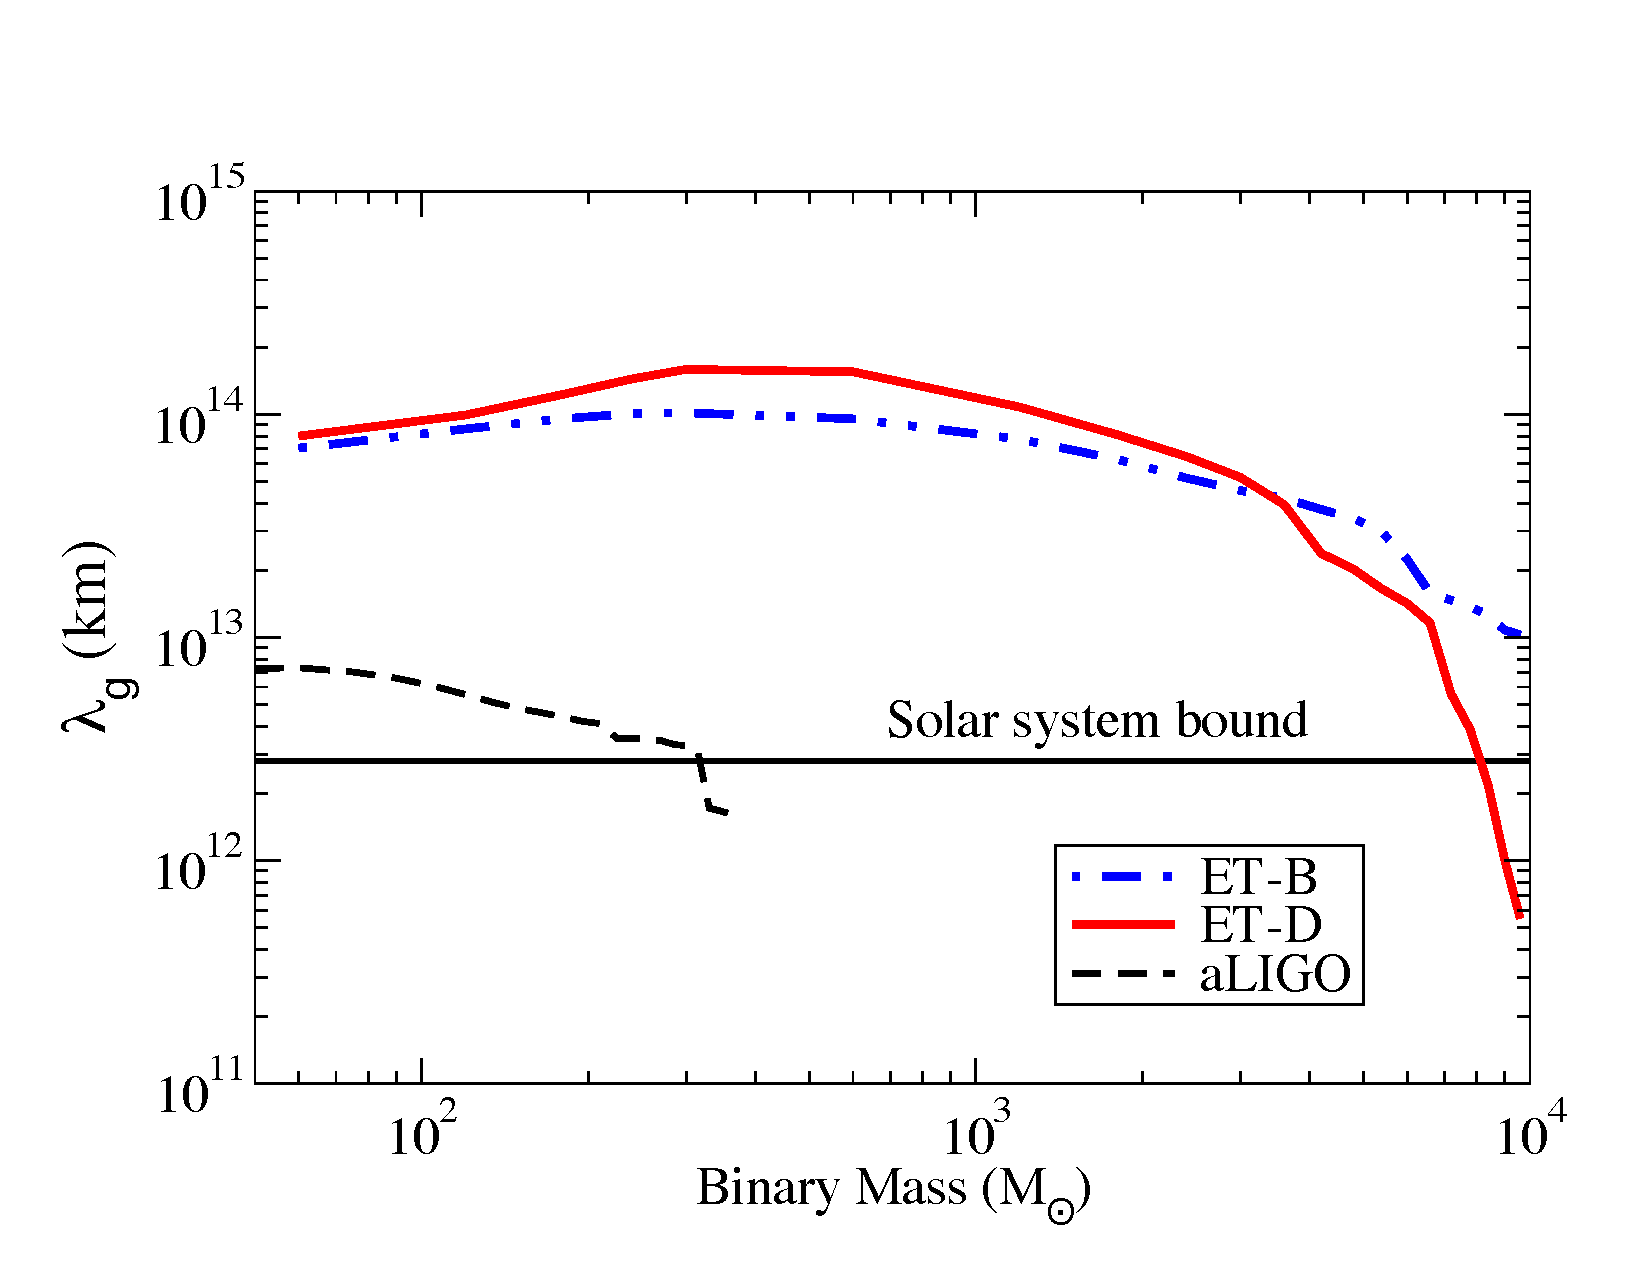
\includegraphics[width=0.49\textwidth]{./Sec_ET_ScienceCase/ET-BnD_MG_1Hz_Massratio2.pdf}
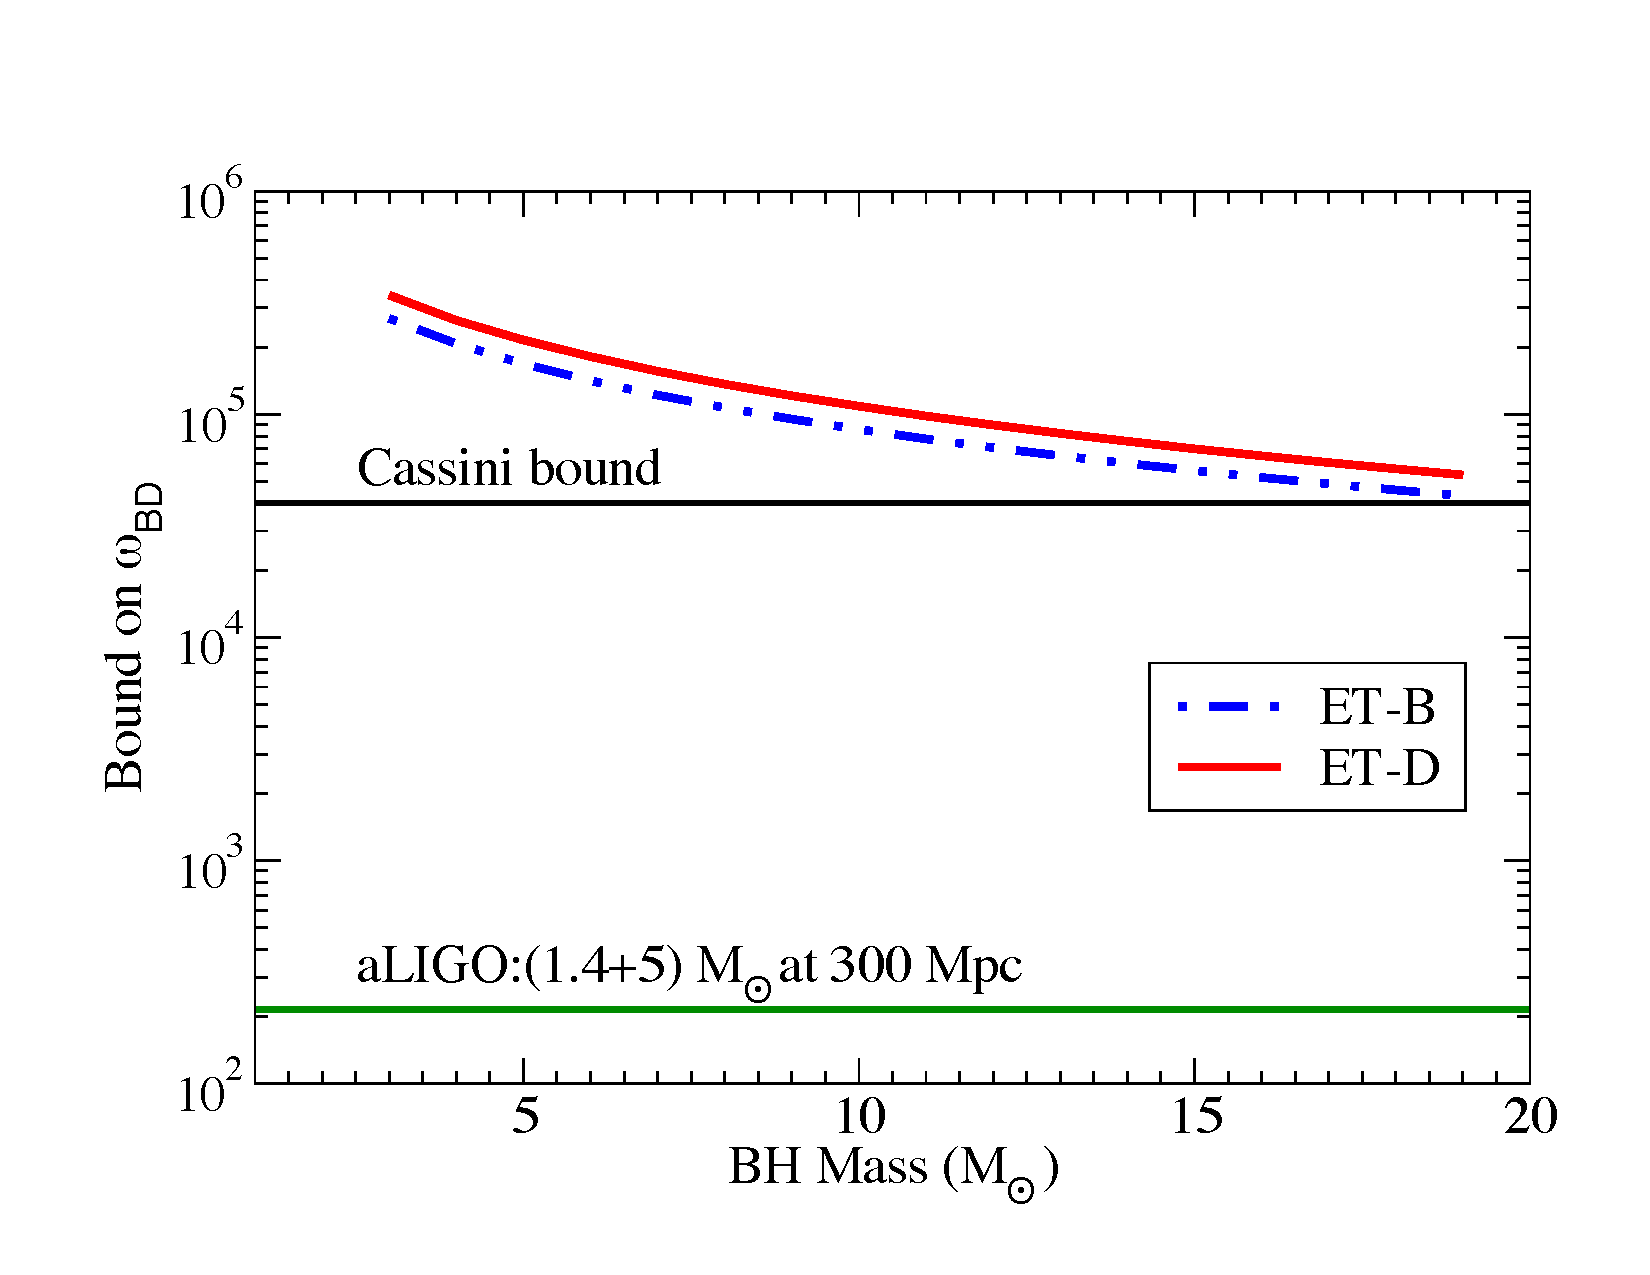
\includegraphics[width=0.49\textwidth]{./Sec_ET_ScienceCase/OmegaBD_1Hz_BH_Mass.pdf}
\caption{
\emph{Left panel:} Bounds on the graviton Compton wavelength that can be
deduced with ET-B and ET-D sensitivity curves as function of the 
total mass of the binary.  The mass ratio for all sources is taken to be 2.
ET can beat the current solar system bound by up to two orders of magnitude.
The limit is independent of the distance to the binary as long as the SNR is
large enough for the Fisher matrix calculation to be reliable. 
\emph{Right:} Bounds on the Brans-Dicke parameter ($\omega_{BD}$) as a function
of the total mass of the NSBH binary observed. For all systems, the NS mass 
is assumed to be 1.4\,$M_\odot.$  The existing bound from the Cassini 
experiment and the possible bounds from aLIGO are also shown.}
\label{fig:MassGravAll}
\end{figure}

The basic idea is simple: if there is a mass associated with the propagation 
of GWs (``a massive graviton''), then the speed of propagation $v_g$ will depend 
on the wavelength $\lambda$ as (in units $c=1$)
$v_g \approx 1 - (\lambda/\lambda_g)^2$, where 
$\lambda_g$ is the Compton wavelength of the graviton, in the limit where 
$\lambda \ll \lambda_g$.  Irrespective of the nature of the alternative 
theory that predicts a massive graviton, 
%(and notwithstanding the difficulties in defining such theories free of 
%pathologies such as the ZvDV discontinuity~\cite{Zakharov70,Veltman70})
it is reasonable to expect the differences between such a hypothetical theory 
and GR in the predictions for the evolution of compact 
binaries to be of order $(\lambda/\lambda_g)^2$. This quantity will be very 
small, given that close to merger $\lambda \sim 10^3$\,km for stellar mass 
BBH, BNS and NSBH inspirals and $\lsim 10^5$\,km for binary IMBH inspirals.

As a result, the gravitational waveform seen by an observer near to a
source will be very close to that predicted by GR.
However, as seen by a detector at a distance $D$, hundreds 
of Mpc away, the phasing of the signal will be distorted because of 
the shifted times-of-arrival, $\Delta t \sim D(\lambda/\lambda_g)^2,$ 
of the waves emitted with different wavelengths during the inspiral.   
In addition to measuring the astrophysical parameters of the system, 
such as masses and spins, the matched filtering technique permits one 
to estimate or bound such effects.

Bounds based on observations of BBH by ET have now been computed~\cite{AW09}. 
%The signal model comprises amplitude-corrected, general relativistic 
%waveforms which are 3PN accurate in amplitude~\cite{BIWW96,ABIQ04,BFIS08,Broeck2007}
%and 3.5PN accurate in phasing~\cite{Blanchet1995,BFIJ02,B96,BDEI04,DIS01,DIS02}.  
%The component stars are assumed to be non-spinning.
%Previous calculations used waveforms which are of Newtonian order in amplitude
%and 2PN order in phase.  As opposed to the Newtonian waveforms, the 3PN 
%amplitude-corrected waveforms contain eight harmonics of the oribtal phase
%$\Psi$ from $\Psi$ up to $8 \,\Psi$, the leading quadrupole component being 
%$2\Psi$.
%The effect of a massive graviton was included in the expression for the 
%orbital phase following Ref.~\cite{bss:will.98}.  
The wavelength-dependent 
propagation speed changes the arrival time $t_a$ of a wave of a given emitted 
frequency $f_e$ relative to that for a signal that propagates at the speed 
of light; that time is given, modulo constants, by
\begin{equation}
t_a = (1+z) \left [ t_e + \frac{D}{2\lambda_g^2 f_e^2} \right ] \,.
\label{time}
\end{equation}
Here $f_e$ and $t_e$ are, respectively, the wave frequency and time of 
emission as measured at the emitter; $z$ is the cosmological redshift, and
\begin{equation}
D \equiv \frac{(1+z)}{a_0}\int_{t_e}^{t_a} a(t) dt \,,
\label{D}
\end{equation}
where $a_0=a(t_a)$ is the present value of the scale factor\footnote{For 
$z\ll1$, $D$ is the same as the luminosity distance $D_{\rm L}$. Hence one 
can take $D\simeq D_{\rm L}$ in the case of ET for which sources considered 
are at 100 Mpc.}.  
%In the frequency domain, this adds a term to 
%the phase $\psi(f)$ of the Fourier transform of the waveform given by 
%$\Delta \psi(f) = -\pi D/f_e \lambda_g^2$.   Then, for each harmonic of the 
%waveform with index $k$, one adds the term
%\begin{equation}
%\Delta \psi_k (f) = \frac{k}{2} \Delta \psi(2f/k) = - \frac{k^2}{4} \pi  D/f_e \lambda_g^2 \,.
%\label{phaseterm}
%\end{equation}
%Here $k=2$ denotes the dominant quadrupole term, with phase $2\Psi$, $k=1$ denotes the term with phase $\Psi$, $k=3$ denotes the term with phase $3\Psi$, and so on.
%
This is an ad-hoc procedure
because a massive graviton theory will undoubtedly deviate from GR not 
just in the propagation of GW, but also in the way GW damping affects 
the phase and the amplitudes of the emitted radiation.  
% If, for example, such a theory introduces a leading correction to the 
% quadrupole phasing $\psi_{\rm quad} \sim (\pi {\cal M} f_e)^{-5/3}$ of 
% order $(\lambda/\lambda_g)^2 \times (\pi {\cal M} f_e)^{-5/3}$, where 
% $\cal M$ is the chirp mass, then the propagation induced phasing term 
% (\ref{phaseterm}) will be larger than this correction term by a factor 
% of order $k^2 (D/{\cal M})(\pi {\cal M} f_e)^{8/3} \sim (D/{\cal M})v^8$.  
% Since $v \sim 0.1$ for the important part of the binary inspiral, and 
% $D \sim$ hundreds of Mpc. 
However, it turns out that hundreds of Mpc away from the source,
the propagation effect will dominate over wave generation effects \cite{AW09}.  
In any case, given the fact that there is no generic theory of a massive 
graviton, there is no choice but to omit these unknown contributions.

Estimates of the bounds on the massive graviton parameter are based
on the Fisher matrix formalism,  
% We construct the Fisher matrix for the different
% detector noise PSDs using the amplitude corrected PN waveform model
% described earlier, converted to the
% Fourier domain using the stationary phase approximation.
which used a six-dimensional parameter space consisting of the time 
and phase ($t_c, \, \phi_c$) of coalescence, the chirp mass ${\cal M}$, 
the mass asymmetry parameter $\delta=|m_1-m_2|/(m_1+m_2)$, the massive 
graviton parameter $\beta_g=\pi^2 D {\cal M}/\lambda_g^2(1+z)$, 
and the luminosity distance $D_{\rm L}$.  
%We fix the three angles, $\theta$, $\phi$ and $\psi$  which appear in the antenna pattern functions to be $\pi/3$, $\pi/6$ and $\pi/4$ respectively and the inclination angle of the binary to be $\iota=\pi/3$.
 % Details of the Fisher matrix approach as applied to the compact binary coalescence signals can be found in Refs.~\cite{Cutler:1994ys,PoissonAndWill,Arun:2005}, and more recently
% in Ref.~\cite{Vallisneri:2007ev}, which critically re-examines the caveats involved in
% using the Fisher matrix formalism to deduce error bounds for various GW detector configurations.

% The square root of each of the diagonal entries in the inverse of the Fisher matrix gives a lower bound
% on the error covariance of any unbiased estimator.  Our focus here is solely
% on the diagonal element corresponding to the massive graviton parameter.  
%The $1-\sigma$ error bar on $\beta_g$ can be translated into a bound on the
%Compton wavelength using $\Delta \beta_g=\beta_g$, and this is the quantity
%that we use in the plots as well as in the discussions.

Figure~\ref{fig:MassGravAll}, left panel, plots the bound on the Compton 
wavelength as a function of the total mass of the system.  The bound plotted is
the 1-sigma error in the measurement accuracy of the parameter $\lambda_g.$
For both choices of sensitivity, ET-B and ET-D, the bound will improve 
beyond that set by solar system experiments by some two orders-of-magnitude. 

The bounds are, in principle, more or less independent of the distance:
sources at greater distances will have smaller SNRs but such signals suffer
larger dispersion as they propagate greater distances. Hence the overall 
effect is more or less the same irrespective of the distance to source.  
However, for very large distances the SNR may not be high enough for 
the Fisher matrix estimate to be reliable. With the accumulation of
sources, the bound can be further improved by $\sqrt{N},$ where $N$
is the number of sources detected. Since ET will observe millions of compact 
binary coalescences, it has the potential to improve the bounds by
several orders of magnitude more than that shown in Fig.\,\ref{fig:MassGravAll}.
%We assume the binaries to be nonspinning and use a waveform which
%is 3.5PN accurate in the phase and 3PN in amplitude. Due to the inclusion of
%PN terms in the amplitude, one gets better bounds due to the presence of
%higher harmonics.

\subsubsection{Bounds on Brans-Dicke parameter}
% \ledby{Arun: June 11th}\\

The Brans-Dicke (BD) theory \cite{BransDicke61} is an alternative theory
of gravity that has an additional scalar field, which couples to matter,
as well as the tensor field of GR.
The coupling of the scalar field is described by a dimensionless parameter
$\omega_{BD}$; in the limit $\omega_{BD}\rightarrow\infty$ the theory 
goes over to GR.  Since scalar-tensor field  theories predict dipolar 
gravitational radiation, this parameter is also a measure of the dipolar 
GW content.

The best bound on this parameter so far has come from the solar
system experiment \emph{Cassini}, by measuring the frequency shift of radio
signals to and from the spacecraft as it orbited near the sun~\cite{Cassini}.
The resulting lower limit on $\omega_{BD}$ is about $4\times10^{4}$.

Gravitational wave observations can also put interesting bounds on $\omega_{BD}$
\cite{WillBD94,KKS95}. This is possible because
the GW phasing formula in BD theory is the same as in GR except
for an additional dipolar term proportional to $\omega_{BD}^{-1}$.
Hence it is possible to measure or bound this quantity from GW observations. %(see Refs~\cite{WillBD94,KKS95} for details).
The dipolar content in GW also depends on the internal structure of the compact
body via a quantity called ``sensitivity'' $s_A$ (Sec.\,3.3 of~\cite{Wthexp}).
\begin{equation}
\left(\frac{dE}{dt}\right)_{\rm dipole} \propto {\frac{(s_1-s_2)^2}{\omega_{BD}}}, 
\end{equation}
where $s_1$ and $s_2$ are the sensitivities of the
binary constituents. The sensitivity parameter for a BH is 
$s_{\rm BH} \equiv 0.5$ while that of the NS $s_{\rm NS}$ ranges between $\simeq 0.1$--$0.2$ 
depending on its mass.  Thus, for a BNS $|s_1-s_2| \sim 0.2 \delta M/M_\odot$, 
$\delta M$ being the difference in mass of the two NS, for NSBH 
systems $|s_1-s_2|>0.3$ and for BBH $|s_1-s_2|=0$.
Therefore, for bounding BD theories one of the components of the binary
should be a NS. The bound is also very sensitive to how asymmetric the 
binary component masses are.  The bound that can be placed on $\omega_{BD}$ 
decreases as the asymmetry increases.  Due to these factors, current
GW bounds on $\omega_{BD}$ are very weak, $\sim 5000$ at best~\cite{WillBD94}.

However, if ET has very good low-frequency sensitivity it can achieve more stringent 
limits than the solar system bounds. Figure~\ref{fig:MassGravAll},
right panel, shows the bound on $\omega_{BD}$ obtained using NSBH systems for
ET-D and ET-B.  The NS mass is assumed to be $1.4\,M_{\odot}$ and that of the BH is 
varied from $3\,M_\odot$ to $19\,M_\odot$.  The best bounds would come from 
the observations of NSBH systems with lightest BH mass.
Given that ET's sensitivity extends down to 1\,Hz, (a basic assumption of these
calculations) then the bounds on $\omega_{BD}$ could be as high as $\sim 3\times 10^5$.

\subsubsection{Parametrized tests of post-Newtonian theory}


\begin{figure*}
\centering
%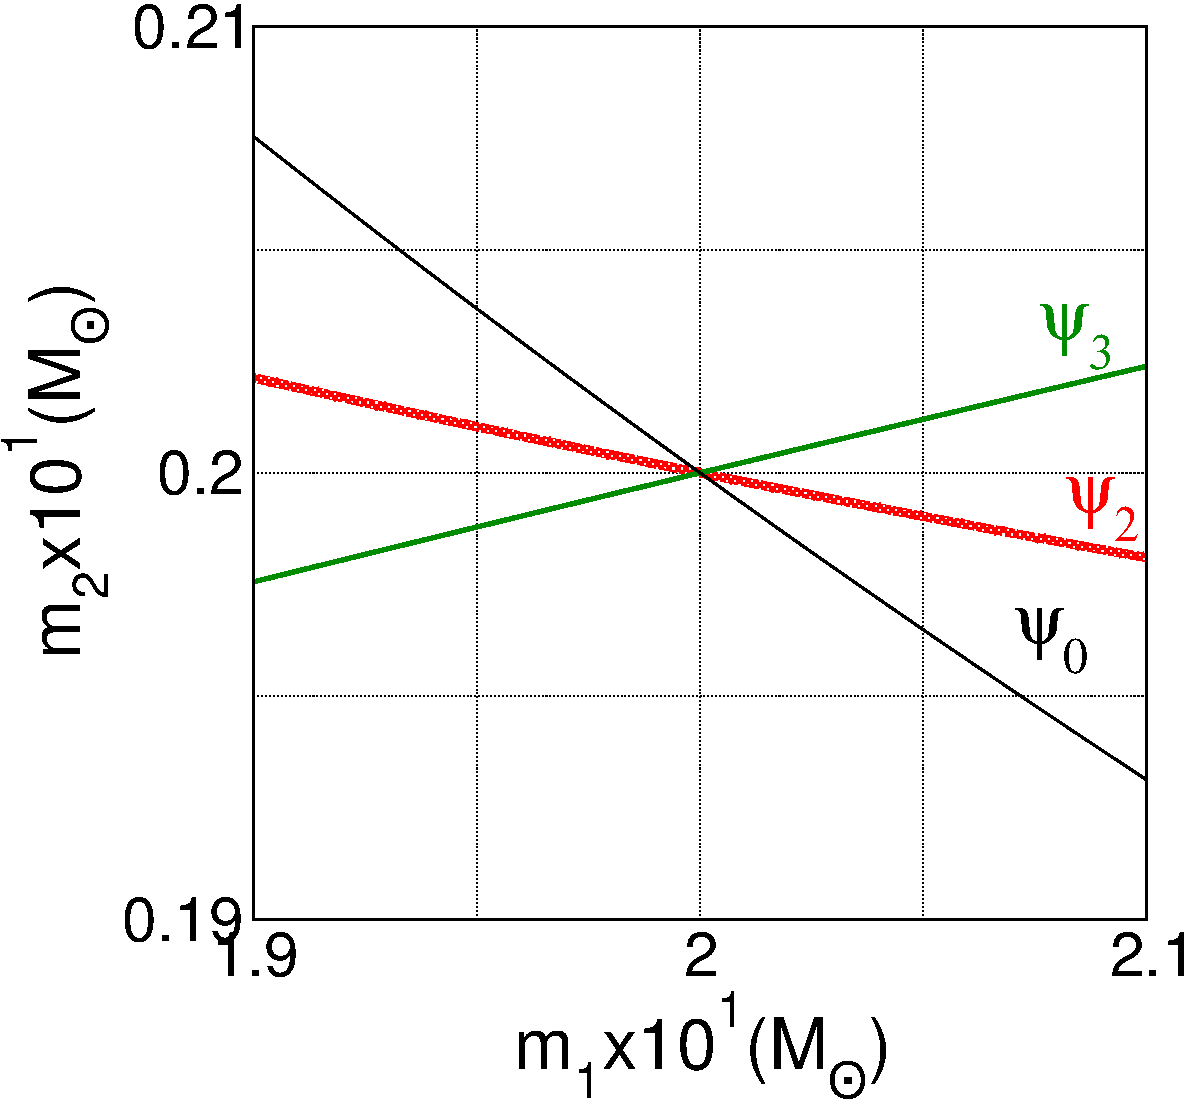
\includegraphics[width=0.34\textwidth]{./Sec_ET_ScienceCase/m1m2_psi3_2e0-2e1.pdf}
%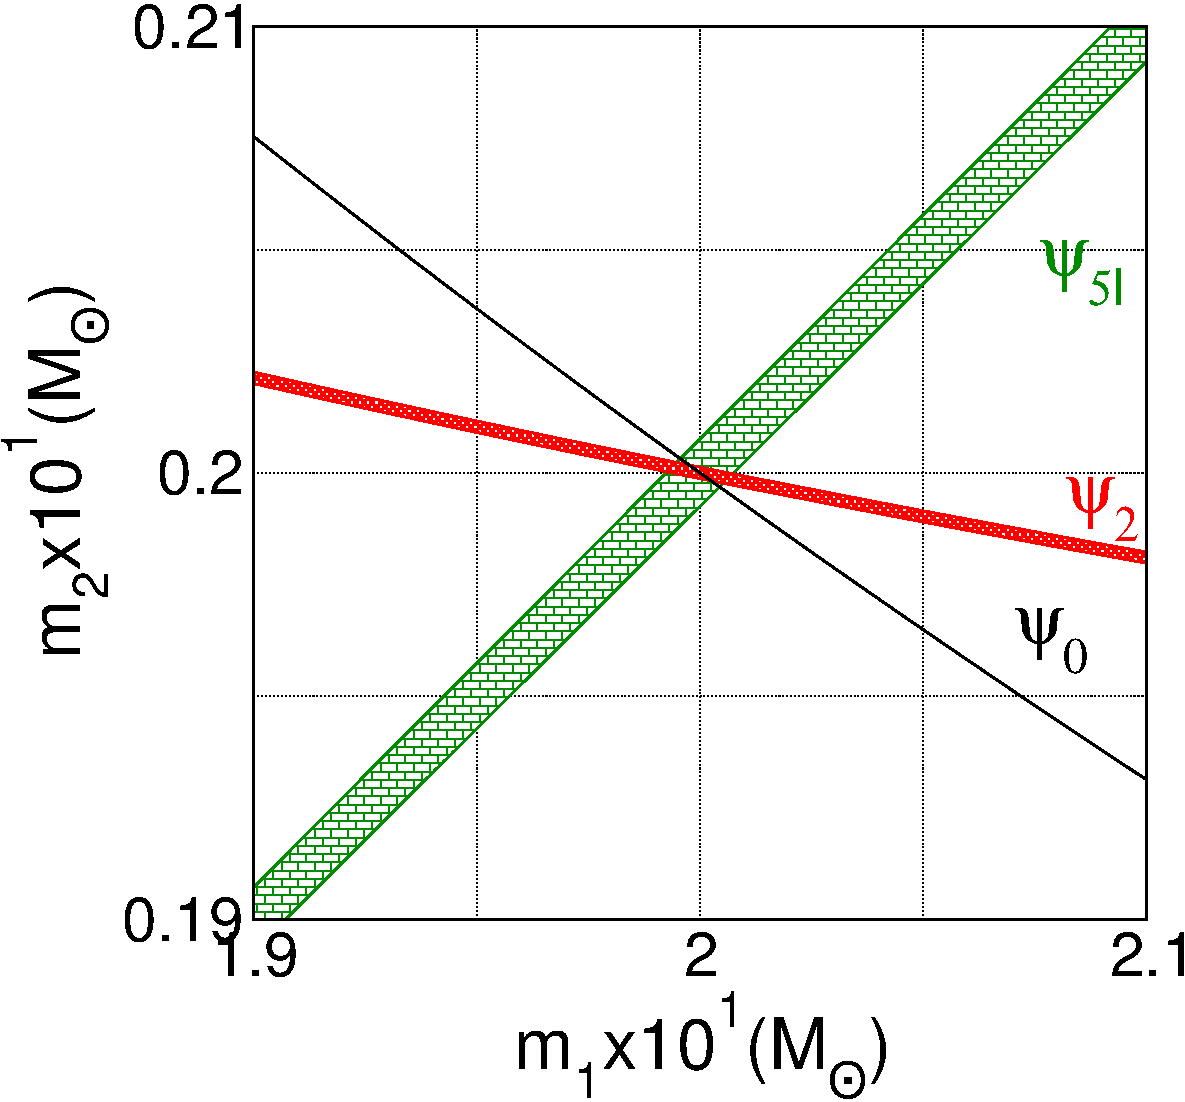
\includegraphics[width=0.45\textwidth]{./Sec_ET_ScienceCase/m1m2_psi5l_2e0-2e1.pdf}
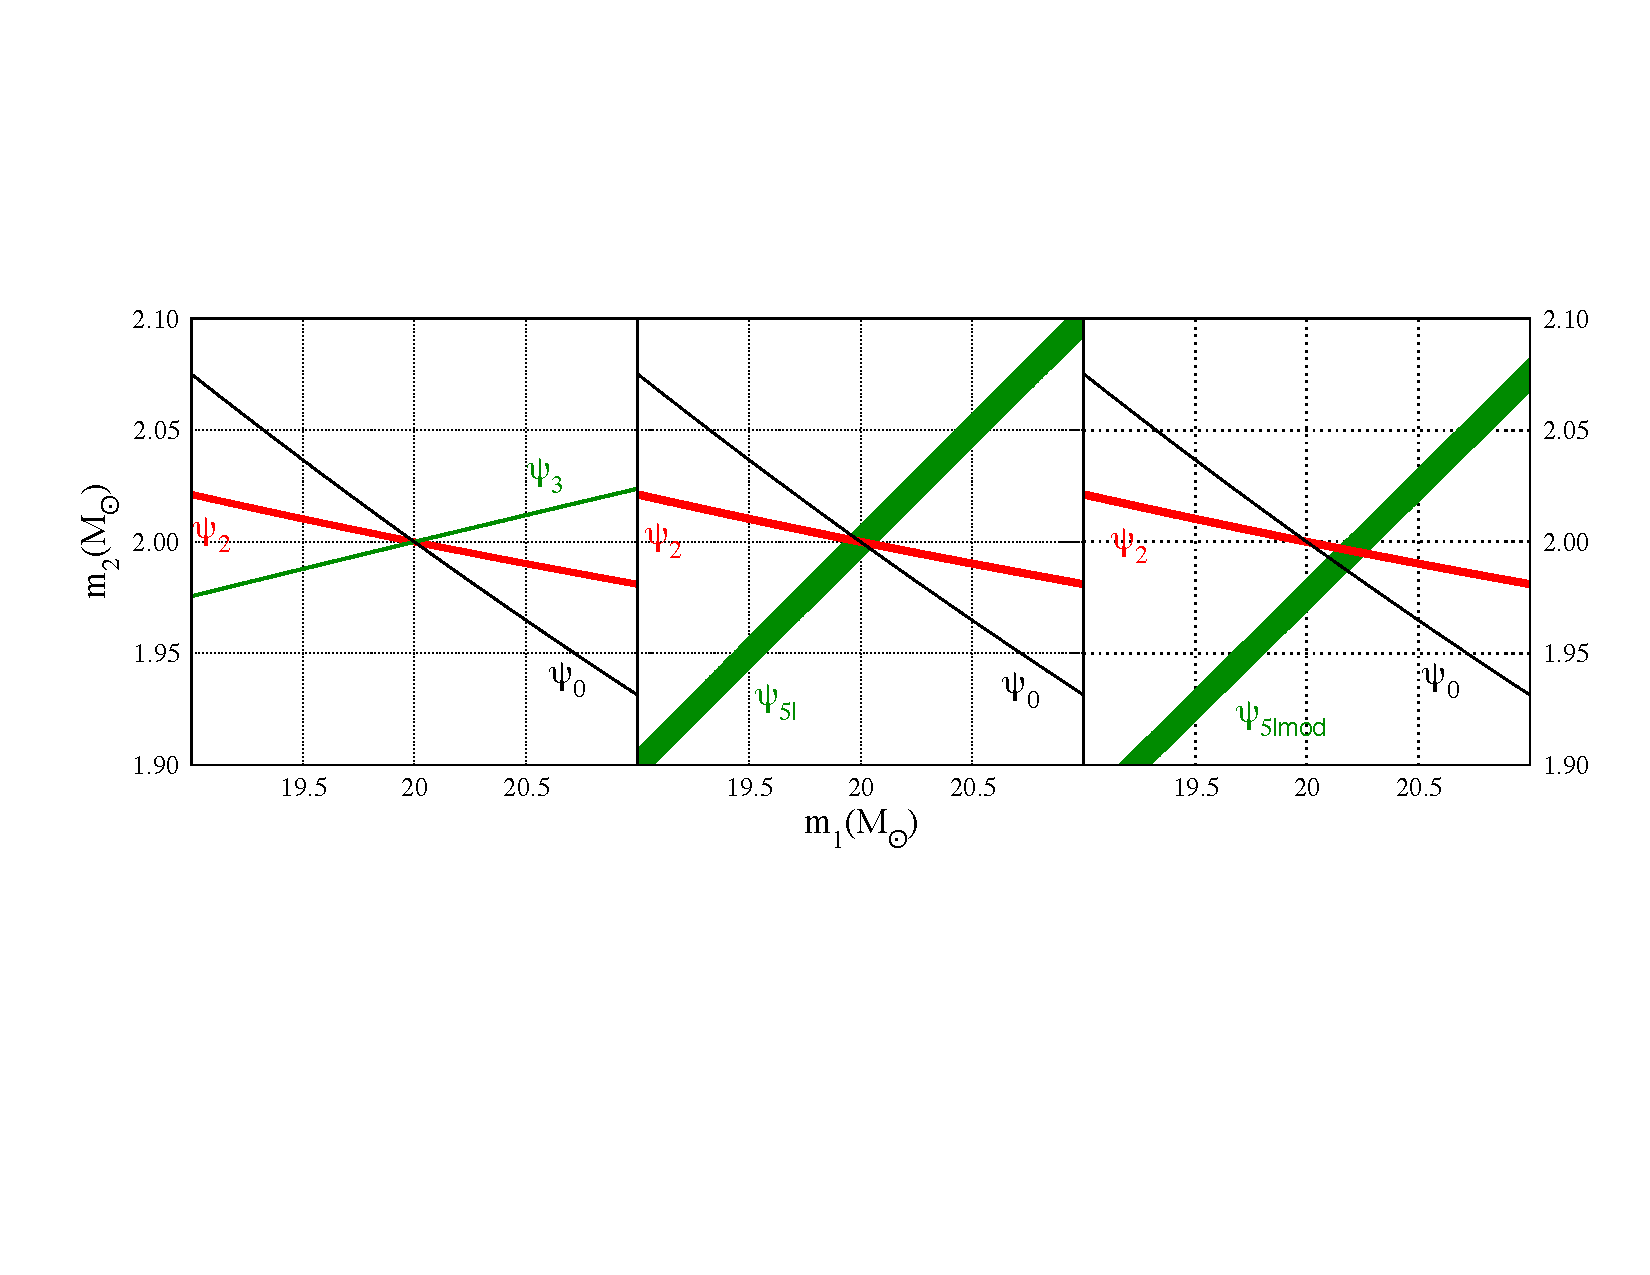
\includegraphics[width=0.95\textwidth]{./Sec_ET_ScienceCase/m1m2_2e02e1_p5lvsp5lmod1p.pdf}

\caption{Curves of constant PN coefficients in the $(m_1,m_2)$ plane 
for a  $(2,20)\,M_\odot$ BBH merger at 300\,Mpc observed in ET-B.  The left 
and middle plots correspond to the case when the post-Newtonian 
coefficients are all as in GR and all three curves intersect at a 
single point. The plot on the right corresponds to the case when the 
measured value of $\psi_{5l}$ differs from GR by 1\% and in this 
case the three curves fail to intersect at a common point.  The
thickness of the lines is the 1-sigma error in the measurement
of the corresponding parameter. \label{fig:m1m2plots}}
\end{figure*}

It is also possible to test for violations of GR without assuming a 
particular alternative model.  One such test was proposed by 
Arun et al.~\cite{testGR:2006,testGR:2007,testGR:2010} and is
based on the post-Newtonian (PN) expansion of the phase of an inspiral 
signal in the frequency domain:
\begin{equation}
\Psi(f) = \sum_{j=0}^7 \left[\psi_j + 
\psi_{jl}\ln(f)\right]\,f^{(j-5)/3},
\label{freqphase}
\end{equation}
where the PN coefficients $\psi_j$ and $\psi_{jl}$,
$j = 0, \ldots, 7$ can be found in \cite{testGR:2010}.
Under the simplifying assumption that spins are zero, these 
coefficients only depend on the component masses $m_1$, $m_2$ of
the binary. Hence only two of these coefficients
are independent, and a possible test of PN theory 
(and hence of GR) is to check for consistency between any three of 
them. Particular attention has been given to $\psi_3$ and $\psi_{5l}$:
\begin{itemize}
\item $\psi_3$ is the lowest-order coefficient which gets contributions from scattering of gravitational
waves off the spacetime near the binary, the so-called tail terms: hence it encapsulates the non-linear
character of GR.
\item $\psi_{5l}$ is the lowest-order coefficient of a logarithmic term in (\ref{freqphase}). General
relativity is not consistent with a simple Taylor expansion.
\end{itemize}
The basic idea of the test is to measure the PN coefficients by fitting the 
observed signal to a model in which three of the PN coefficients, 
instead of two, are treated as independent parameters. As mentioned 
before, each coefficient depends on the two masses $\psi_j=\psi_j(m_1,\,m_2).$
Thus, a measured value of one of the PN coefficients can be used to
draw a curve in the $(m_1,\,m_2)$ plane by inverting the relation
$\psi_j=\psi_j(m_1,\,m_2),$ where the left hand side is the measured value
and the right-hand side is a function only of $m_1, m_2.$ Intersection of
two of the curves, say those corresponding to the measurement of 
$\psi_0$ and $\psi_2$ ($\psi_1$ is identically zero in GR),
gives the component masses. If GR is the correct theory then the curve 
$\psi_3=\psi_3(m_1,\,m_2)$ (left panel of Fig.\,\ref{fig:m1m2plots}) or
$\psi_{5l}=\psi_{5l}(m_1,\,m_2)$ (middle panel of the figure)
will pass through the intersection of the curves corresponding
to $\psi_0$ and $\psi_2.$ If, however, GR is not the correct theory of 
gravity and, say, the value of $\psi_{5l}$ is different from 
that in GR then the curve $\psi_{5l} = \psi_{5l}(m_1,\,m_2)$ will 
not pass through the intersection of the other two curves as in the 
right panel of Fig.\,\ref{fig:m1m2plots}.

In this way, ET will be able to test the non-linear predictions of GR
and confirm whether GR is the correct theory when the gravitational field
becomes so strong that orbital speeds get close to the speed of light.
No other experiments or observations conceived so far can test GR to
such a high order in PN theory.
%The sensitivity at low frequency can have a dramatic effect on the ability to test GR, as shown in Fig.~\ref{fig:lowfreq_testGR}.

%\begin{figure}[h!]
%\centering
%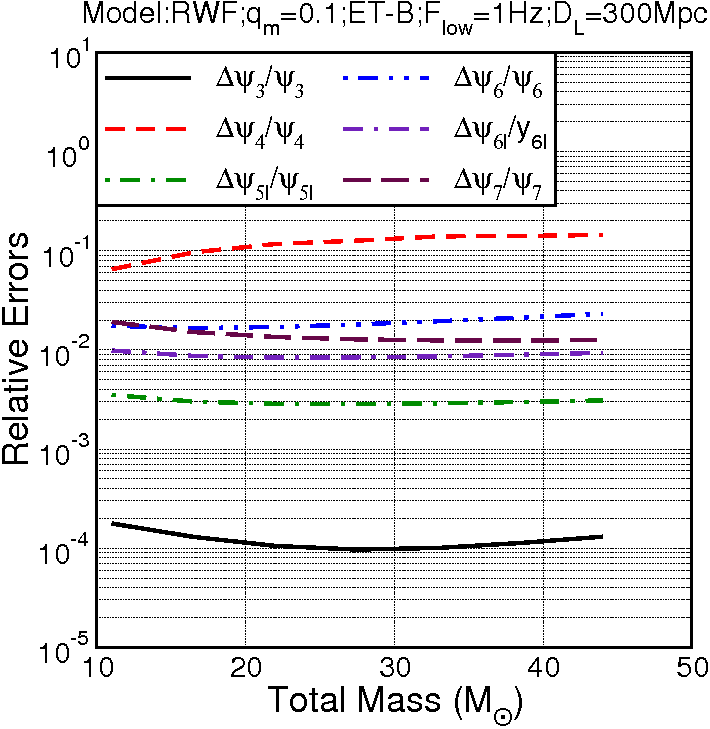
\includegraphics[width=0.45\textwidth]{./Sec_ET_ScienceCase/Errvsmass_RWF_1Hz_0p1_300Mpc.png}
%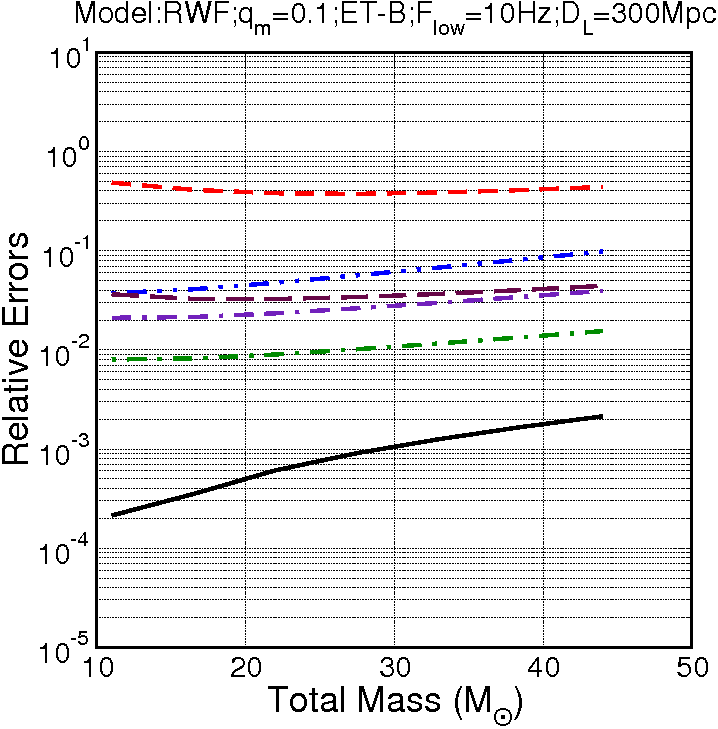
\includegraphics[width=0.45\textwidth]{./Sec_ET_ScienceCase/Errvsmass_RWF_10Hz_0p1_300Mpc.png}
%\caption{Varying the lower frequency cut-off can affect the accuracy in measuring phase coefficients by factors of several
%to an order of magnitude. On the left are relative errors with a 1 Hz cut-off, on the right with a 10 Hz cut-off.}
%\label{fig:lowfreq_testGR}
%\end{figure}


%% \subsection{Test of gravity - 1}
%% \ledby{Bala}

%% \subsection{Test of gravity - 2}
%% \ledby{Bala}
\subsubsection{Measuring the dark energy equation of state
and its variation with $z$}
% \ledby{Van Den Broeck}

Over the past decade, evidence has emerged suggesting that the expansion of the Universe is accelerating. Possible explanations include a failure of general relativity at large length scales, a cosmological constant in the Einstein equations, or a new contributor to the mass/energy content of the Universe called dark energy (DE) (see \cite{PeeblesRatra03} for a review). Assuming a homogeneous and isotropic Universe, DE can be characterized by an EoS of the form $p_{\rm DE} = w(z) \rho_{\rm DE}$, where $p_{\rm DE} < 0$ and $\rho_{\rm DE} > 0$ are the pressure and density, respectively. If the EoS parameter $w(z)$ is constant and equal to $-1$ then this corresponds to having a positive cosmological constant in the gravitational field equations. Current constraints allow for this possibility, but other possibilities are not ruled out. The seven year WMAP data combined with Type Ia supernova measurements and baryon acoustic oscillations in the galaxy distribution lead to the constraint $w = -1.10 \pm 0.14$ at the 68\% confidence level \cite{WMAP7}.

The GW signal from inspiraling compact binaries is particularly ``clean" and well-understood. Consequently, as suggested by Schutz, one can think of using inspiral events as ``standard sirens", much in the way Type Ia supernovae have been used as standard candles \cite{Schutz86}. From the GW signal itself the luminosity distance $D_{\rm L}$ can be inferred, but not the redshift. However, if a particular compact binary coalescence event is accompanied by a sufficiently distinct electromagnetic counterpart, then it will be possible to find its position in the sky, identify the host galaxy, and obtain the redshift $z$. The relationship $D_{\rm L}(z)$ depends sensitively on cosmological parameters such as the Hubble constant at the current epoch $H_0$, the normalized matter and DE densities $\Omega_{\rm M}$ and $\Omega_{\rm DE}$, and the DE EoS parameter $w$. For example, in a spatially flat FLRW Universe and assuming a constant $w$,
\begin{equation}
D_{\rm L}(H_0, \Omega_{\rm M}, \Omega_{\rm DE}, w; z) = (1+z)\,\int_0^z \frac{dz'}{H_0 \left[ \Omega_{\rm M}(1+z')^3 + \Omega_{\rm DE} (1+z')^{3(1+w)} \right]^{1/2}}.
\label{DLgeneral}
\end{equation}
The intrinsic luminosity, and hence the luminosity distance, of an inspiral GW event can be inferred directly from the amplitude of the observed waves and from the component masses, which govern the structure of the signal. Thus, unlike Type Ia supernovae, their calibration does not depend on the brightness of other sources. Thus GW astronomy opens up the possibility of cosmography \emph{without having to rely on the lower rungs of the cosmic distance ladder}.

Compact binary coalescences that involve a NS are assumed to have strong electromagnetic counterparts, mostly in the form of strongly beamed gamma radiation directed perpendicularly to the plane of the inspiral. Such events are believed to be the progenitors of short, hard Gamma Ray Bursts (GRBs): if the beam roughly points towards Earth then a flash of gamma radiation is seen, followed by an afterglow in the lower-frequency electromagnetic spectrum.
This would then allow us to identify the host galaxy and obtain a redshift.

The GW signal from a NSBH coalescence will be visible out to $z = 3.5$. Within the corresponding volume, it is reasonable to expect $\sim 10^4$ or more such coalescences per year, but depending on the opening angle of the gamma ray beam only a few percent of these will be visible as a GRB. Hence we should have a few hundred sources at our disposal for which the redshift can be measured. The uncertainty on $z$ will be negligibly small, while $D_{\rm L}$ will be measurable with $\sim 3$\% inaccuracy at $z = 1$, rising to $\sim 10$\% at $z = 3.5$. Fitting the measured values of $D_{\rm L}$ against redshift by varying $H_0$, $\Omega_{\rm M}$, $\Omega_{\rm DE}$, and $w$ in the relationship (\ref{DLgeneral}) should then allow for the determination of these cosmological parameters with uncertainties of 5\% or better, as discussed further in Section~\ref{cosmo_parameters}.

\subsubsection{Testing the uniqueness theorem of black hole spacetimes}
\label{subsubsec:uniquenesstheorem}
It is generally accepted that the compact objects observed in 
the centres of most galaxies are massive, rotating BHs described by 
the Kerr metric of GR. This belief comes in part from the uniqueness 
theorem, which states that the Kerr metric is the unique end state 
of gravitational collapse~\cite{carter71}. However, this theorem is 
based on several assumptions -- the spacetime is vacuum, axisymmetric 
and stationary; there is a horizon in the spacetime; and there are no 
closed timelike curves. If one of these assumptions were violated, 
then objects that deviate from the Kerr metric could exist.
\begin{figure}
\centering
\begin{tabular}{|c|c|}
\hline
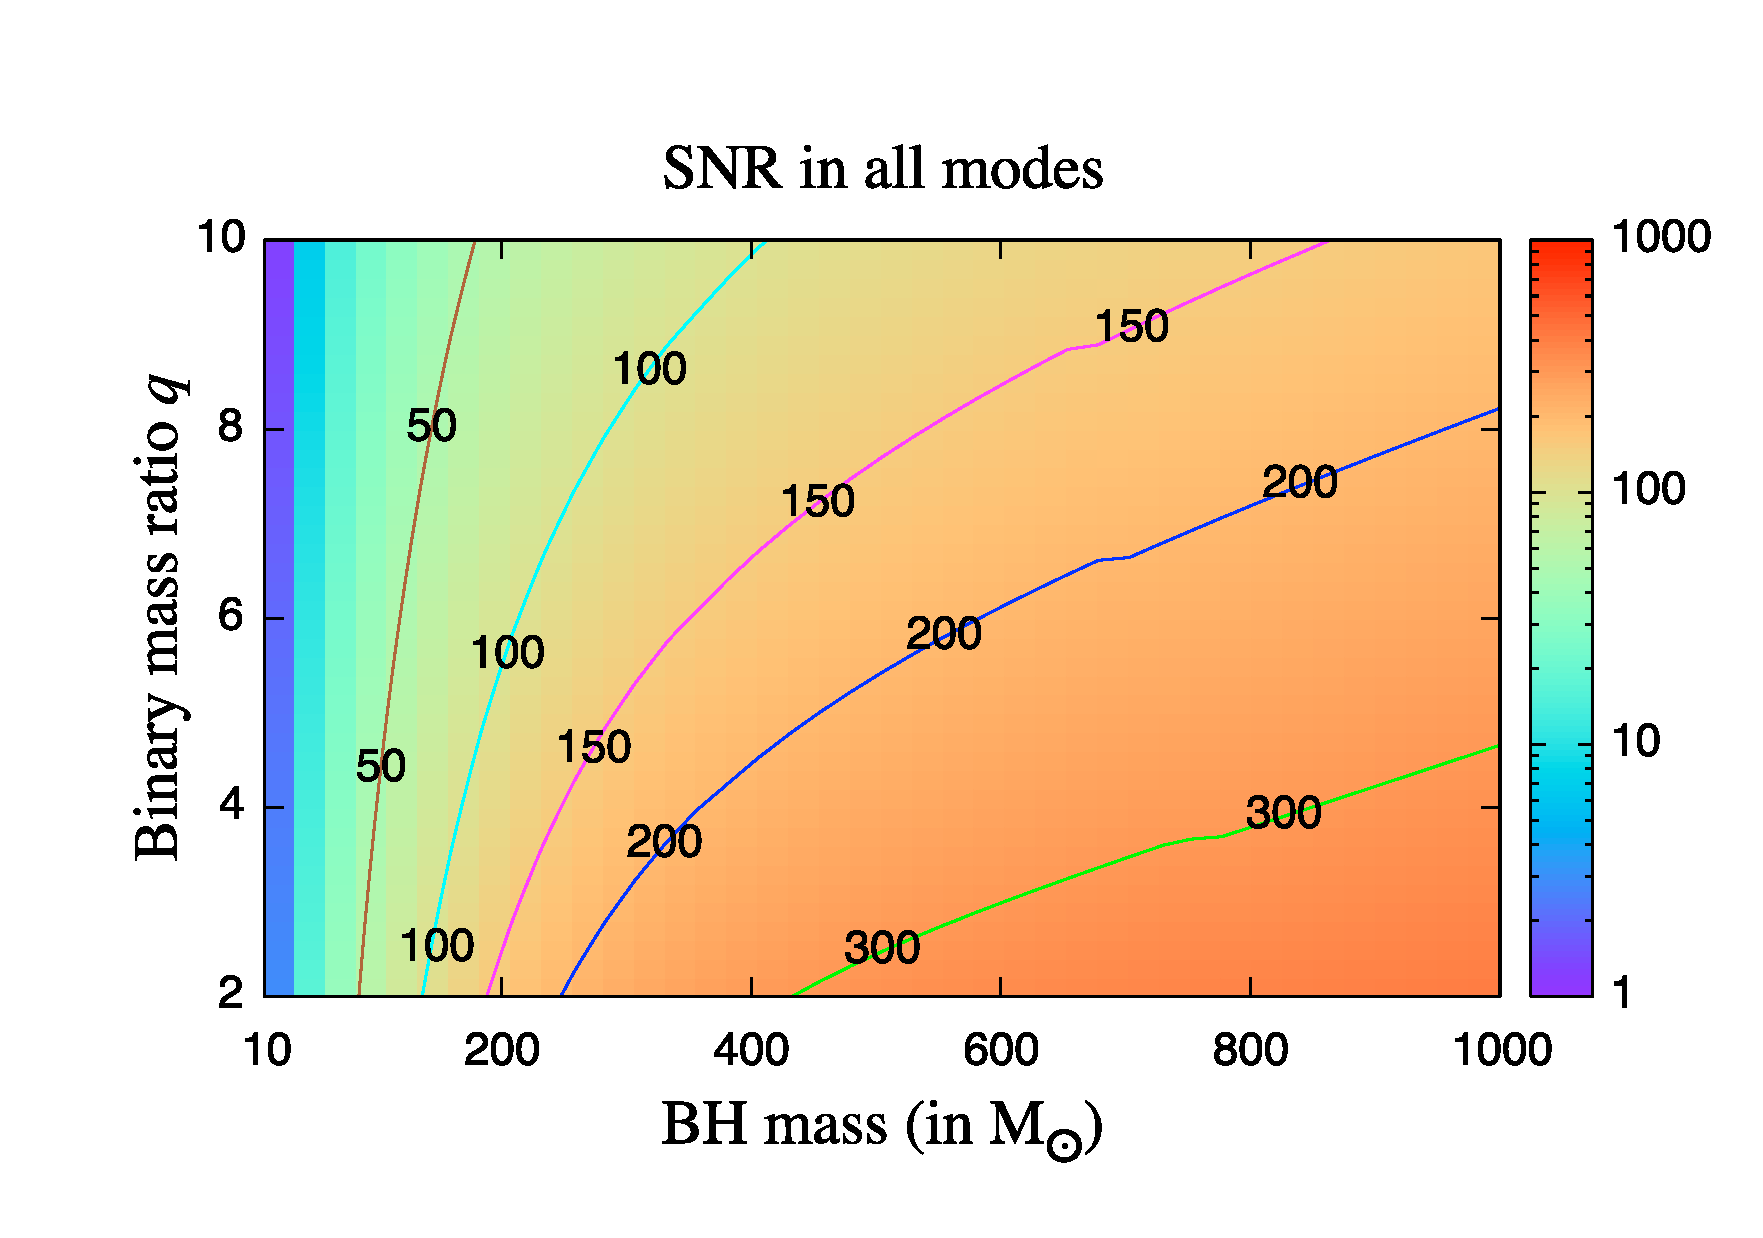
\includegraphics[width=0.45\textwidth]{./Sec_ET_ScienceCase/ET-SNR-all.pdf}  &
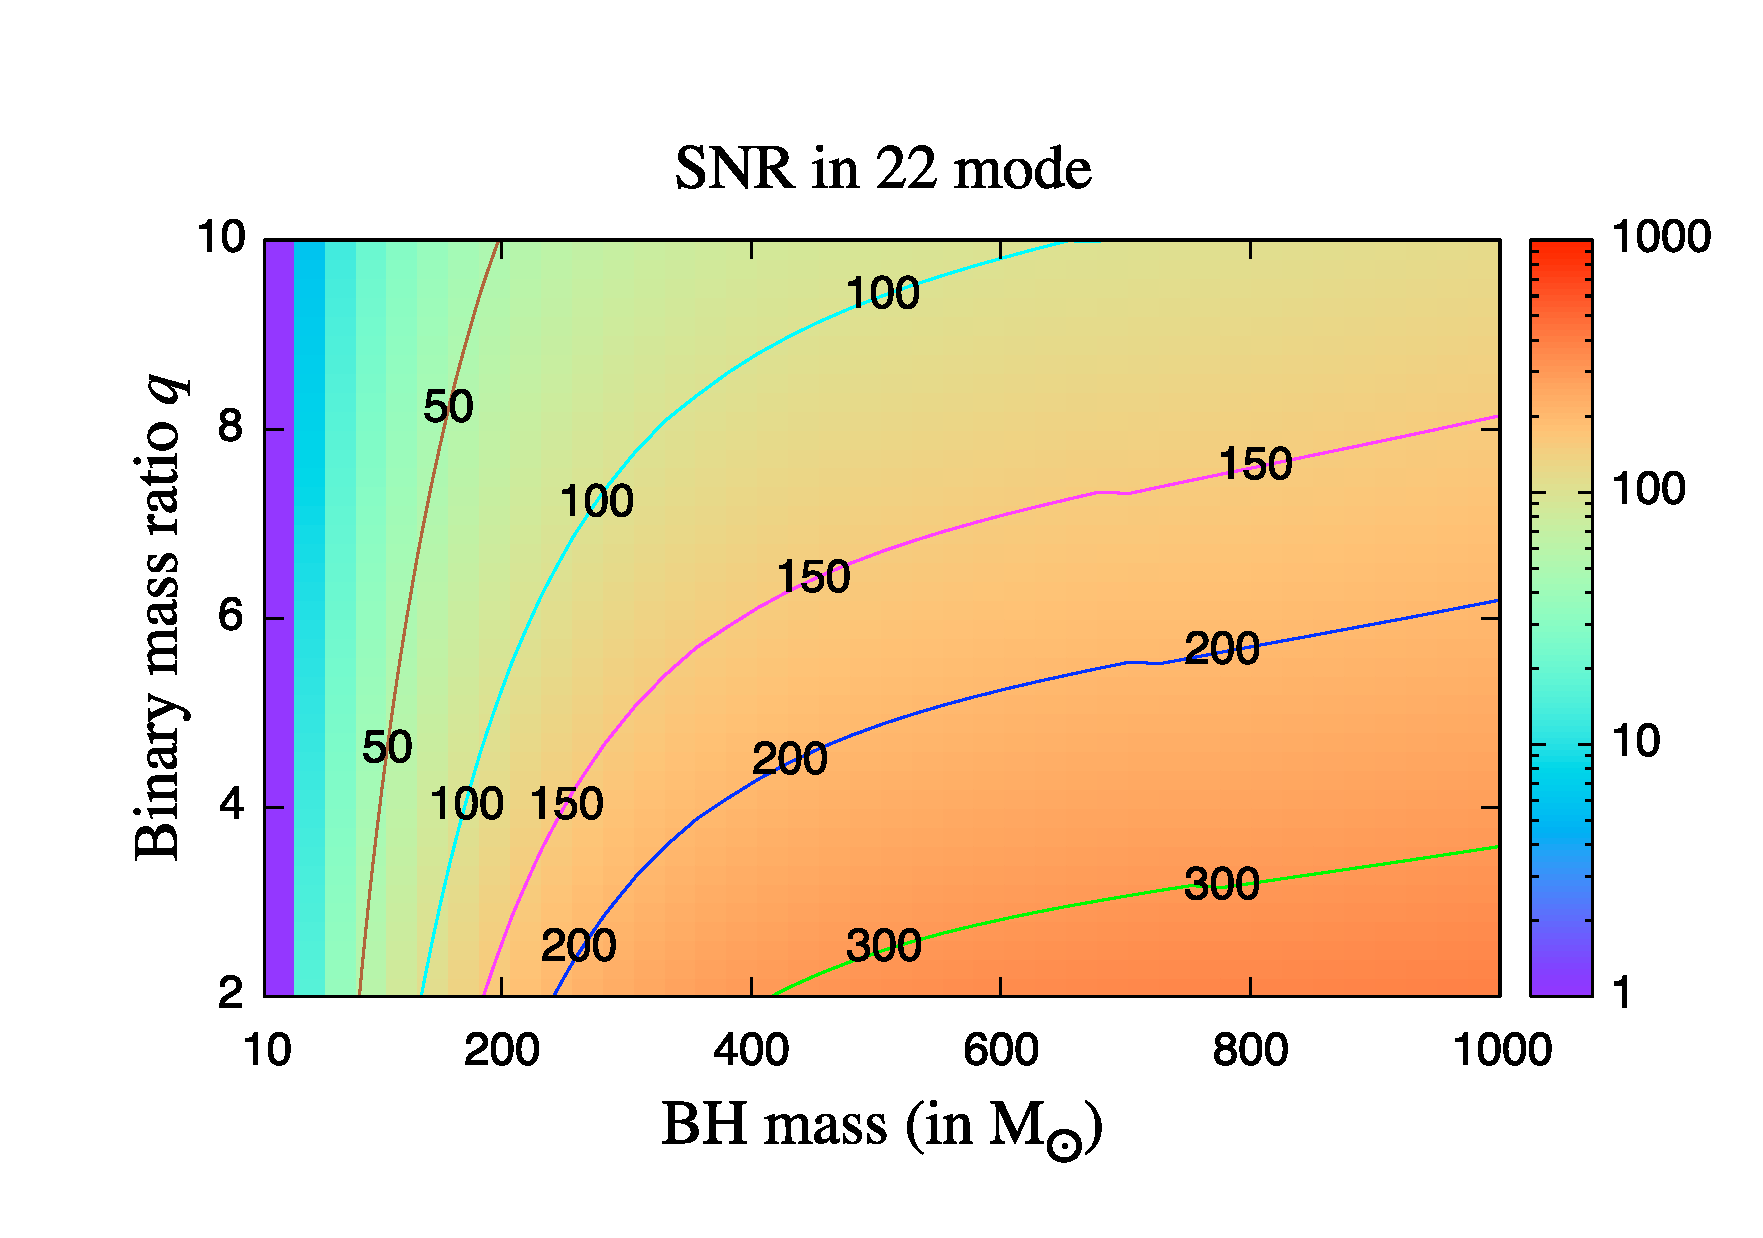
\includegraphics[width=0.45\textwidth]{./Sec_ET_ScienceCase/ET-SNR-22.pdf} \\
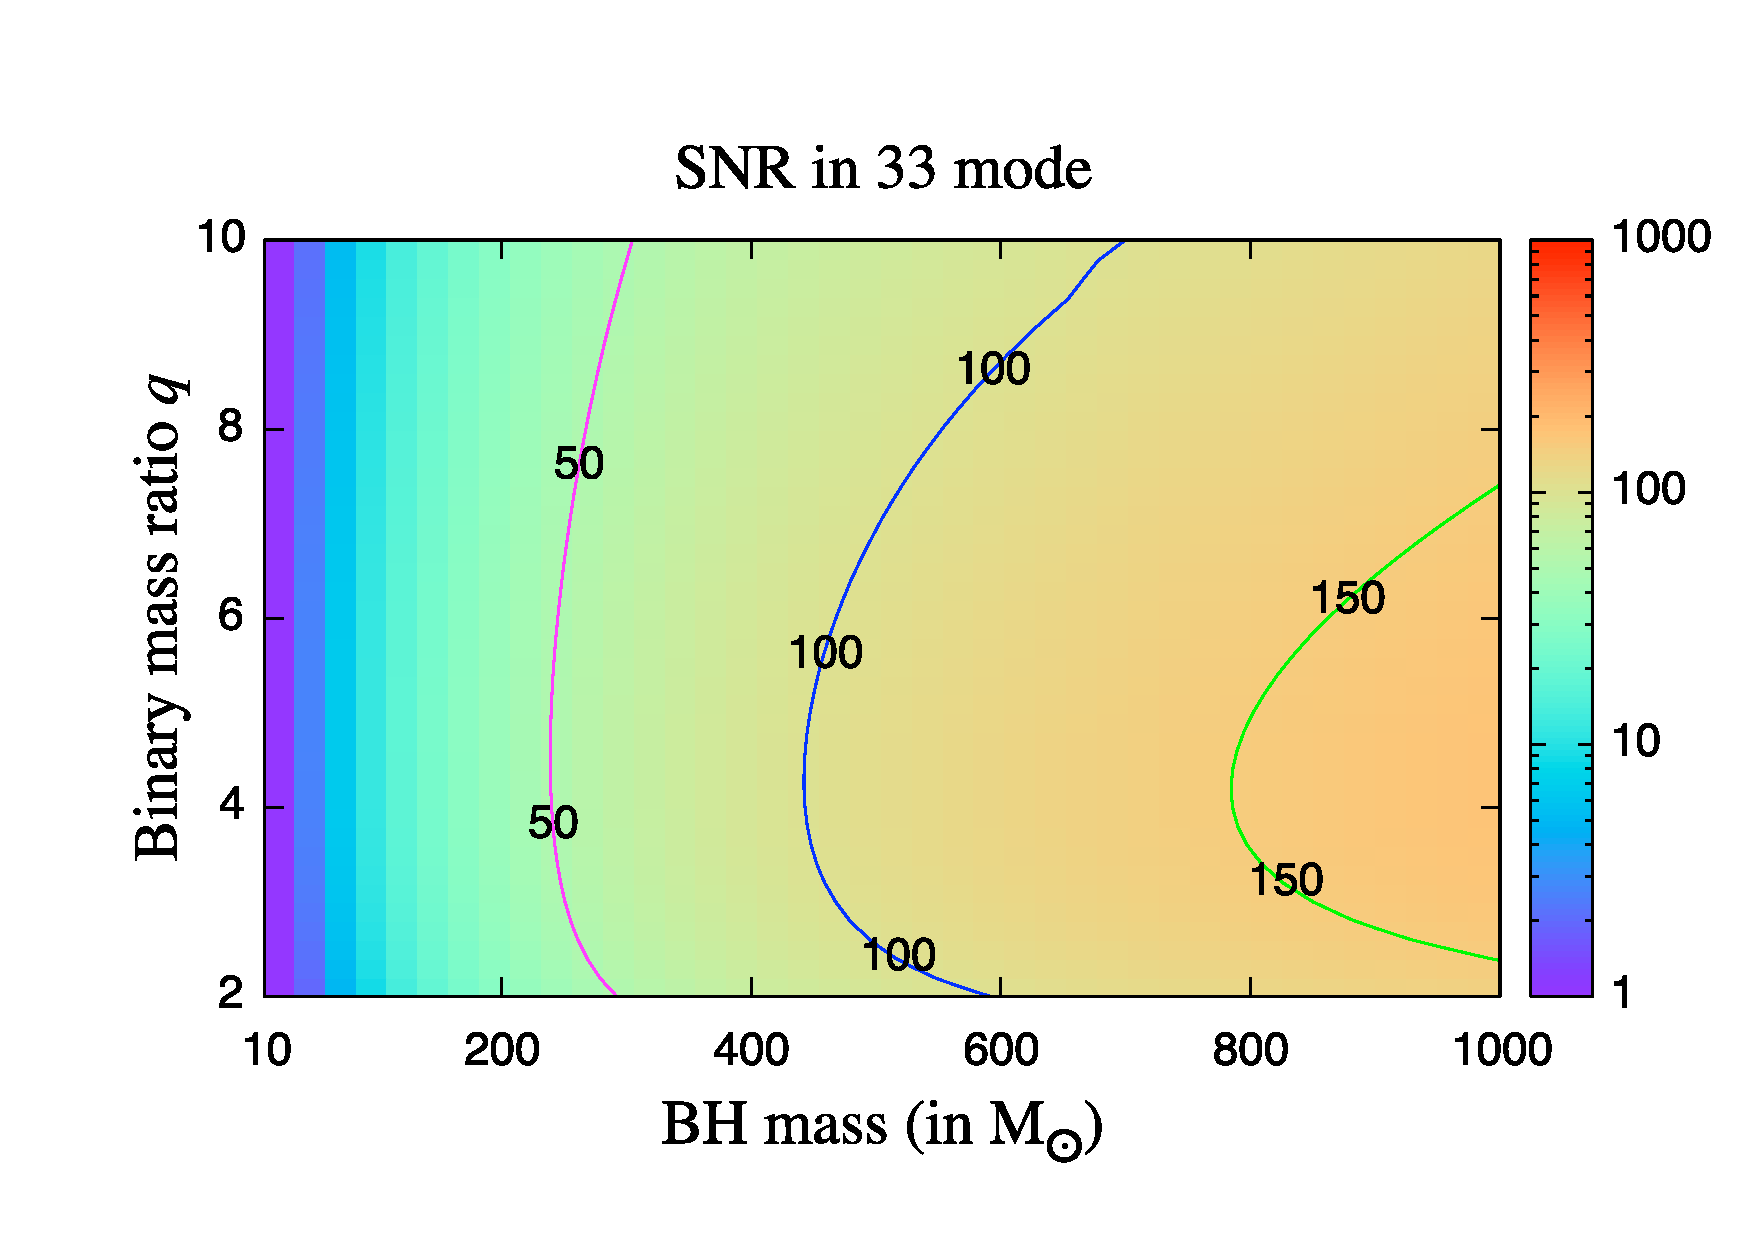
\includegraphics[width=0.45\textwidth]{./Sec_ET_ScienceCase/ET-SNR-33.pdf} &
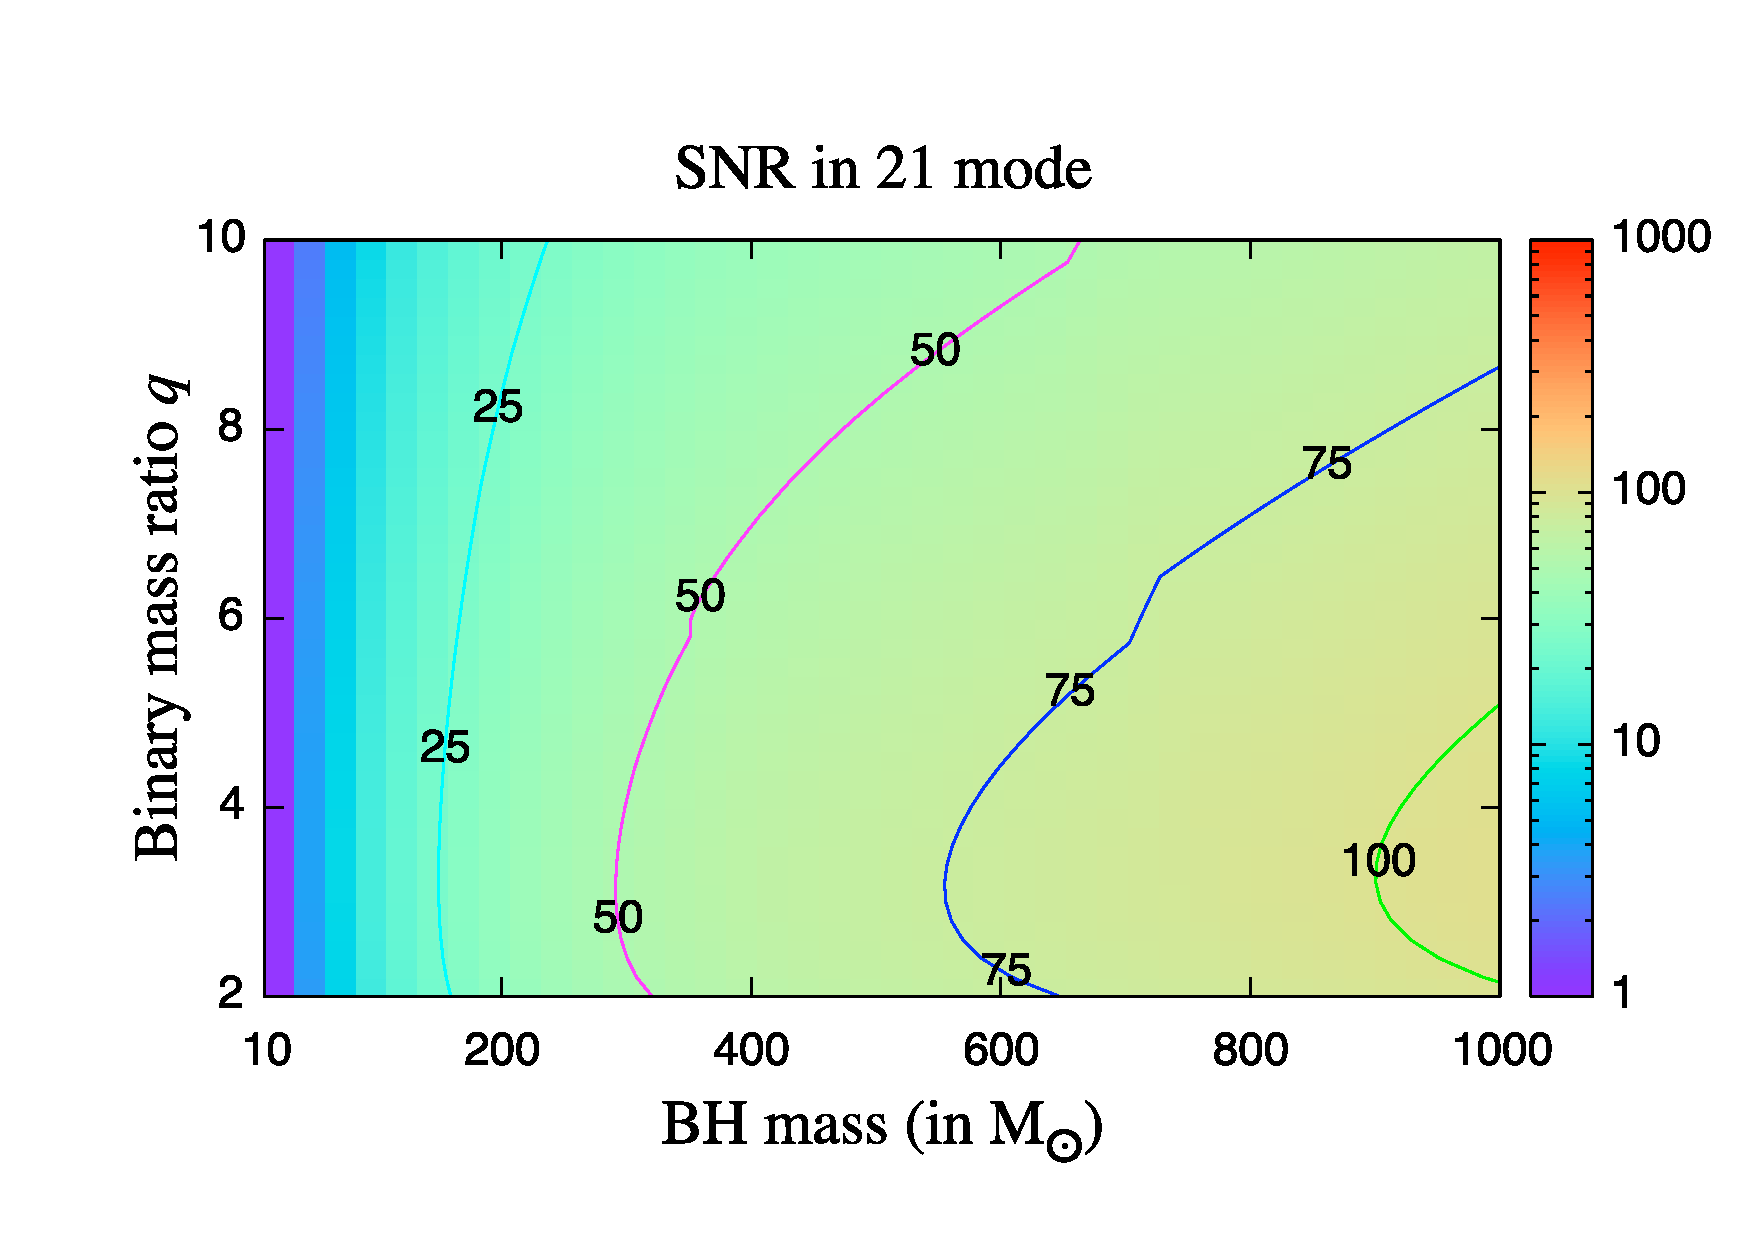
\includegraphics[width=0.45\textwidth]{./Sec_ET_ScienceCase/ET-SNR-21.pdf} \\
\hline
\end{tabular}
\caption{Signal-to-noise ratio of quasi-normal modes in ET as a 
function of the BH's mass $M$ and progenitor binary's 
mass ratio $q$ for different modes. Most of the contribution to the 
SNR comes from the 22 mode but other modes too have significant 
contributions, 33 being more important than 21.} 
\label{fig:snr}
\end{figure}

In BBH systems where one component is much heavier than the other, 
many GW cycles are emitted while the smaller object is in the strong 
field region close to the larger object. These GWs encode a map of 
the spacetime structure in the vicinity of the large BH, which can be 
used to measure properties of the central object~\cite{ryan95}. Using 
such observations to measure spacetime structure has been explored 
extensively in the context of extreme-mass-ratio inspirals (binaries 
of $\sim10M_{\odot}$ objects with $\sim 10^6M_{\odot}$ objects) 
for LISA (see~\cite{AmaroSeoane:2007aw} and references therein). 
There is an analogous source for ground based detectors, namely the 
inspiral of a $\sim1M_{\odot}$ object into a $\sim100M_{\odot}$ BH. 
We refer to these as intermediate-mass-ratio inspirals (IMRIs)~\cite{LIGOimri}.


ET will be able to detect IMRIs out to redshifts $\sim 1$--$5$, 
depending on the mass and spin of the central IMBH \cite{Huerta:2011}. 
Assuming that $\sim10\%$ of globular clusters form IMBHs, ET will detect 
between a few tens and a few hundreds of events, depending on the 
mass distribution of the intermediate mass BHs \cite{Gair:2009ETrev}. The 
biggest uncertainty is in the intrinsic density of IMBHs, which could 
reduce these numbers by several ordrs of magnitude. Advanced LIGO 
observations of IMRIs could be used to make very modest measuements 
of deviations in BH structure from the Kerr metric, e.g., 
an ${\cal O}(1)$ deviation in the quadrupole moment~\cite{LIGOimri,imrirate}. 
ET will observe IMRI events for many more cycles, due to its better 
low-frequency performance, which is very important for the precision of 
spacetime mapping measurements. We would therefore expect to obtain 
constraints that are one or two orders of magnitude better with ET, 
although explicit estimates of this have not yet been made.

\subsubsection{Testing the no-hair theorem using BH quasi-normal modes}
Perturbed Kerr BHs emit gravitational radiation 
which consists of a superposition of damped sinusoids termed 
quasi-normal modes.  The frequencies and time-constants of the modes 
depend only on the mass and spin of the BH --- a consequence 
of the no-hair theorem. It has been proposed that a measurement 
of two or more quasi-normal modes could be used to confirm that the 
source is a BH and to test if GR continues to hold
in ultra-strong gravitational fields.

The fundamental mode frequencies and time constants, characterized 
by two indices $(\ell,m)$, $\ell=2,3,\ldots$ and $m=-\ell,\ldots,\ell,$
are given by the general expressions
\begin{equation}
\omega_{\ell m} = \frac{F_{\ell m}(j)}{M},\quad
\tau_{\ell m} = M G_{\ell m}(j),
\end{equation}
where $F_{\ell m}(j)$ and $G_{\ell m}(j)$ are functions of 
the dimensionless BH spin magnitude, or Kerr parameter, $j$.  
Not all modes are excited equally; when, for instance, two BHs
merge to form a single BH the $(\ell,m)=(2,2)$ mode is the
most dominant followed by $(\ell,m)=(3,3)$ and so on. However,
all mode frequencies and time-constants depend only on the mass 
$M$ and (dimensionless) spin magnitude $j=J/M^2,$ where $J$ is
the magnitude of the BH's spin angular momentum. 
Several authors have noted that this 
aspect of the no-hair theorem could be used to test if massive 
compact objects at galactic cores are actually rotating BHs 
described by the Kerr metric of general relativity 
\cite{BHspect04,BCW05,Berti:2007a}; alternatively, it could be used 
as a strong field test of GR itself \cite{BHspect04}. 

The key idea behind the proposed tests is the following: If one can reliably 
decompose the observed gravitational radiation from a ringing BH into 
a superposition of different modes, then the frequencies and time-constants of 
each of the modes could be used to infer the mass and spin of the BH.
If the object is truly a BH, then the masses and spins obtained
from the different modes should all be consistent within the measurement
errors. Inconsistencies in the values of the masses and spins inferred 
from different modes would be an indication of the failure of GR or that the
radiation was emitted from an object that is not a BH. If a merging
binary does not lead to a BH then the inspiral phase may not
result in a superposition of QNMs that can be characterized by 
just two parameters.  

Figure \ref{fig:snr} plots the SNR in the ringdown
signal (plot titled ``SNR in all modes") and contribution from 
the $(\ell,m)=(2,2), (2,1)$ and (3,3) modes 
as a function of the mass $M$ and mass ratio $q=m_1/m_2$ ($m_1>m_2)$
of the progenitor binary.  Although the (2,2) mode is the most dominant, 
the other modes are large enough that it should be possible to 
disentangle the different modes and test the no-hair theorem.

\paragraph{Testing the no-hair theorem by measuring the multipole 
moments of a source}
There is an alternative way to test the no-hair theorem.
Another consequence of this theorem is 
that the entire spacetime structure, characterised by 
``multipole moments'', is determined by just two parameters, the BH 
mass, $M$, and spin parameter, $S=J/M,$ where $J$ is the magnitude of
the spin angular momentum. It has been demonstrated 
that GW observations can measure the mass and spin multipole moments 
$M_l$ and $S_l$ independently of one another~\cite{ryan95}. We can, 
therefore, directly verify that they satisfy the Kerr relationship
$ M_l + i\,S_l = M(i\,S/M)^l\,. $
We would only need to measure three multipole moments to rule out 
an object as a Kerr BH.

It has been shown that IMRI observations with Advanced LIGO could 
detect an $\mathcal{O}(1)$ deviation in the quadrupole moment of 
an object~\cite{LIGOimri}. The precision achievable with ET should 
be at least a factor of $10$ better than this due to the improved 
low-frequency performance. To put this in perspective, one alternative 
to BHs, boson stars, have quadrupole moments two orders-of-magnitude 
bigger than BHs of the same mass and spin~\cite{ryanBS}.

Any deviations from the no-hair theorem that are detected will have 
profound implications for our understanding of relativity and of BHs. 
Persistent deviations from the theory may lead to important insights 
in the search for a fundamental theory that unifies all four forces 
of nature.
\paragraph{Are there naked singularities?}
% \ledby{Gair}
One of the assumptions of the uniqueness theorem is that a horizon exists in the spacetime. This arises from a belief embodied by the ``Cosmic Censorship Hypothesis''~\cite{CCH} (CCH), which states that any singularity will be enclosed by a horizon. The CCH arises from a desire for predictability in the Universe---when Physics breaks down at a singularity, we do not want information from that to propagate into the rest of the Universe. However, the CCH is unproven and therefore ``naked'' singularities not enclosed within a horizon may still exist. Gravitational wave observations provide a unique way to look for these exotic objects. Observations may be indirect, via detection of a violation to the ``no-hair'' theorem. However, they may also be direct---if a horizon is not present in the spacetime, the gravitational waves will not cut off when the object crosses the horizon~\cite{kesden05}, which will be a clear smoking gun signature for the absence of a clothing horizon in the system.

ET will provide much more stringent constraints on potential violations of the CCH than are possible with Advanced LIGO. ET observations will therefore play an important role in answering the question as to whether naked singularities exist, which could have profound implications for our understanding of various aspects of the theory of relativity.

%\subsubsection{Measuring the mass of neutrinos via supernovae}
%CVDB\\
%\dots

\subsubsection{Limit on the maximum mass of compact stars}

It is generally believed that NSs have masses
between $\sim 1.3\,M_\odot$ and $\sim 2\,M_\odot,$ % [CITATION],
but such statements rely on guesses regarding the EoS of
dense nuclear matter. Above $2\,M_\odot$ a quark star might be created, or
some other exotic object.  Apart from the existence of such objects 
and their properties, an interesting question is how massive
a star can be while still being stable. 

\begin{wrapfigure}{l}{0.5\textwidth}
\vskip -0.3cm
%\begin{figure}
\centering
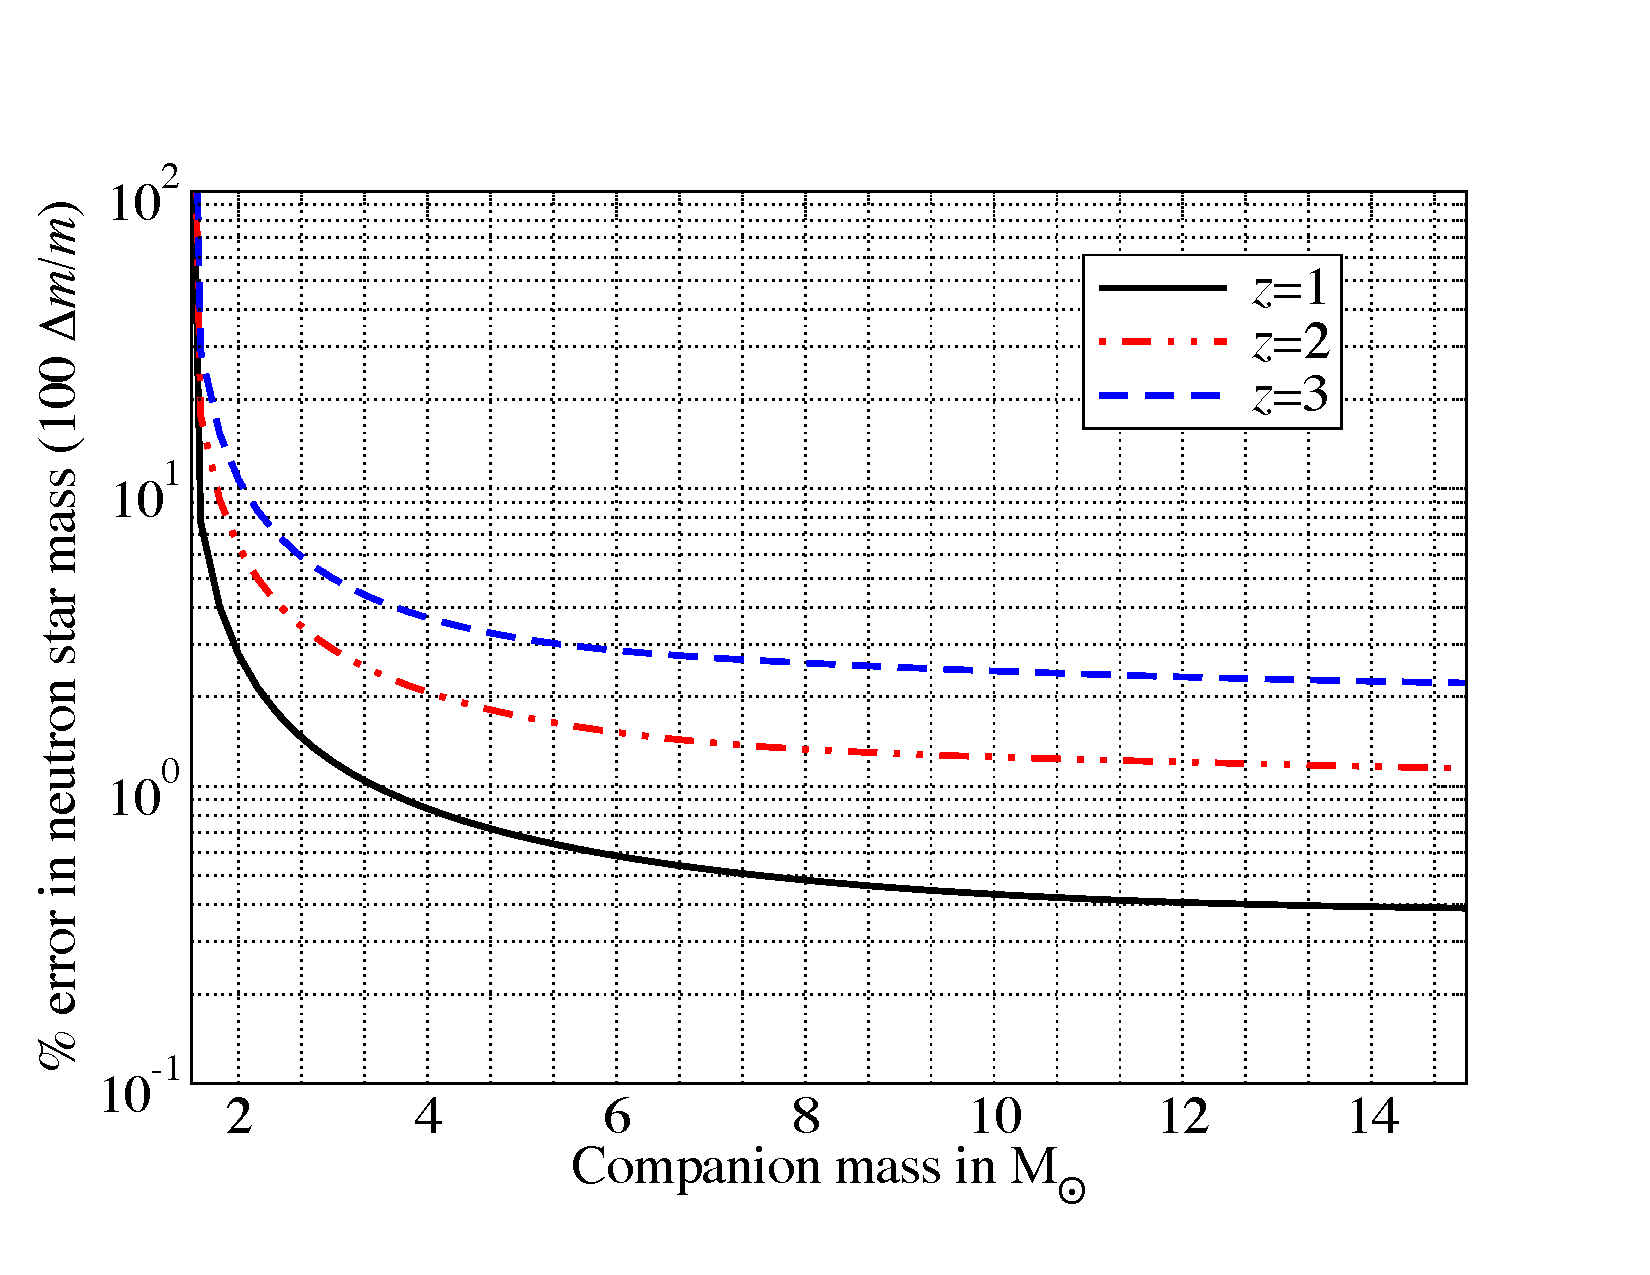
\includegraphics[angle=0,width=0.5\textwidth]{./Sec_ET_ScienceCase/NSmass.pdf}
\caption{The accuracy with which the mass of a neutron star can be 
determined, as a function of the mass of the companion object.}
\label{fig:NS_MassAccuracy}
%\end{figure}
%\vskip 0.9cm
\end{wrapfigure}
Fig.~\ref{fig:ET_range} shows the maximum distance
to which binary inspirals can be seen in ET for systems
with two equal mass companions. The distance reach for a binary
with symmetric mass ratio $\nu$ would be smaller by a 
factor\footnote{A factor of $\sqrt{4\,\nu}$ can be understood in
the following manner: The signal-to-noise ratio of an inspiral
signal is directly proportional to the product of its amplitude 
(which goes as $\nu$) and square-root of its duration (which
goes as $\nu^{-1}$), or an overall factor of $\sqrt{\nu}.$ A
factor of 4 is included for normalization as $\nu=1/4$ for equal
mass systems.} of $\sqrt{4\,\nu}$. For a NS of $2\,M_\odot$ and a
BH of $5\,M_\odot,$ $\nu\sim 0.20$ and so the range would be 
90\% of that for a binary composed of two $3.5\,M_\odot$ system.
Considering NS masses of $1.4\,M_\odot$ and BH masses of $10\,M_\odot$
one gets the distance reach to be $56\%$ of that for a binary
of total mass $16.4\,M_\odot$ and composed of two equal mass
BHs.  The above reasoning shows that ET will have access
to NSBH sources out to genuinely cosmological distances, up to
redshifts of several, with an expected detection rate in the
order of $10^6\,\mbox{yr}^{-1}$. 

Fig.~\ref{fig:NS_MassAccuracy}
shows how accurately ET will measure the mass of a NS 
(assumed to be $1.4\,M_\odot$) in an NSBH
inspiral process, as a function of the mass of the BH for three
different values of the redshift, $z=1,2,3.$ We see that for BH masses 
larger than $2\,M_\odot$ the NS mass is measured to better than
$10\%.$ Indeed, most astronomical BH candidates have a 
minimum mass of $\sim 4\,M_\odot$ and for BH mass $\gtrsim 4\,M_\odot$, 
the NS's mass can be inferred to a fraction of a percent out to
$z=1$, and up to a few percent out to a redshift of 2 or 3. This
would enable us not only to establish the mass distribution of
NSs and possible dense exotic objects, but also the 
evolution of this distribution over cosmological timescales.

\clearpage
\FloatBarrier

\subsection{Astrophysics}
ET will be a unique observatory in many ways to study neutron stars 
and black holes.  It will be sensitive to relativistic phenomena that 
efficiently convert energy in non-axisymmetric motion in compact
objects into gravitational waves. Examples include quakes in neutron 
stars, supernovae, proto-neutron stars, inspiralling and colliding 
binary neutron star and neutron star-black hole systems and gamma-ray 
burst sources, systems and phenomena where motion ought to be 
highly relativistic and hence potential sources of GW too.
In this Section we will look at what ET can unveil about compact 
objects and their environs.

\subsubsection{Determining the neutron star equation of state from 
binary coalescences}

% \ledby{Rezzolla, Read}
% \textcolor{blue}{Probing the ground-state of nuclear state over a
% range of nuclear density, measuring the effects of neutron star
% equation of state using binary neutron star mergers, and measuring
% magnetic fields, post-merger oscillations}

Several BNS systems have been observed to date, for some of which
general-relativistic effects in the binary orbit have been measured 
to high precision \cite{Living:Lorimer}. The inspiral and merger of 
two NSs in binary orbit is the inevitable fate of close-binary
evolution, whose main dissipation mechanism is the emission of
GWs.  The detection of GWs from
NS binaries will provide a wide variety of physical
information on the component stars, including their mass, spin, radius
and EoS.  The central densities of isolated
NSs, in fact, can range up to ten times the nuclear saturation
density, and during the merger and coalescence of two NSs
the maximum density will rise even further, before the remnant object
collapses to a BH.  The behaviour of bulk matter at these
densities is not well understood; measurements of GW
signals from NS sources can usefully constrain the
EoS at these densities.

Quantum chromodynamics is expected to be a complete description of matter
at these energies; the uncertainty in theoretical understanding comes from
the many-body problem with strong interactions. The description of bulk
neutral matter in terms of hadrons such as protons and neutrons may need to
be expanded to accomodate new particles that are formed at these energies,
such as hyperons, pions, and kaons. In fact the appropriate degrees of
freedom describing cold matter at very high density may no longer be
hadrons but the quarks and gluons themselves, in some form of quark matter.

While isolated or inspiralling NSs are well described by the
ground state of matter, i.e.\  with a ``cold'' EoS, the
temperatures reached in the coalescence as a result of the strong
shocks will be significant and of the order of $\sim 10^{10}$--$10^{12}$\,K. 
Yet, just as measurements of the hot out-of-equilibrium ion
collisions in the Relativistic Heavy Ion Collider 
constrain the ground state of dense nuclear matter,
observed characteristics of NS mergers may be able to
constrain the ground state of dense neutral matter.
Reviews of the current range of candidate equations of state, 
and constraints on them from astrophysical observations and 
heavy ion collision experiments, can be found in 
\cite{LattimerPrakash2007,Klahn2006,PageReddy2006}.

The signature of the NS EoS can be found in almost any
NS sourced GW: in the peak frequencies of
supernova waveforms \cite{Dimmelmeier2007,Marek2008}, in the
possibility of accretion-induced crust mountains \cite{Owen05,
Watts2008}, and in the astroseismology of glitches and other
oscillation mode excitations.  Studies which have specifically
explored the effect of varying EoS (or varying compactness for a given
mass, which implies variation of EoS) on GW spectra
include Refs.\,\cite{ZhugeEt1996, RasioShapiro1999, FlanaganHinderer2007,
Read:2008pp, Read:2009bns} for binary NS inspiral,
Refs.\,\cite{Bejger05,Shibata05c,Shibata2005eos, Oechslin06,Oechslin07b,
Yamamoto2008,Baiotti08,Baiotti:2009gk} for binary NS
coalescence, and Refs.\,\cite{Faber05,LattimerPrakash2007,
ShibataTaniguchi2008,Shibata:2009cn} for mixed
NSBH binaries.  

\begin{figure}
\begin{center}
%\hskip -0.2cm
%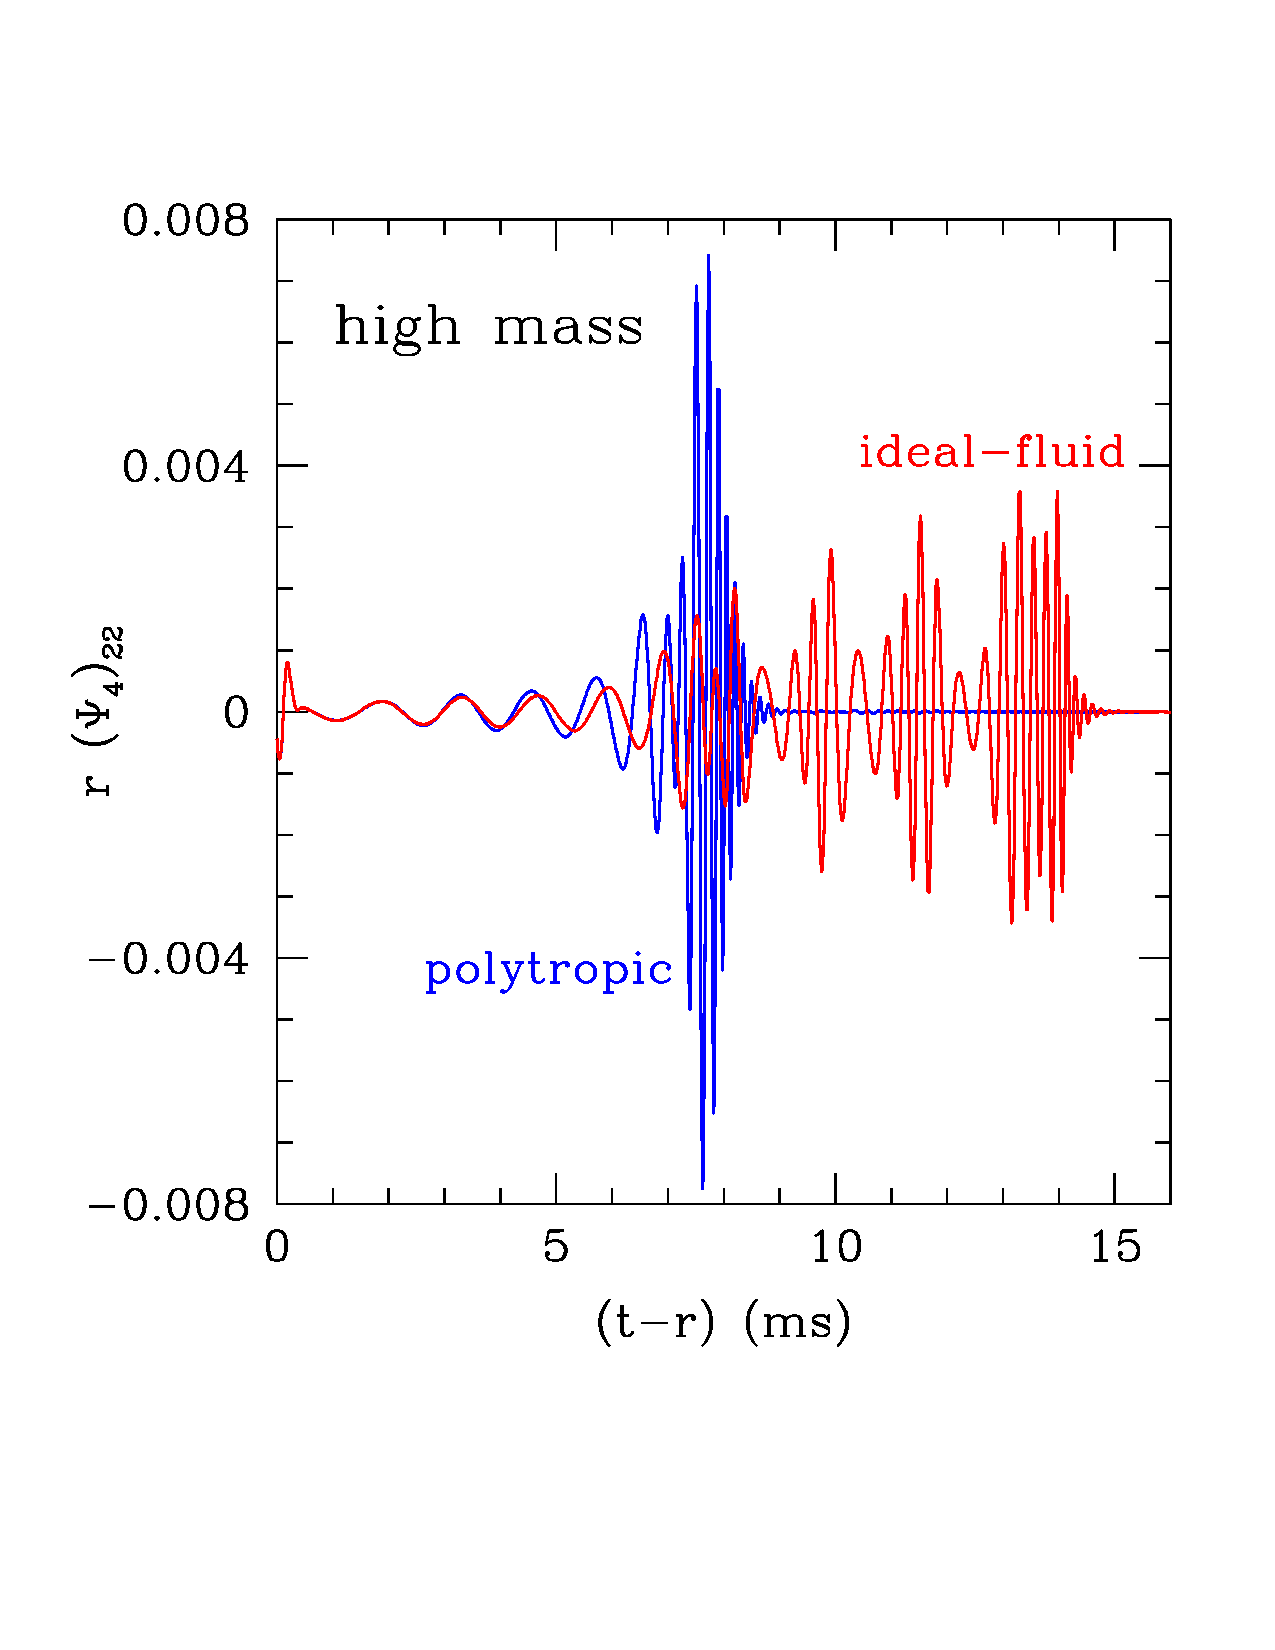
\includegraphics[angle=0,width=0.49\columnwidth]{./Sec_ET_ScienceCase/Psi4_pol_vs_IF_high.pdf}
%\hskip -0.5cm
%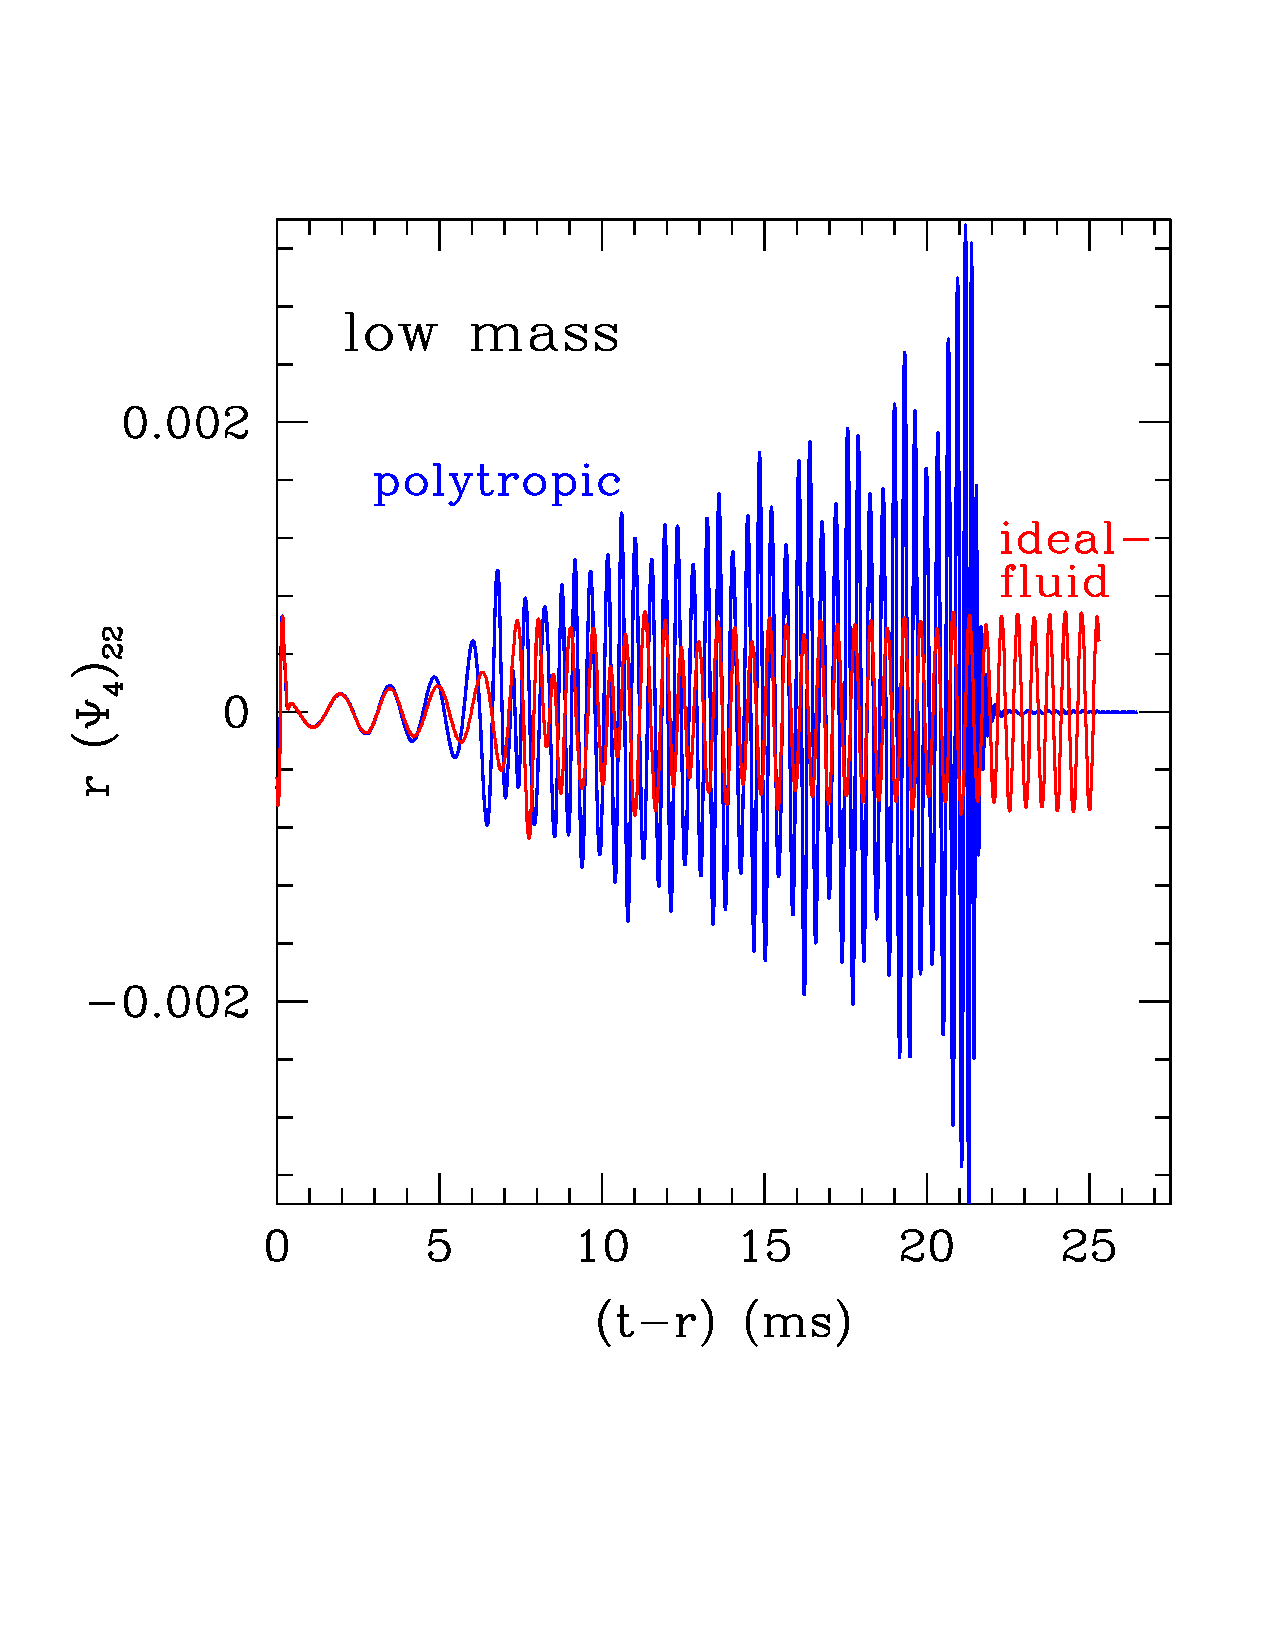
\includegraphics[angle=0,width=0.49\columnwidth]{./Sec_ET_ScienceCase/Psi4_pol_vs_IF_low.pdf}
%\vskip -1.2cm
%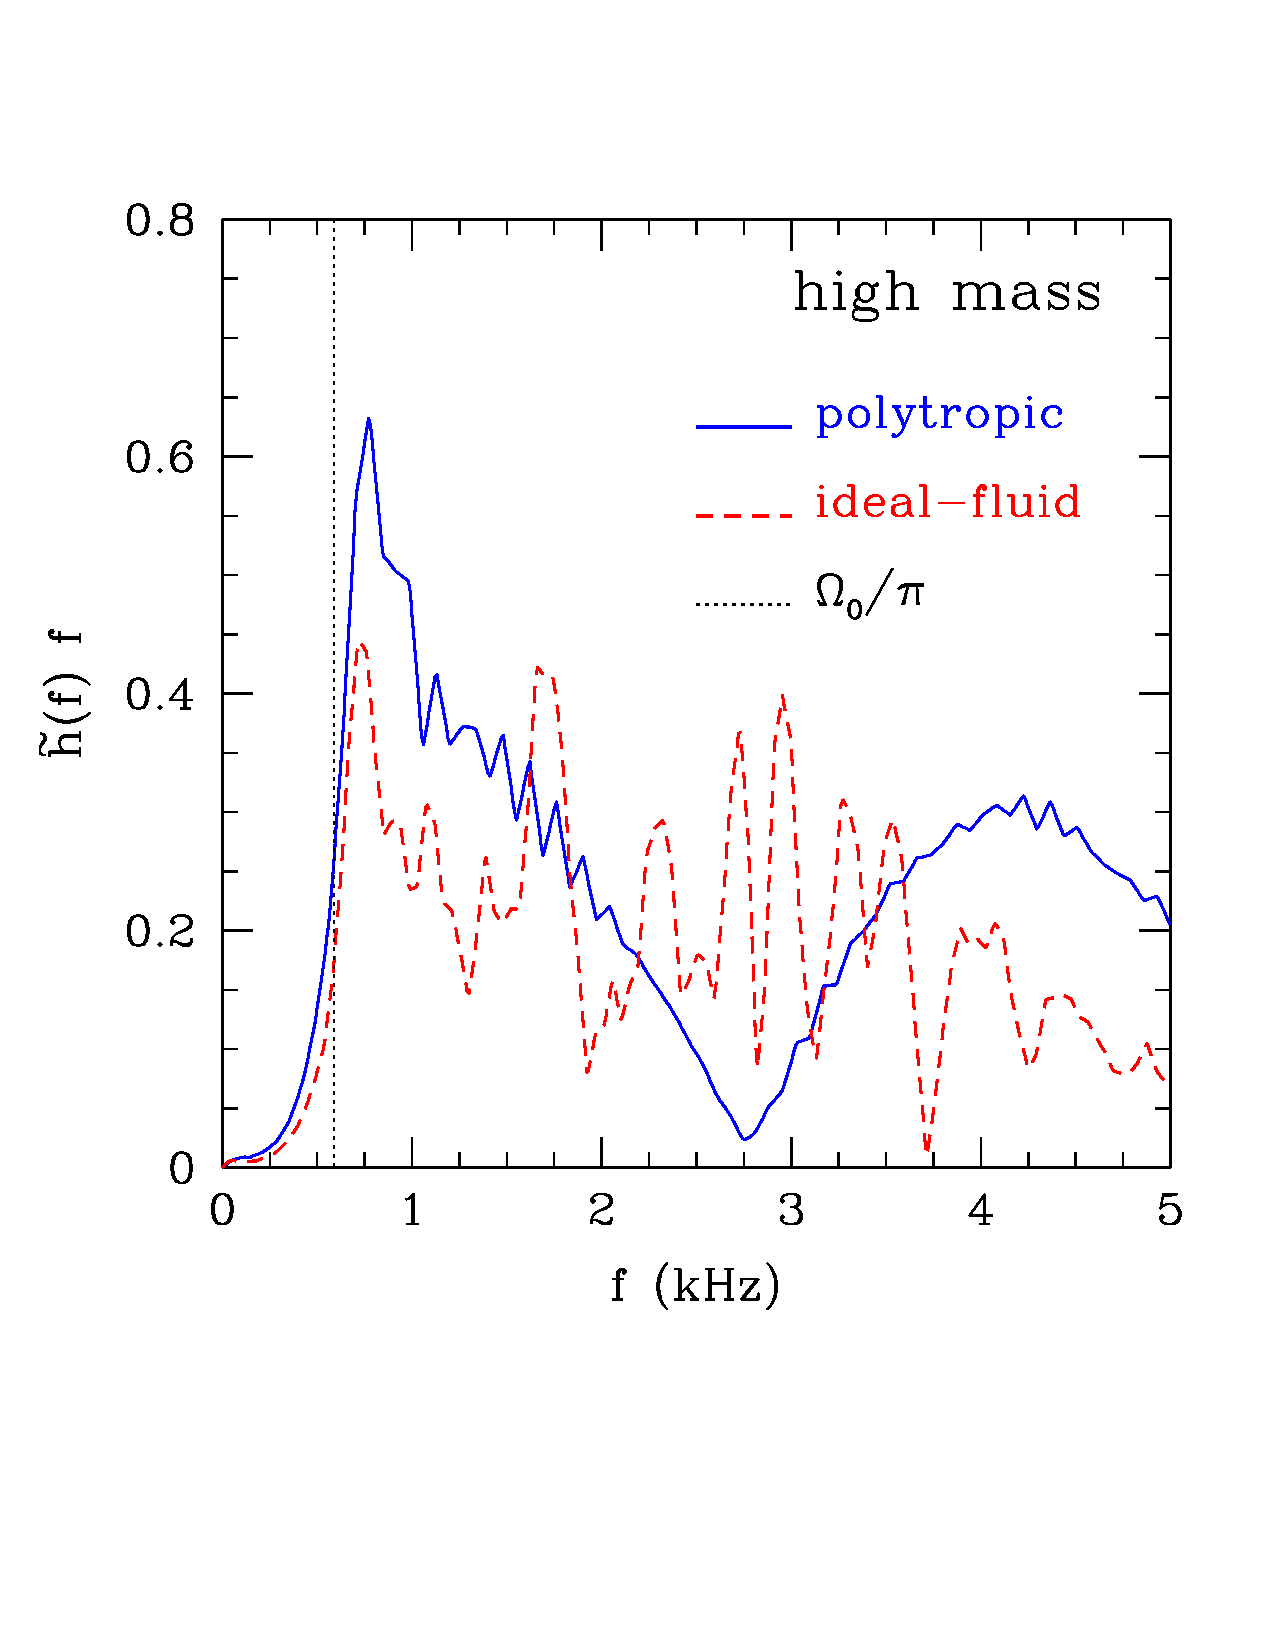
\includegraphics[angle=-0,width=0.45\textwidth]{./Sec_ET_ScienceCase/PSD_h_pol_vs_IF_high.pdf}
%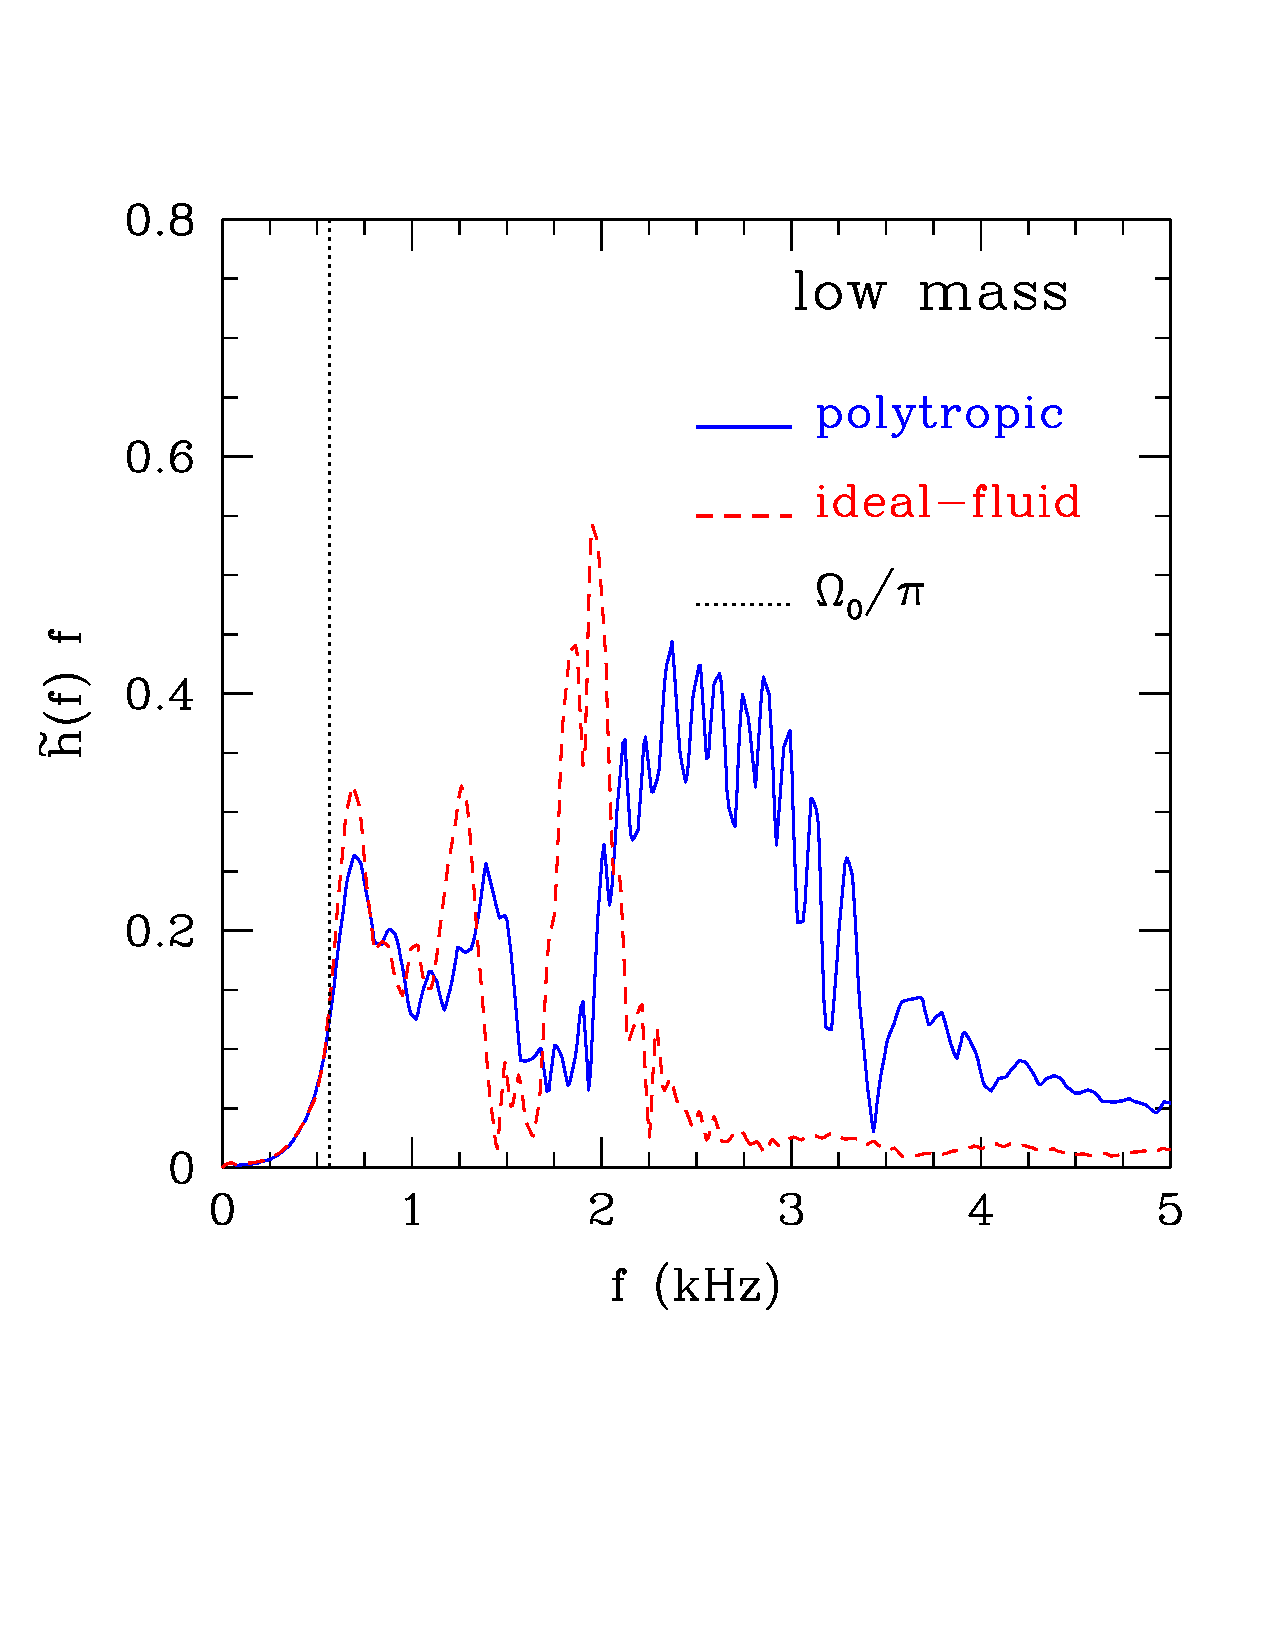
\includegraphics[angle=-0,width=0.45\textwidth]{./Sec_ET_ScienceCase/PSD_h_pol_vs_IF_low.pdf}
\includegraphics[angle=-0,width=0.45\textwidth]{./Sec_ET_ScienceCase/highmass-NS.pdf}
\hskip 0.2cm
\includegraphics[angle=-0,width=0.45\textwidth]{./Sec_ET_ScienceCase/lowmass-NS.pdf}
\caption{
Gravitational wave spectra of merging neutron star binaries compared to
sensitivities of Virgo, advanced LIGO (labelled adLIGO) and ET. 
Left panel shows spectra of high-mass binaries evolved with the cold 
(blue solid line) or hot (red dashed line) equations of state. Also
shown for comparison is the corresponding spectrum of an equal-mass, 
non-spinning binary black hole with total mass $M=200\,M_\odot,$
which appears in the low-frequency part of the spectrum (orange solid 
line). Right panel is the same as the left panel but for the 
low-mass binary.  It can be seen that the observed spectra are 
sensitive to the neutron star EoS.
%\textit{Top row, left panel:} Comparison of the waveform 
%for a high-mass NS binary (with a total mass of
%$3.2\,M_{\odot}$) when evolved with the a ``cold'' EoS (labeled
%as `polytropic') or with a ``hot'' EoS (labeled `ideal-fluid').
%\textit{Top row, right panel:} The same as in the left
%panel but for a low-mass NS binary (total mass 
%$2.9\,M_{\odot}$). \textit{Bottom row:} The same as in the top
%row but with the comparison being made in frequency
%space with the sensitivity curves of Virgo, advanced LIGO and Virgo
%and ET-B. The source is assumed to be at 300 Mpc.
\label{NS_example}}
\end{center}
\end{figure}

Gravitational waves from binary inspiral and merger are
expected to be frequently observed in ET and the predicted signals have
several interesting EoS-dependent features.
This is illustrated in Fig.\,\ref{NS_example}, based on the simulations
of~\cite{Baiotti08} where a comparison of GW spectra from
BNS mergers is shown together with the noise PSDs of 
Virgo, aLIGO and ET. The panel on the left plots the spectra for 
a system with total mass $2.98\,M_\odot$ while the one on
the right considers a lighter system of total mass $2.69\,M_\odot.$
Both panels show spectra for two different EoS: NSs with the cold EoS 
give rise to two distinct bumps (blue solid lines), the location
and relative heights depending on NS masses. NSs with
the hot EoS exhibit a number of spikes (red dashed lines)
whose detailed structure depends on the NS masses.  
The spectrum of a BBH merger (orange solid lines), on the other 
hand, has no specific feature and is independent of the total
mass of the binary.  While neither of the two equations of state 
considered here are realistic, they span in some sense the extremes 
of the range of possibilities.  Most importantly they show that the 
GW signal from BNS merger will be very sensitive to the mass of 
the stars and their EoS.

While this is especially true in the post-merger phase, the
inspiral phase will also provide important information on the EoS. 
Although for most of the inspiral phase, the component stars of 
a BNS system are well-modeled as point particles, as they approach 
each other, an EoS-dependent tidal deformation modifies their orbits,
changing the late inspiral waveform. The measurability of this effect
in GW detectors can be estimated using both
PN tidal deformation calculations and full numerical
simulations of BNSs with varying EoS. The induced change in the
waveform can be used to measure the radius of the NS quite accurately.

Indeed, the set of numerical simulations of Ref.\,\cite{Read:2009bns} 
show that for a $1.35\, M_{\odot}$--$1.35\, M_{\odot}$
system at $100$\,Mpc ET can measure the radius to within
$\pm 0.5$--$1.0$\,km.  This compares favorably to the range in
predicted radius of roughly 9--16 km.  Parameterizing the variation in
the size of a NS by the pressure at a density of $5\times10^{14}$\,g\,cm$^{-3}$
\cite{Read:2008pp}, gives fractional uncertainty in pressure of 5--10\%.  

%Tidal deformation in NSs is characterized by the parameter 
%$\tilde{\lambda}(m_1,m_2)$ which ranges between $0.5 \times 
%10^{36}$\,g$^2$\,cm$^2$ and $10 \times 10^{36}$\,g$^2$\,cm$^2$ 
%for realistic EoS.  Flanagan and Hinderer 
%\cite{FlanaganHinderer2007} estimate that for a binary at 50\,Mpc
%\begin{itemize}
%\item $\Delta \tilde{\lambda} \sim 1.22 \times 10^{36}$ for $1.35-1.35
%M_\odot$
%\item $\Delta \tilde{\lambda} \sim 1.6 \times 10^{36}$ for $1.45-1.45
%M_\odot$
%\item $\Delta \tilde{\lambda} \sim 1.85 \times 10^{36}$ for $1.35-1.7
%M_\odot$
%\end{itemize}
%for the inspiral phase \emph{below 400\,Hz}. 

The advantage of ET in understanding the NS EoS is not
necessarily the larger number of detections possible with increased
sensitivity, although information about the mass distribution of NS 
populations can also be useful for constrainting the EoS. Instead, ET
will provide very strong signals at reasonable rates; for example two
$1.4\,M_\odot$ NSs inspiralling towards each other within an
effective distance of 100\,Mpc, which is expected roughly once a year,
would give a SNR in ET of over 900.  This makes it possible to precisely
measure the component masses during the early inspiral phase, to detect
small departures from point particle behaviour at moderate
frequencies, and discriminate between merger and post-merger signals
from different models at high frequencies.

An interesting feature that has emerged from studies of BNS
coalescences is the post-merger formation, in some cases, of a
hyper-massive remnant object which oscillates and emits GWs
on fairly long timescales.  The presence or absence of such
post merger oscillations, as well as their characteristic frequency
and duration, varies with the cold EoS. However, they are additionally
sensitive to many physical characteristics such as thermal properties, 
magnetic fields, particle production, and so forth.  The precise details of
the signal are not easy to predict.  However, the signal from such 
a post-merger oscillation should be visible in ET \cite{Shibata2005eos}, 
and analysis of the signal following a measured inspiral phase may provide
useful constraints on the underlying astrophysics.

%It has recently become possible to compute the first complete and
%accurate simulations of the merger of a NS binary through
%to the delayed formation of a BH and its ringdown~\cite{Baiotti08,
%Baiotti:2009gk}. By computing the complete GW signal produced in 
%the process it was possible to show that the emitted signals
%are strongly correlated to the properties of the sources
%emitting them. Differences in the EoS or in the initial mass of the
%system produced different signals with different power spectra and
%different durations.

Furthermore, magnetic fields are commonly present in 
NSs and their possible impact on the dynamics of BNSs
has only begun to be examined.  The effect of magnetic fields on GW
emission during the inspiral and merger of magnetized NSs has 
recently been investigated~\cite{Giacomazzo:2009mp}. It
has been shown that while initial fields of strength 
$B_{0}\gtrsim 10^{12}\,{\rm G}$ have an impact after the merger,
fields of sufficiently strong strength $B_{0}\gtrsim 10^{16}\,{\rm G}$
will affect the inspiral phase too.
%These results are quantified by computing the
%overlap between the waveforms produced during the inspiral by
%magnetized and unmagnetized binaries. 
ET provides a strong impetus for such theoretical studies.  By 
including more realistic equations of state and realistic radiation 
transport schemes, it will be possible to considerably increase our 
level of understanding of these objects. 

\FloatBarrier
\subsubsection{Neutron star physics from pulsar glitches}

% \ledby{Glampedakis}
Many radio pulsars exhibit {\em glitches,} events in which 
a NS is seen to suddenly spin-up, followed by a relaxation period towards
stable secular spin-down. Pulsar glitches have a long observational 
history (beginning shortly after the discovery of the first pulsar)
\cite{Anderson:1975}. 
So far, over a hundred pulsars are known to have glitched at least once
(for a recent survey, see, Ref.\,\cite{Espinoza:2011pq}).
Glitches have also been observed in magnetars --- highly magnetized NSs.
The archetypal glitching pulsar is Vela, which exhibits regular
large glitches with an amplitude corresponding to a fractional spin 
frequency change of the order of $10^{-6}$\,\cite{Ruderman:1976}.

Despite the wealth of observational data, the glitch
remains an enigma from a theoretical point of view \cite{McDonald:2007}. 
It is widely 
believed that glitches are related to the existence of superfluids 
in the interior of mature NSs and that they involve a transfer 
of angular momentum from a superfluid component to the rest of the 
star which includes the crust (to which the pulsar mechanism is presumed 
to be rigidly attached) and the charged matter in the 
core \cite{Anderson:1975, McDonald:2007}.  Key to this idea is the fact that 
a superfluid rotates by forming an array of quantized vortices. 
In essence, the superfluid can spin down only if
the vortices can move outwards.  If the vortex motion 
is impeded by `pinning' to the other component, e.g. the crust nuclei, 
then the superfluid 
cannot keep up with the spin-down due to electromagnetic braking. 
As a result a rotational lag develops between the two components,
until some critical level is reached at which the vortices unpin and 
transfer angular momentum to the rest of the star, and the two 
components are driven to corotation.

Taking the basic two-component picture at face value,  one can estimate 
the available energy that may be radiated at a glitch event. This 
suggests that large Vela glitches may release an energy of the order 
of  $ 10^{42}$~erg ($10^{-12}\,M_\odot$). This is a useful estimate 
as it provides an idea of how energetic regular neutron star events in 
our galaxy may be.  Of course, one must keep in mind that this 
energy may not be associated with GW emission at all. This depends 
on the detailed glitch mechanism, e.g. the asymmetries involved. 
From a general point of view, on would expect glitches originating 
in the star's crust to be associated with very weak GWs (the involved 
densities are simply too low to be relevant). As the standard glitch 
scenario is associated with vortex pinning to crust nuclei, this 
would rule out these events are interesting GW sources. However, 
there is some evidence that the largest observed glitches may require 
the fluid core to be involved (e.g. through pinning of vortices to 
superconducting fluxtubes). This may change the situation dramatically, 
as the denser regions of the star are now involved. It also hints at 
the interesting possibility that the observed phenomenon could be the 
``tip of the iceberg'', reflecting more energetic dynamics in the 
fluid core. This is, of course, speculative but it is relevant to 
note that the level of sensitive of ET may set strong upper limits 
on the possible scenarios. Translating the rough energy estimate into 
a GW amplitude, by assuming that the energy is released through the 
f-mode (a frequency of 2~kHz lasting for a fraction of a ms at a 
distance of 10~kpc) we find an effective amplitude around 
$10^{-23}$. (This estimate assumes we can do matched filtering, which 
is relatively easy for these damped sinusoids.) A signal of this 
strength should be within the reach of ET.  An observed signal  
would immediately constrain the cold-matter nuclear 
EoS\,\cite{AnderssonKokkotas1998, Living:AnderssonComer}. A lack of 
detection would set relevant limits on the asymmetry and fluid 
dynamics associated with pulsar glitches.  
%[CHECK MELATOS]

In order to do better than these rough estimates we need to improve 
our understanding of superfluid hydrodynamics and possible 
instabilities leading to glitches.  There has been some recent 
progress on this, and it seems reasonable to expect the theory to 
have developed significantly by the time of ET construction. There 
has been particular progress on the issue of the origin of the 
glitches, e.g. the instability that triggers large-scale vortex 
unpinning. A recent model suggests that the glitch trigger-mechanism 
may be the result of a superfluid  ``two-stream'' instability 
setting in through the inertial modes of the system 
\cite{Andersson:2002dv,Andersson:2002zd}. However, in this model 
the unstable modes have very short wavelengths and would not be 
effective GW emitters. Whether the idea can be developed into a 
more complete scenario remains to be seen.

Regardless of the theory uncertainties, an instrument like ET would 
be ideal for detecting a GW signal in the 10--100\,Hz band, which 
would be the relevant for the inertial modes of a Vela-like pulsar. 
The detection of GW signals from glitching pulsars would provide a 
tool for probing the interior matter of NSs and supplement EM 
observations.  The realisation of this exciting prospect will require 
(as in the case of other potential sources of gravitational radiation) 
the input of theoretical waveform templates. These waveforms need to 
be computed using detailed multifluid hydrodynamical models for 
superfluid NSs, accounting for effects like vortex mutual friction 
and pinning.

\FloatBarrier
\subsubsection{GW from the r-mode instability}

% \ledby{Leone B. Bosi}

Neutron stars may suffer a number of instabilities. These instabilities 
come in different flavours, but they can all be directly associated 
with unstable modes of oscillation \cite{Andersson:2003}.
A study of the stability properties of a relativistic star is thus 
closely related to an investigation of the star's various pulsation 
modes.  Furthermore, non-axisymmetric stellar oscillations will 
inevitably lead to the production of gravitational radiation.  
Detection of these signals would allows us to  put constraints on 
the interior structure of the star and the extreme physics associated 
with the high-density region.

The most promising instability scenarios concerns rotating stars.  
Of particular interest are the GW driven instabilities of the 
f-modes and the r-modes.  The action of the former is to deform 
the star into a bar-shape, which is an ideal GW emitter.  Meanwhile, 
the r-mode radiate predominantly through the current multipoles. 
The radiation mechanisms are rather different, but the issues 
involved in studying these instabilities are very much the same.  
First we need to establish that the modes can become unstable in 
a realistic neutron star.  This means that the GW driven growth 
must overcome the relevant dissipative damping mechanisms.  We 
need to consider the (standard) shear- and bulk viscosities, and 
understand how the associated rates depend ion the star's 
composition. We also need to consider more exotic mechanisms, e.g. 
strong bulk viscosity associated with hyperon reaction and vortex 
mediated friction in a superfluid mixture. Significant effort has 
gone into these problems in the last decades.  The current 
understanding is that the instability of the r-modes is likely to 
be the most relevant, but scenarios associated with the  unstable 
f-modes should definitely not be ruled out. Basically, the threshold 
for the r-mode instability to set in in a mature neutron star is 
a relatively low fraction of the break-up rotation rate. Meanwhile, 
the f-mode become unstable only near the break-up limit.  Moreover, 
the f-mode instability is thought to be completely suppressed in a 
superfluid neutron star (due to the vortex mutual friction).  This 
is not the case for the r-modes, which are not dominated by this 
mechanism. 

However, detailed modelling suggests that the r-modes reach nonlinear 
saturation at relatively low amplitudes. This limits the GW emission. 
The underlying mechanism, the coupling of the r-mode to a large 
number of short wavelength inertial modes, also leads to the GW 
signal being immensely complex (leading to difficulties to carry 
out matched filtering). Having said that, the best current estimates 
suggest that the r-mode signals should be detectable from systems 
in our galaxy (and slightly beyond) \cite{Bondarescu:2009}.  The 
detectability of the f-modes may be more favourable. In particular, 
recent work shows that the growth time of the f-mode instability 
may be extremely short. However, it is not known if the f-mode 
instability saturates at low amplitudes. If it does not, then the 
associated signals may be detectable from the Virgo cluster. This 
would increase the event rate which would counter the fact that 
we need a very fast spinning neutron star at birth for the mechanism 
to operate.  Further theory progress is needed to make more precise 
statements. What is undoubtedly clear is that, if these GW signals 
are at a level that would be detectable by second generation 
detectors (as suggested) then ET will provide a supreme instrument 
for extracting the relevant physics information. This is a 
tremendously exciting prospect, given the dependence on interior 
neutron star physics that is very difficult to probe by other means.

\paragraph{The strength of gravitational waves from r-modes}
In order to estimate the GW signal associated with the unstable 
r-modes, let us make use of a simple phenomenological model. 
The model accounts for the differential rotation induced by 
the modes~\cite{SaTome}, but does not account for much of the 
complicated core physics considered in other work.  Nevertheless, 
the estimates provide a useful guide to the relevance of these 
GW signals.  Thus detection of such GWs is more difficult than 
initially supposed. In the model, the amount of differential 
rotation is described by a parameter $K$, which encodes the 
level of differential rotation and which may take values in 
the range $[-5/4, 10^{13}]$ depending on the initial conditions.

The detectability of GW produced by r-modes depends upon the 
amount of angular momentum that they carry away. As described 
in \cite{SaTome1}, for $K=0$, the total angular momentum of 
the star decreases to $65\%$ of its initial value, and 
part of the initial angular momentum of the star, about $58\%$, 
is transferred to the r-mode as a consequence of the rapid 
increase of the average differential rotation. Therefore the 
initial angular momentum carried away by gravitational waves 
is about $35\%$. This result is strongly dependent on the value 
of $K$: for higher $K$ the amount of angular momentum carried 
away by gravitational waves may even fall below $1\%$.

\begin{wrapfigure}{l}{0.5\textwidth}
\includegraphics[width=0.5\textwidth]{./Sec_ET_ScienceCase/Rmodes_redone.pdf}
\caption{Detectability of r-modes expected in 
Einstein Telescope (ET-B sensitivity) as a function of the $K$ parameter
describing the strength of differential rotation.}
\label{fig:RmodesVsET}
\end{wrapfigure}
%
In the case of the r-modes, the frequency $f$ of the GWs
depends on the NS's angular velocity $\Omega$ as $f=2\Omega/(3\pi)$. 
The frequency range is estimated as follows:
$f_{min} \simeq [77-80]\,$Hz, depending on the final value 
of the angular velocity $\Omega (t_f)$ and $K$;
$f_{max} \simeq 1200\,$Hz, depending on the initial value 
of the angular velocity $\Omega _0$.
The amplitude in the frequency domain is given by:
\begin{equation}
H(f)=\frac{4.6\times10^{-25}}{\sqrt{2+K}}
\sqrt{\frac{f_{max}}{f}}\frac{20\,{\rm Mpc}}{D}\,{\rm Hz}^{-1}
\end{equation}
where $D$ is the source distance, $f$ the GW signal frequency 
and $f_{max}=1191\,$Hz is its maximum frequency.

We may estimate the signal to noise ratio (SNR) at ET by adapting 
a calculation made for Advanced LIGO in \cite {SaTome1}\footnote{The 
sensitivity curve used for our estimation is ET-B.}. The optimal 
SNR is given by
\begin{equation}
\frac{S}{N}=\frac{250}{\sqrt{(2+K)}}\frac{20\,{\rm Mpc}}{D}.
\end{equation}
The strong dependence on the unknown parameter $K$ is clear, as 
shown in Figure~\ref{fig:RmodesVsET} where we consider an SNR 
of 20, arbitrarily chosen for a confident observation of the 
signal. This dependence provides a useful illustration of the current uncertainties 
associated with r-mode signals. On the one hand, it may be 
that the distance
at which a GW signal could be visible with ET is really large. Considering 
the optimistic case when $K$ approaches zero, we obtain a horizon 
distance for an optimally oriented source of $175\,$Mpc. However, 
in the less optimal case when $K=[10^{5}-10^{6}]$, the 
horizon falls to less than $1\,$Mpc (galactic sources). The latter 
range agrees quite well with the most realistic models, where the 
r-mode evolution is determined by nonlinear mode-coupling \cite{Bondarescu:2009}.
Significant uncertainties remain, as all current models are somewhat incomplete, but 
there is every reason to expect that our understanding of the 
physics would have improved considerably by the time ET comes into operation.
Improvements are certainly necessary if we want to be able to carry out
an optimal search for these signals. Still, the current evidence of the astrophysical 
relevance of the r-modes makes this a very promising target 
for ET (see Box \ref{box:rmodes}).


\etbox{r}{box:rmodes}
{R-modes and ET science goals}
{
A significant motivation for studying GWs from the r-mode instability 
with ET is the opportunity to obtain a unique correlation with the nuclear 
physics and astrophysical scenarios involving NSs, ranging from their 
birth following supernovae to the spin evolution of accreting NS in LMXBs. 
The signal could provide a fundamental probe of NS dynamics. Some possible 
implications are given below:
\begin{itemize}
\item In principle from GW signals and signal models it is possible 
to trace and quantify the initial conditions of the new-born star 
such as initial frequency, initial temperature and others. This could 
lead to the confirmation or exclusion of supernova models, star 
formation processes and NS models.
\item Another implication concerns NS nuclear physics models and 
the EoS, potentially opening a window on the core and crust physics, 
especially superfluid aspects.
\item The phenomenon of NS cooling due to neutron emission also 
interacts with the r-mode instability. In this case GWs could 
provide information about the cooling rate and cooling model, 
which at the moment is assumed to follow the modified URCA process.
\item GWs emitted by accreting NS in LMXBs may limit the attainable rotation rate. 
Evidence for this would solve a long standing puzzle concerning the absence of 
extremely fast rotating pulsars. 
\end{itemize}
}

\FloatBarrier
\subsubsection{Solving the enigma of GRB progenitors}


% \ledby{O'Shaughnessy, Jones, Clark}
\label{sec:grb_progenitors}

Gamma-ray bursts (GRBs) are the most luminous explosions in the universe\footnote{
Gravitational waves from merging BHs will be many orders of mangitude more
luminous but until they are detected GRBs will remain the most luminous events
in the Universe.}.
Through observations made by satellite-based gamma-ray observatories it was found
that the duration of the GRBs follows a bimodal distribution
\cite{Kouveliotou:1993}.
GRBs are classified either as \emph{short-hard} or \emph{long-soft} bursts depending
on their duration and spectra.
Through follow-up observations of the  x-ray, optical and radio afterglow emission of
GRBs it is possible to determine their sky location, redshift and host galaxy.

\paragraph{Long and short GRBs}
Long GRBs are always associated with late-type star-forming host galaxies
\cite{conselice05}.
A handful of long GRBs have also been associated with supernovae
\cite{galama98,kulkarni98,Hjorth2003,Campana:2006qe}.
It is therefore thought that core-collapse supernovae are the progenitor of long
GRBs \cite{woosley93,iwamoto98}.

Short GRBs are observed at lower redshifts than long GRBs and are associated with a
variety of galaxy types including early-type elliptical and lenticular galaxies
without active star forming regions \cite{bloom-2006}.
Currently, it is widely thought that merger of BNS or
NSBH systems are the progenitors of most short-hard GRBs
\cite{bloom07}.
Some small fraction of short GRBs (less than $15\%$ of known short GRBs) may
be caused by soft gamma repeater flares (SGRs)~\cite{2006ApJ...640..849N,Chapman:2009}.
SGRs are described later in this section.

As discussed in \ref{sec:binaries}, accurate predictions for the GW emission of the
inspiral, merger and ringdown of compact binaries are possible through
post-Newtonian approximations to Einstein's equations or through numerical
relativity simulations. Therefore, it is possible to employ pattern matching
techniques such as matched filtering to extract these signals from noisy data.
GWs from inspiralling binaries have been searched using matched-filtering
in data from initial interferometers (LIGO, Virgo, GEO) 
(see, e.g., \cite{Abbott:2003pj,Abbott:2005pe}.  A search GW in coincidence 
with short GRB 070201, whose sky-location error box overlaps the spiral arms 
of M31, excluded an inspiral progenitor if it was indeed located in 
M31 with a confidence of $99\%$ \cite{LSC:GRB070201}.
Figure~\ref{fig:ET_range} shows the horizon distance for
ET, where the figure for BNS with $m_{\rm NS} = 1.4\, M_{\odot}$ 
can be read off for a total mass $2.8\,M_{\odot}$ and spin parameter 
$\chi=0$ to be about $17\,\rm Gpc.$ For NSBH systems, the distance
reach is $z\sim 2$-5 depending on the total mass of the system.
Since short GRBs are mostly found at lower red-shifts ($z<1$), ET 
will observe almost all of them assuming they are indeed progenitors
of binary neutron star mergers.

Predicting the GW emission of core-collapse supernovae associated
with long GRBs is more difficult and involves modelling the complicated 
internal dynamics of the collapsing star---see \emph{e.g.}\ \cite{ott:09}.
Searches for unmodelled gravitational emission from GRBs
on data from initial interferometers (LIGO, Virgo, GEO) have also been
carried out \cite{LSC:GRB070201, LSC:S5GRBBurst}. The sensitivity of
such searches can be determined as follows:
The amplitude of a gravitational-wave burst can be characterized by
the root-sum-square amplitude $h_{\rm rss}$ via
\begin{equation}
h_{\rm rss} = \sqrt{\int (|h_+(t)|^2 + |h_\times(t)|^2) \, dt} \,.
\label{eq:hrss}
\end{equation}
Coherent search analysis techniques \cite{LSC:S5GRBBurst} can detect 
generic bursts at 90\%-confidence an amplitude $h_{\rm rss}$ of
around an ten times the amplitude spectrum of an interferometer, 
i.e.\  they can detect a signal if it produces $h_{\rm rss}^{\rm min} \sim 
10 \times S_{h}(f)^{0.5}$.  For narrow-band burst signals we can 
use the following approximation for the energy in GW for a given
$h_{\rm rss}$:
\begin{equation}
E^{\rm iso}_{\rm GW} \simeq \frac{\pi^2 c^3}{G} D^2 f_{0}^{2} h_{\rm rss}^{2},
\end{equation}
where $E^{\rm iso}_{\rm GW}$ is the isotropic energy emission in GWs,
$D$ is the distance of the source and $f_0$ is the central frequency. 
From Eq.~\ref{eq:hrss} we can calculate a lower limit on source distance from
the minimum amplitude $h_{\rm rss}^{\rm min}$ for a given value of 
$E^{\rm iso}_{\rm GW}$.
For long GRBs the energy of emission in GWs is not well known
but has been estimated to be as high as $0.2\, M_{\odot} c^2$ in the LIGO-Virgo
frequency band of good sensitivity \cite{vanPutten:grb} but it could be
$0.001\,M_\odot c^2$ \cite{davies:2002,king:2005,piro:07} or even lower.
In Fig.~\ref{fig:distanceFreq_5percentMsol} we estimate the distance to which
various detectors are sensitive to a narrow-band burst of GWs
assuming $E^{\rm iso}_{\rm GW} = 0.05 M_{\odot} c^2$.
Clearly, ET has a distance reach of $z>1$ for long GRBs~\cite{springerlink:10.1007/s10714-010-1019-z} if
the energetics are favourable and could be used as a testbed for
different astrophysical models.

\paragraph*{Soft Gamma Repeater Flares}
% \ledby{Clark}
\label{sec:SGR}

As described above, a significant fraction, up to $15\%$, of short, hard GRBs may be associated with flaring activity in soft gamma-repeaters (SGRs).  These sources often undergo sporadic periods of activity which last from days to months where they emit short bursts of hard X-rays and soft $\gamma$-rays with luminosities $L\sim 10^{41}$\,erg\,s$^{-1}$ and photon energies in the range $10\mbox{--}30$\,keV.  Much more occasionally, they exhibit enormous, giant flares with luminosities as large as $10^{47}$\,erg\,s$^{-1}$.  There are 4 known soft $\gamma$-repeaters: three in the Galaxy and one in the Large Magellanic Cloud. It is generally believed that SGRs belong to a class of NS, magnetars, with extraordinarily large magnetic fields in the range $10^{14}\mbox{--}10^{15}$\,G where the flaring activity is due to sudden, violent reconfigurations of complex magnetic field topologies.

The hardness of their spectra and the enormous luminosities involved mean that giant flares from nearby SGRs, such as that of SGR 1806-20~\cite{Hurley:2005}, represent an intriguing candidate progenitor scenario for some short duration $\gamma$-ray bursts.  Indeed, in Ref.\,\cite{Tanvir:2005}, the authors report a correlation between the positions of some short GRBs with those of low redshift galaxies, suggesting that $10-25\%$ of short GRBs occur in the local universe and, therefore, are likely to be associated with giant SGR flares.  Furthermore, evidence for the existence of two classes of progenitors for short GRBs is provided in Ref.\,\cite{Chapman:2009}.  Here, it is found that a bimodal luminosity function, representing a dual-population of short GRB progenitors with low and high luminosities, is required to reproduce the observed distributions of short GRB luminosities.  As well as statistical evidence, there have been observations of at least three individual short GRBs which present candidates for 
extragalactic SGR flares.
%\begin{figure}[tbp]
%\begin{center}
%\includegraphics[width=0.49\textwidth]{./Sec_ET_ScienceCase/SGR1806_Radio_LocationArrow.jpg}
%\includegraphics[width=0.49\textwidth]{./Sec_ET_ScienceCase/SwiftRing.jpg}
%\caption{Left: A high resolution, wide-field image of the area around SGR1806-20 as seen in radio wavelengths. SGR1806-20 cannot be seen in this image generated from earlier radio data taken when the source was ``radio quiet''. The arrow locates the position of SGR1806-20 within the image. Credit: University of Hawaii.
%Right: Swift's X-Ray Telescope captured an apparent expanding halo around the flaring NS SGR J1550-5418. The halo formed as X-rays from the brightest flares scattered off intervening dust clouds. Credit: NASA/Swift/Jules Halpern, Columbia University.}
%\end{center}
%\end{figure}

Optical and infrared observations~\cite{Levan:2008} of GRB 050906 suggest a tentative association with the local, fairly massive ($M\sim 10^{11}M_{\odot}$) starburst galaxy IC328 which lies at a redshift of $z=0.031$.  If GRB 050906 had indeed originated in IC328, the isotropic equivalent energy would be $E_{\rm ISO}\sim 1.5 \times 10^{46}$\,erg in the 15--150\,keV range.  The giant flare from SGR~1806-20, by comparision,  emitted $E_{\rm ISO}\sim 4\times 10^{46}$\,erg with photon energies $>30$\,keV.  As well as the potential similarity in the energetics of this burst, the association with a starburst galaxy, where young, shortly lived magnetars are believed to be most prevalent, corroborates the SGR progenitor scenario.  

Two other short GRB-SGR flare candidates, GRB 051103 and GRB 070201, were detected by the Konus-Wind GRB spectrometer~\cite{Frederiks:2008,Ofek:2008}.  The localisation area of GRB 051103 was found to lie near M81 (3.6\,Mpc), suggesting an isotropic equivalent energy $E_{\rm ISO}=7\times 10^{46}$\,erg.  As remarked in~\cite{Frederiks:2008}, if GRB 051103 was \emph{not} related to an SGR flare, we would expect an optical and/or transient in the localisation area, which has not been observed.  Finally, the localisation area of GRB 070201 was found to overlap with the spiral arms of M31 ($0.78$\,Mpc), leading to an estimate of $E_{\rm ISO}\sim 1.5\times 10^{45}$\,erg under the SGR flare scenario, again comparable to the giant flare from SGR~1806-20.

In addition to these types of arguments related to the energetics of the EM emission, GW observations can provide an extremely powerful tool to identify SGRs as short GRB progenitors.  First, we note that the failure to detect the signature of a compact binary coalescence from short GRBs at distances where such a signal is expected can provide compelling evidence for the SGR progenitor scenario alone.  Indeed, observations by the initial LIGO instruments recently excluded the coalescence of a binary NS system within M31 at more than $99\%$ confidence as the progenitor for GRB 070201~\cite{LSC:GRB070201}.  Furthermore, a BNS merger is excluded at distances less than 3.5\,Mpc with $90\%$ confidence.  If, however, the progenitor had been an SGR flare, the LIGO observations imply an upper bound on the isotropic energy released as an unmodeled GW burst of $E_{\rm ISO}^{\rm GW}< 7.5 \times 10^{50}$\,erg, within the bounds permitted by existing models.

\begin{figure}[tbp]
\begin{center}
\includegraphics[angle=0,width=0.45\columnwidth]{./Sec_ET_ScienceCase/SGR_distance.pdf}
\includegraphics[angle=0,width=0.45\columnwidth]{./Sec_ET_ScienceCase/SGR_energy.pdf}
\caption{\emph{Left panel}: 90\%-confidence lower limit on distance for burst sources assuming $E^{\rm iso}_{\rm GW} = 10^{46} {\rm ergs}$ for an SGR progenitor scenario.  Starting from the lower edge of the figure, the solid horizontal black lines show the distances to the centre of our Galaxy, to the Large Magellanic Cloud and to M31 in Andromeda. \emph{Right panel}: predicted 90\% upper limits on isotropically emitted GW energy from a galactic SGR flare (i.e.\  distance of 10\,kpc).  The solid black horizontal line shows the expected upper limit of $10^{46}$\,erg from energetic arguments alone.}
\label{fig:EnergyFreq_SGR}
\end{center}
\end{figure}
%
The non-detection of an expected inspiral GW signature, however, is not the only way that ET could provide evidence for the SGR progenitor scenario. Giant SGR flares are a source of quasi-periodic oscillations, with quadrupolar components in the $\sim 10$--$40$\,Hz range.  Observations of these shear mode oscillations in GWs, with no accompanying inspiral signal, would only be explicable under the SGR scenario.  It is also possible that non-radial oscillatory modes would become excited by tectonic activity associated with a giant SGR flare~\cite{Pacheco98}.  These modes will then be damped by GW emission, resulting in a characteristic ring-down signal~\cite{PriceThorne69}.  Various families of oscillatory modes, such as fluid (f), pressure (p) and purely spacetime (w) modes, may be excited and simultaneous GW observations of all three of these families can be used to place tight constraints on the NS EoS~\cite{AnderssonKokkotas1998}.  The p- and 
w-modes, however, tend to have frequencies well above 4\,kHz making the f-mode, with frequencies expected in the range $1$--$3$\,kHz~\cite{Benhar:2005}, the most accessible to ET.  Again, GW observations of f-mode ring-downs associated with sGRBs, where there is no accompanying inspiral signal, would point directly to an SGR giant flare as the progenitor.

%\begin{figure}[tbp]
%\begin{center}
%\includegraphics[width=0.6\textwidth]{./Sec_ET_ScienceCase/MagnetarLocations.jpg}
%\caption{The locations of known magnetar candidates (Soft Gamma-ray Repeaters and Anomalous X-ray Pulsars) in the Milky Way.  Credit: NASA/Marshall Space Flight Center}
%\end{center}
%%
%\end{figure}
Current models for SGRs~\cite{Pacheco98,Ioka01,Owen05} indicate that they will emit less than $10^{46} \,\mathrm{ergs}$ in GWs.  In the left panel of Fig.~\ref{fig:EnergyFreq_SGR} we show 90\%-confidence lower limits on the distances to which various GW detectors will be sensitive to GW bursts with this energy. We see that, in their most sensitive frequencies, the current generation of interferometers are just able to probe our own galaxy.  While advanced LIGO improves this reach substantially, it is really only with the ET that observations of GWs associated with extra-galactic SGR flares become possible.  Figure~\ref{fig:EnergyFreq_SGR} shows the complementary plot of 90\% energy upper limits obtainable by the various instruments for a galactic SGR (at a typical distance of $\sim 10$\,kpc).  Again, it is only with an instrument like ET that we are able to probe interesting energy regimes across the entire frequency spectrum one might reasonably expect for GW emission associated with SGR flares.



\FloatBarrier
\subsubsection{Probing Core-Collapse Supernova Physics}

Stellar collapse is one of the most energetic events in the Universe, releasing
$\sim 10^{53}\,\mathrm{erg}$ of gravitational energy in the compression of
a massive star's iron core to a NS. Most of this energy
($\sim99\%$) is emitted in neutrinos and only about
$10^{51}\,\mathrm{erg}$ go into energy of the core-collapse supernova
(CC-SN) explosion. CC-SNe (SN types II, Ib, Ic) are $\sim$10 times more
frequent than thermonuclear type-Ia SNe. A SN explosion pollutes the
interstellar medium with the nucleosynthetic products of stellar
evolution (CC-SNe are the Universe's primary source of oxygen) and
enriches the universe with rare heavy isotopes via the $r$-process. 
The perturbation caused by a SN in its vicinity can trigger the 
formation of stellar systems; CC-SNe are also the 
birth sites of NS and stellar-mass BH.

\paragraph{The Supernova Problem and GW observations}
The precise mechanism of explosion operating in CC-SNe is uncertain
\cite{bethe:90,janka:07,ott:09}. When the inner part of the collapsing
iron core reaches densities close to those in atomic nuclei, the
strong force leads to a stiffening of the nuclear EoS,
resulting in \emph{core bounce} of the inner core into the still
infalling outer core. A shock wave is formed that propagates outward
in mass and radius, but quickly loses energy due to the breakup of
heavy nuclei and neutrinos that carry away energy from the
postshock layer. The shock stalls, turns into an accretion shock and
must be \emph{revived} to drive a CC-SN explosion.  If this does not
happen, a BH will form on an accretion timescale of $\sim
2\,\mathrm{s}$. \emph{What is the mechanism of shock revival?}  This
is the fundamental question and primary unsolved problem of CC-SN
theory. Indications are strong that the CC-SN mechanism involves a
multitude of multi-dimensional processes, including rotation,
convection/turbulence, and various hydrodynamic instabilities of the
stalled shock and in the proto-NS. This opens up the possibility of
probing the supernova mechanism with GWs. 

GW, even more so than neutrinos, carry direct dynamical information
from the supernova engine deep inside a dying massive star, a region
generally inaccessible by the traditional means of observational
astronomy. GWs form a core-collapse event have the potential of
putting very strong constraints on the CC-SN mechanism
\cite{ott:09b,ott:09}.  With initial and certainly second-generation
interferometric GW detectors, this should be possible for an event in
the Milky Way ($D\sim 10$--$15\,\mathrm{kpc}$) and the Magellanic
Clouds~\cite{ott:09} ($D\sim 50$--$70\,\mathrm{kpc}$), but even
optimistic estimates of the CC-SN rate in this region do not predict
more than $\sim 1$--$2$~events per century. This number roughly doubles
if one includes the entire local group ($D\sim1\,\mathrm{Mpc}$). In
the region from $3$--$5\,\mathrm{Mpc}$ a number of starburst galaxies
increase the predicted and observed integrated SN rate to $\sim
0.5\,\mathrm{yr}^{-1}$. At $D\sim 10\,\mathrm{Mpc}$ it is
$\gtrsim 1\,\mathrm{yr}^{-1}$ \cite{ando:05}.
%
\begin{figure}
\centering
\includegraphics[width=0.85\columnwidth]{./Sec_ET_ScienceCase/ET_CCSN.pdf}
\caption{The plot displays ET's distance reach for different mechanisms
of supernovae as blue horizontal bars.  The plot also shows an estimate 
of the cumulative event rate (red curve) obtained
from the star formation rate computed over a catalogue of nearby galaxies
\cite{2005PhRvL..95f1103A}.\label{fig:supernova_rate}}
\end{figure}


\paragraph{Supernova Science with ET} 
The GW emission processes in a core collapse
event give rise to strains $h$ in the range $10^{-24}$--$10^{-22}$\,($D / 1\,
\mathrm{Mpc}$) and most of the emission takes place at frequencies of
$\sim 200$--$1000\,\mathrm{Hz}$, but the various explosion scenarios
exhibit unique spectral distributions and vary in total emitted
energies~\cite{ott:09,ott:09b}.  In addition, there is likely to be a
low-frequency GW-memory-type\footnote{The GW non-linear memory effect is a 
small, non-oscillatory contribution to the GW amplitude \cite{Blanchet:1992br,
Christodoulou:1991cr} The memory effect causes a permanent displacement 
of the test masses after the waves have passed.}
component with large $h$ up to
$10^{-22}\,(D / 1\,\mathrm{Mpc})$ at $0$--$20\,\mathrm{Hz}$.  ET as
currently envisioned is sufficiently sensitive to detect GWs
from various CC-SN scenarios out to $2$--$4\,\mathrm{Mpc}$. 

Core-collapse supernovae may lead to the emission of GWs
via a variety of multi-dimensional dynamical processes (see
e.g.\ \cite{ott:09} for a review) that are connected to the
prominent mechanism driving the explosion. Fig.~\ref{fig:supernova_rate} 
depicts reach estimates based on the GW burst analysis of simulated
ET noise with injected model waveforms using the X-Pipeline
\cite{sutton:10,kalmus:11}, assuming a single detector, optimal orientation,
one-hour on-source windows, and requiring 90\% detection confidence.

Model waveforms for GWs from neutrino-driven core-collapse
supernovae were drawn from \cite{ott:09,marek:09b,murphy:09,yakunin:10},
the model waveforms from \cite{scheidegger:10b,dimmelmeier:08} were used
for magnetorotational explosions, and the waveforms of \cite{ott:09}
were used to characterize explosions driven by the acoustic mechanism
proposed by \cite{burrows:06}. In addition, GW emission
from failing core-collapse supernovae that form BHs
(using the waveforms of \cite{ott:11a}) and analytic upper limits on the
GW signal in massive star collapse by \cite{fryer:02,piro:07}
are included.
The reach estimates are contrasted with the supernova rate in the
local universe obtained from \cite{ando:05} out to 10\,Mpc and assuming
a conservative rate of $10^{-4}$ core-collapse supernovae per Mpc$^3$
\cite{strigari:05} at greater distances.

ET may see multiple CC-SNe during its lifetime 
and would have the power to provide strong hints for a particular SN mechanism 
and/or smoking-gun evidence against another -- crucial astrophysics
information that is unlikely to be attainable in other ways.  At the time when 
ET is implemented, megaton-class neutrino detectors will be operating
and, having a range similar to ET, will be able to provide coincident
observations, narrowing down the time of the GW emission to $\sim
1\,\mathrm{ms}$. In addition, deep high-cadence optical transient
surveys will be in progress and targeting near-universe transients,
providing additional coincident data as well as additional astrophysical 
information, for instance on progenitor type/mass and explosion morphology/energy.

Constraining the CC-SN mechanism will mean
a breakthrough in our understanding of the large range of phenomena
associated with stellar collapse, CC-SNe, BH and NS formation, and
gamma-ray bursts (GRBs). However, the astrophysics and physics
information provided by GWs observed from a core collapse event with ET goes
beyond this. These GWs carry also information on the high-density nuclear EoS,
explosion asymmetries and pulsar kicks, the formation of a BH in a
failing CC-SN, and can help uncover rare events such as
the accretion-induced collapse of a white dwarf to a NS, or weak or failing
CC-SNe that have very weak or absent EM signatures.


%\FloatBarrier
%\subsubsection{Explaining neutron star spin frequencies in low-mass X-ray binaries}
%
%Observations of accreting NSs lead to perhaps the most
%important reason why, irrespective of the mechanism at work, at least
%some NSs might actually be emitting detectable gravitational
%waves.  This is the observation that even the fastest accreting
%NSs spin at rates much lower than the expected break-up
%frequency.  The current record is 716\,Hz \cite{Hessels:2006ze},
%while the theoretically expected upper limit is more than 1\,kHz. %% **cites**.
%Following a suggestion by Bildsten \cite{Bildsten:1998ey}, it is
%possible that this limit occurs because of the balance between the
%spin-up torque due to the accreting matter, and the spin-down torque
%due to GW emission.  A short calculation assuming a
%link between the observed X-ray luminosity with the accretion rate,
%and taking the mountain scenario for the emission mechanism leads to
%the following estimate of the GW amplitude:
%\begin{equation}
  %\label{eq:6_again}
  %h_0 = 3 \times 10^{-27}F_{-8}^{1/2}\left(\frac{R}{\rm 10
        %km}\right)^{3/4}\left(\frac{1.4 M_\odot}{M}\right)^{1/4}
  %\left(\frac{{\rm 1~kHz}}{\nu_s}\right)^{1/2}.
%\end{equation}
%This is seen to be dependent on frequency: $h_0 \propto \nu_s^{-1/2}$.
%%
%\begin{figure}[htb]
%\centering
%\includegraphics[angle=0,width=0.65\textwidth]{./Sec_ET_ScienceCase/CW_lmxb}
%\caption{Sensitivity and the spin-balance limit for the accreting
  %neutron stars.}
%\label{fig-CW-spin}
%\end{figure}

%% Spin frequency measurement plays an important role in what follows
%% and, as we shall see, can \cite{Watts2008}
%\begin{figure}
%\centering
%\includegraphics[angle=0,width=0.5\columnwidth]{./Sec_ET_ScienceCase/CW_lmxb.pdf}
%\caption{Sensitivity and the spin-balance limit for the accreting
%  neutron stars.}
%\label{fig-CW-spin}
%\end{figure}
%\subsubsection{Radio pulsars and magnetars as sources of GW and their structure}
%\dots
%\subsubsection{Are intermediate-mass black holes behind ULX sources?}
%\dots

\clearpage
\FloatBarrier
\subsection{Cosmology and Cosmography}
ET can observe coalescences of stellar mass BBHs all the way up 
to the edge of the Universe at redshifts $z>15,$ BNS
can be detected from $z\sim 1$-2 when the star formation 
rate in the Universe was at its peak and IMBBHs
are accessible at a redshift range of $z\sim 2$-10 depending on the
total mass and mass ratio of the binary (see Fig.\,\ref{fig:ET_range}).
A large population of such events provides markers distributed
throughout the Universe with accurately known luminosity distance 
and redshift (if the host galaxy could be identified). 
ET's three interferometers will also be sensitive to stochastic 
background radiation from primordial process and astronomical 
populations distributed throughout the Universe. Here we will
discuss how ET can be a very powerful tool for cosmography
and the early Universe.

\FloatBarrier
\subsubsection{Cosmography with a population of standard sirens}

% \ledby{Sathya}

The goal of modern cosmology is to measure the geometrical and
dynamical properties of the Universe by projecting the observed
parameters onto a cosmological model. The Universe has a lot
of structure on small scales, but on a scale of about
100\,Mpc %%\footnote{$1 {\rm Mpc} \simeq 3.09 \times 10^{16}\rm m.$}
the distribution of both baryonic (inferred from the
electromagnetic radiation it emits) and dark matter (DM)
(inferred from large scale streaming motion of galaxies)
components is quite smooth. It is, therefore, quite
natural to assume that the Universe is homogeneous and
isotropic while describing its large-scale properties.
In such a model, the scale factor $a(t)$, which essentially
gives the proper distance between comoving coordinates, and
curvature of spatial sections $k$, are the only quantities
that are needed to fully characterize the properties of
the Universe. The metric of a smooth homogeneous
and isotropic spacetime is
\begin{equation*}  % changed to version with "*" to remove the equation number (PW)
ds^2 = -dt^2 + a^2(t) \frac{d\sigma^2}{1 - k\sigma^2}
+ \sigma^2 \left (d\theta^2 + \sin^2\theta\, d\varphi^2 \right ),
%\nonumber % commented out (PW) - caused pdfTeX warning "destination with the same identifier..."
\end{equation*}
where $t$ is the cosmic time-coordinate, $(\sigma,\,\theta,\,
\varphi)$ are the comoving spatial coordinates, and $k$ is
a parameter describing the curvature of the $t=\rm const.$ 
spatial slices: $k=0,\,\pm 1$ for flat, positively
and negatively curved slices, respectively.
The evolution of $a(t),$ of course, depends on the parameter
$k$ as well as the ``matter" content of the Universe. The latter
could consist of radiation, baryons, DM, DE,
and any other possible contributions to the energy-momentum
tensor.

The Friedman equation, which is one of two Einstein
equations describing the dynamics of an isotropic and homogeneous
Universe, relates the cosmic scale factor $a(t)$ to the energy
content of the Universe through
\begin{equation}
H(t) = H_0 \left [ \hat\Omega_{\rm M}(t) - \frac{k}{H_0^2a^2} +
\hat\Omega_\Lambda(t)  \right ]^{1/2},
\label{eq:friedman_equation}
\end{equation}
where $H(t)\equiv \dot a(t)/a(t)$ is the Hubble parameter
($H_0=H(t_P)$ being its value at the present epoch $t_P$),
$\hat\Omega_{\rm M}(t)$ and $\hat\Omega_\Lambda(t)$ are the (dimensionless)
energy densities of the DM and DE, respectively.
The above equation has to be supplemented with the
EoS of DM, assumed to be pressure-less
fluid $p=0$ [$\hat\Omega_{\rm M}(t)=\Omega_M(1+z)^3,$
$\Omega_{\rm M}=\hat\Omega_{\rm M}(t_P)$]
and of DE, assumed to be of the form
$p = w\rho_{\Lambda}$ [$\hat\Omega_\Lambda(t)=\Omega_\Lambda(1+z)^{3(1+w)},$
where $\Omega_\Lambda=\Omega_\Lambda(t_P)$],
with $w=-1$ corresponding to a cosmological constant.
The goal of cosmography is to measure $(H_0,\,
\Omega_{\rm M},\, \Omega_\Lambda,\, w,\, k,\, \ldots),$
which essentially determine the large-scale geometry and
dynamics of the Universe.  In the rest of this section
we shall assume that the spatial slices are
flat (i.e.\  $k=0$).


\paragraph{Cosmic distance ladder} \label{cosmo_parameters}
Astronomers use ``standard candles'' to measure the geometry of
the Universe and the various cosmological parameters. A standard
candle is a source whose intrinsic luminosity $L$ can be inferred
from the observed properties (such as the spectral content,
time-variability of the flux of radiation, etc.). Since the
observations also measure the apparent luminosity $F$, one
can deduce the luminosity distance $D_{\rm L}$ to a standard
candle from $D_{\rm L}=\sqrt{L/(4\pi F)}$.
In addition, if the redshift $z$ to the source is known then
by observing a population of such sources it will be possible to
measure the various cosmological parameters since the luminosity
distance is related, when $k=0,$ to the redshift via Eq.\,(\ref{DLgeneral}).
%\begin{equation}
%D_{\rm L} = \frac{c (1+z)}{H_0} \int_0^z \frac{dz'}{\left [
%\Omega_{\rm M} (1+z')^3 + \Omega_\Lambda (1+z')^{3(1+w)} \right ]^{1/2}}.
%\label{eq:cosmology}
%\end{equation}
There is no unique standard candle in astronomy that works on all
distance scales. An astronomer, therefore, builds the distance scale
by using several steps, each of which works over a limited range of
the distance. For instance, the method of parallax can
determine distances to a few kpc,
Cepheid variables up to $10$\,Mpc, the
Tully-Fisher relation works for several tens of Mpc, the $D_n$-$\sigma$
relation up to hundreds of Mpc and Type Ia supernovae up to redshifts
of a few. This way of building the distance scale
has been referred to as the \emph{cosmic distance ladder}. For
cosmography, a proper calibration of the distance to high
redshift galaxies
is based on the mutual agreement between different rungs of this
ladder. It is critical that each of the rungs is calibrated
with as little an error as possible.


As discussed in Box \ref{box:lumdistcbc}, gravitational waves 
from inspiralling compact binaries are ideal standard candles.
Their dynamics is completely described by Einstein's equations
and have been computed in the post-Newtonian theory to a very
high order. They are free from complex astrophysical phenomena
which normally poses difficulties in treating most sources as
standard candles. Moreover, gravitational waves are not subject
to attenuation of various kinds that causes EM radiation to be
contaminated when travelling over cosmological distances. 
Gravitational astronomy is, therefore, able to supplement 
cosmological studies and could provide very valuable information
both about the sources as well as the geometry and structure of
the Universe.

For sufficiently low-redshift sources $(z\ll 1)$, the relationship 
between the luminosity distance of a source and its redshift is 
the Hubble law $D_{\rm L}=c z/H_0,$  where $v=c\,z$ is the cosmological 
recession velocity of the source. Therefore, one can measure the Hubble 
constant with an accurate measurement of the luminosity distance to a 
soure and its redshift.  With only 50 sources up to a redshift 
of $z = 0.5$, ET would determine $H_0 $ with an accuracy of 0.55\%
\cite{Sathyaprakash2009}.

\begin{wrapfigure}{r}{0.5\textwidth}
%\begin{figure}[tbh]
%\centering
%\includegraphics[width=0.45\textwidth]{./Sec_ET_ScienceCase/realization.pdf}
\vskip-0.5cm
\includegraphics[width=0.5\textwidth]{./Sec_ET_ScienceCase/3params_combined.pdf}
\caption{
%The plot on the left shows one realization of a
%catalogue of binary neutron star (BNS) events that might
%be observed by ET. 
The distribution of errors in $\Omega_{\rm M},$
$\Omega_{\Lambda}$ and $w$ obtained by fitting 5,190
realizations of a catalogue of BNS merger events to a
cosmological model of the type given in
Eq.\,(\ref{DLgeneral}), with three free parameters.
The fractional 1-$\sigma$ width of the distributions
$\sigma_{\Omega_{\rm M}}/\Omega_{\rm M}$,
$\sigma_{\Omega_{\Lambda}}/\Omega_{\Lambda}$, and
$\sigma_w/|w|,$ are 18\%, 4.2\% and 18\%
(with weak lensing errors in $D_{\rm L}$, left panels)
and 14\%, 3.5\% and 15\% (if weak lensing
errors can be corrected, right panels).}
\vskip-0.5cm
\label{fig:fits}
%\end{figure}
\end{wrapfigure}
\paragraph{Cosmology from a population of compact binaries} 
As discussed in Section \ref{sec:binaries}, the expected rate 
of mergers within the horizon of ET is $\sim {\rm several}\times 
10^5\,\rm yr^{-1}$ for BNS and NSBH systems.
Such a large population of events with
luminosity distances measured to good accuracy
would be very useful for measuring cosmological parameters.
If, as suspected, BNS and NSBH systems are progenitors of short-hard
gamma-ray bursts (GRBs) \cite{2006ApJ...640..849N}, then it might be possible
to make a coincident detection of a significant subset of
the events in GW and EM windows and obtain
both the luminosity distance and redshift of the source.

Since GRBs are believed to be beamed with beaming angles
of order $40^\circ$, we assume
that only a small fraction ($\sim 10^{-3}$) of binary coalescence
events will have GRB or other EM afterglows that will help us
to locate the source on the sky and measure its
redshift $z$. Eventually, we will be limited by the
number of short-hard GRBs observed by detectors that might
be operating at the time. As a conservative estimate, we
assume that about $1,000$ BNS and NSBH mergers will have
EM counterparts over a three-year period. For definiteness we
consider only BNS mergers and take
these to have component masses of $(1.4,1.4) M_\odot$.

How well would we measure cosmological parameters with a
catalogue of such sources? The detailed procedure followed to
evaluate this is given in Box \ref{box:cosmo params}.

The distributions ${\cal P}$ of the cosmological parameters obtained
from a three year catalogue of binary neutron star inspirals is shown 
in Fig.~\ref{fig:fits} assuming $(\Omega_{\rm M},\, \Omega_\Lambda,\, w)$
are all unknown, in the left panel of 
Fig.\,\ref{fig:fits2} assuming $\Omega_\Lambda$ is unknown (say from
other cosmological probes) and that $(\Omega_{\rm M},\, w)$ are unknown
and in the right panel of 
Fig.\,\ref{fig:fits2} assuming that $w$ is the only unknown parameter.

%
\longetbox{r}{box:cosmo params}
{ET for cosmography}
{
To evaluate how well  ET can measure various cosmological 
parameters we simulated 5,190 realizations
of a catalogue of BNS sources that ET is expected to detect. 
Each catalogue contained 1,000 BNS coalescences
with known redshift and sky location. The luminosity
distance to the sources is subject to statistical errors 
from GW observation and weak lensing that the waves suffer
when propogating through the clumpy dark matter distribution
in the inter-galactic medium.
\\[5pt]
We assumed that the sources were in the redshift range 
$0\le z \le 3.5$, distributed uniformly (i.e.\  with constant 
comoving number density) throughout this redshift range. The 
luminosity distance to the source was computed by assuming an 
FLRW cosmological model with $H_0=70\,{\rm km\,s^{-1}\,Mpc^{-1}}$,
$\Omega_{\rm M}=0.27$, $\Omega_\Lambda=0.73$, and $w=-1$, 
but the \emph{measured} distance was drawn from a Gaussian 
distribution whose width, $\sigma_{D_{\rm L}}$, was determined 
by the quadrature sum of the errors due to weak lensing
and GW observation. The weak lensing error in $D_{\rm L}$
was assumed to be 5\% at $z=1$ and linearly extrapolated to 
other redshifts.  
\\[5pt]
The GW observational error was estimated from the covariance matrix 
$C_{km}$ of the five-dimensional parameter space of the unknown signal
parameters $p_k = (M,\nu,t_0,\Phi_0, D_{\rm L})$:
\begin{equation}
C_{km} = \Lambda_{km}^{-1},\quad \Lambda_{km} = \left < h_k,\, h_m \right >,
\quad h_k = \frac{\partial h}{\partial p_k}.
\end{equation}
Here the angular brackets denote the scalar product, which,
for any two functions $a(t)$ and $b(t)$, is defined as
\begin{equation}
\left < a,\, b \right > = 4 \Re \int_0^\infty \frac{{\rm d}f}{S_h(f)}
A(f)\,B^*(f)
\end{equation}
where $A(f)$ and $B(f)$ are the Fourier transforms of the
functions $a(t)$ and $b(t)$, respectively, and $S_h(f)$ is the ET
noise power spectral density.  
\\[5pt]
Since GRBs are expected to be strongly beamed, we assumed the 
angles $(\iota,\psi)$ defining the unit normal to the plane 
of the inspiral to be known. This assumption is well-justified 
because even if the opening angle of a GRB beam is as large as 
$40^\circ$, the unit normal to the plane of the inspiral would still 
be confined to only 3\% of the area of a unit sphere. Averaging 
errors over $(\iota,\psi)$ with the constraint $\iota < 20^\circ$
would then be little different from taking $\iota = 0^\circ$. 
We did, however, average the errors over the sky position angles 
$(\theta,\phi)$.  
\\[5pt]
We fitted each realization of the source 
catalogue to the cosmological model given in Eq.\,(\ref{DLgeneral}), 
using the Levenberg-Marquardt algorithm \cite{Levenberg:1944,Marquardt:1963}, 
in order to find a set of best fit parameters.  
Assuming that $H_0$ is known accurately (see discussion in the text as to
how ET will measure $H_0$ to better than 1\% from low redshift sources), 
the algorithm gave the best fit parameters in $(\Omega_{\rm M},\,
\Omega_\Lambda,\, w)$ for each of the 5,190 realizations.
The distributions ${\cal P}$ of the parameters obtained
are shown in Fig.~\ref{fig:fits}, where the
vertical line is at the true value of the relevant parameter
(see text for a discussion of the results). 
}

The relative
1-$\sigma$ errors in $\Omega_{\Lambda},$  $\Omega_{\rm M}$ and $w,$
are 4.2\%, 18\% and 18\% (with weak lensing, left panels) and
3.5\%, 14\% and 15\% (with weak lensing errors corrected, right panels).
Although ${\cal P}(w)$ is quite symmetric,
${\cal P}(\Omega_{\rm M})$ and ${\cal P}(\Omega_\Lambda)$
are both skewed and their mean values are slightly off
the true values. However, the medians are mostly coincident with
the true values.

In addition to $H_0$ if $\Omega_{\Lambda}$ is also known (or, equivalently,
if $\Omega_{\rm M}+\Omega_{\Lambda}=1$), then one can estimate the
pair $(\Omega_{\rm M},\,w)$ more accurately, with the distributions
as shown in Fig.~\ref{fig:fits} with greatly reduced skewness
and 1-$\sigma$ errors in $\Omega_{\rm M}$ and $w,$ of 9.4\% and 7.6\%
(with weak lensing) and 8.1\% and 6.6\% (with lensing errors corrected).
Finally, if $w$ is the only parameter unknown, it can be measured to
an even greater accuracy as shown in Fig.~\ref{fig:fits2} with
1-$\sigma$ errors of 1.4\% (with weak lensing) and 1.0\% (with lensing
errors corrected).


\begin{figure*}[t]
\centering
 \includegraphics[width=0.45\textwidth]{./Sec_ET_ScienceCase/2params_combined.pdf}
 \includegraphics[width=0.45\textwidth]{./Sec_ET_ScienceCase/1params.pdf}
\caption{Same as the Fig.~\ref{fig:fits} except
that one or more of the cosmological parameters are assumed to be
known.  The plot on the left assumes that $\Omega_\Lambda$ is
known to be $\Omega_\Lambda=0.73$, and fits the ``data'' to the 
model with two free parameters $\Omega_{\rm M}$ and $w.$
The fractional 1-$\sigma$ widths in the distribution
$\sigma_{\Omega_{\rm M}}/\Omega_{\rm M}$ and $\sigma_w/|w|$,
are 9.4\% and 7.6\% (with weak lensing errors in $D_{\rm L}$,
left panels) and 8.1\% and 6.6\% (if weak lensing errors
can be corrected, right panels). The plot on the
right is the same but assuming that $w$ is the
only unknown parameter.  The fractional 1-$\sigma$ width of the
distribution $\sigma_w/|w|$ is 1.4\% (with weak lensing errors
in $D_{\rm L}$, left panel) and 1.1\% (if lensing errors can be
corrected, right panel).}
\label{fig:fits2}
\end{figure*}


%\begin{wrapfigure}{r}{0.5\textwidth}
%\vskip -1cm
%\includegraphics[width=0.5\textwidth]{./Sec_ET_ScienceCase/fc2.pdf}
%\caption{The plot shows the accuracy in $(w_0,w_a)$ obtained from ET observations of binary neutron stars using projected Planck CMB accuracies as a prior for the other cosmological parameters compared to the expected accuracies from SNIa results.}
%\vskip -0.5cm
%\label{fig:cosmofigs}
%\end{wrapfigure}

\paragraph{Effect of unknown orientation and polarization}
In the previous section, our study neglected the effect of different
inclinations of the orbit to the line-of-sight. Varying the inclination
has two distinct effects. On the one hand, as noted in
Ref. \cite{Nissanke:2009kt}, due to the strong correlation between
the luminosity distance and inclination, the estimation of luminosity
distance could get corrupted. On the other hand, binaries that are
not face-on are, in general, elliptically polarized and have a non-zero
polarization angle. Since polarization angle is correlated with the
luminosity distance, there could be further degradation in the
estimation of the luminosity distance.

In this section we will relax the condition that the inclination of the
orbit is precisely known. However, we shall restrict the inclination
of the binary's angular momentum with the line-of-sight to be within
20 degrees. We shall also assume that the radiation is described by
an arbitrary polarization angle. Since the sky position is still assumed known,
this gives us a $7\times 7$ covariance matrix with a revised estimate for the error in the
luminosity distance. As before, we construct catalogues of binary
coalescence events but with the luminosity distance now drawn from
a Gaussian distribution with revised widths. We fit each catalogue
to a cosmological model and then repeat the exercise 5,190 times to
estimate the accuracy with which the various cosmological parameters
can be measured.

As expected, the parameter measurements get worse if we assume two
or more parameters to be unknown.  For instance, errors in the estimation
of $\Omega_{\rm M}$, $\Omega_\Lambda$ and $w,$ are, respectively, $>100\%,$ $24\%$ and
$47\%$ with weak lensing and $>100\%,$ $21\%$ and $43\%$, if weak lensing
can be corrected. Similarly, if $\Omega_\Lambda$ is assumed to be known then
the errors in the estimation of $\Omega_{\rm M}$ and $w$ are, respectively,
$12\%$ and $9.5\%$ if weak lensing is uncorrected for and $11\%$ and
$9.2\%$ if weak lensing can be corrected. However, the results are
more or less the same if the DE EoS parameter $w$ is the only unknown
quantity. Even when the inclination and polarization angles are taken
as free parameters, but inclination angle is restricted to within 20
degrees, the error in the estimation of $w$ is $1.4\%$ with weak lensing
and $1.3\%$ if weak lensing can be corrected.

\paragraph{Variation of dark energy with redshift}
We have seen that the Hubble constant $H_0$ can be measured with high
accuracy using low-redshift sources, after which parameters like $\Omega_{\rm M}$,
$\Omega_\Lambda$, and the DE EoS parameter $w$ can
be determined, where so far we have assumed that the latter is constant. One could
go one step further and use prior information from
{\em e.g.} future Planck CMB measurements to get high-accuracy values for
$(\Omega_{\rm M}, \Omega_\Lambda)$, and then measure the variation of $w$ with
time (see Box~\ref{box:de}). Since CMB data would have a very wide prior on $w$ and its first time derivative,
this would constitute an independent measurement of the latter variables.
%
Allowing for GRB beaming angles of 40$^\circ$, following the procedure
described in Appendix \ref{sec:wandwz} one then finds 
$\Delta w_0 = 0.096$ and $\Delta w_a = 0.30$, which
is comparable to projections from both the SNAP Type Ia supernova and the JDEM Baryon Acoustic Oscillations projects \cite{Zhao:2010}; see Fig.~\ref{fig:cosmofigs}. However, we stress that GW standard sirens are \emph{self-calibrating} and have no dependence on a cosmic distance ladder.


\begin{figure}[h]
\centering
%\vskip 0cm
\includegraphics[width=0.5\textwidth]{./Sec_ET_ScienceCase/fc2.pdf}
\vskip -0.4cm
\caption{The accuracy in $(w_0,w_a)$ obtained from ET observations of binary neutron stars using projected Planck CMB accuracies as a prior for the other cosmological parameters, compared to the expected accuracies from SN Ia results.}
\label{fig:cosmofigs}
\end{figure}

\etbox{r}{box:de}
{Variation of $w$ with redshift}
{
Rather than looking at the variation of the dark energy equation of state parameter 
$w$ with time, it is more convenient to consider variation with the scale factor or redshift:
\begin{align}
w(z) &= w_0 + w_a (1-a) + \mathcal{O}\left[(1-a)^2\right] \nonumber\\
     &\simeq w_0 + w_a \frac{z}{1+z}.
\end{align}
Since here we are mostly interested in the later stages of the 
universe's evolution, higher order terms will be ignored. With a 
redshift dependent $w(z)$, the Hubble parameter as a function of redshift 
becomes
\begin{equation}
H(z) = H_0\,\left[\Omega_{\rm M}(1+z)^3 + \Omega_\Lambda\,(1+z)^{3(1+w_0+w_a)}e^{-3 w_a z/(1+z)}\right],
\end{equation}
and luminosity distance is still related to the Hubble parameter as
\begin{equation}
D_{\rm L}(z) = c(1+z)\int_0^z \frac{dz'}{H(z')}.
\end{equation}
With a catalogue of sources with accurately measured luminosity distances 
$D_{\rm L}$ and corresponding redshifts, the above relation can be used to
deduce $w_0$ and $w_1.$ See Appendix  \ref{sec:wandwz} for a discussion of how
the errors are computed.
}

\paragraph{Open problems}

The results of our simple simulation are quite encouraging but further
work is needed to confirm the usefulness of GW standard sirens in
precision cosmology. Let us mention some that are currently being purused.
Spins of component stars can be legitimately neglected in the case of
neutron stars (and hence in BNS) but not for black holes and the
modulation in the signal caused by the spin of the black hole
can improve parameter accuracies. We assumed, for simplicity, that
all our systems are BNS systems with masses $(1.4,\,1.4)M_\odot.$
In reality, the catalogue will contain a population consisting of a
range of NS and BH masses. A more realistic Monte Carlo simulation
would draw binaries from the expected population rather than the same system,
some of which (more massive and/or equal-mass systems) would lead to
better, but others to worsened, parameter accuracies.
The signal contains additional features, such as other harmonics
of the orbital frequency than the second harmonic considered in this
work and the merger and ringdown signals. Both of these are important
for heavier systems and could potentially reduce the errors.
These factors are currently being taken into account to
get a more reliable estimation of the usefulness of ET in precision
cosmography.


\FloatBarrier
\subsubsection{Cosmological evolution of compact object populations}

The calculation of the coalescence rate as a function of the redshift must take into account the following factors: the star formation rate history $SFR(z)$, the binary fraction $f_b(z)$, the formation efficiency of a given type of binary, i.e.\  the fraction of number of binaries that lead to formation of coalescing compact object binary, and their distribution of merger times. These quantities may depend on redshift since the stellar populations evolve with cosmic time.  Let us examine the effects of  evolution of each of these factors.


The star formation rate is known to increase strongly to the redshift 
$z=2$, and there is a debate about its behavior for higher redshifts. 
At redshift $z=2$, the star formation is estimated to be a factor of 10   
larger \cite{Heavens:2004sr} than the present value at $z=0$. 
% {\bf Present a figure here a discuss with references.}

The distribution of merger times can be estimated either by analyzing the present population of compact binary objects or by involving the population synthesis. The first approach is limited to dealing with BNSs, and suffers from small number statistics. The second involves several uncertainties due to parametrization of  binary evolution. However the two approaches yield similar results. The distribution of merger times for BNSs can be well approximated by a distribution $\propto t^{-1}$. The lower cutoff for the BNS systems lies somewhere between 10 and 100 Myrs. The population synthesis  leads to similar conclusions about the distribution of merger times for NSBH and BBH systems, however the low time cutoff may probably lie higher.

% Figures -

The main factor that may affect the evolution of the binaries as a function of redshift are the changes in the distribution of metallicity.  Metallicity strongly affects the mass loss rate in stars, and hence has a strong influence on  the mass spectrum of compact objects. The lower the metallicity, the higher the maximum mass of a BH that may be formed in the course of stellar evolution. This leads to a stabilization of mass transfers and therefore to an increase in the formation rate of compact object binaries.

% {\bf
%Show the plots as a function  of Z.  }

%{\ bf Show plots of metallicity evolution.}

Taking together the above factors we see that there are several reasons why the coalescence rate should increase strongly as we go to redshifts of $z=1$--2. First, the local star formation rate increases and the overall amount of binary formation is larger. Second, the typical delay times for the BNS systems are low therefore their merger rate density will roughly follow that of the SFR. In the case of NSBH or BBH systems the typical delay times between formation and coalescence may be as large as 1--3 Gyrs. This delays the peak of coalescence rate density with respect to the star formation rate. Thus, the delays are significant but not crucial. Third, the metallicity evolution may lead to higher compact object formation rate for high redshifts, and the formation of larger number of massive BBH systems.

This consideration can be put into detailed numerical codes to yield predictions about the rates. However, even without such strong numerical support one can readily estimate with a ``back of the envelope calculation'' that the ratio of the coalescence rate (per unit volume per unit time) to the local one should be at least a few.  The local coalescence rate can only be estimated with observations, since neither the observational not the indirect approach mentioned earlier can yield an estimate of the rate with an accuracy better that an order of magnitude.

The Einstein Telescope will provide a large sample of  coalescences with the precisely measured masses and redshifts.  This will be an extremely valuable tool for analysis of the cosmic compact object formation history.  The measurement of their masses will yield information on the metallicity evolution as well as the evolution of the most massive stars. The Einstein telescope will yield a cosmic compact object census up to redshift $z=2$, and will yield information about BHs and NSs formed at even earlier epochs because of the delays between formation and coalescence.


There are two distinct routes to form BH binaries. % {\bf Stas: Bulik to correct this part}
The first, conventional way, is to start with a binary system of two main sequence stars and trace their
evolution. There are several big uncertainties in this process. The first one
is the initial mass ratio function: what is the distribution of the mass ratio
in the binary of two main sequence stars, how does it depend on the metallicity
and spectral type. The second, and probably the biggest uncertainty, is related
to the ``common envelope'' evolution, where the NS (or BH) and the helium core
are exposed and evolve in the gaseous environment of the star. In this stage
the NS or BH could merge with the helium core %% on the time scale ... ,
and not form a binary. The third uncertainty is related to the direction and magnitude of the
kick exerted on the newly born BH from the  asymmetric  supernova  explosion.
All the above is reflected in the uncertainties on the rate of such binaries \cite{LPP:LRR,BB:1999}.


The BH binaries could also be formed in a dense environment such as galactic nuclei.
In galaxies with SMBHs ($M < 10^7\, M_{\odot}$), the relaxation time is less than a Hubble
time, and a steep cusp of stars and stellar mass BHs can be formed. BHs, as massive,
compact objects, will segregate into the central $\approx 1$ pc region. Other dense regions include
massive globular clusters and nuclear star clusters in the centres of low-mass galaxies
which may not have SMBH. The densities in those regions are high enough to have multiple
encounters, with formation and/or hardening of BH binaries.

% {\bf TO DO: Bursts coming from parabolic encounters (Kocsis et al The Astrophysical Journal, Volume 648, Issue 1, pp. 411-429). Conditions under which we could form the tight binaries.
% Galactic nuclei with SMBH: based on O'Leary et al MNRAS, Volume 395, Issue 4, pp. 2127-2146, low mass galaxies without SMBH: based on Baumgardt et al; Miller \& Lauburg ApJ 629, 917 (2009).
% Resonant interaction (Kozai). DIstribution of the eccentricity in those binaries as they enter the
% detector band.}
\subsubsection{Reconstruction of the evolution of compact binary 
coalescence rates by ET}

The rate at which NSs and BHs coalesce at different redshifts can 
provide indirect but extremely valuable insights into the star 
formation rate (SFR). ET will be able to distinguish between 
coalescence rate predictions from different SFR models and hence 
provide indirect evidence for history of star formation at high 
redshifts. Considering that BNS coalescences are expected to be 
the most abundant, they are the best ``trackers" of SFR, and these 
are the events we will focus on.

The rate (per unit time and per unit comoving volume) at which 
BNS systems are observed to coalesce at redshift $z$ in our frame, 
denoted $\dot\rho^0_c(z),$ can be written as \cite{Regimbau:2009} 
\begin{equation}
\dot{\rho}^0_c(z) = \dot{\rho}^0_c(0) 
\frac{\dot{\rho}_{\ast,c}(z)}{\dot{\rho}_{\ast,c}(0)}.
\label{eq:rates}
\end{equation}
Here $\dot{\rho}^0_c(0)$ is the coalescence rate in our frame at the 
current epoch, and $\dot{\rho}_{\ast,c}$ relates the past star 
formation rate to the rate of coalescence:
\begin{equation}
\dot{\rho}_{\ast,c}(z) = \int \frac{\dot{\rho}_\ast(z_f)}{(1+z_f)} P(t_d) dt_d,
\end{equation}
where $\dot{\rho}_\ast$ is the SFR itself, $z_f$ is the redshift at 
which the {\em progenitor binary forms,} $z$ is the redshift at which the 
{\em compact binary coalesces,}. These redshifts are connected by the {\em delay time}  $t_d$ which is the sum of the time from initial binary
formation to evolution into compact binary, plus the merging time
$\tau_m$ by emission of gravitational waves.  The delay is also the
difference in lookback times between $z_f$ and $z$:
\begin{equation}
t_d = t_{\rm LB}(z_f) - t_{\rm LB}(z) = \frac{1}{H_0}
\int_z^{z_f} \frac{dz'}{(1 + z')H( z')}\,
\end{equation}
Its probability distribution $P(t_d)$  has been estimated as
\begin{equation}
P(t_d) \propto \frac{1}{t_d}\qquad \mbox{for}\quad t_d > \tau_0,
\end{equation}
where $\tau_0$ is some minimum delay time. 
Thus, the limits in the integral
(\ref{eq:rates}) vary from $\tau_0$ to $\infty,$ with no contribution from
the upper limit (binaries that take infinitely long to coalesce contribute
nothing to the rate).  As in Regimbau and Hughes, \cite{Regimbau:2009} we 
assume $\tau_0 \sim 20$ Myr,  corresponding roughly to the time it takes for massive binaries to evolve into two neutron stars.
The coalescence rate per unit redshift as 
observed in our local Universe is found by multiplying 
$\dot{\rho}^0_c$ by the gradient of comoving volume:
\begin{equation}
\frac{dR^0_c}{dz} = \dot{\rho}^0_c(z) \frac{dV_c}{dz}(z).
\end{equation}


We may now ask how well ET will be able to discriminate between 
different SFR models $\dot{\rho}_\ast(z)$ through differences in 
the resulting observed BNS coalescence rates $\dot{\rho}^0_c(z)$. To 
this end we consider four different models:
\begin{itemize}
\item Hopkins and Beacom \cite{sfr-HopkinsBeacom2006}: This model is 
based on an observational compilation, placing lower bounds on SFR using the 
evolution of stellar mass density, metal mass density, and supernova rate 
density, and an upper bound using Super-Kamiokande results for the 
electron antineutrino flux from core-collapse supernovae;
\item Nagamine et al.~\cite{Nagamineetal06}: This is an approach comparing and 
combining results from direct observations, a model using local fossil 
evidence at $z \sim 0$, and theoretical \emph{ab initio} models;
\item Fardal et al.~\cite{Fardaletal07}: Fardal et al.\, use a model 
involving a new proposal for the initial mass function with a view 
on reconciling SFR predictions with the total extragalactic background 
radiation;
\item Wilkins et al.~\cite{Wilkinsetal08}: This model is based on 
stellar mass density measurements together with a new ansatz for the 
initial mass function.
\end{itemize}
The merger rates predicted by these models are plotted in Fig.\,\ref{fig:ratesrecovery}.

\etbox{r}{box:merger rates}
{History of star formation rate from binary coalescence rate}
{
To evaluate how well ET can measure the merger rate of compact
binaries we start offf with a catalogue of BNS coalescences as
described in Box \ref{box:cosmo params}.
%Given a fiducial cosmological model, one can associate a luminosity 
%distance $D_{\rm L}(z)$ with each simulated source. In a spatially flat 
%Friedman-Robertson-Walker universe, this relationship takes the form
%given in Eq.\,(\ref{DLgeneral}):
%\begin{equation}
%D_{\rm L}(H_0, \Omega_{\rm M}, \Omega_{\rm \Lambda}, w; z) = \frac{1+z}{H_0} \int_0^z \frac{dz'}{\left[\Omega_{\rm M}(1+z')^3 + \Omega_{\rm \Lambda}(1+z)^{3(1+w)}\right]^{1/2}},
%\label{DL}
%\end{equation}
%where $H_0$ is the Hubble parameter at the current era, $\Omega_{\rm M}$ 
%is the density of matter normalized by the critical density, 
%$\Omega_{\rm \Lambda}$ the density of DE (similarly normalized), and $w$ 
%is the equation-of-state parameter of DE. 
%\\[5pt]
The luminosity distances measured from the GW signal, $\hat{D}_{\rm L}$, will be 
different from the true distance due to (i) the noise in the detector, and 
(ii) (de)magnification as a result of weak gravitational lensing. 
Thus, with each source we associate a ``measured" luminosity distance
\begin{equation}
\hat{D}_{\rm L}(z) = D_{\rm L}(z) + \delta D_{\rm L}(z),
\label{DLmeasured}
\end{equation}
where $\delta D_{\rm L}(z)$ is drawn at random from a Gaussian distribution 
with a spread given by
\begin{equation}
\Delta D_{\rm L} = (\sigma_{\rm ET}^2 + \sigma_{\rm WL}^2)^{1/2}.
\label{disterr}
\end{equation}
We treat the errors $\sigma_{\rm ET}$ and $\sigma_{\rm WL}$ 
in the same way as in Box \ref{box:cosmo params}.
%The contribution $\sigma_{\rm ET}$ is due to detector noise while 
%$\sigma_{\rm WL}$ results from weak lensing. Note that 
%$\Delta D_{\rm L}$ will depend not only on redshift but also on sky 
%position and the orientation of the orbital plane. As a rule of thumb, 
%one can take $\sigma_{\rm ET}/D_{\rm L} \simeq 1/\rho$, and for the 
%weak lensing error we assume $\sigma_{\rm WL}/D_{\rm L} = 0.05 z$.
%\\[5pt]
%Having distributed sources as described above and associated measured 
%luminosity distances to them, we have a simulated ``catalogue" of 
%detected inspiral events.  
Using the fiducial cosmological model, the measured luminosity distances 
$\hat{D}_{\rm L}(z)$ can be inverted to obtain measured redshifts 
$\hat{z}$ by inverting Eq.~(\ref{DLmeasured}).  In doing so we choose our 
fiducial cosmological model such that $H_0 = 70\,\mbox{km}\mbox{s}^{-1}
\mbox{Mpc}^{-1}$, $\Omega_{\rm M} = 0.27$, $\Omega_{\rm \Lambda} = 0.73$, 
and $w = -1$.
The recovered redshifts are then binned to obtain a recovered rate 
distribution $d\hat{R}^0_c/dz$. 
By doing this for a large number of different simulated catalogues 
(say, 1000 catalogues), one can compute an average and a 1-sigma spread 
for the number of sources in each recovered redshift bin.
\\[5pt]
To check how well ET will be able to distinguish between different coalescence 
rate predictions, we can fold in the anticipated efficiency $\epsilon(z)$, i.e.\  the 
fraction of coalescences at a given redshift that survive the SNR 
cut $\rho > 8$. The efficiency is 
essentially 100\% up to $z \simeq 0.7$, after which it starts to drop rather quickly. 
Beyond $z \simeq 3.5$ no signals can be seen even when optimally positioned 
and oriented. The efficiency can be folded into the recovered rate distribution:
\begin{equation}
\left[ \frac{dR^0_c(z)}{dz} \right]_{\rm recovered} = 
\epsilon(z)^{-1} \frac{dR_c^0(z)}{dz},
\end{equation}
where $dR_c'/dz$ is the distribution inferred from binning the measured redshifts.
}
Box \ref{box:merger rates} discusses how ET could be used to measure
the merger rate as a function of redshift.
In a nutshell, simulated BNS sources are placed according to the 
coalescence rates $\dot{\rho}^0_c(z)$ inferred from the four models 
using their proposed $\dot{\rho}_\ast(z)$, with a minimum delay time 
$\tau_0 = 20$ Myr. Sources are positioned uniformly in the sky; an SNR 
threshold is imposed such that a source is disregarded unless its SNR is 
$\rho > 8$. the coalescence rate at the current epoch was (very) conservatively set 
to be $\dot{\rho}^0_c = 0.03\,\mbox{Mpc}^{-3}\mbox{Myr}^{-1}$, 
in which case between $\sim 150$,000 and $\sim 275$,000 sources survive 
the SNR cut, depending on the SFR model. Note that this local coalescence 
rate will most likely already be measured by Advanced LIGO and Virgo, so 
that we may consider it a known quantity in the context of ET.

\begin{figure*}
\begin{center}
\includegraphics[width=0.5\textwidth]{./Sec_ET_ScienceCase/rates.pdf}
\caption{True and recovered coalescence rates (taking into account 
detection efficiency) for the models of Hopkins and Beacom 
\cite{sfr-HopkinsBeacom2006} (solid black line), Fardal et al.~\cite{Fardaletal07} 
(dotted red line), Wilkins et al.~\cite{Wilkinsetal08} (dashed green line), and 
Nagamine et al.~\cite{Nagamineetal06} (dot-dot-dashed blue line). The lines 
are the true rates, the symbols give the number of measured 
coalescences in a redshift bin, error bars denoting a 2-sigma 
spread in recovered rates.}
\label{fig:ratesrecovery}
\end{center}
\end{figure*}
Fig.~\ref{fig:ratesrecovery} shows both the underlying rates 
$dR^0_c(z)/dz$ and the recovered rates, with 2-sigma spreads, for the four SFR 
models considered. First we note some systematic effects due to uncertainties 
in the redshift measurements:
\begin{itemize}
\item At small redshifts ($z \lesssim 1.5$), the recovered rate distribution is shifted very slightly to the left with respect to the underlying distribution. This is because of higher-redshift events ending up in lower redshift bins due to measurement errors. The effect is not compensated by lower redshift events ending up in higher redshift bins, because at lower redshifts the spread in measured redshift is smaller.
\item At intermediate redshifts ($1.5 \lesssim 3$) the true coalescence rate is being underestimated (despite having folded in efficiency loss) because of events ending up in both higher and lower measured redshift bins;
\item Beyond $z \simeq 3.5$ the recovered rate diverges, because there are still \emph{measured} redshift values there, but the efficiency $\epsilon(z) \rightarrow 0$.
\end{itemize}
We see that ET can easily distinguish between the four models we took from recent literature. Generally, two models for BNS coalescence rates can be distinguished from each other if over at least one $\Delta z = 0.1$ redshift bin at $z \lesssim 1.5$, the number of sources in the bin differs by more than a few percent.


\subsubsection{Intermediate mass black holes}

The existence of IMBHs with masses in the range
$10^2 - 10^4\,M_\odot$ has not yet been corroborated observationally, but these
objects are of high interest for astrophysics. Our understanding of the formation and
evolution of supermassive BH, as well as galaxy evolution modeling and
cosmography would dramatically change if an IMBH were to be observed. From the
point of view of traditional electromagnetic astronomy, which relies on the monitoring of
stellar kinematics, the direct detection of an IMBH seems to be rather far in the future.
However, the prospect of the detection and characterization of an IMBH has good chances in
lower-frequency GW astrophysics, in particular with ET. The detection and characterization of
a binary containing an IMBH would corroborate the existence of such systems and
provide a robust test of general relativity through tests of the BH
uniqueness theorem (see subsection~\ref{subsubsec:uniquenesstheorem}).

Signals from IMBH binaries can start in the band of LISA, and sweep through to the
ET band, allowing us to observe different aspects of the coalescence event, as illustrated
in Fig.~\ref{fig:IMBH}. For ET, a lower cut-off frequency of 1\,Hz was assumed.

\begin{figure}[tb]
\begin{center}
\includegraphics[width=0.49\textwidth]{./Sec_ET_ScienceCase/IMBH1.pdf}
\includegraphics[width=0.49\textwidth]{./Sec_ET_ScienceCase/IMBH2.pdf}
\end{center}
\caption{Amplitude spectra of IMBH binaries compared to ET sensitivity
curves. Left: Different aspects of the inspiral, merger and ringdown 
signal from a binary IMBH with {\em intrinsic} masses $(500,500)\,M_\odot$ 
at $z=2$ can be studied as the system passes in 10 days from the LISA band into 
the ET band. Observed masses are redshifted by a factor $(1+z)$ compared
to physical masses, so this system would be seen to consist of two 
IMBHs each of mass $1500\,M_\odot$. 
Right: Signals from IMBH binaries of intrinsic total mass as labelled by
the curves, all at a redshift of $z=2$ and so have observed total mass 
that is larger by a factor $3.$ The solid lines are for equal mass, 
non-spinning binaries, dashed lines for binaries with equal masses 
and dimensionless spins $\chi = 0.75$ and the dotted lines for 
non-spinning binaries with mass ratio $m_1/m_2=3$. ET's better low
frequency sensitivity is key to observing the intermediate BHs which
might have triggered formation of galaxies and large scale structure.
ET should be able to see $100$-$1000\,M_\odot$ binary IMBH mergers at redshifts
$z\sim 12$-$3$ (see Fig.\,\ref{fig:ET_range}).
}
\label{fig:IMBH}
\end{figure}

\subsubsection{Black hole seeds and galaxy formation}

% \ledby{Gair}
It is widely accepted that the massive black holes (MBHs) found in the centres of many galaxies grow from initial seeds through the processes of accretion and following mergers between their host DM halos. However, little is known about the seeds from which these BHs grow. Open questions include: What are their masses? Where are they? How and when did they form? Current observations are consistent with both \emph{light seed} scenarios, in which $\sim100M_{\odot}$ BH seeds form at redshift $z \approx 20$ from the collapse of Population III stars~\cite{svh,madau01}, and \emph{heavy seed} scenarios, in which BH of mass $\sim10^5\,M_{\odot}$ form from direct collapse of dust clouds~\cite{KBD,BVR}. Mergers between MBHs in merging DM halos will generate GWs. These are a major source for LISA~\cite{PPA}, but LISA will only see mergers with total mass $\gtrsim 10^3\,M_{\odot}$. LISA can therefore probe BH seeds only in the heavy seed scenario and does not have the power to discriminate between the light and heavy scenarios.

ET will have sensitivity in the $1$--$50$\,Hz band
in which GWs from mergers involving
$\sim10$--$100\,M_{\odot}$ BHs will lie. It will therefore
provide complementary information to LISA and could directly observe
the first epoch of mergers between light seeds. Present estimates,
based on Monte Carlo simulations of galaxy merger
trees~\cite{vhm,vsh}, suggest ET could detect
between a few and a few tens of seed BH merger events over
three years of operation~\cite{sgmv09a}. Several of these events will
be at high redshift, $z\sim5$, by which time it is unlikely that
$100\,M_{\odot}$ BHs could have formed by other routes. ET and
LISA in conjunction probe the whole merger history of DM
halos containing BHs in the $10$--$10^6\,M_{\odot}$ range, which
will provide detailed information on the hierarchical assembly of
galaxies. ET is able to measure the distance to a GW source, with 
one additional non-colocated interferometer, to $\sim40\%$ precision 
and the redshifted total mass of the system to $\lesssim 1\%$.
Using a concordance cosmology, this distance estimate can be used 
to deduce the redshift with comparable accuracy and so it should be 
possible to say that the $z \approx 5$ events are of \emph{low mass} 
and at \emph{high redshift}, and therefore are convincing candidates 
as Population III seed mergers.

Just one detection by ET will rule out the heavy seed model. With several detections, we will be able to make statements about Population III seed BH properties, such as their mass distribution, their early accretion history etc.~\cite{sgmv09a}. These observations cannot be made be any other existing or proposed detector --- it is science that is unique to ET. Such observations will be vital to our understanding of the assembly of structure in the Universe, and of the close link between BHs residing in the centres of galaxies and their hosts~\cite{svh}.


\subsubsection{Primordial gravitational waves}
\label{cosmo_stochastic}

The cosmological stochastic background of GWs \cite{Allen1997} is a unique window on the very early Universe, because gravitational radiation propagates uninterrupted to us from cosmic events at the highest temperatures and densities, potentially up to the GUT scale of $10^{16}\,$GeV. The detection of any such background would have huge consequences for fundamental physics, possibly giving us direct indications of inflation, phase transitions or formation of topological defects. A stochastic confusion background of GW from very distant astrophysical sources may also contain significant information on the populations and evolution of the sources.  As shown in Figures~\ref{fig:cosmo_stochastic} and \ref{fig:astro_stochastic}, many types of cosmological stochastic background are potentially above the ET sensitivity curve. It may also be possible to extract information about the cosmological events that produced GW if an observed spectrum has some characteristic shape.

Primordial GW backgrounds are broadly of two types: wide-band, where $\Omega_{\rm gw}(f)$ is approximately constant over a large range of frequency; and peaked, where $\Omega_{\rm gw}$ varies strongly over $f$ reaching a maximum at $f_{\rm peak}$. Wide-band sources are processes that extend over a large range of the cosmological scale factor $a(t)$, such as inflation and cosmic string evolution. Both these sources depend on unknown fundamental physics, and also have an approximate scaling symmetry. The detectability of a ``flat'' background spectrum depends only on the value of $\Omega_{\rm gw}$ at a nominal frequency of $10\,$Hz.

%
\begin{figure}[p]
\centering
\vskip -0.2cm
\includegraphics[width=0.64\textwidth]{./Sec_ET_ScienceCase/landscape_DSD}
\caption{Possible backgrounds of primordial stochastic GW at Advanced LIGO and ET.
%The detector curves $\Omega_{\rm min}h^2(f)$ assume an observation time of 1 year, bandwidth $\delta f = f$ and a detection sensitivity $S/N=2.56$. The detector topology assumed for Advanced LIGO is two coincident coaligned $90^\circ$ interferometers, for ET two $60^\circ$ interferometers placed on an equilateral triangle, one rotated by $120^\circ$ relative to the other. OR:
%Left 
The sensitivity curves correspond to an observation time of 1 year, $S/N$ of $2.56$, and co-located but not necessarily coaligned detectors (see end of Section~\ref{source_stochastic}). 
Models and parameter values are described in the main text. Data for tachyonic preheating and decay of SUSY flat directions were provided by J.-F.~Dufaux; for phase transitions between metastable SUSY vacua, by N.\,J.~Craig; the cosmic string GW spectra are based on a calculation of X.~Siemens {\it et al}.\ \cite{Siemens:2006yp}.
}
\label{fig:cosmo_stochastic}
\end{figure}

\begin{figure}[p]
\vskip -0.4cm
\centering
\vskip -0.3cm
\hskip 0.55cm
\includegraphics[width=0.72\textwidth]{./Sec_ET_ScienceCase/landscape-agb.pdf}
\vskip -0.3cm
\caption{Energy density in GW due to background created by astronomical sources: magnetars (minimal detectable prediction (ET-B) in continuous cyan and model when the spin-down is purely gravitational in dashed cyan), normal radio pulsars assuming a mean ellipticity of $10^{-6}$ and initial distributions from ~\cite{2011arXiv1103.1856G} in yellow, binary neutron stars in black, dynamical bar modes in proto NS in orange, r-modes assuming that $1 \%$ of newborn neutron stars cross the instability window in green, Pop II core collapse to NS (model of~\cite{Ott:2006}) in purple and to BH (model D5a of~\cite{Sekiguchi:2005}) in brown. ET sensitivity curves are as in Fig.~\ref{fig:cosmo_stochastic}.
}
\label{fig:astro_stochastic}
\end{figure}
%

\paragraph{Wide-band sources: inflation and strings}

%\paragraph*{Inflation}
%\

\noindent There are many models of inflation, but they share a few essential features: exponentially expanding the scale factor in a short time; sourcing primordial density perturbations with amplitude $\mathcal{O}(10^{-5})$ and an approximately Harrison-Zeldovich (scalar spectral index $n_s\simeq 1$) spectrum; and reheating the Universe to at least the temperature required for primordial nucleosynthesis (order of $10\,$MeV).
%(A considerably higher temperature $T \geq \mathcal{O}(100)\,$GeV is required for generation of most types of dark matter and for baryogenesis.)
%In standard scenarios the scale factor is an approximately exponential function of time over several tens of e-folds.
%The time translation symmetry during inflation maps to a scaling symmetry of the spectrum: perturbations generated earlier (later) are inflated to larger (smaller) scales but are otherwise (nearly) identical.

Tensor perturbations generated during inflation can be described by an amplitude and spectral index $n_t$. Since their evolution over cosmological time is similar to scalar perturbations, the {\em tensor-to-scalar ratio}\/ $r$ is a useful measure. This ratio is sensitive to the ``energy scale of inflation'' $V^{1/4}$ via an approximate relation
%, or the Hubble rate during inflation,
$V^{1/4} \simeq (1.8 \times 10^{16}\,{\rm GeV})(r/0.07)^{1/4}$ \cite{Lyth:1996im}. In single-field models, the value of $r$ also indicates the minimum distance the field travels during inflation in Planck mass units via $\Delta \phi/M_{P} \simeq 0.46(r/0.07)^{1/2}$.
%For a ``flat'' spectrum $\Omega_{\rm gw}(f)=\mathrm{const.}$ the conversion is $\Omega_{\rm gw}(f)=$(some function of $r$). Current observational bound on $r$ from CMB (+BAO, SN), at frequencies enormously smaller than any GW detector could probe, is $0.22$. Planned experiments should take this down to few times $0.01$. The bound from BBN on the {\em total}\/ $\Omega_{\rm gw}$ is $10^{-5}$ from BBN.

%- Pulsar timing bound: $\Omega_{\rm gw}(f=4.4\times 10^{-9}\,{\rm Hz}) < 4.8\times 10^{-9}$ (Kaspi 1994).

For a scale-invariant spectrum ($n_s=1$, $n_t=0$) the CMB determination of the scalar amplitude $S \sim 10^{-10}$ together with the current bound $r\lesssim 0.2$ translates to a very small value $\Omega_{\rm gw}(f)\lesssim 10^{-15}$ for all frequencies accessible to interferometers \cite{Turner:1996ck,Kuroyanagi:2008ye}. However, since the CMB bounds apply at $f\sim 10^{-18}\,$Hz, a positive spectral index $n_t$ could change the picture \cite{Grishchuk:1996ek}: we have $\Omega_{\rm gw}(10\,{\rm Hz}) = (10^{19})^{\bar{n}_t}\Omega_{\rm gw}(10^{-18}\,{\rm Hz})$, where $\bar{n}_t$ is the averaged spectral index between these two frequencies \cite{Boyle:2007zx}. In Fig.~\ref{fig:cosmo_stochastic} we plot the possible signal for $r=0.15$, $n_t=0.2$. It should however be noted that such optimistic values are not typical of field theory models of inflation.

%For a value of $r$ defined at a given multipole or length scale normalizing the tensor perturbations to the observed CMB anisotropy, and a
%the GW energy density at the nominal frequency of $10\,$Hz is
%\begin{equation}
%	\Omega_{\rm gw}(10\,\mathrm{Hz}) = something \times 10^{-4} r  \times 10^{19(n_t-const)}.
%\end{equation}
%Thus for significantly blue spectral indices one might see something...


\paragraph{Alternatives to inflation}

Possible alternatives to exponential inflation as a source 
of primordial perturbations are the `pre-big-bang' scenario in string cosmology 
and the ``ekpyrotic'' and ``cyclic'' models involving a contracting phase and 
subsequent brane collision. For both, it is currently debated whether a 
realistic spectrum of scalar density perturbations can be achieved. The 
tensor or GW amplitude is known to be undetectably small 
in the ``cyclic'' model \cite{Boyle:2003km}.

A potentially more interesting case arises from pre-big-bang scenarios in
string cosmology \cite{gas93,gas03}. According to these models, the
standard radiation-dominated and matter-dominated eras were preceded
by phases in which the Universe was first large and shrinking (inflaton phase)
and then characterized by a high curvature (stringy phase). The spectrum of
primordial GW from these models is strongly rising at high frequencies, 
potentially giving a detectable background: see Appendix~\ref{box:prebigbang}. 
However, attempts to reach a more realistic spectrum of scalar perturbations
by considering specific forms of pre-big-bang cosmological evolution may lead
to much smaller values of $\Omega_{\rm gw}$ at frequencies accessible to ground-based
detectors \cite{Cartier:2001gc}. The spectrum and amplitude of primordial GW in
such scenarios is strongly model-dependent.

%, the scale factors of extra dimensions evolve and may make a transition from a contracting to an expanding (in $d=4$) Universe. The tensor/ GW spectrum is potentially interesting, however the (scalar) density perturbations are generically wrong. Are there models with a H-Z spectrum or anything close?

\paragraph{Cosmic string evolution}

Cosmic strings (see {\em e.g.} \cite{Hindmarsh:1994re}) in field theory are extended topological defects formed in phase transitions. Fundamental strings may also result from cosmological evolution, for instance in ``brane inflation'' models \cite{Dvali:1998pa} strings are formed at a brane collision near the end of inflation \cite{Sarangi:2002yt}. After formation, strings evolve by reconnection and oscillation of the resulting loops, which emit gravitational radiation (and possibly other quanta) and gradually shrink. The evolution is believed to have a scaling property and produces an almost flat spectrum in $\Omega_{\rm gw}$ across frequencies accessible to interferometers. The amplitude of such a flat spectrum, if detected, can be related to fundamental properties of the string networks (Appendix~\ref{box:cosmicstring}).
%,Jones:2003da}.

\paragraph{Peaked sources: phase transitions and reheating}

\noindent Peaked sources of stochastic background result from an event localized in cosmic time, typically a phase transition or reheating after inflation. There are many candidate models of high-energy physics in which such events would occur. Their detectability depends on the value of $f_{\rm peak}$
%, which is derived from the redshift and characteristic  timescale $\beta^{-1}$ of the event,
as well as the amplitude $\Omega_{\rm gw}(f_{\rm peak})$; either side of $f_{\rm peak}$ the spectrum will decline as a power law \cite{Caprini:2009fx}. The present-day frequency $f$ is related to the frequency at the time of production $f_\ast$ (see {\em e.g.}\ \cite{Grojean:2006bp}) via
\begin{equation}
	f = f_\ast\frac{a_\ast}{a_0} \approx (6\times 10^{-8}\,{\rm Hz}) \frac{f_\ast}{H_\ast} \frac{T_\ast}{1\,{\rm GeV}}
	\left(\frac{g_\ast}{100}\right),
\end{equation}
where $a$ is the scale factor, $T$ the temperature, $g$ the number of relativistic degrees of freedom and $H$ the Hubble rate, the suffixes ``$0$'' and ``$\ast$'' denoting the present time and time of production respectively.

\paragraph{Phase transitions and colliding bubbles}

Phase transitions are generic events in the evolution of the early Universe in many theories of high energy physics; for 
instance, the Standard Model of weak and electromagnetic interactions undergoes a phase transition at temperatures of
order $100$\,GeV, when the Higgs field obtains a stable nonzero value. 
First-order phase transitions proceed by the nucleation of spherical bubbles in a ``false vacuum''
%where the potential energy density inside the bubbles is smaller than that in the false vacuum by an amount
with latent heat (energy density) $\epsilon$ at a temperature $T_\ast$. The bubbles grow rapidly and may collide; after 
collision the bubble walls have a nonzero, rapidly-varying quadrupole moment and radiate GWs. In the 
latter stages of the transition, GWs may also be sourced by turbulence \cite{Kosowsky:2001xp} as the 
energy difference $\epsilon$ is converted into heat. An estimate of the resulting spectrum is given in Appendix~\ref{box:phasetrans}.

The electroweak phase transition with $T_\ast \sim 100\,$GeV is likely to produce GW with frequencies at or below the milliHz range  %accessible to LISA 
\cite{Kahniashvili:2008pf}. Similarly in the ``Randall-Sundrum 1 model''
% of a warped 5-d brane world,
there may be a first-order phase transition in the warped extra-dimensional geometry at temperatures of around $10^3\,$GeV
%, which would give a peak within the LISA band
\cite{RandallServant2007}. A transition temperature of $10^6$--$10^7\,$GeV corresponds to the sensitive range of ET \cite{Grojean:2006bp}: this could be achieved for phase transitions between metastable SUSY-breaking vacua \cite{Craig:2009zx}. In Fig.~\ref{fig:cosmo_stochastic} we plot one scenario with a hidden sector SUSY-breaking scale $\sqrt{F}=10^6\,$GeV.

\paragraph{Reheating and related phenomena}

At the end of inflation, the Universe is reheated by converting the inflationary energy density into radiation. % (light particles).
In the ``preheating'' scenario the fluctuations of fields coupled to the inflaton grow exponentially rapidly via parametric resonance.  The stochastic GW spectrum produced from preheating after chaotic inflation has a peak value $\Omega_{\rm gw}(f_{\rm peak}) \gtrsim10^{-11}$ \cite{Easther:2006gt,Dufaux:2007pt}, however the peak frequency is expected to be well above the range of interferometeric detectors, unless coupling constants in the model take fine-tuned (extremely small) values.

Hybrid inflation is a class of models where the exponential expansion ends due to the presence of a {\it tachyon}\/ or ``Higgs'' field whose value sits at the top of a hill-shaped potential. At the end of inflation the field decays 
%by spinodal instability 
with a characteristic spectrum of fluctuations, giving rise to bubble-like regions which collide, fragment and finally thermalize. The resulting stochastic GW spectrum resembles that of a phase transition and, for certain ranges of parameter values, may be accessible to ET \cite{GarciaBellido:2007af,Dufaux:2008dn}: see Appendix~\ref{box:hybridinf}. 

The rapid decay of ``flat directions'' (scalar degrees of freedom) in supersymmetric models after inflation is a similar potential source of stochastic GW \cite{Dufaux:2009wn}. The characteristic momentum of fluctuations is of order of the SUSY-breaking mass scale $m\sim$\,TeV giving a present-day frequency of $10^2$--$10^3\,$Hz. We plot in Fig.~\ref{fig:cosmo_stochastic} the spectra for two choices of parameter values. The lower curve is calculated for $m=100\,$GeV, reheating temperature $T_R=10^8\,$GeV and an initial field value $\Phi_i = 2\times 10^{18}\,$GeV; for the upper curve, $m=1\,$TeV, $T_R\geq 10^9\,$GeV and $\Phi_i=10^{18}\,$GeV.

\paragraph{Conclusion}

Many diverse and exciting phenomena in the physics and cosmology of the early Universe may be probed by ET via the stochastic GW background, either almost immediately if a signal is well above the detection threshold, or after an extended observation period. Although many potential sources of primordial GW background involve speculative new physics, if a background is measured it may even be possible to estimate the parameters ({\em e.g.}\ mass scales and couplings) of the new physics. For example, observational evidence for a cosmological phase transition, or of the temperature of reheating, would be an epoch-defining result.


\subsubsection{Confusion background from cosmological sources}
\label{astro_stochastic}
In addition to the primordial stochastic background, a gravitational wave stochastic background of astrophysical origin may have resulted from the superposition of a large number of unresolved sources since the beginning of stellar activity. Its detection would put very strong constraints on the physical properties of compact objects, the initial mass function and/or the star formation history. On
the other hand, it could be a ``noise'' that would mask the stochastic background of cosmological
origin. In this section, we present the main astrophysical processes able to produce a stochastic
background and discuss their detectability with ET (see \cite{Regimbau2011RAA} for a recent review). 

\paragraph{Binary Neutron Stars}
BNS coalescences, which may radiate about $10^{53}$\,erg in the last seconds of their inspiral trajectory, up to $1.4-1.6$\,kHz, may be the most important contribution in the ET frequency range \cite{Schneider:2000sg, Regimbau:2006,Regimbau:2007,Regimbau:2008}.
In the quadrupolar approximation, the GW energy spectrum emitted by a binary system which inspirals in a quasi-circular orbit is given by
\begin{equation}
dE_{\rm gw}/{d\nu} = \frac{(G \pi)^{2/3}}{3} \frac{m_1m_2}{(m_1+m_2)^{1/3}} \nu^{-1/3}.
\end{equation}
Assuming $m_1=m_2=1.4$ M$_\odot$ for the star masses,  the energy density increases as $\nu_o^{2/3}$ before it reaches a maximum of $\Omega_{gw} \sim 3.5 \times 10^{-9} \dot{\rho}_0$ at around 500 Hz, where $\dot{\rho}_0$ is the local rate in My$^{-1}$ Mpc$^{-3}$ (about 0.01 times the galactic rate).
This means that ET should be able to detect the background from binaries even for the most pessimistic predictions of the coalescence rate, down to $\dot{\rho}_0 \sim 0.015$ (ET-B) or $8 \times 10^{-3}$ (ET-D) (roughly equivalent to a galactic rate of 1.5 and 0.8 My$^{-1}$), for a signal-to-noise ratio of 3, after one year of observation.

\paragraph{Core collapse}

New estimates of the GW backgrounds generated by Pop~III and Pop~II sources
have been recently published by \cite{Marassi:2009}.
These authors use the results of a numerical simulation by \cite{2007MNRAS.382..945T} which follows the evolution, metal enrichment and energy deposition of both Population~III and Population~II stars, to predict the redshift dependence of the formation rate of BH remnants of
Population~III stars with masses $100$--$500 M_{\odot}$ and of NSs (BHs) remnant of Population II stars with masses $8$--$20 M_{\odot}$ ($20$--$40 M_{\odot}$).
In order to characterize the single source emission, the most appropriate signals available in the literature have been adopted, namely:
\begin{itemize}
\item For Pop~III stellar collapse, the waveform recently obtained by \cite{Suwa:2007} using a 2D numerical
simulation which follows the entire evolution of a zero metallicity $300M_{\odot}$ star, taking the effects of General Relativity
and neutrino transport into account
\item For Pop~II progenitors with masses in the range $8$--$20M_{\odot}$ the emission spectrum corresponding
to the model labelled as s15r in \cite{Muller:2004}; as an extreme and promising possibility, the gravitational
wave emission produced by the excitation of the g-modes has also been considered using the template
spectrum of \cite{Ott:2006}.
\item For Pop~II progenitors with masses in the range $20$--$100M_{\odot}$, the GW spectra from a set of models (D5a,D5d,A5b) obtained by \cite{Sekiguchi:2005} using numerical simulations in full General Relativity.
\end{itemize}
The background is out of reach for Pop~III stellar collapse, but could be be detected for Pop~II progenitors. The authors found that the energy density reaches a maximum  of $\Omega_{\rm gw} \sim 10^{-9}$ around 1000\,Hz for the collapse to NS model of \cite{Ott:2006}, giving a signal to noise ratio of the order of 10, and of $\Omega_{\rm gw} \sim ($4-7$) \times 10^{-10}$ around 500\,Hz for the collapse to BH model of \cite{Sekiguchi:2005}, giving a SNR of the order of $1$--$10$.

Similarly, \cite{2010MNRAS.409L.132Z} estimated the GW signal created by all core collapse supernovae, to NS and BH, using a Gaussian spectrum of the form 
\begin{equation}
\frac{dE_{\rm gw}}{d\nu}=A \exp (-(\nu-\nu_*) / 2 \sigma^2),
\end{equation}
which was shown to be a good approximation to the models of \cite{2004ApJ...600..834O}.
Based on simulated spectra of \cite{Dimmelmeier2007} and \cite{Sekiguchi:2005}, they considered different models with $\sigma \sim 500$  and $\nu_* = 200$--$800$\,Hz. They found that the signal may be detectable with ET when the fraction of energy converted into GWs (the efficiency) is larger than  $10^{-5}$--$10^{-7}$.

The gravitational wave background signal from core collapse supernovae could be enhanced by a number of proposed post-collapse emission mechanisms. One intriguing mechanism is the bar-mode dynamical instability associated with NS formation. These instabilities derive their name from the `bar-like' deformation they induce, transforming a disk-like body into an elongated bar that tumbles end-over-end. The resulting highly non-axisymmetric structure resulting from a compact astrophysical object encountering this instability makes such an object a potentially strong source of gravitational radiation, and has been the subject of a number of numerical studies~\cite{brown00,nct00, sbs00,ssbs01,Baiotti_barmode_PRD_07}. 
Howell (PhD thesis 2010) has calculated the background signal from this emission process using simulated energy spectra data, $dE_{\rm gw}/d\nu$, from~\cite{shibata05}, who performed the first three dimensional hydrodynamic simulations for stellar core collapse in full general relativity. Assuming a 20\% occurrence of this instability, the authors find that the resulting background reaches a maximum of $\Omega_{\rm gw} \sim 4 \times 10^{-10}$ around 2000\,Hz which would be detectable with a SNR of about 3 after one year of integration. The optimistic event rate they considered is supported by suggestions that post-collapse neutrino emission by the proto-NSs can induce contraction through cooling. This leads to increased spins through conservation of angular momentum~\cite{shibata05} and the instability can begin in  tens of milliseconds post-collapse, increasing the rate of occurrence.

\paragraph{Rotating Neutron Stars: Initial Instabilities}
The stochastic background from r-modes was first investigated by~\cite{Owen1999} and then reviewed by~\cite{Ferrari:1999}. These estimates are
based on the initial model of~\cite{Lindblom:1998wf}, which does not account for
dissipation mechanisms such as the effect of the solid crust
or the magnetic field, which may significantly reduce the
gravitational instability.
The spectral energy density of a single source is given by:
\begin{equation}
\frac{dE_{\rm gw}}{d\nu }=\frac{2E_{o}}{\nu _{\sup }^2} \nu \text{ with } \nu \in \lbrack 0-\nu_{\sup}\rbrack,
\label{eq-Enj_modes}
\end{equation}
where $\nu_{\sup}$ is 4/3 of the initial rotational frequency and $E_0$ is the
rotational energy lost within the instability window.
For NSs with radius $R=10$\,km and mass $M=1.4$\,M$_\odot$ the spectrum evolves as $\Omega_{\rm gw} \sim 3 \times 10^{-12} \xi \nu_o^3$, where $\xi$ is the fraction of NS stars born near the keplerian velocity and which enter the instability window, until it reaches a maximum at 700\,Hz. ET may be able to detect this signal with a SNR $> 3$ and $T=1$\,yr if $\xi>0.12 \%$ (ET-B) or $0.15 \%$ (ET-D). We obtain similar constraints with the secular bar mode instability at the transition between Maclaurin and Dedekind configurations~\cite{Lai:1995}.
%

\paragraph{Rotating neutron stars: tri-axial emission}
Rotating NSs with a triaxial shape may have a time varying
quadrupole moment and hence radiate GWs at twice the rotational
frequency.
The total spectral gravitational energy emitted by a NS born with a rotational period $P_0$, and
which decelerates through magnetic dipole torques and GW emission, is given by:
\begin{equation}
\frac{dE_{\rm gw}}{d \nu}=K \nu^3 \left(1+\frac{K}{\pi^2 I_{zz}} \nu^2\right)^{-1} \text{ with } \nu \in \lbrack 0-2/P_0 \rbrack,
\label{eq-Enj_pulsar}
\end{equation}
where
\begin{equation}
K = \frac{192 \pi^4 G I_{zz}^3}{5 c^5 R^6} \frac{\varepsilon^2}{B^2\sin^2 \alpha}.
\label{eq-K_pulsar}
\end{equation}
Here $R$ is the radius of the star, $\varepsilon=(I_{xx}-I_{yy})/I_{zz}$ is the 
ellipticity, $I_{ij}$ the principal moment of inertia, $B$ the magnetic field and 
$\alpha$ the angle between the rotation and the dipole axis.

The majority of NSs are born with magnetic fields of the order of $10^{12}$--$10^{13}$\,G and rotational periods of the order of tens or hundreds of milliseconds \cite{Regimbau:2000,Faucher:2006,Soria:2008,2011arXiv1103.1856G}, and very likely don't contribute very much to the stochastic background. But the population of newborn magnetars in which super-strong crustal magnetic fields  ($B \sim 10^{14}$--$10^{16}$\,G) may have been formed by dynamo action in a proto-NS with very small rotational period (of the order of $1\,$ms)~\cite{Duncan:1992,Thompson:1993hn}, may produce a stochastic background detectable by ET~\cite{Regimbau:2006a}.

For these highly magnetized NSs, the distortion induced by the magnetic torque becomes significant, overwhelming the deformation due to the fast rotation. When the deformation of the star is small ($K\ll\pi^2 I \nu^{-2}$), the spin-down is dominated by the magnetic torque, but as the ellipticity increases GW emission may become the most important process. 
Taking $R=10$ km for the radius, $I_{zz}= 10^{45}$\,g\,cm$^2$ for the moment of inertia, and assuming that magnetars represent $10\%$ of the population of NSs, % \cite{kou98},
we find that the stochastic signal is detectable with ET after an observation time $T=1$\,yr and with a signal to noise ratio of 3 when $\frac{\varepsilon}{B}>2 \times 10^{-18}$ (ET-B) or $\frac{\varepsilon}{B}>7 \times 10^{-19}$ (ET-D). In the saturation regime where the spin-down is purely gravitational, the energy density increases as $\nu_o^2$ at low frequencies and reaches a maximum of $\Omega_{\rm gw}
\sim 2.3 \times 10^{-8}$ around 760\,Hz, giving a signal detectable by ET with a signal-to-noise ratio of 84 (ET-B) or 44 (ET-D).

The sources discussed in this section are summarized in Figure~\ref{fig:astro_stochastic}.
Here, the ET sensitivity curve is estimated for two co-located or minimally 
separated interferometers with opening angle $60^\circ$ and relative rotation angle 
$120^\circ$, an integration time of 1 year and a detection SNR of 3 \cite{Allen:1997ad}. 
However, a search for stochastic background with co-located detectors could encounter 
difficulty in separating signal from correlated noise sources: detailed detection strategies 
are under consideration.

%The optimized $S/N$ for an integration time $T$ is given by:
%\begin{equation}
% \frac{S}{N} =\frac{3 H_0^2}{10 \pi^2} \sqrt{2T}
%%  (\mathrm{erf}^{-1}(2 \alpha) -\mathrm{erf}^{-1} (2 \gamma) )
%  \left[ \int_{f_l}^{f_h} df \frac{\gamma^2(f)\Omega_{\rm gw}^2(f)}{f^6 P_1(f)P_2(f)} \right]^{1/2}.
%\end{equation}
%Here $P_1(f)$ and $P_2(f)$ are the power spectral noise
%densities of the two detectors and $\gamma$ is the normalized overlap
%reduction function, characterizing the loss of sensitivity due to
%the separation and the relative orientation of the detectors;
%$f_l$ and $f_h$ are the (positive) lower and upper frequency cutoffs of the search respectively.
%
%The three arms of ET form three independent detectors with opening angles $\alpha=60^\circ$ and rotated by $\beta=120^\circ$. The overlap reduction function between two detectors is almost constant up to $10^3\,$Hz and equal to $\gamma=\sin^2(\alpha) \cos(2 \beta)=-3/8$ (see Figure~\ref{fig-ET_overlap}).
%\begin{figure}
%\centering
%\includegraphics[angle=0,width=0.5\columnwidth]{ET_overlap.pdf}
%\caption{Overlap reduction function for two ET detectors with opening angles $\alpha=60^\circ$ and rotated by $\beta=120^\circ$
%\label{fig-ET_overlap}}
%\end{figure}
%
%The sensitivity is usually given in term of the minimal detectable amplitude, for a false alarm rate
%$\alpha$ and a detection rate $\gamma$, of a stochastic background with constant
%spectrum $\Omega_{\rm gw}(f)=\Omega_0$:
%\begin{equation}
%  \Omega_{\min} = \frac{10 \pi^2} {3 H_0^2 \sqrt{T}}
%  ( \mathrm{erf}^{-1} (2 \alpha) -\mathrm{erf}^{-1} (2 \gamma) )
%  \left[ \int_{f_l}^{f_h} df \frac  {\gamma^2(f)}{f^6 P_1(f)P_2(f)} \right]^{-1/2},
%\end{equation}
%and the 90\% confidence level upper limit can be calculated as $1.28 \Omega_{\min}$.
%Using the possible ET design sensitivity defined in this document, we find $\Omega_{\min} \sim 5 \times 10^{-12}$ and an upper limit of  $\Omega_{\min} \sim 6.5 \times 10^{-12}$, for one year of integration, a false alarm rate of 10\% and a detection rate of 90\%, that is to say two orders of magnitude better than two coincident and co-located advanced LIGO.

%How far the correlated noise between two interferometers at the same site can be removed is currently unknown, but we can certainly reduce it by correlating interferometers formed by specific combinations of the three arms. Then we should be able to put very strong constraints on both the cosmological (see section \ref{cosmo_stochastic}) and the astrophysical contributions, and maybe detect some of them.  For instance, unless we overestimate the rate by orders of magnitude, we should be able to see the background from coalescing double neutron star binaries (Regimbau and Mandic 2008) \cite{reg08}.


%\FloatBarrier
%\FloatBarrier
%\subsection{Data Analysis and Computational Challenges}
%\FloatBarrier
%\subsubsection{Nature of the ET data - many overlapping signals possibly creating a confusion background}
%\paragraph{Confusion background from compact binaries in ET}
%With actual and advanced interferometers, whose horizon is only a tens or a hundreds of Mpc only, the detection of individual binaries is limited by the instrumental noise but with the third generation Einstein Telescope, which is expected to reach redshifts of  $z \sim 1$ for NS-NS and $z \sim 2$ for NS-BH other problems may appear. For instance, after $z \sim 1$, gravitational lensing may become significant, altering distance measurements, and thus the quality of binaries as standard candles to proble cosmology and dark energy. Another problem at large distances is the formation of a confusion foreground, in which it may become difficult to resolve sources individually \cite{Regimbau:2009}.
%
%The GW signal falls into three statistically very different regimes, depending on the event rate and the duration of the waveform.
%The duty cycle (or the average number of sources present at the detector at the same time) is given by:
%\begin{equation}
%\Lambda(z)=\int_0^z \tau^o(z)\frac{dR_c^o}{dz}(z) dz
%\end{equation}
%where $\frac{dR_c^o}{dz}(z)=\dot{\rho}^o(z) \frac{dV}{dz}$ is the coalescence rate per interval of redshift \cite{reg09}, and $\tau^o(z)$ is the typical duration of the inspiral in the detector frequency band, which depends strongly on the low frequency limit of the instrument and can last from a few minutes for advanced detectors with $f_L=10$ Hz to a few days for the Einstein Telescope with planned low frequency bound between $1-5$ Hz
%\begin{enumerate}
%
%\item {\it Shot noise ($\Lambda<<1$)}: This case describes when the number of sources
%is small enough that the interval between events is long compared to
%an individual event's duration.  Measured waves are separated by long
%stretches of silence and can be resolved individually.  This case
%pertains to instruments that are only sensitive to events at low
%redshift.

%\item {\it Popcorn noise ($\Lambda \sim 1$)}: As the reach of instruments increases, the
%time interval between events may come closer to the duration of single
%bursts.  Events may sometimes overlap, making it difficult to
%distinguish between them.

%\item {\it Gaussian ($\Lambda>>1$)}: For instruments with very large reach and
%excellent low frequency sensitivity, the interval between events can
%be small compared to the duration of an event.  The signals overlap to
%create a confusion noise of unresolved sources.
%\end{enumerate}

%Fig.~\ref{fig-dc} gives the duty cycle for the population of BNS, as a function of the low frequency bound and for different values of the maximal redshift. When the maximal probed distance $z_{\max}$ improves, the number of sources increases, the waveforms start to overlap ($\Lambda>1$) and the signal becomes more and more confused. Likewise, when the low frequency limit of the detector shifts toward lower values, the sources stay longer in our observation frequency window and overlap even at small redshift, creating a confusion background (Fig.~\ref{fig-series}).

%For Einstein telescope, with a low frequency limit $f_L=1$ Hz and an horizon $z_{\max} \sim 2$, the signal from BNS is clearly in the confusion regime. However, the sensitivity of ET is such that the sources appear mostly separated at the output of the detector. An example time series of the gravitational wave signal from BNS up to a redshift $z \sim 6$ is shown in the first plot of Fig.~\ref{fig-seriesET}. The second plot shows the corresponding matched-filter (the strain amplitude is divided by the noise spectral density). We see that the waveforms overlap in the first plot but most of the sources are below the detector noise, especially  at low frequencies, and it should be possible to disentangle sources with adapted data analysis techniques, such as the ones developed in the context of LISA.\cite{Babak:2008}  or the Big Bang Observatory  \cite{Cutler:2006} . It has been shown that Markov Chain Monte Carlo based codes, such as the Block Annealed Metropolis-Hastings algorithm, are able to extract about 20,000 out of 30 million individual white dwarf binaries from the galactic foreground, approaching the theoretical limit of 25,000 resolvable sources. In a recent paper, \cite{2010GReGr.tmp..184B} suggested that similar algorithms could be used for ET.
%\begin{figure}
%\centering
%\includegraphics[angle=0,width=0.45 \columnwidth]{./Sec_ET_ScienceCase/dc.pdf}
%\includegraphics[angle=0,width=0.45 \columnwidth]{./Sec_ET_ScienceCase/ddc.pdf}
%\caption{top: Duty cycle as a function of the low frequency limit for the population of binary neutron stars, and for maximal redshift of 6 (red), 2 (green) and 1 (blue) ($d\Lambda/df \sim f^{-8/3}$). A duty cycle larger than 1 means than the sources overlap in the time domain. bottom: Duty cycle per interval of frequency ($d\Lambda/df \sim f^{-11/3}$).}
%\label{fig-dc}
%\end{figure}
%
%
%\begin{figure}
%\centering
%\includegraphics[angle=0,width=0.45\columnwidth]{./Sec_ET_ScienceCase/series1.pdf}
%\includegraphics[angle=0,width=0.45\columnwidth]{./Sec_ET_ScienceCase/series2.pdf}
%\caption{Evolution with the detector horizon $z_{\max}$ assuming $f_L=10$ Hz (left) and with the low frequency limit $f_L$ assuming $z_{\max}=0.5$ (right) of a GW time series  from a simulated population of binary neutron stars. The duration of the series is T=1 week.}
%\label{fig-series}
%\end{figure}
%
%\begin{figure}
%\centering
%\includegraphics[angle=0,width=0.8\columnwidth]{./Sec_ET_ScienceCase/seriesET.pdf}
%\caption{ time series of  the gravitational strain for $z_{\max}=6$ and $f_L=1$ Hz (top) and the same time series after the Fourier transform has been divided by the PSD of ET.}
%\label{fig-seriesET}
%\end{figure}

\FloatBarrier

\newpage
%%\subsubsection{State-of-the-art in computing in the ET era}
\FloatBarrier
\subsection{Computing Challenges}

This section deals with the feasibility of the search for GW sources in ET from the 
computational power point of view. A brief description of examples of existing search 
methods and parameter estimation tools for different sources is given.
For these methods, we provide a preliminary estimation of the computational 
power needed, which could be used in scaling the requirement for other search techniques.
We also evaluate the impact of computing technologies available over the next decade
on ET data analysis.

\subsubsection{Detection Strategies}
Computational resources required to search for gravitational waves depend,
quite strongly, on the type of source that is being searched for and the
data analysis technique is used. In this Section we will take a look at the
search strategies that are currently being pursued for various sources.

%%%%%%%%%%%%% CBC

\paragraph{Compact Binary Coalescence}  

A search for well-modelled sources whose phase evolution is accurately known,
an example of which is the coalescence of compact binaries,
is generally performed using matched filtering. 
As the modelled waveforms depend on a number of parameters, the most optimal 
way to search for the signal is to filter the data through a bank of templates 
covering the astrophysically interesting region of the parameter 
space~\cite{Sathyaprakash:1991mt,BSD2,owen97,Owen:1998dk,BABAK2006}. 
Matched filtering technique essentially obtains the maximal value of the 
SNR corresponding to the template that best matches the signal buried in the data.
It represents a grid of theoretical waveforms (templates) placed on the space 
of parameters, each point on the grid being associated with a specific set
of parameters. The density of templates is chosen so that one 
loses no more than a tiny fraction of signals as a result of working with a 
discrete grid.  

The number of templates required to search for coalescing binaries 
grows as a strong power of the lower frequency cutoff. Thus, matched
filtering could be computationally prohibitive in ET since ET aims to
push the low frequency sensitivity down to 1 Hz compared to 10-20 Hz 
in advanced detectors. As shown in Box \ref{TemplBankbox}, the 
number of template for an ET-D configuration ranges from $10^9,$ for 
binaries with non-spinning stars, to $10^{18},$ when the binary is composed
of spinning stars but with the spins aligned with the orbital angular momentum.

In Table \ref{comp.power}, we summarize the computational time needed for 
the cases defined in box \ref{TemplBankbox}, using matched filtering
technique\footnote{Low cost system in the last column of the Table 
represents computing power features of the smallest top500 system in 
a couple of years, Figure~\ref{fig:top500}. Within ten years, it is  
plausible to expect that such a computing capability will be available 
at an affordable cost}.
\begin{table}[h]
\begin{center}
\begin{tabular}{|c|c||c|c|c|c|c|} 
\hline

\multicolumn{2}{|c||}{Computers} &  GPU C2050 & E@H & WLCG &  Tianhe-1A & Low cost system\\ 
\hline
\multicolumn{2}{|c||}{Processing power (TFlops DP) } & 0.25 & 200 & 2000 &  2567 & 100 \\ 
\hline
 Nbr of para  & Nbr of templ   &  \multicolumn{5}{|c|}{Computational time needed} \\
 \hline
  2   &  $10^9$       & 128 days & 4 hrs  & 24 min   &  18 min  & 7 hrs   \\
 \hline
  4   &  $10^{13}$  & 3,520 yrs & 5 yrs   & 182 days   &  128 days    &  9 yrs  \\ 
\hline
   6  &  $10^{18}$  & $358~10^6$ yrs &   $5~10^5$ yrs & $5~10^4$ yrs   & $4~10^4$ yrs  &  $9~10^5$ yrs   \\
\hline
\end{tabular}
\end{center}
\caption{This table gives the computational time needed for a search 
with different number of parameters using 1 GPU C2050 \ref{sec:manycore}, 
E@H, WLCG\ref{sec:gridcloudcomp}, the supercomputer Tianhe-1A 
box \ref{Tianhe1Abox} and using the performance of the smallest system 
in the Top500 list in a couple of years, respectively. The results show 
that using a matched filtering search with a template bank of six or more 
parameters is not feasible.}
\label{comp.power}
\end{table}


%%%%%%%%%% Box TemplBank
\etbox{r}{TemplBankbox}{Template bank}
{
For an ET-D configuration, we computed the number of templates for three 
different intrinsic configurations of a binary system: 
(i) binaries with non-spinning stars treating the two components masses
as search parameters, (ii) the same as in case (i) but including 
sky location angles of the binary, and (iii) binaries with spinning components 
where in addition to the four parameters in case (ii) the 
spin magnitudes were treated  as free parameters.
\\[5pt]
In each case, time and phase at coalescence, polarization and inclination 
angles were also treated as free parameters but they do not add significantly
to the computational burden. An optimization over these parameters 
was perfomed using several techniques: analytically for the coalescence phase at 
coalescence, numerically for the inclination angle, and by a projection of the metric 
over the time at coalescence and the polarization angle, respectively.
We chose the grid so that
\\[5pt]
\begin{itemize}
\item the loss in the number of events at threshold is no more than 12.5\%,
\item it covered the range of total mass $1$-$300$ $M_\odot$, 
\item covered the whole sky search in cases (ii) and (iii), and
\item the (dimensionless) spin magnitudes were in the range $\in [-1~1]$. 
\end{itemize} 
The numbers of templates required for the three cases are $10^9$, $10^{13}$ and 
$10^{18}$ respectively. 
}
%%%%%%%%%%% end Box TemplBank

%%%%%%%%%%%%%%%%%%%%%%%%%%%%%%%% end CBC

%%%%%%%%%%%%%%SGB


\paragraph{Stochastic Gravitational-Wave Backgrounds}  
Stochastic gravitational waves result from a superposition of 
a large number of waves. It will not be possible to distinguish
each wave separately. The superposition of many different waves 
forms a background, whose spectrum and spectral power could contain
the signature of their origin and the physics behind their 
production. Stochastic backgrounds could be of cosmological 
(isotropic distribution, like the cosmic microwave background) 
or of astrophysical nature (anisotropic distribution following 
the spatial distribution of the sources, which becomes isotropic
if the sources are cosmological in origin). The search method 
should depend on the angular distribution sources and their 
properties\cite{THRANE2009}. 

The search for isotropic sources, called {\em isotropic analysis}, 
is based on the use of a network of detectors \cite{ISOTROPIC1, 
ISOTROPIC2}. An alternative is the so-called {\em radiometer
search} \cite{RADIOMETER}. 
In an isotropic search, the bulk of the processing time is taken up 
by reading and writing the data and finding the frequency dependent 
cross-correlation spectrum and sensitivity. It is done by splitting 
the output data from several interferometer pairs into 
short segments (typically 60 seconds long), separately
cross-correlating  pairs of segments, and summing the partial 
results at the end.  

%From the nature of the detection algorithm one can estimate 
%the computational cost incurred in ET. 
%Typical cross correlation analysis is made in the frequency 
%band 600 Hz to $10$~kHz, with 0.25 Hz of frequency resolution. This 
%implies the use of a sampling frequency of 20 kHz and
%segments of duration, at least, $4\,\rm s$.  Thus, 
%typical data vector length is equal to $L = 4\, {\rm s}\,\times 20,000
%{\,\rm Hz} = 80,000$ samples. In one day of data, one expects 
%to perform $21,600$ analysis cycles. This should be multiplied
%by the number of cross correlated channel pairs.  Thus, the total 
%amount of processed data (assuming single precission) is
%$N=21,600 \times 8 \times 80,000 = 28\,\rm GB $ for a
%pair of channels.
%
%We can estimate the computational power required considering 
%costs coming mainly due to the Fast Fourier Transform (FFT)
%--- the main work horse in cross correlation: this is 
%$N_c\times N\,\log_2N,$ where $N$ is the number of samples in each
%FFT operation and $N_c\sim 30$ is the number of channel pairs.
%Considering \texttt{fftw} \cite{FFTW} as FFT reference library, 
%this algorithm costs roughly 6 GFlops for a vector data of 80,000 
%samples. From this we can conclude that for 1 day of data we 
%need 1 h of CPU time, thus the estimated IO throughout is about 
%10MB/s for a pair of  channels.
%Now in order to understand if this is a CPU or IO bounded 
%problem we can test the two hypotheses. 
%Under the hypothesis of a CPU bounded problem,  we know 
%from the previous evaluation made using real information 
%that now we achieve 1MFlops x pairs channels. This data 
%is 3 order of magnitude smaller than real one.
%
Usually the number of cross correlated channels is of the 
order of some tens, from which it is clear that this kind of 
analysis is characterized by limitation due to 
data Input/Output from/to storage; the CPU power 
seems to be already enough to process data in real-time.

{\em The sky decomposition method} is used for anisotropic 
background, the method provides maximum likelihood estimates 
of the gravitational wave distribution decomposed with 
respect to some set of basis functions on the sky. This 
basis could be pixel basis or spherical harmonic basis 
defined with respect to the Earth's rotational axis.

For point sources, the best choice is the pixel basis. 
However, for a diffuse background dominated by dipolar 
or quadripolar distributions, the best choice is the 
use of spherical harmonic basis. 

The spherical harmonic analysis method can successfully 
recover simulated signals injected into simulated noise 
for several different types of stochastic gravitational 
wave backgrounds, for example, isotropic sources, dipole 
sources, point sources, diffuse sources, etc. Moreover,  
applying the spherical harmonic decomposition   in the 
case of an isotropic signal, where only the monopole 
moment contributes to the stochastic gravitational wave 
background,  allows one to save in 
computational power and time, compared with the isotropic 
search method \cite{THRANE2009}.

However, in general,  this method is more computationally 
intensive than isotropic and radiometer methods.  The 
computation time will be proportional to some function 
of the maximum value $l_\text{max}$ of the modes, but 
roughly estimates show that the spherical harmonic search 
needs 10 times more CPU time than the isotropic/radiometer 
searches.
%%%%%%%%%%%%%%%%%%%%%%%%%%%end SGB

%%%%%%%%%%%%% CW

\paragraph{Continuous Waves sources} 
Continuous waves (CW) are signals with duration longer than 
the typical observation time of a detector. Rapidly spinning 
non-axisymmetric neutron stars are prime examples of sources 
that could emit CW over millions of years. The phase of the
signal from these sources could be affected by various processes such
as intrinsic spin-down, Doppler modulation (in phase and amplitude)
due to relative motion of the source and the detector,  
glitches in frequency caused by internal quakes and pulsar
timing noise.  

The choice of a search method for CW depends closely on the 
prior information we have on the signal that we are searching 
for and on the available computing power. We can distinguish 
between two cases: 
\begin{itemize}
\item Targeted search: knowledge about the source parameters 
(position, frequency, spin-down) are available from 
electromagnetic observations of the source.
\item Blind search: all the source parameters are given 
within large intervals based on the lack of available 
theoretical understanding of the astrophysical scenarios. 
\end{itemize}
%
The targeted search could be implemented as follows:  
(1)~one extracts the band of interest around the 
emission frequency\footnote{The received GW signal is not
monochromatic but covers a small frequency band (fraction 
of a Hz) around twice the electromagnetic frequency, due to 
Doppler modulation and intrinsic spin-down of the pulsar.},   
(2)~corrects Doppler and spin-down 
effects\footnote{If the spin-down parameters of a source 
are known with a high accuracy,  we can remove both the 
Doppler and spin-down by multiplying the data by an appropriate 
function.}, (3)~applies matched filtering\footnote{Apply 
matched filter of the slowly varying 
demodulated signal over the unknown nuisance parameters 
(amplitude of signal as received on Earth, polarization 
and inclination angles, initial phase, etc.) and over the 
uncertainty range of the known parameters (position angles, 
frequency, spin-down).  An alternative to explicitly 
applying a matched filter for the nuisance parameters is the 
use of the so-called F-statistics~\cite{ItohFStatistic}.},  
(4)~selects the value of the unknown parameters at maximum 
of the filter output and, finally, (5)~compares it 
with noise distribution to claim a detection or set an 
upper limit.  

The computational cost for targeted searches relies on the 
accurate knowledge of the source parameters: position, 
frequency and spin-down rate.
Considering that the frequency is very accurately known 
within a small bandwidth, one can easily down-sample the 
data stream around the expected source frequency and the 
data analysis cost for such sources is, therefore, minimal 
(few templates)\footnote{In a more general case, even for 
sources observed in the electromagnetic domain, these 
parameters are known with finite accuracy. This can lead 
to a loss of sensitivity, especially for very long 
observation times or an increase in the computational 
cost.}. 

However, in the case of neutron stars for which no substantial 
information about the spin-down parameters are known, the 
computational cost is far higher. 
% On the one hand,
% it is no longer possible to set an upper-limit on the 
% signal strain,  and  on the other hand,  it is obvious 
% that, because of the lack of information about the higher 
% spin-down parameters, one would also have to scan through 
% their parameter space. 
The number of templates in this case is esteimated to be 
in the range  $10^2~ - ~  10^{10}$, for a year's worth of 
integration \cite{DhurandharCW}. It implies that even if 
we have to perform the search in a narrow frequency band 
around twice the radio pulsar frequency, the computational 
task is really tricky.  It is apparent that we cannot 
expect the direct use of matched filtering for 
a blind search to work as it is necessary to consider
in our search the minimal range for the source 
parameters: the whole sky for angular position and the  
whole bandwidth for the signal's frequency\footnote{The 
computational power is proportional to the maximum observable 
frequency to the fourth power~\cite{DhurandharCW}}.  
In the case of a neutron star on a circular orbit in a binary
system, the computational power required is $10^{17}$ GFlops, 
far from our actual computational capabilities.
Alternative approaches with a small loss in sensitivity
but ensure to significantly reduce the computational 
power are needed.

One of the solutions is the so-called hierarchical search 
({\em stack-slide search} \cite{BRADYbis}) where coherent 
and incoherent steps are alternated. In the incoherent step 
a rough exploration of the parameter space using short data 
segments is made, with a low threshold that allows for 
many false alarms from which some candidates are selected. In the 
coherent step, each candidate is followed up with a more refined 
search using longer data segments, but searching the parameter 
space only in the neighborhood of the candidates from the first step.

Both search steps considered above share the following 
scheme \cite{BRADY1}: 
\begin{itemize}
\item The output data are divided into short segments, called stacks.
\item Each segment is phase corrected using an appropriate mesh of 
correction points to confine an alleged signal in one frequency bin.
\item Fourier transform the phase corrected stacks.
\item Using finer mesh, the individual power spectras are corrected 
for residual frequency drift by removing phase modulations over 
the entire data stream.
\item Sum the corrected power spectra.
\item Search for candidates exceeding some fixed thresholds.
\end{itemize}

From the computational point of view, the interesting feature of 
stack-slide method is the fact that it considers the available 
computational power as a parameter which fixes the value of the 
source's parameters that are searched over. In fact,  before the search 
begins, one has to specify the size of the parameter space to be 
searched (choose maximum frequency,  region of the sky, etc.), 
the available computational power to do the data analysis and an 
acceptable false alarm probability. From these, one can fix optimal 
values for the loss in sensitivity and the number and 
length  of stacks. Optimization consists of maximising the 
sensitivity function over these parameters given the definition 
of the total computational power as constraint.

The advantages of a hierarchical search are, on the one hand the 
low threshold in the first step of the search allows detection 
of low-amplitude signals which would otherwise be rejected, and 
on the other hand in the second step one can search using longer data 
slices with a limited computing budget, because of the reduced 
parameter space being searched, thus excluding false positives 
from the first step. For given computational resources, this 
technique achieves the best sensitivity, if the thresholds and 
mesh points are optimally chosen between the first and second 
steps of the search.

Another possible alternative is proposed in 
Ref.~\cite{Abbott:2005pu} where a hierarchical method was 
developed, allowing a reduction in the computational costs. 
This method is sub-optimal and the gain processing costs is paid 
by a small reduction in sensitivity. This method also consists 
of alternating coherent steps, based on FFT, and incoherent steps 
based on the {\em Hough transform}. The Hough transform  is a 
feature extraction technique used typically  in image analysis, 
computer vision, and digital image processing. The purpose of 
the technique is to find imperfect instances of objects 
within a certain class of shapes by a voting procedure. This 
voting procedure is carried out in a parameter space, 
from which object candidates are obtained as local maxima in a 
so-called accumulator space that is explicitly 
constructed by the algorithm for computing the Hough transform.
Analyzing the data in roughly real time requires a computational 
power of  $10^8$GFlops \cite{CQG:Hough}.
%%%%%%%%%%%%%%%%%%%%%%%%%%%%end CW

%%%%%%%%%%%%%%%%%%%%%Bursts

\paragraph{Burst Sources}  
Transient gravitational waves whose phase evolution is unknown
fall into the class of unmodelled burst sources.  Core collapse of a 
white dwarf is an example where theoretical prediction of the emitted
waveforms, both their amplitude and phase evolution, is highly 
uncertain.  There are many different methods to search for 
unmodeled bursts. Coherent Wave Burst (cWB) is a typical example, 
wherein the basic idea is to coherently combine time-frequency 
maps from several detectors \cite{KLIMENKO2011}. The sky position 
of the source is encoded in the time delay between different
detectors.  In the presence of a gravitational wave signal, 
the excess power in a time-frequency map would be  similar 
(modulo the detector antenna pattern) but with a time delay that
depends on the location of the source on the sky. Thus, one 
can determine the sky location and the strength of the signal from 
time delay and the antenna pattern and by doing multiple time 
shifts of the data corresponding  to different sky positions 
\footnote{In principle, for this type of search only the sky 
position and strength of the gravitational wave burst could be 
recovered. However, the likelihood method used in cWB search 
offers a convenient framework for the introduction of constraints 
arising from the source models like the different polarization 
states of the signals \cite{KLIMENKO2011}.}.

The number of detectors used in cWB does not affect  the 
computational cost since data from different detectors is
not analyzed separately, rather only the combined data stream. 
However, if we do joint analysis with LIGO and Virgo detectors, 
it only makes sense to use the bandwidth where all detectors are 
reasonably sensitive\footnote{There is no point in combining the 
data where the sensitivity is very uneven because the weakest detector 
in a network limits the sensitivity.}. % At least, we can subdivide 
% bandwidth into regions with comparable sensitivities and analyze 
% each separately but for sure this would reduce the bandwidth of ET.

Recent implementation of cWB to process two years data from LIGO's 
fifth science required one week of processing time on the Atlas cluster,
whose processing speed is 80 TFlops.
% \footnote{Atlas is composed of 
% 1680, 2.4GHz, 64bit quad core CPUs which sums up to 64 TFlops. 132 
% Tesla graphic cards gives us a theoretical peak performance 
% of  132 TFlops. The real power processing of Atlas is less 
% than the half of its peak value.} 
During the sixth science run,  burst 
search, using cWB, was run online for H1,L1,V1 producing coherent 
triggers about 5 minutes behind the real time, doing computation 
on 1 dedicated computer. 

However, in the ET era there might be such a rate of events 
that it becomes much more computationally intensive. Also if each 
event is long duration or wide bandwidth, it might consists of 
millions of pixels. Processing such huge clusters might be quite 
computationally intensive, but still feasible with the future 
computational configurations as it will be shown in the next 
subsection.

Finally, one can emphasize again that the computational cost 
for cWB search depends on which detectors are used, what 
frequency band one wants to explore and based on that it 
could be possible to estimate how many sky locations could 
or should be considered.
But practically, the most important factor is the large false 
alarm rate that cannot be predicted before the detector 
is switched on. If a detector is glitchy, it 
might increase the computational cost a lot, since one would have 
to process a lot of false positives before rejecting them.

For {\em modeled bursts} like GRBs from both core collapse,  
supernovae and binary mergers, the search is based on a 
matched filtering variant, so-called time sliced matched 
filtering \cite{MAURICE2011}.  The application of matched 
filtering depends crucially on phase coherence in the true 
signal, in correlating it to a model template.  To 
circumvent phase incoherence on long time scales created by 
turbulence in the inner disk or torus of magneto-hydrodynamical 
systems powered by a Kerr black hole,   
the template is sliced  into several segments on intermediate 
time scales, for which phase-coherence may be sustained.

Matched filtering is then applied using each slice, by 
correlating each template slice with the detector output 
using an arbitrary offset  in time.
The relevant parameters in this algorithm are: a choice of 
coarse grained coherence time, fine grained time of onset(s) 
of the slices of the burst and the mass of the black hole. 
The mass is equivalent, for all practical purposes, to the 
duration of the burst. Changing the black hole mass changes 
the duration and also the  strength of the signal, but the 
latter is automatically absorbed by the algorithm and requires 
no adjustments \cite{MAURICE2011}.  

For this kind of search, a computational cost can be 
estimated as follows: for a single black hole mass parameter, it is 
about 6 hours of CPU time (core 2 duo) per 1 hour of detector 
data (sampled at 20 kHz). For a range  of black hole parameters 
with, e.g.\ , 0.1$\%$ partition, a full parameter search 
amounts to a few thousand  hours per 1 hour of detector data.

%%%%%%%%%%%%%%%%%%%%%%%%%%%%%end Bursts

\FloatBarrier

%\subsubsection{Computational challenges of handling massive template banks, long duration signals, etc.}
\FloatBarrier
\subsubsection{Computing evolution}
%\emph{
%Author(s):  S. Aoudia, L. Bosi, L. Storchi,  \\
%}
%\dots

Computing has made great strides in recent years in order to provide each year 
even more fast processors.
Since the invention of the integrated circuit in 1958, the number of 
transistors on a given chip double 
(roughly) every two years, as predicted by the first Moore's law \cite{MooreLaw}. 
This exponential growth has allowed computers to get 
both cheaper and more powerful at the same time (see Appendix \ref{sec:MLbox}
for more details).

%%%%%%%%%% Box MOORELAW

%\etbox{i}{box:MLbox}
%{Moores Law}
%{``Moore's Law is a violation of Murphy's Law. Everything gets better and 
%better''~\cite{MooresFrase2}
% this is how Gordon Moore
%commented the law, that bears his name, in 2005. Moore's law describes trend in 
%the history of computing
%hardware. The law has been originally thought to describes the number of 
%transistors that can be placed
%inexpensively on an integrated circuit. But now we see this law can be applied 
%also to the capabilities
%of many digital electronic devices, such as memory capacity, sensors and even 
%even the number and size
%of pixels in digital cameras. There are in fact many other laws related to the 
%Moore's one. Other laws
%prediction for example hard disk storage cost per unit of information, or 
%network capacity, or pixels
%per dollar, and more.
%\\[10pt]
%Gordon E. Moore formulated the law by a simple observation. In 1965 he noted 
%that number of components
%in integrated circuits had doubled every two years from the invention of the 
%integrated circuit in 1958. Thus, he predicted that the trend would continue 
%``for at least ten years''. Years after the law has been
%reformulated to take into account an higher growth, and the final formulation 
%state that integrated circuits
%would double in performance every 18 months. Thus ``Moore's first law predict'' 
%an exponential rates for the transistor counts in a microprocessor: $P_n = P_0 
%\cdot 2^n$, where $P_n$ is the predicted computer processing power in
%future years, $P_0$ is the actual computer processing power, and $n$ the number 
%of years divided by the doubling period, expressed in years. I.e.\ if we 
%consider the transistor count the doubling factor is 2 (every 2 years), while 
%if we consider the processors speed the doubling factor is 1.5 (every 18 
%months).
%\\[10pt]
%Moore's first law can be viewed just as an observation, but maybe there is even 
%more. Maybe behind
%it there is a more deeper law, a law driving evolution of information and 
%technology, of which the
%Moore's law is just a consequence. But up to now what it is clear is that this 
%law has been
%widely accepted, and is used as a goal for both marketing and engineering 
%departments of semiconductor
%manufacturers.
%}
%%%%%%%%%%%%%%%%%%%% ENDBOX MOORELAW

%%%%INSERT1
Quoting Moore's recent statment  issued during an interview 
``\dots by about 2020, my law would come up against a rather 
intractable stumbling block: the laws of physics''~\cite{MooresFrase1},  
we may be led to think that the Moore's Law is at its end.
Today the integration scale (the typical size for the CMOS realisation) is 
about 32-22 nm that is comparable to few hundreds of atomic radii. It is 
therefore clear that one of the main limitations on continuing to grow 
the density of processors is imposed by the atomic limit. The 
difficulty in reducing 
the integration scale has been evident already during the last 10 
years. In fact, major manufacturers introduced several technological 
innovations and hardware paradigms in order to provide faster processors, 
limiting the reduction in integration scale and increase in CPU 
frequencies as described in Appendix \ref{sec:paralstory}.


%%%%%%%%% Box 20 Years of parallelization
%\etbox{i}{box:paralstory}{20 years of parallelization}
%{We report some details about architecture innovation introduced along last 20 
%years by hardware manufacturers. We intend to underline as the implicit and 
%explicit parallelization concept has been used as a way to go around the 
%miniaturization limitations and frequency increase.
%A scalar processor is the simplest CPU that can considered. Is is capable
%of executing a single instruction per clock cycle and to manipulate one or two 
%data items at a time.
%A superscalar processor is instead capable of intrinsic parallelism. Each 
%instruction processes one data item, but multiple instructions and data are  
%processed concurrently, having multiple redundant functional units within each 
%CPU. In fact modern superscalar processors includes multiple
%ALUs, multiple FPUs. Thus the dispatcher of the CPU reads instructions from 
%memory and decides which ones can be run in parallel. An important step
%forward has been the introduction (around 1998/1999)  of one or more {\bf SIMD} 
%units by AMD and Intel. Those units are used through the AMD's 3DNow and the 
%Intel's Streaming SIMD Extensions (SSE) instruction set extension  to perform
%basic vector operations (i.e.\ adding two vectors of float, in one step).
%The capability of executing more than one instruction per clock cycle is 
%another level of parallelism introduced into superscalar CPU. The basic idea is 
%to split each instruction into several micro-instructions, each executed by an 
%indipendent functional unit of the pipeline.
%This approach permits a natural parallelism. In fact usually  when there are
%several instructions to be executed, as soon as the first functional unit
%has finished the execution of the first micro-instruction, this is sent to
%the second unit. So the first functional unit of the pipeline is free to start 
%the execution of the second instruction, and so on.
%Given a starting latency to fill the pipeline, the CPU reach a steady state 
%where N instructions are executed together for each clock cycle, where N is 
%number of functional units (so called depth of the pipeline).
%Another step on improving the efficiency of CPUs, has been the introduction of 
%{\bf Simultaneous multithreading (SMT)}, roughly about 2003-2004. Maybe one of 
%the most famous implementation of 
%this technique is the Intel's Hyper-Threading Technology. The HT, or HTT, works 
%duplicating some sections of the processor pipeline. In this way the 
%hyper-threading processor appears as two "logical" processors to the host 
%operating system. This allows the operating system to schedule two threads or 
%processes simultaneously.
%Starting from 2005 multi-core CPU have been introduced in the everyday 
%computing architecture, both in the embedded and standard systems. This 
%solution implements multiprocessing in a single physical package, namely the 
%full processor, replicating the whole computing core. Different cores may or 
%not share caches, and may implement message passing or shared-memory inter-core 
%communication. The actual multi-core CPU implements up to four/six cores
%per package. In case of the multi-core CPU the performance gain is strictly 
%related to the efficiency
%of the parallelized software. About that we have cite Amdahl's 
%law\cite{Amdahl}, that connect the parallelization
%efficiency with the fraction of the software that can be parallelized to run on 
%multiple cores simultaneously.}
%%%%%%END 20 YEARSOFPARALLELIZATION

Within computer industry technology's road map one ``believes Moore's Law will 
continue to hold good through 2029'',  citing Pat Gelsinger, SVP and co-GM of 
Intel's Digital Enterprise Group (DEG)~\cite{IntelCite}.
Although specialists agree that by 2019 the current strategy of ever-finer 
photolithography will 
probably have run its course, it is likely that some new type of technology 
will be needed to replace the current
integrated-circuit production process, like new materials, optical or quantum 
computers.

In any case it is not a simple exercise to translate transistor growth into 
practical CPU performances. This is
particularly true for recent multi- and many-core systems. Equally, a great
stride in software development is also needed to take advantage of the modern 
multi- and many-core CPUs (cf.\ Appendix \ref{sec:manycore}).
Often it is necessary to substantially think back the software implementation.

%%%%%%%%%%%Box MANYCORE
%\etbox{i}{box:manycore}{Manycore architectures}{The transition to many-cores 
%systems seems to be the natural evolution of computational architecture. 
%Many-core processoris have a larger number of cores respect to traditional 
%multi-processor, roughly in the range of several tens of cores. The actual 
%state of art in many-core architecture is represented by GPU processors, where 
%in
%a single package hundreds of computing cores are implemented.
%In the next part of the section, we would like to provide some information 
%about major vendors technological decisions and
%roadmaps in order to give the feeling about many-core technological trends.
%All major CPU processors manufactures, such as Intel and AMD, are researching 
%and developing new innovative solutions in
% order to  bypass the even more stringent technological challenges.
%In some sense GPU  are the precursor of many-core architecture with several 
%already marketed
%and used hardware devices. Even if these have been developed specifically for 
%computer graphics this hardware is now
% widely used in other computing fields, proving a resounding success.
%Moreover during 2010, Intel and AMD have published and made official 
%communication about subsequent CPU
%generation. Also if in different way and implementation they report 
%technological solution that are following the path of increasing number of 
%computing core elements per CPU.
%In detail AMD has declared to be close to release a new processors family  
%based on Fusion~\cite{amdfusion}. AMD Fusion is the
%codename for next-generation microprocessor design and a product merging 
%together AMD and ATI. Where AMD brings knowledge about CPU technology and ATI 
%its own knowledge about Graphic Progessing Units, combining
%general processor execution as well as 3D geometry processing and other 
%functions of modern GPUs into a single package. The core of this new 
%architecture are the APU (Accelerated Processing Units).
%This technology is expected to debut in the first half of 2011.
%Intel has recently declared during the New Orleans Supercomputing Conference 
%its approach to the High Performance Computing,
%introducing the MIC (Many Integrated Core) solution~\cite{intelmic}, known with 
%the name Knights Ferry. The Intel MIC architecture is derived from several 
%Intel
%projects, including "Larrabee"~\cite{larrabee} and such Intel Labs research 
%projects as the Single-chip Cloud Computer~\cite{intelscc,intelsccp}.
%The architecture is based on chip containing
%32 cores x86 at 22nm. Moreover Intel has declared for 2012 the production of an 
%higher solution based on 50 core 4 hyper-threading processor. One of the key 
%point of the Intel solution is the code portability, being a x86 compatible 
%architecture. Moreover comparing Knights Ferry  with GPU solution we have to 
%remark that a CPU core is much more complex than a GPU core, providing for 
%example SSE4, permitting 8 single precision operations per cycle per core. 
%There are also other experiences in the market, such as Tilera 
%products~\cite{Tilera}. 
%The previous  statements indicate a clear direction about new processor 
%products: {\bf CPU are evolving toward the direction of the many-core 
%computing}. Each vendor is traducing this concept on different shapes (i.e.\ 
%``homogeneous collections of general-purpose cores'' rather than ``computers 
%using a variety of specialty cores''), 
%but all agree on the need of increase significantly the parallelization
%level~\cite{intelterascale}.
%A so deep changes in the hardware architecture will require also a deep changes 
%on software side and about
%the way of thinking algorithms. Without this effort it is impossible to extract 
%the real power of these new computing resources.
%}
\begin{figure*}
\centering
\includegraphics[scale=0.50]{./Sec_ET_ScienceCase/top500graph.png}
\caption{The Top500 past and projected performance (Image credit:
Prof. Dr. Hans W. Meuer ).} \label{fig:top500}
\end{figure*}

There are other factors limiting the possibility of taking full 
advantage of the modern CPU, such as internal bandwidth and 
storage speed. In other words memory and disk access speeds have 
failed to keep up with respect to the CPU. In fact, to reduce the 
impact due to these problems, different solutions have been 
introduced in processor and software design, examples of which
include out-of-order execution and caching and pre-fetching strategies. 
This also means that there is still a  big optimization margin 
on other computer components.

The key actions of the next decades can be summarised as follows:
\begin{itemize}
\item Chip-Level Multiprocessing (CMP)---increasing parallelism for enhanced 
performance (many-core architectures),
\item Special Purpose Hardware---embed important functions in
software and specialised chips inside the microprocessor itself,
\item Large Memory Subsystems---Memory access being the main bottleneck in
building many high-performing cores, it is important to have a large quantity of 
memory on-chip and close to the cores,
\item Microkernel---Microprocessors will need a sizable integrated 
intelligence, in order to coordinate all this complexity: assigning tasks to 
cores, powering up and powering down cores as needed, and, finally,
\item Virtualisation---Future microprocessors will need several levels of
virtualisation; virtualisation is needed to hide the complexity of the hardware
from the overlying software. Kernel and software should not have to deal with 
the intricacies of many cores, specialised execution hardware, multiple caches, 
reconfiguration and so on.
\end{itemize}

\etbox{r}{box:GPU}{GPU Computing for Coalescing Binaries}{
Tests carried out with NVIDIA C1060 (i.e.\ GT200) and NVIDIA C2050 
(i.e.\ the brand new Fermi GPU), are demonstrating how GPU 
implementation of the pipeline to search for coalescing binaries offers 
an average gain factor (normalised by price) of about 50 with respect to 
standard implementation using conventional CPUs~\cite{GPUarxive}.
This search involved the use of 30 matched filters per second.  The 
gain factor depends on the size of the data vector, assumed for
this search to be $2^{23}$ samples. Using shorter vectors it is 
possible to achieve even higher gains.  Performing the same test 
with the new NVIDIA Fermi GPU (i.e.\ the Tesla C2050),
one could increase the number of templates up to 120 templates per second. 
\\[0.25cm]
A preliminary fully multi-GPU implementation of the pipeline was 
reported at the E4 Workshop $2010$ in Bologna. This software implementation 
includes specifically an input data conditioning, post-Newtonian 
signal generator (up to 3.5 PN)~\cite{PGTesiPN} and a complete matched filtering 
procedure with coloured noise. This code offers an efficiency of 95\% using 4 
GPUs, bringing to an impressive result of proecessing about {\em 400 templates 
per second} with Tesla C2050 \cite{PGTesiMULTI}.
\\[0.25cm]
FFT algorithm is often the core of several data analysis and processing 
programs. Several benchmarks report a gain factor of  50-80, using GPU as
opposed to CPU architecture. This value has been renormalised by device prices.
Thus, we can state that using the already available many-core technologies the 
gain factor with respect to the standard single core architecture is, conservatively 
speaking, about 100. Obviously an exhaustive analysis of the gain factor needs 
to deal also with power consumption and other costs.}
%%%%%%%%%%%END BOX MANYCORE

As for the past 20 years, we can assume that during next decades these 
innovations will help to keep the Moore's law alive, which we 
can use to forecast the future computing power. 
Thus, if we consider the actual computing power of a typical CPU, Moore's
law predicts a gain factor of about 200 in 12 years and 700 in 14 years.
As general experimental proof of Moore's Law and computing evolution, we refer 
to {\em The Top500} project~\cite{website:top500}. Its goal is to generate, 
twice a year, a list of the 500 most powerful computers in the world. 
The Top500 ranking has always been a good overview of the actual technology
trends, and along the last ten to twenty years the list has showed an evident 
trend towards parallel and massively parallel systems. This trend has been 
confirmed by the appearance in the home computing system of superscalar and 
pipilened CPU firstly, and multi-core and many-core CPUs.
%At least up today, the Moore's Law behavior is experimentally proved also by 
%top500 performances graph shown in 
%figure~\ref{fig:top500}. As previously noted, the Linpack benchmark is used to 
%rank the system within the list. Thus, 
%the values reported in the graph can be considered a good estimation of the 
%real power (i.e.\ sustained performances) 
%of the 500 most powerful computer in the world. 

Figure~\ref{fig:top500} shows three different sequences.  The first one, 
labeled {\em Sum}, represents the combined computing power of all the 
500 supercomputers in the list. The second sequence, the one labeled \#1, 
is the power of the first ranked system. The last one, the sequence labeled 
\#500, is the computing power of the 500-th system in the list. 
If we consider the computing power of the last ranked system
in the list ten year ago, it is approximately 100 GFlops. 
Today, the 500th system, namely a Xeon Cluster, has a power of more 
the 10 TFlops. This gives a gain factor of about 100, consistent with 
the prediction of the Moore's first law. Though it may seem incredible, 
experimental data confirms that in the last ten years we had and increase 
of a factor 100 in computational speed.   

The actual Top500 list emphasises the following evolutionary characteristics: 
\begin{itemize}
\item Natural evolution from multi-core to many-core era (see Box \ref{box:GPU}),
\item Many-core architecture (i.e.\ GPU), together with multi-core X64 processors
is driving the technology,
\item Moore's Law is alive and still works well, and
\item Development of faster and more integrated interconnects is an obvious 
consequence of the increase in number nodes and cores.
\end{itemize}


To reiterate the aforementioned points one can cite the characteristics 
of the first ranked system on November 2010: the Tianhe-1A (see Box 
\ref{Tianhe1Abox}). This supercomputer is stationed at the National 
Supercomputer Center in Tianjin, it has achieved a performance level of 
2.57 petaflop/s. The system collects together both the trends: fast 
interconnection and many-cores. It is clear that a new programming 
paradigms and new algorithms are needed to get top performance from 
novel computing infrastructures.

As the complexity of a computational architecture grows, it is crucial
to design a computational system that is also flexible. Solutions can
be worked out only by gathering sufficient computing power and
the appropriate know-how.  Know-how and computing power must be 
collected and deployed in an efficient and appropriate manner, 
so that anyone is able to transparently access any needed information and resources. 
What we have just pointed out is the general idea of the grid or,
perhaps more precisely, of a computational grid environment. This new
approach to network computing is known by several names such as:
meta computing, scalable computing, global computing, internet computing,
and, more recently, peer-to-peer computing as discussed in Appendix
\ref{sec:gridcloudcomp}.

%%%%%%%%   box GRID computing

%\etbox{i}{gridcloudcomp}{Emerging technologies for distributed computing}{One 
%of the most famous
%definitions of the grid perfectly describes such design: "the grid is a
%flexible, secure, coordinated resource sharing among dynamic collections
%of individuals, institutions, and resources - what we refer to as
%virtual organizations." foster at al.~\cite{anatomy_grid}. 
%more precisely the grid can be thought as a distributed system, where 
%heterogeneous resources are geographically dispersed and connected by a 
%network.
%So grids represent a form of distributed computing facilities, where a 
%"super virtual computer" is composed by many interconnected computing 
%resources,
%like clusters, single workstations and traditional single super computers.
%The middleware (i.e.\ a collection of software libraries), like the operating 
%system in a pc, gives to the user all
%the necessary instruments to use the grid in a transparent and secure
%way, it provides uniformity through a standard set of interfaces to the
%underlying resources. It is a layer of software between the network and
%the applications that provides services such as identification,
%authentication, authorization, directories, and security. 
%A working example of what we briefly described is the Worldwide LHC Computing 
%Grid project (WLCG)~\cite{lcgwebsite}
%currently operates the world's largest scientific Grid, with over 
%140 computing centers in 34 countries contributing
%resources, including more than 10,000 CPUs and several Petabytes of storage. 
%Cloud computing goes a step further in the direction of separating the user 
%from the computing resources. This new computing paradigm represents also an 
%improvement in the direction 
%of the on-demand resource provisioning. Cloud computing generally means a 
%collection of technologies 
%enabling the final user to benefit of wide set of hardware and or software 
%remotely distributed.
%We can compares the Cloud with the electric power
%network: when we switch on a light, or we plug an
%electrical device into a wall socket, we are not aware from where the
%power comes from, and generally we do not care much about such details.
%Now we are thinking about a world in which computer power, storage and 
%software capabilities 
%are as easily accessible as the electric power. 
%Wen can try to briefly summarize the Cloud computing architecture as follow. 
%The final user simply uses a specific service provided by a customer 
%administrator.
%The administrator uses some interfaces to select a specific service (i.e.\ a 
%virtual server or 
%just some storage) and to administer the service (i.e.\ configure it, activate 
%or deactivate 
%the service, or maybe to ask for more computing power or storage). 
%The service provider is the one that physically owns the real server, and 
%it is the one in charge for providing some transparent interface to manage 
%the resources.
%There are up to now several examples of working cloud infrastructures : 
%Amazon Elastic Compute Cloud (EC2) (that allows users to rent and use virtual 
%server
%for the scalable deployment of applications), Amazon S3 (Simple Storage 
%Service, an online storage web service),
%Google App Engine (it is a platform for developing and hosting web applications
%in Google-managed data centers)
%}

%%%%%%%% end box GRID computing

Looking for high performances, one has also to deal with {\bf power 
consumption}. The power consumption of an HPC resource is a {\bf fundamental 
aspect} on computing facilities setup. This requires an optimization  in terms 
of efficiency, cost and resources reliability. 
%In order to stress how this is 
%today an extremely important and sensible theme, the Top500 has started to 
%collect data related to power consumption of the 500 most powerful computer in 
%the world.
To achieve greater performance per compute node, vendors have increased not just 
transistors and speed but consequently also the power density. Thus, a 
large-scale  high-performance computing system requires continual cooling in a 
large machine room, or even a new building in order to work properly. So to 
achieve greater performances one has  
to consider direct and indirect (i.e.\ cooling system) costs. We have to 
remember that the increase in failure rate of HPC systems is
directly related to their working temperature. 

%This second aspect is particularly important both because of cost, but mostly because 
%of its role in the software side. The software needs to be written in order to deal 
%with the intrinsic unreliability of the computing systems. So needs to be developed 
%following a different "paradigm", that is for example transparent run-time migration of tasks 
%between different computing resource, automatic management of recovery points, etc. etc.
Many-core systems seem to provide good performances also in terms of power 
consumption. In fact, making the assumption that The Tianhe-1A 2.5 PFlops system 
was built entirely with CPUs, it would have consumed more 
than 12 MW. Thanks to the use of GPUs in a heterogeneous computing 
environment, Tianhe-1A consumes only 4 MW, making it 3 times more 
power efficient. The most energy efficient supercomputers are based on: IBM 
BlueGene/Q Prototype with 1680 Mflop/watt, Fujitsu K-Computer at Riken with 829 
Mflop/watt, and QPace Clusters based on IBM PowerXCell 8i processor, up to 774 
Mflop/watt. Both the BlueGene/Q and the PowerXCell 8i are example of many-core 
systems.  This enforce the evidence that computing hardware architecture is moving 
towards the era of many-cores.



%%%%%%%%   box Tianhe-1A

\etbox{i}{Tianhe1Abox}{Tianhe-1A}{
This system is equipped with 29376 GB of memory, 
is based on Nvidia graphics processing units (GPUs) as well as Intel Xeon 5600 
series processors.
The Tianhe-1A is able to handle data at about twice the speed of InfiniBand, 
and the system 
has achieved a performance level of 2.57 petaflop/s essentially thanks to the 
the acceleration 
given by Nvidia Fermi GPU processors.
It is importaint to compare the power consumption of Tianhe-1A and Jaguar Cray 
XT5-HE, that is the second ranked system in top 500. In fact the
Jaguar use {\bf 5-10 MW} to achieve 1.7 PFlops while Tianhe-1A use {\bf 4 MW} 
to achieve 2.5 PFlops. {\bf This is a success of the many-core architecture 
providing 3-4 time more computing power per Watt!} 
}

%%%%%%%% end box Tianhe-1A


The above discussion, in particular processor speeds, is closely related with 
computational challenges faced by ET. In the ET era we can try to select some 
reference core algorithms and use the many-core, Moore's law forecast 
to predict the realistic computing power in 2025. These results can be 
used to understand the future capabilities and limitations in ET data analysis.
A fundamental point that distinguishes first and second generation gravitational 
wave detectors  with respect to ET is the nature of the experiment. ET has 
to possess enough sensitivity and computing power to achieve its main goal, 
namely to develop the field as a tool for obsrevational astronomy and cosmology. 
This means tha ET has to have the ability to perform real-time or on-time 
analysis. This will place severe demands on the computing infrastructure, 
requiring the handling together of two main data processing problems: 
detection and parameter reconstruction.


\FloatBarrier
%\subsubsection{Computational challenges of handling massive template banks, long duration signals, etc.}
\subsubsection{Impacts on data analysis}

A direct implementation of a matched filter search for coalescing binaries
would be obsolete when the number of searched parameters is greater than four, 
even if we assume that Moore's law will continue to be valid until the ET era.
The fact that a great many number of templates are required for
a matched filter search would make such a search impossible 
(see  Table-\ref{comp.power}).  This means that we have to evolve other data 
analysis methods including sampling techniques, hierarchical methods,
etc.  A promising outcome could be the adaptation of the algorithms developed 
for the analysis of data from the future space detector LISA, such as MCMC, MHMC or 
Genetic Algorithms (GA) (see Box \ref{GAbox}).

For low SNRs, a hierarchical method could be used to recover 
parameters. Such a search could be implemented by first working with
a coarse grid and in the second pass working with a finer grid that
filters the data around candidate events from the first pass. However, this could be 
problematic if we have relatively large SNRs (as expected in ET). Many 
templates could have approximatively same maximum values of the likelihood even 
with disparate configuration of parameters.
This implies the use of large parameter space intervals for the second step 
and/or the use of a multi-templates search technique (overlap of many sources). 
In both cases a huge number of templates and computational power is then 
needed. 

Another possible approach can be a two-step  multi-band analysis. In this case 
the analysis is made first by performing a detection phase with templates starting 
from higher cut-off frequency and assuming a small SNR-lost, e.g.\ of about 
$5\%$. In fact the template length is reduced exponentially starting from 
highest frequency. Starting for example from 10\,Hz we loose few percent in 
terms of signal-to-noise but we gain proportionally in terms of computing time. 
Thus, the first step can be considered similarly to a trigger zero, used for 
candidates selection. Then, in the second step, the whole template  is analyzed 
 for parameters reconstruction and observation, using a finer template bank 
grid. Another possible optimization could be achieved using the {\em stationary 
phase approximation} for template production of the first step  and then the PN 
approximation or the exact waveform from numerical relativity, during the 
second step. 
 
%%%%%%%%%% Box GAbox
\etbox{r}{GAbox}
{Genetic Algorithms}
{The genetic algorithm (GA) is a search technique that mimics the process of 
natural evolution based on 
the positive mutation principle~\cite{PETITEAU2010}.
\\[5pt]
Initially, a group of organisms (templates) is chosen, each organism is 
characterized by a different 
set of genes (parameters). Then, the quality (log of the likelihood) of each 
organism is evaluated. 
Based on the value of their quality (templates with higher likelihood), a set 
of pairs (parents) are 
selected and their genotypes are combined to produce  children (new templates). 
In the last step, one 
could, with a controlled probability, allow random mutations in the children's 
genes (by randomly 
changing the parameters of the new template to explore a large area of the 
parameter space). 
The new children will form the new parent and the procedure is repeated until 
one reaches a steady state (maximum in the log likelihood).
\\[5pt]
In the case of coalescing binaries, one should be able to recover the 
values of the coalescence time and the chirp mass in 1 hour with 1 CPU. 
For the other parameters, except the direction of the spins, 10 hours would 
be needed with 100 CPUs.  Recovering all the parameters will need a few days 
of 100 CPUs.
\\[5pt]
The cost is purely dominated by the computation (time domain generation
plus FFT) of the templates (1 to 2 sec with 1 CPU for a waveform lasting 
2 years).
}
%%%%%%%%%%% end Box GAbox

For stochastic gravitational wave background, it was shown that the available 
computational power used by the existing search techniques is already enough. 
Nevertheless further optimizations could be achieved either by 
parallelization\footnote{One can reduce the computational time by 
splitting the data from each 
detector pair into `jobs' which contain several segments (anything up to a few 
hundred segments).  Then one can run the cross-correlation estimation for all the 
segments in one job on a single node, and run all these jobs at the same time on
several nodes.  So, the analysis, which would take about ten days of CPU time, will usually 
complete within a few hours using  the Atlas cluster, for example.} or, as this type 
of analysis is limited due to data IO from/to storage, a faster analysis could 
be performed by realizing high throughput NAS (Network Attached Storage), 
which gives a faster data access.


CW search is computationally expensive.  Even considering a foreseen factor of 
200 in the  performance of the  fastest supercomputers ca. 2010,
$2.5 \times 10^6 $ GFlops, in 2023 the fastest super computer is capable of $5.0 
\times 10^8 $ GFlops. 
Thus, only the fastest supercomputer in the world will be able to achieve the 
power computing needs reported in the previous section.
We can conclude that with the current type of analysis and knowledge the
task will actually not be achievable yet. Nevertheless, the great theoretical 
and observational  efforts which are made to understand 
these sources would  probably make such searches feasible in the near future by 
narrowing down the uncertainty in the source parameters.

Finally, the burst search should not pose any serious challenges.
By about 2023, one could expect a gain factor of 200 in computing
speed.  Implementing many-core technology, we can consider a conservative 
gain of a factor of 6.  The full parameter search will be roughly 10 times far 
from the real-time analysis using a CPU model, while trying a many-core 
implementation, few hours of data will be analyzed in one hour. Thus by about  
2014 the real-time analysis of the full parameter space search should 
be feasible.  

\FloatBarrier
\subsubsection{Conclusions}

%-- Observation Feedback on Theory
%-- open to new algotithms possibility
%-- Finally we would like to stress again that: to properly exploit the full 
%power of the new incoming computing
%   architecture, a great effort on the software side is strictly needed, 
%regardless of the architecture we will 
%   use. 

The most plausible computing scenario of the near future is a combination of 
CPU and GPU technologies, an evolution of most recent AMD's APU or Intel's 
Knight ferry technologies.  We already showed that it is possible to exploit 
GPU power in Coalescing Binaries Detection. That means that many-core 
programming will not be a choice but rather this will be the state-of-the-art 
in the ET era. This consideration has permitted to add an extra gain factor to the 
Moore's law expected performances. In general, we can consider a base gain 
factor of 200 by 2023 due to Moore's law and an extra factor due to
many-core architechture that can fluctuate depending on the analysis, but 
can be posed conservatively  to be 10.  This means a potential gain of more 
than 3 orders of magnitudes.

Given the computing power forecast, we believe that, if we discard a flat 
search approach with more than 4 parameters and the  search for CW with great 
number of spin-down parameters (where more sophisticated improvements should be 
done), the combination of  existing search methods and the future improvement 
of computing resources will allow  ET to fully  take advantage of its 
technological design and to play its real role as an observatory giving the 
scientific community the expected information to explore the universe with new 
eyes.

We should also mention emerging technologies for distributed computing, such 
as Grid and Cloud computing facilities. Here the Seti@Home, Einstein@Home and LHC@Home
experiments are great examples. These will follow the evolutionary trend and 
will provide important CPU power containers for off-line analysis.

We would like to conclude remarking that, technological breakthroughs are 
taking place. The computing infrastructure trend is toward many-core solutions, 
as shown by Top500 and manufacturers' road-maps. The possibility to address 
future computing power for ET science needs will be proportional on how we will 
be able to use these new architectures. The doubling of performances each 18 
months is no more for free. A change on programming paradigm and coding will be 
mandatory.


\FloatBarrier
%Digital Enterprise Group (DEG)

%
%


\cleardoublepage
\FloatBarrier
%
%
\begin{textblock*}{297mm}(0mm,0mm)   \includegraphics[width=\paperwidth]{Sec_SiteInfra/Figures/RotatedArtisticView2.jpg}
\end{textblock*}

%\newpage
\FloatBarrier
\section{Site and infrastructures } \label{sec:SiteInfra}
% Infrastructure section 30-01-2011


\subsection{Description}
%
% put here the description of the content of the section
%
\emph{
Responsible:  WP1 coordinator, J.v.d.Brand  \\
}
Interferometric gravitational wave detectors are large and complex and the selection of their site is an issue of great importance. The selected site should allow the highest possible level of scientific productivity at reasonable cost of construction and operation, and at minimal risk. Of paramount importance are the selection criteria that impact the scientific potential of ET. These include natural and anthropogenically generated seismicity and site geological constrains that affect critical parameters such as interferometer arm lengths. The first section of this chapter provides the requirements for the site and infrastructure of Einstein Telescope. An important aspect within these requirements is the allowed seismic motion, which is addressed according to source frequency. Seismic sources include the ambient seismic background, microseisms, meteorologically generated seismic noise, and cultural seismicity from anthropogenic activity. 

The second section describes the background on one of the fundamental infrastructure limitations called Newtonian noise. Newtonian noise originates from fluctuations in the surround geologic and atmospheric density, causing a variation in the Newtonian gravitational field. New analytical formalisms and finite element models are presented for subterranean detectors giving an estimate for NN in ET for different geologies. Using these models we show that it is in principle possible to deploy seismic sensor arrays that monitor seismic displacements and filter the detector data using Wiener or Kalman filters.

The third section discusses the ET site selection. As part of the site selection and infra-structure program for ET, 11 European sites were systemically characterised to catalogue regions within Europe that would comply with the ET site demands. Among the data that were logged were the local seismic activity, already existing local infra-structure, and population density. 

Finally, we discuss the subterranean infrastructure and cost aspects for caverns, tunnels, vacuum, and cryogenics for the ET site.
\FloatBarrier
\subsection{Executive Summary}
%
% put here a summary of the main achievement/statements of this section
%
\emph{
Responsible:  WP1 coordinator, J.v.d.Brand  \\
}
%Put here a summary of the main achievement/statements of this section \dots \par
Throughout the ET design study, the site selection and infrastructure design working group has seen an opulent evolution from a site study at 11 locations in 9 different countries, to a completely designed underground detector infrastructure. The site study has revealed several promising underground sites that comply with ET low seismic background performance requirements. In order to ascertain all site characterisation procedures were carried according to seismologic standards, measurements and data collection was carried out in collaboration with the Observatories and Research Facilities for European Seismology (ORFEUS) which is maintained by seismology department of the Dutch bureau of Meteorology. 

%At any site, seismic noise causes a secondary noise which cannot be shielded from. The local seismicity causes perturbations in the local gravity field, which are predicted by the so-called Newtonian or gravity gradient noise in gravitational wave detectors. Whereas the sensitivity of currently operating gravitational wave detectors is not limited by this noise source, second and third generation detectors will be sensitive to these gravity gradients at 10\,Hz and below. In order to predict the effect of gravity gradient noise in subterranean settings, a new analytical formalism has been developed. The analytical results were verified by finite element analysis allowing model expansion by incorporating complex geologies and inhomogeneous soils. Finally, using the analytical model and finite element results, the knowledge of the local seismicity was used to create optimal filters to remove (with certain efficiency) the gravity gradient noise from the gravitational wave detector data. 

The infrastructure definition contained several aspects such as the vacuum envelope, cryogenic infrastructure, tunnels, and caverns that are transverse through the detector optical configuration and suspension working groups. With the choice of combining a triple triangular detector with a xylophone detector topology, ET amalgamates an optimised planned disbursement for construction with a realistic proposal for a robust, highly sensitive, wide-band gravitational wave observatory. Through the design process, the vacuum system, caverns, and tunnel diameter are optimised such that the total infrastructure can be used for decades after its construction. The excavation of underground tunnels, caverns, and halls will occur over a period of approximately two years, where the ET observatory will be built in stages; the first construction stage containing a single 10\,km xylophone detector. Later the second stage will incorporate the second and third 10\,km xylophone detector.





\FloatBarrier
\subsection{Infrastructure Reference Design}[Sec:infraref]
Einstein Telescope will have excellent sensitivity over a wide frequency range. Within the infrasound observation bandwidth (up to 20 Hz) the scientific potential is affected directly by site location and the observatory infrastructure. Therefore, it is of paramount importance that the infrastructure reference design maximises the scientific potential of the observatory. 
\begin{figure}[h!]
	\centering
		\includegraphics[width=17cm]{./Sec_SiteInfra/Figures/ArtisticView2.jpg}
		\caption{Artistic impression of Einstein Telescope. The observatory has a triangular configuration that can house three xylophone detectors. Each detector is composed of a low-frequency cryogenic interferometer and a high-frequency interferometer operated at room temperature. The corner stations are connected by 10 km long tunnels.}
		\label{Landscape}
\end{figure}

The local seismic activity is one of the most important site specific noise sources that can affect or degrade the interferometer performance. Mitigation of seismic displacement noise is achieved by combining careful siting with advanced suspension systems (outlined in chapter 4). This provides an observation bandwidth down to 1.8 Hz. A prime example of a site that exhibits extremely low seismic background noise, is the site selected for the Large Cryogenic Gravitational Telescope (LCGT) in Japan. LCGT will be located in the Kamioka mine, which currently holds the Super-Kamiokande experiment and the prototype cryogenic gravitational wave detector, CLIO. The Kamioka facility is a former zinc and gold mine and is situated 250 km west of Tokyo. Access to the underground facilities is through a well maintained horizontal road tunnel, allowing for depths down to 1000 m. The performance requirements for Einstein Telescope will surpass those of LCGT and require that the infrastructure reference design advocates for a subterranean observatory. The realisation of substantial underground infrastructure is essential for Einstein Telescope. Various excellent subterranean candidate sites have been identified in Europe. These sites exhibit seismic noise backgrounds that are similar to or below that at Kamioka.\\

The detector topology for a wide-band gravitational wave observatory must adopt a xylophone detection scheme containing six interferometers housed in triangular configuration. Fig. \ref{Landscape} shows a scaled impression of the underground observatory. Each xylophone detector will be centered around one of the corner stations and is composed of a high and low frequency interferometer pair. The first step in a phased approach towards realisation of Einstein Telescope is the construction of the full underground infrastructure including a single xylophone detector. 

Presently, it is not clear whether the observatory will have horizontal or vertical access. When considering sites, the manner in which access to the underground facilities is allowed, requires careful consideration. In traditional mining, access to the underground is via a decline (ramp) or inclined vertical shaft, or adit. Shafts are considered as vertical excavations while adits are horizontal excavations into the side of a hill or mountain. 

An important consideration is that the realization of direct vertical access shafts to depths exceeding 200\,m (which may be desirable for Einstein Telescope) carries with it construction methods that are significantly more complex than those needed for a more shallow infrastructure. All of these considerations tie in closely to the local geography and geology of a chosen site.
\begin{figure}[htbp!]
	\centering
		\includegraphics[width=17cm]{./Sec_SiteInfra/Figures/ShaftAccess.jpg}
		\caption{Impression of a corner station. Each station features a large cavern that can be accessed through a 20 m diameter vertical shaft. Two satellite caverns connect via twin tunnels to a main cavern and house input test masses and cryogenic infrastructure.}
	\label{shaftaccess}
\end{figure}

Figure \ref{shaftaccess} shows an impression of the observatory in case vertical access shafts are employed. Each corner station is built around a 20 m diameter vertical shaft. If tunnel excavation is accomplished by tunnel boring machines, then these will be lowered through these shafts at the start of construction. After tunnel construction, the shafts will be equipped with concrete elevator modules, staircases and will carry all services (power, water, compressed air, ventilation ducts, $etc.$). Additional shafts with a 10 m diameter are foreseen at the centre of the arms (not shown). The top of the shafts will be integrated in large surface buildings. There the equipment of the various interferometers, such as the vacuum system, will be prepared. Subsequently, the modules will be lowered through the shafts into the caverns by using hoisting devices.

\begin{figure}[h!]
	\begin{center}
		 \includegraphics[width=17cm]{./Sec_SiteInfra/Figures/SuspensionArtistic2.jpg}
			\caption{Artistic impression of equipment in a main cavern. Cryogenic and room temperature suspension chains isolate the test-masses located at the bottom of these superattenuators from seismic disturbances. Seismic isolation alone will not suffice and a site with low seismic displacement noise needs to be identified.}		
			\label{SuspensionArtistic}
	\end{center}
\end{figure}

Each of the corner stations has a main cylindrical cavern with a 65\,m diameter. These caverns house the laser injection systems and many of the interferometer seismic isolation systems that suspend the optical components. Each cavern contains two levels. The top level has a height of 30\,m, required for housing the main suspension systems and their vacuum envelopes. The basement level contains 3.5\,m high passageways that lead to small cleanroom areas below the suspension systems, providing underneath access to the suspended optical components. The vacuum pipes for the low frequency and high frequency interferometer are situated on top of each other. In this way, the interferometer beams propagate horizontally and are housed in separate vacuum pipes. For cryogenic design purposes, the vacuum system of the cryogenic interferometer is situated on top of the high frequency system.

From the detector layout shown in Fig. \ref{SuspensionArtistic}, it becomes clear that each of the corner stations contains detector components from all three xylophone detectors. The main optical components of the interferometers need to be suspended requiring a total of 17 suspension towers in each main cavern. Four of these towers are part of the cryogenic suspension system for the end test masses. A point of interest is that three towers contain double payloads, while another three towers contain triple payloads. Technical difficulties associated with multi-payload suspension systems are dealt with in chapter 4. Finally, the main caverns are occupied by two cryolinks each, that protect the cryogenic end test masses from thermal radiation. The cryogenic infrastructure needed for the operation of these cryolinks is discussed in section \ref{cryo}.

An impression of a main- and a single satellite cavern, connected by a tunnel system is shown in Fig. \ref{infra}. It can be seen that the main cavern is connected to four tunnels. Two of these tunnels accommodate up to six vacuum beam pipes. A third tunnel holds a single vacuum pipe while the fourth tunnel is empty. This parallel tunnel system will be used to allow transportation of equipment between main caverns and auxilliary caverns, while providing parallel escape routes for emergency purposes.

\begin{figure}[h!]
	\centering
		\includegraphics[width=17cm]{./Sec_SiteInfra/Figures/ArtisticView1.jpg}
		\caption{Impression of a corner station of Einstein Telescope. Satellite caverns are connected via double tunnels to the main caverns.  Filter cavities for the high frequency interferometer are placed in one of these tunnels. The satellite caverns house the input test masses and the cryogenics infrastructure.}
		\label{infra}
\end{figure}
As with the main caverns, the satellite caverns contain two levels with 3.5\,m high passageways underneath the 30\,m high top level. These caverns are designed with a cylindrical in shape with an inner diameter of 30\,m. Although the inner diameter of the cavern could be optimised, the designed cavern provides flexibility and space for possible future infrastructure. In its final configuration, six beam pipes pass through this each of these caverns. The caverns are occupied by the input test masses of both the low frequency and high frequency interferometers. The low frequency input test masses are cryogenic payloads and are protected from thermal radiation by cryolinks. The satellite caverns are equipped with the necessary cryogenic infrastructure. 

The corner stations are connected by approximately 10 km long tunnels between the satellite caverns. These tunnels have an inner diameter of 5.5\,m over most of their length. The main caverns and the auxilliary caverns are connected by parallel tunnels with a length of 300\,m. Consequently, in its final form the observatory will host more than 31 km of total tunnel length. The main interferometer arm tunnels accommodate six vacuum beam pipes: two for the high- and two for the low frequency interferometers, and two for filter cavities. In addition, the tunnel houses the services for electricity, water, compressed air, cryogenics, safety systems and air conditioning. The diameter of the tunnel is sufficiently large to allow transportation of vacuum beam pipes. A sketch of the tunnel is shown in Fig.~\ref{fig:infra5}.
\begin{figure}[htbp!]
	\centering
	\includegraphics[width=17cm]{./Sec_SiteInfra/Figures/Tunnels1.pdf}
	\caption{Schematic outline of the tunnel. The tunnel with inner diameter of 5.5 m is occupied by the vacuum vessels that hold the low frequency and high frequency arms of two interferometers. In addition, the vacuum vessels for both filter cavities are housed.}
	\label{fig:infra5}
\end{figure}
During the construction of ET, the tunnel will be equipped with a monorail to transport sections of vacuum beam pipes to the welding and installation area. Later, this system is to be converted to a personnel transport system. For safety reasons the tunnel is divided into 500 m sections that are equipped with fire retarding doors, and safety shelters. The tunnel is equipped with an elaborate safety system that allows control of the airflow in order to direct the smoke in case of a fire.

Laser interferometers for gravitational wave detection require ultra-high vacuum systems for housing the optical systems. In order not to be limited by noise due to vacuum fluctuations, requires a base pressure below $10^{-10}$ mbar. Furthermore, the system must be extremely clean from organic molecules. Einstein Telescope will feature the world's largest ultra high vacuum system and in order to minimise costs, the beam pipes will be fabricated from stainless steel by continuous spiral welding. For this purpose, a dedicated clean factory will be installed on site.

Cryogenic infrastructure is needed for the operation of the various interferometers. Large cryo-traps are foreseen and will be cooled by liquid nitrogen in case of the high frequency interferometers. The cryo-plants required for the low frequency interferometer will provide refrigeration power allowing to bring the mirror temperatures to 4 K\footnote{Although the system allows cooling to 4 K, the system operates at 10 K.}. This can be accomplished by either a battery of cryo-coolers or by using liquid helium cryostats.

Safety and health will have the highest priority during every stage of the planning, design, construction, and operation of the observatory. Particular attention has to be paid to key areas such as underground communication, ventilation, access, emergency egress and refuge design. During the construction of the subterranean infrastructure, the safety of both engineering and scientific personnel has to be ensured. 

 

\FloatBarrier
\subsection{Site specific noise}
As was mentioned in the reference design section, it is of great importance to determine if sites contain already existing infrastructure, what the depth of the site is, and what the geologic and seismologic stability is at a given location. This last point is because site specific noise sources, like for instance seismic noise, will most likely influence the final sensitivity of the ET observatory. In order to prevent that the detector sensitivity is affected by seismically induced vibrations, current gravitational wave detectors employ seismic isolation system. Details about the proposed seismic isolation strategies for ET are explained in Chapter\,4. For illustrative purposes, figure \ref{SuspensionArtistic} shows an artist cut-away impression of the 17\,m high suspension systems, proposed for the ET test masses. 
%\begin{figure}[h!]
%	\begin{center}
%		 \includegraphics[width=17cm]{./Sec_SiteInfra/Figures/SuspensionArtistic2.jpg}
%			\caption{Artistic cut-away impression of the ET suspension system. Such suspension chains isolate the test-masses at the bottom from seismic disturbances. For ET, seismic isolation alone will not suffice and sites with low seismic background need to be identified.}		
%			\label{SuspensionArtistic}
%	\end{center}
%\end{figure}

%The isolation requirements for ET scale with the local seismic activity. Therefore, it is prudent to identify the areas within Europe that comply with long term stability requirements for ET and study the diurnal and seasonal variations of local seismologic, geologic, and hydrologic conditions. Section \ref{SeismicNoise} provides a background on seismic noise and its origin, for the preliminary site investigation in section \ref{SiteInvestigation}.

The seismic isolation requirements for ET scale with the local seismic activity at a given site. Thus, when scaling the seismic isolation requirements from current detectors to those for ET, it becomes clear that sites with a low seismic noise background are required to fulfil the seismic isolation target. Following in the footsteps of LCGT, site studies were therefore aimed at underground environments in Europe. The most significant results of this study are presented in \ref{SiteInvestigation}, showing the variation in local seismic activity in a variety geologies like hard rock (Frejus, Canfranc, Gran Sasso, Sardinia and Hungary in Europe, Homestake in the USA, and Kamioka in Japan), salt (Slanic Salt Mine in Romenia, and Realmonte in Sicily), and in Boom clay (the HADES facility for storage of nuclear waste in Mol, Belgium).  

%Finally, section \ref{NewtonianNoise} provides the background on a secondary site specific noise source that originates from the local seismic activity, called gravity gradient noise. Gravity gradient noise arrises from the Newtonian coupling between the soil and the interferometer test mass. The local seismic background can be regarded as a stochastic field which causes time varying density perturbations in the soil. These density variations are the cause of a direct perturbation in the local gravity field, which of the same order (or bigger) than the gravitational wave induced signal.  

\FloatBarrier
\subsubsection{Seismic noise}
\label{SeismicNoise}
Noise studies \cite{Bard2003, Gutenberg1958, Asten1984, Peck2008} often categorise seismic noise sources according to frequency. For Einstein Telescope, critical frequency regions are in the range of 0.1 - 10\,Hz, where the seismic noise is variable mainly due to microseismic and human activity. Noise at frequencies below 1\,Hz is termed `microseismic' and its sources are dominantly natural ($i.e.$ non cultural and non-local), depending on oceanic and large-scale meteorological conditions ($e.g.$ monsoons and cyclones). Around 1\,Hz wind effects and local meteorological conditions show up, while for frequencies above 1\,Hz additional sources (besides natural) are related mainly due to human activity. Such noise is termed `cultural noise' or `anthropogenic noise'. It should be noted that the 1 Hz division is not absolute.
 \begin{figure}[h!]
	\begin{center}
		 \includegraphics[width=17cm]{./Sec_SiteInfra/Figures/peterson2.pdf}
			\caption{Overlay of network station spectra used in Peterson's background noise study \cite{Peterson1993} together with straight-line segments fitted to the high-noise and low-noise envelopes of the overlay.}		
			\label{fig3.1}
	\end{center}
\end{figure}

Throughout this section seismic measurements are presented as acceleration power spectral density (PSD)\footnote{In the literature various representations are used, such as the root power spectral density (RPSD), acceleration, velocity and displacement spectral densities.} versus Fourier frequency, where PSD values have units of squared acceleration $({\rm m/s}^2)^2/{\rm Hz}$. The largest PSD values are seen at low frequencies. Here, the surface of the Earth experiences large external forces due to the gravitational attractions of the Moon and Sun. At very low frequencies this causes the surface of the Earth to rise and fall with amplitudes of about 0.5\,m with respect to the center of the Earth. This tidal motion can be seen in Fig. \ref{fig3.1} at a frequency of $2.3 \times 10^{-5}$\,Hz. Since the motion occurs at very low frequency the interferometer test masses will move {\sl coherently} and differential test mass motion presents no problem. Large PSD values are observed at frequency clustered around $5.5 \times 10^{-2}$\,Hz and 0.2\,Hz which correspond to microseisms. Note that a large dynamic range of more than eight orders of magnitude is needed to accommodate signals between 0.01\,Hz and 1\,Hz.

Peterson \cite{Peterson1993} catalogued acceleration noise power spectral density plots for frequencies up to 50\,Hz from 75 seismic stations distributed worldwide. Several years of data were collected (about 12,000 spectra in total). From the upper and lower bound of the combined data of both surface and borehole sensors (100 - 340\,m depth) Peterson derived, what is now known as, the new high/low noise model (NHNM/NLNM), which replaced his earlier low noise model \cite{Peterson1980}. The data including the upper and lower bound fit are shown in Fig. \ref{fig3.1}. 

As can be seen from Fig \ref{fig3.1}, microseismic ground motion is a prominent feature for frequencies around 0.07\,Hz and 0.17\,Hz. The small lower-frequency peak (periods of 10 - 16\,s) correlates with the frequency of coastal waves, where the ocean wave energy is converted into seismic energy through either vertical pressure variations or from the surf crashing onto the shore. The larger peak, at about twice the frequency (periods of 4 - 8\,s), originates from standing ocean waves that couple to the continental shelf. The standing waves are generated by superposition of ocean waves of equal period traveling in opposite directions and have recently been confirmed by satellite observations. Corresponding PSD values change up to 30 dB depending on the storm intensity, while the two frequencies shift upward as storms age.
\begin{figure}[t!]
	\begin{center}
		\includegraphics[width=15cm]{./Sec_SiteInfra/Figures/GWD_spectra3.pdf}
		\caption{Seismic acceleration PSD at current gravitational wave detector sites. The magenta dotted line represents the most critical seismic performance limits, which are set by gravity gradient noise.}
		\label{fig3.2}
	\end{center}
\end{figure}

For Einstein Telescope the critical frequencies $f$ are in the range 0.1 - 10 Hz, where the seismic noise is variable mainly due to microseismic and anthropogenic activity. It is therefore important to chose a site location far from oceans and human activities (both at present and in future). The NLNM yields a PSD of $1.38 \times 10^{-17}{\rm m}^2/{\rm s}^4/{\rm Hz}$ at 1 Hz corresponding to an acceleration of $3.7 \times 10^{-9}{\rm m/s}^{2}$. Like the NLNM many remote sites show an approximately flat PSD response for accelerations in the frequency band of 1 - 10 Hz. Corresponding displacements can be found by double integration of the accelerations yielding a $1/\omega^2$ frequency dependence. The conversion should take the integration bandwidth into account (often 1/3 octave is used corresponding to a range of $\pm 10 \%$ about the center value). Note that when a Gaussian signal is passed through a narrow-band filter, the absolute peak signals of the filtered signal envelope will have a Rayleigh distribution (yielding a factor $1.253 \sigma$ for $\vert \overline{x}_P \vert$). Using the above, we find that the lowest possible displacements, according to the NLNM, are about 0.1 nm/$\sqrt{\rm Hz}$ at 1 Hz and decrease with $f^{-2}$.

Presently, the large interferometric detectors GEO600, LIGO, and Virgo are placed on the surface of the earth and, consequently, are sensitive to seismic disturbances. Virgo has already demonstrated good performance above 40Hz, due to a suitable attenuation scheme. Upgrades to LIGO and Virgo will employ further seismic noise reduction by improving their respective active and passive vibration isolation systems. Fig. \ref{fig3.2} shows a comparison of seismic acceleration power spectral densities of the GEO, CLIO (the location for LCGT), Virgo, and LIGO Hanford and Livingston sites. From these ground motion measurements it is clear that the level of seismic noise reduction in the underground environments of CLIO will be less stringent by several orders of magnitude. For Einstein Telescope, the interferometer test masses will be suspended from even more sizeable and complex seismic attenuators, which scheme is discussed in chapter 4. Using these scaled versions of the Virgo super-attenuator at a site that has a low seismic noise background ensures that the ET-D target sensitivity can be reached. 

\begin{figure}[t!]
	\begin{center}
		\includegraphics[width=12cm]{./Sec_SiteInfra/Figures/VirgoRoadNoise.pdf}
		\caption{Top: Seismogram recorded on the ground underneath one of the nearby bridges (top signal) and the simultaneous seismogram recorded at Virgo (bottom signal). Three heavy trucks  were crossing at approximately 5, 230, and 420s. Both signals have been bandpass filtered between 1 and 4\,Hz. Bottom: Cross-correlation of the first 100s between the two seismic channels.}
		\label{roadnoise}
	\end{center}
\end{figure}

\FloatBarrier
\subsubsection*{Anthropogenically generated seismic noise}
As was discussed above, the NLNM is a composite of many different stations and instruments with different geology and in various geographic regions. Therefore, it is not possible to duplicate its response at one specific location. It has been observed that lowest noise is obtained in continental sites with sensors placed in hard rock. Sensors with low PSD values are often at borehole and subterranean stations operated at remote sites, far from cultural, oceanic, and meteorologically induced seismic noise. For siting an observatory, this means that the distance to urban areas, highways, railways, and airports, needs be considered. 

The influence of traffic induced seismicity on gravitational wave detectors has been studied by various authors. Road noise depends on road structure and materials, traffic density and vehicle type and speed. Schofield $et$ $al.$ \cite{Schofield2000} reported that local traffic, from passenger vehicles to heavy trucks, induced vibrations at the LIGO Hanford, WA, site. Vibrations were measured for frequencies in the 1 - 50 Hz range, with maxima around 4 - 12 Hz. At the Virgo gravitational wave site, road noise was analysed by using recordings of the seismic field at the Virgo site and correlating these recordings with measurements underneath a major high way overpass, 4\,km away from the Virgo North arm terminal building~\cite{VIR-NOT-FIR-1390-251}. Seismic noise originating from the nearby traffic was found in frequency ranges of 1 - 4\,Hz, peaking at 3\,Hz. The top plot of Fig. \ref{roadnoise} shows the seismic recordings underneath the overpass and at the Virgo end building. The bottom plot of Fig. \ref{roadnoise} shows the cross-correlation between the two signals during the first 100 seconds. Coward $et$ $al.$ \cite{Coward2003} recorded ground vibrations at the AIGO site in Australia for vehicles passing the instrumentation as close as 24 m. Road noise was visible in the 5 - 30 Hz frequency band.
\begin{figure}[t!]
	\begin{center}
		 \includegraphics[width=14cm]{./Sec_SiteInfra/Figures/DayNightRatio.pdf}
		\caption{Midday versus midnight noise PSD ratios as a function of frequency at four different measurement sites. Cultural noise is visible for frequencies above 0.7 Hz.}
			\label{fig3.3}
	\end{center}
\end{figure}

Even in remote areas anthropogenic noise can still be recognised. Spectrograms for frequencies up to 60 Hz have been made by Young $et$ $al.$ \cite{Young1996} with seismometers at the surface and within boreholes in the USA for data collected over more than one year. Seismometers were placed in boreholes at Amarillo, TX, at depths of 5, 100, 200, 367, 1219 and 1951 m. The anthropogenic character was present at all depths and exceeded background by about 10 dB. Its source was identified from diurnal patterns and was prominent for frequencies between 1 and 40 Hz. At Datil, NM, seismometers were installed at depths of 0, 5, 43, and 85 m and cultural noise was absent, most probably due to the remoteness of the site. At Pinedale, WY, with seismometers at depths of 3, 13, 30, 122 and 305 m, diurnal patterns in cultural noise were obscured by a pattern of progressive day-time increase of wind noise. 
\begin{table}[h] 
		\centering      % used for centering table
		\caption{Population density at four different measurement sites. Population density figures are given in km$^{-2}$.} 
		\setlength{\tabcolsep}{10pt} 
			\begin{tabular}{l c c c}  % centered columns (4 columns) 
			\hline\hline                        %inserts double horizontal lines 
			Location & Pop. Density & Dist. to ocean/sea & Day/Night @ 10\,Hz \\  % inserts table 
			& [\,km$^{-2}$\,] & [\,km\,] & [\,dB\,] \\ [0.5ex]
			%heading 
			\hline                    % inserts single horizontal line 
			$Romania$ & 180 & 300 & 33  \\   % inserting body of the table 
			$Sardinia$ & 10 & 10 & 16 \\ 
			$Hungary$ & 75 & 500 & 9 \\        % [1ex] adds vertical space 
			$Spain$ & 1.38 & 120& 1 \\ [1ex]       % [1ex] adds vertical space 
			\hline     %inserts single line
			\end{tabular} 
		\label{PopDens}
\end{table} 

As part of the site characterisation, the presence and spectral PSD values of anthropogenic noise were investigated. Fig. \ref{fig3.3} shows an example of the day/night ratio obtained from four different site measurements. Respective high and low frequency disturbances can easily be recognised by comparing the listed day/night ratio values with local population density and the distance to seas and oceans, which are listed in Table \ref{PopDens}. Comparing these statistics, and comparing this with the population density map of Europe in Fig. \ref{fig3.4} (data from REGIO database of Eurostat) collaborates the day/night ratio's found in Table \ref{PopDens}. 
\begin{figure}[t!]
	\begin{center}
		 \includegraphics[width=12cm]{./Sec_SiteInfra/Figures/population.pdf}
		\caption{High frequency (1 - 10 Hz) seismic noise is driven by cultural noise. Density of population in Europe from the REGIO database of Eurostat \cite{eurostat}.}
	\label{fig3.4}
	\end{center}
\end{figure}

\FloatBarrier
\subsubsection*{Wind generated seismic noise}
Wind noise has been studied by a number of authors to quantify the conversion of wind energy into ground motion. The presence of wind causes movement of surface objects, such as trees or structures, or directly through turbulent pressures on topographic irregularities. Of particular interest for ET are its frequency range, the wind speed threshold for it to become evident, and its persistence with depth. 

Withers $et$ $al.$ \cite{Withers1996} performed measurements at Datil, New Mexico in the frequency band of 1 - 60Hz. This is a remote site that features sparse vegetation and distances to the nearest road and railroad were 12 and 90 km respectively. Measurements were performed at a depth of 0, 5, 43 and 85 m and the effect of wind noise was evident over the entire observed bandwidth with an ambient background threshold of $\sim$3 m/s. At a depth of 43 m a reduction of 20 dB was found. Slightly higher reduction factors were found at 85 m.
\begin{figure}[h!]
	\begin{center}
		\includegraphics[width=12cm]{./Sec_SiteInfra/Figures/wind.pdf}
		\caption{European wind resources based on data collected for the European Wind Atlas \cite{WindatlasWWW}.}
		\label{fig3.5}
	\end{center}
\end{figure}

Young $et$ $al.$ \cite{Young1996} carried out similar measurements. Wind speed thresholds, for the presence of wind induced background noise, were found to be 3-4 m/s at depths of 0-5 m and 8-9 m/s at depths below 100 m. A strong correlation between seismic noise and wind was observed over a broad frequency spectrum range from 1 to 60 Hz. The noise was 34 dB above the NLNM at a depth of 3 m, and decreased to 10 dB above NLNM at a depth of 305 m. Koller $et al$. (2004) determined that many parameters relating to measured ground motion caused the amplitude ratio to vary, but that only wind speed affected the frequency at which the horizontal to vertical ratio curves peaked. Mucciarelli $et al$. (2005) found that, provided the sensor was sheltered from direct wind (inside a concrete box at 1.5 m depth), wind increased the amplitude of all components of seismic noise (vertical, east-west, north-south) in the band 0.1 - 10 Hz similarly, such that ratio was unchanged. This conclusion was valid for wind speeds up to 8 m/s. 

The reductions in wind noise are a prime example that surface seismic noise contributions will decay with depth. For ET, the underground environment is expected to improve on all sources of seismic noise since surface seismic noise is exponentially reduced with depth, $e^{-4d /\lambda}$, where d is the depth and $\lambda$ is the wavelength of the seismic wave. Fig. \ref{fig3.6} shows results from measurements at the Gy\"ongy\"osorozi mine by Beker $et$. $al$. in the Hungary. A factor of $\sim$10 suppression at 10\,Hz at the depth of 400\,m, and substantially more at higher frequencies. At Gy\"ongy\"osoroszi, the speed of sound at 400\,m underground (hardrock) is about 3\,km/s, implying that the seismic waves in the 0.1 - 10\,Hz band have long wavelengths that at the surface: 300\,m - 30\,km.
\begin{figure}[h!]
	\begin{center}
		 \includegraphics[width=15cm]{./Sec_SiteInfra/Figures/Hung_transparent2.pdf}
		\caption{Measured reduction of seismic noise at the Gy\"ongy\"osorozi mine in Hungary for three different seismic sensors at depths of 0, 70, and 400 m.}
		\label{fig3.6}
	\end{center}
\end{figure}

\FloatBarrier
\subsubsection{Geological and geographic observations}
McNamara and Buland \cite{mcnamarab} have carried out a study of geographic dependence of ambient seismic noise in the USA. Fig. \ref{OneGeologyPic} shows that the strongest geographic dependence is obtained for frequencies above 1 Hz (panel A). Noise levels at the East coast are up to 50 dB above NLNM due to large population centers and represents cultural noise. Microseism shows up in the 0.125 - 0.25 Hz frequency range (panel B) and is dominant is coastal regions. The US continental interior has noise levels about 10 dB above NLNM.
\begin{figure}[h!]
	\begin{center}
		 \includegraphics[width=15cm]{./Sec_SiteInfra/Figures/Geo.pdf}
		\caption{PSD noise levels above the NLNM mapped across the US in two separate frequency bands \cite{mcnamarab}: panel A or 8 - 16 Hz and panel B for 0.125 - 0.25 Hz.}
		\label{OneGeologyPic}
	\end{center}
\end{figure}


\noindent
Recently, OneGeology \cite{onegeology}, an ambitious online project, under the direction of the British Geological Survey, started the collection of worldwide geological information. Large areas of alluvium can be identified in Europe. Allivium is deposited soft soil composed of silt, clay, sand and gravel. Its material properties vastly differ from hard rock such as granite. This has immediate consequences for the ambient seismic noise levels. The seismic data have been obtained with the ORFEUS (Observatories and Research Facilities for European Seismology) network, a non-profit foundation that aims at co-ordinating and promoting digital, broadband seismology in the European-Mediterranean area. For frequencies around 2 Hz the seismic noise is almost 40 dB higher in alluvium (stationa GE.HLG) than hardrock (station CH.GIMEL). This is caused by the lower velocity of seismic waves in sediments compared to hardrock. Areas dominated by alluvium can be found in the Netherlands, northern Germany and Poland, in the south of Germany, northern Italy (Po area), Toleda area in Spain, and eastern Europe. PSD values about 40 dB larger than hardrock have also been found in alluvium regions near Bejing, China and Santa Barbara, USA. Although for a surface site such regions should be avoided, this is not at all clear for an underground site.



\noindent
Results of a systematic investigation of ambient noise in Germany \cite{steinwachs} were made by Steinwachs. Noise levels are lowest for sites in the south of Germany where geology is determined by kristalline granite formations. Highest ambient noise levels are recorded in the north of Germany where the hardrock layers are covered by alluvium (molasse). In between layers of harder Jura formations cover the crystalline granite. Average spectral densities are fitted with exponential functions because of strong oscillations in PSD values. The signal at 2 Hz for the smallest spectral densities has been traced by a directional analysis to Rayleigh waves originating from the coast of Norway. The signal is believed to be due to choppy water waves in the shallow North Sea hitting the shore.

\noindent
At first sight it may be thought that Scandinavia may provide suitable sites, since it is scarcely populated leading to low cultural noise, while the surface is dominated by old, good crystalline hardrock. However, seismic measurements from the KONO station near Kongsberg, Norway, show PSD values 20 - 30 dB above the NLNM (typically -140 dB around 1 Hz). It should be noted that the KONO sensor is located in a silver mine at 340 m depth. The ambient seismic noise is due to the high frequency tail from the microseismic peak. KONO data show that the microseismic peak show large seasonal variations. Moreover, in the winter months seismic noise can be expected from ice activities in the Baltic Sea.



\FloatBarrier
\subsection{Newtonian noise}
\label{NewtonianNoise}
A source of noise within the gravitational wave detector that originates from
the local seismic activity is GGN (gravity gradient noise), also referred to as NN
(Newtonian noise). The seismic activity causes perturbations in the local
gravity field, which couples directly to the interferometer test masses. Up
until now, no experimental methods for NN suppression exist and suppressing
this noise source is difficult. As such, it is crucial to identify sites that
exhibit low seismicity. It is expected that an underground environment is to
improve on all associated sources of seismic noise spectral amplitude,
including seismically induced NN. Furthermore, the local environmental
conditions underground are usually stable (and controllable) and
anthropogenic-induced seismicity is much more controllable underground, where
access is limited. The following subsections discuss this issue.

In Subsection~\ref{subsub:NNanalyticalestimation} a simple analytical
estimations of NN is discussed. The power spectrum of NN is written as a
function of a measurable seismic quantity, under the hypothesis of homogeneity
for the medium, and neglecting any kind of effects from underground
structures.  This kind of approach is possible only with simplified models,
however it can provide guidelines expecially when detailed informations about
the geological structure of the site are not available.

A complimentary approach to analytical estimation, based on finite element
models, is presented is Subsection~\ref{subsub:NNfiniteelementmodels}. This is
the natural way to give a refined evaluation of aspects that cannot be
considered easily in the analytical approach, such as the effect of the
infrastructures and of the geological details, for example inhomogeneities.

Finally, two NN subtraction schemes are presented. In Subsection~\ref{subsub:AmbientNNsubtraction} a subtraction scheme is presented to monitor the NN induced by the ambient seismic background, using a seismic sensor array. This is the approach that must be used when it is not possible to recognise a dominant and localised source of seismic noise.

On the other hand if a strong and coherent source of noise is known (for example a pump), a single accelerometer can be used to monitor the induced seismic field. Using optimal filtering, the NN transfer function is estimated from the source to the interferometer test mass, and can be subtracted from the data. Details about this subtraction procedure are presented in Subsection~\ref{subsub:NNsubtractionperiodic}.

\FloatBarrier
\subsubsection{A simplified NN estimate}
\label{subsub:NNanalyticalestimation}
For a given distribution of masses, which can be described by a mass density function $\rho({\bf x},t)$, the acceleration experienced by a test mass located at ${\bf y}$ can be written as
\begin{eqnarray}
	{\bf a}^{NN}({\bf y},t)=G\int_{V}\rho({\bf x},t)
        \frac{\bf x-y}{|{\bf x-y}|^{3}}                        
        dV_{x}
	\label{eq3.1}
\end{eqnarray}
where the integration is extended to the volume $V$ of interest.

We are interested in the fluctuating part of this quantity when the medium is an elastic solid. From the expression of mass conservation we get
\begin{eqnarray}
	\dot{\rho}+{\boldsymbol \nabla}\cdot{\bf J}_{m}=0
	\label{eq3.3}
\end{eqnarray}
where the mass density current is given by ${\bf J}_{m}=\rho_{0}({\bf x})\dot{\boldsymbol \xi}({\bf x},t)$, $\rho_{0}$ being the density of the medium in the static configuration and ${\boldsymbol \xi}$ its small displacement at a given point.

By inserting Eq.~(\ref{eq3.3}) inside Eq.~(\ref{eq3.1}) we find
\begin{eqnarray}
	{\bf a}^{NN}({\bf y},\omega)=G\int_{V} {\boldsymbol \nabla} \cdot [\rho_{0}({\bf
	x}){\boldsymbol \xi}({\bf x},\omega)]
        \frac{\bf x-y}{|{\bf x-y}|^{3}}                        
        dV_{x} \label{eq3.4}
\end{eqnarray}
Note that this expression contains two different effects, as can be seen
expanding the derivative. The term proportional to $\rho_{0}
{\boldsymbol \nabla}\cdot {\boldsymbol \xi} $ describes the fluctuations of
the local density connected to the compression of the medium, while
${\boldsymbol \xi} \cdot {\boldsymbol \nabla}\rho_{0}$ takes into account
the effect of the movement of density inhomogeneities, for example at the
surface boundary.

Starting from Eq.~(\ref{eq3.4}) a general theory about the connection between seismic measurements and NN can be developed. We will not give here the details, which can be found for example in~\cite{Beker2010GRG}. The general idea is to decompose seismic motion in normal modes, which are supposed to behave as oscillators coupled to unknown stochastic forces. By measuring quantities connected to seismic fluctuations (for example the power spectrum of horizontal and/or vertical displacement, or the correlation between displacements at two different points) we can get information about the excitation of these oscillators. Using Eq.~(\ref{eq3.4}) these can be converted to an estimate of NN.

By making some additional assumptions a simple estimate of strain equivalent power spectrum of NN $S_{h}^{NN}$ can be done. We will present and discuss now this simplified result.

We model the ground as a homogeneous medium of given density $\rho_{0}$ and the longitudinal and transverse speeds of sound $c_{L}$, and $c_{T}$ respectively. The mirrors of the interferometer are supposed to be underground, inside a cavity whose effect can be seen to be not important in the low frequency regime we are interested to.

As we said there will be two kind of contributions, connected to surface and bulk fluctuations. The main assumption of the model is that the fluctuations associated to surface Raileigh waves are dominant. In this case both the contributions are exponentially damped with the depth, over a typical scale of $\ell \sim v_s (2\pi f)^{-1}$ where $v_s$ is the speed of sound and $f$ the frequency.

\begin{figure}[t!]
	\begin{center} 
		\includegraphics[width=16cm]{./Sec_SiteInfra/Figures/GeometricFactor.pdf} 
		\caption{The geometrical suppression factor $\mathcal{F}$ as a function of the ratio between the mode's wavelength and the length L of the interferometer arm. $\mathcal{F}$ suppresses the NN at low frequencies. It is normalized to one in the high frequency region, where the contribution of the motion of each test mass is uncorrelated and adds in quadrature.} 
		 \label{fig3.7} 
	\end{center}
\end{figure}


If we assume further that damping effects are negligible, so that each mode is excited essentially only at its natural frequency we can write now the final expression for the NN estimate as
\begin{eqnarray}
	\sqrt{\frac{S^{NN}_{h}(\omega)}{C^{seism}_{vv}(0;\omega)}}= \frac{4\pi G\rho_{0}}{L\omega^{2}\sqrt{2}} \times\bigg{(}\frac{2(\beta^{2}_{T}+1)e^{\beta_{L}Kz}-(1+2\beta_{L}+\beta^{2}_{T}) e^{Kz}}{\beta_{L}(\beta^{2}_{T}-1)}\bigg{)}\mathcal{F}\bigg{(}\frac{\omega L}{c_{T}\sqrt{x}}\bigg{)}^{1/2}
	\label{eq3.36}
\end{eqnarray}
where we choose to normalise the noise to the power spectrum of vertical surface seismic motion, $C^{seism}_{vv}(0;\omega)$. The function
\begin{eqnarray}
	\mathcal{F}(kL)=1+2J_{2}(kL)-\frac{2}{kL}J_{1}(kL)-\frac{1}{2}J_{2}(kL\sqrt{2})
	\label{eq3.33}
\end{eqnarray}
which appears in Eq.~(\ref{eq3.36}) describes the coherence between the gravitational accelerations of different test masses. It is apparently real and it goes to zero in the low frequency regime. This is due to the fact that when the wavelength of seismic modes is large compared with the interferometer size each mirror feels the same acceleration, so that the length of the resonant cavities in the arms of the interferometer does not fluctuate. Practically it can be set to one in the frequency range of interest.

Setting $z=0$ in Eq.~(\ref{eq3.36}) we can directly compare with previous estimates of NN on the surface~\cite{GGSaulson, GGCellaCuoco, GGThorne}, finding essentially an agreement.

The attenuation factor, which is the ratio between the NN amplitude at a depth $z$ and the one on the surface, can be obtained by the middle term in brackets in Eq.~(\ref{eq3.36}). It is plotted in Fig.~\ref{fig3.8} (left) for several selected frequencies, as a function of the depth.
\begin{figure}[t]
	\begin{center} 
		\includegraphics[width=16.5cm]{./Sec_SiteInfra/Figures/CellaNNTF.pdf} 
		\caption{{\em Left}. The Newtonian noise attenuation factor (vertical axis) predicted by Eq. (\ref{eq3.33}) as a function of depth (horizontal axis) for selected frequencies. The correspondence is red 1Hz, green 2Hz, blue 5Hz, orange 10Hz, purple 20Hz, and brown 50Hz. Here $c_{T}=220m/s$ and $c_{L}=440m/s$ (continuous curve) or $c_{L}=880m/s$ (dashed curve). The zero appears when the two exponentially damped factors in Eq. (\ref{eq3.33}) cancel. Before and after this point the decrease will be dominated by one of the two, therefore the decay constant changes. {\em Right}. The effect of the soil quality factor (vertical axis) as a function of depth (horizontal axis, in m) for selected frequencies. The quality factor is modeled using Eq. (\ref{eq3.36}) and corresponds roughly to $Q=10^{4}$ (continuous curve), $Q=10^{3}$ (dashed curve), and $Q=2\times10^{3}$ (dotted curve)}.  
		\label{fig3.8} 
	\end{center}
\end{figure}

Looking at Fig.~\ref{fig3.8}(left), at a given depth and frequency, the NN
contribution can be zero. This in a sense is an artifact of our oversimplified
model, and stems from our assumption that a mode contributes to the NN noise
only at its resonant frequency. Another consequence of this assumption is that
the vertical seismic correlation is proportional to $J_{0}\Big{(}\frac{\omega
r}{c_{T}\sqrt{x}}\Big{)}$, causing it to decrease quite slowly (as $r^{-1/2}$)
at large distances, which is unrealistic. We can take into account coherence
effects by add some damping to the seismic modes considered in the model. This
is equivalent to give a finite width to its resonant response. Just for
illustrative purpose we can choose a Gaussian line shape parameterized by a
width parameter $\Gamma$ and compare the result for the NN estimate. We do not
report the analytical details here, instead we present the result comparing
the attenuation factor at different values of $\Gamma$ in Fig.~\ref{fig3.8}
(right).

We see the expected smoothing effect, and also an apparent saturation of the
attenuation factor for the smallest soil quality factor $Q$. This is expected
since the soil quality factor is small corresponding to longer wavelength
modes, which are excited for a given frequency. The combination of the soil
quality factor and coherence effects have also impacts on the estimate of NN,
which will not be discussed here.

\FloatBarrier
\subsubsection{Finite element models}
\label{subsub:NNfiniteelementmodels}
Complimentary to the presented analytical descriptions of seismic activity, it will be come important, whenever considering a non-homogeneous medium or complex geologies, to have an accurate description of the seismic wave field. Simulations of such systems were accomplished using the FE (Finite Element) software package \textit{Comsol}~\cite{comsol}. In the FE framework 3D continuum is subdivided into small hexahedral elements. Within each element the relevant physical parameters, like displacement and stress, are approximated by spline functions of arbitrary order. The following section shows how the FE software can be used to predict the NN contributions from surface and bulk waves in homogeneous media. The analysis provides the basis for simulation in non-homogeneous and/or stratified soils.

The displacement wave field that results from a seismic disturbance, is governed by the elasto-dynamic equations. The wave field in a homogeneous elastic medium can be expressed as a combination of plane body waves~\cite{seismic_schevenels}. Two types of body waves exist, pressure (P) and shear (S) waves~\cite{seismic_achenbach}. In the case of P-waves the movement of a ground particles is parallel to the direction of wave propagation. For S-waves the particle motion is perpendicular to the direction of the wave. The characteristics of seismic waves can be described by the ground properties, parametrized by  the Young's modulus, $E$,  the density, $\rho$, and  the Poisson ratio, $\nu$, describing the relationship between shear and strain forces. The wave velocities are then given by
\begin{eqnarray}
	c_P = \sqrt{\frac{E(1-\nu)}{(1-2\nu)(1+\nu)\rho}},\mbox{ and} \hspace{0.5cm} c_S = \sqrt{\frac{E}{2(1+\nu)\rho}},
	\label{eq3.38}
\end{eqnarray}
for P and S-waves respectively. Typical values for hard-rock range from 3 - 6 km/s for $c_P$, and 1.5 - 4 km/s for $c_S$. In a medium that is bounded by another medium, such as air, or is composed of layers, surface and Head waves also exist. Head waves emerge in stratified media where modes propagating along an interface, cause energy to radiate into the low velocity zone. Surface waves are typically referred to as Rayleigh and Love waves. Love waves involve particle motion parallel to the surface and transverse to the direction of propagation. They produce no density variations and therefore have no effect on gravity gradients~\cite{GGThorne}. Rayleigh waves are polarised perpendicular to the surface and vanish with depth.

Solving the wave equation for harmonic Rayleigh waves results in the following displacement fields~\cite{seismic_rayleigh}
\begin{eqnarray}
	\xi_x &=& iA(k_R e^{-\kappa_P z}-\zeta \kappa_S e^{-\kappa_S z}) e^{i(k_R x-\omega t)}, \\ \nonumber
	\xi_z &=& -A (\kappa_P e^{-\kappa_P z}-\zeta k_R e^{-\kappa_S z})e^{i(k_R x-\omega t)},
	\label{eq3.39} 
\end{eqnarray}
where $A$ is an arbitrary amplitude, $t$ denotes time, $\omega$ denotes the angular frequency, $z$ is the depth, $k_R$ the wave number of the Rayleigh wave, and $\kappa_S=\sqrt{k^2_R-k^2_S}$ and $\kappa_P=\sqrt{k^2_R-k^2_P}$ decay factors related to the shear and pressure wave numbers. Finally, $\zeta=\sqrt{\kappa_P/\kappa_S}$. The horizontal Rayleigh wave speed, $c_R$, is slightly lower than the S-wave speed and when expressed in units of $c_S$ is purely a function of $\nu$.  It can be found through $c_R/c_S = \chi$ where $\chi$ is the real root, in the range $0 < \chi < 1$ of the equation~\cite{seismic_rayleigh}
\begin{equation}
	\chi^6 -8\chi^4 + 8\left(\frac{2-\nu}{1-\nu}\right)\chi^2 - \frac{8}{1-\nu}=0.
	\label{eq3.40}
\end{equation}
The above describes harmonic Rayleigh waves propagating far from the source. In reality, excitation of a medium results in a combination of all the different body and surface wave fields. An important aspect for third generation GW detectors is the influence of cultural seismic noise. It has been shown \cite{WoodsASCE} that the distribution of displacement waves from an excitation with a circular footing on a homogeneous, isotropic half-space largely consists of Rayleigh surface waves: 67 \% of the energy, with 26 \% and 7 \% in shear and compression waves, respectively. One solution to reduce the cultural noise amplitude, is to move away from (sub)urban areas. Their amplitude decays exponentially and is negligible at a depth of a few Rayleigh wavelengths, $\lambda_R = 0.92 c_S/f$. Therefore, it seems natural to consider underground sites for third-generation GW detectors.
\begin{figure}[t] 
   	\begin{center}
   		\includegraphics[width=0.9\textwidth]{./Sec_SiteInfra/Figures/Check_surfbulk.pdf} 
 		 \caption{(a) Finite element ground displacement measurements at a surface and subterranean location after a pulse excitation. P, S and Rayleigh wave arrival times are indicated. (b) The finite element results for the rms amplitude of the surface and body waves with increasing distance from the source. The geometric damping contribution to Eq.~(\ref{eq3.41}) is plotted for comparison.}
 	 	\label{CheckGGN}
 	 \end{center}
\end{figure}

As waves propagate through the medium, their amplitude decreases. This attenuation can be attributed to two factors; material and geometric damping. Geometrical damping is a result of energy spreading over an increasing area. The frequency dependent material damping involves energy lost due to friction. Seismic wave attenuation for homogeneous media, can be described by~\cite{seismic_kim}
\begin{equation}
	A_2 = A_1\left(\frac{r_1}{r_2}\right)^n e^{-\frac{\pi \eta f}{c}(r_2-r_1)},
	\label{eq3.41}
\end{equation}
where $A_1$ and $A_2$ denote the wave amplitudes at distance $r_1$ and $r_2$ from the source, $n$ represents the geometric damping coefficient, $f$ is  the frequency and $c$ the propagation speed of the wave. The material damping is represented by the loss factor $\eta$. The geometric damping coefficient can be determined analytically by assessing the type of wave involved and the source type. For radial surface waves $n=1/2$ while radial body waves within the medium decay with $n=1$.

To confirm the ground motion response calculated by a FE model, the arrival times and geometric damping of the wave fields can be studied. A homogenous half-space was simulated by creating a half-sphere model with no reflection of waves incident to the spherical boundary. In view of symmetry the model could be further simplified to a quarter half-space with symmetric boundary conditions on the vertical surfaces. A single vertical excitation force was applied uniformly within a circular area at the origin with a time dependent factor given by $F(t) = A \sin^2( \pi t/T_e)$ for $0\leq t \leq T_e$ where $T_e$ is the excitation period. The amplitude scaling factor, $A$, was adjusted to create a vertical displacement at the excitation point of 1 $\mu$m.

The model has parameters $E$ = 10 GPa, $\rho=2.0$ g/cm$^3$, $\nu=$ 0.25 and a radius of 2.2 km. This results in wave speeds of $c_P = 800$ m/s, $c_S = 462$ m/s and $c_R = 424$ m/s. No material damping was implemented in this model. 

Fig.~\ref{CheckGGN}a shows the FE results of seismic displacements along with expected arrival times at a location on the surface and at a depth of 800 m. Note the phase difference of $\pi/2$ between the $x$ and $z$ displacements of the Rayleigh wave. The rms wave amplitude with increasing distance from the source across the surface and within the medium are plotted in Fig.~\ref{CheckGGN}b. As expected from Eq.~(\ref{eq3.41}) the wave attenuation is proportional to $1/\sqrt{r}$ along the surface and $1/r$ within the medium. 
\begin{figure}[t] 
  	\begin{center}
   		\includegraphics[width=0.49\textwidth]{./Sec_SiteInfra/Figures/ThorneSaulFEMcomparison_surface2.pdf} 
   		\caption{Finite element calculation of the Newtonian displacement noise amplitude for a surface detector. For comparison the results of Saulson, Cella, Hughes and Thorne, and the analytic integral are shown.}
   		\label{fig:FEresult}
   	\end{center}
\end{figure}

With the above model, we can calculate the NN for a given distribution of masses, which can be described by the mass density function $\rho(\mathbf{r},t)$. The resulting acceleration, experienced by a test mass (i.e.\ an interferometer mirror) located at $\mathbf{y}$, can be written as
\begin{equation}
	\mathbf{a}(\mathbf{y},t) = G \int_V \rho(\mathbf{r},t) \frac{\mathbf{r'}}{|\mathbf{r'}|^3}dV,
	\label{eq3.42}
\end{equation}
where $\mathbf{r}$ is the position of the mass volume $dV$ and $\mathbf{r'}=\mathbf{r}-\mathbf{y}$. In the FE analysis the acceleration is the summation of the contributions from each node $i$ with mass $m_i$ located at $\mathbf{r}_i$. The acceleration at the test mass is given by
\begin{equation}
	\mathbf{a} = \sum_i \mathbf{a}_i = \sum_i  G m_i \frac{\mathbf{r'}}{|\mathbf{r'}|^3},
	\label{eq3.43}
\end{equation}
with $G$ the universal gravitational constant. When a seismic disturbance is present, the nodes suffer a displacement denoted by $\mathbf{\xi}_i(\mathbf{r},t)$. The gravity gradient acceleration due to these displacements is given by
\begin{equation}
	\mathbf{a}^{NN}(\mathbf{y},t) = \sum_i (\nabla\otimes\mathbf{a}_i)^T \mathbf{\xi}_i(\mathbf{r},t).
	\label{eq3.44}
\end{equation}
Note that in the gravity gradient calculations presented here, the mass associated with each node is assumed to be constant. The corresponding analytical expression can be obtained by substituting $m_i \rightarrow \rho dV$ and evaluating the resulting integral.


The calculation of GGN via FE models was validated by creating simple rectangular homogenous half-space models, equivalent to those discussed by Saulson for a surface detector~\cite{GGSaulson}. The isotropic, elastic half-space with $\rho = 1.8$ g/cm$^3$, $\nu = 0.33$, $c_P = 440$ m/s and $c_S = 220$ m/s was excited on one boundary to yield plane harmonic pressure waves scaled to a flat ambient seismic noise spectrum of 1 nm/$\sqrt{\mbox{Hz}}$ between 1 and 10 Hz and the subsequent nodal displacements were recorded as a function of time. Boundary conditions were set such that no reflections occurred and seismic waves were continuous. The FE results are compared with the analytic results of Saulson and Hughes and Thorne~\cite{GGSaulson}\cite{GGThorne}. To facilitate comparison, an integral cut-off radius equal to that used in Saulson's analysis ($r_{\mbox{\scriptsize{cutoff}}} = \lambda/4$) was employed in the summation process. Fig.~\ref{fig:FEresult} shows that good agreement is obtained. To assess the effect of this cut-off the above model was calculated analytically using Eq.~(\ref{eq3.44}). Removing the cut-off leads to an increase of GGN by about a factor 2. The FE results approach those of the analytic expression in the limit that $r_{\mbox{\scriptsize{cutoff}}} $ decreases to zero. 
\begin{figure}[ht]
	\begin{center}
	\includegraphics[width=0.87\textwidth]{./Sec_SiteInfra/Figures/QS2Clay_paper.pdf}
	\caption{(a) Total displacement for a time domain simulation at 2.34 seconds after a 1 $\mu$m pulse excitation at the center of the half-sphere. (b) Time domain evolution of gravity gradient noise acceleration at a surface ($z$=0 m) and underground ($z$=-800 m) test mass. Only the horizontal component of the gravity gradient noise acceleration is shown. Arrival times of Rayleigh, S and P-waves are also indicated.}
		\label{fig:QS2Clay_paper}
	\end{center} 
\end{figure}

The pulse excitations and the half-sphere model described earlier, were used to investigate gravity gradients originating from nearby surface excitations (see Fig.~\ref{fig:QS2Clay_paper}). The nodal displacements were recorded as a function of time and the GGN was calculated at various depths on a vertical line at a distance $\lambda_P= 800$ m from the $z$-axis. In order to artificially separate the contributions of the surface and body waves to the GGN acceleration the nodes with a depth less than 200 m were summed separately from those deeper that 200 m. The respective surface and body contributions were combined to give a total acceleration. Note that for times shortly after the excitation, this distinction is not precise. The results for a test mass at the surface and a test mass at a depth of $\lambda_P$ are shown in Fig.~\ref{fig:QS2Clay_paper}. Only the GGN acceleration in the horizontal direction is shown since it has the largest effect on the performance of an interferometer. The expected arrival times of the different waves are indicated in the figures and show that the Rayleigh wave dominates the GGN contribution of a detector on the surface. At a depth of $\lambda_P$ the arrival of the S and P-waves can clearly be distinguished, the S-wave producing a larger contribution, attributed to the larger seismic displacements seen in Fig.~\ref{CheckGGN}a. The GGN contribution of a wave is initially negative as the wave approaches then changes sign as the wave passes by the test mass. It is interesting to note that the sign change of the surface contributions between a surface and underground detector. This is due to the sign change of the horizontal component of the Rayleigh wave for depths larger than 0.2$\lambda_R \approx 80$ m. The figure also shows that GGN builds up before any seismic disturbance actually reaches the test mass and for short times is only dependent on surface contributions.

\FloatBarrier
\subsubsection{Ambient NN subtraction}
\label{subsub:AmbientNNsubtraction}
A possible approach to the problem of NN mitigation is its subtraction. The
basic idea is to exploit the expected correlation between NN and a set of
auxiliary quantities which are continuously monitored \cite{CatichaPRE}. The
natural candidates for these are seismic displacement, and we can imagine a
basic scenario where a set of sensors (let's say displacement sensors) record
several time series. We will consider here the simplest scenario, namely we
suppose that the relevant quantities are stationary in a statistical
sense. The time series recorded by the I-th sensor will be $X_I = s_I
+ \sigma_I$, where $s_I$ is the seismic displacement evaluated at the sensor's
position and $\sigma_I$ its instrumental noise.

We will write the output of the interferometer as $Y = H + N$, where $N$ is
the $NN$ and $H$ the remaining part, which we suppose uncorrelated with the
seismic motion. The ``subtracted'' time series $Y_s$ has to be constructed in
such a way to satisfy a given optimization criterion. If each of the auxiliary
time series $X_I$ are uncorrelated with the gravitational wave's signal in $Y$
and the noise is Gaussian the optimal result can be obtained by
\begin{enumerate}
\item applying an appropriate linear and time invariant filter to each of the
$X_I$ signals
\item subtracting each filtered signal from $Y$
\end{enumerate}
The filters will be chosen in such a way to minimise the power spectrum of
$Y_s$, details are given in Box~\ref{box:optimalsubtraction}.

\longetbox{h}{box:optimalsubtraction}{Stationary noise: optimal subtraction}{
A simple way to state the problem is asking what is the linear combination of
the interferometer's and sensors' time series
\begin{equation}
	Y_{s}=Y(\omega)+\int d\omega '\sum_{I}\alpha_{I}(\omega,\omega ')X_{i}(\omega')
	\label{eq3.45}
\end{equation}
which we can call subtracted signal which minimise the power spectrum at each frequency. The minimisation variables are the functions $\alpha_{I}(\omega)$, which clearly represent linear filters that must be applied to the output of the sensors before adding them to the interferometer's data. The power spectrum $S_{Y_{s}Y_{s}}$ is related to the correlation by
\begin{eqnarray}
		\langle{Y_{s}(\omega)^{*}Y_{s}(\omega)}\rangle=\langle{Y(\omega)^{*}Y(\omega)}\rangle&+&\int d\omega '' \sum_{l}\alpha_{l}(\omega,\omega '')^{*}\langle{Y_{l}(\omega '')^{*}Y_{l}(\omega ')}\rangle\nonumber\\
		&+&\int d\omega ''d\omega ''' \sum_{I,J}\alpha_{I}(\omega,\omega '')^{*}\alpha_{J}(\omega ',\omega ''')\langle{Y_{I}(\omega '')^{*}Y_{J}(\omega ''')}\rangle\nonumber\\
		&+&\alpha_{l}(\omega ',\omega '')\langle{Y(\omega)^{*}Y_{l}(\omega '')}\rangle
		\label{eq3.46}
\end{eqnarray}
and minimizing this expression with respect to $\alpha_{K}(\omega ',\omega '')^{*}$ we obtain a set of linear integral equations for the optimal filters
\begin{eqnarray}
			\langle X_{K}(\omega '')^{*}Y(\omega ') \rangle+\sum_{J}\int d\omega ''\langle X_{K}(\omega '')^{*}X_{J}(\omega ''') \rangle\alpha_{J}(\omega ',\omega ''')=0
	\label{eq3.47}
\end{eqnarray}
In principle the expression of $\alpha_{J}$'s can be obtained by finding the inverse of the kernel $K_{KJ}(\omega,\omega')\equiv\langle X_{K}(\omega)^{*}X_{J}(\omega')\rangle$, formally
\begin{eqnarray}
		a_{I}(\omega',\omega)=-\sum_{K}\int d\omega'' K^{-1}_{IK}(\omega,\omega'')\langle X_{K}(\omega'')^{*}Y(\omega')\rangle
		\label{eq3.48}
\end{eqnarray}
If non stationary noise is present, we should define what is the relevant quantity that must be maximised, as the definition of the optimal apparatus sensitivity cannot be given it term of noise spectrum only. In the stationary case we can write
\begin{eqnarray}
		\langle X_{I}(\omega)^{*}Y(\omega')\rangle=2\pi\delta(\omega-\omega')C_{SN\,I}(\omega)
		\label{eq3.49}
\end{eqnarray}
Here the $I$, $J$ entry of the array $C_{SS}$ is the cross correlation between the seismic noise measured by the $I$th and $J$th sensors. Similar $C_{\Sigma\Sigma IJ}$ is the correlation between the intrinsic noises of the $I$th and $J$th sensors. Finally,
\begin{eqnarray}
		\langle Y(\omega)^{*}Y(\omega')\rangle=2\pi\delta(\omega-\omega')[C_{NN}(\omega)+C_{HH}(\omega)]
		\label{eq3.50}
\end{eqnarray}
is the decomposition of interferometer's power spectrum in a NN contribution plus all which is uncorrelated with it. Putting all this inside Eq.~(\ref{eq3.48}) and (\ref{eq3.46}) we get the optimal filters
\begin{eqnarray}
		\alpha_{I}(\omega,\omega')=-\delta(\omega-\omega')[C_{SS}(\omega)+C_{\Sigma\Sigma}(\omega)]^{-1}_{IJ}[C_{SN}(\omega)]_{J}
		\label{eq3.51}
\end{eqnarray}
which in the stationary case considered are time invariant, and the amplitude efficiency $\epsilon(\omega)$ of NN subtraction, which we define in terms of the ration between the power spectra of the subtracted $(S_{Y_{S}}(\omega))$ and un-subtracted $(S_{Y}(\omega))$ interferometer's signal spectral amplitude 
\begin{eqnarray}
		1-\epsilon(\omega)=\sqrt{\frac{S_{Y_{S}}(\omega)}{S_{Y}(\omega)}}=\sqrt{1-\frac{C^{+}_{SN}(\omega)[C_{SS}(\omega)+C_{\Sigma\Sigma(\omega)}]^{-1}C_{SN}(\omega)}{C_{nn}(\omega)}}
		\label{eq3.52}
\end{eqnarray}
Note that $(1-\epsilon)^{2}$ gives the ratio between the power spectra of the NN contained in the subtracted and un-subtracted signal. 
}

The ratio between subtracted and unsubtracted spectral noise amplitude, which is
given by Equation~(\ref{eq3.52}), is a function of 
\begin{itemize}
\item $C_{SS}$, an array whose entry in the $I$-th row and $J$-th column is
the spectral covariance between the $I$-th and the $J$-th sensor;
\item $C_{SN}$, a vector whose $I$-th entry is the spectral covariance between
the NN and the output of the $I$-th sensor;
\item $C_{NN}$, the power spectrum of NN.
\end{itemize}
This expression tell us that to achieve a good subtraction efficiency three
conditions are needed.
\begin{itemize}
\item All the sensors should be coupled as much as possible to NN, in other
words the correlation $C_{SN}$ between sensor's output and NN must be as large
as possible.
\item The intrinsic noise of the $I$-th sensor described by its power spectra
$[C_{SS}]_{II}$ should be small.
\item The correlation between quantities measured by different sensors,
described by $C_{SS}$, must also be small.
\end{itemize}

It is important to observe that when the procedure is correctly applied, it
will never reduce the sensitivity at each frequency.

Note that only the correlation among auxiliary sensors described by the
entries of the matrix $C_{SS}$ can be measured easily, so there is no real
hope to fully test the subtraction procedure without building a NN sensitive
detector. However Equation~(\ref{eq3.52}) can be estimated using a theoretical
model. We will use in the following the very simple one described in
Box~\ref{box:simplesubtractionmodel}. This is characterized by a single
(frequency dependent) correlation length $\xi(\omega)$.

\begin{figure}[t]
	\begin{center}
		\includegraphics[width=16.5cm]{./Sec_SiteInfra/Figures/SimplOptSens.pdf}
		\end{center}
		\caption{The percentage reduction of NN on a single test mass with three sensors, for the model described by Eq.~(\ref{eq3.46}). The test mass is at the origin of the coordinate system, and the sensors measure the local density fluctuations. NN acceleration is sensed along the $z$ axis. Two sensors are fixed at their optimal positions, which are located at the circular spots at $(x,z)=(0,\pm)$. the quantity $1-\epsilon$ (see Eq.~(\ref{eq3.45})) is plotted as a function of the position of the third sensor. There is axial symmetry around the $z$ axis, so only the $x-z$ plane is displayed.}
\label{fig:NNreduction}
\end{figure}

\longetbox{h}{box:simplesubtractionmodel}{Simple subtraction model.}{
We consider a single test mass inside an infinite medium, and we suppose that each sensor can monitor the mass density fluctuation at its position. The $i$th sensor is also affected by a intrinsic noise $\sigma_{i}(f)$, without correlations between $\tilde{\sigma}_{i}$ and $\tilde{\sigma}_{j}$ when $i\neq j$. We model the density fluctuations as a Gaussian stochastic field described by an exponential cross correlation function
\begin{eqnarray}
		\langle\tilde{\rho}(\omega,{\bf x})^{*}\tilde{\rho}(\omega',{\bf x}')^{*}\rangle=2\pi\Gamma(\omega)^{2}\delta(\omega-\omega')\exp\Big{(}-\frac{|{\bf x}-{\bf x'}|}{\xi(\omega)}\Big{)}
		\label{eq3.53}
\end{eqnarray}
The correlation functions relevant for the subtraction are easily evaluated, obtaining
\begin{eqnarray}
		C_{SS}(\omega)_{IJ}+C_{\Sigma\Sigma}(\omega)_{IJ}&=&\Gamma(\omega)^{2}\exp(-|{\bf u}_{i}-{\bf u}_{j}|)+\sigma^{2}(\omega)\delta_{IJ}\\
		C_{SN}(\omega)_{I}&=&4\pi\xi G\Gamma(\omega)^{2}\cos\theta_{I}\Psi(u_{I})\\
		C_{NN}(\omega)&=&\frac{16}{3}\pi^{2}\xi^{2}G^{2}\Gamma(\omega)^{2}
		\label{eq3.54}
\end{eqnarray}
where ${\bf u}_{I}=\xi^{-1}{\bf r}_{i}$ is the position of the $I$-th sensor measured in $\xi$ units, $\theta_{I}$ the angle between the axis along which the Newtonian acceleration is measured and the sensor's position vector and
\begin{eqnarray}
		\Phi(u)=\frac{1}{u^{2}}\Big{[}2-e^{-u}\Big{(}2+2u+u^{2}\Big{)}\Big{]}
		\label{eq3.55}
\end{eqnarray}
For a given arrangement of the sensors Eq.~(\ref{eq3.52}) becomes
\begin{eqnarray}
		1-\epsilon=\sqrt{1-3\Big{(}e^{-|{\bf u}_{I}-{\bf u}_{J}|}+\frac{\sigma^{2}}{\Gamma^{2}}\delta_{IJ}\Big{)}^{-1}\Phi(u_{I})\Phi(u_{J})\cos\theta_{I}\cos\theta_{J}}
		\label{eq3.56}
\end{eqnarray}		
}


One issue to be investigated is connected with the optimal way in which the
set of sensors available must be displaced on the field, by optimizing
Eq.~(\ref{eq3.56}) over the positions and the orientations.

With two sensors only the optimal positions are on the Newtonian acceleration axis, at a distance $d\simeq \pm 1.281 \xi$ from the est mass (we will consider only the $\sigma=0$ case). The $\cos\theta$ factor is maximised along the axis, while $\Phi(u)$ has a maximum at $u\simeq1.451$. In this optimal case $1-\epsilon\simeq0.902$. If we add a third sensor, we can evaluate $1-\sigma$ as a function of its position, which the other two fixed. This is represented in figure~\ref{fig:NNreduction}, assuming that the NN is measured along the $z$ axis. We can see how the subtraction efficiency changes with the position of the sensor, measured in unit of the correlation length. There is no improvement if we put the third sensor near the others, due to the complete correlation of the new measurement with the others. We do not gain anything from far from the test mass or at $z=0$, because in this case the measure is uncorrelated to NN. the best positions are along the $z$ axis, at a distance roughly doubled from the center. 

The model is quite crude so these are only indicative results. However, the model does show one particular feature. The separation between the sensors must be optimized accordingly with the typical correlation length $\xi$ of the contributions to NN we want to subtract, which depends on the frequency band where the subtraction is needed. 	
\begin{figure}[t!]
	\begin{center}
		\includegraphics[width=16.5cm]{./Sec_SiteInfra/Figures/SimplOptSens2.pdf}
		\end{center}
		\caption{Left). The optimal positions for 512 sensors, evaluated accordingly with the model~(\ref{eq3.46}). Each sensor is supposed to measure the local fluctuation of density, and is represented as a sphere with the center on its position and radius $\xi$. The single test mass considered is at the centre of the two clouds, and the NN is measured along the approximate axis of symmetry of the distribution. Right). The percentage of NN on a single test mass as a function of the number of auxiliary sensors, accordingly with the model~(\ref{eq3.46}). The sensors are supposed to measure the local fluctuation of density. Solid lines correspond to optimal configurations, evaluated for different intrinsic noises of the sensors. Dashed curves correspond to regular grids with sizes $L_{x}=L_{y}$ and $L_{z}$. The grid is centred on the grid and the number of sensors given by $L_{x},L_{y},L_{z}$. The NN is sensed along the $z$ axis, and $\sigma=0$ in this case.}
\label{fig:OptimalPosition}
\end{figure}

Another important point to understand is how the subtraction procedure improves with the number of sensors, and how much it is sensitive to a non optimal placement of the sensors. This is important because in a practical implementation the possibility of optimizing the placement will be limited, especially if the number of sensors will be large. It must be remembered that the optimization of the sensors' positions is a global process and all the parameters must be changed at the same time. 

Remaining in the framework of the simple model considered we optimized Eq.~(\ref{eq3.56}) for a different number of sensors. We used a simulated annealing procedure to be reasonably sure to find a global minimum. A typical result for the optimal configuration of the sensors is shown in the left illustration of Fig.~\ref{fig:OptimalPosition}. We considered 512 sensors, adjusting their positions. Each sphere in the plot has a radius length $\xi$, and is centered on a sensor's position. We see that the spheres attempt to cover the region which is maximally coupled to NN acceleration (the test mass is between the two clouds), but they attempt also not to overlap in order to minimise the correlation between sensors. Fig. 8 correspond to the optimal configuration in the $\sigma= 0$ case. We do not show similar plots for $\sigma > 0$, however in that case we found that the overlap between the spheres increases with $\sigma/\Gamma$. This is expected because in that case a correlation between detectors can be compensated by the average of intrinsic noises. 

In the right plot of Fig.~\ref{fig:OptimalPosition} we show the relative reduction of NN as a function of the number $N$ of auxiliary sensors. The reference plot is labeled with circles, and it corresponds to the optimal configuration in the $\sigma= 0$ case. We see that the reduction of NN is quite modest, and improves slowly with N. This is partly due to the chosen model, which is quite bad from this point of view, a scan be seen with the following argument. Each sensor can be used at best to subtract the contribution to the NN of a sphere of radius $\xi$ centered on it. The number of non overlapping spheres at distance $\xi$ from the test mass scales as $n^2$, while the contribution of each of them to NN scales as $n^{-2}$. We have to sum all the contributions in quadrature, so if all the spheres with $n<N$ are monitored we expect for large $n$ that $1-\epsilon\sim\sqrt{\sum^{\infty}_{k}k^{-2}}\sim n^{-1/2}$ or as the number of sensors $N_{s}$ scales as $n^{3}$, $1-\epsilon\sim N^{-1/6}_{s}$. 

Different models are expected to allow better subtraction performances, especially when the loss of coherence described by the scale $\xi$ is less relevant. This could be the case in some geological scenarios, while in others the simplified model presented can give an adequate description. It is an important issue, which is currently under careful investigation. 
\begin{figure}[t!]
	\begin{center}
		\includegraphics[width=16.5cm]{./Sec_SiteInfra/Figures/SimplOptSens3.pdf}
		\caption{On the left, the reduction of NN for a configuration of the sensors optimized for $\xi=\xi_{0}$, as a function of the ratio $\xi(\omega)/\xi_{0}$, where $\xi(\omega)$ correspond to the observed frequency. The different plots correspond to different number of sensors. On the right, for $N=$32 sensors in the configuration optimized at $\xi=\xi_{0}$, the reduction of NN is plotted as a function of $\xi(\omega)/\xi_{0}$. The different plots correspond to different values of the intrinsic noise of the sensors.}
		\label{fig:OptimalRedution}
	\end{center}
\end{figure}

Coming back to the right plot in Fig.~(\ref{fig:OptimalPosition}), the plots labeled with squares, triangles and diamonds gives $1-\epsilon$ for the optimal configuration in presence of some amount of instrumental noise. As expected there is a reduction of the subtraction performances. Finally, we showed in the same figure for comparison the results which can be obtained with a non optimal configuration, namely a regular grid of detectors with different sizes $L_x = L_x$ and $L_z$ , centered on the test mass. The optimization here is done only on the grid size, and $\sigma = 0$. The best regular grids correspond to the shapes which are best overlapped to the region coupled to NN, which means $L_{z} > 2L_{x, y}$. 

The optimization of the positions of sensors can clearly be done at a given coherence length $\xi(\omega)$, while the subtraction procedure will be applied to an entire range of frequencies (we can assume for definiteness $\xi$ proportional to the frequency). This means that the subtraction will be optimal at a chosen frequency only. 

In Fig.~\ref{fig:OptimalRedution} (left) we plotted the NN reduction as a function of the ratio $\xi(\omega)/\xi_{0}$ between the coherence length at the observed frequency and the one $\xi_{0}$ which correspond to the optimized sensors' configuration. Different plot correspond to a different number of sensors, and $\sigma=0$. A sensible reduction of the subtraction performance is evident when $\xi$ changes by one order of magnitude. This reduction is somewhat decreased by a large number of sensors. 

The effect of noise can be seen in Fig.~\ref{fig:OptimalRedution} (right). Here the number of sensors is fixed at 32, and different plots correspond to different values of $\sigma/\Gamma$. The plot suggest (with some extrapolation) that to achieve an hundred fold NN suppression, rock density (and position) fluctuations need to be measured in real time with resolution less than 1\% of the actual motion (in quiescent times in a quiet location), i.e.\ $\sigma/\Gamma < 10^{-2}$ . Because the available seismometers have been mainly developed to detect seismic events, their sensitivity is just below the normal rock activity level. A well defined subtraction pipeline has to be tested with models in order to give a precise estimate, however our conservative expectation is that seismic sensors 100 times more sensitive than currently employed must be developed for NN suppression to become useful. Preliminary studies in this direction are being done at Homestake, specifically in the direction of laser strain meters and high sensitivity dilatometers. We expect that these developments, if successful, will also yield important side results in geology.

\FloatBarrier
\subsubsection{NN subtraction from periodic sources}
\label{subsub:NNsubtractionperiodic}
Active NN subtraction schemes have been studied both at the LIGO and Virgo laboratories \cite{Beker2010GRG, Pepper2007, Harms22009}. Methods for active NN subtraction involve placing a witness sensor (seismometer) that monitors the noise source and estimates the noise transfer function by methods of minimising a cost function $J$ (difference between the measured noise and the estimated transfer function times the seismometer signal). The cost function that is commonly used in filter design optimisation, is the mean-square error (MSE). Minimising the MSE involves only second order statistics (correlations) and stems from the theory of linear filtering, which has many practical applications. In general, the idea is to recover a desired signal $d(n)$ given a noise observation $x(n)=d(n)+v(n)$ by using some linear filter with coefficients ${\bf w}$. Minimising the cost function 
\begin{eqnarray}
		J=  E\{e^{2}(n)\} = E\{ (d(n)-\hat{d}(n))^{2}\} = E\{ (d(n)- {\bf w}^{T}{\bf x}(n))^{2}\} 
\end{eqnarray}
with the provisions that the derivative of $J$ with respect to ${\bf w}$ and the second derivative to ${\bf w}$ are zero and positive respectively, provides the Wiener, or optimal filter solution, which is useful for filter coefficients that are constant in time. If we assume that the seismic spatial distribution, generated by pumps and electricity generators, can be approximated by a Gaussian distributed impulse acting vertically onto the soil, we can use the finite element results to attempt to estimate and subtract the NN from our gravitational wave data channels. 
\begin{figure}[h!]
	\begin{center}
		\includegraphics[width=16.5cm]{./Sec_SiteInfra/Figures/nngeneration.pdf}
		\caption{Results of time domain finite element simulations for NN. The grey bars indicate the arrival times and contributions from the pressure and shear wave components. Top left) Element displacement after a 1 $\mu$m pulse excitation at the center of the half-sphere. Bottom left). Element displacement at an underground location ($x$=800 m, $z$=-800 m) after pulse excitation at the centre of the half-sphere. Top right). Newtonian acceleration at the surface of the half sphere due to a pulse excitation. Bottom right). Newtonian acceleration at an underground location ($x$=800 m, $z$=-800 m) due to a pulse excitation.}
		\label{fig:NNfigure1}
	\end{center}
\end{figure}

Figure~\ref{fig:NNfigure1} is a combination of two previous plots (Fig. \ref{CheckGGN}a and Fig. \ref{fig:QS2Clay_paper}b) and shows the FE results of a typical time domain soil displacements and NN response as a function of time. The top and bottom plots on the left show the seismic excitation and the resulting displacement amplitudes at the centre of the homogeneous half space and at a depth of 800m respectively. The top and bottom plots on the right of Fig.~\ref{fig:NNfigure1} show the resulting Newtonian acceleration for a test mass placed on the surface of the half space, 800m from the excitation point and the Newtonian acceleration for a test mass placed at a distance of $\sim$1130m and a depth of 800m below the surface. Note that, in both cases, as soon as the excitation occurs a Newtonian acceleration is present at the test mass. 

The left and right plots in Fig.~\ref{fig:NNfigure1} can be interpreted as individually measured quantities, i.e.\ a NN signal in our GW detector (right) and a seismic disturbance that is measured at it's source (left). Since the disturbance is impulse like, we can estimate the NN impulse response due this disturbance from this specific source. 

After ET becomes operational, it will be of great importance to minimise localised anthropogenically generated seismicity. This does not stop at restricting access to areas close to the interferometer test masses. Thorne \emph{et al.} investigated how the interferometer is affected by NN originating from humans, animals, airplanes, etc.~\cite{GGthorneWinstein}. Within the subterranean environment this extends to placement of electricity generators, pumps, and cryo-coolers to keep the facility operational. These devices will be sources of seismic noise and will therefore generate continuous NN. 

%Figure~\ref{fig:NNfigure2} shows the time domain estimation and subtraction results obtained using the data displayed in Fig.~\ref{fig:NNfigure1}. After the initial Wiener coefficients have been obtained, a periodic signal is placed at the center of the half sphere. Using the knowledge of the noise transfer function we can estimate the NN due to the excitation close to the seismic sensor. As can be seen, typical estimates allow subtractions of at least an order of magnitude.   
%\begin{figure}[t!]
%	\begin{center}
%		\includegraphics[width=16.5cm]{./Sec_SiteInfra/Figures/nnsubtraction.pdf}
%		\caption{Subtraction of NN originating from a pump using a single seismometer and a Wiener filter.}
%		\label{fig:NNfigure2}
%	\end{center}
%\end{figure}






\FloatBarrier
\subsection{Site selection}
\label{SiteInvestigation}
As described in the previous sections, ground motion may prove a limiting factor for the low frequency performance of ET. A preliminary site investigation was carried out to make a comparative analysis of various (underground) locations throughout Europe and across the globe. The following paragraphs will discuss the measurement procedures and a list of locations that have undergone investigation. In order to ascertain all site characterisation procedures were carried according to seismologic standards, measurements and data collection was carried out partly in collaboration with the Observatories and Research Facilities for European Seismology (ORFEUS) which is maintained by seismology department of the Royal Netherlands Meteorological Institute (KNMI). Measurements from all locations were obtained over a two month period to ensure minimal seasonal variations. 

In order to measure the ambient seismic background low noise broadband seismometers are required. All seismic measurements were carried out using two measurement stations, each station consists of a Trillium 240 (T240) accelerometer and a data acquisition system. The T240 is a broadband low noise seismometer with a flat velocity response from 4 mHz to 35 Hz and a self noise below the low noise model from 0.01 to 10 Hz. The on-site seismic measurements were made over a period of 5 to 6 days. Care was taken to ensure that the measurement time includes at least a weekend and a number of week days. 

The following includes an summary and results from selected locations. In all of the following results a fast Fourier transform (FFT) was performed on stretches of 128 seconds of data to obtain an power spectral density (PSD) in (m$^2$/s$^4$)/Hz. The PSDs are averaged over a period of half an hour. Averaged PSD values are smoothed by taking the average of the PSD values in a constant relative bandwidth of 1/10 decade. (So for low frequencies the averaging is over only a few points, for high frequencies the averaging is over many more points). For comparison the new high and low noise models are also plotted. Spectral variation plots are used here to not only show the amplitude of the seismic signal but also how much time, as a percentage, is spent at a certain level. This is indicated by the color of the plot. The spectral variation plots also contain three solid line plots to indicate the mode and the 90 and 10~\% levels. The mode is the most common PSD value in each frequency bin, and 90 and 10~\% levels indicate the point under which the PSD will stay for 90 or 10~\% of the time, respectively. 

\FloatBarrier
\subsubsection{Measurement sites}
The following section provides a brief description of all locations included within the site characterization and classification program. The selection criteria for these sites was based on the availability of a suitable underground measuring location. Gaining safe access to underground locations with little or no nearby (underground) activity proved very challenging. The majority of the sites are therefore already existing underground laboratories or decommissioned mines that are undergoing environmental rehabilitation or being converted for tourist purposes. Initial selection procedures were based on general suitability for a GW telescope and surface measurement of seismic data. The main purpose of this research was to ear-mark 3 or 4 locations for an extensive seismic and geological study. A followup site selection study would address in more detail the suitability of constructing the Einstein Telescope observatory at or near the location or in similar geological conditions.  

A brief description of each location will now be given, followed by a more detailed summary of a selection of sites. The position of each site is displayed on a map given in Fig.~\ref{Fig:map}.

\begin{figure}[h]
	\begin{center}
		\includegraphics[width=0.65\textwidth]{./Sec_SiteInfra/Figures/map2.png}\hspace{1pc}%
		\caption{Map displaying position of the seismic measurement sites presented in this report. Red icons with a dot indicate locations where measurements were taken at underground locations, blue icons indicate where data were obtained via the Orfeus network from surface installations.}
		\label{Fig:map}
	\end{center}
\end{figure}

\begin{itemize}

\item \emph{The Netherlands: Heimansgroeve.}
The Heimansgroeve is an old quarry situated in the very southern tip of the Netherlands. It contains the oldest rock type found in the Netherlands, Carboniferious, about 360 - 300 million years old. The stone consists of slate and carbonic sandstone. The Royal Netherlands Meteorological Institute has a seismic observatory in a small underground laboratory some 10 meters below the surface. Our seismic stations were placed alongside the institutes permanent seismometers which provided an excellent cross check between instruments and analysis.

\item \emph{Hungary: Gy\"ongy\"osoroszi.}
The Gy\"ongy\"osoroszi mine is situated some 107 km North-East from Budapest in the M\'atra mountains. This old zinc-lead mine has horizontal access with underground depths ranging from 100 to 350 m at an elevation of about 400 m. Local rock type consists of andezit and andezit tufa. A ecological rehabilitation of the neighourhood and mine was started last year. The mine contains a number of long straight drifts of which the longest is 3 km. The seismic stations were placed 1.4 and 3.8 km from the entrance at depths of 70 and 400 m respectively. There is a permanent Seismological Observatory of the Hungarian Academy of Sciences at Piszk\'estet\"o on the site of the Konkoly Thege Astronomical Observatory. It is situated about 4 km from the mine entrance.

\item \emph{Romania: Slanic.}
Slanic-Prahova is located, 40 km NE of Ploiesti, or 100 km north of Bucarest in Romania. Very large caverns 30 m wide and 35 m high, dug in salt, are presently existing and a low background laboratory was successfully installed in one of the caverns. The salt exploitation ended in 1971, however another salt mine is still active in the same salt deposit. For the time being the mine is used for tourism and medical purposes. Access into the mine is available via an elevator able to carry up to 10 tons. The network of galleries of Unirea salt mine is very large. The current area is 70 000 m$^2$ with 2.9 million m$^3$ having already been excavated. Nearby seismic stations show very low seismic activity in the area. Both seismometers were set-up side by side at a depth of 190 m.

\item \emph{France: Frejus.}
The underground laboratory LSM `Laboratoire Souterrain de Modane', is located along the road tunnel between the French Modane and Italy. The overburden at this site is 1700 m of hard-rock or 4800 meters of water equivalent. The LSM, in operation since 1982, already hosts two particle physics experiments requiring an extremely low-background environment to study neutrino properties and to search for dark matter. A seismic station was set-up next to a large neutrino experiment.

\item \emph{Spain: Canfranc.}
The Canfranc Underground Laboratory (LSC, `Laboratorio Subterr\'aneo de Canfranc') is located on the Spanish side of the Pyrenees, under the mountain of `El Tobazo' and has various particle physics programs aimed at very low background experiments for the study of neutrino properties and the search for dark matter. It has 2500 m water equivalent overburden at depths of around 900 m and can be accessed via the roadway or decommissioned railway tunnels.

\item \emph{Italy: Gran Sasso.}
The Gran Sasso National Laboratory is the largest underground laboratory in the world for experiments in particle physics, particle astrophysics and nuclear astrophysics. It is located between the towns of L'Aquila and Teramo, about 120 km from Rome. The underground facilities are located on one side of the ten kilometer long freeway tunnel through the Gran Sasso Mountain at an average depth of 1400 m. They consist of three large experimental halls, each about 100 m long, 20 m wide and 18 m high and service tunnels, for a total volume of about 180,000 m$^3$. A seismic station was placed in an escape gallery between the road and railway tunnels at a depth of 800 m.

\item \emph{Italy: Sardinia.}
The Mediterranean island of Sardinia is seismically quieter than the Italian main land. This is due to its more central position on the European tectonic plate, as opposed to near its boundary. Measurements were performed in a mine near Lula, 50 km south of Olbia on the north-eastern side of the island. This former lead-zinc mine is currently being rehabilitated to allow safe passage into the mine for tourists. 

\item \emph{Italy: Sicilie.}
The Italkali salt mine is situated near the town of Realmonte on the southern coast of Sicily, 10 km east of Agrigento. Salt is excavated by creating huge caverns, some as large as 100 m in length. Measurements were taken at a depth of about 60 m, at an elevation of 30 below sea level. Both stations were installed in a storage cavern about 50 meters apart. One seismic station was on a large concrete pad with the other was placed straight onto the salt floor. The mine was still in active use with a nearby conveyor belt in continuous operation during the measurements. 

\item \emph{Germany: Black Forest.}
The Black forest observatory (BFO) is a geophysical observatory in operation since 1972, owned and operated by Karlsruhe University and Stuttgart University. It is located in an abandoned silver mine and contains gravimeter, seismometers, tiltmeters as well as electromagnetic and weather sensors. The local rock type is granite and the overburden is up to 180 m. The measurements were taken at a depth of 90 m along side of the BFO.

\item \emph{Finland: Sumiainen.}
The Finish bedrock is amongst the oldest and most stable in Europe, ranging from 3.5 to 2.6 billion years old, making it cheap and relatively trivial to construct underground caverns and tunnels. For this reason much of the infrastructure in Finish cities is built underground. Finland's isolation from major oceans and small population density could prove ideal for a low seismic background environment. No site was visited but data from an already installed surface seismic observatory in central Finland, near Sumiainen, was acquired.

\item \emph{Belgium: Mol}
Near Mol in northern Belgium an underground laboratory has been constructed to investigate the long-term effects of construction in the "Boomse" clay layer. Clay is impenetrable to water and has self healing properties. For these reasons it has been proposed as an excellent candidate for the long-term storage of highly active nuclear waste. The HADES underground laboratory administered by EURIDICE is situated at a depth of 230 m in a clay layer roughly 150 m thick. In 2002 a new gallery was constructed, in a cylindrical form with a diameter of 4 m and a length of 80 m. A seismic station was setup in the new gallery and measurements were taken during the Christmas break of 2010.

\item \emph{Japan: Kamioka}
CLIO, a 100 m prototype cryogenic gravitational wave detector has successfully been built in the former Kamioka mine near Toyama, 200 km west of Tokyo. The same mine is also home to the Super-Kamiokande neutrino observatory, and, in the future, will house the 3 km Large Cryogenic Gravitational Telescope (LCGT). Two seismic stations were installed at the CLIO end stations at depths of around 1000 m.

\item \emph{USA: Homestake}
The Homestake mine is located in Lead near the western border of the state of South Dakota. Until its closure in 2002 it was the largest and deepest gold mine in North America. It is also famous for the deep underground experiment, set up by Raymond Davis Jr., that was the first to detect solar neutrinos. Since 2007 the mine is being rehabilitated to house the Deep Underground Science and Engineering Laboratory (DUSEL). An array of seismic stations is being installed at depths ranging from 0 to 1500~m and will be the first of its kind in terms of 3D coverage and depth. Two seismometers have been contributed to this array and data were taken for several months in 2010.

For comparison, data were also taken at Virgo detector in Italy, the GEO detector in Germany, and the Kamioka mine in Japan.

\end{itemize}


%%%%%%%%%%%%%%%%%%%%%%%%%%%%%
%		 sites
%%%%%%%%%%%%%%%%%%%%%%%%%%%%%./Sec_SiteInfra/Figures
\FloatBarrier
\subsubsection{Results from a selection of sites}
The following section discusses, in some more detail, three sites that have been selected for further investigation. A complete list of measurements and results is located in Appendix B.1. Seismic measurement results will be presented and discussed, then summarized in the following section. 
\FloatBarrier
\subsubsection*{Sos Enattos mine, Sardinia, Italy}
The Sos Enattos mine, Lula, Sardinia, is a former lead and zinc mine of schist rocks composed of sphalerite ([Zn,Fe]S) and galena (PbS). It is situated 50 km south of Olbia on the north-eastern side of the island, 20\,km from the coast. A map of the mine is shown in Fig~\ref{fig:sosenattos}, where the yellow circle indicates the experimental area where the measurements were carried out. The seismometers were placed at a depth of 189 m, at an elevation of 206 m above sea level. Data were collected from June 31, to July 5, 2010. The most significant plots, obtained by applying the analysis method described in a previous section, will be presented here.

\begin{figure}[h]
	\begin{center}
		\includegraphics[width=0.9\textwidth]{./Sec_SiteInfra/Figures/sosenattos2.pdf}
		\caption{Underground map of the Sos Enattos mine, Sardinia. The yellow spot indicates the measurement location, at an elevation of 206 m and depth of 189 m.}
		\label{fig:sosenattos}
	\end{center}
\end{figure}
The spectral variation plots from data taken from the Sos Enattos mine are shown in Fig. \ref{fig:Lula-A_multiplot1}. The primary and secondary microseismic peaks are visible at 0.08 and 0.2 Hz respectively and are within an order of magnitude or touching the low noise model. This is due to the relatively large distance to the Atlantic ocean (1000 km to west coast of France). At higher frequencies, between 0.4 and 0.8 Hz an extra 'tertiary' microseismic peak can be seen. This is due to similar effects that cause the primary and secondary micro-seismics but originate from the Mediterranean sea and are typical of other Italian sites~\cite{marchetti}.

In the frequency range from 2 to 20 Hz a large variation in the spectral density is evident. Observing the spectrograms in Fig. \ref{fig:Lula-A_multiplot2}, that plot the spectral density as a function of time it is clear to see that this variation has a daily pattern, indicating that the seismic noise sources at these frequencies originate from anthropogenic sources. More over, in the 2 - 8 Hz range the heightened activity seems to occur during the late morning hours before noon, on all days except Sunday. This coincides with the miners schedule of underground works and tourist activity during these hours. 
\begin{figure}[h]
	\begin{center}
		\includegraphics[width= 0.8\textwidth]{./Sec_SiteInfra/Figures/Lula-A_multiplot1}
		\caption{The horizontal component (left) and the vertical component (right) power spectral density plotted as a spectral variation from the Italy - Sardinia site. The 'tertiary' microseismic peak as a result of microseismics from the Mediterranean sea is evident from 0.4 to 0.8 Hz. Large variations at higher frequency are a result of work in the mine and other anthropogenic activity.}
		\label{fig:Lula-A_multiplot1}
	\end{center}
\end{figure}

\begin{figure}[h]	
	\begin{center}
		\includegraphics[width= 0.8\textwidth]{./Sec_SiteInfra/Figures/Lula-A_multiplot2}
		\caption{The spectrogram of the horizontal (left) and vertical (right) component from the Italy - Sardinia site. Day and night variation is visible as is the morning underground activity on Thursday, Friday and Saturday.}
		\label{fig:Lula-A_multiplot2}
	\end{center}
\end{figure}

\subsubsection*{LSC, Canfranc, Spain}
\label{sec:spain}
The Canfranc Underground Laboratory is located under the mountain 'El Tobazo' in the Northern Pyrenees, along the 8.5 km road tunnel spanning the French-Spanish border. Situated under 850 m of rock providing an overburden a 2500 m water equivalent makes it suitable for low background experiments. Access to the laboratory is via either the road tunnel or a parallel decommissioned railway tunnel. 

Seismic measurement stations were set up at two separate locations. The first was just behind the access door to a small low background laboratory along the railway tunnel. Due to continuous mechanical activity from pumps and ventilators in the laboratory as well as near-by construction work at the main laboratory, the data from this station were deemed unsuitable for background seismic measurements. A second seismometer was installed in a gallery connecting the road and railway tunnels and acts as an emergency escape route. This location was half way along the tunnel and 1 km away from the laboratory and other human or mechanical activity (besides the traffic in the road tunnel, 50 m away) at a depth of 900 m. 

\begin{figure}[h]
	\begin{center}
		\includegraphics[width=0.8\textwidth]{./Sec_SiteInfra/Figures/Canfranc-B_multiplot1}
		\caption{The horizontal component (left) and the vertical component (right) power spectral density plotted as a spectral variation from the Spain - Canfranc Underground Laboratory site. The large microseismic peak is a result of the sites proximity to the Atlantic ocean. The small spectral variation at high frequencies is due to the low population density of the area.}
		\label{Canfranc-B1}
		\end{center}
\end{figure}

\begin{figure}[h]
	\begin{center}
		\includegraphics[width=0.8\textwidth]{./Sec_SiteInfra/Figures/Canfranc-B_multiplot2}
		\caption{The spectrogram of the horizontal (left) and vertical (right) component from the Spain - Canfranc Underground Laboratory site. No difference in day and night activity is distinguishable indicating there are no anthropogenic sources contributing to seismicity at this site. }
		\label{Canfranc-B2}
	\end{center}
\end{figure}

The results from the second Canfranc seismic station are shown in Fig.~\ref{Canfranc-B1} in the form of spectral variation plots. The high microseismic peak around 0.2 Hz is evident consistent with the relatively close proximity of 130 km to the Atlantic ocean. At higher frequencies (2 - 20 Hz), where seismic noise is predominantly a result of anthropogenic noise, the seismicity is low. The variation in the PSD values at these frequencies is low, having just half an order of magnitude between the 10 and 90 \% levels. In the spectrograms in Fig.~\ref{Canfranc-B2}, the day and night variation, a measure of anthropogenic activity, is not observed, a result of the very low population density of the area and the considerable depth of the site. This was also evident in day and night ratios, plotted in Fig.~\ref{fig3.3}, of this and the other sites presented in this section.
 
\FloatBarrier
\subsubsection*{Gy\"ongy\"osoroszi mine, Hungary}
\begin{figure}[t]
	\begin{center}
		\includegraphics[width=0.8\textwidth]{./Sec_SiteInfra/Figures/Hung-A_multiplot1}
		\caption{The horizontal component (left) and the vertical component (right) power spectral density plotted as a spectral variation from the Hungary - Gy\"ongy\"osoroszi mine site. The microseismic peak drops off quickly providing a low noise at 1 Hz. Large spectral variation at higher frequencies is due to anthropogenic activity.}
		\label{fig:Hung-A_multiplot1}
		\end{center}
\end{figure}

The Gy\"ongy\"osoroszi mine in Hungary is a former lead and zinc mine that is currently being rehabilitated for environmental reasons. This provided an excellent opportunity to enter safely into the mine without any large scale mining activity nearby. It is situated 107 km north-east of Budapest in the M\'atra mountains at an elevation of 400 m above sea level. The surrounding geology is Andezite. Access into the mine was possible on an electric locomotive through a horizontal access tunnel. 
\begin{figure}[h!]
	\begin{center}
		\includegraphics[width=0.8\textwidth]{./Sec_SiteInfra/Figures/Hung-A_multiplot2}
		\caption{The spectrogram of the horizontal (left) and vertical (right) component from the Hungary - Gy\"ongy\"osoroszi mine site. The large event after 2 days is an Earthquake in Mexico with a magnitude of 7.2. Day and night variations due to anthropogenic noise at higher frequencies is still visible.}
		\label{fig:Hung-A_multiplot2}
	\end{center}
\end{figure}

Two separate seismometer stations were installed at locations along the main drift. At each site the miners had excavated a small hollow into the tunnel wall so that the instruments could be safely installed without being inundated by the small, but steady, flow of water and mud. The first location was 1435 m from the entrance with a rock overburden of 70 m. The second location was 3750 m from the entrance at a depth of 400 m. A permanent seismic station of the Hungarian Academy of Science was situated at the surface, just 2.5 km away from the deepest station. Data were also obtained from this station and compared with the two underground sites. The results were presented in Fig.~\ref{fig3.6} and show an order of magnitude decrease in seismic noise between the surface and underground locations at frequencies above 1 Hz. 

The spectral variation plot of the Gy\"ongy\"osoroszi seismic results are plotted in Fig.~\ref{fig:Hung-A_multiplot1}. The microseismic peak at 0.2 Hz is again obvious and its tail drops off faster than, for example, the Spanish site. From 1 to 8 Hz the acceleration PSD of the horizontal component stays flat and just 1.5 orders of magnitude above the NLNM. At higher frequencies the upper limit of the spectral variation increases by another order of magnitude. This is due to anthropogenic activity that is penetrating down to the measurement site. Evidence of this can be seen in the spectrogram plotted in Fig.~\ref{fig:Hung-A_multiplot2}, where a clear day and night pattern is visible.

\pagebreak

\FloatBarrier
\etbox{r}{box:site}
{Site selection summary}
{The preliminary site investigation set out to explore the possibilities of finding a suitably seismically quiet environment for ET. Seismic measurements were taken at several sites throughout Europe and data were also analyzed from a number of existing seismic observatories. A complete list of measurement results is located in Appendix B.1. It has been shown that at a number of sites visited the seismic background environments is comparable to that for LCGT. The spectral variations were taken over periods of a week. Three sites where selected according to their seismic suitability and presented here. The results of these underground sites, the near surface site in the Netherlands and from the site of the existing GW detector Virgo, are plotted for comparison in Fig.~\ref{fig:sitecomparison}. It is clear to see that moving to a quiet location can improve seismic noise effects by several orders of magnitude. In the case of the underground sites by comparison to the Virgo site, up to 5 orders of magnitude improvement in terms of seismic acceleration power can be obtained. A follow-on study is proposed at, or in similar geographical conditions to, these sites to investigate long-term seismic and geological characteristics and investigate the possibility of housing large underground facilities. 
\begin{figure}[H]
\centering
	\includegraphics[width=0.95\textwidth]{./Sec_SiteInfra/Figures/BestSiteComparison.pdf}
	\vskip 0.3cm
	\caption{One-week spectral variation results of the three European sites. Plotted for comparison is the site of the current GW detector Virgo. The solid lines correspond to the mode, while the upper and lower limits of the transparent regions are the PSD levels that weren't exceeded for 90 and 10 \% of the time respectively.}
	\label{fig:sitecomparison}
	\end{figure}
}


\FloatBarrier
\subsection{Infrastructure realization}
\subsubsection{Infrastructure overview}
Einstein Telescope will have excellent sensitivity of about $10^{-22}/\sqrt{\mathrm{Hz}}$ at low frequency (2\,Hz). This is achieved by employing advanced suspension systems, discussed in Chapter \ref{sec:suspension_systems}, with a frequency cut-off below 1.8\,Hz at a site that features low seismic noise. Fig.~\ref{fig:sitecomparison} shows that various excellent candidate sites for Einstein Telescope have been identified in Europe. Einstein Telescope will be constructed underground in order to benefit from low seismic and gravity gradient noise. It is well known that the major part of the seismic noise in the frequency range 1 to 10\,Hz is generated at the surface. The corresponding gravity gradient noise is then partly suppressed at underground locations due to surface averaging effects. The gravity gradient noise attenuation factor has been shown in Fig.~\ref{fig3.8}. It is seen that gravity gradient noise effects from surface waves can be attenuated by more than 2 orders of magnitude for frequencies $f > 2$\,Hz for underground detectors at moderate depth ($>100$ m) for soft-soil and homogeneous conditions. Dedicated studies~\cite{GGCellaCuoco} show that in general it will be a challenge to obtain sites with low gravity gradient noise properties. Finite element analysis calculations reveal large differences in attenuation between 1 and 2 Hz. The required depth is driven partly by the wavelength of the seismic waves. Roughly $\lambda / 4$ is required for about a factor of 100 suppression. The wavelength scales with the seismic velocity. While for soft soil typical values of 440\,m/s are found for the longitudinal velocity $c_L$, these values increase to 6000\,m/s for stressed hard rock such as granite at great depth. Consequently, while the depth of Einstein Telescope could be limited to a few hundred meters when constructed in soft soil, significantly larger depths may be required when considering siting in hard rock. 
\begin{figure}[htbp!]
	\centering
		\includegraphics[width=10cm]{./Sec_SiteInfra/Figures/infra.jpg}
		\caption{Impression of one of the corner stations for Einstein Telescope. Surface buildings connect via a vertical shaft to the underground facilities that feature one main cavern and two satellite caverns. The observatory has a triangular configuration that can house three xylophone detectors. Each detector is composed of a low-frequency cryogenic interferometer and a high-frequency interferometer operated at room temperature. The three corner stations are connected by 10 km long tunnels.}
		\label{fig:infra}
\end{figure}

The Einstein Telescope site studies were performed at various underground locations in hard rock (Frejus, Canfranc, Gran Sasso, Sardinia and Hungary in Europe, Homestake in the USA, and Kamioka in Japan), in salt (Slanic Salt Mine in Romenia, and Realmonte in Sicily), and in Boom clay (the HADES facility for storage of nuclear waste in Mol, Belgium). The lowest seismic noise was obtained in hardrock. Note that homogeneity and seismic correlation length of the medium are expected to be important parameters for future gravity gradient noise subtraction schemes.

The realization of Einstein Telescope requires the construction of substantial underground infrastructure. Fig.~\ref{fig:infra} shows an impression of the one of the corner stations of the observatory.
\begin{figure}[htbp!]
\centering
\includegraphics[width=14cm]{./Sec_SiteInfra/Figures/infra2.jpg}
\caption{Global view of a single xylophone detector showing the vacuum system and suspension towers needed to house the various optical components. Note that distances are not to scale.}
\label{fig:infra2}
\end{figure}

\begin{figure}[htbp!]
\centering
\includegraphics[width=11cm]{./Sec_SiteInfra/Figures/infra7.jpg}
\caption{Global layout of Einstein Telescope. Upper panel: during phase I the observatory will house a single xylophone detector. Lower panel: in phase II a triple xyolophone detector system will be implemented. Note that distances are not to scale.}
\label{fig:infra1}
\end{figure}
The Einstein Telescope observatory has a triangular topology that houses up to three xylophone detectors. The first phase of the project features a single xylophone configuration that consists of a cryogenic low-frequency interferometer and a room-temperature high-frequency  interferometer (see Fig.~\ref{fig:infra1}).

The three corner stations are connected by 10 km long tunnels. Each corner station consists of a collection of surface buildings. The main assembly building gives access to a 20 m diameter shaft that leads to the underground infrastructure. At each corner there are three large experimental caverns, the main cavern houses the laser injection systems and the beam splitters, while both the end-test masses of the filter cavities for the high frequency beams (ETM-FC-HF) and the input test masses of the filter cavities for the low frequency beams (ITM-FC-LF) occupy the auxilliary caverns. Tunnels house the interferometer arms and have an inner diameter of 5.5 m. In the following we discuss infrastructure aspects of the tunnels, underground caverns, and the vertical shafts and their construction. In addition, we discuss issues encountered at other underground projects and that may be of relevance for Einstein Telescope.

\FloatBarrier
\subsubsection{Caverns}
\label{subsec:caverns}
\subsubsection*{Main caverns}

\begin{figure}[htbp!]
\centering
\includegraphics[width=22.5cm, angle=90]{./Sec_SiteInfra/Figures/infra3.jpg}
\caption{Schematic outline of the main infrastructure in one of the large underground caverns.
The labels are explained in the text.}
\label{fig:infra3}
\end{figure}
An outline of the detector system in one of the large underground caverns is shown in Fig.~\ref{fig:infra3}. The cavern has a cylindrical shape with 65 m diameter and 30 m height. It contains detector components from all three xylophones (denoted by the last number on the labels). The laser of the low-frequency interferometer for xylophone 1 is denoted LLF-1. It injects into the power-recyling mirror PRM-LF-1 and is directed onto beamsplitter BS-LF-1. Arrows indicate the directions of the two beams towards the 10 km long interferometer arms. In the same manner the laser of the high-frequency beam of xylophone detector 1 is denoted LHF-1. It injects the beam into PRM-HF-1 and then onto beamsplitter BS-HF-1. Again arrows indicate the directions of the two beams. Steering mirrors, SM-HF-1, are used to direct both HF beams towards the long interferometer arms. Steering mirrors are used solely in the HF beams, since the requirements for low-frequency seismic noise isolation are less stringent for HF beams than for the LF beams. Both LF and HF beams use separate beam pipes. The LF beam is on top (in the vertical direction) of the HF beam as this approach simplifies the cryogenic superattenuator design (see section 3.8).

The LF beam at the dark port ends on signal-recycling mirror SRM-LF-1. The light is bounced off three steering mirrors, indicated in Fig.~\ref{fig:infra3} by SM-SR-LF-1, and is directed towards a beamsplitter at the entrance of filter cavity 1, BS-FC-LF1. Part of the light now enters the beam tube of filter cavity 1, FC-1-LF-1, and falls on the injection test mass ITM-FC2-LF-1 located in the auxilliary cavern. FC-1-LF-1 is 10 km long and ends on the end test mass ETM-FC-LF-1 located in the main underground cavern at the other side of the interferometer arm. The other part of the light enters a second filter cavity, FC-2-LF-1, and via ITM-FC-2-LF-1 in the satellite cavern it enters the 10 km long filter cavity. Again a test mass is located in the corner station at the other end. Both filter cavities use separate beam pipes. The low frequency interferometer allows injection of squeezed light (indicated in Fig.~\ref{fig:infra3} with label SLI). 

Also the HF beam at the dark port implements a filter cavity. Light from signal recycling mirror SRM-HF-1 is reflected via steering mirror SM-R-HF-1 into the injection test mass ITM-FC-HF-1 of the filter cavity. The cavity is 300 m long and the end test mass ETM-FC-HF-1 is located in an satellite cavern.

Each main underground cavern houses two end test masses of both other interferometers. In Fig.~\ref{fig:infra3} this is indicated by ETM-LF-2 and ETM-LF-3 for the two other low-frequency interferometers, and by ETM-HF-2 and ETM-HF-3 for the other high-frequency interferometers. In addition, the main cavern houses the two end test masses of the filter cavities for one of the other low-frequency interferometers. In Fig.~\ref{fig:infra3} this is indicated with ETM-FC-LF-3.

The main optical components of the interferometers need to be suspended. Each main cavern houses 17 suspension towers; 4 of these towers are part of the cryogenic suspension system needed for the suspension of the end test masses of the two other LF interferometers. Three towers are used to suspend double payloads, while three towers are used to suspend triple payloads. In two cases the low frequency beam passes through the suspension system of the high frequency beam. 

The main cavern is occupied by two cryolinks that protect the cryogenic end test masses of both other interferometers from thermal radiation. In addition, cryolinks are employed near the end test masses of the filter cavity of one of the other interferometers. The cavern must accommodate the cryogenic infrastructure needed for the operation of the four cryolinks.

It can be seen in Fig.~\ref{fig:infra3} that each main cavern is connected to four tunnels. Two of these tunnels accommodate six vacuum beam pipes, a third tunnel holds the filter cavity for the high frequency interferometer, and the fourth tunnel is empty. The latter is used to allow transportation xof equipment between main cavern and satellite cavern.

\FloatBarrier
\subsubsection*{Satellite caverns}

\begin{figure}[htbp!]
\centering
\includegraphics[width=16cm]{./Sec_SiteInfra/Figures/infra4.jpg}
\caption{Schematic outline of the main infrastructure in one of the satellite underground caverns.
The labels are explained in the text.}
\label{fig:infra4}
\end{figure}

An impression of the infrastructure of one of the satellite caverns is shown in Fig.~\ref{fig:infra4}. The necessity of having these satellite caverns is explained in Chapter 5. These caverns are cylindrical in shape with a diameter of 30 m and a height of 30 m. In its final configuration, six beam pipes pass through this cavern. The cavern is occupied by the input test masses of both the low frequency and high frequency interferometer. The low frequency ITM is a cryogenic payload and is surrounded with a cryolink. The cavern is equipped with the necessary cryogenic infrastructure. It can be seen in Fig.~\ref{fig:infra3} that each satellite cavern provides the entrance to a main interferometer arm tunnel.

\FloatBarrier
\subsubsection*{Cavern construction issues}

Einstein Telescope will have a total of 9 underground caverns. Each corner station
will have a large cylindrical underground cavern with a diameter of about 65 m and a
height of 30 m. Each corner station will have two smaller satellite caverns
with diameter and height of 30 m.

\begin{figure}[htbp!]
\centering
\includegraphics[width=12cm]{./Sec_SiteInfra/Figures/station.jpg}
\caption{The construction of the Robert Bourassa hydropower station in Quebec, Canada. 
Drill and blast was used to excavate the powerhouse with dimensions 296 m by
25 m by 47 m. More than 11,000 rock bolts were used.}
\label{fig:station}
\end{figure}
Einstein Telescope's caverns will be constructed by the drill and blast (D\&B) technique. 
Worldwide various such large underground
structures have been constructed. Fig.~\ref{fig:station} shows the underground
hydropower station in Quebec (Canada). 

\begin{figure}[htbp!]
\centering
\includegraphics[width=16cm]{./Sec_SiteInfra/Figures/lhc.jpg}
\caption{The construction of the CMS cavern for the LHC project at CERN, Geneva.}
\label{fig:lhc}
\end{figure}
Einstein Telescope can profit from the large body of experience in underground cavern construction
for physics experiments. In particle physics there are LHC (previously LEP) at
CERN in Geneva, HERA at Desy in Hamburg, SLAC in Palo Alto and Fermilab in Chicago.
In addition, there are non-particle physics facilities as LNGS in Gran Sasso, LSM in Frejus, 
LSC in Canfranc, Kamioka in Japan and Dusel in South Dakota. 
Furthermore, there is experience from the mining industry.

As an example we show some of the experience in realizing large underground
caverns for the LHC project at CERN. These caverns host the Atlas and CMS experiments 
and have been constructed by D\&B. The left photo in Fig.~\ref{fig:lhc} shows the 
waterproofing foil used in the CMS
cavern at CERN. The right photo shows the completed cavern.
The Atlas cavern is located at a depth of 92\,m
and has a length of 55\,m, a width of 32\,m, and a height of 35\,m. The CMS
cavern is located at a depth of 20\,m and has a length, width and height of
53, 27, and 25\,m, respectively.

The construction of the Atlas cavern took 4.5 years and that of the CMS cavern 6.5 years. 
It is clear that for Einstein Telescope the various caverns must be constructed in parallel
in order to avoid excessive construction times.

\FloatBarrier
\subsubsection{Tunnels}
\label{subsec:tunnels}
The corner stations are connected by 10 km long tunnels. These tunnels have an inner diameter of 5.5 m and an outer diameter of 6.5 m (depending on geology and construction method). At the location of the cryolinks, the inner diameter will be increased to 6.0 m. The main caverns and the auxilliary caverns are connected by a double tunnel structure with a length of 300 m. Consequently, the observatory hosts more than 31 km of tunnel.
\begin{figure}[t!]
	\centering
	\includegraphics[width=12cm]{./Sec_SiteInfra/Figures/infra6.jpg}
	\caption{Schematic outline of the tunnel. The tunnel is occupied by the vacuum vessels that hold the low frequency (LF-1 and LF-2) and high frequency (HF-1 and HF-2) arms of two interferometers. In addition, the vacuum vessels for both filter (FC-1-1 and FC-2-1) cavities are housed. The inner diameter is 5.5 m and the tunnel wall has a thickness of 50 cm.}
	\label{fig:infra6}
\end{figure}

The main interferometer arm tunnels accommodate six vacuum beam pipes. In addition, the tunnel houses the services for electricity, water, compressed air, cryogenics, safety systems and air conditioning. The diameter of the tunnel is sufficiently large to allow transportation of vacuum beam pipes. An impression of the tunnel was shown in Fig.~\ref{fig:infra6}. During installation the tunnel will be equipped with a monorail system. This is used to transport the vacuum beam pipes. Provisions are made to accommodate the large vacuum valves in the tunnel walls, and to allow welding of the beam sections. For safety reasons the tunnel is divided into 500 m sections that are equipped with fire retarding doors, and safety shelters. The tunnel is equipped with an elaborate safety system that allows control of the airflow in order to direct the smoke in case of a fire.

\FloatBarrier
\subsubsection*{Tunnel construction}

At present there is a vast body of experience in tunnel construction.
This is to a large extent driven by the increasing worldwide demand 
for the creation of underground tunnels.
For the construction of high speed trains alone, in 2010
about 1000 km of lines is taken in operation, while the current demand
for 2020 is estimated at 3500 km \cite{itacet}.

\begin{figure}[htbp!]
\centering
\includegraphics[width=16cm]{./Sec_SiteInfra/Figures/tunneling.jpg}
\caption{Underground tunnels can be constructed with tunnel boring machines (TBM),
or by using the conventional drill and blast method (D\&B).}
\label{fig:tunneling}
\end{figure}

For the construction of underground tunnels, two major technical
approaches can be distinguished: tunnel boring machines and
drill and blast. Fig.~\ref{fig:tunneling} schematically shows
the two techniques.

\FloatBarrier
\subsubsection*{Tunnel construction with TBMs}

The TBM technique is state of the art, and excavation rates of 20--25\,m per day
are routinely obtained. The geology must be well understood through site
surveys and one must realize that given the large size of the machine
(typically 400 m for the TBM and train combination) it is difficult to adapt to
changes (for example in geology). 

\begin{figure}[htbp!]
\centering
\includegraphics[width=14cm]{./Sec_SiteInfra/Figures/tbm.jpg}
\caption{Schematic representation of a gripper tunnel boring machine from Ref.~\cite{Herrenknecht}.}
\label{fig:tbm}
\end{figure}
Fig.~\ref{fig:tbm} shows an outline of a gripper TBM from Herrenknecht~\cite{Herrenknecht}.
This TBM has a 9.58\,m diameter and a length of 441\,m.  A power of 7.8\,MW is required
to drive the machine. The TBMs needed for Einstein Telescope would have a diameter of 6.5\,m.

The investment costs are large ($e.g.$ about 20\, M\euro for the TBM shown in Fig.~\ref{fig:tbm}) and set-up times are long. In the case of Einstein Telescope several TBMs would be required in order to  keep the construction time limited to 2 years. Sizeable diameters are needed for the vertical shafts in order to lower the equipment. A typical TBM cycle would involve boring 2 m of tunnel, followed by clearing out the rock. The tunnel wall support with anchors, shotcrete and steel arches is then implemented next. Tunnel construction would Per day shifts 1 and 2 would involve the above cycle, while shift 3 would be dedicated to the service and repair of the TBMs.

\FloatBarrier
\subsubsection*{Tunnel construction with D\&B}
 
The drill and blast technique is highly adaptable, but excavation rates are
limited to 6 - 10 m per day. A cycle consists of drill, charge, and detonate.
After ventilation, various tasks as support and muck removal take place. In good
rock conditions 1 cycle can be accomplished in an 8 hour shift.

\begin{figure}[htbp!]
\centering
\includegraphics[width=16cm]{./Sec_SiteInfra/Figures/multihead.jpg}
\caption{Special tooling has been developed for the D\&B technique for tunneling.}
\label{fig:multihead}
\end{figure}
In order to cope with the relatively low advance rate, various teams
have to work in parallel. Advanced multi-head drilling tools have been
developed (see Fig.~\ref{fig:multihead}) in order to increase the advance rate.
\begin{figure}[htbp!]
\centering
\includegraphics[width=10cm]{./Sec_SiteInfra/Figures/support.jpg}
\caption{Support of the tunnel walls can be erected in parallel to the drilling process.}
\label{fig:support}
\end{figure}
Fig.~\ref{fig:support} shows that support of the tunnel walls can be provided
in parallel with the multi-head drilling activities.

\FloatBarrier
\subsubsection*{Practical experience with tunnel construction}

There is a vast amount of experience available with tunnel construction
in various soil types and under various conditions. When long tunnels (typically with
lengths exceeding 6\,km) are considered and smooth walls are needed
($e.g.$ for high speed trains) then TBMs are often selected. Underground
infrastructure such as train tunnels are designed for a lifetime of about
100 years. Thus, special wall treatment is needed to ensure such a long lifetime.

\begin{figure}[htbp!]
\centering
\includegraphics[width=11cm]{./Sec_SiteInfra/Figures/tunnelwall.jpg}
\caption{Wall segments used in the construction of the Gotthard-Basistunnel.
This project represents the world's largest underground construction.}
\label{fig:tunnelwall}
\end{figure}
Fig.~\ref{fig:tunnelwall} shows a wall segment that has been used in
the construction of the Gotthard-Basistunnel. The Gotthard-Basistunnel
represents the longest tunnel project in the world: a total tunnel length
of 98.135\,km has been constructed with TBM and 53.705\,km with D\&B. 
The lining is designed to handle corrosive water containing chloride,
sulphates, $etc.$ The impermeable layer avoids swelling of the concrete,
corrosion of the anchors, and sintering in the drainage system.
The drainage system is designed to prevent groundwater pressure buildup.

\begin{figure}[htbp!]
\centering
\includegraphics[width=14cm]{./Sec_SiteInfra/Figures/rocktemp.jpg}
\caption{Rock temperature distribution in the Gotthard-Basistunnel.
Temperature is shown on the left vertical axis and depth on the right axis
(m.\"u.M = meters above sea level). Erstfeld, Amsteg, $etc.$ are locations
along the tunnels.}
\label{fig:rocktemp}
\end{figure}
Construction of tunnels at large depth has various implications. Fig.~\ref{fig:rocktemp}
shows that in general rock temperature increases with depth. For train tunnels
these temperatures can be handled (since the trains act as pistons), but it may
cause troubles for Einstein Telescope. Sizeable and costly ventilation systems must be installed. These
systems also dilute dust and remove methane and radon (detection systems
for these gases must be installed). Other problems encountered in construction
at large depth include rockfall, rockbusts and possibly large deformations.

\begin{figure}[htbp!]
\centering
\includegraphics[width=12cm]{./Sec_SiteInfra/Figures/faido.jpg}
\caption{A seismic network set-up near Faido for the Gotthard-Basistunnel project
measured various micro tremors over a 2-year period.}
\label{fig:faido}
\end{figure}
For Einstein Telescope the issue of micro tremors may be significant. In the context of the
Gotthard-Basistunnel project, the Swiss Seismological Service, SED, recorded an
accumulation of seismic activity in the area of the MFS Faido (see Fig.~\ref{fig:faido}). 
Events were recorded in the period between March 2004 and June 2005. Normally, this
is a region with very low seismicity. A local seismic network was set-up at the 
multi-purpose station, MFS Faido, consisting of 9 stations at the surface, including one station from the
SDSNet. The stations were installed in a circular arrangement 10 to 15\,km
around the MFS Faido. In addition, 2 seismic stations were placed in the tunnel.
The hypocenters of the micro tremors were reconstruction in 3D. It was
clear that this seismicity was related to the underground tunnel construction.
The tremors were observed over at least a 2 year period.

\begin{figure}[htbp!]
\centering
\includegraphics[width=12cm]{./Sec_SiteInfra/Figures/dam.jpg}
\caption{Horizontal and vertical displacements measured at the water dam Nalps
are related to the Gotthard-Basistunnel project.}
\label{fig:dam}
\end{figure}
Several water dams are located in the vicinity of the Gotthard-Basistunnel.
TPS and GPS measuring systems were installed around these dams in order
to monitor surface ground motion. Fig.~\ref{fig:dam} shows that several
mm displacements have been measured at these dams. The movements
are correlated with the TBM activity at Nalps North and were first observed
in December 2005. It is believed that although these dams are several km away
from the underground construction, the movements are due to changes induced
in the ground-water levels.

In general the construction of the Gotthard-Basistunnel went according to
expectations. However, a major problem occured in 2003 when crossing the horizontal
fault zone at Bodio. The TBM got stuck for more than 6 months and had to
be excavated. This was possible since the project features 2 tunnels (an
East and a West railway tube).

TBMs can also be used to drill tunnels in
soft soil. In that case special types of TBMs ($e.g.$ mixshield) must be used that have
a submerged wall, a working chamber, air cushion and pressure bulkhead. The
tunnel walls require advanced lining, while the TBM servicing requires special
manpower (divers). In general, tunnel construction in soft soil is considerably more expensive
than in hardrock.

The tunnel for the HERA ring (6.6\,km circumference) at DESY in Hamburg, Germany
and the LHC (the LEP) tunnel (26.7\,km circumference) at CERN in Geneva, Switzerland
have been constructed with TBMs. The 6 km tunnel for the LCGT project in the
Kamioka mountain in Japan will be constructed by D\&B. The Einstein Telescope team is in close
contact with LCGT and will more this project in detail over the next years.

\FloatBarrier
\subsubsection{Shafts}

Presently, it is not clear whether Einstein Telescope will have horizontal or vertical access.
In the case of vertical access, there is a significant increase in complexity of the
construction methods needed for shafts with depths exceeding 200\,m. 

In the following, we present a discussion that is based on vertical access, similar
to for example the LHC experiment at CERN (see Fig.~\ref{fig:shaft}).

\begin{figure}[htbp!]
\centering
\includegraphics[width=12cm]{./Sec_SiteInfra/Figures/shaft.jpg}
\caption{The construction of the CMS access shaft for the LHC project at CERN, Geneva.
This shaft has an 18 m diameter and the entire CMS experiment was lowered through
it. To facility its construction, the ground at the shaft walls was frozen.}
\label{fig:shaft}
\end{figure}
Each corner station will be accessed through a 20 m diameter vertical shaft.
For excavation of the tunnels, the TBMs (in case this technique is adopted)
will be lowered through these shafts. After tunnel construction, the shafts
will be equipped with concrete elevator modules, staircases and will carry all
services (power, water, compressed air, ventilation ducts, $etc.$). Additional
shafts with a 10 m diameter are foreseen at the center of the arms.

\begin{figure}[htbp!]
\centering
\includegraphics[width=16cm]{./Sec_SiteInfra/Figures/cmsshaft.jpg}
\caption{Completed access shafts for the LHC project at CERN, Geneva.}
\label{fig:cmsshaft}
\end{figure}
The top of the shafts will be integrated in large suface buildings. There
the equipment of the Einstein Telescope interferometers, such as the vacuum system, will
be prepared. Subsequently, the various modules will be lowered through the
shafts into the caverns using hoisting devices.

\FloatBarrier
\subsubsection{Final remarks}

Cost analysis shows that tunnels, shafts and caverns constitute the main cost drivers 
for the Einstein Telescope project. It is obvious that the cost of underground construction is site dependent
and contains large uncertainties at this stage of the project.

In follow up studies it is imperative that risk management of the project is assessed.
Worldwide many problems occured during underground construction. Furthermore,
in our discussions with insurance companies it became clear that part of the
risk cannot be insured ($e.g.$ water leaks in tunnels). The Technical Committee on
Geotechnical Reports of the Underground Technology Research Council has
established guidelines for a so-called geotechnical baseline report (GBR) for construction.
It is customary that a project starts by defining such a GBR in order to establish
a baseline on risks ($e.g.$ from geology) for industry and client. After
site selection such a GBR must be realized. It contains as much as possible detailed
site information based on geophysical surveys, lidar surveys, drilling samples,
probabilistic assessment of rock mass behavior, $etc.$ and requires close collaboration
between the client, industry, and geophysicists.



%\FloatBarrier
\subsection{Appendix A: Seismic measurement results}
All the seismic measurements have been made possible with the dedication and help from a vast number of locals. To all the people that have provided their expertise, time and assistance we would like to extend a sincere thank you. Due to the extent of the research it is impractical to list all those people but we would like to thank a few people in particular. For fruitful discussions and advice as well as facilitating measurements at the Heimansgroeve we thank Reinoud Sleeman and his colleagues from the KNMI. We also acknowledge their help in obtaining data from the Virtual European Broadband Seismograph Network (VEBSN). The measurements in Hungary were generously supported by Istvan Racz of the RMKI, Budapest, and the mining company MECSEK-\"OKO. For assistance during the measurements in Romania we are grateful to Romul Mircea Margineanu and the Salrom mining company. The Frejus tunnel measurements were kindly facilitated by Michel Zampaolo of the Laboratoire Souterrain de Modane. We thank Alessandro Bettini and Jose Jimenez of the Canfranc Underground Laboratory for their help during measurements in Spain. We are grateful to Fulvio Ricci, his colleagues from University ``Sapienza'' and the miners of IGEA spa, for access to the Sardinian site. We would also like to thank Eugenio Coccia and Benedetto Gallese for their help during measurements at the Gran Sasso underground laboratory. We are very grateful to Rudolf Widmer-Schnidrig, Thomas Forbinger and Walter Zuern of the Black Forest Observatory for the interesting discussions and access to their laboratory. We acknowledge Guido Nuijton for his thoughts on sites in Finland. For measurements carried out at the CLIO site in Japan we thank, Kazuaki Kuroda, Uchiyama Takashi, Osamu Miyakawa and Miyoki Shinji. Ricardo de Salvo and friends at the Italkali mine in Sicilie kindly assisted the measurements there. Finally we would like to acknowledge the help of EURIDICE staff members, Philippe van Marcke and Kris Moerkens, during measurements in Belgium.

\pagebreak
\FloatBarrier
\subsubsection*{Germany - Black forest}
\begin{figure}[h]
\centering
\includegraphics[width=\textwidth]{./Sec_SiteInfra/Figures/results/ZWald-A_multiplot1}
\caption{The horizontal component (left) and the vertical component (right) power spectral density plotted as a spectral variation from the Germany - Black forest site.}
\label{fig:ZWald-A_multiplot1}
\end{figure}\begin{figure}[h]
\centering
\includegraphics[width=\textwidth]{./Sec_SiteInfra/Figures/results/ZWald-A_multiplot2}
\caption{The spectrogram of the horizontal (left) and vertical (right) component from the Germany - Black forest site.}
\label{fig:ZWald-A_multiplot2}
\end{figure}

\pagebreak
\FloatBarrier
\subsubsection*{Spain - Laboratorio Subterr\'eneo de Canfranc}
\begin{figure}[h]
\centering
\includegraphics[width=\textwidth]{./Sec_SiteInfra/Figures/results/Canfranc-B_multiplot1}
\caption{The horizontal component (left) and the vertical component (right) power spectral density plotted as a spectral variation from the Spain - Laboratorio Subterr\'eneo de Canfranc site.}
\label{fig:Canfranc-B_multiplot1}
\end{figure}\begin{figure}[h]
\centering
\includegraphics[width=\textwidth]{./Sec_SiteInfra/Figures/results/Canfranc-B_multiplot2}
\caption{The spectrogram of the horizontal (left) and vertical (right) component from the Spain - Laboratorio Subterráneo de Canfranc site.}
\label{fig:Canfranc-B_multiplot2}
\end{figure}

\pagebreak
\FloatBarrier
\subsubsection*{Finland - Sumiainen}
\begin{figure}[h]
\centering
\includegraphics[width=\textwidth]{./Sec_SiteInfra/Figures/results/SUF_multiplot1}
\caption{The horizontal component (left) and the vertical component (right) power spectral density plotted as a spectral variation from the Finland - Sumiainen site.}
\label{fig:_multiplot1c}
\end{figure}\begin{figure}[h]
\centering
\includegraphics[width=\textwidth]{./Sec_SiteInfra/Figures/results/SUF_multiplot2}
\caption{The spectrogram of the horizontal (left) and vertical (right) component from the Finland - Sumiainen site.}
\label{fig:_multiplot2c}
\end{figure}

\pagebreak
\FloatBarrier
\subsubsection*{France - Frejus}
\begin{figure}[h]
\centering
\includegraphics[width=\textwidth]{./Sec_SiteInfra/Figures/results/Frejus-A_multiplot1}
\caption{The horizontal component (left) and the vertical component (right) power spectral density plotted as a spectral variation from the France - Frejus site.}
\label{fig:Frejus-A_multiplot1}
\end{figure}\begin{figure}[h]
\centering
\includegraphics[width=\textwidth]{./Sec_SiteInfra/Figures/results/Frejus-A_multiplot2}
\caption{The spectrogram of the horizontal (left) and vertical (right) component from the France - Frejus site.}
\label{fig:Frejus-A_multiplot2}
\end{figure}

\pagebreak
\FloatBarrier
\subsubsection*{Italy - Gran Sasso}
\begin{figure}[h]
\centering
\includegraphics[width=\textwidth]{./Sec_SiteInfra/Figures/results/GSasso-A_multiplot1}
\caption{The horizontal component (left) and the vertical component (right) power spectral density plotted as a spectral variation from the Italy - Gran Sasso site.}
\label{fig:GSasso-A_multiplot1}
\end{figure}\begin{figure}[h]
\centering
\includegraphics[width=\textwidth]{./Sec_SiteInfra/Figures/results/GSasso-A_multiplot2}
\caption{The spectrogram of the horizontal (left) and vertical (right) component from the Italy - Gran Sasso site.}
\label{fig:GSasso-A_multiplot2}
\end{figure}

\pagebreak
\FloatBarrier
\subsubsection*{Japan - Kamioka mine}
\begin{figure}[h]
\centering
\includegraphics[width=\textwidth]{./Sec_SiteInfra/Figures/results/Kamioka-A_multiplot1}
\caption{The horizontal component (left) and the vertical component (right) power spectral density plotted as a spectral variation from the Japan - Kamioka mine site.}
\label{fig:Kamioka-A_multiplot1}
\end{figure}\begin{figure}[h]
\centering
\includegraphics[width=\textwidth]{./Sec_SiteInfra/Figures/results/Kamioka-A_multiplot2}
\caption{The spectrogram of the horizontal (left) and vertical (right) component from the Japan - Kamioka mine site.}
\label{fig:Kamioka-A_multiplot2}
\end{figure}

\pagebreak
\FloatBarrier
\subsubsection*{Germany - Moxa}
\begin{figure}[h]
\centering
\includegraphics[width=\textwidth]{./Sec_SiteInfra/Figures/results/MOX_multiplot1}
\caption{The horizontal component (left) and the vertical component (right) power spectral density plotted as a spectral variation from the Germany - Moxa site.}
\label{fig:_multiplot1d}
\end{figure}\begin{figure}[h]
\centering
\includegraphics[width=\textwidth]{./Sec_SiteInfra/Figures/results/MOX_multiplot2}
\caption{The spectrogram of the horizontal (left) and vertical (right) component from the Germany - Moxa site.}
\label{fig:_multiplot2d}
\end{figure}

\pagebreak
\FloatBarrier
\subsubsection*{Netherlands - Heimansgroeve}
\begin{figure}[h]
\centering
\includegraphics[width=\textwidth]{./Sec_SiteInfra/Figures/results/Heimans-A_multiplot1}
\caption{The horizontal component (left) and the vertical component (right) power spectral density plotted as a spectral variation from the Netherlands - Heimansgroeve site.}
\label{fig:Heimans-A_multiplot1}
\end{figure}\begin{figure}[h]
\centering
\includegraphics[width=\textwidth]{./Sec_SiteInfra/Figures/results/Heimans-A_multiplot2}
\caption{The spectrogram of the horizontal (left) and vertical (right) component from the Netherlands - Heimansgroeve site.}
\label{fig:Heimans-A_multiplot2}
\end{figure}

\pagebreak
\FloatBarrier
\subsubsection*{Romania - Slanic-Prahova}
\begin{figure}[h]
\centering
\includegraphics[width=\textwidth]{./Sec_SiteInfra/Figures/results/Slanic-A_multiplot1}
\caption{The horizontal component (left) and the vertical component (right) power spectral density plotted as a spectral variation from the Romania - Slanic-Prahova site.}
\label{fig:Slanic-A_multiplot1}
\end{figure}\begin{figure}[h]
\centering
\includegraphics[width=\textwidth]{./Sec_SiteInfra/Figures/results/Slanic-A_multiplot2}
\caption{The spectrogram of the horizontal (left) and vertical (right) component from the Romania - Slanic-Prahova site.}
\label{fig:Slanic-A_multiplot2}
\end{figure}

\pagebreak
\FloatBarrier
\subsubsection*{Belgium - Mol}
\begin{figure}[h]
\centering
\includegraphics[width=\textwidth]{./Sec_SiteInfra/Figures/results/Mol-A_multiplot1}
\caption{The horizontal component (left) and the vertical component (right) power spectral density plotted as a spectral variation from the Romania - Slanic-Prahova site.}
\label{fig:Slanic-A_multiplot1}
\end{figure}\begin{figure}[h]
\centering
\includegraphics[width=\textwidth]{./Sec_SiteInfra/Figures/results/Mol-A_multiplot2}
\caption{The spectrogram of the horizontal (left) and vertical (right) component from the Romania - Slanic-Prahova site.}
\label{fig:Slanic-A_multiplot2}
\end{figure}
\FloatBarrier
\subsection{Appendix B: ET infrastructure drawings}




\FloatBarrier
\subsection{Vacuum systems}
%\emph{
%Author(s): C.\ Bradaschia,  G.\ Parguez, A.\ Pasqualetti
%}
% uncommented header -> document does not compile if that is still included (R. Nawrodt)

%\documentclass[11pt,a4paper]{article}
%\usepackage{verbatim}
%\usepackage[latin1]{inputenc}
%\usepackage[T1]{fontenc}
%\usepackage{ae}
%\usepackage{color}
%\usepackage{parskip}
%\usepackage{xspace}
%\usepackage[english]{babel}
%\usepackage{thumbpdf}
%\usepackage[pdftex,a4paper,pagebackref=true,pdfpagelabels=true]{hyperref}
%\definecolor{linkcolor}{rgb}{.8,0,0}
%\definecolor{urlcolor}{rgb}{0,0,.7}
%\definecolor{citecolor}{rgb}{0,.5,0}
%\definecolor{acrocolor}{rgb}{0,0,.7}
%\hypersetup{bookmarksopen,colorlinks=true}
%\hypersetup{pdfstartview=FitH}
%\hypersetup{linktocpage=true,bookmarksnumbered=true}
%\hypersetup{plainpages=false,breaklinks=true}
%\hypersetup{linkcolor=linkcolor,citecolor=citecolor,urlcolor=urlcolor}
%\usepackage{float}
%\usepackage{tabularx}
%\usepackage[pdftex]{graphicx}
%\usepackage{epstopdf}

%\usepackage{url}



%\title{ Vacuum Systems}
%\author{C. Bradaschia, G. Parguez, A. Pasqualetti\\ European Gravitational Observatory}

%\begin{document}
\FloatBarrier
\subsubsection{Vacuum Systems}


\paragraph{Introduction}  \label{intro}

In laser interferometers for GW detection most of the instrument has to be kept under High-Vacuum or Ultra-High-Vacuum (HV, UHV) for several reasons:
\begin{itemize}
\item reduce the noise due to vacuum fluctuations along the beam path to an acceptable level
\item isolate test masses and other optical elements from acoustic noise
\item reduce test mass motion excitation due to residual gas fluctuations
\item reduce friction losses in the mirror suspensions
\item contribute to thermal isolation of test masses and of their support structures
\item contribute to preserve the cleanliness of optical elements.
\end{itemize}


A vacuum system of this kind (Fig.~\ref{fig:vac1}) is composed of several UHV pipes with kilometric length and several cylindrical vertical HV/UHV tanks (towers) containing the optical elements and their support structures (Fig.~\ref{fig:vac2}). In general it is necessary to have the whole vacuum system constituting one single volume, without physical separations (windows) on the laser beam path. HV volumes (the towers) contain parts of the apparatus not easily compatible with UHV pipes where, on the contrary, the large majority of the laser beam has to travel. The separation between HV and UHV is obtained by differential pumping or by cryogenic traps, stopping the migration of water and other high vapor pressure components.

\begin{figure}
\begin{center}
\includegraphics[width=\textwidth]{Sec_SiteInfra/Figures/VAC1.pdf}
\caption{Schematic of the ET vacuum system lay-out, out of scale. Only one xylophone detector is shown, out of three.}
\label{fig:vac1}
\end{center}
\end{figure}

\begin{figure}
\begin{center}
\includegraphics[width=\textwidth]{Sec_SiteInfra/Figures/VAC2.pdf}
\caption{As an example the cross-section of a Virgo a mirror tower is shown.}
\label{fig:vac2}
\end{center}
\end{figure}


The vacuum enclosure will be built of stainless steel (304L); this material is preferred for its easy availability, its price, the large experience in machining and welding, the mechanical properties (ductility), the chemical properties and the achievable outgassing rate. The same choice has been made in the past for Virgo, LIGO, GEO600.



\paragraph{Average base pressure in the arm pipes} \label{average_pressure}

The noise due to vacuum fluctuations (index instabilities due to statistical fluctuations of the number of molecules in the volume occupied by the laser beam in the arms cavities) has been calculated by several people for Virgo and LIGO \cite{cella08}. It is (at first approximation) inversely proportional to the square root of the beam volume (or to the square root of the beam average radius or to the square root of the arm length or to the square root of the average pressure).
The following baseline parameters have been used:
\begin{itemize}
\item arm length:  					10 km
\item beam waist:  					40 mm (TEM00) @ 5 km
\item beam average radius on mirrors: 		120 mm
\item best sensitivity:  				$\sim 3\,10^{-25}$\,Hz$^{-1/2}$ @ 300\,Hz.
\end{itemize}


As it is common practice in matter of vacuum, we will take a safety factor of at least $10$ with respect to the pressure producing a phase noise at the limit of the best sensitivity. The residual gas composition will be dominated by hydrogen with presence of water and other gases; we will aim to keep the residual pressure at level of $1\,10^{-10}$\,mbar (H$_2$ and H$_2$O, each at $5\,10^{-10}$ mbar, would generate an overall noise level of about $2\,10^{-25}$ Hz$^{-1/2}$, see Fig.~\ref{fig:vac3}). The vacuum system will be extremely clean from heavy organic molecules, both to limit the phase noise and to prevent pollution of the optical components. Hydrocarbon partial pressure shall be at the level of $10^{-14}$ mbar.

\begin{figure}
\begin{center}
\includegraphics{Sec_SiteInfra/Figures/VAC3.jpg}
\caption{Phase noise given by selected gases compared to the expected sensitivity, computed for the appropriate beam profile. (Gas composition: Hydrogen [$1\,10^{-10}$ mbar], Water [$5\,10^{-11}$ mbar], Nitrogen [$1\,10^{-11}$ mbar])}
\label{fig:vac3}
\end{center}
\end{figure}


To reach these conditions it will be necessary:

\begin{itemize}
\item to fire (one week in an air oven at 450$^\circ$C) the stainless steel vacuum enclosure elements (or the raw material sheets) in order to reduce the H$_2$ outgassing rate at the level of $10^{-14}$ mbar l /cm$^{2}$ s
\item to bake for one week at $150^\circ$C the pipes already assembled and under vacuum in order to eliminate the water molecule layers sticking to the pipe inner wall.
\end{itemize}


Liquid nitrogen cryotraps will be necessary to separate the baked UHV pipes from the water dominated unbaked mirror towers, in HV regime. Concerning the phase noise, the path length of the beams in HV will be kept short, that is a negligible noise contribution, when compared to the kilometers in the UHV arm pipes.
Large gate valves will be put at each end of the arm pipes, in order to preserve vacuum when venting a tower. For the same reason each tower will be separable from the rest of the vacuum enclosure by suitable gate valves.
The reference cavities being less sensitive to vacuum noise require a residual pressure at the level of $10^{-7}$ mbar. Their pipes will not be fired at 450$^\circ$C nor baked at 150$^\circ$C.

\paragraph{The arm pipes}

Due to the multi interferometer/xylophone choice for ET, several beams will run along each side of the triangular tunnel, we assume four main beams and two filter cavity beams, taking into account all the three detectors (six interferometers) composing the full ET.

The chosen baseline configuration includes four pipes, one for each main beam: two with a $0.9$ m diameter for the HF interferometers and two $0.75$ m diameter pipes, for the LF interferometers. In addition, two $0.69$ m pipes for the two filter cavity beams belonging to each LF interferometer. HF interferometers will be equipped also with a 700 m long filter cavity, running in a dedicated tunnel, inside a 0.6 m diameter pipe.

The pipes will be arranged inside the tunnel cross-section as shown in Fig.~\ref{fig:vac4}: the filter cavities at the bottom, under a movable floor, the two HF beams on the floor at the tunnel sides and the two LF beams on top of them (see below the "Tower" paragraph).

\begin{figure}
\begin{center}
\includegraphics{Sec_SiteInfra/Figures/VAC4.jpg}
\caption{Arrangement of the vacuum pipes in the tunnel cross-section.}
\label{fig:vac4}
\end{center}
\end{figure}

The pipe construction procedure merges Virgo and LIGO experience, even if the final choice will be performed in due time, with the appointed company. The pipes will have thin walls (3 -- 4 mm) with external stiffening rings, every 1 -- 2 meters. Two ring s will be larger, serving as attachment for the supports (see below).

20 m long pipe elements will be fabricated by continuous spiral welding in a suitable clean factory installed on site. At one end of each element a suitable bellows will be added to accommodate thermal expansion, during bake-out; winter/summer temperature excursion should be negligible under ground. At both ends 2 mm thick lips will be added, to allow UHV compatible welding of adjacent elements, without inert gas protection on the inner side of the weld (this technique has been successfully applied in Virgo).

Simple supports ``a la LIGO'', using steel cables and adjustable stretching screws will be sufficient, coping with the relatively high stability of an under ground tunnel.

The pipes will be aligned in the tunnel using optical instruments and laser beams, since GPS will not be applicable under ground. The requested straightness error for the arms is of the order of 10 mm. Periodical surveys will be necessary every few years, in order to detect dangerous pipe displacements due to ground movements.

Each 10 km pipe will contain a few hundreds of metallic baffles for diffused light mitigation. They shall be made out of stainless steel with a suitable conical shape and serrated inner edge (Fig.~\ref{fig:vac5}) against diffraction. The radial width of the baffles, between 50 and 100 mm, and their position will be determined by a suitable simulation~\cite{vinet97,vinet96}.

\begin{figure}
\begin{center}
\includegraphics{Sec_SiteInfra/Figures/VAC5.jpg}
\caption{As an example the Virgo pipe conical baffles are shown.}
\label{fig:vac5}
\end{center}
\end{figure}


\paragraph{Pipe Assembly}

The $20$ m pipe elements will be lowered to the corner caverns with the ends sealed by suitable end-caps and equipped with thermal insulation; each element will weight about $1.5$ t. The element will be put on and bolted to a simple carriage made of two parallel $20$ m long beams supported by small train wheels. In this way pipe elements can be pushed to their position one after the other by an electric tractor running on $5$ km long rails reaching up to mid arm. The rails, two for each pipe, are supported by frames extending to the whole tunnel cross-section. These same frames have the function, as said before, of supporting the pipes.
In alternative the element could be suspended to a $20$ m long beam running, as a bridge crane carriage, attached to a $5$ km long rail. The rail, one per pipe, is supported by the already mentioned frames. Also in this case pipe elements can be pushed to their position one after the other by an electric tractor or by a traction line.

Every $500$ m, along the tunnel, there is an enlarged room to accept pumping, bake-out and control equipment; those rooms are used also to weld the pipe elements at ease in a wide area, under a clean tent.

The first pipe element is stopped with the rear end under the tent; when the front end of the second element is close, the sealing lids are removed, after starting appropriate clean air flows. The corresponding end lips of the adjacent elements are precisely adjusted and welded. The beams of the two carriages (under or above the pipe, according to the chosen option) are rigidly bolted together, taking care of appropriate compression/extension of the bellows.

The two modules are shifted forward until the rear end of the second module is at the welding position; now the front end of the third module is adjusted and welded as before. This procedure is continued until the $25^{th}$ module is welded and the $500$ m long section of pipe is completed.

The ends of the assembled pipe section are closed with vacuum tight lids, the section is evacuated and tightness tests are performed. The closing lids will be strongly fastened to the tunnel wall, in order to keep the $6.4$ t axial load due to atmospheric pressure.

The $500$ m long section will be then vented and shifted by $20$ m to its final position.

Every pair of upper support cables (as said, in the LIGO style) are attached to the corresponding support ring, the cables are tightened, the bolts of the pipe elements to the carriages are removed, the elements are lifted (lowered, in the case of suspended transportation) by $10$ mm in $1$ mm steps. The $500$ m long train composed by $25$ carriages is sent back to the end cavern, to start the assembly of the second $500$ m pipe section. The lower support cables are attached to the support rings and suitably tightened.

The clean tent and the welding equipment are transferred to the next enlarged room and the assembly of the second $500$ m pipe section is started. Once completed and vacuum tested, taking advantage of the bellows and of the support cables, the front lip of the new 500\,m section is adjusted to the rear lip of the previous section and welded. This final weld is the last to be performed in that particular enlarged room.

The procedure continues contemporarily extending the installed pipe from mid arm to both arm ends.

Concerning the pipes arrangement in the tunnel, it is necessary to have the possibility to inspect and repair the welds between pipe elements. This could be achieved leaving a clearance of about 0.5\,m between the ``nude'' pipes and the tunnel wall (at least every 20\,m). We should consider also the case of needs of (small) maintenance interventions on the tunnel wall lining.

A pumping station room is sketched in Fig.~\ref{fig:VAC7}. In practice it is an enlargement of the tunnel for a width of 12\,m and a length of 10\,m, allowing the installation of the pumps, which are hold in their position by a metallic frame not reported in the sketch. Three cabinets  housing the electronics of the vacuum equipment are included, together with an electrical power supply for baking (60\,VDC 300\,kW).

A bridge crane shall be present, and the room shall probably need a conditioned humidity and temperature, to allow electronics efficiency.

\begin{figure}
\begin{center}
\includegraphics[width=\textwidth]{Sec_SiteInfra/Figures/VAC7.jpg}
\caption{3D view of a pumping station: the blue objects represent the pumps and sensors, the yellow ones the cabinets for pumps control (1 per tube) and baking power supply (1 cabinet for all). A separate small room is reserved for the high voltage electrical transformer.}
\label{fig:VAC7}
\end{center}
\end{figure}


\paragraph{Pipe pumping system}

The pipe pumping system has been conceived to be composed of standard modules, grouped together, in order to limit the number of pumping stations along the arms.

The goal total residual pressure (hydrogen and other gases) of $1\,10^{-10}$ mbar can be obtained, after firing and bake-out (see a previous paragraph), with one 5000 l/s pumping group, every 500 m, both in a 0.9 m and in a 0.7 m diameter  pipe, the smaller gas load due to the smaller diameter being compensated by the relatively reduced conductance.

Below is described the pumping system for one single pipe. 

Each permanent pumping group will consist of three identical modules, each made of one 2500 l/s Ti sublimation pump (TSP), connected to the pipe through a 250 mm gate valve (the Ti will be sublimated not in the tube but in a separated chamber), coupled to a 300 l/s ion pump. The former to pump active gases, the latter to pump inert gases. At such a low pressure TSPs are expected to require not more than one yearly regeneration. NEG pumps are being considered as a possible alternative to TSPs. Some redundancy is necessary to cover the Ti pumps regeneration periods.

Besides the permanent pumping group, every pumping station will include suitable vacuum gauges and two 2000 l/s turbo, backed by a scroll pump, for initial evacuation and bake-out.

The Filter cavity pipes, requiring a $10^{-7}$ mbar residual pressure, will be equipped only with the turbo/scroll groups, possibly reinforced with $77$ K cryo-pumps.

Every 10 km pipe will have three RGA's, at each end and in the middle, to monitor the vacuum quality and for easier diagnosis in case of problems.

\paragraph{Pipe bake-out system}

In order to perform the 10 days bake-out under vacuum at 150$^{\circ}$C, the pipe could be heated by electrical current flowing in its walls, closing the circuit by a suitable Al bar or cable. Closing the circuit with the pipe of the adjacent twin interferometer would save the Al conductor cost, but does not seem practical. The use of DC will assure a uniform current and temperature distribution on the pipe walls and improve human safety. Typical arrangement of the circuit could be, similar to Virgo, a series of double ring circuits with one DC source every 500 m delivering 1000 A at 50 V along 250 m in each direction. Such a system will deliver 200 W per meter of pipe, which has been experimentally demonstrated to be sufficient to reach 150$^{\circ}$C, if the pipe is wrapped in a suitable 10-20 cm thick thermal insulation layer. Each DC source will consist of a transformer/rectifier supplied by medium voltage AC (15 kV). This choice is dictated to reduce the cross section of cables to distribute 2 MW along 10 km. 15 kV equipment will be confined in dedicated rooms.

In this configuration, delivering 300 W per meter of tunnel, in absence of ventilation, a very crude estimate considering a 6 m aperture tunnel, drilled in isotropic rocks (assumed  $\rho = 2500$ kg/m$^{3}$, k = 2.0 watt/m K, C = 800 joule/kg K) gives an increase of room and wall temperature by about +13$^{\circ}$C after a 10 days bake-out. This situation, being at the limit of what could be tolerable, suggests to exploit several remedies like baking at a lower temperature for more days and improving the thermal insulation properties, in order to reduce the temperature increase of the tunnel walls. A suitable air cooling system will be designed to reduce further the ambient temperature (possibly renewing once per hour the tunnel air volume). The overall power release inside the tunnel could be reduced also performing bake-out in sequence on shorter pipe sections, separated by ``pseudo-valves'', vacuum tight, but able to sustain null pressure difference.

\paragraph{Cryotraps}

As stated above, HV volumes (e.g.\ the towers) will communicate with the UHV pipe through liquid nitrogen cryotraps, to prevent migration of water and other high vapor pressure contaminants. In order to allow the beam passage the cryotraps will consist of a large hollow muff, containing liquid nitrogen, suspended inside an increased diameter pipe section, with a design very similar to the one adopted for LIGO, Virgo and Advanced Virgo (Fig.~\ref{fig:vac6}). The lateral surface will be thermally isolated by a few cylindrical metal screens; the heat exchange at both ends will be limited by suitable circular baffles, leaving passage for the beam. The propagation of mechanical noise due to liquid nitrogen bubbling will be limited installing cryotraps at least 20 m away from the mirror towers; this will help to avoid excessive cooling of the mirrors (to avoid condensation, in no circumstance a mirror should be the coldest point in the environment). Cryotraps will have valves at each end, in order to be confined during warming-up for regeneration (not more than once per year). The traps will be 7--10 m long for pipes with diameters of 0.6--1.0\,m. The liquid nitrogen consumption has been evaluated to be about 10 liters per hour per trap. In correspondence of the cryogenic towers for the 4 K mirrors of the LF interferometer, the cryotraps will be much longer (50\,m) and will include liquid helium sections to strongly limit the mirror heat exchange as described in the following section. We refer to the same section for a description of the supply plant for cryogenic liquids.

\begin{figure}
\begin{center}
\includegraphics{Sec_SiteInfra/Figures/VAC6.jpg}
\caption{A liquid nitrogen cryotrap.}
\label{fig:vac6}
\end{center}
\end{figure}

\paragraph{Towers}

Mirror towers upper part will have a 2--3\,m diameter to contain easily the pendulum chains of Superattenuators and the inverted pendulum legs; the structure will be an evolution of the Virgo towers~(Fig. \ref{fig:vac2}). The lower chamber of the towers will have a diameter up to 3\,m, to contain large payloads. The HF interferometer towers will have a large bottom lid to allow installation of payloads from a clean basement, under a filtered air shower. The height will be 10 m for the main mirrors of the warm HF interferometer. Auxiliary mirrors or benches requiring lower isolation, will be located in shorter towers. The towers containing the cryogenic mirrors of the LF interferometer, to achieve full seismic isolation performance down to 2\,Hz, will be up to 20\,m tall. In these towers, sitting on top of the HF interferometer, the payload installation will be performed through a lateral port. This order of superposition has been chosen to have the low power LF beam passing through the HF mirror suspensions (at room temperature) and not the high power HF beam passing through the low temperature LF mirror suspensions. The lower part of the cryogenic towers will be described in the next section. Each cryo-tower will be coupled to an ancillary tower to support the heat extraction chain preventing seismic noise propagation.

\paragraph{Tower pumping system}

Mirror towers will be made of two or three vacuum compartments in order to separate by differential vacuum the lower mirror chamber from the less clean suspension mechanics in the upper chamber. The horizontal separating walls will have a low conductance hole for the passage of the pendulum chain support wire. The mirror chamber will be equipped with a permanent pumping group consisting of one 2500 l/s Ti sublimation pump coupled to a 300 l/s ion pump. In addition one 2000 l/s turbo, backed by a scroll pump, will be operated for initial evacuation. The tower upper chamber(s) will be pumped by suitable turbo/scroll groups.

An effort will be performed to build the suspension mechanics and electronics with ultra clean and low outgassing components, in order to pump permanently also the upper chamber with ion pumps. The use of large cryo-pumps is being considered to increase pumping power and to eliminate moving parts from the vicinity of mirrors.

\paragraph{Valves}

A great number of UHV gate valves with large aperture, up to 1 m  will be necessary. They will be all metal with only the gate gasket out of vacuum outgassed Viton. Every tower will be separable from the rest of the vacuum system by such valves. Every cryotrap will also be separable for regeneration; the HV side will be equipped with a Viton gasket valve, while the UHV side will be equipped with a totally metallic ``pseudo valve'', vacuum tight, but tolerating only a few mbar pressure difference.




%\bibliographystyle{plain}
%\bibliography{vacbiblio}
%\end{document}


\label{WP1vac}
\FloatBarrier
\subsection{Cryogenic service infrastructures}
\label{cryo}
%\emph{Author(s): F.\ Ricci}
We present two possible approaches for the cryo-plants to be set up mainly for the LF- Interferometer.
In fact the HF- interferometer includes just cryo-traps installed at the tube ends for fulfilling  the ultra high vacuum requirements. These traps already present in the LIGO detector and now planned also for  Advanced Virgo,  are based on the use of liquid nitrogen. Similar cryotraps for the ET HF- interferometer have been already presented  in a previous section and from here after  we focus  on the cryogenic requirement of  the LF - interferometer.
The cryo-plant for the LF-interferometer  will provide  the refrigeration power needed to bring the mirror temperature  in the 4 K range. This porpoise can be pursued either by setting up a system based on a battery of cryo-coolers or in alternative using the classic approach of   liquid helium cryostats. In the next we sketch the main characteristics of  ET cryostats. Then we  present and compare the two alternative cryo-plants.


\subsubsection{The ET  cryostats}
%\emph{Author: F.\ Ricci}

In order to reduce the thermal noise impact on the ET sensitivity curve its is sufficient  to cool at cryogenic temperature the four  test masses of the LF- detector. The heat is extracted from the mirror via the suspension fibres attached at the other end to the marionette.  Moreover  the marionette is suspended to the super attenuator which attenuates the seismic noise up to few hertz. Thus,  it is extremely important to preserve the mechanical isolation between the mirror and the cooler system. On the other hand   an efficient  thermal link between
the payload and the cooling system plays is crucial for  the design optimization: we have to 
design  links as short as possible and optimize the  thermal contacts,  in order to avoid 
refrigeration power loss. 
In figure~\ref{fig:cryo_infrastructure_figure/ET_main-cryostat} we report a sketch of the cryo-mechanical system to be adopted for ET-LF.


\begin{figure}[t!]
	\begin{center}
		\includegraphics[width=17cm]{./Sec_SiteInfra/Figures/ET_main-cryostat.pdf}
		\caption{Scheme of the cryostats needed for cooling a test-mass of the LF-interferometer.}
		\label{fig:cryo_infrastructure_figure/ET_main-cryostat}
	\end{center}
\end{figure}


The whole payload that we will describe in the suspension chapter is hosted in the lower part of the vacuum tower hosting the 17-m long super-attenuator chain.  The vacuum tower basement is a cryostat  with two thermal screens: the blue line schematizes a surface at $\sim4$\,K, while the red one is the shield at intermediate temperature ($\sim 80$\,K). The upper part and lower part of the tower are separated by a roof  crossed by the Ti-6Al-4V thin rod    which holds the whole payload\footnote{The interface between the upper and lower suspension is described in section~(\ref{Upper_lower_suspension_interface}.}.
The blue line define a volume that has to be vacuum tight. It will permit to cool and warm up faster  the whole payload by  adding pure Helium gas in this experimental volume. Few  mbars of helium   will provide an efficient heat exchange during the cooling phase of the payload from room to cryogenic temperature. Once  the equilibrium temperature is achieved, the helium gas is pumped out before  the laser light injection. 
The basement of the main tower hosting the mirror is connected to an ancillary tower  shown in the figure.
The ancillary tower is  hosting the cold box, which will keep the mirror at cryogenic temperature. The box can be either a simple liquid helium container in the case of a cryoplant based on cryofluids or the cold head of a cryo-refrigerator in the case of a cryocooler plant.

A  thermal line of 20 m maximum length connects the cold box to the last stage of the mirror suspension. It can be made of a  braid  of a high purity material as the electrolytic copper or the grade 6 aluminum (99.9999 \% purity). Both of them  are metals characterized by  thermal conductivity value of 2 kW/m/K in the range 1-10 K. In fact  a braid of   20 m length, made of 8 wires 1 mm diameter can support an heat flow of 200 mW for a temperature  difference  of$\sim$ 1K at the link ends.

To damp the vibration associated  to the cooling system, the soft braid is mechanically coupled to the auxiliary super attenuator chain, hosted in the ancillary tower and   fully complaint with the cryogenic environment. 


In order to define the requirement of  the cryo plant  we have to estimate the cryostat thermal inputs, which depend on the cryostat dimension and the quality of the thermal insulation. 

\noindent
Assuming  that the inner vacuum chamber has to host a mirror with a half meter diameter, we derived the order of magnitude of the thermal input  for the cylindrical cryostats whose dimensions are reported  in the following table:
\begin{table}[htdp]
\caption{Cryostat dimensions}
\begin{center}
\begin{tabular}{|c|c|c|}
\hline
\hline
 Container & Diameter [m] & Height [m]\\
\hline
Payload vacuum chamber & 1.5 & 3  \\
Auxiliary tower  & 1 & 2 \\
\hline
\hline
\end{tabular}
\end{center}
\label{tab:cryostat_dimension}
\end{table}

 The thermal super insulation is a standard technique used in the modern cryostats.  The thermal  shield is formed by  highly heat reflective thin layers, set under vacuum  for increasing radiation reflection and decreasing radiation heat transfer through the insulation.  The  most known  implementation   is based on layers  of porous (self-vented) mylar  sheets, which are  aluminized on one side. The sheets are wrapped around the surface to be insulated and  form  a multilayer blanket. 
The mylar is an hydroscopic material incompatible with the HUV requirements of ET. As a consequence the proposed solution implies to  separate the chamber hosting the mirror to the insulation vacuum of the cryostat.   A dedicated pumping system ( rotary-roots-turbo-molecular group) will provide the vacuum insulation.  

Wrapping  25 and 75 layers of self vented aluminized mylar around the two thermal shield, we achieve   the condition to limit the thermal input 
below 1\,W for the 4\,K shields and  around  50\,W for the intermediate ones.
We assume in this evaluation  that the thermal input due to laser light absorbed by the mirror and the thermal radiation emitted by the the km tube is   in the range of few tens of milliwatts  thanks to low silicon absorption at the laser wavelength and to  the helium cryotraps described in~\ref{subsection_helium_cryotraps}. 

It is forth-worth to  evaluate in more details these data in the context of the ET technical design study.  
\FloatBarrier
\subsubsection{The LF-interferometer cryotraps}
\label {subsection_helium_cryotraps}
%\emph{
%Author(s): G.\ Gemme}
\paragraph{Motivations.\newline}

\etbox{h}{box:intro}{Thermal radiation}{All substances continuously emit electromagnetic radiation by virtue of the molecular and atomic agitation associated with the internal energy of the material. The emitted radiant energy can range from radio waves, which can have wavelengths of tens of meters, to cosmic rays with wavelengths less than $10^{-14}$\,m. In this paragraph we will consider only radiation that is detected as heat. Such radiation is termed \emph{thermal radiation}; it occupies the intermediate frequency range between approximately $10^{-6}$\,m and $10^{-3}$\,m. Radiation from the warm surfaces to the cold surfaces is the dominating mode of heat transfer in vacuum.}

The main heat inputs into the cold mirror of the LF interferometer are the thermal radiation coming from the warm surface of the vacuum tube, and the heat load due to the  absorption of a small fraction of the laser light into the mirror surface. The latter can be estimated considering that the laser power circulating in the optical cavity is 18\,kW, and that a reference value for the absorption coefficient of the mirror optical coating at the working wavelength is around 1\,ppm. This gives an approximate value of 20\,mW of absorbed laser power.

The radiation from the warm surface of the vacuum tube to the mirror can be estimated by the modified Stefan-Boltzmann equation:
\begin{equation}
\label{eq:Stefan-Boltzmann}
\dot{Q_r}/A_1 = \sigma F_e F_{1-2} (T_2^4 - T_1^4)
\end{equation}
where $\dot{Q_r}/A_1$ is the heat transfer rate by radiation per unit area of the mirror surface, $\sigma=5.67\,10^{-8}\, \mathrm{W/m^2/K^4}$ is the Stefan-Boltzmann constant, $F_e$ is the emissivity factor, and $F_{1-2}$ is a geometric configuration factor relating the two surfaces, whose temperatures are $T_2$ (warm) and $T_1$ (cold).  From Eq.~\ref{eq:Stefan-Boltzmann} the heat flux on the mirror at $T_1 = 10$\,K, coming from the vacuum tube at $T_2 = 300$\,K can be as high as $\dot{Q_r}/A_1\sim 460\,\mathrm{W/m^2}$. This huge heat flux is not compatible with the cryogenic environment and needs to be reduced by several orders of magnitude. 

In order to reduce the thermal radiation from the beam duct into the cold mirror, two strategies are viable, as shown by Eq.~\ref{eq:Stefan-Boltzmann}: the reduction of the emissivity factor and/or the reduction of the geometric configuration factor, i.e.\ the reduction of the solid angle under which the warm surface is seen by the cold surface.

The emissivity factor can be reduced by an appropriate choice of material for the wall of the tube, or trough the deposition on the warm surface of a low-emissivity coating. The reduction of the geometric configuration factor, on the other hand, can be obtained by building in the region adjacent to the mirror cold sections of the vacuum tube (thermal shields or cryotraps), that ``move away'' the warm section of the tube from the mirror, and in this way reduce the solid angle under which the warm surface is seen by the cold mirror.  The temperature(s) and length(s) of these sections must be chosen in order to minimize the ration heat transfer to the mirror, and, at the same time, the overall cost of the cryogenic plant. Moreover, they will also serve as cryogenic pumps. In particular, in the region immediately adjacent to the mirror, a zone \emph{colder} than the mirror itself is needed to avoid the condensation of the residual gas on the surface of the mirror, that could lead to the growth of a layer of contaminants and spoil its optical characteristics.
 
\paragraph{Maximum heat load on cryogenic mirror.\newline}

The equilibrium temperature of the mirror is reached when the power extracted by the cooling system is equal to the power absorbed by the mirror ($\dot{Q}_{abs}=\dot{Q}_{coolsys}$). The power extracted by the cooling system mostly flows through the four silicon suspension wires (a small fraction is exchanged with the surroundings through thermal radiation) to the penultimate mass (the marionette) and then is removed by the heat sink directly connected to the cooling system.
The equilibrium temperature of the mirror $T_{mir}$ can be calculated by a simple analytical model if we assume that the temperature of the penultimate mass is kept fixed at the design value of 5\,K:
\begin{eqnarray}
\dot Q_{abs} & =  & \frac{4  S_w}{L}<k_{Si}>\left (T_{mir} - T_{mario}\right) \\
 <k_{si}> & = & \frac{1} {{\Delta T}}\int\limits_{T_{mir}}^{T_{mario}} {{k_{si}}(T)_{}^{}dT}
\end{eqnarray}
where $S_w$ is the section of the silicon suspension wire, $L$ is its length and $k_{si}(T)$ is the thermal conductivity of silicon. In the following calculations we shall use the thermal conductivity shown in Fig.~\ref{fig:k-silicon-comsol}~\cite{k-silicon-comsol}. From this figure we see that $<k_{si}>\sim 1.4\, 10^3 \, \mathrm{W/m/K}$  in the temperature range of interest (5--10\,K). We also take the design values for the silicon suspension wires (diameter: 3\,mm, length: 2\,m). The maximum power that can be extracted from the mirror, keeping its temperature at the design value of 10\,K, is approximately 100\,mW. 
\begin{figure}[htbp]
	\begin{center}
		 \includegraphics[width=12cm]{Sec_SiteInfra/Cryotraps/k-silicon-comsol.pdf}
			\caption{Thermal conductivity of silicon  (from \cite{k-silicon-comsol})}		
			\label{fig:k-silicon-comsol}
	\end{center}
\end{figure}
Since the laser power absorbed by the mirror is approximately 20\,mW, we can conclude that the thermal radiation heat load must not exceed $\sim$ 80\,mW.

%\paragraph{Heat load on cryogenic mirror -- finite element model.}
The above back-of-the-envelope calculation was checked by a finite element model of the mirror and its suspension system, as shown in Fig.~\ref{fig:model}
\begin{figure}[htbp]
\begin{center}
 \includegraphics[width=12cm]{Sec_SiteInfra/Cryotraps/model.pdf}
			\caption{Finite element model and boundary conditions}
\label{fig:model}
\end{center}
\end{figure}
The parameters used in the model are summarized in table~\ref{tab:model-parameters}.
\begin{table}[htbp]
\caption{Finite element model parameters}
\begin{center}
\begin{tabular}{|l|l|}
\hline \rule[-2ex]{0pt}{5.5ex} Mirror temperature & 10\,K \\ 
\hline \rule[-2ex]{0pt}{5.5ex} Mirror diameter & 45\,cm \\ 
\hline \rule[-2ex]{0pt}{5.5ex} Mirror mass & 211\,Kg \\ 
\hline \rule[-2ex]{0pt}{5.5ex} Silicon fibers length & 2\,m \\ 
\hline \rule[-2ex]{0pt}{5.5ex} Silicon fibers diameter & 3\,mm \\ 
\hline \rule[-2ex]{0pt}{5.5ex} Marionette temperature & 5\,K \\ 
\hline \rule[-2ex]{0pt}{5.5ex} Power in cavity & 18\,kW \\ 
\hline \rule[-2ex]{0pt}{5.5ex} Absorbed power  & 20\,mW \\ 
\hline \rule[-2ex]{0pt}{5.5ex} Beam radius & 9\,cm \\ 
\hline 
\end{tabular} 
\end{center}
\label{tab:model-parameters}
\end{table}

The calculation was done setting on the front surface of the mirror a fixed heat source, representing the power coming from the laser and absorbed by the mirror, of 20\,mW, with superimposed a variable heat source, representing the additional heat load due to thermal radiation. For the sake of simplicity the temperature of the penultimate mass was set at the fixed value of 5\,K.  The thermal conductivity of silicon shown in Fig.~\ref{fig:k-silicon-comsol} was used in the model~\cite{k-silicon-comsol}.

The solution of the problem was calculated sweeping the variable heat source in the 0--0.1\,W range, with steps of 10\,mW, and looking at the temperature in the central area of the mirror. The results are shown in Fig.~\ref{fig:T-mirror-0-100}. They confirm the order-of-magnitude values found in the previous section. The temperature of the central area of the mirror does not exceed 10\,K when the thermal radiation is lower than 70\,mW, corresponding to 90\,mW of total power absorbed by the mirror.
\begin{figure}[htbp]
\begin{center}
 \includegraphics[width=12cm]{Sec_SiteInfra/Cryotraps/T_mirror-0-100.pdf}
			\caption{Temperature at the center of the mirror vs.\ thermal radiation power}
\label{fig:T-mirror-0-100}
\end{center}
\end{figure}

\etbox{r}{box:maxpower}{Maximum thermal radiation power on cold mirror}{The maximum power that the mirror can absorb, keeping its temperature at the fixed value of 10\,K is approximately 90\,mW. Since the power absorbed from the laser is 20\,mW, the thermal radiation power must not exceed 70\,mW. In order to reduce the thermal radiation from the beam duct into the cold mirror, two strategies are viable: the reduction of the emissivity factor and/or the reduction of the geometric configuration factor, i.e.\ the reduction of the solid angle under which the warm surface is seen by the cold surface. The reduction of the geometric configuration factor can be obtained by building in the region adjacent to the mirror cold sections of the vacuum tube, that ``move away'' the warm section of the tube from the mirror, and in this way reduce the solid angle under which the warm surface is seen by the cold mirror.} 

In the following paragraph we shall find out how to design the thermal shields in the region adjacent to the mirror to keep the thermal radiation from the warm surface of the vacuum tube at a value not greater than few tens of milliwatts.

\paragraph{Thermal radiation from vacuum tubes - Direct exchange. \newline}

Radiative transfer of heat from one area to another depends, among
other things, upon the fraction of the radiant energy emitted by one area
which is intercepted by a second area. This fraction is identified by
several names, such as the configuration factor, the interchange factor,
the angle factor, or the geometric view factor, and is a function of the
geometrical relation of the areas involved. The configuration factor is defined as the fraction of diffusely radiated energy leaving surface A that is incident on surface B, and it is represented by the $F_{1-2}$ factor that appears in Eq.~\ref{eq:Stefan-Boltzmann}. 

We have to explicitly calculate the configuration factor for the geometry schematically shown in Fig.~\ref{fig:vacuum-tube}
\begin{figure}[htbp]
\begin{center}
 \includegraphics[width=12cm]{Sec_SiteInfra/Cryotraps/vacuum-tube.pdf}
			\caption{Conceptual scheme of the vacuum tube with cryotraps}
\label{fig:vacuum-tube}
\end{center}
\end{figure}

The details of the calculation are presented in Appendix~\ref{sec:geometric-appendix}. Making use of Eq.~\ref{eq:Stefan-Boltzmann} we can calculate the thermal radiation power on the mirror as a function of the lengths of the two cold sections, at 4.2\,K and 77\,K. The result is shown in Fig.~\ref{fig:contour}
\begin{figure}[htbp]
\begin{center}
 \includegraphics[width=12cm]{Sec_SiteInfra/Cryotraps/contour.pdf}
			\caption{Thermal radiation on the mirror vs.\ lengths of 4.2\,K and 77\,K sections.}
\label{fig:contour}
\end{center}
\end{figure}

\etbox{r}{box:cryolength}{Lenghts of the cryotraps}{We see that to keep the thermal radiation power in the range $\sim 10$\,mW, we need a 4.2\,K section of few meters and a 77\,K section of few tens of meters. For example, with $L_{4.2}=10$\,m and $L_{77}=50$\,m, we are in a situation were the \emph{direct} transfer of thermal energy from the warm tube to the mirror is approximately 3\,mW, well below the maximum allowed value.}

\paragraph{Thermal radiation from vacuum tubes - specular and diffuse reflection.\newline}
\etbox{h}{box:specdiff}{Specularly and diffusely reflecting surfaces}{The calculation of the thermal energy \emph{directly} transferred from the warm surface to the cold mirror is not sufficient. For the correct evaluation of the thermal radiation on the cold mirror reflections along the cryo-shields including the reflective properties of the surfaces must be taken into account.  These are rather difficult to specify as the reflected energy depends not only on the angle at which the incident energy impinges on the surface but also on the direction being considered for the reflected energy.  Two important, and relatively simple, limiting cases can be used for calculating heat exchange: \emph{diffuse} surfaces and \emph{specular} surfaces. In specular reflection, also called mirror like reflection, the propagation direction of the radiation is not significantly changed, whereas in the case of diffuse reflection the reflected radiation is reflected into all directions. An ideally diffusely reflecting surface will have will equal luminance for all directions.}

For a diffuse surface the incident energy from the direction $(\theta, \phi)$ that is reflected produces a reflected intensity that is uniform over all $(\theta_r, \phi_r)$ directions. When a diffuse surface element irradiated by an incident beam is viewed, the element appears equally bright from all viewing directions.  In the previous paragraphs, all the surfaces involved in the calculation of the configuration factors---in particular the inner surface of the vacuum tube---were assumed to be diffuse emitters.

Mirror-like, or specular, surfaces obey well-known laws of reflection. For an incident beam from a single direction, in a specular reflector, the reflected beam is at the same angle away from the surface normal as the incident beam, and is in the same plane as that formed by the incident beam and surface normal. When reflection is diffuse, the directional history of the incident radiation is lost upon reflection. With specular reflection the directional history of the incident radiation is not lost upon reflection. Consequently, when dealing with specular surfaces, it is necessary to account for the specific directional paths that the reflected radiation follows between surfaces.

An important parameter for deciding whether a surface falls in the diffuse or specular limit is the surface roughness, or more precisely the ratio of the root-mean-square roughness to the wavelength of the radiation. For long-wavelength radiation a smooth surface tends toward being optically smooth, and the reflections tend to become more specular. Thus, although a surface may not appear mirror-like to the eye (i.e.\ for the short wavelengths of the visible spectrum), it may be specular for longer wavelengths in the infrared.

The contribution to the thermal radiation heat transfer coming from \emph{diffuse} reflectivity was calculated for the geometry given in Fig.~\ref{fig:vacuum-tube} by a finite-element model (for the details see Appendix~\ref{sec:diffuse-appendix}). The geometric dimensions of the system were the same as in table~\ref{tab:model-parameters}, with the lengths of the cold sections $L_{77}= 50$\,m and  $L_{4.2}= 10$\,m. The results are shown in Fig.~\ref{fig:q_eps_diffuse}:
\begin{figure}[htbp]
\begin{center}
 \includegraphics[width=11cm]{Sec_SiteInfra/Cryotraps/q_eps_diffuse.pdf}
			\caption{Thermal radiation heat transfer in the diffuse reflection limit}
\label{fig:q_eps_diffuse}
\end{center}
\end{figure}

The case when the pipe walls are specularly reflecting was discussed in~\cite{tomaru_2007, tomaru_2008}. A large heat load caused by thermal radiation through a metal shield pipe was observed in a cooling test of a cryostat for a prototype of the cryogenic
interferometric gravitational wave detector (CLIO) in Japan. The heat load was approximately
three orders of magnitude larger than the value calculated by the Stefan-Boltzmann law. The phenomenon was studied both by simulation and by experiment and it was found that found that it was caused by the conduction of thermal radiation in a metal shield pipe due to multiple specular reflections in the pipe. 

A simple model for the evaluation is illustrated in Fig.~\ref{fig:specular}~\cite{mosher_1976}.
\begin{figure}[htbp]
\begin{center}
 \includegraphics[width=11cm]{Sec_SiteInfra/Cryotraps/specular.pdf}
			\caption{Thermal radiation "light-pipe" geometry for an on-axis source}
\label{fig:specular}
\end{center}
\end{figure}

In the case we are considering the aspect ratio of the pipe is sufficiently large to make the number of reflections
\begin{equation}
N \sim \frac{L}{d} \tan \theta	
\end{equation}
a number large compared to unity. At each reflection the radiation intensity is reduced by an amount $\rho(\theta)=1-\epsilon$ the specular reflection coefficient of the wall. The total reduction in intensity due to reflections at a given angle of incidence in the tube is determined by $\rho^N$.

The efficiency of transfer of radiation, $\eta$ emitted by an on-axis point source is then
\begin{equation}
\eta = \int_0^{\frac{\pi}{2}} \rho^N \sin \theta \, d\theta
\end{equation}
The plot of the radiation heat transferred to the mirror by specular radiation is shown in Fig.~\ref{fig:q_eps_specular}.
\begin{figure}[htbp]
\begin{center}
 \includegraphics[width=10cm]{Sec_SiteInfra/Cryotraps/q_eps_specular.pdf}
			\caption{Thermal radiation heat transfer in the specular reflection limit}
\label{fig:q_eps_specular}
\end{center}
\end{figure}

\etbox{r}{box:diffheat}{Heat transfer from diffusely and specularly reflecting surfaces}{We see that for $\epsilon \geq 0.1$ the heat transferred to the mirror is essentially the direct contribution from the warm tube. Only for small values of $\epsilon < 0.1$ (high reflectivity $\delta > 0.9$) the contribution to the heat transfer from the surface reflectivity increases dramatically. On the other hand, we see that for specularly reflecting surfaces a huge amount of heat reaches the mirror for almost all the values of the emissivity. Specular reflections inside the vacuum pipe must be strongly suppressed.}

\paragraph{Mitigation strategies.\newline}
\begin{itemize}
\item{The \emph{direct} radiation heat from the tube at 300\,K to the cold mirror is strongly suppressed with cold sections (cryogenic shields, or cryotraps) near the mirror. With a section 10\, m long, cooled at liquid helium temperature, and a section 50\, m long, cooled at liquid nitrogen temperature, the direct heat transfer can be reduced in the milliwatt range.}
\item{For the given cold pipe aspect ratio $L/d \sim 80$, the contribution of \emph{diffuse} reflectivity of the surface of the cold sections becomes important only for reflectivity $\delta > 0.9$ ($\epsilon < 0.1$).}
\item{Specular reflection in the cryogenic shields can increase the radiation heat transfer by two or three orders of magnitude. The effect can be controlled by placing absorbing baffles on the radiation paths inside the cold pipe; by coating the inner surface of the cold pipe with an high emissivity layer ($\epsilon > 0.9$); increasing the surface roughness of the cold pipe to suppress the mirror-like reflections} 
\end{itemize}


%According the guide lines described above, the overall design of the mirror  suspension and its control system will be very different from those ones presently   used in interferometric antennas. The new system will be the result of a trade off between the need to have a strong thermal contact with the cooling system and the tentative to reduce any dissipation source due to the coupling of the suspension with the mirror.
\FloatBarrier
\etbox{h}{box:information}{The Pulse Tube cryocooler} {The Pulse Tube cryocooler (PT) is based on the displacement and the expansion of a gas, usually helium (He$^4$).  A piston compressor and a rotary valve  are used to create the pressure oscillations ( the typical average pressure in a PT is ${25}$ bar, and the oscillation amplitude is ranging between $2$ and  $7$ bar). Let us refer to the figure \ref{fig:PT_scheme} for explaining the thermal process.
\begin{figure}[H]
	\begin{center}
		\includegraphics[width=9.5cm]{./Sec_SiteInfra/Figures/PT_scheme.pdf}
		\caption{Scheme of a Pulse Tube cryocooler.}
		\label{fig:PT_scheme}
	\end{center}
\end{figure}
We note that  a crucial element of the cryocooler is the  PT regenerator,  a heat exchanger acting as {\it cold storage} systems for the  pulsed flow process.   In practice, the regenerator  stores the energy from one stream and later transfer the energy to a second stream, for example between the out-of-phase pulses of gas. \\
The orifice 1  is connecting  the warm end  to a buffer volume, ten times larger than the volume of the pulse tube so that its pressure is almost constant and close to the average pressure in the pulse tube. The combination of the orifice and the buffer provides a phase difference between the flow of the gas in the tube and the pressure oscillation; such phase difference is necessary for optimizing the PT performance \cite{Mikulin}. The function of the second orifice  is to reduce losses allowing some gas to bypass the regenerator \cite{Zhu} .
\begin{itemize}
\item{When the pressure rises, the gas element moves through the regenerator in the direction of the cold heat exchanger. At the regenerator output  the temperature of the gas element is $T_c$ and enters the tube. There, the gas element is compressed adiabatically, while it moves towards the orifice and  Its temperature rises together with the pressure.}
\item{Now, the orifice 1 is open and  the gas  at pressure $p_h$ flows from the tube to the buffer since  the buffer pressure is lower than that of the tube.}
\item{ The orifice 1 is closed and the rotary valve is set to connect the system to the low-pressure side of the compressor ($p_c$). The gas moves back to the cold heat exchanger and the expansion takes place.  At the end of the expansion step, the pressure of the gas element is equal to $p_c$  and theits temperature is below $T_c$.}
\item{The expansion stops, and the orifice is open again. The gas continues to flow in the direction of  cold heat exchanger and when it is crossing it , the gas warms up to the temperature $T_c$. The amount of heat, which the gas takes away from the heat exchanger, is the cooling power.}
\end{itemize}
To obtain temperatures below 20 K, the system is  operated at low frequency ( $\sim 1$ Hz ).
The frequency defines the diffusion depth $\delta$ in the working gas and the regenerator material:
$$d = \sqrt{\frac {k}{\pi \nu C}}$$
\noindent where $k$ is the heat conductivity, $\nu$ is the frequency and $C$ is the volumetric heat capacity of the regenerator material. Thus, it follows that when the frequency is increased, the diffusion depth decreases, and the heat storage in the regenerator degrades.
Moreover, a high operating frequency leans to a large pressure drop in the regenerator, i.e.\ a poor performance of a system.}
\FloatBarrier
 \subsubsection{The cryogenic infrastructure based on pulse tube cryo-coolers}
 \label{sec:cryocoolers}
%\emph{
%Author: F.\ Ricci}

A simple approach to cool down the mirrors  is based on the use of cryocoolers~\cite{LCGT}. In particular,  
Gifford-McMahon (GM) refrigerators have been developed since a long time and are widely used in various fields of science and industries because of their convenient handling. 
However, their cooling power  is provided by the motion of a displacer which causes large vibrations at the cold head, an aspect which makes them not suitable for all applications where a low acoustic noise level is necessary.

In more recent times,  the pulse tube (PT) cryocoolers  have been developed. 
The particular thermal cycle of PT refrigerators gives them a  two or three  times higher efficiency than GM cryocoolers for loads temperatures between 55 and 120 K, and requires no moving elements at low temperature. This latter characteristic is quite important: because of it, we expect PT refrigerators to be intrinsically more reliable and less noisy than classic GM coolers  \cite{japanoise}. 
Thus, a pulse tube cryocooler seems to be an interesting option for our purposes. However,  because of the gas pulse flowing in its cold head, also this kind of refrigerator injects mechanical noise in the cooled sample, at a level which is still far too high for the elements of a gravitational antenna. Indeed, in order to detect gravitational waves, current detectors have reached displacement 
sensitivities of the order of $10^{-18} m/\sqrt(Hz)$ and an increase by at least two orders of magnitude  is foreseen for ET, where we have to implement the use of low temperatures.

 
 The starting point of the system design is the choice of the pulse tube refrigerator model.
We compared two different models of cryo-coolers, the Cryomech PT 407 and the Sumitomo SRP-052A. For both systems, we measured the acceleration of the $4$ K cold head.

\begin{figure}[t!]
	\begin{center}
		 \includegraphics[width=12cm]{./Sec_SiteInfra/Figures/Sumitomo_Cryomech.pdf}
		\caption{The displacement noise spectrum of the second stage cold point of the CRYOMECH PT407 and of the Sumitomo SRP-052A as function of the frequency.}
		\label{fig:sumitomo_cryomech}
	\end{center}
\end{figure}



Our data show that the vibration noise level generated by the Sumitomo is lower by a factor $\sim 10$ than that by the Cryomech. 
Moreover, our model of Sumitomo has the additional advantage of having the room temperature throttle valve separated from the main body of the refrigerator, with the possibility to keep it far from the cryostat obtaining a further attenuation of the noise produced by this element.
However, the first harmonic generated by the pulse tube is around 1 Hz and it is not attenuated efficiently by the super attenuator chain.  In order to overcome this difficulty, the plan is to apply the technologies developed for  gravitational interferometers and to reduce the vibrations of the cold finger of a PT  cryocooler by an active control system.  In the past we  designed a vibration free cryostat~\cite{VFC}  for limiting the cryocooler vibration, according to the issues discussed above.  The cryostat scheme is sketched in  figure~\ref{fig:cryostat_scheme}.  It is based on the idea to attenuate the cryocooler vibrations by directly acting on it. 
 The cold head vibration  is monitored by  an  optic bundle fibre, a displacement sensor acting as low temperature,  while the actuation is based  on three piezoelectric stacks set  at room temperature outside the cryostat vacuum.  
The cryocooler cold head is clamped to a platform placed on dampers and it is connected to the cryostat by a soft  bellow designed to mechanically decouple it from the cryostat. The feedback correction signal is sent to the three piezo-actuators which are loaded by the platform and can push the cold head platform elastically coupled to cryostat mechanical structure.

\begin{figure}[htbp]
\begin{center}
\includegraphics[width=9cm, height=9.9cm]{./Sec_SiteInfra/Figures/cryostat_scheme.pdf}
\caption{{A simplified scheme of the vibration free cryostat.}}
\label{fig:cryostat_scheme}
\end{center}
\end{figure}


At present the attenuation achieved controlling just the vertical degree of freedom is of the order of $3 \cdot 10^{-3}$.  A further improvement is expected by controlling the horizontal  degrees of freedom and by reducing the recoil effect on the structure holding the monitor sensor of the 4\,K stage. However this active attenuation system is not sufficient and in parallel to this R\&D effort  industrial studies  are under way~\cite{Riabzev} . In particular we cite   the new cryo-cooler  of the AttoCube System \cite{attocube} providing a refrigeration power higher than 1.5 W at 4.2 K  and  very low mechanical vibrations ($< 4.2$ nm peak-to-peak vibration amplitude) measured on a cold  platform decoupled to the pulse-tube cold head.
\noindent
 Moreover new proposals  have been presented \cite{Suzuki_2006}  to reduce the  the cryo-cooler vibration. We discuss  some new ideas in the R\&D section~\ref{cryo_infrastructure_RD}.
 
The  cryo-plants based on PT cryo-coolers implies to install for each tower hosting a test mass a doublet of one stage and two stage PT  cryocoolers. A similar solution is used  to cool the ancillary tower. It will permit to speed up the cooling process  providing  a redundancy during the data taking phase. 
Each PT cold head is driven by a  helium compressor via a couple of high pressure flexible line of a maximum length of 30\,m. 
A larger number of cryocoolers ($\sim 10$) are needed for the helium cryotraps (see~\ref{subsection_helium_cryotraps}).
Each compressor  operates at a pressure $\sim 22$ bar, it requires 5\,l/min of refrigerated water and it absorbs an electrical power drawn at 50\,Hz 
between 5--8\,kW depending on the model. Although they are classified as silent models the typical acoustic noise level at 1\,m distance is $\sim 53$\,dB(A).   
\begin{figure}[htbp]
\begin{center}
\includegraphics[width=12cm, height=8.4cm]{./Sec_SiteInfra/Figures/compressor_mounting.pdf}
\caption{{The standard mounting of a compressor to damp the vibrations.}}
\label{fig:compressor_mounting}
\end{center}
\end{figure}
To reduce the noise trouble, due to the presence of compressors, an underground hall must  be created as a separated part of the main cavern hosting the super attenuator towers.  The wall of this hall has to be treated by a sound insulation system, to avoid noise transmission between the compressor hall and the test mass area (see fig.~\ref{fig:compressor_mounting}). Seen the  number of compressors for each tower and the requested amount   of water flow and electric power  great emphasis must be put on the safety  issues  concerning this auxiliary hall of  $\sim 100\,\mathrm{m^2}$   surface.
We have to notice also that the gas pulse vibration is transmitted also   along  the high pressure helium flexible lines. Thus,  the  line require a specialized design and construction:   it will include  an acoustic sheath covering the flexible tube and massive  concrete slabs to anchor several sectors of the gas lines.


Although this solution has been adopted in LCGT,  we stress that the vibration issue  is one of the  most limiting  factors of a low temperature GW experiment and  it requires a  R\&D activity to be carried on in collaboration with the specialized industries. We conclude noting that recently a new model of cryo-cooler has been developed by the AttoCube System \cite{attocube} providing a refrigeration power higher than 1.5 W at 4.2 K  and  very low mechanical vibrations ($< 4.2$ nm peak-to-peak vibration amplitude) measured on a cold  platform decoupled to the pulse-tube cold head. 



\etbox{r}{box:pro_contra-PT}{Summary of pro and contra of the cryocooler approach}{ 
\begin{table}[H]
\begin{center}
%\caption{Summary of pro and contra of the cryocooler approach}
\color{\contentcolor}
\begin{tabular}{|c|}
\hline
\hline
\hline
{\bf {In favor}} \\
\hline
\hskip 2mm	Higher duty cycle\\
\hskip 2mm	Limited manpower\\
\hline
\hline
{\bf {Against}}	\\
\hline
\hskip 2mm	High level of vibration\\
\hskip 2mm	High electric power consumption in the underground environment\\
\hline
\hline
\hline
{\emph{Infrastructure requirements}}\\
\hline
\hskip 2mm	Distribution of high pressure lines \\
\hskip 2mm	Compressors hosted in auxiliary caverns\\
\hskip 2mm	Efficient water refrigeration system\\
\hline
\hline
\end{tabular}
\end{center}
\label{default}
\end{table}
}
\FloatBarrier
 \subsubsection{The cryogenic fluid approach}
 \label{sec:cryofluids}
% \emph{
%Author: F.\ Ricci}

Cryogenic  fluids in the form of liquid helium and liquid nitrogen are required to circulate for cooling the cryostats of the test masses and the associated cryotraps. 
The heat load requirement at a particular temperature is a prime important factor to select a helium refrigerator/liquefier and to define the dimensions of the nitrogen plant. The cryogenic systems of ET should operate in different modes cool down, steady state and warm up for each test mass tower,
 The cooling time  is a trade off between the need to limit the detector down  time and the  stress due to the thermal gradients 
 During cool down the recommended  flow rate of helium gas will be approximately  $\sim 1$\,g/s. 
 The heat load requirement of cryogenic systems including the transfer loss at steady state is approximately $\sim 20$\,W at 4\,K helium refrigerator/liquefier. A helium refrigerator/liquefier having refrigeration capacity of 160\,W at 4\,K in refrigerator mode and 50\,L/h in liquefier mode without LN2 pre-cooling and 200\,W at 4.5\,K in refrigerator mode and 100\,L/h in liquefier mode with LN2 pre-cooling, is sufficient to guaranty the cooling in the vertex area of the triangular interferometer. In this evaluation a redundancy factor has been included so that  the system will satisfactorily cater the refrigeration load at different state.

 As we anticipated before, to reach a full flexibility of the system, the possibility of performing the cool-down and the regeneration with the main refrigerator has been foreseen too.
The  cryogenic system  will include a distribution valve box and the cryogenic piping up to the interface of the ET cryostat. The distribution valve box contains a 1000 L liquid helium control dewar, a heat exchanger, an electrical heater, a Joule-Thompson cryogenic valve and relevant instrumentation for pressure, temperature and flow rate measurements.
The cryogenic system  has to deliver, in a controlled way, the cooling helium from the refrigerators to the client. It includes mainly a 80\,K gas helium circuit and a 4.5\,K  helium circuit, that can be interconnected through bypass valves; both shut-off valves and control valves are used. The 1000 L liquid helium dewar is used as buffer to stabilize the thermal loads and as re-cooler of the  helium coming from the main refrigerator.  An electrical heater and a cooling system are planned to make the system appropriate to operate an high temperature regeneration (470 K) and to cool it down again to room temperature.

\FloatBarrier
\begin{figure}[htbp]
\begin{center}
\includegraphics[width=14cm, height=8cm]{./Sec_SiteInfra/Figures/He_plant_n.pdf}
\caption{A simplified scheme of the cryogenic plant based on the use of cryofluids.}
\label{fig:He_plant}
\end{center}
\end{figure}


 The redundancy of several elements is added to improve the reliability and the effectiveness of the cryoplant during the experimental conditions and to make it more flexible. 

 The European  industries have demonstrated there ability to construct 
complete  refrigeration systems both  for the needs of the huge accelerator and the associated detectors. 
Thus, the main refrigerators for ET will be realized with proven industrial technologies and tailored on the GW detector needs. It will be  based on Claude cycle and it will provide the coolant helium at the required temperature for cooling the mirror. 
For the liquid helium distribution, we recall here that  long and low thermal loss lines were developed at CERN already in the context of the LEP project. Since this time several improvements in design with respect to earlier lines of similar construction, made it possible to  achieve reproducibly linear heat in-leaks of $\sim 30\,\mathrm{mW/m}$.  At present the  LHC refrigeration system is connected to the 27\,km long accelerator thanks to  high performances helium transfer lines, which exhibit a variety of types, sizes, design choices and layouts. 

In the ET case the refrigerator will be installed on the surface building and the liquid helium has to be sent by  long transfer lines to the underground detector,  like  the case of  the LHC cryoplant. The transfer lines are based on the four-fold coaxial corrugated tube design Each line is made of austenitic stainless steel and the coaxial assembly provides an inner channel  for the supply of liquid or gaseous helium an annular channel acting as a shield for the return of cold vapor, and a common vacuum enclosure for thermal insulation. Low thermal conductivity spacers, made of teflon PTFE are set between the outer tube, return channel and supply pipe. The outer corrugated tube of the return channel is also super-insulated by several layer of aluminized mylar (see figure~\ref{fig:transfer_line}).

\FloatBarrier
\begin{figure}[htbp]
\begin{center}
\includegraphics[width=5cm, height=7cm]{./Sec_SiteInfra/Figures/transfer_line.pdf}
\caption{A cross section of a flexible transfer line developed at CERN in collaboration with Kabel Metalelectro~\cite{Lebrun}}
\label{fig:transfer_line}
\end{center}
\end{figure}


In order to reduce the quantity of impurities in the helium and to recover the gas, a  Purification and Recovery System is implemented in the cryogenic plant. It is composed by a helium vaporizer, a high pressure recovery compressor and a helium cryogenic purifier system. An atmospheric gas bag (100 $m^3$), high pressure containers (20 bottles at 20 MPa, 10 N m$^3$ each) for impure gas helium, 3 medium pressure tanks (30 $m^3$ at 2 MPa) for pure gas helium, a liquid nitrogen container (50,000 L) and dedicated transfer stainless steel pipe lines are provided for the fluids storage. The helium to be recovered is collected in the gas bag; if its temperature is too low to enter in the gas bag, the cold helium is sent to a vaporizer where it is heated to the ambient temperature before entering the helium gas bag. The helium coming from the gas bag is sent to the recovery compressor and stored in the high pressure (20 MPa) bottles from which is delivered to the impure gas storage. The impure gas helium flows to the purifier and then it is stored in medium pressure (up to 2 MPa) pure helium buffers connected to the cycle compressors.





The cryoplant will be installed in a building close to the main experiment building on surface. To reduce the noise trouble, due to the presence of compressors, a cryogenics compressor hall will be created as a separated part of the technical supplies building. The wall of this hall will be treated by a sound insulation system, to avoid noise transmission between the compressor hall and the other building. 



\FloatBarrier

\subsubsection{Cryogenic plant control}
\label{sec:cryo_comtrol}
%\emph{
%Author: F.\ Ricci}

The cryoplant design and the technical solutions to be adopted are focused on the optimization of  the system performances and it will be conceived  to implement all the required operative scenarios in a fully automatic mode.

The facility control system, based on a master/slave architecture,   will be split into three plants (each for interferometer vertex ) and three distinct supervisory systems will be  provided with engineer and operator workstations. The three control systems will be  independent, but inter communication signals will be exchanged among the station units.
The internal structure of the cryogenic control system will be based on PLCs (Programmable Logic Controllers), equipment of proven reliability in the industrial environment. A PLC will act as master of the local unit PLCs, with the purpose to coordinate the cryoplant activities and interface the logic unit with the upper subsystem level. Feedback control will be necessary to control for example the speed of the turbines or other parameters like temperature and pressure of the helium in different part of the cryogenic system; since the time constraints are not strict (response times of the order of seconds), the control routines will be executed without problems by PID (Proportional-Integral-Derivative) controllers inside the PLCs. A commercial off-the-shelf Supervisory Control and Data Acquisition system will be employed to monitor the plants, for operator intervention, commissioning, test purposes and data storage.


\FloatBarrier
 \subsubsection{A  future development: lowering the temperature  with Helium II}
\label{sec:Helium_II}
%\emph{
%Author:F. Ricci}

In order to increase the cooling efficiency and to get a further reduction of the thermal noise contribution, in the ET future we can plan to cool down to the $\lambda$ point  the thermal bath used for cooling the mirror.   In principle the use of the liquid helium II (He II) has great advantages: it limits the vibration noise associated to the other cryogenic fluids \cite{lambda} and it provides a powerful way  for extracting the heat  from the mirrors.
 Modern large engineering projects for high-energy physics require thermostatic control of working components at the level of $1.8$ -  $2$ K and are constructed  with lengths of channels containing He II. The uniqueness of He II is that it contains a superfluid component with zero entropy, which moves through other liquids and solids with zero friction to an extent dependent on the temperature of the liquid.
  He II is a liquid of extremely low viscosity and very high heat capacity, which prevents  small transient temperature fluctuations. Moreover, thanks to its very high thermal conductivity is able to conduct away heat a thousand times better than any metallic conductor like copper.

     In He~II, the heat from a hot surface is carried away by the superfluid component, so in any design with complicated geometry and  helium flows, the entire heat load acts on the phase interface. The boiling mechanism 
involves evaporation from surfaces ad in a flow of ordinary boiling liquid, the heat influx is uniformly distributed in unit volume of the two-phase mixture. In stratified He~II, the heat influx is associated with the interface between the phases, so the He~II evaporation rate is increased by a substantial factor. 
A major feature of boiling in He~II is that the evaporation of the superfluid component predominates. The heat load 
is transported by convection in the superfluid component, and this consequently evaporates more rapidly than does the normal component. 


When a two-phase flow of He~II moves in a heated channel, a droplet structure or mist is formed in the vapor space as the amount of liquid in the stratified flow decreases. In a stratified flow of an ordinary liquid in a large-diameter tube, an increase in the bulk vapor content  leads to the vapor becoming superheated and the liquid evaporating completely. 
In He~II one prevents the vapor becoming superheated  by encouraging the spontaneous formation of a droplet structure with a large heat-transfer surface, which provides a constant temperature over the channel cross section. 


An efficient and quiet configuration for cooling the mirror by He~II is the {\it bain de Claudet}. Here the idea is to provide  superfluid helium at atmospheric pressure and to insure continuous refilling from the container of the helium in the normal state. In this way the He~II bath is kept  in a quiet hydrodynamic status well far from the boiling point .
In this case the cold box on top of the super attenuator of the ancillary tower  is an  heat exchanger   filled by superfluid helium at atmospheric pressure and operating in the stationary condition of zero mass flow, which  implies $\rho_s v_s = - \rho_n v_n $ in absence of the vapor phase, where $\rho$ and $v$ are the density and the velocity of the normal $(n)$ and superfluid $(s)$ components\cite{ricci}. 
 

  The He~II mirror  cooling approach  requires also a deeper analysis of the  impact of  the acoustic losses of the fluid to the dynamic behavior of the suspended  test masses. 
This effect should depend  on the hydrodynamic regime of the  helium II. In particular  we need to consider the interaction mechanism between the two liquids (normal and superfluid), which determines the heat transport. In the case of a superfluid helium vortex formation this is  described by the Gorter-Mellink  force per unit length, which results  a function of the velocity  difference $\vert \vec v_n - \vec v_s \vert$. For a one dimensional helium flow $f$ can be written as  

\begin{equation}
f = {\frac{\rho_n \rho_s}{({\rho_ +\rho_s})^2}} \eta_n \vert \vec v_n - \vec v_s \vert
\label{eq:Gorter_Mellink}
\end{equation}  
\noindent
where $\eta_n$ the viscosity of the normal fluid. 

Moreover   the design of the heat exchanger providing a sufficient refrigeration power is not straightforward. In fact the velocity difference of the two fluids depends  strongly  on the geometry of the heat exchanger, the nature of the material in contact with the fluid  and the status of the contact surfaces. In conclusion in order to  assess  the validity of the cooling approach for the cryogenic design of the ET detector, we need  to develop a complete hydrodynamic model including   vapor phase and  extra interaction terms as well as a deep R\& D activity and prototyping.


\FloatBarrier
\subsubsection{R\&D in Cryo-coolers}
\label{cryo_infrastructure_RD}
%\emph{
%Author: F.\ Ricci}

As we pointed out in the previous section the focus of the R\&D activity for cryo-cooler will be on the reduction of the vibration generated by the pulse tube.
The pulsed force due to the gas deforms the tube of the cold head displacing the cold plate of several microns. These effect has been simulated via finite element software showing that in function of the the cold geometry the longitudinal expansion of the tube can be of the same order the horizontal displacement.  Thus, there is a large margin of improvement on the active attenuation damping of the harmonics associated to the gas pulse.  

Moreover  it has been proposed to modify the mechanical design of the cold head to  reduce the displacement vibration. Several attempt have been done already by several groups in the world, using different tube material, adding glass fibre support or using coaxial geometry~\cite{Koettig}.

An interesting idea has been proposed by Suzuki  to utilize the vibration as counter force to compensate the pulse tube expansion with the constraint to adopt a compact configuration. In practice adding to the same cold head  a couple of tubes  pressurized by a  gas wave with opposite  phase  to the other couples we can obtained a cancellation effect.
In figure~\ref{fig:Suzuki} we show a first test carried on at KeK they tied improved  the cancellation  by adding more than one couple of tubes with suitable phase difference. 

\begin{figure}[htbp]
\begin{center}
\includegraphics[width=5.4cm, height=4cm] {./Sec_SiteInfra/Figures/Suzuki.pdf}
\caption{The pulse tube scheme proposed and tested by T.~Suzuki at Kek~\cite{Suzuki_2006}}
\label{fig:Suzuki}
\end{center}
\end{figure}



As we discussed in the previous section~\ref{sec:Helium_II}, there are significant advantages to lower the temperature below the $\lambda$ point and we can succeed to lower the temperature by modifying  the cryoplant based on cryogenic liquids. However, the same temperature can be achieved using cryo-coolers.  The standard two-stage PT  operate with ${}^4$He as working fluid. Consequently the minimum no-load temperature of these PTs was above 2\,K, because the thermodynamic properties of ${}^4$He near the superfluid phase transition prevent cooling to lower temperatures. A regenerative cryocooler can cool below 2\,K when ${}^3$He is used as working fluid instead of ${}^4$He. This approach was pursued and  a minimum stationary temperature of 1.27\,K  was achieved and  at 4.2\,K  the cooling power  was found to be larger than with ${}^4$He~\cite{Thummes}. This result has to be regarded as the starting point of a possible evolution of the ET cryo-cooler plants, which requires higher refrigeration power and less vibration.
 To succeed in getting a significant improvement without spoiling the refrigerator performance a strong interaction with the PT experts and specialized cryogenic industry has to e set up.



% \bibitem{Lebrun} H. Blessing, Ph. Lebrun, K. Schippl " Very low-loss liquid helium transfer with long fexible cryogenic lines" , CERN LEP-MA/89-38



% \bibitem{vanSciver}
% S. W. Van Sciver, Helium Cryogenics, Plenum Press, New York (1986)

% \bibitem{Kapitza}
% P. L. Kapitza, The study of heat transfer on Helium II, J. Physics (USSR) 4, 181(1941)

% \bibitem{Khalatnikov}
% I. M. Khalatnikov,  Introduction to the theory of superfluidity, Chap III, W. A. Benjamin, New York, (1965)

% \bibitem{Koettig}
% T. Koettig , F. Richter , C. Schwartz , R. Nawrodt , M. Th�rk and P. Seidel , Cryocooler 15 � Int. Cryocool. Conf. Inc. , Boulder


% \bibitem{Xu}
% M.Y. Xu , A.T.A.M. De Waele, Y.L. Ju, Cryogenics 39, 865 (1999) 

% \bibitem{Thummes}
% N. Jiang, U. Lindemann, F. Giebeler, and G. Thummes, Cryogenics 44,  809 (2004) 

% \bibitem{Qiu}
% Limin Qui, YonglinHe, Zhihua Gan, Laihong Wan, Guobang Chen , Chinese Science Bulletin, 50, 1030 (2005)




% \end{thebibliography}







%\FloatBarrier
%\subsection{Safety Issues}
%Safety and health would have the highest priority in the engineering of a deep underground laboratory and would be fully integrated into the design of laboratory activities at every stage of planning, design and construction. An underground laboratory would also provide an ideal laboratory for research and development leading to advances in underground safety systems and technology. Scientists and engineers could carry out safety and health research within a deep, controlled underground setting. Particular attention would go to advances in key areas such as underground communication, ventilation, access, emergency egress and refuge design. During all phases of operation (e.g.\ from construction to science operation) safety policies and guideline will have to be in place with regards to: 
%\begin{itemize}
%\item{Construction of the ET infrastructure:}
%During the construction of the ET infrastructure the safety of both engineering and scientific personnel has to be insured. Hazards at this phase include explosions, strata collapse, vehicle collisions, fires, inundation, drowning and asphyxiation.    
%\item{Commissioning and scientific operation:}
%During this phase it is assumed that construction has been completed. Hazards that have to be addressed are: strata collapse, explosions, water inundation and drowning, electrocution, fire, cryogens (e.g.\ rapid expansion > asphyxiation), and chemicals like sulphide minerals etc.
%\item{Escape routes and fire doors: compartmentalising}
%\item{Cost examples from other underground facilities}
%\end{itemize}



%\FloatBarrier
%\subsection{Computing infrastructures}
%\emph{
%Author(s): T.\ Dent, S.\ Aoudia
%}
%\dots


\FloatBarrier
\subsection{Cost estimate for the Intrastructure Reference Design}

Preliminary cost analyses have been performed in order to optimize the cost-to-performance ratio for the Infrastructure Reference Design for Einstein Telescope. Various component costs were estimated, options compared and significant cost-driven changes were implemented will maintaining the scientific performance goals. The estimates were based in some cases on European-wide tenders and by using the lowest reasonable price for the dedicated specifications. In addition, estimates were made of the explicit work force needed to support the respective activity.

The total estimated value for the Infrastructure Reference Design is 775 MEuro (in 2011 \euro). The cost is determined for a single xylophone detector mode. This configuration constitutes the phase I instrumentation of the project. Phase II will be realized later and features a triple xylophone interferometer configuration.

The site specific costs are related to the direct costs for providing the infrastructure to site the observatory and are estimated at 592 MEuro (2011 value level). These costs include the underground civil facilities, services (electricity and water distribution), buildings and surface construction. The actual site-specific costs will depend on the location where the observatory is constructed, and the facilities that already exist at that location. For the estimates we have used 260 \euro $/ \mathrm{m^3}$ for the excavation costs. This includes digging cost, soil transportation and deposit, and finishing the floor and cavern walls with concrete. In addition, construction machines, running cost, maintenance, preparation and management costs are included. Several underground sites in Europe have been identified that comply with such costs, although a significant bandwidth applies. The number is also compliant with the site costs for LCGT in Japan.

The infrastructure costs include the direct costs for the safety and security systems, cooling and ventilation systems, the vacuum system and the cryogenic infrastructure. These costs are based on both the experience at GEO, Virgo and worldwide tenders. In order to realize the vacuum system at the estimated cost, it will be needed to set-up three vessel construction facilities at the observatory site.
 






%\FloatBarrier
%\subsection{Cost estimate}
%
%Preliminary cost analyses have been performed in order to optimize the cost-to-performance ratio
%for the ET Reference Design. Various components costs were estimated, options compared and
%significant cost-driven changes were implemented will maintaining the scientific performance goals.
%The estimates were based on numerous European-wide tenders and using the lowest
%reasonable price for the dedicated specifications. In addition, estimates were made of the
%explicit work force needed to support the respective activity. Four classes of cost are
%distinguished
%\begin{itemize}
%	\item{} Site specific costs
%	\item{} Infrastructure costs
%	\item{} Detector costs
%	\item{} Operating costs
%\end{itemize}
%
%The total estimated value for the ET Reference Design is xx MEuro (in 2010 \euro). 
%An important result of the value costing is that it provides a basis for
%determining the relative value of various components and work packages. This
%enables an equitable division of commitments of the partners in the ET consortium.
%
%The site specific costs for the ET Reference Design are related to the direct costs
%for providing the infrastructure to site the observatory and are estimated at xx MEuro
%(2010 value level). These costs include the underground civil facilities, services
%(electricity and water distribution), buildings and surface construction. These costs
%are site dependent and have been considered for a range of European sites. It
%should be noted that the actual site-specific costs will depend on the location
%where the observatory is constructed, and the facilities that already exist
%at that location.
%
%The infrastructure costs include the direct costs for the
%safety and security systems, the vacuum system and the cryogenic infrastructure.
%
%The explicit labor required to realize the construction project is estimated at
%xx million person-hours. It includes administration and project management,
%installation and testing. Part of the labor will be contracted and part will come from
%existing labor in collaborating institutions.
%
%\begin{figure}[htbp!]
%	\begin{center}
%		\includegraphics[width=10cm]{./Sec_SiteInfra/Figures/ETcost1.pdf}
%		\caption{Cost breakdown of the ET Reference Design in single interferometer mode.}
%		\label{fig:etcost1}
%	\end{center}
%\end{figure}
%The cost breakdown of the ET Reference Design in single interferometer mode
%is shown in Fig.~\ref{fig:etcost1}. This configuration constitutes the phase I instrumentation
%of ET and features a single xylophone interferometer. Phase II will be realized later
%and features a triple xylophone interferometer configuration.
%
%The figure shows that the main cost drivers are the underground site infrastructure
%and the vacuum system. A breakdown of these main cost components is given
%in Figs.~\ref{fig:etcost2} and \ref{fig:etcost3}.
%\begin{figure}[htbp!]
%	\begin{center}
%		\includegraphics[width=10cm]{./Sec_SiteInfra/Figures/ETcost2.pdf}
%		\caption{Partitioning of the site specific costs of the ET Reference Design.}
%		\label{fig:etcost2}
%	\end{center}
%\end{figure}
%Fig.~\ref{fig:site} shows that the main cost drivers are the tunnels and caverns.
%Note that the cost of tunneling is site dependent. For the estimates we have
%used $260\,\euro / \mathrm{m^3}$ for the excavation costs. Several underground sites in Europe
%have been identified that comply with such costs, although a significant
%bandwidth applies. The number is also compliant with the site costs for
%LCGT in Japan.
%
%\begin{figure}[htbp!]
%	\begin{center}
%		\includegraphics[width=10cm]{./Sec_SiteInfra/Figures/ETcost3.pdf}
%		\caption{Partitioning of the costs for the vacuum system of the ET Reference Design.}
%		\label{fig:etcost3}
%	\end{center}
%\end{figure}
%The vacuum vessel constitutes the main cost driver for the vacuum system.
%In addition, the bake-out equipment is a significant cost driver. In order to
%realize the vacuum system at the estimated cost, it will be needed to set-up
%3 vessel construction facilities at the ET site. 
%
%The budget estimate is structured as follows. 
%\begin{enumerate}
%\item{} Facilities
%\begin{enumerate}
%\item{} Manufacturing facilities
%\begin{enumerate}
%\item{} Factories: vacuum tube construction
%\item{} Shops: mechanical, electronics workshops
%\item{} Preassembly: cleanroom facilities
%\item{} Testing
%\end{enumerate}
%\item{} Conventional facilities
%\begin{enumerate}
%\item{} Sites: main site and two satellite sites
%\item{} Buildings
%\item{} Tunnels
%\item{} Caverns
%\item{} Main shafts
%\item{} Midway shafts
%\item{} Utilities
%\item{} Environmentals
%\end{enumerate}
%\end{enumerate}
%\end{enumerate}
%
%Estimates for the cost of Einstein Telescope Reference
%Design in single interferometer mode (phase 1) are given in Table 1.1.
%
%
%
%\medskip
%\noindent
%{\bf Project table 1.1.} {\sl Budget estimate for the Einstein Telescope Reference
%Design in single interferometer mode (phase 1).}
%
%\medskip
%\begin{center}
%\begin{tabular}{|l||r|}\hline
%Subsystem & Cost \\
% & [ Euro ] \\ \hline
%Site and infrastructure & 10,000 \\
%Buildings &  10,000 \\
%Safety system & 10,000 \\
%Vacuum system & 10,000 \\
%Cryogenics & 10,000 \\
%Optics & 10,000 \\
%Suspensions & 10,000 \\
%Geophysics & 10,000 \\
%Control system & 10,000 \\
%Computing & 10,000 \\
%& \\
%{\bf Total} & {\bf 10,000 PlEuro}\\ \hline
%\hline
%\end{tabular}
%\end{center}
%
%Site requirements that impact construction cost must be considered. These include topography and geological 
%subterranean conditions. Factors such as horizontal VS vertical access to the underground facilities greatly 
%affect the construction costs. Site availability and acquisition cost can vary greatly. Availability of existing 
%support infrastructure is important. Underground laboratories as Laboratorio Nazionali del Gran Sasso LNGS 
%(Italy), Laboratoire Souterrain de Mondane LSM (France), Laboratorio Subterraneo de Canfranc LSC (Spain) 
%and Institute for Underground Science, Boulby mine (UK) provide extensive facilities for scientific and technical 
%staff. This includes accommodations for resident staff (housing, schools, etc.), and visiting staff (lodging, 
%transportation, etc.). For the same reason active or closed down mines may provide valuable facilities such 
%as hosting shafts, electrical infrastructure, water pumps, and safety systems. In addition, they may provide 
%local technical support and experienced technical staff. Other factors that determine the (cost of ) the main 
%infrastructure design include groundwater conditions, hydrology and drainage which have an impact on the 
%design of buildings and tunnels, accessibilities such as roads, railroad, distance to nearby supporting technical 
%facilities, site utilities installations as power, water, and sewage. Finally, labour cost and proximity of soil waste 
%and borrow areas must be considered. 
%
%Aside from construction costs, there are various factors impart the operation cost. These include the cost of
%electrical power, cost of local labour, heating and cooling requirements, maintenance, and travel time and 
%cost for visiting staff. Environmental, health and safety plans must be put in place to assure the safety of
%users, staff and visitors to ET. These plans must comply with the relevant governmental and European
%standards and regulations. It is important to elevate the life-safety level above that in the mining and
%underground construction industries to one appropriate for researchers, students, and the public. 
%
%Risk must be minimized in the realization of ET. Risk factors include acquisition risk, risk from environmental 
%sources such as earthquakes, floods and storms. Special attention must be paid to potential future man-made 
%noise and vibration from development or industrial projects. 
%\FloatBarrier
%\subsection{Technologies to be developed}

\FloatBarrier
\subsection{Technologies to be developed}
\subsubsection{Introduction}
The optimal site for a European third generation gravitational wave observatory should ideally provide the following characteristics \cite{GGCellaCuoco}: 
\begin{itemize}
\item{} The level of seismic and gravity gradient noise should be compatible with the anticipated sensitivity requirements for Einstein Telescope. 
\item{} The local geology should be able to support the required infrastructure and potentially allowing the application of gravity gradient subtraction techniques. 
\item{} An active involvement of a team of local scientists as well as the funding body of the corresponding country. 
\end{itemize}

Research and development is needed to achieve the sensitivity foreseen for the third generation of underground and cryogenic interferometric detectors. The fundamental noise sources that limit the design sensitivity at very low frequency (1 - 10 Hz) are seismic displacement noise and gravity gradient noise (GGN). While the first can be handled by advanced superattenuators, the latter affects the detector sensitivity since the vibrating soil can directly couple to the suspended optics. Furthermore, seismic noise complicates the control of the seismic filter chain (so-called control noise).

The R\&D program includes studies at candidate sites, the development of suitable sensor networks, and techniques to quantify and understand the low frequency noise contributions. The studies encompass the development of GGN subtraction schemes. 

Initial steps along these directions have been taken in de Einstein Telescope design study \cite{ET}. A first round of seismic measurements at various European underground sites has been completed.
In addition, analytical calculations were carried out to address GGN. These calculations assume infinite and completely uniform bedrock around the caverns. They do not take into account the effects of the surface above, and consider uniform 
and frequency-independent seismic excitation. In an attempt to go beyond these limitations, numerical, finite-element modeling of the site, including effects of stratification, seismic noise reduction as a function of depth, varying speed of sound, varying coherence levels and the effects of the surface above, has been implemented to achieve more accurate GNN reduction estimates. At present, these models are not yet supported by suitable experimental measurements that must provide all the necessary preliminary information to make these evaluations reliable.

The R\&D program envisions extensive field studies of candidate sites for the Einstein Telescope observatory. These studies will be performed by local scientific teams with arrays of high quality commercial seismic sensors. In addition, the development and integration of prototypes of both unidirectional opto-mechanical monolithic and MEMS-based sensors is foreseen. These sensors will be optimized to be used standalone for both seismic noise monitoring and geophysics applications, with particular attention in their design to the necessary immunity to environmental noise. The arrays will be upgraded as soon as new improved sensors are available.
Data from these arrays will provide information about attenuation of seismic noise with depth, dependence on geology, $e.g.$ sediments, hardrock and salt, and coherence length of signals between various sensors. We will attempt to decompose seismic noise according to surface waves, such as Rayleigh and Love waves, and body waves. Furthermore, daily variations will be exploited in order to estimate contributions from cultural noise. Although limited seismic information is available from a variety of sites, the proposed studies will include long-term observations. These studies will aid to identify a possible R\&D path towards seismic isolation systems, while the data will be used as input to the underground-surface site decision making process. It will allow identifying time-dependent contributions in Newtonian background from surface seismic compression waves, weather activity (variations in atmospheric pressure), ground-water dynamics, slow gravity drifts of geophysical origin, cultural noise (moving object: humans, machines, $etc.$). The proposed studies will quantify these various contributions and identify approaches to limiting gravity gradient noise with active correction systems with data from seismic sensors, accelerometers, strainmeters, rock thermometers and piezometers.

\FloatBarrier
\subsubsection{Research and development program}
The R\&D program integrates theoretical and experimental activities: characterization of possible underground sites, and development of sensors and networks to be optimized for the specific site studies. 

The main experimental activities will be
\begin{itemize}
\item{} Acquisition of seismic data at various underground sites in Europe. The data provide information about attenuation of seismic noise with depth, dependence on geology, $e.g.$ sediments, hardrock and salt, and coherence length of signals among different sensors.
\item{} Development of seismic sensors and sensor networks, and their application in GGN monitoring and subtraction schemes. 
\item{} Data analysis of the acquired data for geophysical applications and modeling of the underground sites.
\end{itemize}

Theoretical studies will be carried out in parallel with the experimental activities:
\begin{itemize} 
\item{} Validation of seismic background noise models for specific sites. This work will be done in collaboration with geophysicists. Evaluation of geophysical applications of Einstein Telescope. 
\item{} Analytical modeling of seismic and atmospheric systems, and extraction of estimates for GGN in an underground environment. A set of simplified models, which can be analyzed analytically, will be used.
\item{} Validation of analytical and numerical (finite element) models by using data acquired at underground sites. Analytical estimates will be compared with predictions from finite element models. The finite element approach is the only possible approach for the detailed modeling of a realistic environment.
\item{} Studies of the GGN subtraction problem. The idea here is to subtract the Newtonian noise contributions from the data by using auxiliary measurements. The activity will consist in obtaining estimates about subtraction efficiency, and in the optimization of auxiliary sensors placement configuration. Several scenarios must be taken into account. Firstly, subtraction of stationary noise generated by far away sources. Secondly, GGN subtraction of nearby sources typically associated with non stationary contributions. Wiener and Kalman filtering schemes will be evaluated. 
\end{itemize}

\FloatBarrier
\subsubsection{Coordination of activities}
It is imperative to coordinate the activities of the Einstein Telescope science team members addressed to the identification of the optimal site for the observatory and the consolidation of the infrastructure design. The following activities are planned.

Coordination of site studies and assessment 
\begin{itemize}
\item{} A site assessment process will be instituted. Required site studies will be defined. Particular emphasis will be given to the seismic noise and gravity gradient noise measurements and the local geology. Scientists of candidate countries will be involved in long term site characterization measurement activities. Results will be compared by means of dedicated workshops. 
\item{} A database will be set up and administered to consolidate geo-physical and technical information on possible sites in Europe. 
\item{} Based on the information collected in the site database a refinement process of the list of site candidates to host the Einstein Telescope observatory will be organized. Technical validation will be separated from political selection criteria. 
\item{} A scheme will be implemented to extract site ranking information including cost evaluation. The development of tools that enable trade off processes between infrastructure cost and site parameters versus achievable science will be coordinated. 
The primary goal of the above listed activities is the realization of comprehensive investigations of the geo-physical properties of potential candidate sites as well as the evaluation of the scientific and financial interests of the countries hosting the candidate sites, aiming for a down-selection of the site candidates.
\end{itemize} 

\FloatBarrier
\subsubsection{Consolidation of infrastructure requirements}
It is important to coordinate the consolidation of the vacuum, cryogenics, safety and infrastructure requirements for a third generation gravitational observatory. Most infrastructure aspects of Einstein Telescope will differ significantly from currently operating gravitational wave detectors. We plan to maintain and extend the currently available expertise. This will be achieved by making use not only of the activities within the GEO and Virgo collaborations, but also by networking with various relevant projects within Europe and worldwide. It is of importance that Einstein Telescope continues to monitor and strengthen its connections to the following activities: 
\begin{itemize}
\item{} The realization of second-generation detectors such as Advanced Virgo, Advanced LIGO and GEO-HF and the experience gained from their commissioning will feed directly into the consolidation of the Einstein Telescope infrastructure requirements. 
\item{} Cryogenics are a crucial component for any third generation detector. R\&D from small-scale prototypes in Europe and especially the knowledge gained from the commissioning of the Japanese CLIO and LCGT projects are of high value for Einstein Telescope and will be closely monitored. 
\item{} The infrastructure will be the largest cost factor for a third generation observatory and therefore special emphasis is required for the infra-structure costing. Several large-scale underground projects outside the gravitational wave community such as the Large Hadron Collider at CERN, International Linear Collider, and the Sanford Deep Underground Science and Engineering Laboratory collaborations will be consulted and used as reference to update and improve the cost planning. 
\end{itemize}

Consolidation of vacuum, cryogenics, safety and infrastructure requirements 
\begin{itemize}
\item{} In regular intervals the general requirements for vacuum, cryogenics, safety and infrastructure of the Einstein Telescope observatory will be assessed and updated, according to any new knowledge evolving. 
\item{} The activity of consolidation of the Einstein Telescope design, optimized for each site, will be coordinated. Stimulus will be provided for setting up committees with local scientists and engineers in order to adapt the infrastructure reference design to each individual site and its geological properties. 
\end{itemize}

Modeling of seismic and gravity-gradient noise 
\begin{itemize} 
\item{} Evaluation of gravity gradient noise models and subtraction techniques (based on both analytical and finite-element) will be stimulated. 
\item{} Results will be collected and compared by means of dedicated workshops. 
\end{itemize}

In summary, the sensitivity requirements at low frequencies for third generation interferometers imply the need to extend the candidate site studies, to develop suitable tools (sensors and techniques) for the measurements, analysis and compensation of seismic and Newtonian noise, aimed to define the physical and geological characteristics of candidate underground sites in Europe to host the Einstein Telescope.

%\begin{thebibliography}{1}
%\bibitem{cellaggn} M. Beker $et$ $al$. `{\sl Improving the sensitivity of future GW observatories
%in the 1 - 10 Hz band: Newtonian and seismic noise}', accepted for publication by GRG, 2010.
%\bibitem{et} See the website of Einstein Telescope: http://www.et-gw.eu
%\end{thebibliography}








%
\cleardoublepage 
\FloatBarrier
%
%
\begin{textblock*}{297mm}(0mm,0mm)   \includegraphics[width=\paperwidth]{Sec_Suspensions/Figures/SuspensionBackgroundFirstPage.jpg}
\end{textblock*}
%
\section{Suspension systems} \label{sec:suspension_systems}
%%
%% Suspensions chapter
%%
%% Author:
%% Version:
%%
%\documentclass[color,cite,epsfig,12pt]{article}
%\usepackage{graphicx}

%\begin{document}
%%\bibliographystyle{unsrt} 


%\documentclass[color,cite,epsfig,12pt]{article}
%\usepackage{graphicx}

%\begin{document}


\FloatBarrier
\subsection{Description}
%
% put here the description of the content of the section
%
%\emph{
%Responsible:  WP2 coordinator, F.\ Ricci\\
%}

The suspension system of a gravitational wave detector is conceived to isolate the test
masses from ground seismic vibrations and local disturbances so that they are considered 
nearly in a free fall state in the frequency bandwidth of interest. 
A typical suspension chain is obtained cascading a set of passive mechanical filters
providing a suited attenuation from seismic and acoustic noise above a certain cut-off
frequency. Below this frequency value an active feed-back control strategy is developed 
by using sensors and actuators disseminated along the suspension chain and keeping the 
interferometer at its working point.
  
The upper part of the suspension chain, called \emph{Superattenuator} (SA), is essentially a 
N-stage pendulum supported by a three-leg elastic structure, called Inverted Pendulum (IP). 
In an N-stage pendulum the horizontal displacement of the suspension point, at a frequency 
$f$ much higher than its normal modes $(f_1, f_2, ........, f_N)$, is transmitted to the 
last stage with an attenuation proportional to $f^{-2N}$.
In order to attenuate the vertical vibrations, each mass of the multi-stage pendulum is 
replaced by a cylindrical mechanical filter with a set of concentric cantilever blade 
springs with low stiffness. The blades support, through a long metallic wire, the next 
mechanical filter, forming a chain of low frequency oscillators also in the vertical direction. 
In Virgo the blades work in parallel with a magnetic anti-spring system, assembled 
on each filter and designed to reduce its vertical mode from about 1.5 Hz down to 0.5 Hz. 
Thanks to the anti-springs the vertical modes of the chain are all below 3 Hz. 
Starting from a few Hz, the mirror is thus well isolated from vertical seismic noise too. 
 
The last suspension stage (LSS), called {\it {optical  payload} } or simply 
{\it {payload}}, is the system designed to couple the test mass to the SA chain, 
to compensate the residual seismic noise and to steer the mirror through internal 
forces exerted from the last SA element. The main components of a Virgo-like LSS are: 
the Marionette, the Recoil Mass (RM) and the Mirror. The marionette is the first 
stage used to control the mirror position by means of coil-magnet actuators acting 
between the last stage upper part suspension and the marionette arms, while the recoil 
mass is used to protect and to steer the mirror. On its mechanical structure, indeed, 
the coils of the electro-magnetic actuators acting on the mirror back side are mounted.

\noindent
LSS plays also another important role: all the mechanical elements which are connected 
to the mirror are designed not to degrade the intrinsic mechanical losses of the 
mirror itself. This is necessary because of the well known relation between mechanical 
dissipations and thermal motion in macroscopic systems. The thermal noise contribution 
is reduced by developing sophisticated suspension systems with materials having low 
mechanical dissipation and low friction mechanical clamps. However, to achieve  
the goal sensitivity of the ET Project at low and intermediate frequency, 
a further reduction of thermal noise contribution is obtained by cooling the mirror 
and its last stage at cryogenic temperature\cite{ricci_moriond}. Cryogenic operation 
introduces additional difficulties, but the benefits in thermal noise reduction 
is also enhanced by the materials selection with improved properties at low 
temperatures. 

\noindent
A major challenge for cooling the mirror is to provide an efficient path for heat 
conduction while still maintaining good thermal noise and mechanical isolation performance. 
The cooling system needs to provide adequate heat extraction from the test masses, 
for both steady state operation and for cooling from room temperature in a reasonable 
time, without adding noise or short-circuiting the mechanical isolation. This constraint 
has an important impact on the design of a last stage of cryogenic suspension.

In the next sections we analyze in sequence all these aspects and we will try to summarize 
a perspective solution for each of them presenting also possible alternative approaches. 
Finally, an overview of the related technologies to be developed is presentsd in section 4.6.

%
\FloatBarrier
\FloatBarrier
\subsection{Executive summary}
%

We organized the design study of the ET suspension focusing the activity on four main arguments:
\begin{itemize}
\item {The upper part of the suspension, the \emph{superattenuator} (SA),  providing 
the needed seismic and acoustic isolation. This issue is discussed and the solution 
is presented in the Upper Stage section~\ref{sec:Upper_stages_mechanics}; }
\item{The last stage (payload), crucial for the defining the thermal noise 
performances and the mirror control are presented in paragraph~\ref{sec:last_stage};}
\item{The local control strategy and the related instrumentation, analyzed in 
sections~\ref{sec:local_control}, \ref{sec:em_actuator}, \ref{sec:electrostatic};}
\item{An overview of the main technologies to be developed for achieving the ET 
scientific goal (see sec.~\ref{sec:crystal-production}, \ref{sec:bonding}, 
\ref{sec:accelerometers}).} 
\end{itemize} 

We notice that to clarify some of the open problems, several R\&D programs have been 
carried out with limited resources. In particular, a bigger effort should be done 
in the domain of the material studies and of the low temperature  sensing devices.  
Nevertheless we succeed in preparing a reference solution and a set of alternative 
scenarios for driving the ET technical design. However the solution selection 
requires intensive experimental activity and the coordination efforts will be  
significantly effective only if continuous activity in the laboratories is sustained 
and coordinated in collaboration with the Japanese project LCGT.

The preliminary activity of the ET working group, devoted to the conceptual design 
of the suspensions, was centered on the definition of ET suspension requirement. 
In particular we collected and compared the mechanical and thermal properties of 
the materials at room and low temperature. 
Both silicon and sapphire potentially offer superior performance at cryogenic temperatures. 
In particular silicon samples can be obtained in large cylindrical blocks of mass higher 
than 100 kg. Its attractive thermal and thermo-mechanical properties makes it a strong 
candidate for the mirror and the suspension fibre in the future detector operating 
at cryogenic temperatures. 

\medskip

The low and high frequency interferometers ( ET-LF and ET-HF) proposed in the ET 
design study require different suspension systems. In the following we will show 
that the SA as it is operating within the Virgo interferometer is already compliant 
with the HF interferometer requirements. On the other hand for  ET-LF a dedicated 
effort is required. In fact, to extend the detection bandwidth of the Einstein 
Telescope in the low-frequency region starting from a couple of Hz, a better seismic 
attenuation in the ultra-low frequency range is needed. 
The \emph{Superattenuator} dynamics in the low frequency range, where the inner 
normal modes of the mechanical filter chain are confined, has been simulated by 
using the electro-magnetic equivalent circuit and a detailed simulation campaign 
devoted to this design study has been performed. On this base we concluded that 
we can fix to six the number of filters because a better attenuation performance 
in the high frequency range is not necessary anymore since the safety margin is 
large enough in Advanced Virgo and even larger in an underground environment. 
Then, a SA 17-m high with six magnetic anti-spring filters ("equal-spaced" 
configuration) tuned with a vertical cut-off frequency around 300\,mHz, represents 
the reference solution for  ET-LF interferometer. 

\medskip

As we anticipated above, the last stage of the suspension system is crucial in defining 
the suspension thermal noise performances. In particular for the  ET-LF case we deal 
with a system of coupled oscillators with masses at different temperature. For this reason, 
the thermal noise evaluation required to develop a specific model,where
the interacting masses are at different  temperature in steady state condition. 
The study of the thermal noise 
of this system has been carried on by using two different methods and the suspension 
thermal noise curves have been compared with the ET-D goal sensitivity curve driving 
the design of the last stage of the mirror suspension. 

Thus, the conceptual design of the payload for LF and  ET-HF has been completed. 
It includes for  ET-LF the analysis of the heat flow, the definition of the fibre 
material and geometry and the heat path from the mirror to the cold box via the 
marionette trough the suspension fibres and the dedicated heat sinks.

\medskip

The  ET-LF payload will be installed in the lower part of the vacuum tower hosting 
the 17-m long super-attenuator chain. The vacuum tower basement is a cryostat separated 
to the upper part by a roof crossed by the Ti-6Al-4V thin rod, which holds the 
whole payload. The cold box is set on top of a cryo 
compatible attenuator chain hosted in an ancillary cryostat. The box will keep the mirror at cryogenic temperature: 
it can be either a simple liquid helium container in the case of a cryoplant based 
on cryofluids or the cold head of a cryo refrigerator in the case of a cryocooler 
plant. Both solutions are discussed and compared in more details in the infrastructure 
section. The final choice will depend on the outcome of a dedicated  R\&D effort.

\medskip

A sophisticated control systems will be implemented in order to hierarchically 
control test mass positions to bring the interferometer to operation.
The actuation system is needed to align the interferometer mirrors 
and to automatically maintain the operation point. It is based on the signals 
derived from the circulating light  to apply internal forces exerted 
through the last stages of the suspension. 
The actuation based on a coil-magnet system for ET is reviewed in details and 
its limit associated to the $1/f$ potential noise is assessed; the alternative 
electrostatic approach is also discussed.

\noindent
For the  coarse mirror control optical conduits and bundle fibre served as position sensors have been tested  at low temperature  \cite{VFC}. They can be used together with short-arm optical levers and small 
interferometric systems for fine position control to achieve an alignment accuracy within 
10 nrad RMS. Hence low frequency cryogenic accelerometers have being developed 
for this purpose.

\medskip

Finally, it should be underlined that the complex study on the ET suspension system 
is not limited to a definition of a reference solution. Some crucial technologies 
to be developed in the domain of the slicon fibre and cryo-device construction have
been identified. These are issues of potential interest for industrial world too.


 
% \end{document}>>>>>>> .r616


\FloatBarrier
\subsection{Mechanics of the suspension upper stages }
\label{sec:Upper_stages_mechanics}
%\emph{
%Author(s): S.\ Braccini, F.\ Frasconi}
\FloatBarrier
\subsubsection{LF interferometer}

In this paragraph we discuss in details the problem of the attenuation of the seismic noise  and we present  a possible solution for both ET-LF and ET-Hf interferometers.  The focus is set on a Virgo {\emph {Superattenuator}} solution. In fact, it has been experimentally demonstrated \cite{Collaboration2010} that this solution provides already a seismic noise attenuation of  more than ten order of magnitude starting from a few Hertz.  Alternative approaches are cited in the Appendix, where the geometric anti-spring and the active filter developed in LIGO, GEO, TAMA  and at the NIKHEF laboratory are  described. The material compatibility of the \emph{Superattenuator} with a cryogenic environment is discussed also there.
In the following we will present in sequence

\begin{itemize}
\item  The ET attenuation requirements
\item The Virgo Superattenuator
\item Seismic isolation measurements with the Superattenuator (SA)
\item SA modifications for Low Frequency ET
\item Noise from SA mechanical micro-glitches
\item SA control strategy and improvements for ET
\end{itemize}

\paragraph{a) Attenuation Requirements} 

As shown in figure~\ref{FigSusp1}, Virgo is operating close to its design sensitivity also in the low frequency range. Looking at the detector noise budget, it turns out that its response is not limited by the mirror seismic noise passing through the anti-seismic suspension (\emph{Superattenuators}). A set of measurements aimed to check if the present \emph{Superattenuator} performance is compliant with the higher sensitivity of the next generation antennae, in particular with the Einstein Telescope, has been performed. 
The mechanical transfer function requirements for seismic noise isolation of the mirror in future detectors can be obtained starting from their design sensitivity curve expressed in terms of the mirror displacement. To this purpose, in figure~\ref{FigSusp2}, the design sensitivity curves of Advanced Virgo~\cite{AdV2009}, the upgraded 3\,km-long interferometer expected to enter in action in 2014 at the Virgo site, and those ones for the two reference solutions of the Einstein Telescope, are compared.
%   
\begin{figure}[t!]
	\begin{center}
		 \includegraphics[width=18cm]{./Sec_Suspensions/Figures/Fig1.pdf}
			\caption{Virgo sensitivity achieved after a few months of the second   scientific run (\emph{VSR2} - black experimental curve), compared with the sensitivity reached in 2007 during the first scientific run (\emph{VSR1} - grey curve). The continuous curve is the Virgo design sensitivity, discussed in \cite{Punturo2004}, while the dotted curve is the design sensitivity of Advanced Virgo, the next generation detector.}
\label{FigSusp1}
	\end{center}
\end{figure}
%
\begin{figure}[t!]
	\begin{center}
		 \includegraphics[width=16cm]{./Sec_Suspensions/Figures/Fig2.pdf}
			\caption{Displacement design sensitivities of Virgo, Advanced Virgo~(AdV), and of the two reference configurations of the Einstein Telescope: the high-frequency interferometer (ET-B) and the `xylophone' design (ET-C), optimized for the low frequency detection. While the detection bandwidth of Virgo and AdV starts from 10 Hz, Einstein Telescope aims to extend the detection bandwidth in the low frequency region starting from a few Hz.}
\label{FigSusp2}
	\end{center}
\end{figure}
%
\begin{figure}[t!]
	\begin{center}
		\includegraphics[width=16cm]{./Sec_Suspensions/Figures/Fig3.pdf}
			\caption{Seismic vibration transfer function requirements for different antennas. The curves represent the ratio between the displacement sensitivities reported in figure~\ref{FigSusp2} and the conservative linear spectral density of seismic noise at the level where the interferometer is located. Since seismic noise will be at least a couple of orders of magnitude smaller in underground environment, Einstein Telescope, despite its better sensitivity, is less demanding in terms of seismic attenuation at high frequency.}
\label{FigSusp3}
	\end{center}
\end{figure}
%
The maximum acceptable transfer function amplitude of the seismic isolation system in different antennas is plotted as a function of the frequency in figure~\ref{FigSusp3}. This is given by the ratio between the detector displacement sensitivity curves reported in figure~\ref{FigSusp2} and the linear spectral density of seismic noise measured on site at ground level. At the Advanced Virgo site (the same of Virgo) the linear spectral density of the ground seismic displacement has been measured to be roughly isotropic and well approximated, between a fraction of Hz and a few tens of Hz, by the function $A/f^{2}$, where $f$ indicates the spectral frequency and $A$ is around $10^{-7}\,\mathrm{m\cdot Hz^{3/2}}$~\cite{Acernese2004}. A conservative value of $A$ around $5\times10^{-7}\,\mathrm{m\cdot Hz^{3/2}}$ has been considered to take into account possible fluctuations in some spectral regions, and the fact that the residual displacement due to seismic noise affects all four mirrors of the two Fabry-Perot cavities. Since the Einstein Telescope site has not yet been chosen, the requirement has to be considered as provisional. The linear spectral density seismic noise of $5\times 10^{-9}/f^{2}$, measured in the Kamioka mine, where the new cryogenic Japanese interferometric detector is planned to be installed~\cite{Ohashi2003July31-August7}, is taken as a reference value. The recent progresses of Einstein Telescope working group for site selection are promising~\cite{Beker2009}. In particular, a measurements campaign of seismic noise for different underground sites in Germany provides seismic spectra smaller by a few units or comparable with that one measured in Kamioka mine. This makes the chosen reference seismic floor conservative for our goals (the requirements are likely more stringent than necessary).

It is important to stress that the transfer function requirements are valid both for vertical and horizontal seismic noise, that have a similar magnitudes. While for horizontal direction the argument is straightforward, in the vertical case the plot represents the maximum fraction of vertical seismic noise that can be transferred to the mirror along the beam direction without affecting the antenna sensitivity. As shown in the following section, only a fraction of the mirror vertical motion is transmitted along the beam because of unavoidable mechanical coupling and Earth curvature (making 10\,km far plumb lines \footnote{A plumb line is  regarded as directed exactly toward the earth's center of gravity.} not parallel each other). 

\paragraph{b) The Virgo Superattenuator (SA)}

Since it will be shown that the \emph{Superattenuator} as it is operating within the Virgo interferometer is already compliant with the ET project requirements above 3\,Hz, it is important to provide a detailed description of the apparatus.
The \emph{Superattenuator} working principle is based on a simple idea. Exciting in horizontal direction the suspension point of a simple pendulum at frequency $f$ higher than the pendulum normal mode $f_0$, it is easy to prove that the oscillation is transmitted to the suspended mass with an attenuation proportional to $(f_0/f)^{2}$. Therefore a device suspending a mirror based on the working principle of a simple pendulum, represents a good isolation system for seismic noise at frequency $f > f_0$.
A better attenuation performance is achievable considering a \emph{n-stage} pendulum. With this system an oscillation at a frequency $f$ higher than the frequencies of the chain normal modes $(f>f_0>f_1> \ldots >f_n)$, is transmitted to the suspended mass with attenuation proportional to $f^{-2n}$. In particular, the ratio between the linear spectral density of the last mass displacement (the optical component) and the linear spectral density of the suspension point displacement (where the excitation is applied), decreases as $A/f^{2n}$ where 
$A=f_0^{2}\cdot f_1^{2} \cdot f_2^{2} \cdots f_n^{2}$ and $n$ is the number of stages. In this way a very large attenuation of seismic noise horizontal component can be obtained in the frequency range above the highest pendulum resonance, simply increasing the number of stages. The longer are the pendulums, the lower are the resonant frequencies of the system and higher is the attenuation response at a given frequency.

Unfortunately, due to different directions of the plumb line on the curved Earth surface, the end mirrors, suspended 3\,km away in the Virgo interferometer and 10\,km in Einstein Telescope, are misaligned (each with respect to the other) by about $3\times 10^{-4}$\,rad and $10\times 10^{-4}$\,rad respectively. For this reason it is necessary to tilt one mirror with respect to the other by the same amount, making at least one mirror misaligned with respect to the local plumb line. With this setting up the mirrors are not perfectly perpendicular to the laser beam and then any vertical vibration will be partially transmitted to the interferometer horizontal axis (laser beam direction). In addition any vertical vibration will be partially transmitted to the interferometer horizontal axis because of an unavoidable coupling among different degrees of freedom. Thus vertical motion will cause a phase change of the laser beam. It is thus clear that a vertical attenuation of seismic noise comparable with the horizontal one is fundamental to reduce the observation frequency threshold. With a multistage pendulum this goal can be achieved by replacing each suspension wire with a spring to form a cascade of oscillators also along the vertical direction. The spring should support a heavy load and, at the same time, it should be soft enough to exhibit a low resonant frequency. With this technical solution it is possible to confine the vertical resonances of the chain in a low frequency range obtaining a strong attenuation starting from a few Hz. 

Even the unavoidable mechanical couplings between rotations and horizontal beam direction can cause a phase change on the interferometer laser beam. In order to confine these rotational mode frequencies well below the detection band, each pendulum mass has to be replaced by a structure having a high momentum of inertia. In addition, the diameter of the suspension wire, connecting two consecutive stages, has to be small enough to reduce its restoring torque which opposes the rotation of the chain and determining its rotational frequencies. An interconnection of the stages at small distance and as close as possible to their centres of mass, guarantees low frequency tilt modes (i.e.\ rotational modes around the two horizontal axes) and a negligible coupling effects on the horizontal displacement of the suspended mass.

Keeping in mind all the considerations reported above, the Virgo \emph{Superattenuator} has been conceived having a mechanical structure based on the working principle of a multistage pendulum~\cite{Ballardin2001}. Each mirror, indeed, is suspended to a 8\,m-long SA chain with 6 mechanical filters (see Fig.~\ref{SAfig1}). The system consists of three fundamental elements: the Inverted Pendulum (\emph{IP}), the mechanical seismic Filters (\emph{SF}) connected each other by metallic suspension wires and the Last Stage (\emph{LS}) or optical payload. The suspension system is described here below, while more detailed information of each single chain element can be found in reference~\cite{TheVirgoCollaboration1995}.

\begin{figure}[t]
	\begin{center}
		\includegraphics[width=17cm]{./Sec_Suspensions/Figures/SAfig1.pdf}
			\caption{The Virgo \emph{Superattenuator} suppresses the transmission of ground seismic vibrations to the suspended mirror. The mechanical filter chain and the three legs of the inverted pendulum are visible. In our attenuation measurements the excitation is applied to the filter chain suspension point.}
\label{SAfig1}
	\end{center}
\end{figure}

\subparagraph{The Inverted Pendulum top stage}
The top stage of the \emph{Superattenuator} is designed to fulfil three main functions:
\begin{itemize}
\item to introduce a very low frequency (about 40\,mHz) horizontal filtering stage, limiting the amount of seismic energy feeding into the SA and thus reducing the SA excitation resonant modes and improving its overall attenuation performance;
\item to provide the SA with a suspension point positioning system: the amplitude of the slow tidal drifts over three km is far beyond the dynamic range of the actuators exerting the locking forces upon the mirror. Therefore tidal drifts are compensated by moving softly the SA suspension point: the tidal strain over 3\,km can be as large as a few hundred microns in 6 hours;
\item to provide a soft suspension stage on the top of the chain to allow active mode damping of the chain resonant modes and seismic noise depression by means of inertial sensors, positioning sensors and electromagnetic actuators. The main goal is to reduce the \emph{swing} of the optical payload down to a fraction of micron allowing a low-noise control of the mirror in the interferometer.
\end{itemize}
To fulfil all the above requirements in the horizontal plane a device based on the working principle of an Inverted Pendulum (\emph{IP}) has been built. An IP is a suitable device for several reasons. An ideal Inverted Pendulum can be conceived as a mass-less vertical bar of length~$l$ connected to ground by means of an elastic joint with stiffness~$k$ and supporting a mass~$M$ on its top. In such a pendulum the gravity acts as an anti-spring and the resonant frequency can be tuned to have a very low resonant frequency (about 40\,mHz in Virgo). The required force to displace the suspended chain from an IP resonating at 40\,mHz is very low: the needed force, in DC mode, for moving a 1\,ton SA chain by 1\,cm is less than 1\,N. Therefore soft electromagnetic actuators can be used to control the mirror position. For this reason the IP is a good platform to act upon for the active damping of the SA normal modes.

The present Virgo Inverted Pendulum (see Fig.~\ref{SAfig1} left side) is a three-leg metallic structure interconnected on their top with a steel ring (the Top Ring). The Top Ring surrounds the first filter of the chain (hereafter called Filter Zero) to which is rigidly connected. The Filter Zero together with the Top Ring form a platform suspended by three thin wires (31\,mm long) accommodated on top of the legs. The elasticity of the structure is due to three flexible metallic joints. They are screwed onto the legs to form an interconnection element between the upper part and the bottom one of the aluminium pipes. A bottom steel ring, on which the Inverted Pendulum is anchored, completes this metallic frame. 
Each leg is essentially a light hollow cylinder made of aluminium with an inner diameter of 125\,mm and an outer diameter of 130\,mm. The total length of the leg, from the bottom of the flexible joint to the suspension point of the SA is about 6.2\,m. The leg is composed by two sections flanged together and reinforced with titanium inserts. 

The three legs are made in Aluminium to minimize their weight. Nevertheless the leg mass is about 26\,kg. An extension below the flex joint is necessary to tune the \emph{percussion} \emph{point} avoiding an isolation performance spoiling. The flex joint is therefore mounted on top of a 0.8\,m high rigid support. A proper counterweight is attached to a high bell-shaped 0.9\,m long skirt bolted to the bottom of the leg.

The Inverted Pendulum structure is surrounded by a rigid metallic frame (called Ground Reference Structure---visible in Fig.~\ref{SAfig1} right side), holding the parts of sensors and actuators that needs to stay ``on ground''. It is provided with~\cite{Losurdo1999,Losurdo2001}:
\begin{itemize}
\item three motorized sleds set on the external structure in front of the legs top. Each sled is connected to the corresponding leg top through a soft spring. The motors are used to set the IP roughly in its working point, so that to minimize the correction signals in the closed loop operation; 
\item 3 horizontal \emph{LVDT} position sensors set in pin wheel configuration. The secondary windings stay on the ground reference structure, while the primary ones are rigidly connected to the top stage;
\item 3 horizontal coil-magnet actuators, set in pin wheel configuration. The coils, arranged as a Maxwell pair, stay on the ground reference structure, while the magnets are rigidly connected to the top stage;
\item 3 horizontal accelerometers, set on the top stage;
\item 2 vertical accelerometer, set on the Filter Zero crossbar;
\item 1 vertical \emph{LVDT}, measuring the position of the Filter Zero crossbar with respect to the top stage;
\item 2 vertical coil-magnet actuators, acting between the Filter Zero body and its crossbar.
\end{itemize}
%%
\begin{figure}[t]
	\begin{center}
		\includegraphics[width=17cm]{./Sec_Suspensions/Figures/SAfig2.pdf}
			\caption{The Virgo seismic filter: a technical drawing (\emph{left side}). The working principle of the magnetic anti-spring system accommodated on the seismic filter crossbar (\emph{right side}).}
\label{SAfig2}
	\end{center}
\end{figure}
%%

\subparagraph{The Seismic Filters}
In the Virgo \emph{Superattenuator} each pendulum mass has been replaced by a rigid metallic structure drum shaped acting as an oscillator in vertical direction too. A sequence of six mechanical filters is able to isolate the optical components from seismic noise in accordance with the working principle of a multistage pendulum (see Fig.~\ref{SAfig1}). A detailed description of the design and performance of a single filter can be found in reference~\cite{Beccaria1997}. A seismic filter is a rigid steel cylinder (70\,cm diameter, 18.5\,cm high for a total weight of about 100\,kg) suspended as close as possible to its centre of mass (see Fig.~\ref{SAfig2} left side). On the outer circumference of its body bottom part, a set of triangular cantilever spring blades is clamped. Each blade (3.5\,mm thick and 385.5\,mm long) is bent at a constant curvature radius and with different base width according to the load to be supported. A nominal load, ranging between 48\,kg and 96\,kg hung on the blade tip, forces it in flat and horizontal position. The blade tip is connected by a 1\,mm diameter wire to a central column, inserted through a hole in the centre of the filter body. Any movement of the central column, apart from the vertical direction, is prevented by two sets of four centreing wires accommodated on the top and on the bottom of the filter body.

A crossbar, bolted on the upper part of the central column, is used as a mechanical support for the magnetic anti-spring system described in the next sub-paragraph. The central column and the crossbar, connected to the blade spring, represent the moving part of the mechanical filter from which the load of the lower stages is suspended by a steel suspension wire. By connecting each filter to the next one, a chain of mechanical oscillators in vertical direction is obtained.

According to the previous description of our filtering system it is clear that the total load of the chain is suspended by the triangular steel blades. The base width of the triangle ranges from 180 to 110\,mm in accordance with the load to be supported. For the same reason the top filter is equipped with 12 blades while the last one needs only four blades.Once properly loaded the main vertical resonant frequency of each filter is about 1.5\,Hz. 

Maraging steel has been used in place of standard steel for blade construction in order to minimize micro-creep effects~\cite{Beccaria1998,Braccini2000} due to the high load applied. The same material has been used to machine the suspension wires with nail-head at both ends~\cite{Delapierre1997}. Since the suspended load decreases going from the top to the bottom of the chain, the wire and the nail-head diameters change along the chain in the ranges 4--1.85\,mm and 8--6\,mm, respectively. In this way it has been possible to confine the violin vibration mode within the high frequency band and to reduce its angular stiffness which determines the rotational frequency around the vertical axis. 

The two nail-heads of the wires connecting a filter on the chain to the previous and to the next one are screwed in the central part of its body at a relative distance of 5\,mm, very close to the filter centre of mass. As mentioned above, this guarantees a small return torque to rotations of the filter around the horizontal axis and thus a low tilt frequency.

\subparagraph{The magnetic anti-spring}
The suspension wire length of 1.15\,m in the Virgo \emph{Superattenuator} sets the pendulum resonant frequency of each stage at about 0.5\,Hz. In the vertical direction the stiffness of the triangular blade springs fixes the natural resonant frequency at about 1.5\,Hz. In order to reduce the vertical stiffness of the blades, and then to confine the main vertical resonant frequency of each filter below the pendulum one, a system of magnetic anti-springs \cite{Beccaria1997,Braccini1993} has been adopted (see Fig.~\ref{SAfig2} left side). It consists of two sets of permanent magnets (the first assembled on the crossbar and the second one on the filter body), facing each other with opposite horizontal magnetic moment (namely in a repulsive configuration). In this way the two matrices screwed on the crossbar are forced to move in vertical direction only. 

When the magnets are perfectly faced the repulsive force has a null vertical component, but as soon as a matrix is moved in the vertical direction, a vertical component of the magnetic force appears. Considering a small relative displacement ($\Delta{y}$), compared with the distance ($d$) between two matrices of magnets and with their transverse dimension, the vertical component of the repulsive force ($F_y$) is proportional to $\Delta{y}$:

\beq
F_{y}\approx F_{0}\cdot (\Delta y/d)
\label{mag}
\eeq

where $F_0$ is the modulus of the repulsive force (see its working principle in Fig.~\ref{SAfig2} right side). Such device is equivalent to a vertical spring with a negative elastic constant (anti-spring) whose modulus is $F_0/d$. Thus, its rest position is that of  the two couple of matrices perfectly faced. On a seismic filter the magnetic anti-springs act on the crossbar in parallel with the blade springs, so that the vertical modes frequency of the chain are confined below the highest frequency of the horizontal ones. 
The advantages of this system are the vacuum compatibility and the contact-less
action performed on the filter, for this reasons it represents the reference solution for the third generation detector.

An evolution of the Virgo mechanical filter to be used as vertical seismic noise  
suppression system, is the Geometric Anti Spring (GAS) filter described in the appendix \ref{sec:Gas_spring}. It was proposed  by R. De Salvo et al.~\cite{cella} few years ago and it has been tested in TAMA. 
The GAS filter is used as seismic isolation system for the 10 m 
long interferometer at AEI Hannover and the same technology is developed by the NIKHEF group for the optical bench of the light injection in the interferometer for Advanced Virgo.


\subparagraph{The Steering Filter} \label{steeringF}

The last mechanical filter of the Virgo seismic attenuation chain is the Steering Filter~\cite{Ballardin2001}. It has been designed to suspend and orientate the payload, a multi-body mechanical system whose core is a test-mas of the gravitational-wave detector, by means of forces exerted within the suspension. The payload plays a crucial role in the overall dynamics 
of the system and its presence has been included in all the projections shown in this section of the report, assuming a basic design similar to that one actually developed for Virgo (Fig.~\ref{SAfig1}). However a dedicated section~\ref{sec:last_stage} will be devoted to the issues related to this 
system provided its crucial role in dealing with test-masses as mirrors of the interferometer. In the Virgo experimental apparatus the steering filter has been equipped with four Aluminium legs (about 900\,mm long and 250\,mm in diameter) bolted on the filter body bottom part. These legs are the mechanical support of the coils mounted in front of the permanent magnets screwed on the marionette wings and used to control the payload position.

In addition the Steering Filter is equipped with different vacuum compatible stepping motors. Two of them are dedicated to the filter alignment around its vertical axis. The first one is accommodated on top of the filter body and it is used to move the filter and the payload with respect to the upper part of the \emph{Superattenuator} while the second one is mounted at the bottom of it to change the relative position of the filter with respect to the payload. This last one is used to optimize the coil-magnet distance for the actuation on payload. A second pair of vacuum compatible stepping motors completes 
a set of remote controlled devices mounted on this mechanical filter. By moving some small masses attached to a mechanical trolley on top of the filter body, a fine adjustment of the tilt (rotations around the two horizontal axes) can be performed. 


\paragraph{c) Seismic isolation measurements with the Superattenuator (SA)}

The attenuation performance of the \emph{Superattenuator} has been measured by using the Virgo interferometer. In particular, a direct measurement of the mechanical transfer function has been obtained exciting with sinusoidal forces the top stage of  the mechanical filter chain. The measurement consists in detecting the presence of a spectral line with the same excitation frequency at the level of the mirror, i.e.\ at the interferometer dark port. The ratio between the linear spectral density at the excitation frequency of the mirror and that one of the top stage displacement (measured by means of the accelerometers) provides a measurement of the \emph{Superattenuator} mechanical transfer function magnitude. When the line is not detected at the level of the interferometer, only an experimental upper limit of the transfer function amplitude can be given. We remind that the linear spectral density of the noise floor of the top stage sensors or of the interferometer dark port, does not depend on the time length of the measurement while the amplitude of a spectral line increases with square root of the time interval. The longer is the integration time, the higher is the capability to distinguish a spectral line from the interferometer noise floor. Moreover, in those measurements where the peak is not distinguished at the level of the mirror, the upper limit of the transfer function, given by the ratio between the noise spectral floor and the top stage peak at the excitation frequency, improves (i.e.\ becomes smaller) increasing the integration time. In this case, the linear spectral density of the excitation line (denominator) becomes larger, while the interferometer noise floor (numerator) does not change.

A campaign of measurements has been performed exciting the suspension top stage both in horizontal laser beam direction and in vertical direction. The excitation is applied to the suspension point through the coil-magnet actuators used in the Inertial Damping of the chain resonance modes. The experimental results have been compared with the requirements of the future generation detectors (as reported also in Fig.~\ref{FigSusp3}) and plotted in Fig.~\ref{FigSusp5}.

\begin{figure}[t]
	\begin{center}
		\includegraphics[width=0.9\textwidth]{./Sec_Suspensions/Figures/Fig5.pdf}
			\caption{The measurement of the transfer functions at different frequencies. In red are reported the measurements where a vertical excitation of the top stage is applied. In blue are the measurements with the excitation in horizontal direction. The upper limits are indicated by triangles, while the direct measurements (when a signal is detected at the level of the mirror) are indicated with the bars. For the discussion of the error bars see reference~\cite{Collaboration2010}.}
\label{FigSusp5}
	\end{center}
\end{figure}

Above 3 Hz all the measured transfer functions (upper limits or direct measurements) turn out to be within the requirements of Einstein Telescope. Changes to the \emph{Superattenuator} structure (such as a length extension of the filter chain) will be needed in Einstein Telescope only in the case the detection threshold frequency will be moved below 3 Hz. In reference \cite{Ballardin2001}, where a stage by stage (indirect) measurement of the \emph{Superattenuator} total transfer function (valid at any frequency) has been provided (and compared with simulation), a very steep behavior around 3 Hz is well visible. Considering this as a reference result, it is clear that even changing by a couple of orders of magnitude the input seismic noise as well as the attenuation requirements, the crossing frequency between the transfer function and the requirement curve should remain around 3 Hz. 

In addition, around 30 Hz and in the 7-9 Hz region, our measurements put in evidence some peaks above the interferometer noise floor while excitation is applied on the top stage. This is an indication of noise transmission a couple of orders of magnitude larger than expected from simulation and indirect measurements (stage by stage). However, also in these cases, the transfer function has been measured to not exceed the detector requirements. Other mechanisms could cause the detected tiny motion of the mirror by-passing the extremely high mechanical attenuation, as discussed in \cite{Collaboration2010, Braccini2010March1-3}. The extension of the multistage pendulum length, linked to the need of moving down below 2 Hz the cross-over between the horizontal seismic noise and the antenna sensitivity (see next section), is welcome for a better separation of the top-stage control and the optical payload control preventing cross-talks.

It is important to stress that, during our measurements campaign, the pre-isolator stage (described above) has been excluded from the transfer functions measurements. So that an additional attenuation factor, of the order of 20--40\,dB, has to be considered as safety margin. With this additional attenuation factor, one can conclude that the cross-over for the Einstein Telescope requirements is expected to be around 2.8\,Hz by using the present \emph{Superattenuator} scheme. The cross-over is dominated by horizontal seismic noise.


\paragraph{d) SA modifications for Low Frequency ET}

In order to extend the detection bandwidth of the Einstein Telescope in the low-frequency region starting from a couple of Hz, a better seismic attenuation in the ultra-low frequency range is needed. To this purpose a detailed simulation campaign devoted to this design study has been performed. The SA dynamics in the low frequency range, where the inner normal modes of the mechanical filter chain are confined, can be well simulated by using the electro-magnetic equivalent circuit (a series of oscillators). 
A maximization algorithm, called \emph{Simplex}~\cite{Different2008_SecondEdition}, based on the possibility to change the masses and the mechanical filter chain lengths, has been developed. It searches for a maximum attenuation performance at a fixed frequency that, in our case, was 2\,Hz.  Since the transfer function has a smooth shape, it turns out that to get a higher attenuation at 2\,Hz, we should have a lower  "cross-over frequency" with the requirements curves (see Fig.~\ref{Par4Fig1}). As showed in the direct measurement performed with the Virgo interferometer (see section 4.1.1.c), the cross-over between seismic noise at the mirror level and the requirements is dominated by the residual horizontal seismic vibrations. For this reason to move the cross-over at lower frequency, we need to improve  the attenuation performance of the horizontal seismic vibration in the low frequency range.
%
\begin{figure}[t]
	\begin{center}
		\includegraphics[width=0.9\textwidth]{./Sec_Suspensions/Figures/Par4-Fig1.pdf}
			\caption{Simulation results of the SA horizontal transfer function with the present chain length (9 m). Changing the number of (``equal-spaced'') filters the resulting horizontal transfer function is compared with the ET requirements (for High Frequency---\emph{ET-B}---and low frequency or ``xylophone'' configuration---\emph{ET-C}). Adding or removing filters along the chain length do not have remarkable role in the positioning of the cross-over frequency with the requirements.}
\label{Par4Fig1}
	\end{center}
\end{figure}
%
An important preliminary conclusion of our design study is that, fixing the length and the number of mechanical filters, the optimal configuration (i.e.\ that one minimizing the cross-over frequency or maximizing the attenuation performance at 2\,Hz) is that one where the filters are separated along the chain by the same distance. This "equal-spaced" configuration represents the optimal one even because the vertical transfer function is not influenced by the filter positioning along the chain. Moreover it has been proved that increasing\,/\,decreasing the number of filters or changing their masses do not play a fundamental role in determining the cross-over frequency between the horizontal transfer function and the requirements. The results obtained are plotted in Fig.~\ref{Par4Fig1} and Fig.~\ref{Par4Fig2} while in the corresponding captions complementary information is available.  
%
\begin{figure}[t]
	\begin{center}
		\includegraphics[width=0.9\textwidth]{./Sec_Suspensions/Figures/Par4-Fig2.pdf}
			\caption{The horizontal transfer function of the present \emph{SA} (6 filters weighting 100\,kg each one for a total length of about 9\,m) is compared with the same transfer function changing the mass of each filter (150\,kg and 200\,kg). Also in this case the cross-over frequency with the ET requirements is not remarkably affected by the change of the filter mass.}
\label{Par4Fig2}
	\end{center}
\end{figure}
%
\begin{figure}[t]
	\begin{center}
		\includegraphics[width=0.9\textwidth]{./Sec_Suspensions/Figures/Par4-Fig3.pdf}
			\caption{Simulation results for different configurations. The horizontal transfer function of the \emph{SA} is plotted changing the number of filters and keeping fixed their relative distances ("equal-spaced" geometry) along the chain (changing, as a consequence, the full length of the SA).}
\label{Par4Fig3}
	\end{center}
\end{figure}
%
The only way to move in the low frequency region the cross-over frequency extending the Einstein Telescope bandwidth below 3 Hz, is to increase the SA chain total length. The simulation results for different configurations can be found in figure~\ref{Par4Fig3} and described in~\cite{Braccini2010March1-3}, while the best solution seems to be represented by a SA with 6 filters and a total length of 17\,m (identical the Virgo configuration, where 5 mechanical filters suspended from an horizontal pre-isolator stage plus the marionette are assembled forming a filter chain about 9\,m long). As shown in Fig.~\ref{Par4Fig4}, with this solution the cross-over frequency has been placed around 1.7--1.8\,Hz, that is considered enough for our purpose. Indeed, Newtonian noise and other technical noise are assumed to prevent an effective detection above a couple of Hz.
%
\begin{figure}[t]
	\begin{center}
		\includegraphics[width=0.9\textwidth]{./Sec_Suspensions/Figures/Par4-Fig5.pdf}
			\caption{Vertical Transfer Function of the SA considering the six stages (as it is now, i.e.\ with the pre-isolator or ``Filter Zero'' plus other five mechanical filters). The different curves have been obtained changing the filter vertical resonant frequency. With filters working around 300\,mHz it is possible to move the cross-over below 2\,Hz.}
\label{Par4Fig5}
	\end{center}
\end{figure}
%
With this configuration, the vertical cut-off frequency of the whole system is set below 1.8\,Hz by tuning each mechanical filter having the main vertical frequency around 300\,mHz (see Fig.~\ref{Par4Fig5}). The corresponding vertical transfer function is plotted in Fig.~\ref{Par4Fig4}. Since the residual seismic noise along the vertical direction, at the level of the mirror, is expected to limit the Einstein Telescope sensitivity again around 1.7--1.8\,Hz, a coupling factor of $10^{-3}$ has been considered. This is due to the fact that the Earth curvature makes plumb lines at a 10\,km distance not parallel each other. At least one mirror has to be inclined with respect to the local plumb line performing the alignment of the cavities. This transmits the residual vertical mirror motion along the beam with the mentioned coupling factor ($10^{-3}$).
%
\begin{figure}[t]
	\begin{center}
		\includegraphics[width=0.9\textwidth]{./Sec_Suspensions/Figures/Par4-Fig4.pdf}
			\caption{The proposed reference solution for the $SA$ configuration of the Einstein Telescope. Other slightly different configurations are discussed in \cite{Braccini2010March1-3}.}
\label{Par4Fig4}
	\end{center}
\end{figure}
%
Since years in Virgo many mechanical filters with a cut-off frequency of around $300$ $mHz$ \emph{Superattenuators} are  in operation  with an excellent stability. By using the Virgo interferometer data, it has been observed that the long-term change of the chain main resonant frequencies induced by the temperature variation under vacuum are 
well inside the line-width of the chain vertical resonances. No effect on the interferometer control is due to this potential disturbance. Moreover, even if the temperature variations induce a motion of the suspension chain and then a slow vertical displacement ({\it {breath}}) of the mirror (a few $mm$ per $^{\circ}C$ is the measured 
value for the Virgo \emph{Superattenuator}), this effect is well within the specifications of any interferometer (vacuum tank provides an excellent temperature stability - fraction of $^{\circ}C$ peak to peak).
The standard SA, presently in operation on the Virgo interferometer, is already well inside the third generation specifications from this point of view too.

In addition, it is important to remind that the requirements in the tens of Hz range are less stringent in Einstein Telescope than in Advanced Virgo (see section 4.1.1.a) and thus, fixing to six (a choice lead by the reduction of the cross-over frequency) the number of filters, a better attenuation performance in the high frequency range is not necessary anymore since the safety margin is large enough in Advanced Virgo and even larger in an underground environment. In conclusion, a SA $17$ $m$ high with 6 magnetic anti-spring filters ("equal-spaced" configuration) tuned with a vertical cut-off frequency around 300 $mHz$, represents the reference solution for the Einstein Telescope. 

In the Appendix \ref{sec:LIGO_filters} we briefly describe the Advanced LIGO  approach to suppress seismic noise. It includes a large two-stages platform  fully active controlled, that, in principle, could improve the compactness of the  ET-LF chain. However a dedicated R\&D study is required for assessing the technical feasibility of this approach in the  ET-LF case.

\paragraph{e) Noise from SA mechanical micro-glitches}

The dislocation motion in the elastic elements of the anti-seismic filter under stress follow a ``self-organized criticality dynamics'' ~\cite{Marchesoni1994}  causing a mechanical noise force along the vertical direction. This force due to micro-glitches exhibits an ``$1/f$-spectrum'', and it is sometime called ``creep noise''. This noise mechanism could affect the interferometer sensitivity. For this reason the Virgo interferometer has been used to set upper limits on the noise floor induced by this spurious mechanism.
\begin{figure}[t]
	\begin{center}
		\includegraphics[width=13cm]{./Sec_Suspensions/Figures/Creep-Fig1.pdf}
			\caption{The three vertical modes of the optical payload suspended from the blades of last filter of the chain. For the vertical dynamics the two thin wires in a cradle configuration suspending the reference mass and the mirror can be thought as single vertical springs. As mentioned in the text, the vertical normal modes involve mainly (but not only) displacements of each payload element suspended from the blades: Marionette (\emph{Mar}~-- 40\,Hz), Reference Mass (\emph{RM}~-- 15\,Hz) and Mirror (\emph{Mir}~-- 7\,Hz).}
\label{CFig1}
	\end{center}
\end{figure}
As sketched in Fig.~\ref{CFig1}, the dynamics of the optical payload along the vertical axis can be seen as the motion of three rigid bodies (mirror, reference mass and marionette) connected by three constraints (suspension wires). As a consequence, the payload vertical motion attached to the elastic blade spring of the last filter of the chain exhibits three fundamental modes along the vertical direction involving mainly (but not only) the vertical displacement of the reference mass, mirror and marionette respectively (see Fig.~\ref{CFig1}).
These vertical modes are well visible on the Virgo interferometer output port, namely they appear as peaks on the output photo-diode placed in front of the detector dark fringe (see Fig.~\ref{CFig2}). This means that the modes are excited by some spurious vertical force of unknown origin. 
\begin{figure}[t]
	\begin{center}
		\includegraphics[width=13cm]{./Sec_Suspensions/Figures/Creep-Fig2.pdf}
			\caption{The photo-diode signal at the dark port of the Virgo antenna expressed in strain sensitivity. The four peaks around 7\,Hz correspond to the vertical modes where the mirror displacement is mainly involved. A peak for each one of the four mirrors accommodated along the two Fabry-Perot cavities appears in the dark port (each at a slight different frequency around 7\,Hz).}
\label{CFig2}
	\end{center}
\end{figure}
The micro-creep, such as thermal noise or the electro-mechanical noise floor coming from the coil-magnet actuators are only possible excitation mechanisms. Using the coil-magnet actuators steering the marionette it is possible to excite the three vertical normal modes of the payload. More in general, it is possible to measure the transfer function between the vertical force acting on the marionette and the mirror longitudinal displacement (measured with very high accuracy by the Virgo interferometer). 
\begin{figure}[t]
	\begin{center}
		\includegraphics[width=15cm]{./Sec_Suspensions/Figures/Creep-Fig3.pdf}
			\caption{The transfer function between the mirror displacement along the beam (expressed in m) and the vertical force acting on the marionette (expressed in N). The vertical to horizontal coupling-factor (i.e.\ how much the mirror displacement in vertical is transmitted horizontally along the beam) is obviously already included in our measured transfer function and does not require any additional evaluation.}
\label{CFig3}
	\end{center}
\end{figure}
%%
\begin{figure}[t]
	\begin{center}
		\includegraphics[width=15cm]{./Sec_Suspensions/Figures/Creep-Fig4.pdf}
			\caption{The linear spectral density of the maximum possible vertical force acting on the marionette compatible with the Virgo sensitivity. This is given by the simple procedure described in the text. Since the ``$1/f$-behavior'' of the micro-glitches force is assumed, one can find what is the maximum force having an ``$1/f$-profile'' at the level of the marionette compatible with the Virgo sensitivity. This is given by the minimal ``$1/f$-shape'' line touching the curve that gives the general upper limit on the vertical force just plotted. }
\label{CFig4}
	\end{center}
\end{figure}
%%
\begin{figure}[t]
	\begin{center}
		\includegraphics[width=15cm]{./Sec_Suspensions/Figures/Creep-Fig5.pdf}
			\caption{The upper limit of the micro-creep noise floor taking place in vertical on the blades of the last stage is given by the ``$1/f$-force'' upper limit plotted in the previous figure and the mentioned transfer function (stating how this force is transmitted along the beam). The upper limit of this noise floor is compared with the design sensitivity curves of Virgo and AdV. The upper limit, except around the resonant peaks, is enough to state that AdV will not be affected by this source of noise.}
\label{CFig5}
	\end{center}
\end{figure}
%%
The measured transfer function (mirror displacement along the beam, expressed in m over the vertical force applied on the marionette, expressed in N) is plotted in Fig.~\ref{CFig3}. In order to set an upper limit on the vertical force presently acting on the marionette, one can make the ultra-conservative hypothesis (likely not realistic) that the vertical spurious force is dominant in all the band, namely it is responsible of the present sensitivity of the detector. With this assumption, dividing the present sensitivity (expressed in displacement along the beam) by the mentioned transfer function (mirror displacement vs.\ vertical force) the linear spectral density of the maximum vertical force acting on the marionette compatible with the measured sensitivity can be plotted (see Fig.~\ref{CFig4}). 
The deeps due to the three vertical modes of the payload (where the denominator - the transfer function - is large because of the resonant frequencies) are well visible. As mentioned above, the micro-glitches are expected to induce a shot-noise, namely a ``$1/f$-colored force'' thus one can set also the maximum ``$1/f$-like force'' compatible with the present sensitivity (see line at Fig.~\ref{CFig4}). By multiplying the plotted $1/f$-force by the measured transfer function (mirror displacement divided by vertical force on the marionette) one can thus obtain the linear spectral density of the maximum displacement induced by the micro-glitches on the mirror. This upper limit is compared in Fig.~\ref{CFig5} with the sensitivity of the Virgo and AdV. From this figure, one can see that the upper limit just set is sufficient to exclude a dominant contribution in AdV. An important remark is that the micro-glitches are expected to increase when the operation vertical frequency of the anti-seismic filters is reduced. On the other hand, as described in section 4.1.1d, we know that working with seismic filters tuned around 300\,mHz is a must to achieve the required vertical attenuation in the Einstein Telescope. However, several last filters of the \emph{Superattenuator} chains are already working around 300\,mHz and thus our result, excluding a dominant effect due to micro-glitches in Advanced detectors at the level of last filter blades , is valid also at this tuning frequency. The present upper limit is thus surely valid also in Einstein Telescope. On the other hand this upper limit is far (several orders of magnitude) from the third generation sensitivity, especially in the ultra-low frequency range. Since the micro-glitches of the elastic blades taking place on the upper stages of the chain are strongly filtered by the anti-seismic filter underneath, it is obvious that possible problems coming from micro-glitches (if present) can affect the sensitivity of the third generation antenna only if they take place at the level of the last filter(s) of the chain. 
A dedicated R\&D programme to minimize micro-glitch effects on the cryogenic payload (see Appendix) and, if necessary, on the last stage(s) of the \emph{Superattenuator}, is mandatory. In any case this is not expected to affect our anti-seismic isolation strategy, at least on the upper isolation chains.

\paragraph{f) SA control strategy and improvements for ET}

The Suspension Control System plays a crucial role in the interferometer operation. At the top level, it provides DC positioning control and damping of chain normal modes along horizontal, vertical and yaw degrees of freedom. At the bottom it provides the handle to apply residual correction from ground onto the horizontal and yaw degrees of freedom through the steering filter usually left actuation-free. Given the payload suspension point controlled with suitable accuracy, another section of the control is devoted to apply internal forces to the payload and to the interferometer control. The overall structure, described by more than 80 vibrational modes model, is presently (Virgo/Virgo+) controlled by 18 coil-magnet pairs actuators while its status is monitored by using about 20 sensors.

Such controls make use of two main classes of error signals: \emph{local controls} and \emph{global controls}. Local controls use error signals generated by local sensors, accommodated on or close to the suspension structure. Global controls are those whose input signal is generated by sensors located "far" from the suspension mechanics or traced by the interferometer signal. Typical local control sensors are accelerometer located on suspension and position sensors measuring displacement between suspension and suspension enclosure like linear variable differential transformers (\emph{LVDT}). For the payload local control CCD cameras and PSD optical levers are used. Usual global control sensors are photo-diodes or quadrant photo-diodes providing information on suspended optical elements along three directions related to the interferometer beam (longitudinal displacement and two transverse tilts).

In order to ensure drift-less control and to provide suitable response of the system during far earthquakes, with the Virgo set-up, remote sensors and interferometer signals are combined with local sensors. Significant examples are the drift-less local control of mirrors alignment and the Global Inverted-Pendulum Control (\emph{GIPC}). Long suspensions in their \emph{rest} position, without any applied force, are usually up to a several millimetres far from their nominal working point. For this reason the control system has a large dynamics, i.e. it  is able to control over several order of magnitude, and this task is accomplished by using suitable large dynamics sensors and actuators. Once the RMS accuracy of the suspension point (at the top of the mechanical structure) is brought to $\sim 0.1\,\mathrm{\mu m}$, large angular oscillations or DC misalignment can still be present at the level of the payload and local controls are engaged to slow down mirror motion to $\sim 1\,\mathrm{\mu m /s}$ while aligning it from $50\,\mathrm{\mu\text{rad}}$ down to 10\,nrad accuracy. 
In section~\ref{sec:last_stage} some specific issues involving local controls of the payload will be further commented. In fact for ET the role played by the payload and its controls will be crucial in the overall suspension performance even more critically than for Virgo.

In Virgo we successfully tested multi-dynamical range actuators, to apply locking force through the payloads, which are capable of switching between operational modes without introducing discontinuities in the feedback. Meeting injected noise requirements should not be an issue using such devices. To cover the whole huge dynamical range actuation forces are distributed along the chain. In the case of the ET suspension, whatever will be its  final mechanical design,  it seems that we cannot use less than  four actuation points (presently inverted pendulum, steering filter, marionette and mirror). 

Digital controllers used in suspension control system are quite complex: about 250 poles for each suspension requiring about 150 $MFLOPS$ computation capabilities (sustained). One of the key points for a second generation system will be providing tools to ease control engineers life. Today control loops performances are a function of who actually implements the control algorithm. In the past this approach showed to slowly converge to a nearly optimal control. The present evolution of this techniques allows optimal control using almost automated procedures 
much more human independent than $Nyquist$ like approach used so far.
%
\subsubsection{HF interferometer}

As detailed in section 4.1.1.c, the measurements campaign performed with the Virgo interferometer and devoted to evaluate the attenuation performance of the \emph{Superattenuator}, demonstrated that, above 3 Hz, a multistage pendulum suspended to a three legs mechanical structure, as pre-isolator stage, is compliant with the ET requirements. The results reported in figure~\ref{FigSusp5} have been obtained by using a \emph{Superattenuator} 
with \emph{six} seismic filters (for a total length of about 9\,m) hung to a platform accommodated on top of the Inverted Pendulum which has been by-passed during the suspension point excitation phase of the measurements. This represents a good safety margin from attenuation point of view, because passing the seismic noise through the mechanical structure of the Inverted Pendulum, it will be additionally attenuated by a factor around 20--40\,dB.

Starting from the long experience acquired in operating a similar mechanical system for seismic noise suppression, a base line for the LF and HF Detectors of the ET Project has been tracked. It is based a seismic attenuation system designed for the Virgo interferometer with common peculiarities: the first one can be conceived extending the detection bandwidth below 3 Hz by improving the chain total length up to 17\,m , while for the second a Virgo-like \emph{Superattenuator} can be built. The advantages of this choice are different:  
\begin{itemize}
\item even considering a conservative cut-off frequency of the whole system around 5\,Hz, it turns out that there will be a wide overlap between the HF Interferometer bandwidth the LF Interferometer one (following our indication starting around 2\,Hz);
\item the construction technology, mainly based on the use of magnetic anti-spring, has been deeply tested in vacuum for a very long time period (about ten years);
\item the behavior of high stressed elastic elements (blades and wires) has been 
studied;
\item many mechanical and electro-mechanical elements are compatible with cryogenic environment (see the Appendix \ref{sec:cryo_filters});
\item the upgrades, presently in progress for the Virgo \emph{Superattenuator}, 
can be used for this application too.
\end{itemize}

In this context and considering the ET requirements the choice of the Virgo \emph{Superattenuator} as seismic isolation system for the third generation of gravitational wave detector,seems to be the natural one.

\FloatBarrier 

\longetbox{r}{box:Final}{Final considerations on Suspension for ET-LF and ET-HF}
{ 
\begin{itemize}
\item Above 3 Hz the present Virgo \emph{Superattenuator} is compliant with the ET requirements. Minor changes are needed to extend the detection bandwidth in the low frequency region (below 3Hz). The \emph{Superattenuator} is a very good candidate to be installed in the \emph {LF Interferometer} for the following reasons:
	\begin{itemize}
	\item it has well tested behavior over 10 years activity;
	\item it has well tested technology;
	\item vacuum compatibility of crucial elements (under vacuum for many years);
	\item many mechanical and electro-mechanical elements compatible with cryogenic environment.
	\end{itemize}
\item A \emph{Superattenuator} 17 m tall with six stages (filters) in "equal-spaced" configuration and filter tuning (using the magnetic anti-spring) with a vertical cut-off around 300 mHz represents the reference solution for the ET Project. With this set-up a suspension system with a conservative cross-over frequency around 1.8 Hz (compliant with ET requirements) can be built.
\item The Virgo \emph{Superattenuator} could be used as seismic isolation system of the \emph {HF Interferometer} for the following reasons:
	\begin{itemize}
		\item the attenuation performance is compliant with the ET requirements;
		\item the cross-over frequency (around 5 Hz) is good for this purpose;
		\item the technology used (magnetic anti-spring filters) for its construction is well tested ;
		\item all the upgrades of the system, presently in progress, are available also for this application.
	\end{itemize}
\item Ten years of activity on the control system of the \emph{Superattenuator} represents a clear demonstration that a feed-back control at low-noise can be used to improve its performance in the low frequency region (below 5 Hz). The acquired experience on this subject is a valuable starting point for the commissioning of next generation detectors.
\item The construction of the seismic isolation systems for Einstein Telescope could start immediately after a slight refinement of the project. Thanks to the Virgo experience the \emph{Superattenuator}, developed to filter seismic noise at the mirror level, is the reference solution for the project.
\end{itemize}
}
%%%
\subsubsection{Upper-lower suspension interface}
\label{Upper_lower_suspension_interface}

As described all along this document, the ET Project is based on two different detectors. The first one aimed to the detection of gravitational wave signals in the low frequency range (\emph{LF Interferometer}) and the second one for the detection of high frequency signals (\emph{HF Interferometer}). The LF experimental apparatus will have a detection bandwidth as wide as possible in this specific region adopting, as seismic isolation system, the Virgo \emph{Superattenuator}. The main difference is represented by the length of the multistage pendulum (for details see section 4.1.1.d), an important parameter to move the cut-off frequency of the whole system to the best value in accordance with the ET requirements (around 2 Hz for a total chain length of about 17\,m).
The main characteristic of the LF Detector is that the suspension upper part will be at room temperature while the payload is maintained at cryogenic temperature for beating the thermal noise limit. These working conditions will not be present in the HF Detector where a seismic isolation system based on the Virgo \emph{Superattenuator} 9\,m high will be operated at room temperature thanks to its attenuation performance above 3\,Hz compliant with the ET requirements. 

For this project a complex vacuum system has been studied with both interferometers within the same tunnel and in particular with the pipes for LF Interferometer running on top of those ones of the HF Detector. This configuration will include a cooling shield containing the payload within the vacuum tower basement of the LF Interferometer. While the test mass and the penultimate stage of the suspension will be accommodated within the cryostat, a suspension wire made of Ti-6Al-4V will be used to suspend the payload from the \emph{Superattenuator} upper part at room temperature (see section 3.4). This interconnection element has a key role in preserving the thermal isolation between the payload and the suspension upper part. Moreover, the cryostat structure will have a hole through which this suspension wire will pass. This hole should be large enough to avoid possible wire friction during standard working condition, but it should not create an important and undesirable thermal input for the cryostat operation. The penultimate stage, indeed, will be directly connected through a thermal link to an ancillary suspension where a \emph{cold box} will be installed. In this way the heat extraction from the mirror is obtained via the suspension fibres attached to the penultimate stage, and then through the thermal link toward the ancillary suspension.

Since the hole in the cryostat structure will be also used for pure helium gas exchange during the cooling down process (pure helium gas will be injected within the experimental volume to speed up the cooling down/warming up procedure), it will be equipped with a mechanical shutter (vacuum tight) driven by a stepping motor (remotely controlled for opening/closing procedure) to be installed in the roof structure separating the tower upper part from the bottom one. This mechanical solution together with an adequate pumping system and a well defined evacuation procedure will be important steps to reach the needed vacuum level. 


\FloatBarrier
\subsection{Mirror last stage suspension}
\label{sec:last_stage}

%\emph{Author: F.\ Ricci}

The Last Stage Suspension (LSS) is the system designed to couple the test mass to the \emph{Superattenuator} chain, to compensate the residual seismic noise and to steer the mirror through internal forces exerted from the last Superattenuator element (\ref{steeringF})~\cite{LSSpaper1999}.

The main components of a Virgo-like LSS are the Marionette, the Recoil Mass (RM)  and the Mirror as shown in figure~\ref{LSSfig}.
The marionette  ($\rm M_1$) is the first stage used to control the mirror position with coil-magnet actuators operating between the upper suspension stage
and marionette arms; the recoil mass ($\rm M_3$)  is used for the Mirror ($\rm M_2$) steering and its protection, it carries the coils of the e.m.\ actuators acting on the mirror rear side.



Using the last stage we have to perform the alignment  of the test masses and compensate the residual seismic noise below 1\,Hz.
LSS includes  a dedicated  set up for controlling  the position and orientation of the suspended masses to the respect of the local reference frame It is useful   also  for dumping  large oscillation eventually excited during the adjustment phase. 

\noindent
The last stage has to operate in  an ultra high vacuum environment. Moreover, to avoid extra dumping mechanisms and spurious couplings  the use of magnetic and electrostatic materials must be limited as much as possible. In particular the choice of the suspension material and its shape   is crucial for limiting  the thermal noise contribution of the interferometer sensitivity.

\begin{figure}[t!]
	\begin{center}
		 \includegraphics[width=14cm]{Sec_Suspensions/Figures/LSS_branched.pdf}
			\caption{Left: Sketch of the Virgo-like Last Stage suspension. Right: Scheme using the point-like masses $\rm M_1$: Marionette, $\rm M_2$: Mirror, $\rm M_3: Recoil Mass$}		
			\label{LSSfig}
	\end{center}
\end{figure}

The mechanical and electromagnetic design is conceived following specific requirements:
\begin{itemize}
\item{The mechanical resonance frequencies of the last stage elements must be as high as possible to avoid spurious thermal noise contributions to the interferometer output}
\item{The steering of the optical elements needs to be performed in an ultra-high vacuum (UHV) space.}
\item{The payload components (marionette, reaction mass and e.m.\ actuators) has to be conceived in such a way to limit the dust contamination of the optical element during the assembly phase and in operation (class 1 clean-room compatibility)}
\item{It is necessary to limit the cross-talk effects among the various degrees of freedom to be controlled. This implies an accurate design of the electromagnetic actuators and a careful design of the suspension point of the mechanical elements. }
\end{itemize}

In particular, to fulfill the last requirement to simplify the  Multi Input Multi Output (MIMO)  control,  we have to keep

\begin{itemize}
\item{the center of masses alined along the Superattenuator axis}
\item{ the three principal axis of the ellipsoid of inertia of each suspended body parallel to the gravity line, the interferometer optical axis and its transversal direction.}
\end{itemize}

Finally, we add a couple of constraints derived from our past experience of  controlling the Virgo mirrors: 
\begin{itemize}
\item{we need to limit   the recoil effect  by optimising  the mass values of the suspended elements,}  
\item{we should   avoid   the insert  of  composite bodies ( as for example a mirror clamped to an external frame ) along the main beam path, which can cause the presence of spurious resonance in the control bandwidth of he instrument.}
\end{itemize}
In the next sections,  we model the thermal noise of the mirror suspension and  we describe the mechanical designs  for LF- and HF-ET.  Then we focus on the control issues and the related actuators and sensors. Finally we discuss the technologies to be developed.

\FloatBarrier
\subsubsection{Material selection for the last stage suspension}
\label{sec:mat_lss}

%\emph{Author(s): R.\ Nawrodt}

The last stage suspension is the most critical point of the whole suspension chain. It determines the thermal noise of the suspension elements. Thus, low mechanical loss materials in combination with a monolithic suspension technique as used in GEO600~\cite{Plissi1998,Willke2002} and the Advanced Detectors~\cite{aLIGO,Robertson2002,Cumming2009} is preferred. Here the material of choice is fused silica which fulfills these requirements and has been studies in great detail in the past. 

In the low temperature detector the suspension elements have to fulfill a second crucial duty - they have to extract the thermal load that is put into the optical component by the laser beam. This additionally demand rules out fused silica as a suspension element due to its very small thermal conductivity at low temperatures as an amorphous material (see figure~\ref{fig:bulk_TC}). In contrast, crystalline materials have a very high thermal conductivity at low temperatures. 

\begin{figure}[!h]
\begin{center}
\includegraphics[scale=0.7]{./Sec_Suspensions/Figures/bulk_TC.pdf}
\end{center}
\caption{Thermal conductivity of bulk fused silica, sapphire and silicon. The plotted values are obtained from Touloukian~\cite{Touloukian1970_kappa_metal,Touloukian1970_kappa_nonmetal} as `recommended' curves.}
\label{fig:bulk_TC}
\end{figure}

Both materials---silicon and sapphire---show a large thermal conductivity in the temperature region of interest (typically below 20\,K which will be shown later by means of thermal noise considerations in section~\ref{sec:LF_mirror_def}). Sapphire has a higher thermal conductivity as silicon below 20\,K. Sapphire fibres for heat extraction have been investigated in detail by Japanese groups for CLIO and LCGT~\cite{Uchiyama2000,Tomaru2002b,Suzuki2003}.

A third point for the selection of the suspension material is the possibility to bond the suspension element to the test mass. As will be shown later the most likely substrate material will be silicon for the Einstein Telescope due to its availability in large pieces. Sapphire samples are not available in large enough pieces which are needed for the LF detector (see section~\ref{sec:material}). The bond strength of sapphire-silicon~\cite{Dari2010} bonds is smaller than silicon-silicon~\cite{Veggel2009,Dari2010} bonds based on hydroxid-catalysis-bonding. The reason for the weaker bonds in a sapphire-silicon configuration is so far unknown---beside direct chemical effects during the bonding process imperfections in the polished surfaces of the bonded samples are very likely to be the origin of this effect. Besides the weaker bonds the different coefficients of thermal expansion might cause stress during operation at low temperatures which might reduce the reliability of the sapphire-silicon bonds.

All these considerations lead to a preferred design based solely on silicon. Silicon suspension elements are currently under investigation in the form of fibres~\cite{articolofibresil} and ribbon-like structures~\cite{Reid2006}. Details about the ongoing work can be found in section~\ref{sec:technologies}.

The thermal conductivity of crystalline materials is dependent on different effect:

\begin{itemize}
\item the concentration of impurities,
\item the sample dimension,
\item the phonon density at the given temperature.
\end{itemize}

These properties define the shape of the thermal conductivity curve in dependence on temperature. At higher temperatures thermal phonons collide with other phonons or impurities which leads to a finite thermal conductivity. At lower temperatures the effect of phonon-phonon collision becomes weaker due to the reduced density of phonons. The impurities dominate this region. At sufficient low impurity concentrations the thermal phonons begin to collide with the sample boundaries before other collisions. The phonons propagate now ballistically and the thermal conductivity becomes geometry dependent. At even lower temperatures the thermal conductivity decreases due to a lack of available phonons for carrying heat. This general behaviour of a crystalline material can be seen from figure~\ref{fig:bulk_TC}. 

A very high impurity density is present in polycrystalline samples. Here, the grain boundary act as very efficient scattering surfaceimpurity and reduce the thermal conductivity of the sample (see figure~\ref{fig:Si_isotope}). In order to get high thermal conductivity suspension elements polycrystalline samples need to be avoided.

The effect of impurities and phonon-phonon scattering by means of N- and U-processes on thermal conductivity has been studied in detail in the past~\cite{Callaway1959, Callaway1960}. For very pure silicon samples it was observed that the natural composition of isotopes acts as scattering centers as well. If these scattering centers are removed by enriching the silicon with one isotope the thermal conductivity can be even further increased (see figure~\ref{fig:Si_isotope}). 

\begin{figure}[!h]
\begin{center}
\includegraphics[scale=0.7]{./Sec_Suspensions/Figures/Si_TC_isotope.pdf}
\end{center}
\caption{Thermal conductivity of silicon. The results for natural and the polycrystalline silicon are obtained from \cite{Touloukian1970_kappa_metal} for the isotopically enriched sample from \cite{Ruf2000}.}
\label{fig:Si_isotope}
\end{figure}

The impact of the sample geometry on the thermal conductivity will become important for the design of suspension elements. These elements are naturally thin in at leas one dimension. If one dimension of the suspension element gets into the region of the mean free path of the phonons the thermal conductivity becomes size limited. 

A detailed theoretical model of thermal conductivity in semiconductors including scattering of phonons at other phonons, impurities and boundaries can be found in \cite{Morelli2002}.

It is clear from this observation that for all calculations that include the thermal conductivity of small samples great care must be taken. A conservative value of 1000\,W/m K at 10\,K  for the total thermal conductivity was assumed   in the following calculations, which  incorporates already phonon-boundary and impurity scattering.

Besides thermal conductivity the specific heat capacity as well as the coefficient of thermal expansion (CTE) play an important role in order to build a low noise suspension. The heat capacity of crystalline materials follows Debye's $\mathrm{T^3}$-law. Thus, at very low temperature we expect very small values for the heat capacity (see fig.\,\ref{fig:heat_cap}).

\begin{figure}[!h]
\begin{center}
\subfigure[Heat capacity (\cite{Touloukian1970_Cp_metal,Touloukian1970_Cp_nonmetal}).]{\includegraphics[width=0.49\linewidth]{./Sec_Suspensions/Figures/Cp_T.pdf} \label{fig:heat_cap}}
\subfigure[Coefficient of thermal expansion (\cite{Touloukian1970_alpha_metal,Touloukian1970_alpha_nonmetal}).]{\includegraphics[width=0.49\linewidth]{./Sec_Suspensions/Figures/alpha_T.pdf} \label{fig:alpha_T}}
\end{center}
\caption{Heat capacity and coefficient of thermal expansion for silicon and sapphire as a function of temperature. The heat capacity of both materials follows the predictions of the Debye-law that states a $\mathrm{T^3}$ behaviour. The coefficient of thermal expansion also decreases with decreasing temperature. Silicon shows a special behaviour having two distinct temperatures (around 18\,K and 125\,K) where the coefficient of thermal expansion vanishes.}
\end{figure}

The CTE determines the level of thermo-elastic loss and thus thermo-elastic noise of the suspension elements. Here, fluctuations of the local temperature is directly transferred into a position fluctuation by means of the CTE. In order to get a low level of thermo-elastic noise it is necessary to choose an operational temperature that provides a low CTE. Fig.~\ref{fig:alpha_T} summarises the temperature dependence of the CTE for sapphire and silicon. The general trend shows that lower temperatures lead to smaller CTE. Silicon has a special behaviour where the CTE changes its sign at 125\,K and at around 18\,K. Thus, at these two point the CTE is zero and thus the contribution of the thermo-elastic noise in theory zero. However, due to the demand that the suspension element has to extract the residual heat from the optical absorption in the test masses they will not be in a thermal equilibrium and thus a homogeneous temperature distribution along the fibre/ribbon cannot be expected. The lower the overall temperature of the suspension element is the smaller the total thermo-elastic noise contribution. 

Brownian thermal noise of the suspension is strongly dependent on the mechanical loss of the suspension element. The mechanical loss is usually studied by means of a ring-down experiment. For different materials this parameter has been studied in the past in detail (see e.g.~\cite{McGuigan1978,Rowan2000,Rowan2003,Nawrodt2008,Reid2006,Nawrodt_2010_arXiv}) both for bulk materials (see section~\ref{sec:material}) and suspension elements made from fused silica (see e.g.\ ~\cite{Rowan1997,Heptonstall2006,Gretarrson1999,Penn2001,Penn2006}). There is only little known about the intrinsic loss of silicon or sapphire samples with dimensions close to the ones used in suspension elements. Silicon studies have revealed that thin silicon flexures can reach a mechanical loss as low as $4.4\times10^{-7}$ at about 80\,K~\cite{Reid2006} and even $3.5\times10^{-8}$ at around 10\,K~\cite{Nawrodt_2010_arXiv}. The mechanical loss of a thin silicon flexure studied down to 10\,K is presented in figure~\ref{fig:loss_Si_flexure}. The mechanical loss drops by around 3 orders of magnitude during cooling from room temperature to below 10\,K. The behaviour of the mechanical loss is dominated by the thermo-elastic damping at higher temperatures. At around 125\,K the vanishing CTE causes a dip in the mechanical loss curve.

\begin{figure}[!h]
\begin{center}
\subfigure[]{\includegraphics[width=0.49\linewidth]{./Sec_Suspensions/Figures/Si_flexure_loss.pdf} \label{fig:loss_Si_flexure}}
\subfigure[]{\includegraphics[width=0.49\linewidth]{./Sec_Suspensions/Figures/Si_bulk_loss.pdf} \label{fig:loss_Si_bulk}}
\end{center}
\caption{Comparison of the mechanical loss of silicon. (a)~-- silicon flexures \cite{Nawrodt_2010_arXiv} at 19.6\,kHz, (b)~-- bulk silicon \cite{McGuigan1978}. Loss peaks in the bulk material measurement are associated with impurity induced losses that can be avoided.}
\end{figure}

Compared to the mechanical loss of bulk silicon this value is slightly higher. The reason for this higher mechanical loss is currently assumed to be associated with surface losses. The investigation of the origin of these surface losses is within the focus of the current R\&D (see section~\ref{sec:technologies}). Losses of about $10^{-8}$ are believed to be within the range of achievable values by the time ET will be built.

\begin{figure}[!h]
\begin{center}
\subfigure[300\,K.]{\includegraphics[width=0.49\linewidth]{./Sec_Suspensions/Figures/susp_loss_300K.pdf} \label{fig:susp_loss_300K}}
\subfigure[10\,K.]{\includegraphics[width=0.49\linewidth]{./Sec_Suspensions/Figures/susp_loss_10K.pdf} \label{fig:susp_loss_10K}}
\end{center}
\caption{Comparison of the loss contributions of a suspension fibre with a diameter of 3\,mm that has been proposed to be used for the low frequency detector of ET.}
\label{fig:susp_loss}
\end{figure}

Figure~\ref{fig:susp_loss} summarises the different loss contributions of a fibre suspension element typically needed for ET. While at room temperature thermo-elastic loss contributions dominate the low temperature suspension element is limited by intrinsic mechanical loss and surface loss which is assumed to be frequency independent as a first approximation. Both, the mechanical loss as well as the surface loss of silicon structures are within ongoing investigations (see Sec.\,\ref{sec:si_surface_loss}). For the ET design a conservative estimate fof $1\times10^{-8}$ was assumed for typical suspension elements. However, each improvement in the mechanical loss or the surface loss of the suspension elements leads to further lowering of suspension thermal noise.

Currently, there are two possible techniques under investigation for the fabrication of silicon suspension elements. The first technique is the so-called micro-pulling technique~\cite{articolofibresil}. Here, a thin fibre with typical diameters in the lower millimetre range is drawn from a silicon melt. The fabricated fibres are not perfectly single crystalline - but recent work has improved the crystallinity of the fibres. Currently, these fibres are produces with a length of 30\,cm for the initial investigations. In principle there is no limit for the maximum achievable length and thus this technique is promising to be used for the low temperature suspensions for ET. For technical details of the fibre pulling technique see the section~\ref{sec:crystal-production}.

The second attempt is to use suspension structures etched out of single crystals or wafers. This technique provides suspension elements with a rectangular or quadratic cross section due to selective etching of the crystalline silicon in different directions. This technique utilises different well established processes from the fabrications of MEMS (micro-electro mechanical systems). A very well known and accurate silicon processing exists to fabricate structures out of crystalline silicon. Figure~\ref{fig:Si_canti} shows such a typical element. A thin silicon flexure was fabricated from Si-wafers with a rectangular cross-section. The thickness of the flexure is in the range of a few 10 microns while the width and the length are in the range from 5 to 70\,mm. The selective etching technique is just limited by the wafer size and in principle it is possible to create much longer elements. These structures have been used to investigate the intrinsic losses of silicon flexures~\cite{Reid2006} as well as intrinsic losses of coating materials applied to them~\cite{Martin2008,Martin2009,Martin2010}.

\begin{figure}[!h]
\begin{center}
\subfigure[]{\includegraphics[width=0.49\linewidth]{./Sec_Suspensions/Figures/Si_flexure.png} \label{fig:Si_canti}}
\subfigure[]{\includegraphics[width=0.49\linewidth]{./Sec_Suspensions/Figures/Si_flexure_loss_rough.pdf} \label{fig:flexure_loss}}
\end{center}
\caption{(a) Silicon flexure etched out of a silicon wafer. (b) - Mechanical loss obtained from different surface qualities. Depending on the surface preparation different roughnesses have been obtained (sample 1 - 330\,nm, sample 2 - 33\,nm, sample 3 - 6\,nm; RMS roughness over 100\,$\mathrm{\mu m}$).}
\end{figure}

There exist different etching techniques to fabricate such structures. The most frequently used ones are selective wet chemical etching and dry etching. These two technique provide different surface qualities strongly depending on the exact process parameters. Fig.~\ref{fig:flexure_loss} indicates that the minimum obtainable loss from these devices at low temperatures is strongly surface dependent. The origin of the surface losses in silicon are so far not fully understood and within the focus of the research carried out by several institutions involved in this design study (see section~\ref{sec:si_surface_loss}).

The promising flexure structures that are currently available and that are showing very low mechanical losses have an anisotropic stiffness due to their geometry. While in one direction the suspension element is soft (e.g.\ in beam direction) it is very hard in the perpendicular direction. This might lead to problems in the control of the interferometer (see section~\ref{sec:local_control}). Therefore, the investigation of the fabrication of crystalline fibres as well as novel control strategies including anisotropic properties need to be done. A summary of ongoing R\&D activities regarding the suspension elements can be found in section~\ref{sec:technologies}.
\FloatBarrier



\subsubsection{Suspension thermal noise model}
\label{sec:thermal_noise}
%\emph{Author: P.\ Puppo}

%%%%%%%% box The thermal Noise
\etbox{h}{Thermal}{Thermal noise}{Thermal noise is due to the brownian motion of the molecules of a system continuously exchanging thermal energy with the environment at thermal equilibrium, via the dissipation mechanisms. As a result the thermal noise of a macroscopic body is a fluctuation of its position which can be formally described as a displacement spectrum using the fluctuation dissipation theorem (FDT). For this reason temperature and mechanical losses are important parameters for the entity of such a noise.}
%%%%%%%%%%

Thermal noise of the mirror suspensions is one of the intrinsic limits to the detector sensitivity in the low frequency range below $10 \ Hz$.
To calculate the thermal noise curve of this system along the horizontal and vertical degrees of freedom, we can write the 
Lagrangian by supposing the 3 elements as point-like masses so that the Virgo-like last stage suspension is a cascade of three pendula:  
 to the first pendulum (the marionette, $M_1$) the mirror $M_2$ and the recoil mass $M_3$ are hung as branches (see figure~\ref{LSSfig}). 
As a consequence the rotations about the coordinate axes are not included.  This choice can be reasonable if we suppose a 
negligible coupling of such degrees of freedom with the interferometer output coordinate. 

The study of the thermal noise of this system can be carried on by using two different methods: 
the Fluctuation Dissipation Theorem (FDT)  and the modal expansion methods \cite{PPP2009,ThModal}. 
For both these methods we write the motion equations from the Lagrangian and the dissipation functions. 

The FDT approach uses the mechanical impedance matrix $\hat{Z}$. The spectral density of the thermal displacement noise of the $i_{th}$ 
mass of the system, is given by the formula:
\begin{equation}
S_{therm}^i(\omega)=\frac{4 k_b T}{\omega^2}  {\cal{R}}e\left\{(\hat{Z}^{-1})_{ii}(\omega)\right\}
\label{eq_FDT}
\end{equation}
where $k_b$ is the Boltzmann constant and $T$ is the temperature of the system.
In the modal expansion method, the motion equations are diagonalised and the normal modes frequencies and coordinates are found in function of the free oscillators ones.
In this way it is possible to infer the frequencies, the displacements and the losses of each pendulum from the measured ones on the system modes. 
The main difference between this model and the FDT treatment, is that it allows us to insert the Langevin stochastic thermal forces independently acting on 
each pendulum. In this way we can study it even in a steady thermal state in which every oscillator has a different stationary temperature. 

This behaviour can be schematised by setting each mass of the $i_{th}$ pendulum at steady thermal state $T_i$ as if it has a constant heat exchange with a thermal bath at the same temperature.  
In this case each pendulum is subject to a different thermal stochastic force:
\begin{equation}
<F_{thi}^2>={\frac{k_b T_i M_i}{\tau_i}}; i=1,2,3
\label{stocforces}
\end{equation}

Using the modal expansion model it can be shown that the thermal displacement noise of the $i_{th}$ mass is also affected by the thermal noise of the other masses 
of the pendulum chain, mainly by the marionette's stage via its dissipation mechanisms.
The FDT and the modal study of the thermal noise lead to the same result if the temperature of the whole suspension is homogeneous. 
A complete study of both the models can be found in the reference \cite{PPP2009}, here we will illustrate the main calculation lines of this method.

\begin{figure}[h]
	\begin{center}
		 \includegraphics[width=12cm]{Sec_Suspensions/Figures/Branched.pdf}
			\caption{A Virgo-like last stage suspension is a cascade of three pendula.  To the first pendulum (the marionette, $M_1$) the mirror $M_2$ and the recoil mass $M_3$ are hung as branches.  }
\label{branched}
	\end{center}
\end{figure}

\FloatBarrier
\subsubsection{Normal mode formalism} 
In the mode expansion, the eigenvectors of the characteristic matrix of the system are the coordinates $Y_-,Y_0,Y_+$ of the modes and its eigenvalues are the modal frequencies $\omega_-,\omega_0,\omega_+$, thus every normal quantity is a function of the uncoupled ones. Moreover, the stochastic normal forces $F_-, F_0, F_+$, acting on each mode, are found in function of the uncoupled ones \cite{PPP2009}.

Within this formalism, the mirror coordinate $X_2$ is expressed in terms of the normal eigenvectors and its thermal noise is calculated with its power spectrum. We find:  
\begin{equation}
  \left\langle {{X_{th2}}{{(\omega )}^2}} \right\rangle  = \left\langle {{F_{th1}}^2} \right\rangle {\left| {{T_{n1}}(\omega )} \right|^2} + \left\langle {{F_{th2}}^2} \right\rangle {\left| {{T_{n2}}(\omega )} \right|^2} + \left\langle {{F_{th3}}^2} \right\rangle {\left| {{T_{n3}}(\omega )} \right|^2} \\ 
\label{eq12}
\end{equation}
where $T_{ni}(\omega)$ are generalized transfer functions depending on the uncoupled mechanical parameters of the pendula~\cite{PPP2009}.

This result is fully equivalent to the FDT calculation shown in equation~(\ref{eq_FDT}) at homogenous temperature, however the explicit dependance on the temperatures $T_i$ (in the $ \left\langle {{F_{thi}}^2} \right\rangle$ given by the equation \ref{stocforces}) is the new result which permits to calculate the thermal noise of a suspension at a thermal steady state but with the stages at different temperatures.
\FloatBarrier
\subsubsection{Thermal noise computation of LSS for the LF interferometer}
Using equation \ref{eq12}, we have studied the thermal noise of a Virgo-like last stage suspension for the LF cryogenic interferometer characterised by the parameters summarised in table~\ref{Parametri}. The working temperature at the mirror level is 10\,K, corresponding to the minimum mechanical losses of the coatings ($\mathrm{Ti:Ta_2O_5}$, see section~\ref{sec:optcomps}). The material for the mirror bulk and its suspension wires is silicon with a loss angle of $10^{-8}$ (see sections~\ref{sec:mat_lss} and \ref{sec:optcomps}). 
The marionette and the RM masses have been chosen in order to reduce the marionette recoil effects as much as possible. For this reason the marionette mass must be the sum of the masses of the mirror and the RM at least. 
The materials used for making the suspension wires are silicon for the RM and Ti6Al4V alloy for the marionette with a loss angle of $10^{-5}$ \cite{tialloy}; their length is $2 \ m$. The diameter of the silicon wire has been chosen to be $3 \ mm$: with this value the temperatures of the marionette and the mirror in the steady state are $2 \ K$ and  $10 \ K$ respectively with a silicon wire having an thermal conductivity which is more than an order of magnitude worst than that one of the highly pure material (with 1000 W/K/m mean value see section \ref{sec:mat_lss} ). These value can take into account the presence of the thermal resistances due to the contacts between the mirror wire and the suspension system.

\begin{table}
\begin{center}
\begin{tabular}{|c|c|c|c|}
\hline
				&Marionetta	&Recoil Mass 	& Mirror\\
\hline
Masses for ETDLF (kg)			&422		&211			&211\\
\hline
Wire Diameter (mm)	&3		&3			&3\\
\hline
Wire length (m)	&2		&2			&2\\
\hline
Wire Material		&Ti6Al4V	&Silicon		&Silicon\\
\hline
Loss Angle		&$10^{-5}$&$10^{-8}$&$10^{-8}$\\
\hline
Temperature (K)		&2	&10		&10\\
\hline
\end{tabular}
\caption{Parameters used in the design of the mirror last stage suspension for the LF interferometer.}
\label{Parametri}
\end{center}
\end{table}


\begin{figure}[htbp]
\begin{center}
\includegraphics[width=13cm]{Sec_Suspensions/Figures/ETDLFthermvsETDLFsens3.pdf}
\caption{ET-D-LF sensitivity curve (blue) compared with the suspension thermal noise calculated with the parameters of the table \ref{Parametri} (red) and with the simple pendulum thermal noise (dashed green).}
\label{fig:Sensitivity_ET}
\end{center}
\end{figure}

The obtained thermal noise curves have been compared with the ET-D goal sensitivity curve where the power stored in the cavities of the cryogenic interferometer $18 \ kW$. The results are sketched in figure \ref{fig:Sensitivity_ET} where the obtained suspension thermal noise is also compared with the simple pendulum one. It can be noticed that, below $10 ~ Hz$, the overall contribution of the whole last stage suspension system is higher than that one of the simple pendulum, and it must be taken into account for a correct optimisation of the sensitivity curve in this range of frequency.

\FloatBarrier
\subsubsection{The payload of the HF interferometer}
\label{sec:HF-interferometer}

%\emph{
%Author(s): P.\ Puppo, F.\ Ricci}


The LSS design of ET-HF  is greatly based on the experience on Virgo and Advanced Virgo.  The  marionette will be almost the same as in Advanced Virgo, while the  recoil mass design of can be adapted to different mirrors lengths. We will   accommodate in it the  thermo  compensation plate (CP),  an other optical element  s essential for compensating the thermal lensing induced in the test mass mirror by the huge laser power stored in the HF Fabry-Perot cavities. 
A Marionette Recoil Mass is being developed: facilitates installation and operation for large diameter mirrors, could improve thermal noise matching for Test Mass Mirrors, it is necessary for larger mirrors (i.e.\ the BS). 

The materials with low acoustic loss for the mirror and for the suspension is crucial to reduce the thermal nose contribution to the sensitivity of ET-HF. 
In the marionette design the requirements for cleanliness, vacuum compatibility, mechanical precision, magnetic and electrical properties apply. Moreover several new aspects must be considered: the use of the fused silica fibres and the change of geometry of the mirror. 


Moreover, monolithic suspensions currently being tested in GEO and with a 21 kg mirrors in Virgo should be developed for a 200 kg test mass (\ref{sec:bonding}).
In the case of the monolithic suspensions, the silica wires must be attached to the marionette by a new kind of clamps which must not introduce further mechanical losses in the interface between the silica and the marionette surface. 
These new clamps have to be placed in such a way the fibre bending point lays on the horizontal plane passing through the centre of mass of the marionette to minimise the coupling between different degrees of freedom. As the wire bending section is different by the clamping section, because of the tapered fibre tip (see section \ref{sec:bonding}), this is carefully taken into account in the new design. 
The coupling between the marionette and the fibre also influences the mounting procedure of the payload and consequently the new assembly tool design. Moreover the change of the position of suspension wires of the new reference mass, and, in case of need, of the balancing motor, are taken into account. 

In the new reference mass (RM)  design the requirements for cleanliness, vacuum compatibility, mechanical precision and magnetic and electrical properties apply.  The new design takes into account the bigger thickness and mass of the mirrors, the implementation of the mirror control and the thermal compensation system. 

The actuators have to be designed to fulfil the displacement requirements for the locking purposes and consequently are related to the optical configuration. There are two different options for the mirror actuation by the reaction mass: the coil-magnet actuators and the electrostatic actuators. We present them in the  sections \ref{sec:em_actuator}, \ref{sec:electrostatic}.

The RM surrounds the mirror in order to protect it by accidents and hosts its actuators. It is equipped with safety stops designed taking into account the different shape and increased mass of the mirrors suspended with a monolithic structure. 
The design is conceived to host the ring heater and compensation plate foreseen in the thermal compensation system. To this aim, the dielectric parts of the RM must work at high temperature because of the possible contact with the heaters. 
The presence of a compensation plate could deeply affect the dynamical behaviour of the last stage suspension: the centres of mass of mirror and RM must coincide to reduce the coupling among the various degrees of freedom. The structure required to carry the compensation plate will make more difficult to satisfy this requirement. 

In the case of the coil-magnet actuation (see section \ref{sec:em_actuator}), here assumed as the reference solution,  it is necessary to design RM as made of  a dielectric material to avoid eddy current dissipation and magnetisation effects. The mechanical strength of the new insulating material must allow to use the reaction mass also as a safety structure for the mirror.

The dielectric material must be chosen to be UHV and cleanliness compatible. However,  it could produce   electrostatic charge on the mirror  by friction with the RM. A solution can be the use of dielectric materials having also a resistivity value sufficient to avoid the formation of stray currents but reduces the presence of static charges. A possible choice is the TecaPeek CF30, a kind of polymeric plastic, loaded by carbon and grafite particles to increase its density and have a slight electrical conductivity which is useful to avoid the static charges formation. 
 
\begin{figure}[htbp]
\begin{center}
\includegraphics[width=0.5\textwidth]{Sec_Suspensions/Figures/ET_RM.pdf}
\caption{\label{fig:RM} Schematic picture of the new mirror reaction mass. The various colors indicate the different materials used.}
\label{fig:ET_RM}
\end{center}
\end{figure}
%\begin{figure}[htbp]
%\begin{center}
%\includegraphics[width=0.5\textwidth]{Sec_Suspensions/Figures/Advsusp.pdf}
%\caption{\label{fig:RM}\sf Schematic picture of the mirror monolithic suspension system.}
%\label{fig:ET_monsosp}
%\end{center}
%\end{figure}



The ET configuration for the last stage suspension system  can include a new element: the Marionette Reference Mass (MRM). The new element  will permit

\begin{itemize}
\item	to suspend a larger diameter mirror avoiding any mechanical interference between the marionette and the pots installed on the separating roof of the Ultra High Vacuum (UHV) chamber;
\item	to simplify the payload installation and its preliminary alignment procedure;
\item	to guarantee a high level of mirror cleanness without spoiling mechanical performance of the suspension system.
\end{itemize}

\noindent
The MRM will be suspended within the UHV chamber between the marionette and the last filter of the \emph{Superattenuator} chain. It will host the actuator coils for steering the marionette. In this way a more compact design of the payload will be conceived and the IVC structure could be revised to accommodate a mechanical filtering system for the air flow entering within the UHV chamber. 
Following these project guidelines, the payload integration on the suspension system will benefit of:  

\begin{itemize}
\item	a wider clearance for the monolithic payload assembly, including the possibility to install a larger diameter mirrors;
\item	a compact payload, which is  pre-aligned before the final installation in the vacuum chamber. In this way it is possible to reduce the time spent by the operators for the installation and positioning;, which is the main cause of environmental pollution;
\item	a quasi-laminar flow of clean air within the UHV chamber volume to be used during the assembly phase (TBC).
\end{itemize}



Monolithic fused silica (FS) suspension of the four 200 kg Fabry-Perot cavity mirrors will be realised for ET HF, exploiting the experience achieved developing the Virgo+ payload. The optimal geometry and technology is being pursued with the objectives of minimising the pendulum thermal noise, fulfilling the requirements for an optimal control of the test mass, ensuring safety and reliability. For Virgo+ a large amount of work has been made to reduce the risk in the welding procedure. The fibres (once welded directly to the mirror) are now welded to intermediate components (called ears) silicate bonded to the lateral flats of the test mass (see figure \ref{fig:ET_HF_mirror}). The former procedure induced a lot of thermal stress on the bonded surfaces that could damage the silicate bonding and eventually break it. Another problem is that the fibres pass through a dangerous manipulation procedure that can open cracks on their surface decreasing their breaking strength. To recover these problems a new technique has been developed: two lateral supports with vertical grooves are attached using silicate bonding to the mirror lateral flats.  In parallel, a fused silica bar is previously welded to an upper clamp and a lower anchor and then the fibre is produced. The fibres are then placed in position clamping the upper part to the marionette and inserting the lower anchor below the lateral supports bonded to the mirror. In the end the anchor and the supports are bonded together through silicate bonding or {\it water glass}.
Although this solution has been successfully implemented for Virgo it would be easier (and with lower mechanical dissipation) to avoid the lateral bonding of the supports to the mirror. 

\begin{figure}[htbp]
\begin{center}
\includegraphics[width=1\textwidth]{Sec_Suspensions/Figures/ET_mirror_HF.pdf}
\caption{On the upper part of the figure we show a scheme of the silica anchor  attached  by the silica bonding.
The various colors indicate the different pieces bonded each other. In the lower part we show  the frontal and  lateral views of a Virgo mirror with the silica anchors already bonded.}
\label{fig:ET_HF_mirror}
\end{center}
\end{figure}


The suspension scheme, already tested inVirgo, will  reduce the most critical part induced by silicate bonding the lateral supports on the lateral mirror flats. The supports can be machined out from the mirror , the lower surface of the support is polished to perform a silicate bonding which will be discussed in the following section~\ref{sec:bonding}.
The suspension scheme proposed is the following:
one fused silica part called "anchor" will be welded to a $\sim 7$\,mm fused silica bar and to an upper clamp.
Using the CO$_2$ laser machine the fibre will be produced from the bar welded to the clamps, the whole clamp-fibre will be placed in position on top to the marionette and on the bottom under the mirror support. The contacting surfaces of the two parts (both with a polishing) will be bonded onsite using the silicate bonding or \emph{water glass} procedure as for Virgo. To this aim it is necessary to find a geometry of the lateral supports easy to machine, and to demonstrate that the surface quality is sufficiently good for thermal noise performances.

The role of the upper clamps coupling with the marionette in order not introduce further frictions and recoil losses is very important. For this purpose a stainless steel box has been carefully designed with the aim to host the silica upper clamp and to attach it to the marionette without introducing further losses. The steel box is formed by two pieces. An external one fastened to the marionette by four screws. An internal one in direct contact with the fused silica and fastened by lateral screws to the external one. The silica core is kept fixed in its box by an upper lid fastened by screws. The steel inner box is also designed as the support of the upper clamp during the fibre pulling (see section~\ref{sec:bonding}) and then is coupled to the tool used to insert the fibre on the marionette lateral side, as foreseen by the assembly procedure.
 

\FloatBarrier
\subsubsection{The payload of the LF interferometer}
\label{sec:LF-interferometer}
%\emph{
%Author(s): R.\ Nawrodt, P.\ Puppo, F.\ Ricci}

Assuming for ET an optic configuration with mirror losses of  the order of $10^{-6}$ and a stored light power of $\sim 18$\,kW, we deal with the need to implement a cryogenic system able to extract  tens of  milliwatts of heat from the mirror during the working steady state. This requirement is compatible  both by defining a cooling strategy based on closed loop cryo-coolers or  by setting up a dedicated liquid helium plant.

Moreover for the employment at low temperature in a GW detector we need to design the suspension system in such a way
\begin{itemize}
\item{to transmit the refrigeration power to the mirror without spoiling the control procedure of the mirror degrees of freedom}
\item{to extract the heating power coming from the laser light in the more efficient and quicker way.}
\end{itemize}

The materials used for building a cryogenic payload must follow these requirements, thus those materials with a very high thermal conductivity, good mechanical and optical properties at low temperature can be taken into account.
Silicon is one of the best candidates both for the mirror and its suspensions in this case, indeed it has a very high thermal conductivity and very low thermal expansion rate. On the other hand the silicon material has very low mechanical losses at cryogenic temperatures.

For this reason in our analysis we have considered a last stage suspension designed as it is in the Virgo interferometer with a silicon mirror suspended to silicon fibres in a monolithic way.

The choice of the materials for building the marionette and the recoil mass must fulfil the requirements given by the work at cryogenic temperatures.
In figure~\ref{fig:scheme} it is shown how a cryogenic suspension should work during the interferometer operation, i.e.\ when the payload has been cooled down and the laser is turned on. The fraction of the laser power, which is  absorbed by the mirror ($\dot{Q}_\text{laser}$),  flows through suspension wires; then it  crosses the marionette clamps and reaches the refrigerating system. To this aim the marionette is directly connected with very efficient, soft heat links to the cooling power.

In a similar way as for the mirror the reaction mass is cooled down via its suspension wires and, if there is not extra thermal input on that, it reaches the thermal equilibrium and acts as a thermal shield for the mirror. The choice of the wires for the recoil mass must fulfil  the request of having a good mechanical and thermal performance. For this reason, the use of a silicon suspension also for this part is a possible option.

In the scheme there is also the reaction mass of the marionette (MRM), absent in the present Virgo-like payloads. This part is an intermediate element between the marionette and last filter of the higher suspension which can act as a mechanic and thermal decoupler and as a thermal shield.
In our study the MRM is not included because it has a negligible contribution to the thermal noise of the mirror \cite{PPP2009}.

The thermal equilibrium is reached when the power extracted by the cooling system is equivalent to that one absorbed by the mirror ($\dot{Q}_\text{abs}=\dot{Q}_\text{coolsys}$). At this condition most part of the power absorbed by the mirror flows through its suspension wires (a small fraction is lost in radiation), and then it is removed by the heat link directly connected to the cooling system.
The equilibrium temperature of the mirror $T_\text{mir}$ can be calculated by the simple analytical model relating it to the temperature of the thermal bath $T_\text{bath}$ of the cooler via the power  flow through the mirror wires:
\begin{equation}
\dot Q_{abs}=  \frac{{{4 \Sigma _w}}}{L}<K_{si}> ({T_\text{bath}} - {T_\text{mir}})\equiv\frac{1}{Z_\text{therm}}\Delta T \\
\label{eq1}
\end{equation}

\noindent 
where we have

\begin{equation}
 <K_{si}> = \frac{1} {{\Delta T}}\int\limits_{{T_\text{bath}}}^{{T_\text{mir}}} {{K_\text{si}}(T) \, dT}
\label{eq1_bis}
\end{equation}

\begin{figure}[htbp]
\begin{center}
 \includegraphics[width=17cm]{Sec_Suspensions/Figures/scheme.pdf}
			\caption{The conceptual scheme for a cryogenic suspension}
\label{fig:scheme}
\end{center}
\end{figure}



\noindent
where $\Sigma_w$ is the wire section, $L$ its length and $K_{si}(T)$ is the thermal conductivity of silicon. For a given thermal input $\dot{Q}_{abs}$, the thermal impedance $Z_{therm}$ is important to yield the final temperature of the mirror: this is the quantity which sets up the performance of our system and influences the choice of the material and of the geometry of the mirror suspension wire.

On the other hand, also the transient phase to reach the steady state must be taken into account, because we do not want too much long cooling times. For this reason the thermal capacity of the whole system plays also a role. Thus the presence of all the masses of the system is important for determining its thermal behaviour. 

To this aim some studies with a finite element simulation have been helpful. 
\begin{figure}
\begin{center}
\includegraphics[scale=0.5]{Sec_Suspensions/Figures/Simul.pdf}\\
\caption{The reaction masses are not present in the simulation, their screen effect is simulated by the surround system at 10K.
The marionette arms are not present, silicon thermal properties vs temperature are included in the simulation.}
\label{simul}
\end{center}
\end{figure}
In figure~\ref{simul} it is shown the FEM model developed to perform such a study. The reaction masses are not present, for reasons of computing time, and their screen effect is simulated by the surrounding system at 10\,K. For similar reasons as for the reaction masses, the marionette arms are not present.
The mirror is suspended with a silicon fibre of 1\,mm diameter. The  silicon thermal properties vs temperature are included in the model. The mirror is heated with a power of 1 W distributed around its centre with a gaussian shape to simulate the laser mode. 
The cooling power, directly linked to the marionette, comes from 2 pulse tube cryocoolers with a cooling capacity (W) depending on the temperature: when the last stage of the cryocooler (cold finger) is at 4.5\,K the power is 1\,W, while at 20\,K the cooling power is about 10\,W. At the thermal equilibrium the cold finger temperature is 4.5\,K. A similar behaviour is obtained using the liquid helium with a temperature of the thermal bath of 1.8\,K. 
The simulation results agree with the formula~(\ref{eq1}) when $T_\text{bath}=T_\text{cold finger}$ and give the thermal distribution on the whole payload, as shown in figure~\ref{simul2} where it is evident that the final temperatures of each payload elements are not the same.
 
This result cannot be neglected when the thermal noise of the last stage suspension system is calculated for two main reasons: the thermal properties of the suspension wires change  as the second equation in~(\ref{eq1}) shows; a different temperature upper stage can differently influence,depending on its temperature and mechanical losses, the thermal noise of the mirror. For these main reasons we presented in the previous paragraph~\ref{sec:thermal_noise} the thermal noise model generalised to the case of the stages at different temperatures.

\begin{figure}
\begin{center}
\includegraphics[scale=0.5]{Sec_Suspensions/Figures/Simul2.pdf}\\
\caption{FEM results: a) time evolution of the mirror's and marionette's temperatures, b) thermal distribution on the whole payload.}
\label{simul2}
\end{center}
\end{figure}


\FloatBarrier
\subsubsection{The payload local control for ET}
\label{sec:local_control}
%\emph{
%Author(s)):  F.\ Ricci, E.\ Majorana}

The local control of test masses plays a crucial role in gravitational wave detectors with independent test masses.  
Payload local control system is meant to slow-down and align the test masses as interferometer's mirrors, driving their dynamics within the gain range of automatic error signals (wavefront sensing for angles and locking for longitudinal position). As said, in order to preserve the quasi-inertial state guaranteed at the level of payload suspension point by the Superattenuator, only internal forces should be used. 
The procedure developed in Virgo  should be easily tuneable towards the advanced detector performances; on the other hand the ET digital/analogic chain (Fig.~\ref{overall}) needs to be improved, namely by reducing by more than one order of magnitude the overall low frequency noise re-injection during locking force reallocation to  payload stages. The related R\&D will naturally follow the developments of advanced detector implementations. 

However, the ET system will be complicated by the presence of cryostats surrounding the vacuum chambers hosting the payloads  (Fig.~\ref{overall}), whose design will  not be trivial.
 
\begin{figure}[htbp]
\begin{center}
\includegraphics[width=0.6\textwidth]{Sec_Suspensions/Figures/overall.pdf}
\caption{\label{overall}\sf Schematic picture of ET suspension assembly concerning local control role. }
\label{fig:overall}
\end{center}
\end{figure}

The main issues that drive ET-related  R\&Ds concerning local controls leading to the identification of final solutions are listed below. 
\begin{itemize}
\item Sensing access to the mirror position without significant perturbation of cryostat performance in mirror cooling. 
\item Non-perturbing or reliably reproducible effect of cryogenics onto mirror position-sensing apparatus.
\item Compliance with  cryostat links and its vibration control system. 
\end{itemize}

For a cryogenic detector the viewports are sources of thermal input, a safe engineering approach is to limit the number of viewports to be installed. 
 
\noindent
The fibre-optic lever technique is the simplest method for non-contact and high-precision displacement detection. Its principle was originally recognised by Frank and Kissinger, then analysed by Cook and Hamm. The sensor utilises the internal reflection properties of step-index fibres that have significant motion sensitivity as a displacement transducer.       

\begin{figure}[h]
\begin{center}
\includegraphics[width=10cm]{Sec_Suspensions/Figures/Fiber_tot.pdf}
\caption{On the left sensor we show a schematic illustration of a basic optical fibre displacement. On the right we plot a typical curve of the receiving light power versus the gap $y$ between the fibre bundle end and the target surface.}
\label{fig:fiber_bundle}
\end{center}
\end{figure}

\noindent 
The system consists of a light source, a bifurcated optical fibre bundle, and a photosensor. The light radiated from the light source enters the illuminating fibres and then radiates to a target. It forms a diverging cone or annular ring on the target surface. 
The reflected cone is differentially subtended as a function of the target distance, by receiving fibres 
and is transmitted to a photosensor. Consequently, the target distance is sensed by the photosensor as the subtended power. 
The device has been used successfully at low temperature during the cryogenic payload test carried on at the Virgo site.

To that extent, imaging systems (e.g.\ CMOS or CCD cameras), the use of optical conduits and bundle-fibre-served position sensor devices have also been considered for \emph{coarse} mirror control together with short-arm optical levers and small interferometric systems for \emph{fine} in order to provide the required dynamics of error signals (from several mrad's to nrad's).  The scheme of payload local control will be studied in compliance/integration with the spurious low-frequency vibration injection arising from cryogenic system. Hence low frequency cryogenic sensors (accelerometers) are being developed for this purpose.

Normally, as done in Virgo, the centres of mass of the suspension bodies are close to bending points of suspension wires. That is a condition which is particularly relevant for the marionette.  For ET the payload  will necessarily be controlled also transversally to the beam direction in order to prevent the mirror roll through the transmission of residual transversal disturbance reaching the marionette suspension point. Hence dedicated actuators and sensors will be added to the simple scheme of Virgo. In must be remarked that given the delicate balance demanded to payload  marionettes further balancing counterweights (transversal) will be also needed.

Even though the thermal contacts allowing the cooling down of the payload will transmit a vibration that can be made smaller than ground seismic vibration by using passive or active systems, from the point of view of the dynamical state of marionette's suspension point, isolated by the ground through the Superattenuator that will appear as a mechanical short-cut and expectedly dedicated inertial sensing/control system will be needed at the level of Superattenuator/payload interface.

\FloatBarrier
\subsubsection{The  coil--magnet actuators}
\label{sec:em_actuator}
%\emph{
%Author(s): F.\ Ricci, P.\ Falferi}

The actuators acting on the marionette and the reaction mass are designed to allow active control of the locking and alignment during operation.

Small and fast corrections of the mirror position can be obtained, through the marionette, if the mechanical transfer function of the system is taken into account. For example, due to the response of pendulum mechanical filters, the displacement amplitude of the mirror face with respect to that applied to the marionette arms decreases with the frequency. Then, in order to avoid self-oscillations at higher frequencies, a significant increase of the feedback gain, at the edge of the dynamics of the electronics, is needed. Furthermore, when forces are applied to the marionette, the spectral components of the feedback energy can be absorbed at the mechanical resonant frequencies of the SA, making the desired control more complex. Then, the need of direct actuation of the mirror for fast position control has motivated the use of a reaction mass.

In the present Virgo configuration two  magnets are placed on the marionette $x$ oriented arm and have the axis in the direction $z$. The other two, attached on the marionette $z$ arm, are oriented along $y$. Through these two pairs of actuators, and choosing properly the sign of the currents flowing into the coils, it is possible to steer, around $\theta_x$ and $\theta_y$ , and displace, along $y$ and $z$, the mirror and the reaction mass as a whole.
Longitudinal and angular forces can be applied to the mirror by coil-magnet actuators, which are attached to the reaction mass and the mirror respectively.

In order to design the coil - magnet actuators for the marionette and the mirror of the LF interferometer, several constraints must be taken into account.

Here we considered only the effect of the magnetic noise produced by the magnet at 4.2 K and its magnetisation change due to the cooling, the current noise of the coil and the power dissipated by the current flowing in the coil.

The force exerted onto the magnet by the coil is $F= \alpha \mu I$  where $\mu$ is the magnetic moment of the magnet, $I$ the current in the coil and $\alpha$ depends on geometrical factors. It can be shown that the interaction force has a maximum at an optimal distance between coil and magnet and can be considered constant for small displacements around this position and for small misalignment of the magnet axis with respect to that of the coil~\cite{LSSpaper1999}.
As $\mu$ and $I$ play the same role in determining the actuator force, similar considerations hold for both the quantities. 

As regards the magnetisation, measurements  have been carried out on a cylindrical SmCo magnet~\cite{MagneticShop}, 10\,mm diameter and  4\,mm height, axially magnetized, of the same type used in the Virgo marionette. The magnetic field at room temperature at the top surface of the magnet is 0.36\,T.
For convenience, all the low temperature data have been taken at 4.2\,K, in liquid helium at atmospheric pressure.
The measurements of magnetisation change have been performed with a fluxgate magnetometer with cryogenic probe and the magnetic noise measurements with a commercial SQUID system coupled to a superconducting pick-up coil fixed coaxially on the magnet~\ref{fig:SQUID_setup}. A detailed description of the experiment is reported in~\cite{Falferi_preparation} and here we summarise just the results having an impact on the ET design study. 

\begin{figure}[htbp]
\begin{center}
	\includegraphics[height=90mm]{Sec_Suspensions/Figures/SQUID_setup.pdf}
	\caption{Experimental set for the magnetization noise measurements at 4.2\,K.}
	\label{fig:SQUID_setup}
\end{center}
\end{figure}


Figure~\ref{fig:SQUID_spectrum} shows a typical flux noise spectrum (calculated at the SQUID loop and expressed in units of  $\Phi_0 / \sqrt{Hz}$, $\Phi_0= 2.07 \times 10^{-15}$\,Wb), produced by the magnet in the niobium shield and obtained by combining two spectra taken with different frequency range and averages. 

In order to determine the different noise contributions, several noise measurements have been realised in different configurations.
The analysis of these measurements has suggested the following interpretation of the noise spectrum of figure~\ref{fig:SQUID_spectrum}.

\begin{figure}[htbp]
\begin{center}
	\includegraphics[width=80mm]{Sec_Suspensions/Figures/SQUID_spectrum.pdf}
\caption{The magnetic flux noise spectrum produced by the SmCo magnet and referred at the SQUID loop. The spectrum is obtained by combining two spectra taken with different frequency range and averages.}
\label{fig:SQUID_spectrum}
\end{center}
\end{figure}


At frequencies higher than 200-300 Hz the noise is dominated by thermal magnetic noise that is magnetic field fluctuations arising from the thermally agitated motion of electric charges of the conductor (SmCo in this case). This noise can be related to the temperature of the metal via a Nyquist type relation. A similar noise level has been obtained with the stainless steel cylinder.
Vibrational peaks are present between 2 e 100 Hz (as expected, suspensions are effective between 100 and 1000 Hz).
Between 0.1 and 4\,Hz the noise, of the $1/f$-type, is due to the magnet and tends to decrease with time.

We have also measured the noise produced by the magnet when it is subjected to a dc or low frequency (0.1\,Hz) magnetic field with magnitude comparable to that needed to produce a force of the order of 1 mN.  All the tests have shown that the application of magnetic field does not change the noise of the magnet.

The frequency range 2--100\,Hz is dominated by vibrational peaks but the shape of the magnet intrinsic noise can be easily guessed and is described by the red curve in figure~\ref{fig:SQUID_spectrum} that we consider as reference noise level for the following calculation of the force noise acting on the mirror. 

As the force of the actuator is proportional to the magnetic moment of the magnet and this is proportional to the magnetic flux picked-up by the pick-up coil connected to the SQUID, we have

\begin{equation}
\frac { {S_{\Phi p}}^ {1/2} } { \Phi_p } = \frac  {{S_{F}}^{1/2}} {F}	
\label{eq:Flux_1}
\end{equation}

\noindent
where ${{S_{\Phi p}}^ {1/2}}$ is the flux noise at the pick-up in $\mathrm{Wb/\sqrt{Hz}}$, $\Phi_p$ is the DC flux at the pick-up in Wb, ${S_F}^{1/2}$ is the maximum force noise of the actuator in $\mathrm{N/ \sqrt{Hz}}$ when the maximum force $F$ is generated.

Then, from the noise spectrum of figure~\ref{fig:SQUID_spectrum} expressed as the equivalent flux noise at the pick-up ${{S_{\Phi p}}^ {1/2}}$, the dc flux that crosses the pick-up $\Phi_p$, and the maximum force $F$ needed, the force noise that the actuator exerts on the mirror (or the marionette) can be estimated.

For example, considering one of the mirror actuators with a maximum force needed of 0.1\,mN and the mirror (200\,kg) as a free mass one can calculate, from the force noise, the displacement noise spectrum and then the equivalent strain noise spectrum on the basis of the 10\,km arm length ET-D LF model. The comparison with the ET-D LF total noise is shown in figure \ref{fig:actuator_magnetic_noise_contribution}.

\begin{figure}[htbp]
\begin{center}
\includegraphics[width=10cm]{Sec_Suspensions/Figures/actuator_magnetic_noise_contribution.pdf}
\caption{Magnetic noise contribution to the strain sensitivity in the case of maximum force of 0.1 and 0.5\,mN  compared to the ET D sensitivity curve.}
\label{fig:actuator_magnetic_noise_contribution}
\end{center}
\end{figure}

In the same figure it is also shown the strain noise contribution considering one of the marionette actuators with a maximum force needed of 5\,mN. This rough estimation has been obtained by assuming the marionette as a free mass and the resonance frequency of the mirror pendulum (about 0.3\,Hz) much less than the considered noise frequencies.

As is evident from this figure we can conclude that the displacement noise at the mirror level, induced by the coil-magnet actuators of the marionette and mirror, is negligible.

To design the actuators acting directly on the mirror a further constraint, related to the thermal noise of the mirror pendulum mode, has to be considered. 
The random magnetic force exerted by the actuators has to be kept below the intrinsic noise limit of the system, i.e.\ the mirror thermal noise force
 ${S_f}_T $ :
\begin{equation}
{S_f}_T = 4 k_B T Re\Big[ Z (\omega) \Big] = 4 k_B  T \frac{ \Phi M {\omega_o}^2}{\omega} 
\label{eq:thermal_noise_force}
\end{equation}
where $Z ( \omega )$ is the mechanical impedance of the suspended mass and $\Phi$ is the loss angle of the mechanical system assumed to be frequency independent. Here, the second equality holds in the simplified case of a simple pendulum. 

The e.m.\ actuators are used in the digital control loop to keep the interferometer locked.  During the operation, these kinds of actuators have to adjust the mirror position along a 1\,$\mu$m range.
As the force acting on the mirror is a linear function of the current $I$ flowing in the coils, we have introduced the actuation factor $\alpha_m = F^{(m)} / I$.	The	control loop, which concerns these magnetic actuators, is conceived to compensate the fast changes in the mirror position and orientation. The quantised electronic noise of the digital feedback loop drives the random motion of the mirror. The noise spectral density of the current driving the reaction mass coils is intrinsically related to the noise injected into the control loop by the readout. The simplest readout scheme is a system of two components: a photodiode and a mixer. This second element is needed to demodulate the signal of the interferometer. To characterise the noise figure of the photodiode we can introduce the  parameter $D^2$  defined as 

\begin{equation}
 D^2= \frac {\langle i_d \rangle ^2} {{S_i}_n} 
 \label{eq:D}
 \end{equation}
 
where $\rangle i_d \rangle$ is the mean current flowing into the mixer which follows the photodiode readout and the current noise spectral density of the photodiode:
 \begin{equation}
 {{S_i}_n} = 4 e^2 D^2
\label{eq:current_noise}
\end{equation}
Using  the two previous equations (\ref{eq:thermal_noise_force}), (\ref{eq:current_noise}) and  imposing the inequality  $ 4 e^2 D^2  {\alpha_m}^2 \ll {S_f}_T  $, 
we get the  upper limit for the actuation factor
\begin{equation}
\alpha_m \ll \frac{1}{e~D}\sqrt{ k_B T M \frac{ {\omega_o}^2 \Phi}{\omega }  } 
\label{eq:alpha}
\end{equation}

\noindent
A typical figure of the ET parameters  is:
 $\Phi \sim  10^{-8}$, $M \sim 200$\,kg, $\omega_0/ 2 \pi \sim 0.3$\,Hz, $D\sim 10^8 \, \sqrt{\mathrm{Hz}}$, and $T \sim 10$\,K. Then, from equation~(\ref{eq:alpha}) we derive the upper limit at $\omega/2\pi \sim 1$\,Hz:

\begin{equation}
 {\alpha_m}^{(max)} \simeq 4 \times 10^{-4} \, \mathrm{N/A} 
 \label{eq:alpha_m}
 \end{equation}

The typical driving current of the actuators compatible with the low  noise regime of the electronic drivers is in the range of few mA. It follows that the maximum force exerted on the mirror will be in the range of 10 $\mu$N providing to use   magnets of  small magnetic moment  in order to limit the viscous dissipation effect due to the eddy currents on marionette and  reaction mass. However, in order to achieve the condition in which, at low frequency, the ET  sensitivity is limited by the internal friction of the mirror pendulum mode, we must use a dielectric material both for the reaction mass and the marionette arms.

\etbox{r}{box:Joule_dissipation}{The need of low dissipative actuators for ET-LF payload}{ 
We have to point out that in a cryogenic apparatus we need to limit  the  power dissipated in vacuum by  the current flowing into the actuator coil.  It useful to report here the observation done on a prototype of cryogenic payload cooled at 10\,K. The payload  has the typical dimensions of the Virgo and  it holds a fake 20\,kg mirror made of silicon.  It is equipped with actuator coils made of copper, by means of which we measured  the electro-mechanical transfer function of system at low temperature. To do that  we need to drive the actuators with   an electric  current of few mA. Despite of the significant decrease of the copper resistivity with temperature, the heat radiated  in vacuum  cause a large drift of the temperature of silicon mass as it is shown in figure~\ref{fig;cryo_payload_temp_drift}. These measurements  suggested us  to design the ET coils made  of NbTi with the core made of copper. In this way at cryogenic temperatures we  will take advantage of the superconducting transition of the metallic alloy. 
\begin{figure}[H]
\begin{center}
\includegraphics[width=7cm]{Sec_Suspensions/Figures/temperature_drift.pdf}
\caption{The temperature drift of the 20 kg silicon mirror hold in a prototype of cryogenic payload   during the mechanical transfer measurements.}
\label{fig;cryo_payload_temp_drift}
\end{center}
\end{figure}
}





\FloatBarrier
\subsubsection{The electrostatic actuators}
\label{sec:electrostatic}
%\emph{
%Author: R.\ De Rosa}


Electrostatic Actuators (EA) are an interesting alternative for the control of the test masses, respect to the widely used coil-magnet pairs.

Such solution was already applied for the GEO 600 detector~\cite{GeoCal} and it is under study also for other detectors, currently adopting coil-magnet pair actuators. The use of EA offers several advantages. The first one is the possibility to keep the mirrors under control without the need of gluing the magnets on the mirror bulk, saving, in this way, the mechanical quality of the test masses and, as a consequence, reducing the final thermal noise~\cite{Amico}. Another advantage is the strong reduction of the coupling with external magnetic fields, that is an important issue for magnetic actuators, since no direct coupling is anymore possible in the case of EA. Another possible advantage, mainly for third generation detectors, is linked to the possibility to control the suspended test mass, in science mode, only from the previous suspension stage, avoiding the need of a reference mass. In this case an electrostatic actuator, fixed on ground, represents the simplest way for the lock acquisition without adding any extra noise when the control is transferred to the upper stage.

The working principle of an electrostatic actuator is simply described by standard electrostatic, giving, for a device of capacitance $C$, polarized at fixed voltage $V$, a resulting force along the $x$ axis equal to:
\begin{equation}
\label{eqn:force_base}
F_x = - \frac{1}{2} \left| \frac{\mathrm{d} C}{\mathrm{d} x} \right| V^2=-\alpha V^2
\end{equation}
where the capacitance is supposed to vary by changing the system characteristics along the $x$ axis while the minus sign is due to the characteristic of such forces, that are always attractive.
In the case of actuator for suspended dielectric mirrors, such devices mainly consist in a set of close conductive strips, arranged in a suitable geometry, alternately polarised at two different voltages.
The strips, together with the dielectric suspended test mass, placed at distance a $x$ with respect to the actuator plane, constitute a capacitor, with a capacitance variable by changing the distance of the test mass with respect to the actuator.

The deduction of the theoretical expression of the capacitance, for such system, is described in \cite{Grasso}. It can be written as:
For the simplest geometry, i.e.\ a set of $N$ parallel conductive strips with period $b$, rectangular in shape, of length $L$ and width $a$, laying on a substrate with relative dielectric constant $\epsilon_{s}$, placed at distance $x$ from the test mass having a relative dielectric constant $\epsilon_{m}$, the capacitance can be written as:
\begin{equation}
\label{eqn:c_exp}
C(x)=C_\infty \alpha_m\left(\tilde{a},\tilde{x},\epsilon_m\right)
\end{equation}
where $\tilde{a}=a/b$ is the normalised strip width, $\tilde{x}=x/b$ is the normalised distance, $\alpha_m$ is a function of the listed parameters describing the effect of the mirror at distance $x$, and $C_\infty$ is the capacitance of the isolated actuator (i.e.\ with $x\rightarrow+\infty$).
This expression is calculated in the approximation of infinitely long strips and taking into account only the contribution of the first image charges, both for the substrate and for the mirror. As a consequence the capacitance of real devices become different from the this value for small values of $x$ with respect to $b$ due to the increasing weight of border effects and image charges as the distance decreases \cite{Grasso}. 

The force expression (\ref{eqn:force_base}) has to be modified to consider also the presence of a stray electric charge $q$ on the dielectric mass. In this case, by making the simple approximation that the electric field is proportional to the polarisation voltage applied to the actuator, it is possible to write:
\begin{equation}
\label{eqn:total_force}
F_x = -\alpha V^2 +\beta V
\end{equation}
where the factor $\beta$ is, in general, a function of the charge $q$, the distance $x$ and the geometry of the actuator.
The effects of this term were already observed on a similar set-up \cite{Mortonson}, and some techniques for its mitigation were already developed \cite{GeoCharge}. To reduce the effect of the stray charges, it is also possible to modulate the driving signal, to obtain a zero averaged contribution of the linear term of the  actuation force even in presence of charges on the test masses \cite{ElDrive}. This driving technique was already successfully experimented in the control of a bench top Michelson interferometer with a suspended mirror controlled by a such EA \cite{ElAct}.

To clarify this approach, let $A(t)$ be the driving signal we want to apply on the test mass, $A_{DC}$ the voltage bias and $f_M=\omega_M/2\pi$ the modulation frequency of the full driving signal. The square root is computed and sent, with the modulation, to the actuator driver. In this way the voltage applied to the actuator is:
\begin{equation}
\label{eqn:voltage}
V=G\sqrt{A_{DC}+A(t)}\cos{\omega_M t}
\end{equation}
where $G$ is the gain of the EA driver. With this voltage, the force exerted on the test mass becomes:
\begin{equation}
\label{eqn:elac_force}
F=-\frac{1}{2}\alpha G^2\left( A_{DC}+A(t)\right)\left(1+\cos{2\omega_M t}\right)+\beta G \sqrt{A_{DC}+A(t)}\cos{\omega_M t}
\end{equation}
If the modulation frequency is chosen at enough high frequency to have negligible effects on the test mass motion and the frequency content of the driving signal is much smaller with respect to $f_M$, the main contribution of the force (\ref{eqn:elac_force}) only consists of a DC bias term plus a term proportional to the driving signal $A(t)$. This is the required behaviour for such actuator.

The characterization of an EA with such driving technique is described in \cite{ElDrive}.
\begin{figure}
\begin{minipage}{0.47\textwidth}
\begin{center}
\includegraphics[width=\textwidth]{Sec_Suspensions/Figures/Measure1.pdf}   
\caption{\label{fig:measure1} Comparison between the model and the force measured, in different bias conditions, for a excitation with $f=0.1$\,Hz.}
\end{center}
\end{minipage}
\hspace{0.5cm}
\begin{minipage}{0.47\textwidth}
\begin{center}
\includegraphics[width=\textwidth]{Sec_Suspensions/Figures/Charge.pdf}
\caption{\label{fig:charge} Spectra of the test mass displacement with the same actuation force, at $f=0.1$\,Hz in two different bias conditions.}
\end{center}
\end{minipage}
\end{figure}
The most interesting results are related to some observed deviation from the theoretical model. The measurements are shown in figure~\ref{fig:measure1}. The filled dots represent the force measured in AC bias, both with positive or negative $G$, while the open circles are the force measured in DC bias with different sign of $G$. The deviation from the foreseen behaviour, clearly visible for all the points in DC bias, in particular in the case of negative $G$, is due to the presence of spurious charges on the dielectric suspended mass. In fact in this case, equation (\ref{eqn:elac_force}) becomes:
\begin{equation}
\label{eqn:dc_force}
F=-\alpha G^2\left( A_{DC}+A_{AC}\cos{\omega t}\right)+\beta G \sqrt{A_{DC}+A_{AC}\cos{\omega t}}
\end{equation}
and a not negligible contribution could arise from the last term. Moreover this contribution depends on $G$ as confirmed by the results. The two opposite polarisation, for the AC bias, give instead the same results, as the experimental measurements are practically overlapped. This confirms the effectiveness of the alternate bias technique that is insensitive to any static stray charge present on the test mass.

Following the (\ref{eqn:dc_force}) a larger disagreement would be expected also for the case of DC bias with positive $G$, but  one should consider that the description of the electrical field between the EA and the test mass is very roughly approximated in the model; moreover a slight dependence of $\beta$ from the sing of $G$ is expected. More investigations are need in this direction which also require some upgrade in the experimental set-up, as the possibility to change the distance between the EA and the test mass without opening the chamber and changing, in this way, the amount of charges on the mass.
The displacement spectra, in case of measurements in DC bias conditions, also show additional lines placed at multiple frequency respect to the one injected by the signal. These lines disappear if the measurement is performed in AC bias as shown in figure~\ref{fig:charge}.

Starting from theoretical model, and on the basis of the previous results, it not too difficult to effectively design the electrostatic actuation system for ET. By assuming a mirror mass of 200 Kg (it is slightly higher for LF-ET, but the difference is not very relevant), a wire length of the last stage of 2\,m and a conservative residual motion of the test mass  $x \sim10 \, \mu$m, the minimum force required for damping the mirror motion is:
\begin{equation}
F \sim m\omega_0^2 x = 250 \, \mu\textrm{N}
\end{equation}
Since the beam radius is about 9 cm and the mirror diameter is 45 cm (in the worst case) the maximum reasonable residual space useful for the EA is about 10 cm. Moreover the distance between the test mass and the actuator has to be at least 5 mm, in order to reduce the damping from the residual pressure, and this also fix the period of the electrodes strip, that has to be close to the mirror-actuator distance to enhance the field fringes.
From these figures it results that each actuator can be composed by 5 strips large 4 mm arranged in concentric arches. For such pattern the model provide $\alpha=1.8\cdot10^{-10}$ N/V$^2$. By using equation~(\ref{eqn:force_base}) it results that the required force, using 4 pattern, can be achieved with a maximum voltage of about 600\,V, that is a good value for voltage amplifiers with low electronic noise and large bandwidth.
After the lock acquisition the actuation noise can be easily reduced by reducing the voltage bias of the actuator, hence by reducing the noise of two order of magnitude. Of course, in case of full locking reallocation at the marionette level the electrostatic actuator can even be switched off and no actuation noise is introduced.


\FloatBarrier
\subsection{Technologies to be developed}
\label{sec:technologies}
%\emph{
%Author(s):  M.\ Lorenzini, S.\ Reid, R.\ Nawrodt
%}


\FloatBarrier
\subsubsection{R\&D on the production of high purity silicon crystal fibre for the LF interferometer}
\label{sec:crystal-production} 
%\emph{ Author(s):  M.\ Lorenzini,
%S.\ Reid}

In designing the ET low frequency
    cryogenic interferometer, fused silica  monolithic suspensions are no longer
    suitable, due to a broad dissipation peak in silica around 40 K which spoils its performances. Among the suggested materials,
    silicon is very promising due to its very low intrinsic
    mechanical loss~\cite{lam}~\cite{McGuigan1978} and thanks to
    the high thermal conductivity, suitable to remove the heat
    deposited into mirrors by the laser.

Suspension elements must therefore be realised starting from
pure silicon material. A study~\cite{articolofibresil} has been
carried out on crystalline silicon fibres grown starting from a
melt of pure silicon and
 using the $\mu$-pulling down technique, to investigate the possibility of employing this technique in the realisation of silicon suspension elements
  in a cryogenic interferometer. The interest in this
  technique is manyfold. Besides of mechanical applications,
  silicon is a very important material for many  technological fields,
  such as electronics, photovoltaic industry, and integrated photonics.
  Let see some aspects in more details. The photovoltaic industry for solar
   cell production is  a rapidly expanding market. Many efforts are spent
   worldwide in order to increase the efficiency of solar cells or to diminish
   the production costs. In both respects the production of silicon fibres
    can play an important role because new geometrical schemes can be tested
    and the silicon fibres are produced directly in a ready-to-use  shape,
    thus cutting the processing costs and loss of material.
Another important potential application of Silicon fibres is
for the transmission and processing of signals in integrated
photonic circuits. Silicon has important optoelectronic
properties, such as its high thermal conductivity, high optical
damage threshold, and low losses in a wide spectral range from
1.2 to 6.6 $\mu$m. Recently Stimulated Raman Scattering (SRS)
has been used to demonstrate Raman laser in integrated
wave-guides in the near infrared (NIR) or for image amplifiers
in the mid infrared (MWIR). The production of optical fibres
with a silicon core would be an important complement to this
emerging research field, but up to now silicon fibres have had
a limited success due to the low crystal quality of the fibres.
In fact a new production technique that has recently been
presented is not capable to produce single crystal silicon-core
fibres~\cite{toncelli1} and the presence of several domains and
interfaces increase the transmission losses of the optical
device. The availability of single-crystal Silicon fibres would
be a great advance in this field, too.


The method of production consists in placing the melt in a
vitreous carbon crucible, heated with a radio frequency
generator. A seed of crystalline silicon is then inserted in an
orifice at the bottom of the crucible and pulled downward. The
melt cools down in a controlled way passing through the nozzle
and a fibre is grown (figure~\ref{camerasilfib.pdf}). About 15
crystalline silicon fibres have been grown
 with thickness ranging from 0.3 to 3 mm and length up to 310 mm (figure~\ref{fibressilfib.pdf}). Produced fibres showed a good diameter regularity for most of
 their length, except for some abrupt change in thickness probably due to instabilities in the RF generator. The crystalline
  orientation was determined using the Laue X-ray diffraction method: as a result, the fibres were not single crystals, but
  are composed of several single crystal parts.


\begin{figure}[h]
\begin{center}
\includegraphics[width=20pc]{./Sec_Suspensions/Figures/camerasilfib.pdf}\hspace{2pc}%
\caption{A closeup view of the crucible nozzle during the production of a fibre.}\label{camerasilfib.pdf}
\end{center}
\end{figure}


 The loss angle of the fibres was evaluated at room temperature using a ring-down technique, and was dominated by the thermoelastic contribution.
 The thermoelastic loss peak allowed to experimentally measure the
 thermo-mechanical parameters of the realised fibres (see table~\ref{table1}). In order to get rid of surface
 contaminants (mainly SiC) the produced fibres were
 superficially etched before the measurements, using a HNA
 isotropic etching (in a 75\%HNO$_3$, 20\%HF, 5\%CH$_3$COOH
 solution).


\begin{figure}[h]
\begin{center}
\includegraphics[width=28pc]{./Sec_Suspensions/Figures/fibressilfib.pdf}\hspace{2pc}%
\caption{Two silicon crystalline fibres produced using the $\mu$-pulling down technique.}\label{fibressilfib.pdf}
\end{center}
\end{figure}


The longest fibre among the produced ones was 310 mm long.
After this study, the technique has been improved and new
unpublished results have been obtained~\cite{toncellipers}.
They recently succeeded in growing single-crystal Silicon
fibres up to 10 cm long. In all cases the diameter is around 3
mm with small fluctuations (around 0.1 mm) along the whole
length of the fibre. A successive X-ray analysis confirmed the
single-crystal character of the fibres, and the only crystal
phase detected is that of pure Si. Moreover a SEM analysis did
not detect the presence of any impurity in the crystal material
within the sensitivity of the instrument. It is presumably
feasible to grow Si fibres with diameter from 0.5 mm up to 5-10
mm and virtually unlimited length. In the used facility the
maximum length possible is limited to 40 cm by the dimensions
of the pulling machine.


A problem was highlighted in the cited study, concerning the
welding of the produced fibres to other parts. Due to the very
high thermal conductivity, it turned out to be very hard to
weld the fibres tip to silicon pieces. The alternative to the
welding consists in using the parts to be welded as seeds for
the growth of the fibre. Similarly, the crucible can be removed
at the end of the pulling, leaving intact the contained
material: in this way, a fibre with a thick head can be
obtained. This procedure seems to be promising to realise a
monolithic silicon suspension and needs to be investigated
experimentally.



\begin{table}
\begin{center}
\end{center}
  \caption{Measured room temperature parameters for two crystalline Si fibres. Values are pretty close to the ones reported in literature for  silicon.}
  \label{table1}
  \begin{tabular}{cccc}
    \hline
    length [mm]& $E$ [GPa] & $\alpha$ [K$^{-1}$] & $\kappa$ [W m$^{-1}$ K$^{-1}$] \\
    \hline
    $111.5\pm0.5$ & $150\pm11$ & $(2.54\pm0.13)\times10^{-6}$ & $146\pm13$ \\
    $308.0\pm0.5$ & $174\pm12$ & $(2.56\pm0.11)\times10^{-6}$ & $138\pm11$ \\
    \hline
  \end{tabular}
\end{table}


This study proved the feasibility of thin silicon crystalline
fibres suitable to be employed as suspensions for a cryogenic
silicon mirror. The investigation of the loss and
thermomechanical behaviour of these fibres is an important step
in the technical development of the optimal suspension design.
More studies are needed to evaluate the fibres parameters in
cryogenic conditions.

\FloatBarrier
\subsubsection{R\&D on the bonding of silicon for the production of quasi-monolithic silicon suspensions}
\label{sec:bonding}
%\emph{
%Author: S.\ Reid
%}

%[perhaps necessary to plot thermal conductivity simulations for typical suspension geometries to above section?]

It will be necessary to identify the optimum method by which the silicon suspension elements may be attached to the silicon mirrors, whilst maintaining high thermal conductivity (for cryogenic operation) and low mechanical loss (to minimise thermal noise).  The technique of hydroxide-catalysis bonding [ref Gwo patent] was implemented in the GEO600 gravitational wave detector in order to create quasi-monolithic suspensions of the fused silica mirrors and is being used in the upgrades for Advanced LIGO and Advanced Virgo.  The resultant bonding material has been demonstrated to have very low mechanical losses [ref Sneddon, Smith, Cunningham] in addition to mechanical strength (shear) being reported being $>27$~MPa.  Studies also suggest that hydroxide catalysis bonding is unaffected by temperature cycling [ref Elliffe], which will also be crucial for the long-term operation of ET-LF, where the use of cryogenics is required to achieve the desired displacement sensitivity at low frequency.

Various studies have already been carried out to investigate the use of hydroxide catalysis bonding for jointing silicon components \cite{Veggel2009, Beveridge2011}.  This includes a detailed study of the mechanical strength of bonds at both room temperature and cryogenic temperature (77 K) \cite{Beveridge2011}, which is summarised in Figure~\ref{fig:silicon-bond-strengths}. The average bond strength at cryogenic temperature is similar to that at room temperature, albeit with a slightly larger dispersion. No correlation was observed between oxide layer thickness and bond strength above $\sim 50$~nm, therefore the oxide layer thickness should be minimised to this level to minimise potential thermal noise.

\begin{figure}[htbp]
\begin{center}
\includegraphics[width=100mm]{Sec_Suspensions/Figures/silicon-bond-strengths.pdf}
\caption{Plotted strength results for various silicon-silicon bonds at room and cryogenic (77 K) temperatures.}
\label{fig:silicon-bond-strengths}
\end{center}
\end{figure}

Studies are also ongoing into quantifying the thermal conductivity of bonded silicon components at low temperatures. Measurements of the thermal conductivity suggest that bonded silicon components at low temperature can be modelled as pure silicon with an thin ($\sim 700$ nm) interfacing glass-like layer. These results, as shown in Figure~\ref{fig:silicon-bond-thermal-conductivity}, suggest that hydroxide catalysis bonding can facilitate the necessary extraction of heat, deposited on the mirrors by the incident laser beam, through to the silicon suspensions elements and towards the cooled upper-stage.

[we need to choose a bond area and calculate actual heat flow expected - and compare to heat flow through typical fibre geometry as a function of temperature]
\begin{figure}[htbp]
\begin{center}
		\includegraphics[width=100mm]{Sec_Suspensions/Figures/silicon-bond-thermal-conductivity.pdf}
			\caption{Measured thermal conductivity through silicon rods (1'' diameter, 28 and 48 mm lengths) carried out in Florence.  Bonded samples fabricated in Glasgow.}
\label{fig:silicon-bond-thermal-conductivity}
	\end{center}
\end{figure}

\FloatBarrier
\subsubsection{R\&D on surface losses in silicon}
\label{sec:si_surface_loss}

At cryogenic temperatures the performance of the fibres or  ribbons used as suspension elements will be limited by surface loss (see Fig.\,\ref{fig:susp_loss}). Thus, the study of  the surface loss mechanism is of great interest to minimise the suspension thermal noise.
The wide field of micro-mechanical systems investigated surfaces losses in silicon (see e.g. \cite{Yang2000,Yasumura2000,Yang2002}). However, a systematic and general modelling of surface losses has not been made. The origin of surface losses is still unclear and needs to be investigated.

\begin{figure}[htbp]
\begin{center}
\includegraphics[width=0.75\linewidth]{Sec_Suspensions/Figures/surface_loss.pdf}
\caption{Possible sources of surface losses in silicon (explanation see text).}
\label{fig:surf_loss}
\end{center}
\end{figure}

So far, possible sources of surface losses in silicon have been identified to be (see Fig.\,\ref{fig:surf_loss}):

\begin{itemize}
\item (a) particles on the surface,
\item (b) un-terminated (dangling) bonds,
\item (c) surface layers,
\item (d) micro-cracks in the surface layer due to mechanical treatments.
\end{itemize}

Different treatments of the surfaces lead to different levels of mechanical losses at low temperatures (see Fig.\,\ref{fig:flexure_loss}). A possible correlation with the residual micro-roughness and/or the treatment method is currently under investigation \cite{Nawrodt_2010_arXiv}. Different treatment techniques like wet chemical etching or dry-etching (ion etching) is under investigation and the surface loss parameters are extracted.

For the ET design study a very conservative value of the surface loss has been used. However, any further improvement of surface losses will lead to a lower suspension thermal noise and thus will improve the performance of the detector.



\FloatBarrier
\subsubsection{R\&D on a new generation of monolithic accelerometer for the suspension control.}
\label{sec:accelerometers}
%\emph{
%Author(s): F.\ Acernese, F.\ Barone}

The development of inertial sensors, with high sensitivity and large measurement band is a key point for the inertial damping to perform on the suspension system of third generation interferometric detectors.

In particular we developed a low noise high resolution horizontal monolithic folded pendulum (FP) sensor~\cite{BLAIR-1,FIDECARO-1}. The design is based on the use of micro-machining techniques (to reduce the sensor size to dimensions suitable for placing it in sea floors or in boreholes) and the application of laser optics techniques for the implementation of the sensor readout system (to improve the sensitivity and the  immunity to environmental noises)~\cite{SMART10-1,RSI-1}.

\medskip

%\subsubsection{Mechanical Model}

An accurate description of the dynamics of a Folded Pendulum (FP)  is given by the simplified Lagrangian model developed by J.Liu et al.~\cite{BLAIR-1}, based on the mechanical scheme shown in Figure~\ref{fig:FP_Scheme}. The FP model consists of two  vertical beams of lengths $l_1$ and $l_2$ and masses $m_{a_1}$ and $m_{a_2}$, respectively. The central mass is modelled with two equivalent masses, $m_{p_1}$ and $m_{p_2}$, located near the hinge points at distances $l_{p_1}$ and $l_{p_2}$ with respect to the pivot points of the pendulum arm and of the hinging point of the oscillating mass.
\begin{figure}[h!t]
	\centering
  	\includegraphics[width=8.5cm]{Sec_Suspensions/Figures/FP_Scheme.pdf}
	\caption{\label{fig:FP_Scheme}Folded Pendulum Mechanical Model}
\end{figure}

Assuming that the centre of mass of the pendula is in $l_{i}/2$ and using the approximation of small deflection angles, then the FP Transfer Function can be easily obtained by solving the Lagrange Equations. Defining the coordinate of the pendulum frame (fixed to the ground) as $x_s$ and the coordinate of the FP central mass as $x_p$ (see Figure~\ref{fig:FP_Scheme}), then the FP transfer function is
\begin{equation}
\label{eq:FP_Transfer_Function}
\frac{x_p(\omega)}{x_s(\omega)} = \frac{\omega_0^2 -A_c \omega^2}{\omega_0^2 - \omega^2} = 1 + \frac{(1-A_c)\omega^2}{\omega_0^2 - \omega^2}
\end{equation}
\noindent
where 
\begin{equation}
\label{eq:FP_Resonant_Frequency}
\omega_0^2 =  \left( \frac{g}{l_p} \right) \cdot \frac{(m_{a_1} - m_{a_2})\frac{l}{2 l_p} + (m_{p_1} - m_{p_2})+ \frac{k}{g l_p}} {(m_{a_1} + m_{a_2})\frac{l^2}{3 l_p^2} + (m_{p_1} + m_{p_2})} 
\end{equation}
is the square of FP resonant angular frequency and 
\begin{equation}
\label{eq:Centre_of_Percussion}
A_c = \frac{\left(\frac{l}{3 l_p} - \frac{1}{2} \right) (m_{a_1} - m_{a_2}) }{(m_{a_1} + m_{a_2}) \frac{l^2}{3 l_p^2} + (m_{p_1} + m_{p_2})}
\end{equation}
is the parameter related to the center of percussion effects~\cite{BLAIR-1}. 

The tuning can be obtained changing the values of the masses $m_{p_1}$ and $m_{p_2}$, adding a tuning mass, $M_l$, at a distance $D$ from the pendulum suspension point.

A better physical interpretation of the dependence of the FP resonant frequency from its physical and geometrical parameters, can be obtained if Equation~\ref{eq:FP_Resonant_Frequency} is rewritten as
\begin{equation}
\omega_0^2 = \frac{(m_{a_1}-m_{a_2})\frac{g l}{2l^2_p} + (m_{p_1}-m_{p_2})\frac{g}{l_p} + \frac{k}{l_p^2}}
{(m_{a_1}+m_{a_2})\frac{l^2}{3 l_p^2} + (m_{p_1}+m_{p_2})} 
\end{equation}
\noindent
Defining the equivalent gravitational constant, $K_{g}$, as
\begin{equation}
K_{g} = (m_{a_1}-m_{a_2})\frac{g l}{2 l^2_p} + (m_{p_1}-m_{p_2})\frac{g}{l_p}
\end{equation}
\noindent
the equivalent elastic constant, $K_{e}$, as
\begin{equation}
K_{e} = \frac{k}{l_p^2}
\end{equation}
\noindent
and the equivalent mass, $M_e$, as
\begin{equation}
M_e = (m_{a_1}+m_{a_2})\frac{l^2}{3 l_p^2} + (m_{p_1}+m_{p_2}) 
\end{equation}
\noindent
then the FP resonant frequency, $f_{o} = \frac{\omega_{o}}{2 \pi}$, can be rewritten as
\begin{equation}
\label{eq:newf0FP}
f_0 = \frac{1}{2 \pi} \sqrt{\frac{K_{g}+K_{e}}{M_e}}
\end{equation}
It is easy to recognize in Equation~\ref{eq:newf0FP} the classic expression of the resonant frequency of a spring-mass oscillator with an equivalent elastic constant $ K = K_{g} + K_{e} $.

\medskip

%\subsubsection{Measurements on the prototype}

The FP mechanical prototype is a monolithic system, shaped with precision machining and electric discharge machining (EDM)~\cite{RSI-1, SMART10-1}. In fact, the monolithic mechanical design has the great advantage of avoiding the shear effects at the contact surface among mechanical parts that can generate hysteresis and dissipation in a non monolithic structure~\cite{BLAIR-1}. The result is a very compact sensor, with a high Q-factor (the Q factor of the material) and a good thermal sensitivity that guarantees a very good sensor directivity: coupling factors of less than $10^{-4}$ among the different degrees of freedom have been obtained in monolithic structures~\cite{FIDECARO-1}.

The four torsional flexures, connecting the pendulum arms to the central mass and to the frame, have an elliptical profile with $100\,\mu m$ minimum thickness with ellipticity ratio of $\epsilon = 16/5$. The pendula arms are designed to minimise the mass and the moment of inertia without reducing rigidity and symmetry. The values of the masses of the pendulum arm, of the inverted pendulum arm and of the central mass are $m_{a_1} \approx 40\,g$, $m_{a_2} \approx 50\,g$ and $(m_{p_1}+m_{p_2}) \approx 600\,g$, respectively. 

The tunability of the monolithic FP natural frequency was obtained machining several drilled holes for fixing suitable shaped and positioned tuning masses, as predicted by Equation~\ref{eq:FP_Resonant_Frequency}. In fact, tuning the FP at its lowest possible natural frequency maximises the sensor measurement band at low frequencies. But, the lower is the natural resonance frequency, the lower is the restoring force of the pendulum to external perturbations. Furthermore, a lower natural resonant frequency permits to relax the specifications of the control system for force feedback sensor configuration. The drawback of soft restoring forces is that the test mass easily touches the frame, saturating the sensor. Therefore, the gaps between the central mass-arms and arms-frame was set at  2\,mm. In this way the dynamics of the monolithic FP sensor is  quite large, but still far from the elastic limit of the material. These large gaps have another vantage when the FP works in air. In fact, the $Q$ of the instrument in air is strongly influenced by the damping effect of the air present in these gaps, that largely reduces its value. This effect reduced the value of $Q$ from $Q = 3000$ in vacuum to values of $Q=3$ in air~\cite{FIDECARO-1}. Our technical choice allowed us to obtaining a measured value of $Q = 140$ in air, perfectly acceptable for an use of monolithic FP as sensor.

The measurement of the transfer function was made using a standard measurement procedure used in control theory to obtain the transfer function of a linear system using white noise. For this task the central mass, $m_{p}$, was excited with white noise (input signal) through the coil-magnet actuator while the output signal, that quantifies the central mass motion, was read with the optical lever readout. Then the transfer function of the monolithic FP is obtained by simply dividing the output spectrum by the input one. The results of this first test are shown in Figure~\ref{fig:TF}, where both the theoretical model and the experimental points are reported. We notice the very good agreement between  the data and the predictions, which supports our confidence in the  theoretical model. The analysis of these data show the natural \emph{design} resonance frequency of the monolithic FP is $720 \pm 5$\,mHz with a $Q \approx 140$ in air.

\begin{figure}[h!tb]
	\centering
		\includegraphics[width=8.5 cm]{Sec_Suspensions/Figures/FP_TF.pdf}		
   	\caption{Theoretical and experimental Transfer Function of the horizontal monolithic FP.}
	  \label{fig:TF}
\end{figure}

To test the tuning procedure, we used tuning masses of different weights, in order to implement a rough or fine calibration, positioned in the opening of the test mass. The FP sensor was positioned on a platform for levelling. The tuning masses were moved in small steps, of less than 1\,mm. 
\begin{figure}[!htb]
  \centering
	   \includegraphics[width=8.5 cm]{Sec_Suspensions/Figures/FP_Frequency.pdf}
	   \caption{\label{fig:FP_Experimental_Frequency_Tuning} Measured resonance frequencies of the horizontal monolithic Folded Pendulum sensor. The best measured frequency, $f_{r} = 70$\,mHz, is circled.}
\end{figure}

We made different sets of measurement to evaluate the stability of the measurement procedure. In Figure~\ref{fig:FP_Experimental_Frequency_Tuning} the measured frequency versus the tuning mass position is shown. The data were interpolated using Equation~\ref{eq:FP_Resonant_Frequency} with adaptive parameters $(m_{p_1}+m_{p_2})$ and $k$. Figure~\ref{fig:FP_Experimental_Frequency_Tuning} shows the very good agreement between the experimental data and the $3 \sigma$ error bars of the theoretical model. The three sets of measurements performed over 10 days fall on the same curve within errors. The interpolation parameters with an error bar with a level of significance $\alpha=0.05$ are in good agreement with the experimental ones, such as the distributed masses and the angular stiffness interpolated are in good agreement with the measured ones in this case, too.

The second step was a direct measurement of the $Q$ of the monolithic FP sensor. For this task we performed a set of measurements in air in order to obtain an experimental curve expressing $Q$ as function of the monolithic FP resonance frequency, $f_{o}$. We are well aware that these measurements are largely dependent also on the environmental conditions, but they are important to obtain an empirical physical law for our prototype, useful to predict the values of $Q$ at different resonance frequencies. For this task we used a tuning mass of $M_{l} = 120 \, g$.
The results of this set of measurement are reported in Figure~\ref{fig:Q}, where it appears evident that all the measurements follow a linear law. In fact fitting the data we obtained a confidence factor equal to $R=0,95$.

\begin{figure}[h!tb]
	\centering
		\includegraphics[width=8.5 cm]{Sec_Suspensions/Figures/Q2.pdf}		
   	\caption{Mechanical quality factor versus resonant frequency for FP sensor in air.}
	  \label{fig:Q}
\end{figure}




\FloatBarrier
\subsection{The cost evaluation of the suspension system}
\label{sec:suspension_cost}
%\emph{
%Author(s): F.\ Frasconi, E.\ Majorana, M.\ Lorenzini, R.\ Nawrodt , P.\ Puppo, S.\ Reid, F.\ Ricci}

The cost of the various items are reported in the final chapter of this book. Here we summarize just the guidelines for its evaluation.
The suspensions system has a relevant impact on infrastructure: it constraints the cavern dimensions and  requires auxiliary installation on site for the assembly. Items listed below  have to be  included in the infrastructure budget.

\begin{itemize}
\item {Clean rooms for payload assembly}
\item{Payload washing machine}
\item{Facility for the construction of the silica fibres}
\item {Facility for the construction of the silicon fibres}
\item {Low vibration electric vehicle for payload transport}
\item{ Vacuum oven for thermal treatments}
\end{itemize}

 The evaluation of the suspension cost for the ET-HF interferometer  is based on the Virgo investment updated for the Euro currency  inflation. It concerns:

\begin{itemize}

\item {Superattenuator filters}
\item{Inverted pendulum}
\item{Cables and wires}
\item{Suspension electronics}
\item{Safety structure}
\item {Payload mechanics}
\item {Assembly tools}
\item{Sensors and actuators}
\item{Local system control}
\end{itemize}

The ET-LF case includes extra cost to the respect of the ET-HF case. In particular we have to consider
  

\begin{itemize}
\item{ The mechanics for  the interface separating the upper and lower suspension system}
\item {The reviewed cost estimation for the longer Superattenuator}
\item { The Superattenuators hosted in the ancillary towers}
\item {The active vibration dumping included in the cryogenic solution based on the pulse tube }
\item {The reviewed cost estimation for the cryogenic payload}
\item{Temperature monitor and control}
\item{ The reviewed cost of the local system control for the mirror at low temperature}
\end{itemize}

For the cryogenic payload cost we based the evaluation on the experience gained on  the system  set up for the R \& D FP6 - ILIAS- STREGA  project \cite{cryo_payload}.

%
%
\cleardoublepage
\FloatBarrier
%
\begin{textblock*}{297mm}(0mm,0mm)   \includegraphics[width=\paperwidth]{Sec_Optics/OpticsFirstPage.jpg}
\end{textblock*}
%
\section{Optical design}
%
% Optical Design Chapter
%
% Author:
% Version:
%
%
% Optical Design Chapter
%
% Author:
% Version:
%

\FloatBarrier
\subsection{Executive Summary}
%\emph{Responsible:   WP3 coordinator, A. Freise   \\}

The optical design of the Einstein Telescope refers to the design of
the laser interferometer, the core instrument in which the
effect of a passing gravitational wave is
transformed into a read-out signal, measuring the changes 
in the distance between suspended mirrors using ultra-stable
laser beams. The amplitude of this signal
scales at first linearly with the light power stored in the  
interferometer arms. This led to the development of long-baseline
detectors utilising high-power lasers. The interferometers of 
first generation GW detectors were already extremely sensitive 
to arm length changes (and thus to gravitational waves). Their sensitivity
over a wide frequency range was limited not by technical inaccuracies 
but by intrinsic noise of their fundamental parts, such as the quantum
fluctuation of the laser light. The optical design efforts since then
have focused on developing and implementing advanced
optical technologies to reduce the impact of these noise sources 
on the read-out signal.

Gravitational waves exist in two distinct polarisations. To capture the
full signal a GW observatory should be able to detect both polarisations at
all times. This can be achieved by employing multiple co-located
detectors. The optimal footprint of the observatory will depend on the
geographical details of the yet unknown location. It is possible to
position three detectors in a triangle as shown in Figure~\ref{fig:ET_full_triangle}.
Such a triangular shape represents the minimal topological solution and
has been chosen as the baseline geometry for ET.
\begin{figure}[h]
	\centering
		\includegraphics[width=0.6\textwidth]{Sec_Optics/ET_full_april2011.pdf}
	\caption{Schematic full view of the optical layout of the ET
    Observatory. 
 the full instrument consists of 3 pairs of km-scale
    interferometers positioned such that they form a triangular
    shape. Each interferometer pair represents one wide-band detector,
    in which one interferometer is optimised for gravitational waves
    at low frequencies (LF) and the other for high frequencies (HF).
Please note that this graphic is not too scale and does not show the exact position of the
optical components. Instead, it provides an overview of the general shape and
complexity of the optical layout of the main interferometers.
}
	\label{fig:ET_full_triangle}
\end{figure}

The core interferometers of the Einstein Telescope will be advanced
Michelson interferometers
with an arm length of 10\,km, a length which was a given input
parameters for the optical design. Some technologies for noise
reduction are not necessarily compatible with each other. Therefore
the optical design includes two parallel, 10\,km long interferometers per detector,
one interferometer being optimised for low-frequency (LF) gravitational
waves, the other covering the high frequency (HF) part of the spectrum; 
this approach has been called `xylophone' design.
The main characteristics of the two interferometer types are:
\begin{itemize}
\item the \textbf{HF} interferometer is a room temperature
  interferometer with very high laser power and fused silica test
  masses similar to Advanced
  detectors, but using an alternative laser beam shape,
the Laguerre-Gauss LG33 mode.
\item the \textbf{LF} interferometer is a cryogenic
  interferometer with medium laser power, using silicon test
  masses and a laser system with a 1550\,nm wavelength.
\end{itemize}

One of the main noise sources to suppress by means of optical
design is the quantum noise of the light.
A detailed study of newly proposed schemes for quantum
noise reduction, such as speed meters or optical bars has been
undertaken and two interesting candidates have been identified:
the ET baseline design will make use of dual-recycled Michelson
interferometers, very similar to those planned for Advanced LIGO, with
the additional injection of frequency-dependent squeezed light 
into the dark port. In parallel, we will continue to study speed-meter
like configurations, in particular those based on the Sagnac topology.

The choice of using Michelson interferometers (with recycling techniques) has the
great advantage that much of the research and development towards
the Advanced detectors can be applied directly. In particular, for the
conceptual designs of auxiliary systems such as input-output optics, 
the interferometer control or the thermal control of the
interferometer mirrors, we can adapt the current state of the art
with only small envisaged changes.

\vspace{5mm}
A summary of all the optical parameters of the Einstein Telescope
baseline design is given in the table below:
\begin{longtable}{p{5.5cm} *{2}{p{5cm}}}
	%%% HEADER, repeats on every page
	&	 \textbf{ET-HF}   	&	 \textbf{ET-LF} 	\\
\noalign{\smallskip}\hline\hline\noalign{\smallskip}
\endhead

%%% generic parameters for the whole itf
Approximate frequency range	&	10--$10^4$\,Hz 	&	1--250\,Hz	\\
Detection scheme	&	DC readout	& DC readout	\\
Input power (after IMC) 	&	500\,W 	&	3\,W 	\\
Laser wavelength 	&	1064\,nm 	&	1550\,nm 	\\
Beam shape 	&	LG$_{33}$	&	TEM$_{00}$	\\

%%% ARM CAVITIES
\noalign{\smallskip}\hline\noalign{\smallskip}					
\multicolumn{3}{c}{\textit{ARM CAVITIES}}	\\				
\noalign{\smallskip}\hline\noalign{\smallskip}					

Arm length 	&	10\,km	&	10\,km 	\\
Opening angle	&	$60\,^\circ$	&	$60\,^\circ$	\\
Arm power 	&	3\,MW 	&	18\,kW	\\
Temperature 	&	290\,K 	&	10\,K  	\\
Mirror material 	&	fused silica 	&	silicon  	\\
Mirror diameter	&	62\,cm	&	>45\,cm	\\
Mirror thickness 	&	30\,cm	&	about 50\,cm	\\
Mirror mass	&	200\,kg 	&	211\,kg 	\\
Beam radius (at mirror)	&	7.2\,cm 	&	9.0\,cm	\\
Beam waist (symmetric cavity)	&	2.51\,cm	&	2.9\,cm	\\
RoC (symmetric cavity)	&	5690\,m	&	5580\,m	\\
%Rayleigh range (symmetric cavity)	&	1860\,m	&	1700\,m	\\
Scatter loss per surface 	&	37.5\,ppm 	&	37.5\,ppm 	\\
Finesse	&	880		&	880		\\
Reflective coating ITM	&	tantala/silica	&	tantala/silica	\\
	& 	8 $\lambda/4$ doublets	&	9 $\lambda/4$ doublets	\\
Reflective coating ETM	&	tantala/silica	&	tantala/silica	\\
	&	17 $\lambda/4$ doublets	&	18 $\lambda/4$ doublets	\\
Transmission ITM	&	7000\,ppm	&	7000\,ppm	\\
Transmission ETM	&	6\,ppm	&	6\,ppm	\\

%%% CENTRAL INTERFEROMETER
\noalign{\smallskip}\hline\noalign{\smallskip}					
\multicolumn{3}{c}{\textit{CENTRAL INTERFEROMETER}}	\\				
\noalign{\smallskip}\hline\noalign{\smallskip}					

SR-phase 	&	tuned (0.0) 	&	detuned (0.6)	\\
Focussing element	&	in or near the ITM 	&	in or near the ITM	\\
                	& 	focal length $= 303$\,m	&	focal length $= 303$\,m	\\
Distance ITM--BS	&	300\,m	&	300\,m	\\
Distance BS--MPR	&	10\,m	&	10\,m	\\
Recycling cavity length	&	310\,m	&	310\,m	\\
Beam size on BS	&	4.7\,mm	&	6\,mm	\\
Beam size on MPR	&	2.7\,mm	&	3.4\,mm	\\
Recycling gain	&	21.6	&	21.6	\\
Recycling cavity free spectral range	&	484\,kHz	&	484\,kHz	\\
%Rayleigh range in central IFO	&	40\,m	&	47.0\,m	\\
Round-trip Guoy phase	&	$10.5\,^\circ$	&	$9.6\,^\circ$	\\
mode separation frequency	&	28\,kHz	&	26\,kHz	\\
Recycling cavity temperature	&	room temperature	&	room temperature	\\
Beam splitter material	&	fused silica	&	fused silica	\\
%Beam splitter diameter	&	?	&	around 50\,cm	\\
%Beam splitter thickness	&	?	&	about 30\,cm	\\
%Beam splitter coating	&	?	&	tantala/silica	\\
%	&	&	3 $\lambda/4$ doublets (upper limit)	\\
Transmission PRM	&	4.6\,\%	&	4.6\,\%	\\
Transmission SRM	&	10\,\% 	&	20\,\% 	\\

%%% FILTER CAVITIES
\noalign{\smallskip}\hline\noalign{\smallskip}					
\multicolumn{3}{c}{\textit{FILTER CAVITIES}}	\\				
\noalign{\smallskip}\hline\noalign{\smallskip}					
Quantum noise suppression 	&	frequency-dependent squeezing	&	frequency-dependent squeezing	\\
Filter cavities 	&	$1 \times 300\,$m  	&	$2 \times 10\,$km	\\
%Squeezing level  	&	refer to~\ref{fig:sqzHF} 	&	refer to Fig.~\ref{fig:sqz} 	\\
Half-bandwidth	&	5.7\,Hz	&	5.7\,Hz and 1.5\,Hz\\
%Resonance frequency	&	?	&	$2\pi\cdot 6.6\,Hz$ / $-2\pi\cdot 25.4\,Hz$	\\
Detuning	&	25.4\,Hz	&	25.4\,Hz and 6.6\,Hz\\
Round-trip loss	&	75\,ppm	&	75\,ppm	\\
%Coupling mirror reflectance	&	?	&	98.8864\% / 99.5323\%	\\
\noalign{\smallskip}\hline\noalign{\smallskip}					

%%% SUSPENSIONS
%\multicolumn{3}{c}{\textit{SUSPENSIONS}}	\\				
%\noalign{\smallskip}\hline\noalign{\smallskip}				
%Seismic isolation 	&	SA, 8\,m tall 	&	mod SA, 17\,m tall 	\\
%Seismic (for $f>1$\,Hz) 	&	$5\cdot 10^{-10}\,{\rm m}/f^2$ 	&	$5\cdot 10^{-10}\,{\rm m}/f^2$  	\\
%Gravity gradient subtraction 	&	none 	&	none 	\\
%\noalign{\smallskip}\hline\noalign{\smallskip}					
%\multicolumn{3}{c}{\textit{INJECTION OPTICS}}	\\				
%\noalign{\smallskip}\hline\noalign{\smallskip}					
%Intensity noise	&	TBD	&	TBD	\\
%Beam jitter noise	&	TBD	&	TBD	\\
%Overall throughput	&	$>50\%$	&	$>50\%$	\\
%IMC cavities	&	$2\times 20$\,m	&	$2\times 20$\,m	\\
%	&	even number of mirrors	&	triangular cavities	\\
%IMC cavities throughput	&	$>80\%$	&	$>80\%$	\\
%IMC mirrors substrate	&	fused silica 	&	?	\\
%IMC coating absorption	&	$<1$\,ppm	&	?	\\
%\noalign{\smallskip}\hline\noalign{\smallskip}					

%%% DETECTION OPTICS
% \multicolumn{3}{c}{\textit{DETECTION OPTICS}}	\\				
% \noalign{\smallskip}\hline\noalign{\smallskip}					
% Detection scheme	&	?	&	?	\\
% \noalign{\smallskip}\hline\noalign{\smallskip}					

\end{longtable}



%%% TODO: add more here, at least covering filter cavities and LG
%%% modes. Could also quickly run through the list of optical 
%%% parameters?





\FloatBarrier
\subsection{Description}
%\emph{Responsible:  WP3 coordinator, A. Freise  \\}

Modern gravitational wave detectors are based on km-scale laser interferometers.
Also the Einstein Telescope is using a sophisticated laser
interferometer
to convert the signal of a passing gravitational wave into a readout
signal that can be processed electronically. The basic
interferometer design is still similar to that of the original
interferometer by Michelson (used more than 100 years ago in the famous Michelson and Morley
experiment to disprove the existence of a so-called aether). However,
to achieve better sensitivities 
the interferometry has been refined and extended continuously, especially during
the last two decades, driven by the gravitational wave community. As a result, modern
interferometers are now able to reach unprecedented sensitives beyond the Standard
Quantum Limit of interferometry. At the same time the optical design
has become a more challenging task. Modern interferometers couple all
involved optical systems into one closely coupled, complex machine. 

The focus of the optical design was to identify and develop an optical layout for the
core interferometer of a third generation detector which includes
advanced optical technologies required to reach the target sensitivity
of the ET detector. The term `optical layout'  includes a number of
layers of complexity in optical design: first of all, the core
interferometer is the part of the detector which converts the
gravitational wave signal into a measurable optical signal. Second,
the core interferometer by design couples all auxiliary subsystems
together. Thus part of the effort in this design study was dedicated to how the
signal and all possible noises couple into the detector output.  And
third the optical layout largely defines the type of instrument,
i.e.\ it defines the shape of the detector, the type of interferometry
used, as well as which advanced optical technologies are included.

In order to achieve the envisaged sensitivity of the Einstein
Telescope, once again the interferometry must be pushed beyond
the state-of the art. For the first time a number of advanced
technologies such as cryogenic mirrors, squeezed light and 
alternative beam shapes are to be combined in one system.
This section describes in detail the design process towards the
optical layout of ET which forms the baseline for the design of the
infrastructure, as well as the mirror suspension systems.
%% --- adf
All the currently active GW detectors are L-shaped, with orthogonal
arms; although this geometry maximises the sensitivity of the single
detector with respect to the arm length, other geometries are
possible. In particular, triangular-shaped detectors have been
proposed in the past; the LISA geometry is also triangular.
 Two L-shaped
detectors, forming a 45 degrees angle, could fully resolve the two
polarisation amplitudes of the incoming wave. Obviously in an
underground site, the realization of this geometry is
difficult, due to the high cost of the infrastructure. If the angle
between the two arms of each
detector is reduced to 60 degrees, three detectors can be accommodated
in a triangular-shaped underground site, minimizing the required
number
of caverns. An
analysis of a triangular-shaped
third generation GW observatory is described in
sections~\ref{sec:georeview}
%and \ref{sec:toporeview} 
with the conclusion that if a site that can
accommodate a triangular observatory is found, 
the triple co-located interferometers will be the best choice and the
triangular shape has been adopted as the baseline for the current
ET design.

Each detector within a triangular observatory can in principle be composed of
one or several interferometers of different topology. It can be shown
that one interferometer per detector is not ideal.
Spanning the wide detection band envisaged for ET is technically
extremely challenging: Different noise types dominate the various
frequency bands and often these noises show opposite response for
changing the involved design parameters. Sometimes the reduction
techniques for different noise types are incompatible. 
A well-known example for a parameter that affects different frequency
regions differently is the correlation of the two quantum noise
components: photon shot noise and photon radiation pressure
noise. In order to improve the shotnoise-limited sensitivity at high
frequencies one needs to increase circulating optical power,
which at the same time increases the radiation pressure noise and therefore worsens
the low frequency sensitivity. Alternatively, lowering the circulating
power reduces the radiation pressure effects and improves the low frequency sensitivity,
while the shotnoise contribution will rise and reduce the high frequency
sensitivity. 
This dilemma can be resolved by following the path of electromagnetic
astronomy, where telescopes are being built for a specific, rather
narrow-banded detection window (visible, infrared etc) and later on
the data from different frequency bands are combined to cover the
desired bandwidth.  Building two interferometers, each optimised
for reducing the noise sources at one specific frequency band, can
form a xylophone observatory providing substantially improved
broadband sensitivity. 
We have developed a
2-band xylophone detector configuration to resolve the high-power
low-temperature problem of a single band ET observatory as described
in section~\ref{sec:optlayout}.  Based on this design envelope of
three xylophone detectors in a triangular setup, a more detailed
design of the optical layout can be performed. 
This formed the basis for the investigation into the required cavern
size and associated infrastructure impact,
see section~\ref{sec:SiteInfra}.

%%% Topology Choice, Quantum noise reduction, Squeezed light
Currently the Michelson interferometer topology is used in
laser-interferometric gravitational wave detectors. However,
alternative topologies, such as the Sagnac interferometer or so-called
`optical bars',  have been suggested and would also fit into a triangular, xylophone based detector. The main
attraction of alternative interferometer topologies is that
they allow the implementation of different quantum noise reduction
schemes. While classical interferometers are limited by the Standard
Quantum Limit, a noise floor composed of photon shotnoise and
radiation pressure effects, clever interferometer designs and the use
of squeezed light allow us to push beyond that limit. A detailed study 
of a wide range of possible quantum noise reduction schemes has
been undertaken and is reported in sections~\ref{sec:qnr} and
\ref{app:QNR}.
As the outcome of this study, taking into account technical considerations, a 
Michelson-based topology with Signal Recycling and squeezed light
injection has been selected for the Einstein Telescope baseline.
The study also showed that Sagnac-based speedmeter topologies are an appealing 
alternative and should be studied further.
The chosen design implements so-called filter cavities to generate the
frequency-dependent squeezed light. During the course of the design
study a lot of original research has been undertaken to derive
requirements for such cavities and their implementation, details
are reported in appendix~\ref{app:filtercavities}.

%%% Details
With the baseline of the optical layout selected, the design progressed
into essential subsystems. The core element of these laser
interferometers are the large principal mirrors of the arm
cavities. The
thermal noise of these mirrors represents one of the main limits to
the achievable sensitivity. Towards the realisation of
second-generation interferometric detectors, a major research effort
is underway to study and improve all aspects of these mirrors,
especially the quality of the dielectric coatings. This work has been
extended here to determine the requirements for the Einstein
Telescope. A further challenge is to identify the best material and
design choices for the cryogenic mirrors to be used in the
low-frequency interferometer. Two solution based on Sapphire and
silicon as mirror bulk material have been
identified and carefully studied in section~\ref{sec:optcomps} alongside
fused-silica mirrors for the high temperature interferometer. This
work is complemented by tables stating the optical, mechanical and thermal 
properties in appendix~\ref{sec:app}.

The following sections~\ref{sec:injection}, \ref{sec:detection}, \ref{sec:control}
and \ref{sec:tcs} provide details about auxiliary optics system, such as the
injection
optics, providing the laser beam to the main interferometer, the
detection system, responsible for converting optical into electrical
signals and the control systems required to maintain a stable
operating position of the entire interferometer. The design of these
systems is a direct application and extension of the work done 
and experience gained with the first and second generation of 
detectors and we expect future changes to these systems based
on the experience gained when the advanced detectors
start operating. 

Building on the detailed baseline design of the optical layout as well as
the main subsystems, section~\ref{sec:opti_costs}  provides a cost
evaluation of the optical
system for the Einstein Telescope. We also provide 
a guide to future R\&D activities by outlining in section~\ref{sec:RD} 
which of the technologies require
major R\&D efforts before they could be incorporated in a technical  
design of the Einstein Telescope.

%%% Alternative technologies

During the course of the design study we have also investigated a
number of new and hypothetical effects or technologies. One 
hypothesis that gained popularity for a while proposes a new kind of
noise originating 
from the holographic principle of unification physics, which can arise in the 
high-precision interferometry \cite{2009_holonoise}. We investigated
this so-called holographic 
noise (cf. Appendix~\ref{app:holo}) and came to the conclusion that it
is so far insufficiently developed and verified from both theoretical
and experimental sides, and we do not expect it to have any impact of
the design of ET. 
Further, a technique proposed to eliminate all types of
noise associated with the motion of test masses is the so-called
\emph{displacement-noise free interferometry}. Also this has been
investigated in Appendix~\ref{app:DFI}, but dismissed as it currently provides no route towards
a realistic experimental implementation. 

\FloatBarrier
\subsection{Review on the geometry of the observatory}\label{sec:georeview}
%\emph{Author(s): \textbf{Andreas Freise}, Stefan Hild} \\

This section briefly reviews the reasoning behind the shape of current gravitational wave detectors and then
discusses alternative geometries which can be of interest for third-generation detectors. We
will use the terminology introduced in the review of a triangular configuration~\cite{Freise2009} and
discriminate between the
\emph{geometry}, \emph{topology} and \emph{configuration} of a detector as follows:
\begin{itemize}
\item The \emph{geometry} describes the position information of one or several interferometers,
defined by the number of interferometers, their location and relative orientation.
\item The \emph{topology} describes the optical system formed by its core elements.
The most common examples are the Michelson, Sagnac and Mach--Zehnder topologies.
\item The \emph{configuration} describes the detail of the optical layout and the set of parameters that
can be changed for a given topology, ranging from the specifications of the optical core
elements to the control systems, including the operation point of the
main interferometer. Also the
addition of optical components to a given topology is often referred to as a change in configuration.
\end{itemize}

\FloatBarrier
\subsubsection{The L-shape}
\label{sec:lshape}
Current gravitational wave detectors represent the most precise instruments for measuring length changes.
They are laser interferometers with km-long arms and are operated differently from many precision
instruments built for measuring an absolute length. Viewed from above
they resemble an L-shape with equal arm length.
This geometric form follows directly from the nature of gravitational
waves: gravitational waves are transverse, quadrupole waves, thus a length change measured along any axis
occurs with opposite sign along the axis orthogonal to the previous one and the direction of propagation.
This key feature allows us to make a differential measurement between two orthogonal interferometer
arms, yielding twice the amplitude of a single arm. More importantly, a differential measurement allows us to
potentially discriminate between gravitational wave signals and those types of noise common to both arms, such as,
for example, laser amplitude noise. To achieve this the interferometer arms generally have to have approximately
the same length. The most simple L-shaped interferometer capable of doing this type
of measurement is the symmetric Michelson interferometer, on whose topology all current interferometric detectors
are based.

The long arm length of the detectors represents the simplest way to increase the signal-to-noise ratio
in the detector because for wavelength larger than the detector
dimensions, the `tidal' effect of the gravitational wave increases with the base length over which the
measurement is taken. In contrast the fundamental noises are connected to the interaction
of light with the optical components or the photo detection and thus do not scale with the length of the interferometer
arms.
We can summarise that for typical ground-based detectors with
sufficiently good vacuum and mirror position control systems, an increase in arm length will increase the
sensitivity of the detector proportionally.


Using the framework developed in~\cite{Jaranowski:1998qm} we can compute the sensitivity of a laser interferometer
with two arms to gravitational waves, taking into account the geometry of the detector, the location of the source and the
changes of both over time. The equations show directly that the arms of the detector do not
have to be perpendicular. A right angle, however, provides the maximum
response of an ideal detector to gravitational waves, which more generally can be written as
\begin{equation}
h(t)=F_{+}(t)h_{+}(t)+F_{\times}(t)h_{\times}(t)=\sin\zeta\,f(t,\psi, \dots)
\end{equation}
with $\zeta$ the opening angle of the interferometer arms, $F_{+}$ and $F_{\times}$ the beam pattern functions
and $f(t,\psi, \dots)$ a function of the remaining parameters describing the geometry (the location of the detector and
of the source in space and time and the wave polarisation angle).

In summary we can say that for a gravitational wave of given direction and polarisation, a properly aligned  symmetric L-shape
is an ideal optical layout for an interferometric
detector; the arms should be as long as possible and the sensitivity is maximised for an opening angle of $90^\circ$.
It should be noted that this does not put severe constraints on the type of interferometer topology used. In fact,
most common interferometer types can be used in a form that features two large symmetric arms in an L-shape
while potential other interferometer arms or sections are shortened such that they can be considered as part of one
corner of the detector.

\FloatBarrier
\begin{figure}[tbh]
\begin{center}
\includegraphics[width=0.7\textwidth,keepaspectratio]{Sec_Optics/TRIMI03}
\caption{{\bf a)} Triangle geometry: three L-shaped detectors with 10\, km arm length
are positioned in a equilateral triangle.
{\bf b)} Four L-shaped detectors at $0^\circ$ and $45^\circ$. The integrated length of all
interferometer arms in both configurations is 60\,km and two interferometer arms can share
the same structure. Note that for avoiding noise correlations between two detectors the
neighbouring interferometer arms would probably be housed in a separate vacuum tubes.}
\label{fig:triangle}
\end{center}
\end{figure}
\subsubsection{The triangle}
At any given moment an L-shaped detector can only detect one linear combination of polarisations of a
gravitational wave. However, for
estimation of source parameters from the measured signal, the full polarisation information is essential.
Thus it is of considerable interest to design a detector that is able to detect both polarisations (and thus the full content)
of a gravitational wave at all times. This can be achieved by combining two co-located
L-shaped detectors which are positioned at $45^\circ$ to each other. % (as shown in Figure~\ref{fig:triangle}).
More than 20 years ago it was recognised that a triangular geometry would provide the same
sensitivity to both polarisations as detectors at $45^\circ$ whilst requiring less enclosed space and fewer
end stations~\cite{Winkler1985}. In particular, the sensitivity of the two geometries shown
in Figure~\ref{fig:triangle} differs only by $6\%$~\cite{Freise2009}. The difference in the sensitivity to
different polarisations between a single L-shape and a triangular geometry can be best illustrated
with a plot of the so-called antenna pattern as shown in Figure~\ref{fig:triangleAP}.


\begin{figure}[t]
\begin{center}
\includegraphics[width=0.9\textwidth, viewport= 50 0 885 370]{Sec_Optics/ap_mi_trimi.pdf}
\caption{The response of a detector to a linear polarised gravitational wave
as a function of the detector orientation. Both plots show the normalised sensitivity
to a wave travelling along the z-axis. Each data point represents the sensitivity of the
detector for a specific detector orientation defined by the detector normal
passing the respective data point and the origin. The colour
of the data point as well as its distance from the origin indicate the magnitude of the
sensitivity. The left plot depicts the response of a single Michelson, while the right plot
gives the response of a set of three interferometers in a  triangular geometry.
}
\label{fig:triangleAP}
\end{center}
\end{figure}
Using co-located detectors yields another advantage. Both layouts shown in Figure~\ref{fig:triangle} represent
detectors with redundancy. Redundancy here can be understood in relation to the continuous operation of the
detector as an observatory, or as a feature of the data streams generated by the full system. Redundancy in operation
is achieved by having multiple detectors which generate an equal or similar response to gravitational waves.
This is desirable in observatories which are expected to produce a quasi-continuous stream of astrophysically meaningful
data over a substantial amount of time. Typically laser interferometers cannot produce science data during
upgrades and maintenance work. Thus only alternating upgrades and data taking of redundant detectors can
avoid long down-times, for example during detector upgrades.

Such redundancy is obviously provided in the case of the 4 L-shaped  detectors, where two detectors are
always identical but can be operated independently. However, one can easily show that the triangular geometry
provides exactly the same redundancy~\cite{Freise2009}. For example, for three equal L-shaped interferometers
oriented at $0^\circ$, $120^\circ$ and $240^\circ$, one obtains:
\begin{equation}
-h_{0^\circ}= h_{240^\circ}+h_{120^\circ}\,,
\end{equation}
where the sign of the operation is defined by which ports of the interferometers
are used to inject the laser light. Thus the two interferometers at $120^\circ$ and $240^\circ$
create exactly the same response as the one at $0^\circ$. This allows
us to construct
so-called null-streams (or null-data streams)~\cite{GurselTinto1989}. Null-streams are a powerful
data analysis method that allows one to identify noise that is uncorrelated between the
detectors. Even though this does not increase the strain sensitivity of a detector,
it can add significantly to the robustness of the data processing
pipelines and thus to a larger number of detected events.
%lead, for example, to shorter delays between an event and the generation of a trigger for follow-up searches with optical telescopes.
The triangular geometry represents the minimal setup in one plane that can resolve both polarisations
and provides redundancy for the generation of null-streams.

\FloatBarrier
%\subsubsection{Interferometer Topologies }\label{sec:topologies}
To date no laser interferometer topology other than the Michelson has been
used for gravitational wave detection. However, some very advanced
noise reduction techniques proposed for future
detectors are based on topologies of the Sagnac interferometer, the Fox-Smith cavity or the
Mach-Zehnder interferometer~\cite{Chen2003,danilishin2006,Chen06b}.

It is worth noting that a triangular geometry as discussed above
is compatible with different interferometer
topologies. In particular it is possible to use different
topologies while maintaining the {\sf L}-shape of the single
interferometers
as displayed in figure~\ref{Fig:Lshape}.
Therefore, for example, three Sagnac interferometers or three cavities
could be used to form a triangle.
Such detector designs can provide similar benefits as described above for the
triple Michelson geometry so that the triangular geometry is largely independent
of the topology of the individual interferometers.

\longetbox{i}{ibox:topopt}{Different topology options}
{In this box we will list the different main interferometer
topologies that can be used for gravitational-wave detection and
describe their basic optical systems. A full gravitational-wave
detector could actually consist of more than one of those main
interferometers and could also be equipped with additional
techniques in order to achieve a specific susceptibility to the
quantum noise as will be described in Sec.~\ref{sec:qnr}.
Note that in principle, all of the mentioned interferometer
topologies can be fitted into
\begin{figure}[H]
\centering
\includegraphics[width=15cm]{./Sec_Optics/Lshape.pdf}
\caption{Different (basic) topology options: simple Michelson
interferometer topology (left panel); zero-area Sagnac
interferometer topology (midd3le panel); optical bar topology
(right panel)
}\label{Fig:Lshape}
\end{figure}
an L-shape or into another two-arm shape under an arbitrary angle,
as shown in Fig.~\ref{Fig:Lshape}.
\begin{itemize}
\item {\bf Michelson interferometer} (basic): a laser beam is
split at a beam splitter and sent along two perpendicular
interferometer arms (cf.\ left panel of Fig.~\ref{Fig:Lshape}). The
ends of these arms (north and east) are marked by highly
reflective identical end mirrors, which reflect the beams back
into themselves so that they can be recombined at the beam
splitter. Generally, the Michelson interferometer has two outputs,
the south port and the west port (which is also the input port).
Both output ports can be used to obtain interferometer signals,
however, most setups are designed in such a way that the signals
are detected at the south port. For the detection of gravitational
waves, the Michelson interferometer has to be sensitive to small
perturbations in the difference of the two arm lengths and the
phase relation is chosen in such a way that this signal interferes
constructively at the south port.
Usually the south port is kept
nearly dark, with all light reflected back to the west input port,
then also called the bright port of the interferometer. A
power-recycling mirror can be positioned at the bright port in
such a way that it forms a resonant cavity for the carrier light
together with the mirrors of the two interferometer arms.
Furthermore, each interferometer arm can be replaced by equal
Fabry-Perot cavities, formed by an input mirror and an
end mirror. An additional mirror can also be placed at the
interferometer's south port, known as the signal-recycling mirror.
Another possibility is to send the output signal at the west port
into an additional resonator, a so-called sloshing cavity.
Furthermore, polarizing optics can be used in order to send the
beam back into the interferometer. The Michelson interferometer is
the standard topology for interferometric gravitational-wave
detectors. The great advantage of this configuration is that there is a lot of
experience gathered.
\item  {\bf Sagnac interferometer} (basic): a laser beam is split
into two beams at the beam splitter which both travel through the
whole interferometer but in opposite directions. The two beams are
recombined at the beam splitter. The interferometer has only one
output port, namely the south port. A Sagnac
interferometer is by construction always operated at a dark port, i.e.
all carrier light is reflected back to the input port. The
arms can be folded in such a way that both beams circulate around
a zero area (cf.\ middle panel of Fig.~\ref{Fig:Lshape}) in order
to make the interferometer insensitive to rotations and forming
two perpendicular interferometer arms. Those arms can be replaced
by ring resonators, either of rectangular or triangular shape. For
the Sagnac interferometer topology, an additional mirror at the
input port can realize power-recycling and an additional mirror
at the output port can realize signal-recycling. Up to now a
Sagnac interferometer has never been adopted as a large-scale
interferometric gravitational-wave detector. Only some features
have been tested in table-top experiments and a theoretical study
has started to explore noise couplings in a Sagnac
interferometer~\cite{Chelkowski}.
\item {\bf Optical bar}: The optical bar topology is an optical
realization of a mechanical resonant bar gravitational-wave
detector. It essentially consists of two coupled optical
resonators, which are shaped as a L and coupled through a light,
partially transmissive mirror as shown in the right panel of
Fig.~\ref{Fig:Lshape}. An additional local meter is applied to the
central mirror, reading out its motion. The local meter could in
principle be any device but its sensitivity is essentially
determining the sensitivity of the optical bar detector. It is
even not obligatory for the local meter to be an optical device,
for instance it could be a SQUID-based microwave meter as a speed
meter, or some other high precision superconductive sensor. The
optical bar topology can be transformed into an optical lever
topology by inserting an additional mirror into each arm of the L,
forming a resonant cavity together with the corresponding end
mirror.
\end{itemize}}

The case for alternative topologies is largely based on ideas for the
reduction of quantum noise. In general, the signal-to-noise ratio of a
single interferometer is different for each topology, with the actual
difference depending also on the type of noise under investigation.
However, it is not possible to identify a topology with a meaningful
signal-to-noise ratio or sensitivity since these vary dramatically
with the interferometer \emph{configuration}.

During the design and construction of the first generation of detectors
the Sagnac topology has been investigated and prototypes have been
built~\cite{Sun1996} but it did not show significant advantages over the Michelson
topology~\cite{Mizuno97}. More recently it has been proposed to use the Sagnac topology
as a \emph{speed meter}~\cite{Chen2003} to reduce the quantum noise.
The Sagnac topology can be hosted in different ways in a triangular
geometry: each Sagnac as an equilateral triangle, or as an {\sf L}-shaped
zero-area Sagnac. Noise couplings due to the Sagnac effect favor the
zero-area Sagnac topology: it can be shown that for a typical
choice of optical parameters the extra noise couplings do not
impose stringent new requirements in the case of a zero-area Sagnac
interferometer \cite{Freise2009}.

We note that Michelson-based detectors currently offer the
advantage of using the experience as well as the
advanced optical technologies of the first two detector generations.




%%
%The geometry of an observatory is determined by the number of%
%detectors, their location and relative%
%orientation~\cite{Freise2009}. Short review of ET in a world wide%
%network:%
%\begin{itemize}%
%\item we assume ET to be part of such a network and thus only%
%consider the optical layout of one site%
%\item in first order the%
%optical layout is then independent of the details of%
%  the network%
%\end{itemize}%
%Reasoning for single site… For the ET detector we propose an%
%infrastructure (cf. Sec.~???) for three detectors, where the arms%
%are aligned in such a way that together they form an equilateral%
%triangle as shown in Fig.~???. Reasoning for three detectors…%
%Each of the three detectors can consist of different co-located%
%sub-system interferometers, which for example take care about%
%different frequency bands (cf. Sec.~\ref{sec:toporeview}). Discuss%
%geometry issues: sky position, resolution, gravitational-wave%
%polarization… or refer to Sec.~???.%
%%
%In the following we will almost always describe the features of%
%only one of this three detectors.%


%\input{Sec_Optics/topology_rev} content moved into QNR.tex

\FloatBarrier
\subsection{Optical layout}\label{sec:optlayout}
%\emph{Author(s): \textbf{S.\ Hild}, A.\ Thuering, A.\ Freise \\}

This section describes the details of the ET optical layout, such 
as the laser beam sizes, beam shapes and distances between
optical components inside the arm cavities and central interferometer
including the power and signal recycling cavities. A schematic sketch
of
the optical layout of all core optical of the interferometers is shown
in figure~\ref{Fig:Simple_ETv1}.
Constraints imposed
onto the optical layout are briefly discussed in section~\ref{sec:opt_layout_class}, while 
section~\ref{sec:xylophone} lays out the motivation for choosing a dual-tone xylophone detector.
The optical layout of the arm cavities is discussed in detail in section~\ref{sec:arm_cavity_design}.
%and the corresponding effects of parametric instabilities are analysed in section~\ref{sec:opt_layout_PI}.
Finally section~\ref{sec:opt_layout_CITF} describes the layout of the recycling cavities. 

\begin{figure}[p]
\centering
\includegraphics[width=1\textwidth]{Sec_Optics/ET_April2011_v2.png}
\caption{Simplified drawing of the low and high frequency core interferometers of a single ET-detector. Injection and
detection optics as well as filter cavities have been omitted for clarity. Please not that the complete ET observatory
consists of three such detectors.%
}
\label{Fig:Simple_ETv1}
\end{figure}


\subsubsection{Constraints on the optical layout from classical noise sources }
\label{sec:opt_layout_class}

Apart from the quantum noise there are many other noise sources,
usually called classical or technical noise sources, degenerating
the sensitivity of a laser interferometric gravitational-wave
detector. In the third generation of detectors these classical
noise sources have to be addressed with different techniques which
impose additional constraints onto the optical layout of the ET
interferometers.

The suspension thermal noise of the low frequency interferometers will
be one of the limiting noise sources at the low-frequency end of the 
ET detection band (for more details refer to Sec. \ref{sec:thermal_noise}).
In order to guarantee optimal
thermal noise performance, the fibers of the suspended optics---especially
those in a cryogenic environment---have to be be kept at 
their designed operating temperature. Since each detector consists of two
interferometers,  the question arises how to arrange the collinear
interferometer arms in the tunnel. One of the
interferometer arm could be placed above the other. In that case it is
 unavoidable that the laser beam of the interferometer on top
 intersects at some point with the suspension fibers
of the other interferometer. Therefore, we chose to arrange the individual 
interferometer beams in a way that the beams of the low-frequency interferometers
sit on top of the beams of the high-frequency interferometers. This configuration
ensures, that no high power laser beams comes close to any cryogenic 
suspension fibres and only the low power beams of the low frequency interferometers 
have to pass the between the rather uncritical fibres of the room temperature
 suspensions of the high frequency interferometers (see Figure \ref{Fig:Simple_ETv1}). 

%{\bf Mirror internal thermal noise.} \emph{Author(s): Keiko
%Kokeyama, Andreas Freise} 
The noise coming from thermal effects
influencing the test-mass mirrors is dominating the noise spectrum
in the mid frequency regime. There exist several different
contributions to the total thermal noise of which the coating
Brownian thermal noise is the largest in current interferometer
topologies utilizing arm cavities. The obvious way of lowering
the thermal noise contributions is cooling the mirrors down to cryogenic
temperatures. However, such cryogenic test-masses allow only for a  limited
amount of optical power passed through the mirror substrates and
coatings, which is the reason why we consider cryogenic mirrors
only for the low frequency interferometers.

 Another branch of techniques 
to lower the thermal noise is to increase the beam size on the test masses and change the mode of the
laser beam inside the interferometer (cf.\ Sec.~\ref{sec:thermalnoiseLG}).
The maximal practical beam sizes for the ET interferometers is given by
the the maximal available substrate
size on one hand  and the required cavity stability  one the other hand (see Sec \ref{sec:arm_cavity_design}). 
In order to obtain an optimal noise performance of the high-frequency interferometers we consider them 
to operate with laser beams of the Laguerre-Gauss (3,3)-mode (LG$_{33}$)~\cite{Mours06, Vinet2007}.
The limitation in using LG modes\footnote{All throughout this document, we refer to the so-called `helical' Laguerre-Gauss modes, whose intensity pattern is circularly symmetric. See e.g.\ definition in~\cite{Mours06}.} is that they can resonate only in cavities with an even number of mirrors. Therefore, no triangular cavity may be used.


\longetbox{i}{ibox:lg33}{The Laguerre Gauss LG$_{33}$ mode}{%
To reach the envisaged sensitivity for ET, the
thermal noise has to be reduced significantly with respect to Advanced detectors. So
far, no single technique or technology can achieve this but a
combination of methods needs to be employed. The current
design includes the use of the higher-order
Laguerre Gauss mode LG$_{33}$ instead of the 
standard, fundamental Gaussian TEM$_{00}$ beam for the high-power, high-frequency
interferometer. Laguerre-Gauss modes are commonly given
in their orthonormal form, see for example \cite{Living:Freise}:
\begin{equation}
\label{eq:uld1}
\begin{array}{rcl}
u_{p,l}(r,\phi,z)&=& \frac{1}{w(z)}\sqrt{\frac{2p!}{\pi(|l|+p)!}}\exp(\mathrm{i}\,(2p+|l|+1)\theta(z))\\
&\times&\left(\frac{\sqrt{2}r}{w(z)}\right)^{|l|}L_p^{(|l|)}\left(\frac{2r^2}{w(z)^2}\right) \exp\left(-\mathrm{i}\,
k\frac{r^2}{2q(z)}+\mathrm{i}\, l \phi\right),
\end{array}
\end{equation}
with $r$, $\phi$ and $z$ as the cylindrical coordinates around the
optical axis. The letter $p$ is the radial mode index, $l$ the
azimuthal mode index and $L_p^{(l)}(x)$ are the associated
Laguerre polynomials.
%
%\begin{equation}
%L_p^{(l)}(x)=\frac{1}{p!}\sum_{j=0}^p\frac{p!}{j!}
%\left(
%\begin{array}{c}
%l+p\\
%p-j
%\end{array}\right)(-x)^j .
%\end{equation}
%
The other parameters used in equation~\ref{eq:uld1} are defined as
follows:
$w_0$ is the beam radius at the \emph{beam waist} and $z_0$ the
position of the beam waist along the $z$-axis. %$z_{\mathrm{R}}$ is the
                                %Rayleigh range, 
$w$ is the beam radius,
$q$ is called the \emph{Gaussian beam
  parameter} and
$\theta$ is the Gouy phase.
%%%%%%%%%%%
The LG$_{33}$ 
is shown in Fig.~\ref{Fig:LG33}, it provides wider intensity pattern
which directly reduces the impact of thermal noise as well as
thermal lensing. The spherical phase front makes it possible to use
this mode with spherical mirrors.
\begin{figure}[H]
\centering
     \includegraphics[width=0.47\textwidth, viewport=180 0 740 530]{Sec_Optics/LG33_amp}
      \includegraphics[width=0.47\textwidth, viewport=180 0 740 530]{Sec_Optics/LG33_phs}
\caption{The amplitude distribution of a LG$_{33}$ mode (left panel)
  shows a ring structure with 3 dark rings. The phase front of such a
  mode (right panel) is basically spherical with an additional helical
  structure superimposed.  
%That's why these modes are also called
%\emph{helical} Laguerre-Gauss modes. Mirrors with spherical surfaces
%can be used to build resonant cavities for such modes. 
}\label{Fig:LG33}
\end{figure}
%
The use of such a Laguerre-Gauss mode has been
selected for the ET design because it is directly compatible with 
other advanced technologies for the suppression of thermal or
quantum noise and does not requires a larger envelope or additional
interferometer hardware. Wherever possible optical design 
options have been analysed for the fundamental Gauss beam as
well as the LG$_{33}$ mode.
%
LG modes so far are
untested in high-precision interferometry.
%If the research and development process shows that this technique
%does not fulfil its promise, 
Several other alternatives are also under
active development, for example, Khalili cavities or wave guide
coatings, see~Appendix~\ref{Optics_App}.  These techniques can
be used as a drop-in replacement for LG modes without substantial
changes to the rest of the optical design.
}

\FloatBarrier
\subsubsection{A xylophone design for ET}\label{sec:xylophone}
\label{Xylophone}
Spanning the detection band over four orders of magnitude in frequency,
as is asked for third generation GW observatories such as ET,
is technically extremely challenging: different noise types dominate the various
frequency bands and often show opposite responses for different
tuning of the same design parameter.


In the following we give some examples of
fundamental issues of a broadband third generation interferometer that could be
resolved by using a set of xylophone detectors:
\begin{itemize}
\item \textbf{High Power vs Cryogenic Temperature}: Using a single broadband
ET observatory as described in \cite{HildETconventional} features the challenge of the
simultaneous use of high optical power (a few megawatts) to achieve the 
required high frequency sensitivity and test masses at cryogenic temperatures in 
order to provide the required suppression of thermal noise.
Even though tiny, the residual absorption of the
dielectric mirror coatings deposits heat in the mirrors which is difficult to extract,
without spoiling the performance of the seismic isolation systems. A possible
solution for this problem would be to build a xylophone observatory consisiting
of a high frequency detector featuring high power and high temperature and a
low frequency detector featuring low power and cryogenic temperatures.
\item \textbf{Shot Noise vs Radiation Pressure Noise}: Due to the fact that the shot 
noise contribution scales inverse with optical power, but the photon radiation
pressure noise contribution on the other hand  scales proportional to the optical power, it will be hard to obtain the desired bandwidth with a 
single detector. Therefore, again it might be useful
to split ET into a low-power low-frequency and a high-power high-frequency
companion.
\item \textbf{Mixing Interferometer Topologies}: Xylophone configurations would
also allow us to mix alternative interferometer topologies, such as Sagnac interferometer
\cite{Chen2003} and optical levers \cite{Khalili2002}, with the standard Michelson
 interferometer. For example one
could imagine that ET upgrades would feature a standard high-frequency Michelson interferometer
with a low-frequency optical lever as companion.
\end{itemize}

The xylophone concept was first suggested for Advanced LIGO,
 proposing to complement the standard broadband
 interferometers with an interferometer optimized for lower frequency,
 thus enhancing the detection of high-mass binary systems
\cite{Shoemaker2001LIGOXylophone, Conforto2004}.

One may think that a xylophone might significantly increase the required
hardware and its cost by the need to build more than one
 broadband instrument. However, such an argument
 does not take the technical
simplifications that it would allow, the better reliability of simpler instruments,
 and the more extensive scientific reach allowable into account.

For example splitting a third generation observatory into
a low-power, low-frequency  and a high-power high-frequency
interferometer, has not only the potential to resolve the above mentioned
conflict of photon shot noise  and photon radiation pressure noise, but
also allows to avoid the combination of high optical power and cryogenic test masses.
To reduce thermal noise to an acceptable level in the low frequency band, it is
expected that cryogenic suspensions and test masses are required.
Even though tiny, the residual absorption of the
dielectric mirror coatings deposits a significant amount of heat
 in the mirrors. Since this heat is difficult to extract,
without spoiling the performance of the seismic isolation systems, it imposes a
limit on the maximum circulating power of a cryogenic interferometer.

\begin{figure}[thbp]
\centering
\includegraphics[width=0.8\textwidth]{Sec_Optics/Layout_overview.pdf}
\caption{Simplified sketch of the ET low and high frequency core interferometers of a single ET-detector.}
\label{Fig:opt_lay_over}
\end{figure}



\begin{table}
\begin{center}
\begin{tabular}{l l l}
\hline
\hline
Parameter & ET-D-HF   & ET-D-LF \\
\hline
Arm length & 10\,km & 10\,km \\
Input power (after IMC) & 500\,W & 3\,W \\
Arm power & 3\,MW & 18\,kW\\
Temperature & 290\,K &  10\,K  \\
Mirror material & fused silica & silicon \\
Mirror diameter / thickness & 62\,cm / 30\,cm & min 45\,cm/ T \\
Mirror masses & 200\,kg & 211\,kg \\
Laser wavelength & 1064\,nm & 1550\,nm \\
SR-phase & tuned (0.0) & detuned (0.6)\\
SR transmittance & 10\,\% & 20\,\% \\
Quantum noise suppression &  freq.\ dep.\ squeez.& freq.\ dep.\ squeez.\\
Filter cavities & $1 \times 10\,$km  & $2 \times 10\,$km\\
Squeezing level  & 10\,dB (effective) & 10\,dB (effective) \\
Beam shape &  LG$_{33}$& TEM$_{00}$\\
Beam radius & 7.25\,cm & 9\,cm \\
Scatter loss per surface & 37.5\,ppm & 37.5\,ppm \\
Seismic isolation & SA, 8\,m tall & mod SA, 17\,m tall \\
Seismic (for $f>1$\,Hz) & $5\cdot 10^{-10}\,{\rm m}/f^2$ & $5\cdot 10^{-10}\,{\rm m}/f^2$  \\
Gravity gradient subtraction & none & none \\
\hline
\hline
\end{tabular}
\caption{Summary of the most important parameters of the ET-D high and low frequency
interferometers. SA~=~super attenuator,  freq.\ dep.\ squeez.~=~squeezing
with frequency dependent angle.\label{tab:summary14}}
\end{center}
\end{table}

The baseline for ET is a 2-band xylophone detector configuration, composed of a
low-frequency (ET-LF) and a high-frequency (ET-HF) detector. Both interferometers
are Michelson interferometers featuring 10\,km armlength and an opening
angle of 60 degrees.  Due to their similar geometry both detectors will share
a single facility.
Table~\ref{tab:summary14} gives a brief overview of the main parameters
of the analysed low-frequency (ET-LF) and high-frequency (ET-HF) detector.
Figure~\ref{Fig:opt_lay_over}   shows sketches of the corresponding core
interferometers and the filter cavities. The full layout of the two core
interferometers of a single ET detector is depicted in Figure~\ref{Fig:Simple_ETv1}.


%\FloatBarrier
\subsubsection{Arm cavity design}
\label{sec:arm_cavity_design}

The size and shape of the laser beam inside the interferometer is
defined by the surface shape of the cavity mirrors; the beam sizes
at the arm cavity input mirrors (IM) and arm cavity end mirrors (EM) as well as the position of the cavity waist are determined
by only two parameters, the radii of curvature (ROC) of IM and EM.
Since inside the two Fabry-Perot cavities of the Michelson interferometer the
GW interacts with the laser light, creating signal sidebands, the two
arm cavities can be seen as the heart of the ET interferometers.
The characteristics of the arm cavities have not only a high impact
on the detector sensitivity and bandwidth, but also on the overall
detector performance.

The choice of the beam size on the arm cavity mirrors is a trade-off
process taking the following considerations into account:
\begin{itemize}
  \item For a given cavity length there is a minimal achievable beam size, which
is determined by the divergence of the beam.
\item Above this minimal beam size, any further increase in beam size leads to
and additional reduction of the various thermal noise contributions.
\item Finally the upper limit for the manageable beam size is given firstly by
the maximum available mirror substrate size and secondly by the approaching of
the cavity instability.
\end{itemize}

\longetbox{i}{hbox:beamwaist}{Beam waist of the arm cavity beam eigenmode}{
In the case of a two-mirror cavity the size of the beam can be
computed conveniently from the stability parameters $g_1$, $g_2$ defined
as:
\begin{equation}
	g_{1,2}=1-\frac{L}{R_{C\,1,2}}
\end{equation}
with $L$ the length of the cavity and $R_{C\,1,2}$ the radius of curvature
of the input and end mirror respectively.\\
%
The waist size $w_0$ of the cavity eigenmode can then be computed as :
\begin{equation}\label{eq:waist}
	w_0^2=\frac{L\lambda}{\pi}\sqrt{\frac{g_1g_2(1-g_1g_2)}{(g_1+g_2-2g_1g_2)^2}}
\end{equation}
%
In many cases a symmetric or near-symmetric cavity layout will be used (or can be used
to estimate design options). In that case we set
 $g=g_1=g_2$ which leads to a much simpler equation:
\begin{equation}\label{eq:waist_sym}
	w_0^2=\frac{L\lambda}{2\pi}\sqrt{\frac{1+g}{1-g}}=\frac{L\lambda}{2\pi}\sqrt{\frac{2R_{C}}{L}-1}
\end{equation}
%
%\textbf{Beam size on the arm cavity mirrors}
Typically we are interested in the size of the beam on the mirror, rather than
the waist size directly. The beam size can be computed similarly as the waists; for the input
mirror we get:
\begin{equation}\label{eq:spot}
	w_1^2=\frac{L\lambda}{\pi}\sqrt{\frac{g_2}{g_1(1-g_1g_2)}}
\end{equation}
And in the case of a symmetric cavity we obtain:
\begin{equation}\label{eq:spot_sym}
	w^2=\frac{L\lambda}{\pi}\sqrt{\frac{1}{1-g^2}}=\frac{\lambda}{\pi}\sqrt{\frac{R L}{2-\frac{L}{R}}}
\end{equation}
}

\textbf{Arm cavity mirror size}

A common method to define the mirror size is to demand the optical power loss
due to clipping (light being lost because it `falls over the edge of the
mirror') to be less than $1\,$ppm. The computation of the scaling factors is
described in~\cite{Chelkowski2009} and results in:
\begin{center}
\begin{tabular}{|l|c|c|}
	\hline
	mode  & TEM$_{00}$ & LG$_{33}$\\
	\hline
	mirror radius to beam  radius & 2.63 & 4.31\\
	\hline
\end{tabular}
\end{center}


\textbf{Minimal mirror sizes for ET}

Using the currently discussed options for ET we can compute minimal mirror sizes for various
options, by using $L=R_{C}$ resulting in $w_{\rm min}=\sqrt{\frac{L\lambda}{\pi}}$.
\begin{center}
\begin{tabular}{|l|c|c|}
	\hline
setup & min beam radius  & min mirror diameter \\
         & [cm] & [cm] \\
	\hline
LG$_{33}$, 1064\,nm  &  5.8      &  50.2     \\
	\hline
TEM$_{00}$, 1550\,nm  &  7.0      &   37.0    \\
	\hline
\end{tabular}
\end{center}




\textbf{Realistic mirror sizes for ET}

Using the minimal beam sizes is obviously not optimal in terms of
thermal noise. Therefore we intend to push the beam sizes for ET
towards the maximum feasible size, which corresponds to about 60\,cm
substrate diameter for fused silica mirrors and 50\,cm for the silicon mirrors.
Assuming 10\,km long arm cavities, we can derive the following arm cavity
characteristics.

\begin{center}
\begin{tabular}{|c|c|c|c|c|c|c|c|c|}
  \hline
IFO & $\lambda$& beam shape & mirror diameter & $R_{\rm C}$ & $w_0$ &$z_0$ & $w$ & $z_{\rm R}$ \\
\hline
ET-HF & 1064\,nm & LG$_{33}$ & 62\,cm & 5691\,m & 2.51\,cm & 5000\,m & 7.2\,cm & 1859\,m\\
\hline
ET-LF & 1550\,nm & TEM$_{00}$ & 45\,cm &5577\,m & 2.9\,cm & 5000\,m & 9.0\,cm & 1698\,m\\
\hline
\end{tabular}
\end{center}

%and the corresponding effects of parametric instabilities are analysed in section~\ref{sec:opt_layout_PI}.

%\FloatBarrier
%\subsubsection{Parametric instability}
%\emph{
%Author: \textbf{Kazuhiro Yamamoto, Daniel Heinert, Sergey E. Strigin}\\
%}
%\label{sec:opt_layout_PI}
%
%Parametric instability is one of the important issues in future
%interferometric detectors \cite{Braginsky2001}. Such interferometers
%have at least a few km length arm cavities. The spectral distance between 
%optical modes in these long cavities are on the order of 10 kHz.
%This value is comparable with the frequencies of elastic modes of
%the cavity mirrors. In such cases, the parametric instability
%becomes a serious problem in the stable operation of
%interferometers. A small thermally driven elastic vibration
%modulates the light and excites the transverse optical modes of the
%cavity which is called Stokes modes. These excited optical modes apply modulated radiation
%pressure on the mirrors. This makes the amplitude of the elastic
%modes larger. At last, the elastic modes and optical Stokes modes which is 
%different from injected beam oscillate largely. This is the parametric instability.
%
%The formula of the parametric instability of a Fabry-Perot cavity
%(without anti-Stokes modes) is derived in Ref. \cite{Braginsky2001}.
%If the parametric gain $R$ of an elastic mode is larger than unity, that
%mode is unstable. The formula of $R$ is
%\begin{equation}
%R = \sum_{\rm optical\ mode} \frac{4PQ_{\rm m}Q_{\rm
%o}}{McL{\omega_{\rm m}}^2} \frac{\Lambda_{\rm o}}{1+\Delta
%\omega^2/{\delta_{\rm o}}^2}, \label{R}
%\end{equation}
%where $P,Q_{\rm m},Q_{\rm o},M,c,L,\omega_{\rm m},\Delta\omega$,
%and $\delta_{\rm o}$ are the optical power in the cavity, the
%Q-values of the elastic and optical modes, the mass of the mirror,
%the speed of light, the cavity length, the angular frequency of
%the elastic mode, the angular frequency difference between the
%elastic and optical modes, and the half-width angular frequency of
%the optical mode, respectively. The value $\Lambda_{\rm o}$
%represents the spatial overlap between the optical and elastic
%modes. If the shapes of the optical and elastic modes are similar,
%$\Lambda_{\rm o}$ is on the order of unity. If the shapes are not
%similar, $\Lambda_{\rm o}$ is almost zero. When the shapes and
%frequencies of the optical and elastic modes are similar
%($\Lambda_{\rm o} \sim 1, \Delta \omega \sim 0$), $R$ will become
%several thousands in second generation projects; Advanced LIGO and 
%Advanced Virgo. In these projects, the effect of parametric
%instability is a serious problem \cite{Ju2006a,Ju2006b}. 
%
%Here, the parametric instability of the Einstein Telescope
%(ET) interferometer is discussed. This instability depends on the
%specification of the interferometer. However, details of
%the design are considered and discussed now. Therefore, outlines of
%the instability of the ET interferometer, preliminary calculation results, 
%and future work are shown. In
%order to simplify the discussion, only the instability of a
%Fabry-Perot cavity is considered. The effect of power and signal
%recycling (or resonant sideband extraction) techniques are not taken into
%account.
%
%At first, we consider the parametric instabilities in Advanced LIGO
%as an example of the second generation.
%%In order to calculate $\omega_{\rm
%%m}$ and $\Lambda_{\rm o}$ for the instability evaluation, we used
%%ANSYS, which is a software application for a finite-element
%%method.
%At second, the parametric instability in ET is
%discussed (outline of instability in ET and the preliminary results of calculation 
%are shown). At third, how to suppress the instability of the ET
%arm cavity is considered. The last part is devoted to a
%summary (and future work).
%
%\textbf{Parametric instability of the second generation interferometers}
%\nopagebreak
%
%As example of the second generation interferometers, the Advanced LIGO is considered. The specifications of 
%Advanced Virgo are similar. Table \ref{tab:specification2} gives the specifications of Advanced
%LIGO in Refs. \cite{Ju2006a,Ju2006b,Zhao2005} (after these references, the
%specifications of Advanced LIGO were changed). 
%  
%Study of the instability in Advanced LIGO by a group at the
%University of Western Australia \cite{Ju2006a,Ju2006b} is reviewed
%briefly. They investigated what happens when the curvature of a
%mirror is changed. The curvature of the other mirror is the
%default value given in Table \ref{tab:specification2}. Reference
%\cite{Ju2006b} shows the curvature dependence of the unstable mode
%number. 
%The number of the unstable modes of mirror cavity is between 20 and 60 
%(it must be noted that this number increases if the higher elastic modes are taken into account). 
%Reference \cite{Ju2006a} shows that the
%maximum of $R$ in the various elastic modes strongly depends on
%the mirror curvature. Even a shift of only a few meters in the
%mirror curvature causes a drastic change of the maximum $R$. The
%requirement of the accuracy in the mirror curvature in Advanced
%LIGO is difficult to be achieved.
%
%\textbf{Parametric instability of Einstein Telescope: Specifications of Einstein Telescope}
%\nopagebreak
%
%Here, the parametric instability of the ET is
%considered. The details of the ET interferometer are not decided
%now. Here, we adopt parameters of ET-C \cite{Hild2010a}. 
%These parameters are summarized in Table
%\ref{tab:specification2}. Parameters of ET-D \cite{Hild2010b} (this is newer than ET-C) 
%are similar to those of ET-C. 
%The difference does not change the paremetric instability. The comparison with old sensitivity,
%ET-B \cite{HildETconventional,Yamamoto2009}, is also discussed here.  
%\begin{table}[h]
%\begin{center}
%\begin{tabular}{llll}
%\hline
%\hline
% &Advanced LIGO&ET-C-HF&ET-C-LF\\
%\hline
%Laser beam profile&Gaussian&LG33&Gaussian\\
%Wavelength($\lambda$)&1064 nm&1064 nm&1550 nm\\
%Cavity length($L$)&4000 m&10000 m&10000 m\\
%Front mirror curvature radius($R_1$)&2076 m&5643 m&6109 m\\
%End mirror curvature radius($R_2$)&2076 m&5643 m&6109 m\\
%Beam radius at the mirrors($w_{\rm i}$)&60 mm&72.5 mm&120 mm\\
%Finesse (${\cal F}$) & 1250 & 850 & 850 \\
%Power in a cavity($P$) &0.83 MW&3 MW&18 kW\\
%Mirror material&Fused silica&Fused silica&Silicon\\
%Sound velocity in mirror ($v$) &5.7 km/s&5.7 km/s&8.4 km/s\\
%Density of mirror ($\rho$) &2.2 g/cm$^3$&2.2 g/cm$^3$&2.3 g/cm$^3$\\
%Mirror mass($M$)&40 kg&200 kg& 211 kg \\
%Mirror diameter($r$)&340 mm&620 mm&620 mm\\
%Mirror thickness($t$)&200 mm&300 mm&300 mm\\
%Mirror temperature($T$)&300 K&300 K&10 K\\
%\hline
%\hline
%\end{tabular}
%\end{center}
%\caption{Specification of Advanced LIGO
%\cite{Ju2006a,Ju2006b,Zhao2005}, and ET-C
%\cite{Hild2010a}.\label{tab:specification2}}
%\end{table}
%
%%Hild did not show the curvatures of mirrors. The curvature in Table
%%\ref{tab:specification2} was derived from his parameters, cavity
%%length and beam radii at mirrors. It is supposed that the
%%curvature of front and end mirrors is the same. The beam radius
%%$w_{\rm i}$ at mirror is described as
%%\begin{eqnarray}
%%{w_{\rm i}}^2 &=& \frac{L \lambda}{\pi |g_{\rm i}|}\sqrt{\frac{g_1 g_2}{1- g_1 g_2}}, \\
%%g_{\rm i} &=& 1- \frac{L}{R_{\rm i}}.
%%\end{eqnarray}
%%Since $w_{\rm i}$ is 12 cm and $L$ is 10 km, the curvature of the
%%mirrors is 5070 m.
%
%%Hild supposed that the mass of a mirror $M$ is 120 kg. It implies
%%that the aspect ratio (the ratio of the mirror thickness to
%%diameter) is smaller than those of usual interferometric
%%gravitational wave detectors because of the large beam radius (12
%%cm). However, in order to simplify the discussion, it is assumed
%%that the aspect ratio is the same as usual one (0.6 in LCGT). The
%%mirror radius must be at least 2.5 times larger than the beam
%%radius because the diffraction loss must be enough small
%%\footnote{In this case, the diffraction loss is 3.7 ppm.}. Thus,
%%the mirror radius of ET is 30 cm. The mirror radius of LCGT is
%%12.5 cm. The volume of a mirror of ET is $(30/12.5)^3=2.4^3=14$
%%times larger than that of LCGT. The mirror mass of LCGT is about
%%30 kg. If the ET mirrors are made from sapphire as like LCGT, the
%%mirror mass of ET is 410 kg. If the ET mirrors are made from
%%silicon (densities of silicon and sapphire are 2.3 g/cm$^3$ and 4
%%g/cm$^3$), the mirror mass is 230 kg.
%
%\textbf{Parametric instability of Einstein Telescope: Maximum of R of Einstein Telescope}
%\nopagebreak
%
%The strength of instability $R$ is written as
%\begin{equation}
%R \propto \frac{4PQ_{\rm m}Q_{\rm o}}{McL{\omega_{\rm m}}^2}.\label{Rmax}
%\end{equation}
%Let us compare the maximum $R$ of ET
%with that of Advanced LIGO. It is supposed that $Q_{\rm m}$ is the same. 
%We must take the difference of power $P$ and mass $M$ into account. 
%It must be noted that the ratio $Q_{\rm o}/L$ is proportional to the factor ${\cal F}/\lambda$.
%The resonant frequency 
%$\omega_{\rm m}$ is inversely propotional to the mirror size. 
%It is assumed that scale of mirror is propotional to the third root of 
%mirror volume (ratio of mass to density). 
%We should consider the material difference in the case of ET-LF. 
%The resonant frequency of mirror $\omega_{\rm m}$ is inversely propotional to the sound velocity.
%
%The ratio of $R$ of ET-HF to that of Advanced LIGO is 
%\begin{equation}
%\left(\frac{3 {\rm MW}}{0.83 {\rm MW}}\right)\left(\frac{850}{1250}\right) \left(\frac{40 {\rm kg}}{200 {\rm kg}}\right) \left(\frac{200 {\rm kg}}{40 {\rm kg}}\right)^{2/3}=1.4.
%\end{equation}
%The ratio of $R$ of ET-LF to that of Advanced LIGO is 
%\begin{equation}
%\left(\frac{18 {\rm kW}}{0.83 {\rm MW}}\right)\left(\frac{850}{1250}\frac{1064~{\rm nm}}{1550~{\rm nm}}\right) \left(\frac{40 {\rm kg}}{211 {\rm kg}}\right) \left(\frac{211 {\rm kg}}{40 {\rm kg}}\frac{2.2 {\rm g/cm}^2}{2.3 {\rm g/cm}^3}\right)^{2/3} \left(\frac{5.7 {\rm km/s}}{8.4 {\rm km/s}}\right)^2=2.6\times10^{-3}. 
%\end{equation}
%The maximum of $R$ in Advanced LIGO is on the order of 100 \cite{Ju2006b}. Therefore, the parametric instability of ET-LF 
%is not a problem. On the other hand, maximum $R$ of ET-HF is comparable with that of Advanced LIGO. We will discuss 
%parametric instability of only ET-HF.
%
%\textbf{Parametric instability of Einstein Telescope: Number of unstable modes of ET-C-HF}
%\nopagebreak
%
%The number of unstable modes are proportional to the product of elastic mode density and 
%optical mode density.
%The mode density of the elastic mode is proportional to the cubic
%of the ratio of the mirror size to the sound velocity. Thus, 
%the elastic mode density of ET-HF is 5 times larger than that of Advanced LIGO because
%of the difference of mirror size. 
%
%The ratio of the optical transverse mode interval to the free spectrum range is
%described as
%\begin{eqnarray}
%&&\frac1{\pi}\cos^{-1}\sqrt{g_1 g_2},\\
%&&g_n = 1-\frac{L}{R_n}.
%\end{eqnarray}
%There are 8 and 4 transverse optical modes in a free spectrum
%range of Advanced LIGO and ET-HF interferometers. Since the cavity of ET is 2.5
%times longer, the free spectrum range is 2.5 times smaller.
%Therefore, the optical mode density of the ET-HF interferometer is 1.4 times larger.
%The reason why the optical mode density of ET-HF is comparable with that of Advanced LIGO 
%nevertheless the cavity length of ET-HF is longer stems from the difference of beam shape, 
%TEM$_{00}$ and LG$_{33}$. Since the beam in Advanced LIGO is Gaussian (TEM$_{00}$), a larger beam radius 
%implies smaller interval between optical transverse modes. On the other hand, ET-HF adopts 
%the LG33 mode, higher optical transverse mode. The radius of higher mode is larger than that of TEM00. 
%Thus, it is not necessary to increase the radius of fundamental mode (TEM$_{00}$). This effect cancels 
%that of longer length of cavity. 
% 
%In total, the number of the instable modes, which is proportional
%to the product of the elastic and optical mode densities, of the
%ET-HF interferometer is 7 times larger than that of the Advanced LIGO interferometer. 
%The main reason of the difference of Advanced LIGO and ET-HF is that of size of mirrors. 
%
%\textbf{Parametric instability of Einstein Telescope: Mirror curvature dependence of ET-C-HF}
%\nopagebreak
%
%The instability strength $R$ is a function of the transverse optical
%mode frequencies. How the curvature variation affects
%the $n$-th optical transverse mode was calculated.
%The result is 1.2$n$ Hz/m in ET-HF. This value is smaller than that of 
%Advanced LIGO (15$n$ Hz/m). The longer baseline and adopting LG33 mode 
%make mirror curvature dependence of instability smaller. 
%
%\textbf{Parametric instability of Einstein Telescope: Comparison with ET-B}
%\nopagebreak
%
%Here parametric instability of ET-B \cite{HildETconventional}, which is sensitivity in old design, 
%is compared with that of ET-C (the details about parametric instability of ET-B is 
%discussed in Ref.~\cite{Yamamoto2009}). 
%From point of view of parametric instability, ET-C is better than ET-B.
%Obviously, the first reason is that ET-C-LF has no serious problem about this instability. 
%The second reason is that ET-C-HF has (about 4 times) less instable modes and (about 3 times) 
%weaker mirror curvature dependence.
%This is because of the difference of beam shape; Gaussian beam (TEM00) in ET-B and LG33 in ET-C-HF. 
%
%\textbf{Parametric instability of Einstein Telescope: Preliminary results of calculation for parametric instability of ET-C-HF using finite element method}
%\nopagebreak
%
%%{\bf The details will appear here.}
%
%%{\bf I hope that the details of ET-C-HF can be discussed. Daniel Heinert and Sergey Strigin will calculate it.}
%
%%{\bf 
%The preliminary calculation for instability of ET-C-HF using finite element method 
%is introduced here. At first, it must be noted that 
%further investigation is necessary.
%We consider all elastic modes below 30~kHz (twice times the free spectral range of cavity). The anti-Stokes modes are 
%taken into account. Therefore, Eq.~(\ref{R}) should be rewritten as \cite{Kells2002}
%\begin{equation}
%R = \sum_{\rm optical\ mode} \frac{4PQ_{\rm m}Q_{\rm
%o}}{McL{\omega_{\rm m}}^2} \frac{\Lambda_{\rm o}}{1+\Delta
%\omega^2/{\delta_{\rm o}}^2}-\sum_{\rm optical\ mode(anti)} \frac{4PQ_{\rm m}Q_{\rm
%{o(anti)}}}{McL{\omega_{\rm m}}^2} \frac{\Lambda_{\rm o(anti)}}{1+\Delta
%\omega_{\rm anti}^2/{\delta_{\rm o(anti)}}^2}, \label{R_antiStokes}
%\end{equation}
%The number of unstable modes is only 5. One of the reasons is that some Stokes modes are canceled by 
%anti-Stokes modes effectively. If the anti-Stokes modes are neglected, there are 17 unstable modes. 
%In this calculation, the splitting of the degenerated elastic mode due to imperfectness of mirrors 
%is not taken into account \cite{Strigin2008a,Strigin2008b}. 
%Since this effect increases the number of unstable modes, it should be considered in a next step. 
%%However, even if the anti-Stokes modes are neglected, the number of unstable modes is smaller than 
%%Advanced LIGO (20$\sim$60). Previous discussion predicts that number of unstable modes is about 7 times 
%%larger than that of Advenced LIGO. The reason should be investigated. One of the possible reasons is that 
%%beam shape (LG33) is not taken into account in previous discussion, i.e.\ the complicate beam shape might 
%%make $\Lambda_{\rm o}$ smaller (Daniel and Sergey are comparing the overlap factors for some modes of the
%%ET-HF standard configuration. Some results?). 
%
%We calculated the instability with the other mirror curvature. 
%The curvature of one mirror is changed. The new curvature is 5743~m.
%In this case, the number of unstable modes is 5. 
%So, the number of unstable modes does not depend on mirror curvature 
%supporting the conclusion of the previous discussion.
%
%%Shape of optical and elastic modes in the worst case (highest $R$)?}
%
%\textbf{Instability suppression in ET-C-HF}
%\nopagebreak
%
%Although the strength of the instability of the ET-HF interferometer
%is comparable with that of Advanced LIGO, the number of
%the unstable modes is 7 times larger. The three methods for the
%instability suppression in Advanced LIGO are being studied
%\cite{Ju2006b,Gras2006,Ju2009}. Let us consider whether these three
%methods (thermal tuning method, feedback control, Q reduction of
%elastic modes) are appropriate for ET (the tranquilizer cavity
%\cite{Braginsky2002} is one of the other methods. However, this
%is not introduced here).
%
%%{\bf I think something should be added.}
%
%\textbf{Instability suppression in ET-C-HF: Thermal tuning method}
%\nopagebreak
%
%In the thermal tuning method \cite{Ju2006b}, a part of the mirror is
%heated for curvature control. Since $R$ depends on the curvature,
%the suppression of $R$ should be possible by this manner. However,
%this method is not useful in ET-HF because the mirror curvature dependence of 
%parametric instability is 10 times smaller than that of Advanced LIGO. 
%
%\textbf{Instability suppression in ET-C-HF: Feedback control}
%
%It is possible to control the light or the mirror so that the
%parametric instabilities would be actively suppressed \cite{Ju2006b,Ju2009}.
%If the number of unstable modes is smaller, feedback control is
%easier. However, these are more difficult (active) methods than Q
%reduction (passive method) of the elastic modes, especially, if
%there are many unstable modes. Therefore, it is good that 
%almost all modes are suppressed by passive method and that 
%only strong instable modes are supressed by active method. 
%
%\textbf{Instability suppression in ET-C-HF: Q reduction of elastic modes}
%\nopagebreak
%
%%\begin{figure}[thbp]
%%\centering
%%\includegraphics[width=0.8\textwidth]{Sec_Optics/coatingPI.pdf}
%%\caption{Loss on the barrel surface. Although this loss decreases the
%%elastic Q-values of the mirror, $Q_{\rm m}$, it has only a small
%%contribution to the thermal noise \cite{Levin1998,Yamamoto2006}. Thus,
%%this loss suppresses the parametric instabilities without an
%%increase of the thermal noise \cite{Gras2006,Gras2004}.}
%%\label{Fig:opt_coatingPI}   
%%\end{figure}
%
%
%This is a useful method \cite{Gras2006} for ET. The value of
%$R$ is proportional to the Q-value of the elastic mode, $Q_{\rm
%m}$, as shown in Eq. (\ref{R}). The Q-values of fused silica 
%are about $10^8$ \cite{Numata2004}. The
%maximum $R$ of ET is comparable with that of Advanced LIGO, on the order of 100
%hundreds at most \cite{Ju2006b}. If the Q-values of the ET-HF mirrors become $10^6$, 
%almost all modes become stable. Since
%the mechanical loss concentrated far from the beam spot has a
%small contribution to the thermal noise \cite{Levin1998,Yamamoto2002},
%we should be able to apply additional loss on a barrel surface 
%%as in Fig. \ref{coatingPI}, 
%%without sacrificing the thermal noise
%\cite{Gras2006,Gras2004}. 
%The thermal noise caused by loss on barrel surface is 
%$4.3 \times 10^{-25}/\sqrt{\rm Hz}$ at 100~Hz (details are described 
%in Appendix after the summary of parametric instability). This is comparable with ET-HF sensitivity. 
%However, this estimation is not precious (in order to simplify the discussion, 
%it is assumed that laser beam is Gaussian although it is LG33). We should investigate thermal noise 
%introduced by loss on barrel surface. 
%%I hope that Daniel Heinert and Sergey Strigin will provide useful supports.}
%
%We are able to introduce the loss on the barrel surface by the
%coating Ta$_2$O$_5$, which is a popular material for the
%reflective coating of the mirrors. According to Ref.
%\cite{Yamamoto2006}, the loss angle of the
%SiO$_2$/Ta$_2$O$_5$ coating is $(4 \sim 6) \times 10^{-4}$ between
%4 K and 300 K. Since the loss of this coating is dominated by that
%of Ta$_2$O$_5$ \cite{Penn2003}, the loss angle of Ta$_2$O$_5$ is $(8
%\sim 12) \times 10^{-4}$. If the barrel loss dominates the mirror
%Q, it would be expressed as \cite{Yamamoto2002}
%\begin{equation}
%\frac1{Q_{\rm m}} \sim \frac{E_{{\rm Ta}_2{\rm O}_5}}{E_{\rm substrate}}
%\frac{2 d}{R}\phi,
%\label{1/Qm}
%\end{equation}
%where $E_{{\rm Ta}_2{\rm O}_5},E_{\rm substrate}, d, R, \phi$ are
%the Young's moduli of Ta$_2$O$_5$ and the mirror substrate, the
%thickness of the Ta$_2$O$_5$ layer, the mirror radius and the loss
%angle of Ta$_2$O$_5$, respectively. These values are summarized in
%Table \ref{tab:coatingspe} \cite{Hild2010a, Yamamoto2006}. In order
%to arrive at Q-values of $Q_{\rm m} \sim 10^6$, the Ta$_2$O$_5$ coating
%thickness $d$ must be 80 $\mu$m in the case of ET-HF. 
%\begin{table}[h]
%\begin{center}
%%\begin{ruledtabular}
%\begin{tabular}{ll}
%\hline
%\hline
%Young's modulus of the Ta$_2$O$_5$ ($E_{{\rm Ta}_2{\rm O}_5}$)
%&$1.4 \times 10^{11}$ Pa\\
%Young's modulus of the fused silica &$7.2 \times 10^{10}$ Pa\\
%Mirror radius ($R$)&31 cm\\
%Loss angle of Ta$_2$O$_5$ ($\phi$)&$10^{-3}$\\
%\hline
%\hline
%\end{tabular}
%%\end{ruledtabular}
%\end{center}
%\caption{Specification of the coating
%\cite{Hild2010a, Yamamoto2006}.\label{tab:coatingspe}}
%\end{table}
%
%Recently, another method to reduce Q-values of elastic mode (using electrostatic actuator) is proposed 
%\cite{Miller2011}. 
%It should be considered in near future. 
%
%\etbox{i}{box:result}{Summary}
%{The parametric instability of ET-C is discussed 
%(it is expected that the result of ET-D is similar). 
%%It is better than that of ET-B. 
%The instability of ET-C-LF is not a serious issue because of the small light power. 
%The maximum strength of instability of ET-C-HF is comparable to that of Advanced LIGO. 
%The mirror curvature depepndence of ET-C-HF instability is about 10 times 
%weaker than that of Advanced LIGO because of longer baseline and LG33 beam.
%However, the instable mode number is 7 times larger (In order to evaluate a precise number, 
%the calculation using finite element method is necessary. This calculation is in progress). 
%This is mainly owing to the larger mirrors of ET.
%We should investigate how to suppress. 
%Feedback control and Q reduction of elastic modes are candidates.}
%
%\textbf{Appendix A : Mirror scale dependence of thermal noise by barrel surface loss}
%\nopagebreak
%
%The ET mirror is larger than the Advanced LIGO mirror. We must consider the
%size effect on the thermal noise by the loss on the barrel surface. In order to
%simplify the discussion, it is supposed that the mirror and laser
%beam of ET are similar to those of Advanced LIGO (although the beam of ET-HF is 
%LG33, not Gaussian). In short, the difference
%between ET and Advanced LIGO mirrors is only the scale. The ratio of beam
%radius to mirror radius is the same.
%%In order to simplify the discussion,
%%it is supposed that the beam radius and thickness of loss layer on
%%barrel surface is proportional to mirror radius and that the ratio
%%of mirror thickness to mirror diameter is constant.
%Under these assumptions, Q-values of mirrors are independent of the
%mirror scale, $a$. According to Ref. \cite{Levin1998}, the amplitude
%of the thermal noise $\sqrt{G_{\rm coating}}$ is described as
%\begin{equation}
%\sqrt{G_{\rm coating}} \propto \sqrt{W_{\rm diss}},
%\label{Levin}
%\end{equation}
%where $W_{\rm diss}$ is the dissipated power when the pressure of
%which the profile $p(r)$ is the same as the laser beam is applied
%on the mirror flat surface. If the loss is the structure damping,
%the dissipated power is proportional to the elastic energy in the
%loss layer on the barrel surface;
%\begin{equation}
%W_{\rm diss} \propto \int_{\rm barrel\ surface} {\cal E} dS \times d,
%\label{Wdiss}
%\end{equation}
%where ${\cal E}$ and $d$ are the elastic energy density and the thickness of
%the loss layer. The problem is how $W_{\rm
%diss}$ depends on the mirror scale $a$. Since the mirrors are
%similar, $dS$ and $d$ are described as
%\begin{eqnarray}
%dS &\propto& a^2,\\
%d &\propto& a.
%\end{eqnarray}
%The elastic energy density ${\cal E}$ is proportional to the
%square of the strain tensor. The strain tensor is proportional to
%the pressure on the flat surface $p$. This pressure is inverse
%proportional to the square of the scale. In short, the elastic
%energy density is written as
%\begin{equation}
%{\cal E} \propto p^2 \propto \frac1{a^4}.
%\end{equation}
%We are able to obtain the relationship between the thermal noise
%and the mirror scale;
%\begin{equation}
%\sqrt{G_{\rm coating}} \propto \sqrt{\frac1{a^4} \times a^2 \times a} = \sqrt{\frac1{a}}.
%\label{parametric instability size correction}
%\end{equation}
%
%Above discussion is based on the assumption that the ratio of the
%beam radius to mirror radius is constant. If the mirror size is
%fixed, the thermal noise by the barrel loss is independent of the beam size
%\cite{Yamamoto2002}. Therefore, the thermal noise by the barrel
%surface coating is inverse proportional to the square root of the
%mirror scale.
%
%The thermal noise caused by surface coating for instability supression is evaluated. The 
%thermal noise by the holes with loss on the barrel surface is investigated in Ref. \cite{Gras2004}.
%The size of their mirror is 150~mm in diameter and 60~mm in thickness. The mass is 2.3~kg. Since 
%the mass of ET-HF is 200~kg, the size of ET-HF mirror is about $(200/2.33)^{1/3}\sim4.4$ times larger.
%The beam radius of ET-HF is 72.5~mm. If the ratio of beam radius to mirror radius is the same, 
%the beam radius of ET-HF corresponds to 1.6~cm in Ref. \cite{Gras2004}. Figure 4 of Ref. \cite{Gras2004} 
%shows that mirror thermal noise (displacement) with 1.6~cm radius beam is about $10^{-20}~{\rm m/}\sqrt{\rm Hz}$ at 100~Hz. 
%Since there are 4 mirrors and cavity length is 10~km, it corresponds to 
%a strain noise amplitude of $2 \times 10^{-24}~/\sqrt{\rm Hz}$.
%We should take correction of size, Eq.~(\ref{parametric instability size correction}), into account.  
%The Q-values of mirror with this loss in Ref.~\cite{Gras2004} 
%is $1/(10^{-2}\times5\times10^{-4})=2\times10^5$. Since we assume 
%that Q-value is $10^{6}$, we should take this difference into account. In total,
%\begin{equation}
%2 \times 10^{-24}~/\sqrt{\rm Hz} \times \sqrt{\frac{1}{4.4}} \times \sqrt{\frac{2 \times 10^5}{10^6}} = 4.3 \times 10^{-25}~\sqrt{\rm Hz}
%\end{equation}
%This value is comparable with the ET-HF sensitivity. 
%However, this evaluation is not precise. For example, we assumed that beam is Gaussian. 
%However, ET-HF will adopt LG beam. These effects should be investigated. 
%%I hope that Daniel Heinert and Sergey Strigin will provide useful supports.}

\FloatBarrier
\subsubsection{Central interferometer design}
\label{sec:opt_layout_CITF}

The central interferometer consists of the two recycling cavities and the
central Michelson interferometer formed by the beam splitter and the arm cavity
input mirrors.
The design of the central interferometer is mainly determined by two
constraints. First of all it should allow for the implementation of
non-degenerate recycling cavities. Second, the central interferometer has to
serve as mode-matching telescope for the arm cavities.

The non-degenerate recycling cavity design used by the advanced detectors
(see Figure~\ref{Fig:Sec_Optics_AdvLIGO_IFO_Schematic}) can probably not be
directly adapted for ET, because no beam splitter substrates of the required dimensions
would be available. For example the high frequency interferometer featuring an opening
angle of  60 degree would require a beam splitter with a diameter of 115\,cm.

Therefore we plan to investigate design options making use of input
mirror substrates including a focussing lens with a focal length of 0.2 to 1\,km
and shifting the input mirrors away from the beam splitter.  Figure~\ref{Fig:Simple_ETv1}
illustrates how such a configuration would look like. Please note that the arm cavity mirrors are the only full sized optical
elements and that beam splitter and recycling mirrors can be significantly smaller. In addition in this scenario no
additional folding mirrors are necessary in the recycling cavities.

\textbf{Layout option for TEM$_{00}$, 1550\,nm}
\nopagebreak

The optical parameters
of a possible solution based on a arm cavity length of
$L=10$\,km and a TEM$_{00}$ mode at 1550\,nm are provided below:
\begin{itemize}
\item focussing element in or near the ITM with a focal length of $f=303$\,m
\item distance ITM--BS: 300\,m
\item distance BS--MPR: 10\,m
\item beam size on BS: 6\,mm
\item beam size on MPR: 3.4\,mm
%\item Rayleigh range in central interferometer: 6.3\,m
\end{itemize}

The recycling cavity formed by MPR and ITM has a length of
310\,m and a free spectral range of 484\,kHz. The round-trip Gouy phase
is given by $\approx 9.6$\,deg which
corresponds to a mode separation frequency of $25.8$\,kHz.

\textbf{Layout option for LG$_{33}$, 1064\,nm}
\nopagebreak

Using the same distances and focussing elements for the interferometer
with a LG$_{33}$, 1064\,nm beam, we also obtain reasonable numbers:
\begin{itemize}
\item beam size on BS: 4.7\,mm
\item beam size on MPR: 2.7\,mm
%\item Rayleigh range in central interferometer: 6.7\,m
\item Gouy phase: 10.5\,deg
\item mode separation frequency:  28.1\,kHz
\end{itemize}

These layout options are not yet optimised but they show that a
separation between beam splitter and input optics in the order of 300\,m
represents a useful baseline. The numbers for the beam sizes at the
beam splitter and recycling mirrors in both cases need to be checked against a
detailed thermal noise computation.

Furthermore, the design needs to be evaluated for losses originating
from astigmatisms inside the recycling cavities as well as for scattered
noise issues.


%Deduced requirements (link to Sec.~\ref{sec:optcomps}) 

\FloatBarrier
\subsection{Quantum noise reduction techniques}\label{sec:qnr}
%\emph{Author(s): \textbf{Helge Mueller-Ebhardt}, Keiko Kokeyama, Sergey Tarabrin} \\

In a laser-interferometric
gravitational-wave detector, there are different types of noise
sources, which are usually categorized into quantum noise sources
and classical noise sources (cf.\
Sec.~\ref{sec:optlayout}). In terms of the noise, the main
difference in the sensitivity of the different topologies comes
from the spectral distribution of the quantum noise, even though there
could also arise differences in the susceptibility to the
classical noise, due to the fact that there are e.g.\ a different
number of mirrors or different shapes of cavities. Therefore, the choice
of topology is mainly defined by the choice of quantum noise reduction
techniques used.

\textbf{Quantum noise} The so-called free-mass standard quantum limit
(SQL)~\cite{Braginsky1968,Braginsky1999} on high-precision
measurements is imposed by the Heisenberg uncertainty principle,
when it is applied to free-falling test masses. The spectral
representation of this quantity, which falls off with one over
frequency in amplitude and only depends on the test-mass weight
and arm length of the detector, has become a standard reference
for the quantum noise of interferometric gravitational-wave
detectors. With the help of this reference one is able to compare
the quantum noise of different topologies and configurations
having the same test-mass weight and arm length. The quantum noise
of a gravitation-wave detector consists of two parts: the quantum
measurement noise, i.e.\ the direct imprecision of the measurement,
and the quantum back-action noise. For interferometric
gravitational-wave detectors, the direct measurement process
consists of counting the number of photons by recording the photo
current of a photo diode. The photons of a coherent beam arrive
according to a Poissonian distribution. The photon counting error
represents the direct measurement noise, which is usually called
photon shot noise. The power of this noise source is inversely
proportional to the circulating laser power. The measurement
back action is clearly given by the laser light fluctuating
radiation pressure which imposes a force onto the mirror and
causes the radiation-pressure noise in the measurement output. The
power of this noise source is, in contrast to the photon shot noise,
directly proportional to the circulating laser power. Since the
suspended mirrors in a gravitational-wave detector can be
approximated as free falling test masses in the direction of the
incident laser beam---due to a very low eigenfrequency of the
pendulum created by the mirror's suspension---and since the two quantum
noise sources are uncorrelated, they result in the free mass
standard quantum limit. In this case, the radiation-pressure noise
dominates the spectral density of the quantum noise at lower
frequencies while the shot noise dominates at higher frequencies.
Therefore, one in general needs to compromise between high optical
power for a low shot noise and not too high optical power in order
to cope with the radiation-pressure noise.

\etbox{h}{hbox:xylo}{Xylophone configuration}
{Based on the requirements on the quantum noise sources (and technical ones, cf. Sec.~\ref{sec:optlayout}), we have chosen a xylophone configuration ~\cite{Hild2010a} as an optimal design of ET (cf. Sec.~\ref{sec:xylophone}). Each detector in a xylophone configuration is split into two interferometers, one optimized for low frequencies, operating at low light power and the other optimized for high frequencies operating at high light power. A xylophone configuration resolves two major problems:
\begin{itemize}
\item The simultaneous usage of high circulating light power for increasing the high-frequency sensitivity and cryogenic mirrors for decreasing thermal noise. In a xylophone configuration the low-frequency interferometer utilizes relatively low optical power which does not pose a problem of heating the cryogenic mirrors, while the mirrors at room temperature in the high-frequency interferometer allow use of much higher light power.
\item Simultaneous decrease of photon shot noise and radiation pressure noise. The sensitivity of the radiation pressure noise-dominated low-frequency interferometer benefits from low light power, while the sensitivity of the shot noise-dominated high-frequency interferometer benefits from the high light power.
\end{itemize}}
On the other hand, the SQL is actually not a real limitation on
the quantum noise strength of a gravitational-wave detector.
Several methods for overcoming the SQL, which are suitable for
laser interferometric gravitational-wave detectors, have been
proposed. They have different, and often very special,
requirements on the optical topology. The quantum-noise reduction
techniques can be divided into two main groups, where the
classification is not chosen in terms of the topology, but by the
technique of how the quantum noise is reduced: the first one is
based on the principle, that the goal of the gravitational-wave
detectors is not the measurement of the test-mass position, which
is a quantum variable and thus cannot be measured continuously
with a precision better than the SQL, but rather the detection of
a gravitational-wave strain as a signal, which can be treated as a
classical (tidal) force acting on the test mass
mirrors~\cite{Braginsky2003}. It was shown that by introducing
cross-correlation between the quantum measurement noise and the
quantum back-action noise, arbitrary high sensitivity (in terms of
the quantum noise) can be achieved~\cite{KLMTV}---assuming the
absence of optical losses. The correlations are actually used here
to quantum-mechanically cancel the back-action noise in the
measurement output. Thus, this method relies clearly on {\bf
noise-cancellation techniques}. The second group of methods is
based on the idea that the spectral distribution of the SQL itself
is not a fixed constant, but depends on the test object dynamics,
i.e.\ on the (mechanical) susceptibility of the test mass, which
relates the test-mass motion to all forces acting on it.
Therefore, the free-mass SQL can be beaten by using a more
responsive object and thus increasing its signal displacement---the harmonic
oscillator as an example has much stronger response
to near-resonance forces and therefore a better sensitivity than
the free-mass SQL around the resonance frequency. Therefore, the
sensitivity gain is obtained not by delicate cancelation of the
quantum noise, but by a classical {\bf signal amplification}. More
details about quantum-noise-reduction techniques are given in
Sec.~\ref{subsec:qndopt}. In that section we will also see that with
those topologies there are different detector options for the main
interferometer: the position meter, the optical spring
interferometer, the speed meter, the optical transducer.
Furthermore, all these main interferometer detectors can then be
additionally equipped with the input-squeezing technique (for
details cf.\ Sec.~\ref{subsec:QNRsqz})
and the variational readout technique (cf.
Sec.~\ref{subsec:qndopt}).

\FloatBarrier
\subsubsection{Review of quantum non-demolition topology options}
\label{subsec:qndopt}
%\emph{Author(s): \textbf{Helge Mueller-Ebhardt}, Keiko Kokeyama, Sergey Tarabrin}\\

Already the second generation of laser-interferometric
gravitational-wave detectors (such as the Advanced LIGO
detector~\cite{AdvancedLIGOReference2009} and the the Advanced VIRGO
detector~\cite{AdV2009}) are expected to be limited by the quantum
noise---the shot and the back-action noise---nearly within the full
detection band. Within the context of the third generation of
detectors this aspect becomes even more important, since there is
an enormous effort in increasing the quality of the technical
components of the interferometer---such as the mirror and beam
splitter materials as described in Sec.~\ref{sec:optcomps};
the suspension systems (see Sec.~\ref{sec:suspension_systems});
the stability of the laser source (Sec.~\ref{sec:injection})---in order to
decrease the strength of all the
technical noise sources by a large amount. Beside parameters such
as the circulating optical power and the test-mass weight, the
spectral distribution of the quantum noise mainly depends on the
topology of the detector, including the injection strategy at the
bright port as well as the detection strategy at the dark port of
the interferometer. Therefore, the choice of the topology and
configuration of the detector are severe for the design of future
gravitational-wave detectors. Especially, because parameters as the
optical power and the test-mass weight will always be limited due
to technical reasons, the design of future gravitational-wave
detectors requires quantum-noise-reduction techniques. As we
have seen in Sec.~\ref{sec:lshape}, there are different
topology options available which can all be fitted into an
L-shaped geometry. With the different topologies one can build up
different types of detectors, having specific quantum noise
features, as we have reviewed within this design study. Many of
them have actually great potential in reducing the quantum noise,
but there is a big discrepancy in terms of readiness: some are far
away from being ready to be implemented into gravitational-wave
detectors, others have been already demonstrated experimentally as
a proof of principle or have been even already implemented into
gravitational-wave detectors. %In the following we will report on
%the sensitivity of
We have investigated and reported the potential sensitivities of the following topology options (see details in Appendix~\ref{app:QNR}).
\begin{itemize}
\item \textbf{Optical-spring interferometer}. Optomechanical coupling in the arm cavities of a
Michelson interferometer with detuned signal-recycling can induce
a restoring force onto the differential motion of the arm-cavities
mirrors---the optical spring effect, which
can up-shift the mechanical resonance frequency into the detection
band. The sensitivity of the detector is enhanced around
an additional resonance, the optical spring resonance.
\item \textbf{Speed-meter interferometer}. A speed
meter is able to surpass the standard quantum limit broadbandly by
removing the (frequency-independent) radiation-pressure noise from
the measurement output. Speed-meters can be realized in different ways,
for instance by using a sloshing cavity or polarizing optics in a Michelson interferometer,
using the Sagnac interferometer with the ring cavities, etc.
\item \textbf{Optical-inertia interferometer}. A
detuned signal-recycling cavity turns a speed meter interferometer
into an optical inertia
interferometer: the optomechanical
coupling influences the dynamics of the test-masses---it modifies
their dynamical mass by introducing an optical inertia. The hope is that in this way one
can create a test object which has a high resonance-type
mechanical susceptibility in a broad frequency band.
\item \textbf{Optical transducer with local readout}. The idea of such schemes is not to measure the
phase shift of the laser field via monitoring the outgoing
modulations fields at the dark port of an interferometer but to
measure the redistribution of optical energy directly inside an
interferometer by converting the gravitational-wave strain via
radiation pressure into real mirror motion. This motion should
then be sensed by an additional highly sensitive local meter.
\item (\textbf{Frequency-dependent) input-squeezing interferometer}. The squeezed field
injection with frequency dependent squeezing angle allows an
overall quantum noise reduction including the radiation pressure
noise (details in Sec.~\ref{subsec:QNRsqz}). Frequency-dependent squeezing can be achieved with special filter cavities.
The filters allow the preparation of squeezed states providing a frequency-dependent
squeezed quadrature which is adapted to the interferometers
quadrature rotation (details in Sec.~\ref{sec:filtercavities}). The injection of such a prepared squeezed
state leads to a quantum noise reduction over the entire detection
band.
\item \textbf{Variational-output interferometer}. Interferometer detectors can be equipped
with a balanced homodyne detection and with the
variational-output technique. Here filter
cavities are used to make the quadrature angle of the detected
output field frequency dependent and therefore realize a broadband
evasion of the radiation-pressure noise.
\end{itemize}
Our analysis shows that one of these techniques alone is probably
not able to reduce the quantum noise in the required broadband
way, but certain combinations among these techniques are possible.
Due to the technical readiness issues of the reviewed topology options, we propose to split the detector into
two dual-recycled, squeezed light-injected Michelson/Fabry-Perot interferometers, the low- and
high-power ones, as a conceptual design of the
3rd generation GW detector for the means of reduction of quantum noise (see
details about xylophone configuration in Sec.~\ref{sec:xylophone}). However,
the study of speed-meter topology of the low-power interferometer as a potential method of improving the low-frequency sensitivity should be included into the R\&D phase.

\subsubsection{Alternative topologies and interferometry types}\label{sec:alttop}
%\emph{Author(s): Sergey Tarabrin}\\
We investigated the possibility of implementation of displacement
noise reduction techniques in ET (see Appendix~\ref{app:DFI}). The
class of so-called displacement noise free interferometers allows
complete cancelation of all the information about the displacement
noises from the output signal of the interferometer at the cost of
significant reduction of the GW susceptibility. This is possible due
to the distributed nature of the GWs as opposed to the localized
nature of displacement noises. Another class of schemes allow partial
displacement noise cancelation of some of the optical elements (cavity
mirrors, beamsplitters, etc) in the linear combination of the
interferometer's output signals. However, both types of noise
reduction schemes suffer from either very weak GW susceptibility or
very impractical requirements (rigid platforms, etc) and uncanceled
noises (like laser noise) thus making them barely advantageous over
the conventional topologies.


We also investigated the alternative to laser interferometry---atomic
interferometry (see Appendix~\ref{app:atom}). Light pulse atom
interferometry can be thought of as a comparison of time kept by
internal atom clocks and optical wave of the laser. The incoming
gravitational wave changes the rate of time which can be seen in an
interferometer phase shift. The major advantage of the atom-light
interferometry over conventional optical interferometry is that the
atoms, playing the role of inertial sensors, are not subjected to the
external fluctuations in comparison with the mirrors, and thus do not
require sophisticated vibration isolation techniques. Although light
pulse atom interferometry has already found applications in atomic
clocks, metrology, gyroscopes, gradiometers and gravimeters, its
implementation in gravitational-wave detection requires detailed and
comprehensive study and further development of the noise-lowering
techniques. With the current available technologies atomic
interferometers cannot provide the same level of sensitivity as the
well-developed optical interferometers.



\newcommand{\tcr}{\textcolor{red}}
\FloatBarrier
\subsubsection{Quantum noise reduction with squeezed states of light}\label{subsec:QNRsqz}
%\emph{Author(s): \textbf{Andre Thuering}, Helge Mueller-Ebhardt, Keiko Kokeyama, Sergey Tarabrin \\}
The following description of squeezed light usage in gravitational wave detectors is an excerpt of the article \cite{SqueezingSchnabel2010}. 
At first glance, quantum physics imposes a fundamental limit on metrology---the science of measurement---and thus imposes a corresponding limit on the sensitivity of GW detectors.  A fundamental problem in optical interferometry is
the random distribution of photons arriving at the photodiodes.  This statistical fluctuations obscure the tiny power variations caused by GW signals. Fortunately, quantum physics also provides a solution to this problem via the concept of quantum entanglement.

\longetbox{h}{box:quantummetrology}{Quantum metrology with squeezed states of light}{%
``Quantum metrology'' uses quantum entanglement to improve the measurement precision beyond the limit set by measurement counting noise. The first such proposal was made by C.M.\ Caves in 1981~\cite{Caves1981}.
He showed that the quantum noise limited sensitivity  in a shot noise dominated interferometer can be enhanced by the injection of a broadband (frequency independent) squeezed field  into the interferometers signal port.  Furthermore he stated that ``[\ldots]the greatest potential usefulness of squeezed states lies in its ability to increase the sensitivity without increasing the circulating laser light power[\ldots]''. Accordingly at a point, where the interferometer performance will be limited by the available laser power or thermal load in its optics, squeezed light injection can be used to either relax the high power requirement or to increase the sensitivity further. Fig.~\ref{fig:SqzIll} illustrates the principle of squeezed light enhanced metrology.
\begin{figure}[H]
  \centering
  \includegraphics[scale=0.42]{./Sec_Optics/SqzIllustration.pdf}
\caption[Squeezed light enhanced metrology]{{\textbf{Squeezed light enhanced metrology} \; (a) For large photon numbers $N$, squeezed light shows a photon counting statistic with a standard deviation smaller than $\pm \sqrt{N}$. In all panels, (i) correspond to shot-noise and (ii) to 6\,dB squeezed noise. (b) A squeezed vacuum beam is injected into the dark signal port of a Michelson interferometer, in addition to the conventional bright laser input. The squeezed beam leads to path entanglement of the light fields in the two arms and to an improved signal to noise ratio, as shown on the right. Without squeezing, the optical path length modulation at 1284\,Hz is neither visible in the time series of the photo-electron current (c, simulation by B. Hage, AEI) nor in its noise power spectrum (d, measurement, courtesy of H. Vahlbruch, AEI \cite{VahlbruchPhD08}). In (c) as well as in (d), the signal is clearly visible when squeezing is applied (ii).}
}\label{fig:SqzIll}
\end{figure}%
}



Squeezed states \cite{Yuen1976,Walls1983,Breitenbach1997,Dodonov2002} belong to the class of so-called \textit{nonclassical} states of light.
Generally, nonclassical states are those that cannot be described by a classical (positive valued) probability distribution using the coherent states as a basis (the $P$-representation) \cite{GerryKnight}. Let us first consider the coherent states. If light in a coherent state is absorbed by a photodiode, mutually independent photon `clicks' (in terms of photo-electrons) are recorded, a process that is described by Poissonian counting statistics. Due to quantum mechanics, every individual `click' is not predictable, but rather the result of a truly random process. If the number of photons per time interval is large ($N\!>\!\!>\!1$), its standard deviation is given by $\sqrt{N}$, see Fig.~\ref{fig:SqzIll}\,a\,(i). This uncertainty gives rise to \textit{shot-noise}. For a \emph{squeezed} light beam, the detection of photons is not time-independent but instead contains quantum correlations.  Nevertheless, the photon statistics still cannot be predicted by some external clock. It instead shows auto-correlations that give rise to a reduced standard deviation, as shown in Fig.~\ref{fig:SqzIll}\,a\,(ii). The correlations might be described in the following way. Whenever the quantum statistics might drive the actual photon number above the average value $N$, a similar number of photons destructively interfere with the main body of photons providing a (partial) compensation of the fluctuation. These quantum correlations \textit{squeeze} the interferometer's shot-noise below its natural value. Another complementary way of describing the properties of squeezed states is based on the phase space quasi-probability distribution using the amplitude and phase quadratures of a light wave (the Wigner function) \cite{Walls1983,GerryKnight}.

A squeezed state that contains only quantum-correlated photons with no coherent amplitude is called a \textit{squeezed vacuum state} \cite{GerryKnight}. If such a state is overlapped with a coherent laser beam on a semi-transparent beam splitter, two beam splitter outputs are generated which are quantum correlated. As a consequence, the overall (bi-partite) quantum state cannot be written in terms of products of the two beam splitter output states. Such a quantum state is called non-separable or \textit{entangled}. This is exactly what happens if a squeezed state is injected into the signal output port of a laser interferometer for GW detection (Fig.~\ref{fig:SqzIll}\,b). The two \textit{high-power} light fields in the interferometer arms get entangled and the light's quantum fluctuations in the two arms are correlated with each other. Although the fluctuations are not predictable from the outside, they provide an improved signal-to-noise ratio in the interferometer. Recall that an interferometer measures the optical path length change in one interferometer arm with respect to the other arm. If the quantum noise in the two arms is correlated it will cancel out.
This entanglement interpretation was not discussed in the initial proposal by Caves.  Nevertheless, it shows that the application of squeezed states in interferometers is a real application of quantum metrology by its very own definition. The entanglement produced by splitting a squeezed state at a semi-transparent beam splitter was tomographically characterized and quantified in \cite{DiGuglielmo2007}. Fig.~\ref{fig:SqzIll}\,c shows a simulated signal from a photodiode, without (i) and with (ii) \textit{squeezing}. The tiny modulation in the interferometer's output light due to the (simulated) passing GW is visible only with the improved signal-to-noise ratio. Fig.~\ref{fig:SqzIll}\,d shows the analogue in frequency space, i.e.\ after a Fourier transform of the photo current was applied.

The above paragraph shows that squeezed states can be conveniently combined with the extremely
high photon numbers of coherent light to improve a laser interferometer, as proposed in \cite{Caves1981}
and shown in Fig.~\ref{fig:SqzIll}\,b. In fact, the stronger the squeezing
factor \cite{Walls1983,GerryKnight} the greater the path entanglement and the signal-to-noise
improvement. %Very strong path entanglement is present in interferometers using so-called NOON-states instead of squeezed states.  NOON states are another class of nonclassical states \cite{GerryKnight04,HBu93,WPAUGZ04,AAS10}.   Unfortunately, the strong entanglement of a NOON state is extremely fragile, in particular if $N$ is large. Very recently a NOON-state with $N=5$ photons was demonstrated \cite{AAS10}. However, gravitational wave detectors use coherent high-power laser light with $N \approx 10^{23}$ photons per second. An improvement by use of NOON states is, therefore, far out of reach.

%\textcolor{red}{Overlap with Sec.~\ref{subsec:qnft}}.

Shortly after Caves proposed squeezed states of light for laser
interferometers in 1981, the first experimental demonstration of squeezed
light \cite{Slusher1985} and proof of principle demonstrations of
quantum metrology were achieved \cite{Xiao1987,Grangier1987}. In parallel, it was theoretically discovered that squeezed states offer even more advances in metrology than `just' reducing the quantum shot-noise.
From the early days of quantum physics, when fundamental
aspects of the measurement process were discussed, it was clear that,
in general, a measurement disturbs the system to be measured
\cite{Braginsky1999}. %Braginsky95}.
 The measurement of quantity $A$ (say
a position of a mirror) increases the uncertainty of the
non-commuting quantity $B$ (say the mirror's momentum). Both
observables are linked by a Heisenberg Uncertainty relation. For
repeated measurements of $A$, the increased uncertainty in $B$
disturbs the measurement of $A$ at later times. This is referred to
as \textit{quantum back-action noise}. Here, the back-action arises
from the fluctuating radiation pressure due to the reflected light \cite{CavesPRL451980}.
It is significant if the mirror's mass is low and a
large photon number is reflected. In the 1970s, ideas were developed
that showed how, in principle, back-action noise for continuous
measurements can be avoided. Such schemes were called
quantum-non-demolition (QND) measurements \cite{Thorne1978, BraginskyRMP1996}.
However, for laser interferometric GW detectors
using \textit{quasi-free} falling mirrors it remained unclear if QND schemes
exist. In \cite{CavesPRL451980,Caves1981} it was concluded that back-action noise
of a free mass position measurement can in principle not be avoided and, together with photon counting noise, defines a \textsl{standard
quantum limit} (SQL). In \cite{Yuen1983,Unruh1983} it was argued, however, that measurements below the
SQL of a free mass are indeed possible. The discussion
remained controversial \cite{CavesPRL1985} until Jaekel and Reynaud
\cite{Jaekel1990} were able to convincingly show that the cleverly
arranged squeezed states in a GW detector can simultaneously reduce
the shot-noise and the radiation pressure noise, by almost arbitrary
amounts (as long as most of the photons belong to the light's coherent displacement).
%\textcolor{red}{Refer to Sec.~\ref{subsec:qnft}, great overlap, arrange Secs properly... }

So far no experiment has achieved a position measurement with
sensitivity even at, let alone below, its standard quantum limit.
Eventually this will be achieved, possibly first in future
gravitational wave detectors.  Advanced detectors are in
fact designed to have a sensitivity at or just below their SQLs.
Once the SQL is reached, a new level of quantum metrology is achieved, because the position-momentum
uncertainty of the mirror becomes correlated with the quadrature
uncertainty of the reflected optical field. In this way, entanglement
between the mechanical and the optical system can be observed
\cite{Vitali2007}. This is all the more remarkable from the perspective of GW detectors
since we are talking about mirrors with masses of 40 kg, planned for
the upcoming Advanced LIGO \cite{aLIGO}, and even in the order of a 100\,kg concerning the envisaged LF-detector of ET.
Eventually, even two such mirrors might be projected via entanglement swapping
\cite{Pirandola2006} into an entangled state \cite{M-Ebhardt2008}.
Obviously quantum metrology opens the possibility for further
studies of the peculiarities of quantum physics at a macroscopic scale.



\FloatBarrier
\paragraph{Squeezed light for Gravitational wave astronomy}\label{subsec:SQZforGWD}
Laser interferometers for GW astronomy are facing extreme sensitivity requirements that can only be achieved if all available
tools, inclusive of quantum metrology, are combined in an elaborate measurement device.  Squeezed light must be generated in a non-linear
interaction. Squeezed light was first produced in 1985 by
Slusher et al.\ using four-wave-mixing in Na atoms in an optical
cavity \cite{Slusher1985}. Shortly after, squeezed light was also
generated by four-wave-mixing in an optical fibre \cite{Shelby1986}
and by parametric down-conversion in an optical cavity containing a
second order non-linear material \cite{Wu1986}. In these early day
experiments, squeezing of a few percent to 2  to 3\,dB were routinely observed (For an
overview of earlier experiments and squeezed light generation in
the continuous-wave as well as pulsed regime please refer to Ref.~\cite{BachorRalph2004}).


\begin{figure}[ht]
  \centering
  \includegraphics[scale = .41]{./Sec_Optics/SqzGen.pdf}
  \vspace{-1mm}
\caption{{\textbf{Generation of squeezed light} (a) A continuous-wave laser beam at the GW detector wavelength is first spatially filtered and then up-converted to a field at half the wavelength (second harmonic generation, SHG). That beam is then mode-matched into the `squeezing resonator' in which a tiny fraction of the up-converted photons are spontaneously down-converted by optical parametric amplification (OPA) producing a squeezed vacuum state. The squeezing factor is validated by a balanced homodyne detector (BHD). SHG as well as OPA are realized by a non-linear crystal (b), here a 6\,mm long MgO:LiNbO$_3$ crystal, inside an optical resonator (c) formed by an external cavity mirror and the dielectrically coated crystal back surface. The two non-linear resonators may be constructed in an identical way and are put into temperature stabilized housings (d).}
}
\label{fig:SqzGen}
\end{figure}

GW detectors are operated with high-power, quasi-monochromatic
continuous-wave laser light with an almost Fourier-limited spatial
distribution of a Gaussian TEM$_{00}$ mode. For a non-classical
sensitivity improvement, squeezed light in exactly the same
spatio-temporal mode must be generated and mode-matched into the
output port of the interferometer \cite{Caves1981}, providing
interference with the high-power coherent laser beam at the
interferometer's central beam splitter. High-power lasers for GW
astronomy are based on optically pumped solid-state crystals in
resonators \cite{Frede2006}%\textcolor{red}{refer to sec 'Pre-stabilized laser'}
, suggestive of a similar configuration for
a ``squeezed light resonator''. Fig.~\ref{fig:SqzGen}\,(a) shows a
schematic setup for generation of squeezed light that is built upon one of the very first squeezing experiments \cite{Wu1986}, a setup that has been used in many experiments thereafter
\cite{Furusawa1998,Bowen2003,Schneider1998,Lam1999}. The setup uses a solid
state laser similar to those used as master lasers in high-power
systems. After spatial mode filtering, second harmonic
generation (SHG) in an optical cavity containing a second-order
non-linear crystal is applied to produce laser light at twice the
optical frequency. The second harmonic light is then mode-matched
into the squeezing resonator to pump a degenerate optical parametric amplifier.

Fig.~\ref{fig:SqzGen}\,(b-d) show photographs of the non-linear crystal, the optical arrangement and the housing of a squeezing resonator. The crystal is temperature-stabilized at its phase-matching temperature. At this temperature the first-order dielectric
polarization of the birefringent crystal material with respect to the pump is
optimally overlapped with the second-order dielectric polarization of
the resonator mode at the fundamental laser frequency. This ensures
a high energy transfer from the pump field to the fundamental
Gaussian TEM$_{00}$ resonator mode, i.e.\ efficient parametric down
conversion.

Initially, the resonator mode is not excited by photons
around the fundamental frequency, i.e.\ it is in its ground state,
characterized by vacuum fluctuations due to the zero point energy
\cite{GerryKnight}. Note that the process is typically operated
\textit{below} oscillation threshold in order to reduce phase noise coupling
from the pump \cite{Reid1989}.  This setup produces a squeezed vacuum
state \cite{GerryKnight}. The down-converted photon pairs leaving the squeezing
resonator exhibit quantum correlations which give rise to a squeezed
photon counting noise when overlapped with a bright coherent local
oscillator beam. The squeezed field is detected by interfering it
with a coherent local oscillator beam, either in a balanced homodyne
detector (BHD), see Fig.~\ref{fig:SqzGen}\,(a), or when injected into a GW
detector and detected with a local oscillator from the GW detector
along with an interferometric phase signal, see Fig.~\ref{fig:SqzIll}. The closer
the squeezing resonator is operated to its oscillation threshold,
and the lower the optical loss\footnote{In this context the term optical
loss refers to the total power loss experienced by the squeezed light from the squeezed light source to the photo 
detector.} on down-converted photon pairs, the
greater the squeeze factor is. For instance, the observation of a
squeezing factor of 2
is only possible if the
overall optical loss is less than 50\%~\cite{BachorRalph2004}. A
90\% nonclassical noise reduction, i.e.\ a squeezing factor of 10, or
10\,dB, already limits the allowed optical loss to less
than 10\%.

Although squeezed light was demonstrated in the 1980s
shortly after the first applications were
proposed \cite{Slusher1985,Shelby1986,Wu1986}, several important challenges pertaining to the application of
squeezed states to GW detectors remained unsolved until recently.

First, squeezing has always been demonstrated at megahertz
frequencies, where the technical noise of the laser light sources is not present.  At these frequencies, the laser operates at or near the shot-noise limit.  In the 10\,Hz to
10\,kHz band where terrestrial GW detectors operate,
technical noise masked and overwhelmed the observation of squeezing.  For example,  thermal and mechanical 
fluctuations can be many orders of magnitude larger than shot noise.
Until recently, it was not certain that a laser field could even be squeezed and matched to the
slow oscillation period of GWs.
Second, it was previously not known whether squeezed light was fully
compatible with other extremely sophisticated technologies employed
in GW detectors, such as signal-recycling.
Third, the technology to reliably produce stable and strong
squeezing with large squeeze factors was lacking.  Long term observation of strong squeezing was a technical challenge until recently.

These challenges have all been overcome in the past decade.  All the open questions have now been satisfactorily addressed.  This development is very timely since many known advanced classical interferometric techniques have almost been exhausted.  Many remaining classical improvements are becoming increasingly difficult and expensive to implement.

\begin{figure}
\centering
 \includegraphics[scale=.45]{./Sec_Optics/SqzAudioNew.pdf}
\caption{\textbf{Quantum noise squeezing}\; The spectral analysis of measured noise powers without\,(a) and with `squeezing'\,(b). Trace (a) is the 'non-squeezed' shot-noise, serving as reference level (0\,dB). The corresponding noise in the orthogonal quadrature, 'anti-squeezed', is shown in trace\,(c). Trace\,(d) shows the electronic dark noise level. Current best performance of a squeezed light laser for GW detection shows an up to 9\,dB squeezed noise over the complete detection band of ground-based GW detectors~\cite{VahlbruchCQG2010}.}
\label{fig:SqzAudio}
\end{figure}



\paragraph{Generation of squeezing in the audio-band}\; A major
breakthrough in achieving squeezing in the audio band was the
insight that the dominant noise at audio frequencies that
degrades squeezed light generation couples via the coherent laser
field that was used to control the length of the squeezed light
laser resonator, whereas noise coupling via the second harmonic
pump field is insignificant \cite{Bowen2002,Schnabel2004}. This led
to the first demonstration of audio-band squeezing at frequencies
down to 200\,Hz \cite{McKenzie2004}, see Fig.~\ref{fig:SqzAudio}\,a. There the length of the squeezing
resonator was stabilized without a bright control beam by using the phase sensitivity of the squeezing itself---a technique known as quantum noise locking~\cite{McKenzie2005}. Subsequently a coherent beam control scheme was invented \cite{Vahlbruch2006} for simultaneous control of both the squeezing resonator length and the squeezing angle \cite{GerryKnight}. Shortly thereafter another noise source was
identified and mitigated, which allowed for squeezing of more than
6\,dB throughout the audio-band down to 1\,Hz \cite{Vahlbruch2007}. This
noise source arose due to tiny numbers of photons that were
scattered from the main laser beam and rescattered into the audio
band squeezing mode after having experienced a frequency shift due
to vibrations and thermal expansions of potential scattering
surfaces, an effect known as \textit{parasitic interferences}. Since
bright laser beams cannot be completely avoided, the recipe for the
generation of audio-band squeezing turned out to be fourfold:
avoiding scattering by using ultra-clean super-polished optics,
avoiding rescattering by carefully blocking all residual faint beams
caused by imperfect anti-reflecting surfaces, reduce the
vibrationally and thermally excited motion of all mechanical parts
that could potentially act as a re-scattering surface and avoid pointing fluctuations \cite{McKenzie2007}.

\paragraph{Compatibility of squeezing with other interferometer techniques}\; Current detectors achieve their exquisite
sensitivity to GWs due to their kilometre-scale arm lengths, the
enormous light powers circulating in the enhancement resonators
(arm, power- and signal-recycling cavities),
and sophisticated pendulum suspensions that isolate the test mass
mirrors from the environment %(Fig.~\ref{fig3}).
When these
techniques were developed, squeezing was not envisioned to become an
integrated part of such a system. Building on existing theoretical
work \cite{Gea-Banacloche1987,OpticalSpringHarms2003}, a series of experimental demonstrations
of squeezed state injection into GW detectors were carried out.
These included compatibility with power recycling, with signal
recycling \cite{McKenzie2002,Vahlbruch2005}, and with the dynamical system of
suspended, quasi-free mirrors \cite{Goda2008,Schnabel2008}.


\paragraph{Generation of strong squeezing}\; Squeezing has significant
impact in quantum metrology if large squeezing factors can be
produced. Squeezing of 3\,dB improves the signal-to-noise ratio by a
factor of $\sqrt{2}$, equivalent to doubling the power of the
coherent laser input. Squeezing of 10\,dB corresponds to a ten-fold
power increase. Remarkably, the experimentally demonstrated
squeezing factors have virtually exploded in recent years
\cite{Takeno2007,Vahlbruch2008,Polzik2008}, culminating in values
as large as 12.7\,dB \cite{Eberle2010}.
All the squeezing factors above
10\,dB were observed with monolithic resonators and at MHz
frequencies. However, reduced optical loss in non-monolithic resonators and a careful elimination of
parasitic interferences should in principle enable such factors
also in the GW band.  An 8 to 10\,dB improvement based on strong squeezing seems
realistic for future GW detectors in their shot-noise limited band \cite{Eberle2010}.

So far, strong squeezing values have been reported for a wavelength of 1064\,nm. However, the procedure of squeezed light generation is also applicable for the wavelength of 1550\,nm that will be required for future, cryogenic GW detectors.
Recently, the generation of  squeezing at a wavelength of 1550\,nm  was reported in a first proof-of-principle experiment~\cite{Mehmet2009}.


\paragraph{The first squeezed light laser for GW detection}\; Based on
the previous achievements reviewed here, very recently the first
squeezed light laser for continuous operation in GW detectors was
designed and completed \cite{VahlbruchPhD08,VahlbruchCQG2010}. Up to
9\,dB of squeezing over the entire GW detection band have been
demonstrated (Fig.~\ref{fig:SqzAudio}b). This laser produces squeezed vacuum
states and is fully controlled via co-propagating frequency-shifted bright control
beams. This 9\,dB squeezing factor is limited by technical effects:
the squeezing resonator has to have an adjustable air gap to allow
for an easy way to apply length control. The anti-reflection coated surface
in the resonator introduces additional loss and reduces the escape
efficiency. Moreover, a Faraday isolator has to be used in the
squeezed beam path in order to eliminate parasitic interferences.
This rotator produces a single pass photon loss of about 2\%. This
squeezed light source is designated for continuous operation in the
GEO600 GW detector. A squeezed light source based on a design that should have less sensitivity to retro-scattered light \cite{McKenzie2006} is being prepared for deployment on one of the most sensitive
detectors, the 4\,km LIGO detector in Hanford, Washington.

\FloatBarrier
\begin{figure}[H]
\includegraphics[width =0.5\textwidth]{./Sec_Optics/MI_SQL_AI.pdf}
\hspace{35pt}
\includegraphics[scale=0.8]{./Sec_Optics/FilterMI-Ill_v2.pdf}
\caption[Illustration of frequency dependent and independent squeezed light injection]{Beating the SQL in position meter with frequency dependent light (left). Injection of frequency dependent squeezed light injection in an optical spring interferometer (right).} \label{fig:FilterMI-Ill}
\end{figure}
\subsubsection{Filter cavities}\label{sec:filtercavities}
At first view the enhancement of an interferometer's sensitivity with frequency independent squeezing (squeezed light with a fixed quadrature angle) can only be achieved in a certain frequency range. This is a direct consequence of the Heisenberg uncertainty principle. Considering a simple Michelson interferometer the quantum noise in its phase quadrature (shot noise) can be reduced by the amount of squeezing. Unfortunately, the quantum noise in the amplitude quadrature (radiation pressure noise) will be increased by the same amount enhancing the noise at low frequencies.
 
It was revealed by Unruh~\cite{Unruh1982} and others~\cite{Yuen1983, Pace1993} that squeezed field injection with frequency dependent squeezing angle allows an overall quantum noise reduction including the radiation pressure noise thereby beating the standard quantum limit (SQL). This is demonstrated in Fig.~\ref{fig:FilterMI-Ill} (left).
Figure~\ref{fig:FilterMI-Ill} (right) illustrates squeezed light injection in an optical spring interferometer. Here, an additional rotation of the squeezing ellipse is caused first by the phase-space rotation of a detuned cavity and second due to the optical spring resonance. In this case at least two filter cavities are necessary to achieve a broadband reduction of quantum noise with squeezed states of light. This is what we propose for the low-frequency ET-LF interferometer (cf. Sec.~\ref{sec:xylophone}). For the high-frequency ET-HF interferometer one filter cavity is enough (cf. Sec.~\ref{sec:xylophone} and \cite{Hild2010b}). Details about the derivation of the filter cavities design parameters are given in Appendix~\ref{app:detfcparams}.

Figure~\ref{fig:WigIll} shows the Wigner representation of a coherent vacuum state and a 20\,dB squeezed state for different squeezing angles.
\begin{figure}[H]
\centering
\includegraphics[width=0.7\textwidth]{Sec_Optics/WigSqzIll.pdf}%\hspace{10pt}
\caption[Wigner representation of squeezed states ]{From left to right: Wigner representation of a vacuum state (left), a pure 10\,dB amplitude squeezed state, a 10\,dB squeezed state rotated in phase-space by 30 degrees and an amplitude squeezed state rotated by 90 degrees, i.e.\ a phase squeezed state.}
\label{fig:WigIll}
\end{figure}

\FloatBarrier
\paragraph{Restrictions for the baseline length of the filter cavity}
According to the laws of quantum mechanics, whenever the optical losses (like scattering, absorbtion, etc) are encountered in the optical train, the light in the vacuum state is introduced. This generally unsqueezed light mixes up with the squeezed light thus lowering the squeezing factor of the latter. This is usually referred to as the degradation of the squeezed state which leads to the decrease of sensitivity. We demonstrate this degradation schematically in Fig.~\ref{fig:sqz-vs-loss-ill} and show dependence of the squeezing factor on the losses in Fig.~\ref{fig:sqz-vs-loss-chart}.
\begin{figure}[H]
\centering
\includegraphics[scale = .6]{./Sec_Optics/Sqz-vs-loss.pdf}
\caption[Intermixture of vacuum noise to a squeezed field at lossy optics]{The figure illustrates the intermixture of vacuum noise to a squeezed field at lossy (open) ports. a) Consideration of a beam splitter  with {$R_{\rm bs} = \rho_{\rm bs}^2 = 0.7$} and {$T_{\rm bs} = \tau_{\rm bs}^2 = 0.3$}. In reflection of the beam splitter the initially squeezed state gets attenuated by the factor $\rho_{\rm bs}$. The vacuum noise couples to the reflected squeezed field with an efficiency of $\tau_{\rm bs}$ leading to a degradation of the squeezing level. b) Consideration of a lossy cavity. In this case, the intermixture of vacuum noise is frequency dependent, since the transfer function of the cavity comes into play. The degradation is maximum at the resonance frequency of the cavity. At frequencies far away from resonance the cavity behaves like an almost perfect mirror, i.e.\ the squeezing is preserved.} \label{fig:sqz-vs-loss-ill}
\end{figure}
\begin{figure}[ht]
\centering
\includegraphics[scale = 1]{./Sec_Optics/SQZ-20dB-losschartAI-ill.pdf}
\caption[Degradation of a 20\,dB squeezed state due to optical loss]{The figure shows the degradation of a 20\,dB squeezed state due to optical loss. It can be seen that in contrast to the anti-squeezing level, the squeezing degrades rapidly with increasing loss. At a power loss of about 9\,\% the squeezing level is reduced from 20\,dB to 10\,dB whereas the anti-squeezing level is still about 19.6\,dB.} \label{fig:sqz-vs-loss-chart}
\end{figure}


Generally, any round-trip loss will degrade the squeezing level at
sideband frequencies being resonant in the filter cavity. For a
given power round-trip loss (mainly caused by
scattering) the resulting loss in reflection of the filter cavity
increases with a decreasing baseline length of the
filter. As well, for a certain length and a certain
round-trip loss the loss imposed on the squeezed
field increases with a decreasing half-bandwidth
that needs to be realized. The details about determination of the baseline length are given in Appendix~\ref{app:FClength}. Figure~\ref{fig:length_maintext} shows the filter cavity performance as a function of its baseline length.
\begin{figure}[ht]
\centering
\includegraphics [scale = 1.1]{./Sec_Optics/FCslength75ppmAI.pdf}
\caption{The figure shows the filter cavity performance as a function of its baseline length $L_{\rm fc}$ (details in Appendix~\ref{app:FClength}). Graph~a) shows the remaining squeezing level in reflection of the filter cavity at its resonance frequency. Graph~b) shows the according  reflectance of the filter cavity. Graph~c) and d) show the filter cavity finesse and coupling mirror reflectance $R_{\rm c}$, respectively. The two grey shaded areas in the left highlight the region where $L_{\rm fc}<L_{\rm cc}$ (area II) and where $L_{\rm fc}<L_{\rm min}$ (area I). In the considered example ($\gamma_{\rm fc} =2\pi\cdot1.4\,{\rm Hz}$, $\Phi_{\rm fc_1}= 2\pi\cdot6.6\,{\rm Hz}\cdot L_{\rm fc_1}/c$,  $l^2_{\rm rt,fc}=75\,{\rm ppm}$) the critical length $L_{\rm cc}$ is about 1239\,m. The top grey shaded area in graph a) highlights the anti-squeezed region. Due to the unbalanced loss for upper and lower squeezing sidebands in the detuned filter cavity, for high resulting loss (i.e.\ for a cavity reflectance much smaller than one) the detected noise can be enhanced even when compared to the vacuum noise (refer to Fig.~\ref{fig:phasediffusedSQZ}). In the considered example the detected noise is already enhanced (anti-squeezed) for filter cavity baseline lengths smaller than approximately 2.5\,km.}
\label{fig:length_maintext}
\end{figure}

Our investigation demonstrated that the round-trip loss ultimately restricts the minimal allowed baseline length and consistently the performance of the filter cavities. As it is expected that the round-trip loss of the filters will be dominated by scattering at imperfect mirror surfaces, the optical layout needs to be designed such that the amount of scattering is reduced as much as possible. The scattering in different optical layouts is treated in below.
Figure~\ref{fig:sensETDHF} demonstrates the sensitivity of the ET-D-HF interferometer at various lengths of the filter cavities. Note that the high-frequency sensitivity is mostly independent of the cavity length while the low-frequency one decreases with the decrease of length.
\begin{figure}[ht]
\centering
\includegraphics{./Sec_Optics/ET-D-HF-FCs.pdf}
\caption{Sensitivity curves for ET-D-HF assuming various lengths for the filter cavity. Parameters used: round-trip loss 75ppm, 9\% frequency independent propagation loss, pure 20dB squeezing injected.}
\label{fig:sensETDHF}
\end{figure}

%%% Removed adf 27.04.2011 as the text is not complete
\begin{comment}
\longetbox{i}{box:FCdevbw}{The effect of a deviating bandwidth}{
Rotation in the wings of the FCs resonance not compensated for, thus not optimally squeezed or even enhanced noise (when compared to shot noise...
\begin{figure}[H]
\centering
\includegraphics{./Sec_Optics/FCi-devbw_reviewAI.pdf}
\caption{The figure shows the squeezing spectra for a deviation of the designed bandwidth of a) the single FC$_1$  and b) the single FC$_2$. Graph c) shows the spectra if both  filter cavities are considered. In all cases, the filter cavity round-trip loss was considered to be 75\,ppm.}
\label{fig:devBW}
\end{figure}}
\end{comment}

\paragraph{Robustness of filter cavity design parameters}
The most obvious quantities, that will potentially  change the properties of the filter are: the reflectance factors of the used mirrors, the round-trip loss, the macroscopic length, and the resonance frequency.

The first three quantities affect the bandwidth of the filter cavity and thus the required phase-space rotation around the targeted resonance frequency. A deviation from the design values of these quantities could not be compensated if the filter cavity is realised as a single resonator. An adaption of the filters bandwidth would be possible if coupled resonators---e.g.\ a linearly coupled three-mirror cavity---are utilised.  Although it should be always possible to tune the filter cavity to the required resonance frequency, for the sake of completeness we treat a potential mismatch (see details in Appendix~\ref{app:robustparam}). From the results, the requirements for the length stabilisation with regard to displacement noise could be determined. 
If a tolerable  degradation  of the squeezing  by less than 2\,dB (related to the squeezing levels  achievable with  the  design parameters) is targeted, a deviation of the bandwidth less than 5\,\% is acceptable. From this value, the tolerances for the design parameters can be deduced. 

\FloatBarrier
\begin{figure}[htb]
\centering
\includegraphics[width=0.5\textwidth]{./Sec_Optics/cavity-designs.pdf}
\caption{Four geometries were analysed from the scattering point of view.}
\label{fig:sc_geometry}
\end{figure}
\paragraph{Choosing the optical layout of the filter cavity}\label{subsec:fcscattering}

%\emph{Author(s): K. Kokeyama, A. Freise, H. L{\"u}ck}

The Einstein Telescope required two 10\,km long and one comparatively
short (several hundred meters long) filter cavities per detector. 
Such filter cavities provide the correct frequency dependence for the injected squeezing state
in order to obtain broad band quantum noise suppression in the main interferometer.
The light reflected off these cavities needs to be injected into the
interferometer dark ports. In principle any cavity geometry can 
provide the correct filtering, however, practical concerns will 
put constraints on the geometry. %In this section we briefly discuss
%these issues, while a selection of the cavity geometry has not been done at this stage.
The four cavity geometries depicted in Fig.~\ref{fig:sc_geometry} are
possible candidates;
the following advantages and disadvantages follow directly from the
geometry (given a long baseline):
\begin{itemize} 
\item the 2-mirror cavity has the advantage of using only two mirrors but
  in order to extract the reflected beam, polarising optics are
  required which introduce additional optical losses and phase noise
\item the 3-mirror cavity provides the reflected beam without the need
  for extra optics. However, the small angle between the beams at the
  far right mirror means that the setup is more sensitive to small
  angle scattering, a problem which has been seen for example in the
  triangular input mode cleaner cavity of VIRGO. Another problem is
  that the large angle of incidence on the two left mirrors requires
  the mirrors to be significant larger compared to the 2-mirror setup.
  of the 10\,km long linear arm cavities. Since the ET optical design is 
  assuming the largest available mirrors being used for the linear arm cavity, this filter
  cavity geometry can be excluded. 
\item the rectangular 4-mirror setup also has the problem of requiring
  larger mirrors due to the angle of incidence.
\item The bow-tie cavity can separate the reflected beam from the
  injected one and does not feature large angles of
  incidence so that the mirror sizes are similar to those of a linear cavity. However, it 
  is sensitive to small angle scattering.
\end{itemize}

% motivation

A detailed study of scattering in the main interferometer and the
filter cavities has not been done yet. 
In Appendix~\ref{app:scatter} we provide a first analysis of the
amount of scattering between the suspended optics itself and conclude
that this effect can be ignored in the selection of the cavity geometry. 






% memo
% mirror surface and scattering
% BRDF
% 4 topologies were compared
% you have to be careful for the rectangular cavity due to the diagonal path
% possible scattering path such as direct back scattering, the effect
% baffles
% two mirror cavity's back scattering? 
\FloatBarrier

%%% Removed adf 27.04.2011, as the text does not seem to be complete 
\begin{comment}
\paragraph{Noise couplings}\label{sec:noise}
\begin{figure}
\centering
\includegraphics[scale=0.77]{./Sec_Optics/Wig_10dB_all.jpg}
\caption{Illustration of the influence of a Gaussian distributed phase noise on the squeezed state. \textbf{Top:} Wigner functions for phase noise  with a standard deviation $\sigma$ of 0, 0.3, 0.6, 0.9. The initial, pure squeezed state was assumed with 10\,dB. \textbf{Bottom:} The probability distribution of the phase diffused squeezed states and the corresponding squeezing levels (red curves and red labels, respectively) in the  amplitude quadrature ($X_1$).  For comparison, the distribution of a vacuum state is shown (grey curves).}
\label{fig:phasediffusedSQZ}
\end{figure}

In the previous investigation comparatively high values for the phase noise was considered for illustration purpuses. Such high values are not expected to be present in a realistic experimental environment. However, the upper limit for the overall phase noise in the squeezing path depends on the squeezed state, that is generated by the squeezed light source. Table~\ref{tab:phsnoiselimit} lists the allowed phase noise (i.e.\ its standard deviation) for several conditioned squeezed states. The states were constituted for several values of the optical power  loss $l^2$ such that the  squeezing level without phase noise is 10\,dB. The required squeezing  that needs to be generated inside the squeezed light source can be calculated according to
\begin{equation}
V_s = 0.1 -l^2\hspace{11pt}\text{and}\hspace{11pt}V_a = \frac{1}{V_s}.
\end{equation}
We relates the upper limit $\sigma_{\rm max}$ for the phase noise to a squeezing level that is reduced to 9\,dB due to the phase noise. As the phase noise is assumed to be Gaussian-distributed with zero mean, Eq.~(\ref{eq:varsqzphsdiff}) can be solved giving
\begin{equation}
V_{X_1,d} = \frac{1}{2}\left[V_s+V_a+(V_s-V_a)\exp\left(-2\sigma^2\right)\right]\,.\label{eq:varianzsqzpn}
\end{equation}
Soving Eq.~(\ref{eq:varianzsqzpn}) for $\sigma$ yields
\begin{equation}
\sigma = \sqrt{-\frac{1}{2}\log\left[\frac{2V_{X_1,d}-V_s-V_a}{V_s-V_a}\right]}\,.
\end{equation}
From this equation the tolerable phase noise characterised  by $\sigma_{max}$ can be calculated for the targeted variance  $V_{X_1,d}=0.1$ and squeezing level of 10\,dB, respectively.
\begin{figure}[ht]
\centering
\includegraphics[scale=0.77]{./Sec_Optics/Wig_20dB_loss.jpg}
\caption{Degradation of a pure 20\,dB squeezed state due to optical loss and phase noise.}
\label{fig:phasediffusedSQZ20dB}
\end{figure}


\begin{table}[h]
\begin{center}
\begin{tabular}{rrrrr}
\hline
\hline
optical loss [\%]& initial squeezing [dB] & squeezing [dB] & anti-squeezing [dB] & $\sigma_{\rm max}$ \\
\hline
1 & -10.41 & -10 & 10.37 & 0.049\\
3 & -11.41 & -10 & 11.29 & 0.044\\
5 & -12.79 & -10 & 12.58 & 0.038\\
9 & -19.59 & -10 & 19.19& 0.018 \\
10 & $-\infty$ & -10 & $\infty$ & 0\\
20 & $-\infty$ & -6.99 & $\infty$ & 0\\
\hline
\hline
\end{tabular}
\end{center}
\caption{The table lists  the squeezing and anti-squeezing levels and the tolerable phase noise for several values of optical loss.}
\label{tab:phsnoiselimit}
\end{table}

From the tolerable $\sigma_{\rm max}$ we will deduce in following investigations
\begin{itemize}
\item{the allowed displacement noise in the  filter cavities}
\item{the requirements for the filter cavity length stabilization}
\item{the requirements on frequency noise of the squeezed light source related to main interferometer beam}
\end{itemize}
\FloatBarrier
\end{comment}


\FloatBarrier
\subsection{Main interferometer optical components}\label{sec:optcomps}
%\emph{Author(s): \textbf{K.\ Kokeyama}, A.\ Freise, etc.}\\

The materials for the optical components for the ET HF and LF detector have to be chosen taking different factors into account: the optical properties, mechanical properties as well as thermal properties. The ET HF interferometer will be based on the first and second generation of GW detectors and will use fused silica for all optical components. This material is currently state of the art in precision optics. The ET HF detector will be operated at room temperature.

The ET LF interferometer has to be built from crystalline materials due to thermal noise requirements which will be described in this section. Possible materials that fulfill the mentioned demands are silicon and sapphire. These materials will be operated at cryogenic temperatures. The following sections contain detailed discussions of the material properties, their mechanical and thermal properties and the detailed description of the thermal noise arising from the different materials. The material properties are summarised in Appendix\,\ref{sec:app}. The final outcome of this section will be the definition of the geometry of the test masses - as summarised in Appendix \ref{sec:layoutparams} - due to thermal noise requirements. Additionally, we describe the optimum operational temperature of ET LF which was found to be 10\,K.

\FloatBarrier
\subsubsection{Bulk material selection}
\label{sec:material}

%\emph{Authors: J. Franc, K. Kokeyama, R. Nawrodt}

Different materials have been proposed in order to reduce the thermal noise of the optics of future gravitational wave detectors. Three main candidate materials are the most promising ones to construct a 3rd generation detector: fused silica, sapphire and silicon.

{\bf Fused silica} is the favorite substrate material for an interferometer that operates at room temperature. It is the substrate material of advanced detectors like Advanced LIGO and Advanced Virgo. Due to the extensive use of fused silica for first and second generation gravitational wave detectors, this material has been extensively characterised at room temperature. Fused silica exhibits very low optical absorption (as low as 1\,ppm/cm at 1064\,nm and below) with high homogeneity and low birefringence. Driven by the research effort for the advanced detectors, polishing and coating techniques exist that provide excellent performances. Micro-roughness of better than 0.05\,nm RMS and flatness of better than 8\,nm RMS over a surface of dia. 150\,mm have been achieved \cite{Mackowski2005}.

Moreover, fused silica is available in large pieces with an extremely high purity. Additionally, there exist techniques to fabricate quasi-monolithic suspensions based on pulled fused silica fibres and silicate bonding. These techniques have demonstrated their reliability for years in the GEO600 detector \cite{Plissi1998,Willke2002}. This convincing result triggered the implementation of this technique in Advanced LIGO \cite{aLIGO,Robertson2002,Cumming2009} as well as Advanced Virgo \cite{Tournefier2009,Lorenzini2010}. Fused silica has a very low mechanical loss at room temperature, exceeding $4\times10^{-10}$ at 100\,Hz~\cite{Penn2006}. The coefficient of thermal expansion is extraordinarily low at room temperature, providing a small thermo-elastic noise of the bulk material. However, the mechanical loss increases as the temperature is decreased (see e.g.~\cite{Anderson1955, Schwarz2009}), reaching values as high as $10^{-3}$ at 10\,K. This would result in a high substrate Brownian noise and makes fused silica unsuitable for optics operated at low temperatures. Additionally, the thermal conductivity of fused silica decreases to 0.4\,W/mK at 10\,K~\cite{Franc2009} which is more than 1000 times smaller than for typical crystalline materials.

The second candidate material is {\bf sapphire}. This material is under consideration as a test mass material for LCGT (Large-scale Cryogenic Gravitational-wave Telescope) in Japan~\cite{Tomaru2001}. Hence, sapphire mirrors have been investigated with respect to their performance at cryogenic temperatures. Sapphire has a small coefficient of thermal expansion: below 20\,K it can be approximated by $\alpha=7.5 \times 10^{-13}\,T^3\,\mathrm{[K^{-1}]}$~\cite{Taylor1996}. This leads to a very small thermo-elastic noise at the low temperature regime. The mechanical loss of sapphire has been determined from Q-factor measurements. At 4.2\,K losses of $4\times 10^{-9}$, and at 20\,K of $10^{-8}$, have been observed~\cite{Uchiyama1999}. The measured sample was a CSI (Crystal System) Hemlite grade. Additional excellent properties like the high thermal conductivity at low temperatures make sapphire a good candidate as a bulk material for cryogenic optics. The optical absorption at 1064\,nm has been measured by the LCGT group to be about 90\ at 5\,K~\cite{Tomaru2001}. They report that the absorption is temperature-dependent reaching $168 \pm 24$ ppm/cm at room temperature. The value of the absorption is an important property influencing effects like thermal lensing and cooling of the mirror. In both cases---at room temperature and cryogenics---the sapphire substrate has about ten to a hundred times higher absorption than that of typical fused silica. This may cause thermal lensing effects in a cryogenic interferometer based on sapphire because the strain due to the thermal lens effect is proportional to the absorption, thermal coefficient of refraction, and input power. However, this does not completely exclude the sapphire option, as there are investigations aimed at decreasing the sapphire absorption by annealing~\cite{Alexandrovski2000}.

As artificial sapphire crystals are broadly used in industries (e.g.\ as laser rods, heat sinks, etc.) there are many sapphire manufacturers available. The biggest currently available crystal is dia. $330\times200$\,mm, 65\,kg, manufactured by the US company Crystal System (CSI)~\cite{LCGT09}. This size is not enough for a potential use in the ET LF interferometer. Here, a mirror with a minimum mass of 211\,kg is proposed in view of the suppression of the radiation pressure noise. This corresponds to a mirror of about dia. $620\times180$\,mm which is far away from current availabilities. Additionally, the quality of such a large crystal is not believed to be good enough yet. When the c-axis of the crystal and the beam axis are different, optical losses occur. Therefore the cylinder shape of the mirror must be produced precisely along the c-axis. Also, the deviation between the beam axis and the c-axis increases the birefringence. The currently measured birefringence of sapphire with 250\,mm diameter indicates that the birefringence level exceeds the LCGT requirement of the fringe contrast by three times~\cite{Tokunari10}. As another current technical issue, there is no known way to bond sapphire wires onto the sapphire substrate with sufficient strength, which would be important for the fabrication of a low thermal noise quasi-monolithic suspension~\cite{Dari2010}. To suspend the mirror and to extract the heat from the substrate, the bonding should be done with enough strength while conserving the thermal conductivity. Despite all the issues, it is still anticipated to have large crystals. A possible technique would be using smaller high-quality crystals as a seed crystal and growing this to a bigger crystal while keeping the high quality~\cite{LCGT09}. 

Sapphire mirrors will be used in the cryogenic phase of the LCGT interferometer within the next years.
 

\longetbox{i}{Qfactor}{Q-factor vs. mechanical loss}{The mechanical loss $\phi$ of a material is a crucial parameter that determines Brownian thermal noise. In general, the lower the mechanical loss of the component is the lower the Brownian thermal noise is. Thus, low loss materials are preferred for designing low thermal noise components. \\
The mechanical loss angle is defined as the phase angle between stress and strain. It can be shown~\cite{NowickBerryBook} that this corresponds directly to the phase angle between the imaginary and the real part of the complex Young's modulus of the material. Typical values are well below 10$^{-2}$ even for very lossy materials like glass. Therefore, a direct measurement of the mechanical loss is very complicated and cannot be done for most of the interesting materials. \\
However, the phase lag between stress and strain goes along with energy dissipation in the system. Thus, a straightforward way to investigate these mechanical losses would be the measurement of the energy dissipation in the device under testing. This is typically done in ring-down experiments. Here, the test sample is excited to resonant vibrations. After a sufficiently large amplitude is reached the excitation is switched off and the subsequent free ring-down of the vibrational amplitude is recorded. The amplitude follows an exponential behavior. The characteristic ring-down time $\tau$ where the amplitude decays to $1/e$ of the initial amplitude is directly connected to the internal losses -- the longer the ring-down takes the lower the losses become. In resonant systems these losses are often characterized by the Q-factor. The Q-factor determines the quality of the resonance - the larger the Q-factor is the narrower the resonance is and hence the mechanical loss is lower.\\
The Q-factor is given by $$ Q = \pi \tau f_\mathrm{0},$$ with the resonant frequency $f_\mathrm{0}$. In the case that the intrinsic loss of the test object only consists of one loss mechanism the mechanical loss $\phi$ and the Q-factor are linked by means of $\phi = Q^{-1}.$
In reality the mechanical loss of a test sample originates from different factors: Usually a thin surface layer has a different loss to the intrinsic bulk material. Another example are coated samples where two different materials are combined. Here, the ring-down experiment reveals only the total Q-factor and a total mechanical loss. In such a case different experiments with different samples combine with the modeling of the influence of the different loss sources allows the determination of the intrinsic losses of bulk, surface or coating.}

The third candidate material that has been proposed as a future detector material is {\bf silicon}~\cite{Punturo2010, Rowan2003}. Silicon has excellent mechanical and thermal properties and is available in high quality due to the large market of the semiconductor industry. The coefficient of thermal expansion is zero at two special temperatures around 18 and 125\,K~\cite{MPDB}. At these temperatures the contribution of thermo-elastic noise will therefore vanish. The mechanical loss of silicon has been studied by Q-factor measurements. It was experimentally shown that silicon bulk samples can reach mechanical losses as low as $5\times10^{-10}$ at 2\,K, $1\times10^{-9}$ at 10\,K, $4\times10^{-9}$ at 20\,K and $5\times10^{-9}$ at 30\,K~\cite{McGuigan1978}. Intensive studies are in progress to link the mechanical loss of the bulk samples with purity, surface preparation, or the crystal orientation of the sample. 

\begin{figure}[h1]
\begin{center}
\includegraphics[width=0.49\linewidth]{Sec_Optics/Si_bulk.jpg}
\caption{Silicon sample as being used for cryogenic mechanical loss measurements \cite{Nawrodt2008}. The single crystalline material is cut in a cylindrical shape and polished at the front and back side as well as the barrel.}
\label{fig:si_pic}
\end{center}
\end{figure}

Due to the huge demand of high purity silicon wafers for the semiconductor industry silicon bulk samples are available in relative large pieces. The available sample diameter is dependent on the fabrication process. The two main growing processes for single crystal silicon used in semiconductor industry are the Czochralski (CZ) and the Float Zone (FZ) method. CZ silicon is grown from a silicon melt in a silica crucible. It results in relative large samples with a reasonable purity. The most dominant impurities in undoped CZ-grown silicon are carbon (typically $10^{18}\,\mathrm{cm}^{-3}$) and oxygen (typically up to $10^{19}\,\mathrm{cm}^{-3}$). In contrast, FZ silicon contains these impurities typically with much smaller concentrations (up to $10^3$ times smaller). Single or poly-crystalline silicon is remelt by means of inductive heating in vacuum or under an inert atmosphere during the FZ process. Impurities dissolve better in the melt than in the solid part. The re-crystallised material has therefore a higher purity than the initial one. By slowly sweeping the melt from one end to the other it is possible to purify in steps. The mechanism of inductive heating sets limits to the currently available setups and leads to smaller currently available samples\footnote{There is still no technical limit reached for the float zone process. The maximum diameter currently available is set by the demands of the semiconductor market.}. Well established polishing methods exist for silicon due to the wafer fabrication. Micro roughness and flatness needed for optical applications can be achieved. Additionally, silicon provides the possibility of jointing pieces by means of bonding techniques (see also section~\ref{sec:technologies}). Two possible techniques under discussion are anodic bonding and the well establish hydroxide catalysis bonding~\cite{Veggel2009,Dari2010} currently in use in 1st and 2nd generation detectors. 

Using silicon as a test mass material demands a change in operational wavelength. Silicon is not transparent at 1064\,nm (optical absorption is approximately $10^{-1}\,cm^{-1}$ at 1064\,nm \cite{Green1995}), and has a smaller optical absorption at longer wavelengths. Erbium-fibre lasers provide a reliable light source in the IR spectrum. At 1550\,nm silicon is transparent and can be used as an standard optical material in reflection and transmission applications. Optical absorption measurements based on the creation of electron-hole-pairs suggests a minimum absorption of $3.2\times10^{-2}\,cm^{-1}$ at 1450\,nm at room temperature~\cite{Keevers1995}. However, a detailed analysis of the absorption processes and the total optical absorption of silicon at 1550\,nm and low temperatures does not exist so far. A similar lack of parameters exists for other optical properties like the refraction index $n$ or the thermo-refractive coefficient $dn/dT$~\cite{Frey2006}. Currently, several institutions wor ldwide are investigating these optical properties. Several institutions involved in this design study play a key role in this research.
 
A collection of the mechanical and thermal properties of fused silica, sapphire and silicon can be found in appendix~\ref{app:mechdat} and appendix~\ref{app:thermdat}. Selected literature values at 10, 20, 30 and 300\,K have been summarized in table~\ref{tab:tn_T_param} and \ref{tab:tn_param}. These values have been used for all thermal noise estimates presented within this document.
 
\begin{table}[!t]
\begin{center}
\begin{tabular}{|l|c|c|c|c|c|c|c|} \hline
\multirow{2}{*}{Parameter} & \multirow{2}{*}{T} & \multicolumn{2}{c|}{Fused silica} & \multicolumn{2}{c|}{Sapphire} & \multicolumn{2}{c|}{Silicon} \\ 
					    &        & Value & Ref. & Value & Ref. & Value & Ref. \\ \hline
 				      & 10\,K  & 6.3 & \cite{Touloukian1970_Cp_nonmetal} & 0.085 & \cite{White1994} & 0.276 & \cite{Hull1999} \\
heat capacity & 20\,K  & 25.2 & \cite{Touloukian1970_Cp_nonmetal} & 0.72 & \cite{White1994} & 3.41 & \cite{Hull1999}  \\
(J/kg\,K)     & 30\,K  & 54.6 & \cite{Touloukian1970_Cp_nonmetal} & 2.6 & \cite{White1994} & 18.55 & \cite{Hull1999} \\ 
						  & 300\,K & 738 & \cite{Touloukian1970_Cp_nonmetal} & 781 & \cite{White1994} & 713 & \cite{Hull1999} \\ \hline
     					& 10\,K & 0.098 & \cite{Touloukian1970_kappa_nonmetal} & 2900 & \cite{Touloukian1970_kappa_nonmetal} & 2110 & \cite{Touloukian1970_kappa_metal} \\ 
thermal conductivity  & 20\,K  & 0.13 & \cite{Touloukian1970_kappa_nonmetal} & 15700 & \cite{Touloukian1970_kappa_nonmetal} & 4940 & \cite{Touloukian1970_kappa_metal}  \\ 					  
(W/m\,K)  		& 30\,K & 0.18 & \cite{Touloukian1970_kappa_nonmetal} & 20700  & \cite{Touloukian1970_kappa_nonmetal} & 4810 & \cite{Touloukian1970_kappa_metal} \\ 
							& 300\,K & 1.5 & \cite{Touloukian1970_kappa_nonmetal} & 46 & \cite{Touloukian1970_kappa_nonmetal} & 148 & \cite{Touloukian1970_kappa_metal} \\ \hline
thermal expansion & 10\,K & $\mathrm{-2.2\times10^{-7}} $ & \cite{Touloukian1970_alpha_nonmetal} & $\mathrm{1.0\times10^{-9}}$ & \cite{White1994} & $\mathrm{8.8\times10^{-10}} $ & \cite{Hull1999} \\ 
coefficient		& 20\,K  & $\mathrm{-5.8\times10^{-7}} $ & \cite{Touloukian1970_alpha_nonmetal} & $\mathrm{4.0\times10^{-9}}$ & \cite{White1994} & $\mathrm{-2.5\times10^{-9}} $ & \cite{Hull1999}  \\ 
(1/K)        	& 30\,K  & $\mathrm{-8.0\times10^{-7}} $ & \cite{Touloukian1970_alpha_nonmetal} & $\mathrm{1.6\times10^{-8}}$ & \cite{White1994} & $\mathrm{-5.3\times10^{-8}} $ & \cite{Hull1999} \\ 							
							& 300\,K & $\mathrm{5.0\times10^{-10}} $ & \cite{Touloukian1970_alpha_nonmetal} & $\mathrm{5.6\times10^{-6}}$ & \cite{White1994} & $\mathrm{2.7\times10^{-6}} $ & \cite{Hull1999} \\ \hline
\multirow{4}{*}{mechanical loss} & 10\,K & $\mathrm{7.9\times10^{-4}} $ & \cite{Schwarz2009} & $\mathrm{5\times10^{-9}}$ & \cite{Uchiyama1999} & $\mathrm{1\times10^{-9}}$ & \cite{McGuigan1978}\\
							& 20\,K & $\mathrm{1.0\times10^{-3}} $ & \cite{Schwarz2009} & $\mathrm{5.6\times10^{-9}}$ & \cite{Uchiyama1999} & $\mathrm{4\times10^{-9}}$ & \cite{Nawrodt2008}\\
 							& 30\,K & $\mathrm{1.0\times10^{-3}} $ & \cite{Schwarz2009} & $\mathrm{1.4\times10^{-8}}$ & \cite{Uchiyama1999} & $\mathrm{5\times10^{-9}}$ & \cite{McGuigan1978}\\							
							& 300\,K & $\mathrm{4\times10^{-10}} $ & \cite{Penn2006} & $\mathrm{3.8\times10^{-9}} $ & \cite{Rowan2000} & $\mathrm{1\times10^{-8}}$ & \cite{Nawrodt2008} \\ \hline
\multirow{4}{*}{$dn/dT$ (1/K)} & 10\,K & -- & -- & $\mathrm{<9\times10^{-8}} $ & \cite{Tomaru2002a} & $\mathit{<1\times10^{-6}} $ & -- \\
							& 20\,K & -- & -- & $\mathrm{<9\times10^{-8}} $ & \cite{Tomaru2002a} & $\mathrm{1\times10^{-6}}$ & -- \\
							& 30\,K & $\mathrm{1\times10^{-6}}$ & \cite{Leviton2006} & $\mathrm{<9\times10^{-8}} $ & \cite{Tomaru2002a} & $\mathrm{3.3\times10^{-6}}$ &\cite{Frey2006}\\									
							& 300\,K & $\mathrm{8\times10^{-6}}$ & \cite{Leviton2006} & $\mathrm{1.3\times10^{-5}}$ & \cite{Malitson1962} & $\mathrm{1.9\times10^{-4}}$& \cite{Frey2006} \\ \hline
\end{tabular}
\end{center}
\caption{Temperature dependent thermal parameters for fused silica, sapphire and silicon bulk material used for thermal noise estimates at selected temperatures. $dn/dT$ is given at 1064\,nm for fused silica and sapphire and at 1550\,nm for silicon.}
\label{tab:tn_T_param}
\end{table}

\begin{table}
\begin{center}
\begin{tabular}{|l|c|c|c|c|c|c|} \hline
\multirow{2}{*}{Parameter} & \multicolumn{2}{c|}{Fused silica} & \multicolumn{2}{c|}{Sapphire} & \multicolumn{2}{c|}{Silicon} \\ 
					    & Value & Ref. & Value & Ref. & Value & Ref. \\ \hline
density $\rho$ ($\mathrm{kg/m^3}$) & 2202 & \cite{Nawrodt2009_ET} & 3980 & \cite{Nawrodt2009_ET} & 2330 & \cite{Nawrodt2009_ET} \\ 
Young's modulus $Y$ (GPa)& 72 & \cite{Nawrodt2009_ET} & 400 & \cite{Nawrodt2009_ET} & 188 & \cite{Nawrodt2009_ET} \\
Poisson's ratio $\nu$ & 0.17 & \cite{Nawrodt2009_ET} & 0.24 & \cite{MPDB} & 0.22 & \cite{Nawrodt2009_ET}  \\ 
refractive index $n$ & 1.45 & \cite{Franc2009} & 1.75 & \cite{Franc2009} & 3.453 & \cite{Franc2009} \\
\hline
\end{tabular}
\end{center}
\caption{Parameters of bulk materials that are assumed to be temperature independent for the thermal noise calculations. The refractive index of fused silica and sapphire is given at 1064\,nm whereas this parameter is listed at 1550\,nm for silicon.}
\label{tab:tn_param}
\end{table}

\FloatBarrier
\subsubsection{Coating material selection}
%\emph{Author: J. Franc}

The construction of the 3rd generation of GW detectors has specific constraints on the thermal noise level. Several studies have already demonstrated that the coating is the most important noise source in the frequency range around 10 to 100\,Hz. To avoid coating materials generating a noise level larger than the expected sensitivity, very high quality coatings are needed. First, the absorption has to be less than 5\,ppm and the loss angle of the material has to be as low as possible in order to obtain a minimum coating Brownian noise level. To produce coatings with such quality, an ion beam sputtering is needed. Mirrors for GW detectors involve several parameters: the nature of the substrate (polishing, operational temperature), the characteristic of the sputtering source in the coater (temperature and emission law) and the pressure in the coater. To get a coating that follows the GW detector specifications, sputtering deposition is required because the energy lies in the range of 10 to 50\,eV and the impact velocity is in the range of km/s \cite{Mackowski2005}. This causes a dense coating with a high optical and mechanical quality.
 
Driven by the research performed for the 1st and 2nd generation of GW detectors, a state-of-the-art deposition technique - ion-beam-sputtering (see box~\ref{box:IBS}) exists that provides high performances coatings.

\longetbox{i}{box:IBS}{Ion Beam Sputtering}{Coatings for the current GW detectors are made by an ion-beam-sputtering (IBS) technique. The target material is hit by accelerated ions (typically argon ions) coming from an ion source. This source consists of a heated cathode and an anode which are arranged along a common axis. Applying a high voltage between the anode and cathode creates an electrical field inside the ion source, confining electrons from the heated cathode in the center of the source. When argon is injected into the source the high electric field causes the gas to ionize - a plasma is created inside the source. The positively charged argon ions are accelerated by means of the high electric field inside the source towards the cathode forming a collimated ion beam. This ion beam is pointed towards the sputtering target where it sputters the target material onto the sample.
\begin{figure}[H]
\begin{center}
\includegraphics[width=0.4\linewidth]{Sec_Optics/IBS.pdf}
\vspace{3mm}
\caption{Schematic view of an ion-beam-sputtering process. Ions are created and accelerated inside the ion source. The ion beam is pointed towards the target where it releases the sputtering material. This material is deposit on the substrate forming a dense coating.}
\end{center}
\end{figure}
The high energy of the argon ions allows a good transfer of energy and momentum on the target particles. Thus, the coating material particles arrive with a high energy and momentum at the substrate forming a very dense and homogeneous coating. It has been shown in the past that IBS creates coatings with the lowest mechanical loss among all other coating techniques (e.g. magnetron sputtering, electron beam vapour deposition, etc.). Thus, IBS is currently the best technology to create high performance optical coatings.
\begin{figure}[H]
\begin{center}
\subfigure[]{\includegraphics[width=0.49\linewidth]{Sec_Optics/coater1.pdf}}
\subfigure[]{\includegraphics[width=0.49\linewidth]{Sec_Optics/coater2.pdf}}
\caption{IBS coating machines operated at the Laboratoire des Mat\'eriaux Avanc\'es (LMA) in Lyon.}
\end{center}
\end{figure}
The world largest IBS coater is currently operated at the Laboratoire des Mat\'eriaux Avanc\'es (LMA) in Lyon. The vacuum chamber has a size of 2.4 x 2.4 x 2.2 $\mathrm{m^3}$ which allows the fabrication of coatings for current and future GW detectors. The coating machine is operated in a class 1 clean room to fulfill the requirements of high performance optics. This coating machine would be capable of fabrication the mirrors for the proposed Einstein Telescope based on silica and tantala.
}


Typically, $\lambda/4$ layers of alternating low and high refractive index materials are used to form a high-reflectivity coating. Commonly used materials are tantala ($\mathrm{Ta_2O_5}$) as the high refractive index material and silica ($\mathrm{SiO_2}$) as the low refractive index material.

At first, the design study considered silica (refractive index n=1.45) and tantala (refractive index n=2.03). These two materials' oxide layers have the best optical and mechanical properties in the 1st and 2nd generation of GW detectors. The measurements made on the $\mathrm{Ta_2O_5/SiO_2}$ coatings have shown that the lossier material is the $\mathrm{Ta_2O_5}$. Thus, the material improvement has been focused on tantala. Several doped materials were tested to improve the mechanical losses of $\mathrm{Ta_2O_5}$. By doping $\mathrm{Ta_2O_5}$ with Ti and with an optimization of the deposition process, it is possible to decrease the losses of high refractive index material from $3.8\times10^{-4}$ to $2\times10^{-4}$. To date, other materials have been considered for doping the $\mathrm{Ta_2O_5}$ layers. New materials should also be considered to replace the $\mathrm{Ta_2O_5}$ layers with another high refractive index material. In this context, table~\ref{tab:Coat_param} presents the parameters values needed for thermal noise calculation for different coating materials. A summary of the thermal noise estimates can be found in~\cite{Franc2009,Nawrodt2009_ET}.

%\begin{turn}{90}
\begin{sidewaystable}
%\begin{table}
\begin{center}
\begin{tabular}{|l|c|c|c|c|c|c|c|}
\hline
& $\mathrm{SiO_2}$ & $\mathrm{Al_2O_3}$ & $\mathrm{Ti:Ta_2O_5}$ & $\mathrm{Ta_2O_5}$ & $\mathrm{TiO_2}$ & $\mathrm{Nb_2O_5}$ & $\mathrm{ZrO_2}$\\
\hline
Loss angle & $0.5\times10^{-4}$ & $2.4\times10^{-4}$ & $2\times10^{-4}$ & $3.8\times10^{-4}$ & $6.3\times10^{-3}$ & $6.7\times10^{-4}$ & $2.85\times10^{-4}$\\
Density ($\mathrm{kg\,m^{-3}}$) & 2200 & 3700 & 6425 & 6850 & 4230 & 4590 & 6000 \\
Thermal conductivity ($\mathrm{W\,m^{-1}\,K^{-1}}$) & 0.5 & 3.3 & 0.6 & 0.6 & 0.45 & 1 & 1.09 \\ 
Specific heat ($\mathrm{J\,K^{-1}\, kg^{-1}}$) & 746 & 310 & 269 & 306 & 130 & 590 & 26 \\
Thermal expansion coefficient ($\mathrm{K^{-1}}$) & $0.51\times10^{-6}$ & $8.4\times10^{-6}$ & $3.6\times10^{-6}$ & $3.6\times10^{-6}$ & $5\times10^{-5}$ & $5.8\times10^{-6}$ & $10.3\times10^{-6}$ \\
Thermo-optic coefficient ($\mathrm{K^{-1}}$) & $8\times10^{-6}$ & $1.3\times10^{-5}$ & $14\times10^{-6}$ & $2.3\times10^{-6}$ & $-1.8\times10^{-4}$ & $1.43\times10^{-5}$ & $10\times10^{-5}$\\
Young's modulus (GPa) & 60 & 210 & 140 & 140 & 290 & 60 & 200 \\
Poisson's ratio & 0.17 & 0.22 & 0.23 & 0.23 & 0.28 & 0.2 & 0.27 \\
Refractive index & 1.45 & 1.63 & 2.06 & 2.03 & 2.3 & 2.21 & 2.15 \\
\hline
\end{tabular}
\end{center}
\caption{List of the optical and mechanical values of different coating materials at 300\,K.}
\label{tab:Coat_param}
%\end{table}
\end{sidewaystable}
%\end{turn}

%\emph{Author: I. Martin}

Extensive studies of the temperature dependence of the mechanical loss of tantala ($\mathrm{Ta_2O_5}$) have been undertaken and the effects of post-deposition heat-treatment and of doping with titania ($\mathrm{TiO_2}$) have been investigated~\cite{Martin2008,Martin2009,Martin2010}. In general the loss increases at low temperature, with three loss peaks observed to occur at different heat-treatment temperatures. Tantala heat-treated at 300$\mathrm{^\circ}$C and 400$\mathrm{^\circ}$C exhibits a loss peak at approximately 35\,K. A larger and narrower loss peak was observed at 20\,K in tantala coatings heat-treated at 600$\mathrm{^\circ}$C. There is some evidence that the 35\,K peak may also be present in tantala heat-treated at 600$\mathrm{^\circ}$C, underlying the peak at 20\,K. It is known that ion-beam sputtered tantala crystallises when heated above approximately 650$\mathrm{^\circ}$C. A large and very broad loss peak has been observed in tantala heat-treated at 800$\mathrm{^\circ}$C. 
While of interest for studies of the loss mechanisms in tantala, crystallised tantala is not suitable for use in an high-reflective coating due to its poor optical properties.

\begin{figure}[!h]
\begin{center}
\subfigure[]{\includegraphics[width=0.49\linewidth]{Sec_Optics/coat_anneal.pdf}}
\subfigure[]{\includegraphics[width=0.49\linewidth]{Sec_Optics/silica_tantala_loss.pdf}}
\end{center}
\caption{(a)~--~Measured values of the coating loss of tantala annealed at different temperatures. (b)~--~Comparison of 600$\mathrm{^\circ}$C heat treated tantala and silica coatings at low temperatures and 350\,Hz.}
\label{fig:coating_loss_cryo}
\end{figure}

Further work may be required to establish the optimum heat-treatment temperature for a silica/tantala multilayer coating for use at cryogenic temperature. High heat-treatment temperatures are generally desirable for optimal optical properties. Furthermore, studies of the mechanical loss of ion-beam sputtered silica coatings have shown a systematic reduction in the loss at room temperature with increasing heat-treatment temperatures. Thus carrying out heat-treatment at the maximum temperature which can be achieved without inducing crystallisation in the tantala layers may be desirable. However, as shown in Figure~\ref{fig:coating_loss_cryo}(a), tantala has a significantly lower loss at temperatures below 100\,K when heat-treated at lower temperatures (300 or 400$\mathrm{^\circ}$C) than when heat-treated at 600$\mathrm{^\circ}$C. While the loss of the tantala layers dominate the loss of a multilayer silica/tantala coating at room temperature, the loss of ion-beam sputtered silica has a similar magnitude as the loss of tantala at temperatures below 50\,K. Thus further studies of the effect of heat-treatment on the temperature dependence of the mechanical loss of ion-beam sputtered silica are also required to allow the optimal heat-treatment temperature to be chosen. In addition, measurements of the temperature dependence of the optical properties of the coating may be required.

A comprehensive summary of R\&D activites needed for understanding and characterising the coating properties can be found in section~\ref{sec:coating_RND}.

\FloatBarrier
\subsubsection{Thermal noise estimates for reflective components}
\label{sec:TN_refl}

%\emph{Author: R. Nawrodt}

The thermal noise of a fully reflective mirror comprises thermal noise arising from the bulk material and the coating. The bulk material thermal noise consists of Brownian thermal noise and thermo-elastic noise. Brownian noise represents the thermal fluctuations (`Brownian motion') of the atoms within the bulk material and is dependent on the sample temperature $T$ and the mechanical loss of the bulk material $\phi$ \cite{Harry2002,Harry2006}:

\begin{equation}
S_\mathrm{x}^\mathrm{bulk}(f,T) = 2k_\mathrm{B}T\frac{1-\nu}{\pi^{3/2}fYw}\phi
\label{eq:bulk_Brownian}
\end{equation} 

with the Boltzmann constant $k_\mathrm{B}$, the frequency $f$, the beam radius $w$, the substrate Poisson's ratio $\nu$ and Young's modulus $Y$. It is obvious that the Brownian thermal noise is only dependent on mechanical properties of the material.

\longetbox{i}{box:TN}{Thermal noise in optical components}{There are two fundamental origins of thermal noise in optical components: The first is driven by the thermal energy $k_\mathrm{B}T$ that is present as soon as the component is operated at non-zero temperatures. Here, the thermal energy causes thermal fluctuations of the atoms of the optical component, which causes a thermally driven fluctuation of the reflective surface of the element. This type of noise is probably closest to the process that to mind when talking about thermal noise. In many different field this type of noise---Brownian noise---is present. Throughout this document this type of noise is called Brownian thermal noise.\\
However, there is a second type of noise that arises from temperature fluctuations. When operating a macroscopic object at non-zero temperatures the local (microscopic) temperature is not a constant value but fluctuates around the average temperature~$T$. Due to the fact that many material properties are temperature dependent this opens a channel to introduce the second type of noise. Here, the temperature fluctuation causes a phase or position fluctuation by means of the temperature dependence of a property, e.g.\ the coefficient of thermal expansion~$\alpha$ or the refractive index~$n$. The process that is associated with $\alpha$ is called thermo-elastic noise whereas the other process is referred to as thermo-refractive noise.\\
Although in both cases the temperature is the fundamental driving force one distinguishes between then strictly due to the different coupling mechanisms of the fluctuation to the read-out noise.}

The thermo-elastic noise of the bulk material is created by statistical temperature fluctuations. By means of the coefficient of thermal expansion $\alpha$ these fluctuations are translated into displacement noise. The thermo-elastic spectral noise density is given by~\cite{Braginsky1999a}:

\begin{equation}
S_\mathrm{TE}^\mathrm{bulk}(f,T) = \frac{4k_\mathrm{B}T^2\alpha^2(1+\nu)^2\kappa}{\sqrt{\pi^5}\rho^2C^2f^2w^3}
\label{eq:bulk_TE}
\end{equation}

with the coefficient of thermal expansion $\alpha$, the thermal conductivity $\kappa$, the heat capacity $C$, and the mass density $\rho$. This equation is valid if the thermal diffusion length 

\begin{equation}
l_\mathrm{th} = \sqrt{\frac{a^2}{f}}
\end{equation}

of the material is smaller than the beam diameter. The parameter $a^2 = \kappa/(\rho C)$. This assumption is called the adiabatic case. During one period of oscillation all temperature fluctuations that are present at the observation volume stay inside this volume. If the thermal diffusion length gets larger (e.g.\ by means of high thermal conductivity or low frequencies) the thermo-elastic effect gets weaker. Especially, for low temperature applications this non-adiabatic correction becomes important and reduces the contribution of thermo-elastic noise further. This correction has been taken into account for all calculations presented in this document. Details of the calculation can be found in~\cite{Cerdonio2001,Nawrodt2009_ET}.

Figure~\ref{fig:bulk_TN} compares the Brownian and thermo-elastic noise of one single mirror made of fused silica, sapphire or silicon at 10 and 300\,K. The parameters used for the calculation are listed in tables~\ref{tab:tn_T_param} and \ref{tab:tn_param}.

\begin{figure}
\begin{center}
\subfigure[]{\includegraphics[width=0.49\linewidth]{Sec_Optics/bulk_TN_300K.pdf}}
\subfigure[]{\includegraphics[width=0.49\linewidth]{Sec_Optics/bulk_TN_10K.pdf}}
\end{center}
\caption{Comparison of the Brownian and thermo-elastic noise for fused silica, sapphire and silicon at 300\,K~(a) and 10\,K~(b) (TE~--~thermo-elastic noise, FS~--~fused silica). At room temperature the crystalline substrate materials show a large thermo-elastic noise. In contrast, at cryogenic temperatures fused silica has a large Brownian thermal noise due to its large mechanical loss.}
\label{fig:bulk_TN}
\end{figure}

At room temperature fused silica provides the lowest level of thermal noise due to its low mechanical loss and small coefficient of thermal expansion (see figure~\ref{fig:bulk_TN}(a)). All crystalline materials show a high coefficient of thermal expansion and thus a large thermo-elastic noise. Therefore, crystalline materials should be avoided in room temperature detectors in order to achieve the minimum thermal noise level of a mirror substrate.

In contrast, at low temperatures fused silica has a large mechanical loss reaching values of $10^{-3}$ around 10\,K. Crystalline materials behave differently resulting in a low mechanical loss of better than $10^{-8}$ at low temperatures (see Tab.~\ref{tab:tn_T_param}). Additionally, the coefficient of thermal expansion is very small at low temperatures. This reduces dramatically the thermo-elastic noise contribution compared to room temperature operation (see figure~\ref{fig:bulk_TN}(b)). Thus, using cryogenic temperatures and crystalline materials will result in a low total bulk thermal noise.

\begin{figure}[!h]
\begin{center}
\subfigure[]{\includegraphics[width=0.49\linewidth]{Sec_Optics/bulk_Si_comp.pdf}}
\subfigure[]{\includegraphics[width=0.49\linewidth]{Sec_Optics/bulk_Sapphire_comp.pdf}}
\end{center}
\caption{Comparison of the total bulk thermal noise of a mirror substrate made of silicon~(a) and sapphire~(b) at different temperatures. The parameters used for this calculation are summarised in tables~\ref{tab:tn_T_param} and \ref{tab:tn_param}.}
\label{fig:bulk_T_TN}
\end{figure}

Figure~\ref{fig:bulk_T_TN} compares the total bulk thermal-noise consisting of thermo-elastic and Brownian thermal noise for sapphire and silicon at selected temperatures. Due to the small mechanical loss and coefficient of thermal expansion, a low thermal noise level is achieved. At 20\,K both materials show a comparable thermal noise level. At higher temperatures thermo-elastic noise becomes dominant. Here, sapphire has a slightly lower level of thermo-elastic noise due to the combination of its thermal properties (mainly the high thermal conductivity). At 10\,K silicon has a slightly lower total thermal noise than a sapphire mirror substrate. 

All calculations so far are based on semi-infinite mirror substrates. This assumption is true for a first comparison of the materials and in cases where the beam radius compared to the mirror radius is small. However, for application in gravitational wave detectors it is preferable to increase the beam diameter to the maximum possible size that is in agreement with the optical clipping losses. The corrections for finite size test masses have been made by different authors for the different noise contributions. The calculations are quite long and thus only the results are shown here. The detailed discussion can be found in the literature \cite{Bondu1998, Liu2000}. 

\begin{figure}[!h]
\begin{center}
\subfigure[]{\includegraphics[width=0.49\linewidth]{Sec_Optics/bulk_FTM_thick.pdf}}
\subfigure[]{\includegraphics[width=0.49\linewidth]{Sec_Optics/bulk_FTM.pdf}}
\end{center}
\caption{Finite size test mass mirror thermal noise. (a)~--~Dependence of the mirror Brownian and thermo-elastic thermal noise of the thickness of the substrate (silicon, 10\,K, diameter: 0.5\,m, frequency 10\,Hz). (b)~--~Effect of the finite size correction for a typical ET end mirror geometry (silicon, 10\,K). BB~--~bulk Brownian, TE~--~thermo-elastic, ITM~--~inner test mass, ETM~--~end test mass.}
\label{fig:bulk_TN_finite}
\end{figure}

Figure~\ref{fig:bulk_TN_finite} gives the dependence of the substrate thermal noise. It is obvious that for reasonable thicknesses of the substrate the correction is small. Only for very thin substrates does a strong deviation from the simplified infinite half space model appear. At larger thicknesses the finite sample correction leads to a small decrease in thermal noise (approx. $5\dots 10\%$ for bulk Brownian and less than 1\% for bulk thermo-elastic noise).

Optical components being used in GW detectors consist of a bulk material and a coating. The coating usually comprises several alternating dielectric layers formed by high and low refractive index materials. Typically, these layers are formed by amorphous tantala and silica layers with an optical thickness of $\lambda/4$. The circulating laser beam of the interferometer interacts mainly with the coating (point of first contact between light and mirrors). Thus, it can be expected that the optical coating contributes strongly to the total thermal noise of a mirror.

Similar to the thermal noise of the bulk materials, the coatings also show Brownian thermal noise. It is again dependent on the temperature $T$ and the effective mechanical loss $\phi_\mathrm{eff}$ of the coating \cite{Harry2002,Harry2006}:

\begin{equation}
S_x^\mathrm{coating}(f,T) = 2k_\mathrm{B}T\frac{1-\nu}{\pi^{3/2}fYw}\phi_\mathrm{eff}
\label{eq:coat_Brownian}
\end{equation}

with the Boltzmann constant $k_\mathrm{B}$, the frequency $f$, the beam radius $w$, the Poisson's ratio $\nu$ and the Young's modulus $Y$ of the substrate bulk material. The effective mechanical loss contains all coating relevant parameters and is given by:

\begin{equation}
\phi_\mathrm{eff} = \frac{t}{\sqrt{\pi}w}\left(\frac{Y}{Y_\bot}\phi_\bot + \frac{Y_{||}}{Y}\phi_{||} \right).
\label{eq:coat_eff_loss}
\end{equation}

This description of the effective mechanical loss assumes small Poisson's ratios of the coating materials, which is usually fulfilled. $t$ is the total thickness of the coating layer. The Young's moduli $Y_i$, the thicknesses $t_i$ and the mechanical losses $\phi_i$ are combined as follows ($i=1,2$ to indicate the different coating layer properties):

\begin{eqnarray}
Y_\bot & = & \frac{t_1+t_2}{\frac{t_1}{Y_1}+\frac{t_2}{Y_2}}, \\
Y_{||} & = & \frac{Y_1t_1 + Y_2t_2}{t_1+t_2}, \\ 
\phi_\bot & = & \frac{Y_\bot}{t_1+t_2} \left(\frac{t_1}{Y_1}\phi_1+\frac{t_2}{Y_2}\phi_2 \right) \\
\phi_{||} & = & \frac{Y_1t_1\phi_1 + Y_2t_2\phi_2}{Y_{||}\left(t_1+t_2\right)}
\label{eq:coat_aniso_param}
\end{eqnarray}

Light penetrates the first  dielectric layers of a high-reflective mirror and thus interacts not only with the front surface. Here, a fluctuating local temperature causes a change in the thickness of the layer by means of the coefficient of thermal expansion $\alpha$ and additionally a change of the refractive index $n$ of the materials. In total, these two effects sum up and change the optical path of the light being reflected. This statistical process combining effects of thermo-elastic (due to $\alpha$) and thermo-refractive (due to the change of $n$) is called thermo-optical noise. Depending on the sign of $\alpha$ and $dn/dT$ these two effects can result in a smaller noise than the two terms predict separately.

Thermo-optical noise can be calculated following the approach by Evans et al. in 2008. The calculation is too complex to be presented here---see \cite{Evans2008} for the full description of it. 

\begin{figure}[!h]
\begin{center}
\subfigure[]{\includegraphics[width=0.49\linewidth]{Sec_Optics/coating_low_TN.pdf}}
\subfigure[]{\includegraphics[width=0.49\linewidth]{Sec_Optics/coating_low_TN_TO.pdf}}
\end{center}
\caption{(a)~--~Comparison of coating Brownian noise at different temperatures. (b)~--~Comparison of coating thermo-optical and Brownian noise at room temperature. Both calculations assume a 18 doublet alternating silica-tantala quarter wavelength layer with a $\lambda/2$-endcap. The coating is assumed to be put on a silicon substrate. A wavelength of 1550\,nm was used for the estimates.}
\label{fig:coat_TN}
\end{figure}


Figure~\ref{fig:coat_TN} compares the Brownian and thermo-optical noise levels of different coatings at low temperatures and room temperature. Parameters are used from tables~\ref{tab:summary14}, \ref{tab:tn_T_param}, \ref{tab:tn_param} and \ref{tab:Coat_param}. A direct comparison at 10\,K reveals that the thermo-optical noise is much smaller than the coating Brownian noise. This statement is also true for higher temperatures which makes thermo-optical noise not a dominating source of total thermal noise of a reflective component for a gravitational wave detector.

\longetbox{h}{box:optemp}{Operational Temperature of ET-LF}{The design temperature of the low frequency interferometer of ET was chosen to be 10\,K. This value arises directly from different restrictions. From a thermal noise point of view the lowest possible temperature would be desirable. However, this collides with the necessary heat removal through the suspension as given in section \ref{sec:mat_lss}. At very low temperatures (well below 10\,K) the thermal conductivity of the suspension materials will be very low and it is impossible to remove the deposit heat from the laser beam through the fibres. The maximum tolerable temperature from a point of view of thermal noise is around 24\,K (see Fig.\,\ref{fig:tn_etlf2}). However, as can be seen from Fig.~\ref{fig:coating_loss_cryo} the currently proposed coating material tantala shows a large loss peak around 18\,K when it is annealed to 600 degrees to improve the optical quality. Thus the final decision has been made to go as low as possible in operational temperature to stay below that dissipation peak that would cause an increased level of coating Brownian noise. A summary of the total mirror thermal noise at different temperatures can be found in the appendix \ref{sec:tn_etlf}.}

The level of coating Brownian noise is additionally larger than the total noise level of the bulk material presented in figure~\ref{fig:bulk_T_TN}. Thus, coating Brownian noise is the most important type of thermal noise of a high reflective mirror and great care must be taken in choosing the optimum operational temperature and the appropriate material combination. Avoiding the mechanical loss peak in amorphous dielectric coatings at around 15 to 30\,K (depending on the actual material, see figure~\ref{fig:coating_loss_cryo}) was one of the strongest reasons for the 10\,K target temperature of the cooled mirrors of the ET-LF detector.

Details of the ongoing and future research in the field of mechanical losses of bulk and coating materials as well as other thermal noise issues are given in section~\ref{sec:RD}.


\FloatBarrier
\subsubsection{Thermal noise estimates for transmittive components}
\label{sec:TN_trans}
%\emph{J. Franc}

The total thermal noise of a transmittive component considers the noise contribution described in the previous subsection and additionally the thermo-refractive noise that occurs from statistical fluctuations of the refractive index $n$ due to its temperature dependence $dn/dT$. A temperature fluctuation produces a small change of $n$ which leads to phase changes detected by the interferometer. The thermo-refractive noise has been calculated by equations given by Braginsky~\cite{Braginsky2004} in addition with correction terms developed by Benthem and Levin~\cite{Benthem2009}.

Taking into account the configuration of Einstein Telescope given in figure~\ref{Fig:opt_lay_over} and table~\ref{tab:summary14} results in the following equation for the thermo-refractive noise (power spectral density) in an interferometer with arm cavities of finesse~$F$:

\begin{align}
S_h(f,T)&=\frac{4}{L^2}\left(\frac{\lambda}{8F}\right)^2 \nonumber \\
&\left(kl \beta\right)^{2} \frac{4k_B T^{2} \kappa}{\left(C\rho\right)^{2}l}
\left(1+\frac{\left(kn\right)^{2}w^{2}}{\left(1+\left(2kn\sqrt{\frac{\kappa}{C
\rho\omega}}\right)^{4}\right)}\right) \int_0^{\infty}{\frac{k_i dk_i}{2\pi} \exp \left(\frac{-w^2k_{i}^{2}}{4}\right) \frac{k_{i}^2}{\omega^2+a^4 k^4 }}, 
\label{eq:Tref}
\end{align}

where
\begin{equation}
k=\frac{2 \pi}{\lambda}
\label{eq:k}
\end{equation}

and 

\begin{equation}
{a}^2=\frac{\kappa}{C\rho}.
\end{equation}

$l$ is the thickness of the input mirror, $\beta$ the thermo-optic coefficient of the substrate material, $T$ is the temperature, $k_B$ the Boltzmanns constant, $\kappa$ the thermal conductivity, $C$ the specific heat, $\rho$ the density of the substrate material, $w$ is the beam radius, $L$ the arm length of the interferometer, and $n$ the refractive index of the substrate material. Details of this equation can be found in~\cite{Franc2010}.

At 300\,K the silica substrate provides the lowest thermo-refractive noise (see figure~\ref{fig:Bulk_Tref_300K}). Substrate materials with a low thermo-optic coefficient show a low thermo-refractive noise. As a numerical result, for silica, sapphire and silicon, it is respectively $8\times10^{-6}$, $1.3\times10^{-5}$ and $5.15\times10^{-5}$. 

\begin{figure}[!h]
\begin{center}
\includegraphics[width=0.49\linewidth]{Sec_Optics/Bulk_Tref_comp_300K.pdf}
\caption{Substrate thermo-refractive noises for silica, sapphire and silicon at room temperature.}
\label{fig:Bulk_Tref_300K}
\end{center}
\end{figure}

Then, the thermo-refractive noise is compared for silicon and sapphire as the most promising test mass materials at cryogenic temperatures. The substrate thermo-refractive noise is largely dependent on the thermo-optic coefficient. This value has been measured for sapphire at low temperatures and reaches $9\times 10^{-8}\,\mathrm{K}^{-1}$ below 4\,K~\cite{Tomaru2002a}. For silicon the parameter is not very well known. The only currently literature source available reports values of $n$ and $dn/dT$ down to 30\,K~\cite{Frey2006}. However, the values reported for $dn/dT$ do not agree with the slope of the $n(T)$ curve of the same reference. Thus, the knowledge of the parameter is strongly limited. At temperatures around 20\,K a value of $1\times10^{-6}\,\mathrm{K}^{-1}$ can be assumed as an upper limit of $dn/dT$ based on the experimental values given in~\cite{Frey2006}. At even lower temperatures it is reasonable to assume a further decrease of the value due to thermodynamical assumptions: at 0\,K all temperature dependent properties have to become constant---thus the temperature derivative has to vanish.

Figure~\ref{fig:Tref_a} shows the thermo-refractive noise of silicon and sapphire at 10\,K based on equation~(\ref{eq:Tref}) given above. The $dn/dT$ for silicon is assumed as $1\times10^{-6}\,\mathrm{K}^{-1}$ and the $dn/dT$ for sapphire is $9\times10^{-8}\,\mathrm{K}^{-1}$.

\begin{figure}[!h]
\begin{center}
\subfigure[]{\includegraphics[width=0.49\linewidth]{Sec_Optics/Comp_SiandSa.pdf}\label{fig:Tref_a}}
\subfigure[]{\includegraphics[width=0.49\linewidth]{Sec_Optics/Comp_Temp_TRef.pdf}\label{fig:Tref_b}}
\caption{(a)~--~Substrate thermo-refractive noise of silicon and sapphire at 10\,K (beam size: 9\,cm). (b)~--~Substrate thermo-refractive noise of silicon at 10\,K, 20\,K, 30\,K ($dn/dT$ unchanged:\ $1\times10^{-6}\,\mathrm{K}^{-1}$).}
\end{center}
\end{figure}

Sapphire shows a very small thermo-refractive noise due to its small thermo-refractive coefficient $\beta$. Although it is higher, the thermo-refractive noise of a silicon substrate is also very low and should not affect the total thermal noise of the system. The operational frequency of the LF detector is between 1 and 250\,Hz. Above this frequency the HF detector takes over and limits the sensitivity of the Einstein Telescope. It is expected that experimental values for the thermo-refractive coefficient of silicon is even lower than the one given here (see section~\ref{sec:RD}).

Figure~\ref{fig:Tref_b} shows the evolution of the thermo-refractive noise for different temperatures (10\,K, 20\,K, 30\,K). It shows that the thermo-refractive noise decreases with the temperature. Thus, operating at the highest possible temperature that allows a low thermal noise operation is preferred. This leads to a possible optimization process.

\FloatBarrier
\subsubsection{LF interferometer large mirror definition}
%\emph{Author(s): J. Franc}\\ 
\label{sec:LF_mirror_def}

The Einstein Telescope detector is split into two interferometers (ET-LF and ET-HF) due to thermal noise and heating reasons. The ET-LF detector assumes a beam radius size of 9\,cm, corresponding to an effective test mass diameter of 45-50\,cm, but at the same time keeps the overall test mass weight at about 210\,kg~\cite{Hild2010b} with sufficient thickness.
This mass leads to a thickness for a future silicon test mass of approximately 46-50\,cm. The thickness would drop to about 30\,cm for sapphire due to the higher material density. For the substrate, the thermo-refractive noise is dependent on the thickness of the mirror. 

\begin{figure}[!h]
\begin{center}
\includegraphics[width=0.49\linewidth]{Sec_Optics/LFSiandSa.pdf}
\caption{Substrate thermo-refractive noise of silicon ($w=9$\,cm, thickness~50\,cm) and sapphire ($w=9$\,cm, thickness~50\,cm) substrate compared to the ET-D sensitivity.}
\label{fig:LFSiandSa}
\end{center}
\end{figure}

Figure~\ref{fig:LFSiandSa} shows that the thermo-refractive noise of silicon and sapphire is well below the ET sensitivity target. Therefore, we can foresee that the assumed dimensions are possible and promising. A plot of all the thermal noises for silicon and sapphire is shown in Figure~\ref{fig:SiandSa}. 

\begin{figure}[!h]
\begin{center}
\subfigure[]{\includegraphics[width=0.49\linewidth]{Sec_Optics/Simirror.pdf}}
\subfigure[]{\includegraphics[width=0.49\linewidth]{Sec_Optics/Samirror.pdf}}
\caption{(a)~--~Thermal noise contribution for a silicon mirror ($w=9$\,cm, thickness 50\,cm, $T=10$\,K). (b)~--~Thermal noise contribution for a sapphire mirror ($w=9$\,cm, thickness 30\,cm, $T=10$\,K).}
\label{fig:SiandSa}
\end{center}
\end{figure}

For a silicon mirror, thermal noise is dominated by the coating Brownian noise and the substrate thermo-refractive noise. Coating Brownian noise is, in reality, higher than all other noises considered but still below the ET-LF sensitivity target. For a sapphire substrate, coating Brownian noise is also the highest thermal noise. Therefore, a cooled silicon (or sapphire) mirror provides a low enough thermo-refractive noise in the frequency band covered by the LF detector. 

In conclusion, both materials---sapphire and silicon---provide low thermo-refractive noise levels that are compatible with the requirements for the Einstein Telescope. An exact estimate of the thermo-refractive noise level of silicon will not be possible until the thermo-refractive coefficient is measured for different types of silicon. It can be expected that this parameter strongly depends on the level of doping. Several institutions are currently working on experiments to extend the existing parameters to temperatures below 30\,K.


%\emph{Author(s): R. Nawrodt} \\

Based on the calculations presented in sections~\ref{sec:TN_refl} and \ref{sec:TN_trans} it is now possible to give an overall estimate of the expected thermal noise from the optical components of the ET-LF detector. The total estimate is based on the simplified sketch of the ET-LF detector in figure~\ref{Fig:opt_lay_over}. The input coupler of the cavity as well as the end test mass are cooled to cryogenic temperatures around 10\,K. The beam splitter is operated at room temperature. 

In order to achieve a good thermal noise performance of the optical components a large beam radius $w$ as large as 90\,mm is needed. This requires the use of large diameter bulk samples to avoid large clipping losses. This requirement lead to a typical substrate diameter of 50\,cm. In addition the suppression of radiation pressure noise requires large masses---for the ET-D design a mass of 211\,kg is needed. In combination with the maximum available diameter of a potential silicon test mass material this leads to a required minimum thickness of 46\,cm for the optical components involved in the arm cavities (end test mass and input coupler). A further increase of the thickness will reduce radiation pressure noise further---however, it will increase the thermo-refractive noise of the input test mass. 

The option to use sapphire as a test mass material seems to be strongly limited by the availability of the materials. So far, it is not expected that by the time ET will be built sapphire test masses with a required diameter of 50\,cm will be available on the market. Thus, all estimates in this section are based on the choice of silicon as a test mass material---although sapphire will totally satisfy all noise demands if operated at the same temperature and if it is available in the same geometry.

Figure~\ref{fig:ET_LF_ETM_total} shows the total thermal noise of an end test mass cavity mirror for ET. The calculations are based on the properties presented in tables~\ref{tab:summary14}, \ref{tab:tn_T_param}, \ref{tab:tn_param}, and \ref{tab:Coat_param}. A silicon test mass with a diameter of 50\,cm and a thickness of 46\,cm was assumed to be operated at 10\,K. The ETM uses 18 $\mathrm{\lambda/4}$-doublets of tantala/silica layers and the ITM 9 $\mathrm{\lambda/4}$-doublets of tantala/silica to form the cavity. While the laser beam reads out the surfaces of the cavity mirrors 

\begin{equation}
N=2/\pi F
\label{eq:red_factor}
\end{equation}

times ($F$~--~finesse of the cavity) it only senses the thermo-refractive noise of the ITM twice (input and output of the cavity). This reduction factor is included for the ITM and the thermo-refractive noise recalculated as an effective displacement noise for comparison.

\begin{figure}[!h]
\begin{center}
\subfigure[\label{fig:ET_LF_ETM_total}]{\includegraphics[width=0.49\linewidth]{Sec_Optics/ET_LF_ETM_TN.pdf}}
\subfigure[\label{fig:ET_LF_ITM_total}]{\includegraphics[width=0.49\linewidth]{Sec_Optics/ET_LF_ITM_TN.pdf}}
\end{center}
\caption{Total thermal noise of an end test mass~(a) and an input test mass~(b) of the arm cavity of ET-LF. Both substrates are assumed to be made of silicon with a diameter of 50\,cm and a thickness of 46\,cm. The operational temperature is 10\,K. The ETM is equipped with 18 $\mathrm{\lambda/4}$-doublets of a tantala/silica high-reflective stack while the ITM is coated with 9 $\mathrm{\lambda/4}$-doublets to achieve a transmission of about 7000\,ppm.}
\end{figure}

For both---the ETM and the ITM---the coating Brownian noise dominates over all frequencies. For the input test mass the required 46\,cm thickness leads already to significant contributions from the thermo-refractive noise. The uncorrelated sum of the different noise contributions in the ETM and the ITM can be used as a good estimate for the total thermal noise contribution of one arm cavity. 

An additional noise source in the interferometer is the beam-splitter. Due to the fact that this element is situated outside the arm cavities its thermal noise contribution to the overall thermal noise of the detector is again reduced by the factor given in eq.~(\ref{eq:red_factor}). Thus, cooling might not be needed for this component. The beam splitter is assumed to be made of fused silica and operated at room temperature. The different thermal noise contributions based on the equations given in the previous sections are summarised in figure~\ref{fig:ET_LF_BS_TN}. The beam splitter is assumed to be coated with 3 $\mathrm{\lambda/4}$-doublets of tantala/silica as an upper limit calculation. The thickness of the beam splitter is 10\,cm and the aspect ratio is kept similar to the end test masses. 

\begin{figure}[!h]
\begin{center}
\subfigure[\label{fig:ET_LF_BS_TN}]{\includegraphics[width=0.49\linewidth]{Sec_Optics/ET_LF_BS_TN.pdf}}
\subfigure[\label{fig:ET_LF_BS_total}]{\includegraphics[width=0.49\linewidth]{Sec_Optics/ET_LF_BS_total.pdf}}
\end{center}
\caption{(a)~--~Summary of the different thermal noise sources in a potential ET-LF beam splitter made of fused silica and operated at room temperature. (b)~--~Evolution of the total thermal noise of the beam splitter with different beam radii at the beam splitter.}
\end{figure}

The thermo-refractive contribution from the beam-splitter is based on the calculation by Benthem and Levin for GEO600~\cite{Benthem2009}. Thermo-refractive noise is the most dominating noise source of the beam splitter due to the very low mechanical loss of fused silica at room temperature and the small number of coating layers. If the beam radius of the laser beam at the beam splitter is further reduced, thermo-refractive noise increases as shown in fig.~\ref{fig:ET_LF_BS_total}. This reduction of the beam radius might be beneficial to reduce the necessary size of the beam splitter. Due to the fact that the beam splitter is operated under an angle the necessary size is increased compared to an end mirror. These mirrors are currently already designed to be at or close to the edge of what is and will be available by the time ET will be built. Thus, a reduction of the dimensions of the beam splitter is needed. 
 
Combining all noise contributions from the two arm cavities and the beam splitter (incoherent sum) leads to an estimate of the total thermal noise contribution for ET-LF, which is given in figure~\ref{fig:ET_LF_total_TN} for different beam radii at the beam splitter.

\begin{figure}[!h]
\begin{center}
\includegraphics[scale=0.7]{Sec_Optics/ET_LF_noise.pdf}
\end{center}
\caption{Total thermal noise arising from the optical components of ET-LF for different beam radii at the beam splitter.}
\label{fig:ET_LF_total_TN}
\end{figure}

It is obvious that the main thermal noise contribution comes from the arm cavities. Even if the beam radius at the beam splitter is chosen to be as small as 0.5\,cm the noise contribution from the beam splitter is smaller than the contribution from the arm cavities. This relaxes the demands for the size of the beam splitter and the thermal noise contribution of the beam splitter is in agreement with the proposed beam diameter at the beam splitter of 6\,mm.

\FloatBarrier
\subsubsection{HF interferometer large mirror definition}
%\emph{Author(s): J. Franc \\}

Fused silica is the material of choice for the high frequency detector operating at room temperature. Fused silica is one of the most commonly used materials in optics and has been improved during many decades. Appropriate polishing methods exist to obtain a very high surface quality. Fused silica has remarkable properties at room temperature: low mechanical loss (see section~\ref{app:mechdat}) which leads to a small substrate Brownian noise, and an exceptional low coefficient of thermal expansion (see section~\ref{app:thermdat}) which results in a small thermo-elastic noise.

\begin{table}[!h]
\begin{center}
\begin{tabular}{|c|c|} \hline
Parameter & ET-HF \\ \hline
temperature & 290\,K \\
arm length & 10\,km \\ 
mirror material & Fused silica \\
mirror diameter & 62\,cm \\
mirror thickness & 30\,cm \\
mirror mass & 200\,kg \\
laser wavelength & 1064\,nm \\
beam shape & TEM$_{00}$ \\
beam radius & 12\,cm \\
coating high index & $\mathrm{Ti:Ta_2O_5}$ \\
coating low index & $\mathrm{SiO_2}$ \\ 
\hline
\end{tabular}
\end{center}
\caption{Summary of the parameters used for the thermal noise estimate of the HF interferometer.}
\label{tab:HF_dat}
\end{table}

The assumed parameters for the ET-HF interferometer are listed in Table~\ref{tab:HF_dat}. The mirror geometry was chosen so that the mass reaches 200\,kg to suppress radiation pressure noise and that the mirror geometry causes only 1\,ppm diffraction loss at its boundaries~\cite{Vinet2007}. For the sake of simplicity, in this estimates a TEM$_{00}$ beam has been taken into account, considering the use of LG$_{33}$ as an option for the HF interferometer. Using LG$_{33}$ modes will further reduce thermal noise. However, it will be shown that the currently assumed geometry is already compliant with the ET-HF sensitivity curve if a TEM$_{00}$ mode is assumed.

In order to compare the behaviour of different substrate materials the thermal noise of a high reflectivity mirror was calculated using the same `standard' coating and different substrate materials. The `standard' coating is a multilayer $\mathrm{(HL)_{17}HLL}$ coating made of $\mathrm{Ti:Ta_2O_5}$ and $\mathrm{SiO_2}$ quarter wavelength layers. On a fused silica substrate this coating corresponds to a transmission of 6\,ppm. The lowest mechanical loss experimentally observed has been considered for the coating materials (see section~\ref{app:mechdat}). The result of this comparison is shown in Figure~\ref{fig:substrate_comp}. The graph plots different noise sources in the substrate materials as well as their coatings. 

\begin{figure}[!h]
\begin{center}
\includegraphics[width=0.49\linewidth]{Sec_Optics/substrate_comp.pdf}
\caption{Total thermal noise of three different substrates at 300\,K: silica, sapphire, and silicon at 1550\,nm. }
\label{fig:substrate_comp}
\end{center}
\end{figure}

At 300\,K, the total thermal noise for silicon is limited by two substrate thermal noises: substrate Brownian noise at high frequencies and substrate thermo-elastic noise at low frequencies. Sapphire must also be discarded due to its large thermo-elastic noise at low frequencies. Therefore, the most adapted substrate at room temperature is fused silica. In this case, coating limits the sensitivity of the future detectors only through its Brownian thermal noise. 

\paragraph{Mirror coating}
%\emph{Author(s): J. Franc} \\ 

As explained above, the total thermal noise of the test masses is a combination of coating Brownian, substrate Brownian, substrate thermo-elastic, substrate thermo-refractive, and thermo-optic noise. Taking into account these five noise sources, the coating Brownian noise is the most important one and can limit the sensitivity target. A state-of-the-art of different coating material have been realized in order to compare different combination of multilayer stacks.  

Figure~\ref{fig:coating} shows the total thermal noise for different coatings on a silica substrate at room temperature. The calculations are based on the currently best available data of the materials (table~\ref{tab:Coat_param}). Each coating corresponds to a transmission of 6\,ppm on a fused silica mirror. Therefore, all multilayers are different according to materials taken into account.

We need:

\begin{itemize}
	\item $\mathrm{(HL)_{17}HLL}$ for a coating made of $\mathrm{Ti:Ta_2O_5}$ and $\mathrm{SiO_2}$ quarter wavelength layers,
	\item $\mathrm{(HL)_{13}HLL}$ for a coating made of $\mathrm{TiO_2}$ and $\mathrm{SiO_2}$,
	\item $\mathrm{(HL)_{13}HLL}$ for a coating made of $\mathrm{Nb_2O_5}$ and $\mathrm{SiO_2}$,
	\item $\mathrm{(HL)_{16}HLL}$ for a coating made of $\mathrm{ZrO_2}$ and $\mathrm{SiO_2}$,
	\item $\mathrm{(HL)_{24}HLL}$ for a coating made of $\mathrm{Ti:Ta_2O_5}$ and $\mathrm{Al_2O_3}$, and
	\item $\mathrm{(HL)_{22}HLL}$ for a coating made of $\mathrm{ZrO_2}$ and $\mathrm{Al_2O_3}$.
\end{itemize}

According to the refractive index of the material the number of layers can vary by a factor of two. 

\begin{figure}[!h]
\begin{center}
\includegraphics[bb=100 270 500 570,width=0.49\linewidth]{Sec_Optics/coating.pdf}
\end{center}
\caption{Comparison of the thermal noise of different coating materials on a fused silica substrate at room temperature.}
\label{fig:coating}
\end{figure}

There is a clear advantage for the $\mathrm{SiO_2-Ti:Ta_2O_5}$ coating showing the lowest coating thermal noise.
The results obtained for $\mathrm{SiO_2-Nb_2O_5}$ and $\mathrm{SiO_2-ZrO_2}$ are encouraging as well. However, if we include the optical absorption of the coatings, the use of the standard coating is even more strongly supported. So far, there is no better coating to be used at room temperature than the $\mathrm{Ti:Ta_2O_5-SiO_2}$. 

\begin{figure} [!h]
\begin{center}
\includegraphics[bb=100 270 500 570,width=0.49\linewidth]{Sec_Optics/silicaTTN.pdf}
\end{center}
\caption{Contribution of the different thermal noises for a fused silica mirror at room temperature.}
\label{fig:silicaTTN}
\end{figure}

In conclusion, we have evaluated the total mirror thermal noise at room temperatures by implementing a model that includes Brownian, thermo-elastic and thermo-refractive noise. From the different calculations we have presented based on the parameters listed above we draw the conclusion that fused silica is the best test mass material for the high frequency detector of the 3rd generation GWD. The optimized mirror for the HF interferometer is, at present, a fused silica test mass with a diameter of 62\,cm and a thickness of 30\,cm.

%------
%\FloatBarrier
\subsubsection{Mirror surface defects}
\label{sec:msurface}

%\emph{Author(s): M. Galimberti, K. Kokeyama}\\ 

Here we discuss investigations of mirror surface defects in order to understand their effects on cavity resonance and losses, and to define requirements for surface polishing. For convenience, the mirror surface deviations from the perfect surface can be classified into two categories, depending on their spatial frequencies. Defects in the high frequency range (above a few hundred m$^{-1}$) will scatter light outside the cavity and thus generate cavity losses and scattering noise. Defects in the spatial low frequency range (between 1 and 100\,m$^{-1}$) may induce resonance of unwanted modes in the cavity, and thus degrade the mode purity inside the cavity.
 
 % from LMA presentations in Jena, Kyoto, and Budapest (2010)
The ET arm cavities were simulated by FFT propagation using the simulation software \emph{SIESTA}~\cite{Caron1999}. Artificial mirror maps were applied to both mirrors of the cavity. The artificial maps were randomly generated in order to reproduce a defect distribution similar to that found in actual VIRGO and LIGO mirrors~\cite{Galimberti2010a, Galimberti2010, Galimberti2010b}.  

Table~\ref{tab:msurface} shows the cavity gain and round-trip losses for the fundamental mode resonating in the cavity (wavelength of 1064 or 1550\,nm), with varying RMS flatness of the surface defects. The distribution of defects considered here goes as $f^{-2}$, where $f$ is the spatial frequency. It has been shown in~\cite{Galimberti2010b} that such a distribution, with a RMS of 1.0\,nm, overestimates the low-frequency defects with respect to what has already been obtained for the Advanced LIGO mirrors. Therefore the surfaces obtained by current polishing techniques seem already good enough to obtain reasonably small round-trip losses for the fundamental mode. Using a wavelength of 1550~nm is particularly favourable from this point of view (smaller losses).
 
\begin{table}[h]
\begin{center}
\begin{tabular}{ccccc}
%
\hline
RMS flatness 	& \multicolumn{2}{c}{TEM$_{00}$ 1064\,nm} 	& \multicolumn{2}{c}{TEM$_{00}$ 1550\,nm}\\
				& cavity gain 	& r.t.\ losses [ppm]			& cavity gain 	& r.t.\ losses [ppm]		\\
\hline
0\,nm 			& 567.4			& 2							& 567.4			& 3						\\
0.5\,nm			& $564.5\pm0.9$	& $20\pm6$					& $566.7\pm0.3$	& $7\pm2$				\\
1.0\,nm			& $555.9\pm3.7$	& $73\pm24$					& $564.4\pm0.9$	& $21\pm6$				\\
\hline
%
\end{tabular}
\end{center}
\caption[Round-trip losses as a function of surface defects]{Cavity gain and round-trip losses for the arm cavities, computed from FFT simulations, as a function of surface defects RMS. The fundamental TEM$_{00}$ mode is considered, for the wavelengths 1064 and 1550\,nm. Data are expressed as mean${}\pm{}$standard deviation on an ensemble of 10 different cavities. For each cavity, random surface maps with a given RMS amount of defects are applied to both mirrors. The random surface maps are generated from a $f^{-2}$ spectral distribution.}
\label{tab:msurface}
\end{table}


The situation for LG$_{33}$ is more delicate. It has been shown~\cite{Galimberti2010b} that LG$_{33}$ is significantly more sensitive than the fundamental mode to surface defects in the low spatial frequency range. Essentially, since a cavity tuned for LG$_{33}$ is degenerate for all modes of order~9, the low-frequency defects may induce the coupling between the injected LG$_{33}$ and the other modes of the same order. Polishing techniques such as corrective coating or ion beam polishing are able to reduce the amount of defects in the low-frequency region, approximately below 100\,m$^{-1}$ (1\,cm$^{-1}$). Ion beam polishing has currently been used for Advanced LIGO, whereas corrective coating is under evaluation for Advanced VIRGO~\cite{Billingsley2011, Bonnand2011}. Preliminary results indicate that a further improvement is required for LG$_{33}$ with respect to the state of the art of such techniques~\cite{Galimberti2010b}. More work is planned to verify the agreement of FFT simulations with experiments on LG$_{33}$ (see section~\ref{sec:thermalnoiseLG}).

% activities in Birmingham.
In addition to the above work, the coupling between higher-order modes
due to mirror surface defects was investigated using a frequency
domain simulation tool, \emph{Finesse}~\cite{bond10}.
In this work, similarly to the simulation mentioned above,
a Fabry-Perot cavity with imperfect mirrors was simulated.
Real surface maps of VIRGO mirrors
were reconstructed by fitting with Zernike polynomials,
and an artificial map was built by a sum of Zernike polynomials.
A LG$_{33}$ beam was injected into a cavity where a surface map
was applied on one of the two cavity mirrors.
The light field inside the cavity was analyzed and found
not only the couplings between the same order,
but also the frequency split of the resonant frequency
which will result in quasi-degenerate modes.

% Next step
The next step is to expand the optical configuration to a realistic topology such as a RSE interferometer in order to obtain practical requirements for the mirror surface. Also, the effects of advanced polishing techniques such as corrective coating or ion beam polishing
need to be better understood.



%% spare parts to be included
%To evaluate competences of each material, the figure \ref{fig:substrates} shows the substrate thermal noise at 10K and 300K for the three different substrates : silica, silicon and sapphire. The thermal noises taken into account for the simulation are the substrate brownian noise and the substrate thermo-elastic noise. we not deal with substrate thermo-refractive noise which will be developed subsequently. The beam size is 8.65 cm. Considering these two noises only, at 300K, the silica is decidedly better than silicon and sapphire substrate. On the other hand, at 10K, silicon and sapphire becomes very good candidate whereas silica is unsuitable.


%\FloatBarrier
\subsubsection{Injection system}\label{sec:injection}
%\emph{Author(s): P. Wessels, E. Genin and S. Hild \\}

\etbox{h}{hbox:IO_requirements}{Laser beams required at the input of the main interferometers}
{\begin{table}[H]
\centering
\color{\contentcolor}
\begin{tabular}{c|c|c}
\hline
\hline
 & ET-HF &ET-LF\\
\hline
Wavelength &1064\,nm  & 1550\,nm\\
Beam shape & Laguerre Gauss 3,3   & TEM$_{00}$  \\
Optical power in front of  PRM & 500\,W& 3\,W\\
\hline
\hline
\end{tabular}
\end{table}
}

\FloatBarrier
\paragraph{Pre-stabilized laser}

At the development time of second generation GWDs, Neodymium doped Yttrium Aluminium garnet (Nd:YAG) was the best choice as the gain material for 100~W class lasers. However, in the last years, particularly thin disc lasers based on Ytterbium doped crystals have been undergoing a rapid development. The pure power scaling of these systems into the multi-kW range was mainly driven either by material processing or defense applications \cite{Deile2009,Kalisky2010}, which do neither require single-frequency nor fundamental mode output. Nevertheless, good progress has also been achieved in the power scaling of high beam quality laser systems. In particular, near fundamental mode operation with more than 200~W of output power and up to 98~W of single-frequency output power has been demonstrated \cite{Giesen2007}. Further possible advantages are that the 940~nm pump diodes used for e.g.\ Yb:YAG have potentially longer lifetimes than their 808~nm Nd:YAG counterparts and that the lower quantum defect of Yb:YAG causes less thermal effects. However, Yb:YAG is a quasi-3-level system and thus its main disadvantage is that it is more sensitive to increased temperatures within the gain medium.

In order to produce lasers with power levels of several 100~W and to amplify these systems into the kW region, different design concepts are proposed. The main concerns are the thermal management in the gain material and to reduce beam aberrations. In particular, Nd:YAG suffers from a significantly higher quantum defect compared to Yb:YAG making the thermal management even more important. One way to reduce the thermal effects is to use a zig-zag beam path to average over the thermal gradient in the laser crystal. Edge-pumped slab geometries can be combined with conduction-cooling techniques, which avoid vibrations introduced by cooling fluids in conventional layouts. However, one of the main challenges in using slabs is to avoid parasitic oscillations within the high gain regions.

Problems caused by depolarisation and by defocusing can be addressed in different ways. In principle, an efficient birefringence compensation can be implemented~\cite{Lue1996}. However, better than compensating effects is to reduce these. For this, there are in principle two different options. Firstly, \citet{Koechner1971} and \citet{Soms1980} have shown that the amount of depolarisation depends on the Nd:YAG crystal orientation. Therefore, crystal orientations other than the standard [111]-cut could be an option to reduce the depolarisation intrinsically. \citet{Shoji2002} suggested the use of [110]-cut crystals in combination with small beam size in the high pumping regime to reduce depolarisation. In recent experiments~\cite{Puncken2010}, the [100]-, [110]- and [111]-crystal orientations were compared in a single pass configuration in the pump power regime relevant for 2nd generation GWD. Although these results are very promising in terms of intrinsic reduction of depolarisation effects, they also show that the non-symmetrical shape of the thermal lens in unconventionally cut crystals might limit the achievable beam quality in laser oscillators.

The second option is to reduce the thermal gradients which cause these stress-induced birefringence effects. As shown in the work by \citet{Wilhelm2009,Wilhelm2010}, the maximum peak temperature of an end-pumped laser rod or slab can be reduced by the use of laser rods composed of several segments with different doping concentrations. 
The quantum defect and therefore the overall heat load in a Nd:YAG laser media can be reduced by more than 30\% by changing the pump wavelength from 807~nm to 885~nm (see e.g.~\cite{Lavi2000,Frede2006}).
Core doped rods can be used (see e.g.~\cite{Kracht2006}) to achieve an easier and more stable fundamental mode operation.
In these rods only the inner core is doped and the outer core is used as a waveguide for the pump light comparable to a double clad fibre as described by \citet{Bedoe1993}. This concept is similar to mode selective pumping as the gain is only present in the doped inner core of the rod. However, it has the advantage that no high brightness pump source is required.

Optical fibre amplifiers have a large potential to offer single-frequency output at higher efficiencies and lower cost than solid-state amplifiers at similar power levels (see for example the overview paper by~\citet{Limpert2007}). Until several years ago, diode-pumped fibre amplifiers were limited to power levels of several Watts. This was both due to the unavailability of high brightness pump diodes as well as due to nonlinear effects in the fibre such as stimulated Raman scattering and stimulated Brillouin scattering (SBS).
The invention of large mode-area (LMA) fibres and of photonic crystal fibres (PCF) has enabled output powers of single-mode fibre lasers to exceed 1~kW while retaining excellent efficiencies (see for example~\citet{Jeong2004}). The large effective core diameter of these fibres decreases the average intensity of the light at the laser wavelength in the fibre and thereby increases the threshold of nonlinear processes. The large inner cladding of the double-clad LMA fibres allows high power multi-mode pumps to be coupled into the fibre. Despite the large diameter of the active core, a clean single-mode output can be obtained by suppressing the higher order transverse modes by bending losses. A typical PCF geometry and a representative beam profile of such a fibre is shown in Fig.~\ref{fig:pcf_geometry}. The limiting factor for \emph{narrow-linewidth} high-power fibre lasers for the use in GWDs is the onset of SBS.

\begin{figure*}[h]
\begin{center}
  \begin{tabular}[c]{c}
    \includegraphics[width=0.4\textwidth]{./Sec_Optics/sem_picture_pcf}
  \end{tabular}
  \hspace*{1cm}
  \begin{tabular}[c]{c}
    \includegraphics[width=0.25\textwidth]{./Sec_Optics/beamprofile_pcf}
  \end{tabular}
  \caption{Typical geometry of a large-core photonic crystal fibre (left) and typical beam profile (right).}
  \label{fig:pcf_geometry}
\end{center}
\end{figure*}

A state-of-the art single-frequency fibre amplifier system with 150~W of output power with a good output beam profile (92\% in TEM$_{00}$) is described in~\cite{Hildebrandt2006}. With this system an optical-to-optical efficiency of 78\% with respect to incident pump power was achieved with a good polarisation ratio of about 100/1. Recently, the output power of single-frequency, PCF-based, Ytterbium-doped fibre amplifiers has been scaled to more than 400~W of output power \cite{Robin2010}.

A different approach to realize LMA fibres with excellent output beam quality and simultaneously larger mode areas are multifilament-core (MFC) fibres with core regions consisting of many small doped filaments.  In contrast to conventional multi-core design, the multifilament core fibres aim for strong coupling between smaller filaments resulting in the propagation of only one supermode by adequately choosing the diameter and spacing of the filaments. In the last years, MFC fibres with active and also with passive filaments were demonstrated, which enabled transversely single-mode output with a nearly Gaussian-shaped intensity mode profile~\cite{Canat2008,Vogel2009}. The main advantage of this new fibre type is the low effective core numerical aperture which can be achieved without the need for flattening the refractive index profile as it is crucial for PCFs. This is of particular importance for large index core materials like Erbium-Ytterbium codoped fibres for which this design approach allows for a precise reduction and control of the effective core index. Important properties of the MFC fibres, e.g.\ the low bending losses, can be explained using an equivalent step index based on the theory of the fundamental space filling mode~\cite{Canat2010}. Recently, it has been demonstrated that a TEM$_{00}$ mode content of more than 95\% can be achieved with such an actively doped fibre~\cite{Kuhn2010}. In Fig.~\ref{fig:mfc_mode}, both the calculated as well as the measured mode profile of an Erbium-Ytterbium codoped MFC fibre with 37 filaments is shown.

\begin{figure*}[h]
\begin{center}
  \begin{tabular}[c]{c}
    \includegraphics[width=0.45\textwidth]{./Sec_Optics/mfc_mode_calc.png}
  \end{tabular}
  \hspace*{1cm}
  \begin{tabular}[c]{c}
    \includegraphics[width=0.25\textwidth]{./Sec_Optics/mfc_mode}
  \end{tabular}
  \caption{Calculated mode profile for an Er-Yb multifilament-core fibre with 37 filaments (left) and measured mode profile (right) with a fundamental Gaussian mode content of more than 95\%.}
  \label{fig:mfc_mode}
\end{center}
\end{figure*}

Novel ideas to increase the SBS threshold are under investigation. A promising concept is to shift the Brillouin frequency along the fibre to lower the effective Brillouin gain for each frequency component. This could be achieved by temperature or strain gradients, or by varying doping concentrations along the fibre.
Furthermore, fibres with specially designed transverse refractive index profiles are being developed to minimize the overlap of the optical and the acoustical fibre modes, also resulting in an effective reduction of the Brillouin gain.

Besides the power scaling aspect, the reliability and noise performance of high power fibre lasers need to be further analyzed and possibly improved to meet the requirements of third generation gravitational wave detectors. Especially thermal effects and contamination at the air-glass interface have to be considered. The main problem is the large light intensity at these interfaces which could be reduced by use of an undoped beam expansion section at the fibre ends or by all-fibre solutions for the pump-light coupling. One big advantage of fibre lasers is that they are compact and simple compared to the complex solid-state laser systems. Furthermore, modern splice techniques allow to produce monolithic all-fibre systems including the master oscillator, the high power stage and possibly even a mode-cleaning fibre, if required.

Erbium-doped fibre lasers emit around 1.56~$\mu$m where the absorption in silicon is small compared to the silica substrates currently used at 1~$\mu$m wavelength. For an efficient design with low nonlinear effects in single frequency operation, the Erbium-doped fibre should have high pump absorption and should be as short as possible. Unfortunately, the pump absorption cross sections of Erbium are about a factor of 10 lower than those of Ytterbium. In addition, quenching effects also limit the sensible doping concentrations to about a factor of 10 below that of Ytterbium. These combined factors result in about two orders of magnitude lower pump absorption of Erbium doped fibres, if similar fibre geometries as used with Ytterbium doped fibres are assumed. In order to avoid excessive fibre lengths, which is necessary to circumvent the onset of SBS, either the signal-core to pump-core ratio has to be adapted or the amplifier even has to be pumped into the single-mode signal core. For these reasons, pump sources with very high brightness or even single-mode beam quality are needed. This becomes even more obvious if the typically achieved optical-to-optical efficiencies of about 25\%--30\% (50\% for 1480~nm pumping) are compared with the typical value of ${}>70\%$ for Ytterbium. Recently, a single-mode output power of 81~W at 1480~nm was demonstrated with a Raman fibre laser~\cite{Nicholson2010} which can be used as a pump source for single-mode Er based systems. However, commercially available single-mode Raman fibre laser modules are currently limited to an output power of 10--20~W.

In order to overcome these limitations, Yb codoping of Er-doped fibres and pumping at 980 nm can be used. This allows high pump absorption but also implicates a second gain band at the Yb wavelength around 1~$\mu$m. This second gain bands limits the achievable output power due to the onset of massive amplified spontaneous emission (ASE) which finally leads to pulsing instabilities of the amplifier system. The highest single-frequency output power of 151~W achieved with this concept was accompanied by more than 70~W of ASE at 1~$\mu$m~\cite{Jeong2005}. Nevertheless, in recent experiments a new scheme was demonstrated by which the 1~$\mu$m oscillation in an Er-Yb codoped fibre amplifier could be effectively suppressed~\cite{Kuhn2009}.

Concerning the direct generation or the amplification of spatial beam profiles other than the fundamental (fibre) mode, only very limited experimental results have been published. A good overview is given in the review article by~\citet{Ramachandran2008}. For the generation of specific higher order modes, the laser light is first coupled into the fundamental LP$_{01}$ mode of a single-mode fibre. Then, an in-fibre long-period Bragg grating converts the LP$_{01}$ into the desired LP$_{0m}$ mode. This process can be very efficient with peak efficiencies of more then 99\%. The usage of higher order modes in the optical fibres has several advantages compared to the fundamental mode. Firstly, the effective mode area is significantly enlarged and hence the threshold for SBS is increased. Furthermore, the higher order modes are less sensitive to mode distortions due to fibre bending or refractive index profile imperfections due to the fibre fabrication process. Recently, fibre amplifiers have been demonstrated employing this technique for the first time in an active fibre with several Watts of output power~\cite{Nicholson2010a,Nicholson2010b}. However, all higher order LP$_{0m}$ modes used have a central high intensity peak in common which is undesirable for the use in GWD~\cite{Vinet2009}. Thus, some research on the generation of axisymmetric fibre modes with an intensity minimum in the centre as well as on the amplification of these modes will have to be carried out. Most probably, this will also involve some special design of active fibres in which the active dopant distribution favors the amplification of the mode of interest.

\etbox{r}{rbox:lasers}{Lasers for ET}
{
While the step from first to second generation gravitational wave detectors required
to scale the laser systems up by about a factor of 20, the step from second generation
to ET will only require a much smaller scaling factor of about 4 for ET-HF.
Research programs on ET lasers are already under way and no fundamental limits are known
which are expected to prevent the realisation of the high power laser for ET-HF.
The laser power
required for ET-LF is with only about 5\,W very small and currently already available.
}

\FloatBarrier
\paragraph{Injection optics}


%\textbf{Overview and General requirements}

The Input Optics system (IO) of ET takes care of the optics downstream of the lasers. The whole system must deliver a beam with the required power, geometrical shape, frequency and angular stability at the Interferometer input.




%
%%\bigskip
%\begin{table}[h]
%\centering
%%\begin{center}
%\begin{tabular}{l l l}
%\hline \hline
%{\bf Requirement} & {\bf Value at 1064 nm} & {\bf Value at 1550 nm}\\
%\hline
%Laser power available at the interferometer input & 500\,W   & 3\,W\\
%\hline
%Intensity noise & TBD & TBD\\
%\hline
%Beam jitter noise (misalignment mode amplitude) & TBD & TBD\\
%\hline
%IMC cavities throughput & $>80\%$ on LG$_{33}$ & $>80\%$ on TEM$_{00}$\\
%\hline
%IO overall throughput & $>50\%$ on LG$_{33}$ & $>50\%$ on TEM$_{00}$\\
%\hline \hline
%\end{tabular}
%%\end{center}
%\caption{Requirements for the ET Input Optics (IO) system \label{table:ET-IO}}
%\end{table}
%%\bigskip

Electro-Optic Modulators (EOM) should provide the needed RF phase or amplitude modulations
(to sense longitudinal and angular degrees of freedom; see section \ref{sec:control}). Two in-vacuum suspended input mode cleaners (IMC)
in series will be used to geometrically clean the beam and reduce its amplitude fluctuations as well as geometrical fluctuations. The
resonant IMC could also serve in the loop of laser frequency stabilization. After the IMC an intensity stabilization
section will provide the signal for stabilizing the laser's relative intensity noise (RIN)
and reach the requirements. An in-vacuum Faraday
isolator (FI) will prevent interaction of the interferometer reflected light with the IMC and laser system. Finally, a mode matching telescope will be used to
provide a beam with the correct size and wave front curvature  for matching it into the interferometer.
It is planned to use super-polished optics for ET-HF and ET-LF in order to lower as much as possible potential diffused
light noise.
Moreover the beam pointing noise created in components in free-space propagation (mirrors, lenses, EOM, FI,
etc.) can be dominated by acoustic, seismic and thermal noise. Particular effort will be given to isolate
the optics from seismic noise. Furthermore, several sensors used in the control loops will be placed on
suspended benches inside the vacuum vessel of ET.

\paragraph{Input Mode Cleaner}

The laser light must be frequency- and spatially stabilized before it can be used in the interferometer.
 The input mode cleaner  provides active frequency stabilization through feedback to the laser and passive
frequency noise suppression above its cavity pole frequency. %, and passive spatial stabilization at all frequencies.
The input mode cleaner also reduces higher order modal content of the laser light, suppressing beam jitter by a
factor depending of the cavity finesse.

%\subsection{IMC for ET-HF}

The baseline configuration of the IMC for ET-HF is to use two 20-meter
long IMC cavities placed in series (as done in GEO interferometer).
Due to the high laser power that will be stored in the IMC cavity,
radiation pressure effects and absorption in the  IMC cavity
input and output mirrors will be the main limiting effects. The radiation pressure effects
 will depend on the cavity
finesse chosen. In Advanced Virgo, with about 60\,kW power stored in this
cavity it has been shown that the radiation pressure effect on the angular
degrees of freedom is manageable by using mirrors of at least 3\,kg weight~\cite{RPnote}.
This means that this effect could be overcome by increasing the IMC
mirror weight or reducing the finesse if possible. For
the lock acquisition of the cavity it is likely that we need to lock the
cavity at a lower power and go to full power once the
cavity is locked~\cite{RPnote}. Radiation pressure noise (linked to
power fluctuation in the cavity) could also be responsible
for frequency noise since it can affect the length of the IMC cavity
and the angular control of the IMC end mirror if the beam
 is not well centered on this mirror. In the linear regime, it has been
 shown that radiation pressure noise was not an issue for
initial Virgo sensitivity~\cite{RPnoise} and Advanced Virgo~\cite{INJPDS}.
%Specifications on this noise will have to be given for ET.
Concerning input and output mirrors absorption, in order to
avoid beam distortion induced by photothermal effects, a low-absorption
fused silica grade with good homogeneity should be
chosen as mirror substrate and coating absorption lower than 1
ppm is mandatory~\cite{IMCcharac}.
In order to cope with higher order Laguerre-Gauss modes,
the resonant mode cleaner should be made with an even number
of mirrors as explained in~\cite{barsu,chelkow}.
Cavity parameters (finesse, round-trip losses and cavity pole)
will have to be defined according to the beam jitter, amplitude
and frequency noise requirements at the interferometer input.

%\subsection{IMC for ET-LF}

There are two main differences between the input mode cleaners for ET-HF and ET-LF:
First of all the optical power in the ET-LF IMC will be orders of magnitude
lower than in the ET-HF IMC and therefore we expect to encounter fewer potential issues
related to radiation pressure and thermal effects in the ET-LF IMC.
 Secondly the laser wavelength of the ET-LF IMC will
be 1550\,nm, which will allow us to strongly profit from
synergies with the telecommunication sector. Therefore, we believe the realisation
of the ET-LF IMC to be less challenging than the IMC for the ET high frequency interferometers.

%Due to the fact that a number of things have been developed in the 1550\,nm
%wavelength range for telecommunications, we will
%try to use as much as possible of the already existing components for the
%IMC of the ET-LF interferometers.
%For ET-LF, we have 2 possibilities to make a spatial filtering of the laser beam:
%\begin{itemize}
%\item use a resonant mode-cleaner as done in ET-HF
%\item use an optical fibre.
%\end{itemize}
%Some R\&D activity is needed on this subject to see if the optical fibre
%is able to fulfill ET requirements. In any case, a resonant cavity will
%probably be needed at least to stabilize the laser frequency.
%The baseline solution remains to use two 20-meter long triangular cavities
%in series where we have more experience and know that this kind of
%suspended cavity will fulfill our requirements.
%As for ET-HF, IMC parameters should be defined according to beam
%stability, laser frequency and amplitude stability required at the interferometer input port.

\paragraph{Faraday isolator}

In order to avoid unwanted cross-coupling, light back-reflected by the interferometer should
be picked up before being coupled back in the IMC cavities. The solution adopted in first
and second generations of gravitational wave detectors is to install a Faraday isolator in
vacuum on the beam path between the interferometer and the input mode cleaner cavity.

\emph{Faraday isolator for ET-HF:}
Faraday isolator designs have evolved to cope with the increase of power between first
and second generation detectors. A R\&D program put in place at the European Gravitational
Observatory in collaboration with the Institute of Applied Physics (Nyzhni Novgorod Russia) has
developed a Faraday isolator with reinforced magnetic field and using a thermal depolarization
 compensation technique~\cite{Khazanov_compensation}. This isolator uses Terbium Gallium
 Garnett (TGG) as magneto-optic material and the design has been optimized for thermal
 depolarization, thermal lensing and Verdet constant change compensation~\cite{HPIOfinal}.
 This device is able to achieve very good isolation performances (${}>38$\,dB) in vacuum from
 low power up to 250\,W laser power~\cite{genin}.
We could use this experience and the same kind of design and scale it up to get the expected
performances of the Faraday isolator in the 1\,kW power range.
For ET-HF we could expect that the in-vacuum Faraday isolator should have the following characteristics:
\begin{itemize}
\item withstand high average power (1\,kW) on long periods;
\item an optical isolation higher than 30\,dB at full power;
\item residual thermal lensing resulting in a focal length higher than 100\,m;
\item provide good transmission (at least 95\%)
\end{itemize}

\emph{Faraday isolator for ET-LF:}
In the telecom wavelength range, TGG cannot be used due to its higher absorption at 1550\,nm. Fortunately,
in the field of telecommunications a lot of possible materials are available that can
 be used for Faraday isolators~\cite{mavalvala}. The main aspect that needs to be checked
 for ET-LF is ultra-high vacuum compatibility of a 1550\,nm Faraday isolator.


 % In any case, as for the high power Faraday isolator needed for ET-HF, the development of vacuum compatible Faraday isolator for 1550\,nm wavelength requires to build up a test facility and collaborative work with laboratories or companies having experience with free space Faraday isolator adapted to telecom wavelength. The relatively low power used in the configuration will probably simplify the design of such an isolator with respect to the ET-HF high power Faraday isolator.

\paragraph{RF-Electro optical modulation system}
\nopagebreak

In ET radio-frequency (RF) modulation of the laser beam will be used in the control of the interferometer, both for longitudinal and angular controls.

\emph{RF modulation system for ET-HF:}
The main difference between the Electro Optical Modulation (EOM) system to be used in ET-HF respect to first and
second generation detectors is the laser power that the EOM system will have to withstand (up to 1\,kW for ET-HF).
Thermal effects become more significant~\cite{Mansell} and the choice of an appropriate material (electro-optic  crystal)
 becomes crucial to limit the consequences of these thermal effects on the EOM performance. Indeed, it is
 important to select the right material not only to limit wavefront aberrations but also to reduce local temperature fluctuations
 of the material. This heating can induce slow variations of the modulation index and therefore disturb the interferometer control.
The ET requirements  for the electro optical modulation system (oscillator phase noise, modulation index and modulation
index noise) will have to be defined in the technical design, as many of these parameters will affect the driving electronics and signal generator choice.

\emph{RF modulation system for ET-LF:}
The experience of telecommunication field will be used extensively in the RF-modulation system of ET-LF. It is likely that integrated fibered optical components will be used to modulate the laser light.

\paragraph{Other high power compatible components}
\nopagebreak

The selection and development of high power compatible components suitable for ET-HF is essential. Experience acquired during the Advance Virgo highpower input optics R\&D program should be a good starting point in the selection of waveplates, polarizers and for the design of high power low diffusing beam dumps~\cite{HPIOfinal,genin}.

%\paragraph{R\&D work needed for ET}
%\nopagebreak
%
%Laser and injection optics of ET can benefit of the many years of R\&D already performed within the  Advanced LIGO, Advanced Virgo and GEO-HF
% projects in investigating high power compliant components such as electro-optical modulators and Faraday isolators.
%
%For ET it is necessary to carry out the following two R\&D programs: the first one will be focussed on ET-HF components
%that have to be compliant with high power laser and the LG$_{33}$ mode. The second one should concern ET-LF and the
%development and selection of IO components (Faraday isolator, EOM, mirrors, waveplates and polarizers). Laser beam
% cleaning through a fiber has also to be studied for this configuration.
% %Collaboration with experienced people (laboratories
% %or companies) is essential in the success of these two R\&D programs.



%\FloatBarrier
\subsubsection{Detection system}\label{sec:detection}
%\emph{Author(s): S.\ Hild and R. Goauty \\}
Traditionally detection system of first and second generation gravitational wave detector includes all
optical elements downstream the main interferometer (i.e. behind the signal
recycling mirror), such as for instance the readout photodiodes and the output mode
cleaner (OMC). In contrast,  as described already described in section~\ref{subsec:QNRsqz}
ET will feature the injection of frequency dependent squeezed light from the back of the interferometer
and there are lots of hardware components required for this purpose, such as for instance the squeezed light sources
as well as the filter cavities. In this section we will focus on the traditional components of a the detection
subsystem, i.e. the readout of the main gravitational wave signal and the output mode cleaner. 

\FloatBarrier
\paragraph{Readout options for the gravitational wave signal}

\begin{figure}[th]
\centering
\includegraphics[width=1\textwidth]{Sec_Optics/homo_hetero_schematic.pdf}
\caption[Different readout methods of a Michelson interferometer]{Illustration of three different 
readout methods of a Michelson interferometer:
heterodyne, homodyne and DC-readout. A detailed explanation is given in the text.}
\label{fig:principle}
\end{figure}


Figure~\ref{fig:principle} shows simplified schematics of three different readout
methods applied to a basic Michelson interferometer. Usually Michelson
interferometers used for gravitational wave detection are operated at the dark
 fringe, which  has the advantage
 of providing good suppression of common mode noise and allows to 
make use of power recycling.
The differential arm-length is controlled
to give destructive interference at the output port: ideally
 no carrier light ($f_{\rm c}$, red solid line) reaches the photo detector.
 A change of the differential arm length causes phase modulation
sidebands, i.e. gravitational
wave signal sidebands (blue dashed line). In contrast to the carrier light the gravitational
wave signal sidebands
 interfere constructively at the beam splitter, exit the interferometer towards its output port
and finally reach the photo detector.
The absolute frequency of the gravitational signal sidebands is given
 by $f_{\rm sig} =  f_{\rm c} \pm f_{\rm gw}$, where $f_{\rm gw}$ is the
 frequency of the gravitational wave (usually in the audio-band) and $f_{\rm c}$ 
the frequency of the main laser light (carrier).
Since $f_{\rm sig}$ is
a few hundred terahertz, the photodiode cannot directly detect
the gravitational wave signal, unless the presence of an optical local oscillator
is ensured. Heterodyne, homodyne and DC-readout are three different concepts to
ensure the presence of a low-noise optical local oscillator at the output port photodiode.


In the heterodyne scheme, commonly used by the first generation
gravitational wave detectors,
 radio frequency  sidebands ($f_{\rm het}$, green dotted lines)
are modulated onto the light at the input of
the Michelson interferometer (Schnupp modulation \cite{Schnupp1988}).
Introducing a macroscopic arm length difference of several centimeter
 (so-called Schnupp asymmetry) allows the modulation
sidebands to be transferred through the interferometer to the output port,
where they serve as optical local oscillator for the differential arm length  signal.
The photo-current produced by the beat between the different optical
field components (optical demodulation) contains
a radio frequency component at $f_{\rm het} \pm f_{\rm gw}$. In a second demodulation
process the photo-current is then electronically demodulated at $f_{\rm het}$ 
 in order to finally derive a signal stream at $f_{\rm gw}$.


In the homodyne readout scheme (center plot of Figure~\ref{fig:principle}) a  small
fraction of the carrier light is split off in front of the interferometer and guided directly
to the output photo detector without passing through the interferometer.
The big
advantage of this form of homodyne readout is that a phase shifter,
 placed in the local oscillator path, allows an easy
change of the optical demodulation phase, i.e.\ the readout quadrature,
without any hardware changes. On the other hand homodyne
readout has the disadvantage that the length and the alignment of the local-oscillator path needs to be highly stable.
In practice this usually implies that the local-oscillator path length as well as its alignment need to be actively
stabilized by a low-noise control system, and all components of the local-oscillator path must be
 seismically isolated inside a vacuum system.
Due to these demanding noise and hardware requirements, so far there have
been no serious plans to change
the readout scheme of the currently operating gravitational wave detectors
from heterodyne to homodyne readout.


DC-readout is a special case of homodyne readout which
is much easier to combine with the existing elements of  currently used
gravitational wave detectors.
In a DC-readout  scheme the operating point of the Michelson interferometer is slightly
shifted off the dark fringe, by introducing a so-called \emph{dark-fringe offset},
thus a certain amount of carrier light leaves the interferometer at the output port
 and can serve as local oscillator. Compared with the previously described homodyne readout,
DC-readout has the advantage that no additional local oscillator path outside the main interferometer
is required. On the other hand, DC-readout offers no easy way to vary the phase of the
optical demodulation.

DC-readout was already used in the first `Michelson' interferometer ever by Michelson and Morley
in 1887~\cite{michelson1887}. It is probably the simplest way to read out a Michelson
interferometer, but was considered to be unsuitable for the first generation of gravitational
wave detectors due to the strong coupling of laser power noise. However, increased
stability of the laser power inside future instruments gives hope for a renaissance
of DC-readout for gravitational wave detectors, which was first proposed
by Fritschel~\cite{Fritschel2}. 

The next section briefly summarises the general advantages and disadvantages of
DC-readout compared with heterodyne readout, especially taking into account the implications
for an interferometer with tuned or detuned signal recycling \cite{Hildtuned_detuned2007}.

\FloatBarrier

\etbox{i}{ibox:DC-readout}{Motivation for using DC-readout in ET}
{
DC-readout has several advantages over heterodyne
readout:
\begin{enumerate}
\item
DC-readout provides an increased 
signal to shot noise ratio compared to heterodyne readout \cite{Buonanno2003}. This is 
due to the fact that in the homodyne detection the shot noise contribution from frequencies 
twice the heterodyne frequency 
does not exist. 
\item
In DC-readout a reduced number of beating light fields at the detection port potentially reduces and 
simplifies the cross-couplings of technical noise \cite{Hildtuned_detuned2007}. Especially 
the coupling of amplitude and phase noise of the heterodyne modulation is 
strongly reduced in a DC-readout scheme. 
%\item
\item
A simpler calibration procedure can be applied for DC-readout, because the GW-signal is present in a single
data-stream even for
detuned signal-recycling (and not spread over the two heterodyne quadratures as
described in~\cite{Hewitson05}).
\item
As with DC-readout the main photodiode(s) and electronics for the detection do not need to be capable of
handling RF signals, they can be simplified.
\item
Large-area photodiodes may be used in DC-readout. These should offer reduced coupling of beam-pointing 
noise, due to decreased beam clipping and decreased influence of 
photo diode inhomogeneity (by averaging over a larger area). 
\item
As in the DC-readout configuration the local oscillator and the GW-signal pass the same optical system an 
optimal spatial overlap is guaranteed. (Due to thermal distortion current GW detectors 
employing arm cavities encountered the problem of imperfect spatial overlap of the carrier light 
(GW signal) and the heterodyne sidebands (local oscillator) \cite{Lawrence03})
\item Finally, the realization of a squeezed light enhanced
interferometer is simpler using DC-readout rather than heterodyne
readout. DC-readout requires squeezed light to be present only at
frequencies in the GW signal bandwidth compared to heterodyne
readout which requires squeezed light around twice the heterodyne
frequency as well~\cite{CDRGBM98}.
%\footnote{A squeezed light
%source working only in the GW signal bandwidth would result in the
%DC-readout case in a sensitivity enhancement limited by the squeezing
%strength generated, whereas the same source would act in a
%heterodyne-readout based interferometer as if 50\% of the squeezing
%was reduced due to losses. Hence, a sensitivity improvement by a
%factor of 6\,dB in the DC-readout case would result in the heterodyne
%case in an improvement factor of only 2\,dB.}
\end{enumerate}
}
%
This long list of advantages has to be compared with the drawbacks of DC-readout.
Even though power fluctuations of the carrier light (i.e. the local oscillator) 
are strongly filtered by the cavity poles of the power recycling cavity and the 
high-finesse arm cavities, the major disadvantage of DC-readout is  an
increased coupling of laser power noise. For the Einstein Telescope the advantages
of DC-readout clearly way out the disadvantages and therefore DC-readout was chosen as 
baseline configuration for the gravitational wave readout.


Recently enhanced LIGO and GEO-HF have successfully demonstrated the application
of DC-readout in long-baseline gravitational wave detectors. Furthermore, all advanced 
gravitational wave detectors plan to use DC-readout for the gravitational wave 
signal. Therefore, the commissioning of Advanced LIGO and Advanced Virgo is expected to greatly inform 
the technical design of the ET readout system. 

\FloatBarrier

\paragraph{Output mode cleaner}

The beam transmitted at the output port of each interferometer must be filtered by an Output Mode Cleaner cavity (OMC). 
The goal of the OMC is to filter the imperfections of the beam profile that are induced by beam mismatch, misalignment
 or astigmatism defects in the interferometer. Such defects couple a fraction of the main beam into spurious geometrical
  modes which do not carry information on differential arm motion. Therefore, by eliminating these spurious modes before 
  the beam reaches the photodiodes, the OMC plays a crucial role in minimizing the shot noise.

For a DC-readout interferometer, only the carrier component of the beam is involved in the detection of a gravitational wave
 signal. On the other hand, modulation sidebands which are used for longitudinal and angular sensing in the mirror control 
 loops do not play any role for detection. Therefore, the OMC should suppress the modulation side bands in order to minimize 
 the shot noise and also to prevent the side band power noise from spoiling the sensitivity.
The main parameters to be defined for the OMC are: the geometry and the type of the cavity, the finesse, the length and
 the waist.

The favored geometry is a bow-tie cavity made of four reflective surfaces as shown in Figure~\ref{fig:sc_geometry}. 
Two of these surfaces are curved in order to introduce a Gouy phase between different geometrical modes. Such cavity is 
compatible with the Laguerre-Gauss High Order mode technology, and would be suitable for both the ET-LF (TEM$_{00}$ beam) 
and ET-HF (LG$_{33}$ beam) instruments. A bow-tie cavity also allows a small incidence angle between the beam and the OMC 
surfaces. One can envision an incidence angle of the order of 10 degrees as it is foreseen for Advanced Virgo. This choice should 
make it possible to minimize the amount of back-scattered light without introducing too much astigmatism.

Two types of cavity can be envisioned: a monolithic cavity made of a few centimeters long crystal as it has been designed for Advanced
 Virgo~(\cite{VIR-NOT-071A-08} and \cite{VIR-0020A-11}) or a `tombstone' design as for Advanced LIGO~\cite{LIGO-T1000276} or GEO600~\cite{Degallaix10, Prijatelj10}. The tombstone 
 OMC consists of four individual mirrors rigidly connected by a spacer and whose round-trip length can be of the order of 1\,m. The main
  advantages and drawbacks of these designs are discussed below.

The monolithic design is a robust and compact solution that already benefits from a long and successful experience with the Virgo OMC. 
A monolithic OMC can be kept at resonance using a thermal length control based on a Peltier as actuator. The error signal can be obtained by 
modulating the OMC length using a small PZT actuator placed on top of the cavity. As it has been proven with the Virgo OMC, this 
system can be arranged so that its mechanical resonances lie well above the detector bandwidth~\cite{Derome97}. Thus this device is 
very stable from a mechanical point of view. Another big advantage is a low thermal noise, which is an important criterion as OMC 
length fluctuations can spoil the sensitivity. A recent measurement with the Virgo interferometer was used to put an upper limit on the 
OMC length fluctuations due to thermal noise of $6 \times 10^{-17}~{\rm m}/\sqrt{\rm Hz}$ at $100$\,Hz~\cite{VIR-0020A-11}. 
%Such upper limit matches
% or is close to match the requirements for ET with an assumed finesse of $260$ and a OMC locking accuracy of $10^{-12}~m$. 
 The main weakness of the monolithic design is the limitation on the length which cannot be increased too much in order to keep 
 the thermal control simple and the mechanics stable. As the OMC length has a direct impact on the filtering performances of spurious 
 geometrical modes and side bands, this criterion will have to be examined very carefully before making a final choice on the type of 
 cavity. Another potential weakness of a monolithic OMC is the risk of thermal effects due to absorption of the laser power in the OMC
  substrate and thermal lensing. This risk becomes higher with the ET-HF instrument for which the power reaching the OMC should be 
  four times larger than the expected power for Advanced Virgo. The characterization of thermal effects with the Advanced Virgo OMC
   will be very valuable to better assess this risk.

The tombstone design has been implemented in the Enhanced LIGO~\cite{LIGO-T1000276} and the GEO\,600~\cite{Degallaix10, Prijatelj10} 
interferometers. It is also being designed for the Advanced LIGO project~\cite{LIGO-T1000276}. The main advantage of the tombstone 
design is the absence of strong limitation on the cavity length, which could be of the order of 1\,m. This offers stronger filtering 
performances with respect to a few centimeters long monolithic crystal of equal finesse. Also with this design there should be no
 risk associated to thermal effects due to the high laser power in ET-HF. The OMC length can be controlled by acting on the mirror 
 positions with PZT actuators. Such actuators have a larger bandwidth but are likely to be noisier than the thermal control implemented 
 for the Virgo monolithic OMC. The main weakness of the tombstone design is its higher mechanical complexity. For instance the
  enhanced LIGO detector has experienced some difficulties with the locking of its tombstone OMC. A more reliable actuation system is 
  needed for ET. OMC mechanical resonances have been observed in the detection bandwidth of the  enhanced LIGO and GEO\,600 detectors.
   For the ET design mechanical resonances should be shifted to higher frequencies in order to not spoil the sensitivity. Moreover the
    length noise of such cavity could represent a risk that will be better assessed with the experience of GEO-HF and Advanced LIGO.

The choice between the monolithic or tombstone design will thus result from a trade-off between a conservative filtering of the side 
bands and a low length noise.
The choice of the OMC finesse and length is driven by the filtering needed for the side bands. The main constraints on the filtering 
will be imposed by the sideband power noise which can limit the sensitivity if modulation sidebands are not sufficiently well suppressed. 
Keeping a similar design as for the Advanced Virgo OMC will lead to rather hard constraints on this noise: the relative intensity noise 
of the oscillator signal delivered by the generator should be kept below $10^{-8}~{\rm Hz}^{-1/2}$ at 10\,Hz for ET-LF, and in the range 
$10^{-9}-10^{-8}~{\rm Hz}^{-1/2}$ at $100~{\rm Hz}$ for ET-HF. These specifications seem to be quite challenging. The experience that will be 
gained with Advanced Virgo and Advanced LIGO will help understanding if they are achievable. In case the specifications on the side 
band power noise need to be relaxed, the finesse or length of the OMC cavity should be increased.

The choice of the finesse is limited by the amount of diffraction losses on the OMC mirrors. Assuming losses of the order of $30~ppm$ 
per face, one would need to choose a finesse below $260$ in order to keep the total losses below $1\%$. A better evaluation of the 
expected diffraction losses on the OMC surfaces is needed to assess the limitation on the finesse.

The OMC radius of curvature will be chosen in order to sufficiently filter the spurious geometrical modes of the carrier and side bands. 
Its final choice will depend on the modulation frequencies selected for longitudinal and angular sensing.
In order to prevent laser frequency noise to couple through the OMC, the main laser of ET-LF and ET-HF should be stabilized at low 
frequency using a rigid cavity.

The OMC needs to be associated to several other optical components. In order to limit the amount of back-scattered light a Faraday 
Isolator should be placed in front of the OMC. A telescope should be designed in order to tune with sufficient accuracy the beam matching
 and the beam alignment with respect to the OMC. The whole system should be seismically isolated and placed under vacuum in order to
  meet specifications on beam jitter~\cite{VIR-0054A-11}.
  
  

%\FloatBarrier
\subsubsection{Main control and alignment strategies}\label{sec:control}
%\emph{Author(s):  C.\ Graef, M.\ Mantovani, S.\ Hild \\}
%\begin{itemize}
%\item{Maybe refer to aLIGO locking scheme T070247-01}
%\item{filter cavity locking scheme, with link to Sec.~\ref{sec:filtercavities}}
%\item{\dots}
%\end{itemize}

%\subsubsection{Fundamentals of length sensing and control}\label{sec:fundamentals_of_lsc}
As a matter of fact, in interferometric GW detectors---the highly complex optical instruments they have grown---it is a crucial requirement 
for the multitude of their degrees-of-freedom (DOF) that they are held tightly at predefined operating points, for instance to allow for full internal power build 
up or to enable active null operation. 
For keeping the mirrors at their operating positions, electronic feedback control has proven as an essential tool, 
making a deterministic and reliable operation 
of a GW detector possible.

\etbox{h}{hbox:sensing_and_control}{Interferometric sensing and control for ET}
{
The configurations of the ET main interferometers, featuring a dual-recycled Michelson interferometer
with Fabry-Perot cavities in the arms, has been chosen to be similar to 
Advanced LIGO and Advanced Virgo.  In addition the reflectivities and the resulting cavity finesse for 
the arm cavities and the recycling cavities will be within a factor of two of what is planned for the second 
generation interferometers. These choices have been made  consciously  in order to be able to transfer
as much as possible the interferometric sensing and control concepts developed and implemented in second generation Gravitational wave detectors
to ET. 
}

The task of controlling an interferometer can further be sub-divided in the control of longitudinal DOF and alignment control.
In the following we will first focus on aspects of controlling the longitudinal degrees of freedom  (i.e.\ only variations along the axis of the optical mode in the interferometer
will be considered) and in the later part discuss alignment control.%will be treated in Section~\ref{sec:asc}.
\FloatBarrier
\paragraph{Fundamentals of length sensing and control}%\label{sec:fundamentals_of_lsc}

A successful length sensing and control system for ET has to satisfy three basic requirements: First, starting from a random 
initial state it must bring the instrument to a predefined operating point (``lock acquisition''). Second, it must prevent disturbances of any
kind from causing deviations of the instrument from its operating point by an amount larger than specified. Finally, it must provide a low-noise electronic signal which contains the GW signal.
In this discussion we will focus on the first two aspects, while the GW readout has already been discussed in section~\ref{sec:detection}.

A crucial element of a succesful longitudinal control scheme is the extraction of a complete set of signals which reflect 
the dynamical state of the longitudinal degrees-of-freedom and which, in particular, are 
a measure for the deviation of each of the interferometric degrees-of-freedom from its desired operating point.
Generally, this is achieved by employing variants of the fundamental Pound-Drever-Hall technique \cite{DHKHF83}.
The Pound-Drever-Hall scheme builds on imprinting radio-frequency (RF) phase modulation sidebands on the carrier beam prior to its injection into
the optical cavity to be controlled. Cavity length fluctuations are efficiently converted to carrier phase shifts, which occurs near resonance as a linear
effect. The RF sidebands in contrast do not experience a phase shift, as their frequencies are generally chosen off-resonant in the cavity. Pure phase 
modulation is thus partially converted to amplitude modulation. Heterodyne readout of the reflected beam provides a signal which is a direct 
measure for the cavity's deviation from resonance and which can further serve as an error signal for electronic feedback controls.

Ideally, a sensing system would provide a number of independent outputs, one for each DOF in the detector. However, in practice error signals
obtained from an interferometer by means of heterodyne detection show more or less strong coupling. 
This is acceptable as long as these signals are at least linearly independent, due to the fact that this class of signals can be electronically post-processed,
i.e.\ linearly transformed, resulting in separated signals. The underlying transforms can easily be implemented in the form of matrices in digital data processing systems. 
However, care must be taken to provide rubustness of the transformations under parameter changes of the optical plant and the sensing electronics. This is why in practice optically
separated signals are usually preferred over signals obtained via electronic separation. 
Further potential disadvantages of electronically separated signals are a reduced signal-to-noise ratio and more complex dynamics during lock acquisition~\cite{SKKKS07}.
Generally, providing too few modulation frequencies or extraction ports complicates the task of finding a set of independent length signals and, in the worst case,
leaves the optical system underconstrained due to a lack of information about its internal state.

A valuable form of description for the design of a sensing scheme is the \emph{sensing matrix}.
The sensing matrix describes the relation between the interferometer's degrees-of-freedom and the signal extraction ports. In the ideal case
this matrix would be diagonal which would read as all sensing signals being fully decoupled. Likewise, the control problem would decouple to a single-input single-output
problem for each degree-of-freedom in the interferometer. Contrasting this, the  signal mixing of length error signals one encounters in practice would yield non-vanishing off-diagonal elements in the sensing matrix.
This is tolerable, as long as the off-diagonal elements are smaller in magnitude than the diagonal ones as in this case a technique referred to as \emph{gain hierarchy}
can be applied to solve the control problem. This technique is based on suppressing a large signal that appears in more than one port by closing a control loop around the DOF that causes it. 
A small signal, previously covered by the large one, can in this way be dissected from the signal mixture and serve as an error signal for another, by then uncontrolled, degree-of-freedom. 

The classical approach of implementing servo controllors by means of analog electronics is driven from predominance more and more by digital control systems. At the expense of their higher cost and obvious bandwidth limitation,
digital systems provide a high precision and low noise environment allowing for rapid design and easy duplication of solutions. Massively multiple-input multiple-output systems become feasible and
instrument automation can be easily implemented. Unlike analog electronics digital servo systems exhibit a high immunity to environmental parameter changes which makes them predestinated for applications
which require long-term stable operation. Despite all these obvious advantages, it is fair to say that digital system complexity, in practice, rivals analog controls. 
\FloatBarrier
\paragraph{Longitudinal sensing and control in Advanced generation detectors}%\label{sec:review_adv_generation_lsc}
With increasing complexity and a growing number of degrees-of-freedom in the instruments comes the need for highly sophisticated length sensing and control schemes, which  
are substantial to setting the detector into operation.
The interferometric topology that will be adopted by the Einstein Telescope is the cavity-enhanced dual recycling Michelson interferometer, 
which is also the underlying topology of the Advanced GW observatories currently under construction.
In this section a review of central aspects of the sensing and control concepts of a typical Advanced generation GW observatory is given, focussing on Advanced LIGO~\cite{AdvancedLIGO} as an example. 
The optical setup is schematically depicted in Fig.~\ref{Fig:Sec_Optics_AdvLIGO_IFO_Schematic}.

\begin{figure}[th]
\centering
\includegraphics[width=0.8\textwidth]{Sec_Optics/aLIGO_IFO_Schematic}
\caption[Schematic optical layout of Advanced LIGO]
{Schematic drawing of the Advanced LIGO optical layout, degrees-of-freedom and sensing ports \cite{aLIGO_lscfdd}. 
Error signals for the control of the five longitudinal degrees-of-freedom are extracted from the four ports REFL, AS, POP and POX.}
\label{Fig:Sec_Optics_AdvLIGO_IFO_Schematic}   
\end{figure}

For Advanced LIGO different modes of operation are foreseen, each of them involving e.g.\ different input laser power levels, signal
recycling tunings, homodyne detection phases, etc., to yield optimum signal-to-noise ratio, depending on the astrophysical source under investigation~\cite{aLIGO_lscfdd}. 
The main differential control requirement for Advanced LIGO is $10^{-15}$\,m rms, yielding a shot noise limited sensitivity of $4 \times 10^{-21}$\,m/$\sqrt{\textnormal{Hz}}$.

At the detector's operating point the carrier laser light is resonant in the power recycling cavity (PRC) and in the arm cavities. The signal recycling cavity (SRC)
is tuned to carrier resonance only if the detector is operated in tuned mode. 
Two pairs of phase modulation sidebands, locked by a PLL, are imprinted on the input laser, forming the basis of the sensing scheme. 
The frequencies were chosen to be $f_1=9$\,MHz and $f_2=45$\,MHz, both nearly anti-resonating in the arms to reduce arm-cavity induced phase shifts.%\footnote{This turns out
%to have a positive effect on the shot noise sensitivity of the Michelson (MICH) degree-of-freedom.} 
Both pairs of modulation sidebands are resonant in the power recycling cavity. The signal recycling cavity, however, is arranged to be nearly resonant for the $f_2$ sidebands 
while the $f_1$ sidebands do not resonate.

A typical property of the recycling cavities is their potential to cause mixing of modulation sidebands which immediately leads to 
coupled error signals. To prevent this effect from rendering the control scheme more complicated than necessary it is crucial to 
arrange for a configuration that reduces this mixing to the largest possible extent. 

The Schnupp asymmetry---a macroscopic offset in the arm lengths of the central Michelson---is set to 5\,cm to provide nearly critical coupling of the $f_2$ 
sidebands in the dual recycling cavity, with the implication of simultaneous resonance of the power recycling and the signal recycling cavities 
for this sideband frequency. By choosing an appropriate value for the Schnupp asymmetry one can arrange for a large modulation sideband power ratio in the SRC, 
providing improved signal separation. In this case the resulting power ratio is of the order of $10^3$, in favor of the $f_2$ sidebands.

A variety of ports in the interferometer are read out to obtain a complete set of control signals for all longitudinal degrees-of-freedom. 
Besides the asymmetric port (AS), signals are extracted from the symmetric port (REFL) and from pick-off ports from within the power recycling cavity (POP)
and a in reflection of one of the arm cavities (POX). These beams are directed to photodetectors and the resulting signals are in 
turn demodulated at $f_1$, $f_2$, $f_2-f_1$ or $f_1+f_2$, at appropriately set demodulation phases. 
Demodulation at the sum or difference frequency of two modulation sidebands, i.e.\ at their beat frequency, is a key concept in modern interferometric control system design and is 
often referred to as \emph{double demodulation}.

The signal obtained in the symmetric port, after demodulation at the lower sideband frequency $f_1$ is used for common mode arm cavity (CARM) control. 
Consequently, the differential arm cavity mode control signal is obtained in the asymmetric port from the AS DC photodetector. For the DC readout scheme 
of the asymmetric port, which also contains the GW signal, a differential arm length (DARM) offset of the order of $10^{-11}$\,m will be applied, yielding a DC power level in 
the asymmetric port of the order of $0.1$\,W of carrier light.
The intra-cavity POP port yields signals for the PRC and the Michelson degrees-of-freedom, after demodulation at
$f_1$ and $f_2$, respectively. 

For controlling the signal recycling cavity, the optimum signal extraction port as well as the demodulation frequency depends on the mode of operation, i.e.\ the tuning 
of the SR cavity. Whereas for zero detuning an appropriate error signal can be extracted in the symmetric port in reflection of the
interferometer or at the arm cavity pick off port, for detuned operation analyses have shown that double demodulation of the asymmetric port signal
yields better error signals. Thus, if it is desired to continuously tune the SR from tuned mode to a detuned science mode, at a detuning of about
5 deg it is necessary to switch between error signals for the control of the signal recycling cavity.

The underlying sensing matrix shows well-separated error signals for the arm cavities' degrees-of-freedom. The power recycling cavity is sufficiently decoupled from the other degrees-of-freedom
but shows strong coupling to the ports where the Michelson and signal recycling cavity error signals are obtained. The most worrisome degrees-of-fredom are the differential arm length of the central Michelson interferometer (MICH) and the signal recycling
cavity length which exhibit comparably large amount of cross-coupling. However, control of the interferometer can be gained e.g.\ with a gain hierarchical approach in conjuction with the arm length stabilization system (ALS) which
is discussed in Sec.~\ref{sec:detector_lock_acquisition}.

The control signals derived from the error signals are applied to the end mirrors in the case of the DARM degree-of-freedom, to the beamsplitter for differential arm length of the central Michelson feedback  and to the recycling
mirrors for SRC and PRC length stabilization. However, the common mode arm cavity length control loop is the most elaborate one. The CARM error signal is fed back to the main laser via multiply cascaded
frequency loops, providing the final level of frequency correction.
The required unity gain frequencies of the servo controllers are of the order of tens of Hz for PRC, SRC and MICH, hundreds of Hz for 
DARM and tens of kHz for the CARM degree-of-freedom. 

With the exception of the arm cavity common mode controller all servo loops are realized using digital controls.
The more demanding (in terms of bandwidth) CARM servo will be implemented in analog electronics.
The digital feedback loops are implemented in a custom-made real-time control system with typical sampling rates of up to
65536 samples per second at up to 18 bit resolution. Digital control systems have proven to be a powerful solution with high flexibility. 
Complex filter structures, e.g.\ with blending of sensors and signals, can be conveniently realized and changed on-the-fly with little effort.

Similar to the initial LIGO control scheme, correction paths are included in the Advanced LIGO scheme. Correction signals are filtered 
copies of sensing noise limited MICH and SRCL control signals. To cancel the effects of known couplings, correction signals are fed
from SRCL to DARM and from MICH to DARM at a precision of 1\%. An additional correction path will feed signals from PRCL to DARM, at
a lower precision of 10\%.
\FloatBarrier
\paragraph{Detector lock acquisition}\label{sec:detector_lock_acquisition}
Lock acquisition is the process of bringing an interferometer from its uncontrolled, initial state to a controlled state in which the instrument
is fully operable. 
Contrasting the case of a servo loop operating near resonance, where the error signal for an optical cavity shows a linear response to length changes, during lock acquisition one has
to generally deal with highly nonlinear signals. Servo loops are usually optimized for control on resonance, resulting in a poor performance during acquisiton.
The determining quantity in lock acquisition of an optical cavity system are the mirrors' relative velocities. Further, the \emph{threshold velocity} 
is usually referred to as a measure which quantifies the performance of an acquisition scheme. By definition the threshold velocity is the maximal relative velocity of 
two cavity mirrors below which lock acquisition is successful. The threshold velocity strongly depends on the bandwidth of the underlying control loop.
Only if the servo response time is suffiently short to follow the transient error signal it is capable of ``capturing'' an optic.
As the probability for all DOF being simultaneously at their operating points is very small, a sequential approach must be taken, bringing the DOF to the locked state one after another.

The simplistic approach to lock acquisition, e.g.\ practiced in the early detector prototypes, is to wait for the instrument's DOF, driven by random ground motion, to move close to their operating points and then swiftly engage
the control loops. As with this method lock acquisition of an interferometric GW detector would be a pure matter of coincidence more deliberate approaches were strongly desired.
For initial LIGO an acquisition algorithm was developed which is based on a real-time estimate of the time-evolving sensing matrix, derived from measurable signals during lock acquisition \cite{EMFBBGKLSW02}.
With the implementation of this scheme on the LIGO digital control and data system lock of the detector was on average acquired on timescales of $\sim1$\,min. 
The Virgo approach to lock acquisition was to effectively decouple the instrument's DOF which is achieved by a deliberate misalignment of optics. This technique is often referred to as \emph{variable 
finesse locking} \cite{Virgo_VariableFinesse06}. Lock was usually acquired within a few minutes. 

The Advanced LIGO quadruple suspensions provide isolation to the test masses with respect to ground motion at frequencies above 10\,Hz.
Even though the active internal seismic isolation (ISI) platforms provide additional low frequency isolation, low frequency disturbances are
expected to cause significant test mass displacement of the order of $10^{-7}$m/$\sqrt{\textnormal{Hz}}$ at 0.5\,Hz. This is due to the fact that at 
the suspension system's resonance frequency or at lower frequency perturbations are not well attenuated and couple into the test masses' positions as displacement noise.
Besides this, the test masses will have electrostatic actuators instead of coil-magnet actuators which were used in initial LIGO. Electrostatic actuators deliver
lower actuation noise, at the expense of significantly lower actuation force they can exert on the test masses. The Advanced LIGO electostatic actuators are expected to
saturate at forces of $\sim200\,\mu$N \cite{LIGO_T1000294}. This severely complicates the process of lock acquisition.

In order to ease the difficulties of lock acquisition in the Advanced detector generation, auxiliary laser based schemes will be employed to complement the well-established techniques.
This discussion focusses on the Advanced LIGO ALS (arm length stabilization) system \cite{aLIGO_ALS_Design}. For Advanced Virgo it is anticipated to employ a similar scheme. 
Other systems to aid lock acquisition, that were considered for use in Advanced LIGO, such as the suspension point interferometer or digital interferometry are described in \cite{LIGO_T080139}.
The underlying idea of ALS is to provide for more deterministic lock acquisition by locking the arm cavities independently of the remaining degrees-of-freedom.
The ALS system builds on frequency doubled laser beams launched into the arm cavities through the end test masses for pre-stabilization of the interferometer arms,
independent of the science laser circulating in the interferometer. By applying additional coatings on the arm cavity mirrors the properties of the arm cavities, 
as seen from the ALS, can be shaped in accordance to the pre-stabilizations scheme's requirements. The choice of reflectivities for the input mirror and the end mirror 
results in an overcoupled cavity for the auxiliary laser, seen from the end mirror. The Finesse of the arm cavities for the 532\,nm ALS beams is $\sim100$. 
A simplified schematic of the ALS principle setup is depicted in Fig.~\ref{Fig:Sec_Optics_AdvLIGO_ALS_Schematic}.

\begin{figure}[th]
\centering
\includegraphics[width=0.8\textwidth]{Sec_Optics/aLIGO_ALS_Schematic}
\caption{Schematic drawing of the Advanced LIGO arm length stabilization (ALS) subsystem \cite{aLIGO_ALS_Design}. The test mass motion is reduced prior to lock acquisition by a combined scheme
of PDH reflection locking of an auxiliary laser to the arm cavities and hetorodyne detection of the transmitted beams. The optical fiber is necessary to provide an optical reference at the end 
stations, to lock the auxiliary lasers' phases to the science laser.}
\label{Fig:Sec_Optics_AdvLIGO_ALS_Schematic}   
\end{figure}

The initial step in the acquisition process is to hold the arm cavities on anti-resonance for the main science laser. In the next step the 
recycling cavities are brought to the locked state, before the ALS brings the arm cavities onto resonance with the main laser and
hands over the control authority to the global interferometer sensing and control scheme. For effectiveness, the ALS must reduce the residual
arm cavity length fluctuations to a displacement of no more than one cavity line width, which is approx. 1.3\,nm in the case of the
Advanced LIGO arm cavities. Estimations have shown that with ALS engaged a level of displacement fluctuations of 0.115\,nm rms can be 
reached. 

Technically, once the arm cavities are locked with the 532\,nm beams, a heterodyne measurement is performed on the ALS beam transmitted by 
the x-arm cavity and a frequency doubled sample of the main laser beam. A second one is performed between the x-arm and the y-arm transmitted beams. These measurements 
yield common and differential mode error signals which are in turn fed back to the corresponding actuators. By introducing a tunable offset
into the heterodyne locking loop, the arm cavities can thus be adjusted to arbitrary tunings.

For a smooth transition from ALS arm cavity control to global control a robust phase-locked loop (PLL) is crucial, to provide a well-defined phase relationship
between auxiliary lasers and the main science laser. Once the PLL is closed, the auxiliary lasers are locked to the arm cavities using PDH reflection locking. The resulting control signal
acts on a voltage-controlled oscillator (VCO) which supplies the electronic local oscillator for the PLL. In this way the offset frequency of the auxiliary laser with
respect to the reference is tuned. An analog servo is foreseen for this loop and is expected to have a bandwidth of a few kHz.

To provide a stable frequency standard for the auxiliary laser PLL, a technique based on the LISA (Laser Interferometer Space Antenna) back-link measurement is employed. Mullavey et al. \cite{MSSM10}
have experimentally demonstrated a scheme based on counter propagating two laser beams through an optical fiber and subsequent measurements of each of the 
outputs with LISA-style phasemeters. By subsequent combination of the output signals an error signal can be obtained which can be utilized to eliminate fiber induced phase noise. Their setup 
consisted of 4.6\,km single mode optical fiber and two Nd:YAG lasers---operated in a master-slave configuration. To circumvent
nonlinear forms of noise such as stimulated Brillouin scattering, the transmitted laser power was reduced to $\sim50\,\mu$W.
In the underlying bench top experiment a relative frequency noise of 0.5\,mHz/$\sqrt{\textnormal{Hz}}$ was reached for Fourier frequencies between 5\,Hz and 20\,Hz which is
well below the Advanced LIGO requirements, with a margin of more than an order of magnitude.


%\section{Introduction}

%The detection principle of a large scale gravitational wave interferometer is to sense the passage of a gravitational wave as a light intensity change at the asymmetric interference port  due to the phase shift in the long arms. 
%This is possible only if the test masses are suspended well enough to be considered as \emph{free-falling test masses}.\\
% Such instruments provide  useful signal only when the optical components are positioned precisely at  pre-defined locations relative to each other (to have the long cavities resonating and a destructive interference at the beam splitter).
% This set of positions is called the \textit{operating point}.\\
% Sophisticated electro-optical feed-back control systems are required to continuously measure and restore the
% mirror positions. Two separate systems to control the mirror position are used: one for the
% longitudinal position along the optical axis, and the other for the angular positions 
% of the mirrors.
\FloatBarrier
\paragraph{Angular control - Automatic Alignment control system}%\label{sec:asc}

The angular control system has to be implemented in order to reduce the mirror misalignments 
in the frequency region in which the seismic attenuation system does not fulfill the alignment
requirements, i.e.\ below the mechanical resonances, to reduce  the fluctuations of the mirror 
angular positions with respect to the beam,  to maintain the overall alignment of the optical elements, 
ensuring long data taking periods, and to reduce the noise at the output
port.
The mirror angular positions in data taking mode can not be locally controlled because the long term 
drifts of the local references spoil the overall alignment.  
After the lock has been acquired the angular control has to be switched to a global control system, the
 \textit{Automatic Alignment},  which uses error signals derived from the interferometer itself with a
 modulation-demodulation technique based on differential wave front sensing.
The control scheme chosen for the second and third generation of gravitational wave interferometer
 is a Ward-like scheme where the RF modulation frequencies are chosen to do not have any 
  higher order modes resonating in the cavities~\cite{ward}.

The main differences between the third generation and the first generation of gravitational wave
 detectors,  relevant for alignment control are: 
 \begin{itemize}
 \item presence stable recycling cavities
 \item higher circulating power
 \item presence of  signal recycling
 \end{itemize}
These modifications will provide an improvement of the overall interferometer stability and sensitivity but also 
increase of complexity for the  Automatic Alignment control system.

\textbf{Stable Recycling cavities issue}

The stable recycling cavities aim to make the potential higher order modes content to be less affected by 
 thermal effects in the mirrors. This behaviour influences the Automatic Alignment control system since the amplitude of 
the alignment error signals is proportional to the amount of the TEM$_{01/10}$ modes. 
For example in the case the recycling cavity with a Gouy phase of 15~deg the TEM$_{01}$ mode is attenuated
 by a factor of about 6 while for 25~deg the attenuation factor is about 9.
For this reason the choice of the recycling cavity Gouy phases has to be done taking into account both the 
stability requirements and the amount of first order higher order modes to ensure the angular controllability of the system. 
 
 
\textbf{High circulating power issue} 

In an high power interferometer \textit{radiation pressure} plays an important role. The light beam acts on the mirror 
such as an optical spring whose strength increases with the power. This effect will be largest in the Fabry-Perot arm cavities,
but the effect has also to be  evaluated for the mirrors of  the central
 interferometer.  

Due to radiation pressure the two cavity mirrors
 become coupled and their angular motion must be described in terms of two linear combinations \cite{sidles-sigg}. 
When the circulating power becomes large enough one of the angular modes can become dynamically unstable. 
As derived in \cite{sidles-sigg}, the interaction of the beam and the mirrors can be written in term of the stiffness matrix:
\begin{equation}
\mathbf{k} = \frac{2PL}{c(1 - g_1 g_2)} \left[ \begin{array}{cc} -g_2 & 1 \\ 1 & -g_1\end{array}\right]
\end{equation}
where $g_i = 1 - L/R_i$ are the G-factors of the two mirrors. The eigenvectors and eigenvalues of the stiffness matrix 
determine the physical angular degrees of freedom and the corresponding stiffness applied to the mechanical system. 

The normal stable situation corresponds to a positive stiffness of the system, given by the contribution of the mechanical 
stiffness of the mirror suspension and the extra-stiffness due to the radiation pressure, which gives a resonance made of
 a pair of complex poles with negative real part and quite large quality factor. The case of negative stiffness instead leads
 to an unstable system described with two real poles, one with positive and one with negative real part, with very close absolute frequency.
The radiation pressure effects have then to be taken into account in the design of the control system.


Moreover the presence of the Signal Recycling mirror increases the number of degrees of freedom to control with respect
 the first generation of gravitational wave interferometers.

The design of the Automatic Alignment control system will be challenging because of the above mentioned issues and of 
the control accuracy and noise requirements to reach the targeted ET sensitivity.
On the other hand all these effects and potential issues will be studied for the commissioning of the second generation 
interferometers, such as Advanced Virgo and Advanced LIGO, and therefore providing plentiful  experience 
how to mitigate these difficulties.



%\subsubsection{Thermal effects and their compensation}\label{sec:tcs}
%\emph{Author(s): V.\ Fafone, A.\ Rocchi \\}

Thermal lensing due to the absorption of the laser light in the core optics of gravitational wave interferometers can represent a  limitation for 
 their operational stability and sensitivity. This effect has already been observed in the currently operating
  detectors (requiring the installation of compensation systems~\cite{ligotcs,virgotcs,Accadia2010}) and 
  will become more relevant in the second generation interferometers, due to the much higher circulating power. 
In case of ET xylophone configuration with a low-frequency cryogenic and
 a high-frequency room-temperature detector, the two interferometers show a different behaviour with respect to thermal effects. 

Due to the low power circulating in the Fabry-Perot cavities  and due to the thermal properties of silicon 
at low temperature (see table~\ref{tab:tn_T_param}), thermal effects in ET-LF will be negligible: the thermal 
gradient due to the laser power absorption results to be less than 1\,mK. On the contrary, the ET-HF 
interferometers will feature all the characteristics of an advanced detector (room temperature operation, 
high power and fused silica test masses, similar arm cavity finesse and recycling gains) and the only difference is
 the application of a LG$_{33}$ beam profile instead of TEM$_{00}$. 

In the test masses, the optical power is predominantly absorbed by the high-reflectivity 
coatings and converted into heat, producing a temperature gradient 
inside the substrate. While R\&D activities to reduce coating absorptions are ongoing (see Sec.~\ref{sec:RD}), 
values of about 0.6\,ppm have been reported in literature~\cite{pin09}. Thus, considering 3\,MW of optical 
power impinging on the test masses, the total absorbed power amounts to 1.8\,W. This is a factor of three higher than expected 
in advanced detectors~\cite{fafo08}. However, the resulting maximal temperature increase is less than 
1~degree, as shown in figure~\ref{Fig:Sec_Optics_TCS1}, compared to about 2 degrees in the advanced detectors.
 This result is mainly due to the wider intensity distribution of the LG$_{33}$.
 % in fact, in advanced detectors, where the power inside the Fabry-Perot cavities will be around 800\,kW, lower
 % by more than a factor of three than in ET-D-HF, but a TEM$_{00}$ will be used, the temperature increase is 
 %expected to be of the order of 2 degrees with the same coating absorption level~\cite{fafo08}. 
 By integration of the temperature field along the thickness of the test mass, it is possible to calculate the
  corresponding optical path length (OPL) increase. In figure~\ref{Fig:Sec_Optics_TCS2} the expected ET-HF
   optical path increase is compared to the expectation for Advanced Virgo~\cite{fafo08}: the use of LG$_{33}$ 
   modes will limit the increase of thermal effects with respect to advanced detectors to about 30\%.

\begin{figure}[!h]
\centering
\includegraphics[width=0.4\textwidth]{Sec_Optics/TCS_1b}
\caption{Temperature distribution in ET-D-HF test mass due to the absorption of 0.6\,ppm of the arm cavity power.}
\label{Fig:Sec_Optics_TCS1}   
\end{figure}

%\textcolor{red}{Comment for the TWT: coating absorption only accounted for: FP cavity finesse and RC cavity gain needed to evaluate substrate contribution. If these parameters are not yet defined, we will add a sentence specifying the approximation used in the evaluation of thermal effects.}

\begin{figure}[!h]
\centering
\includegraphics[width=0.45\textwidth]{Sec_Optics/TCS_2}
\caption{Optical path length (OPL) increase in ET-HF test mass (blue curve) compared to the expected values for Advanced Virgo (green curve).}
\label{Fig:Sec_Optics_TCS2}   
\end{figure}

%\subsubsection{CO$_2$ laser correction}
%\label{sec:tcs1}
%\vspace{1cm}

Since the thermal effects expected for ET-HF are  of the same order of magnitude as the ones expected for advanced detectors,
it will possible to apply for ET the same thermal compensation system (TCS) as adopted for 2$^{nd}$ generation
  interferometers. ET-HF could use a compensation plates (CP) in the recycling cavity, heated by CO$_2$ lasers,
   to cope with thermal lensing and a ring heater around each test mass to correct its thermally driven increase of radius of 
   curvature. Figure~\ref{Fig:Sec_Optics_TCS3} shows a sketch of a compensation plate  and a ring heater  around the test mass. 

\begin{figure}[!h]
\centering
\includegraphics[width=0.35\textwidth]{Sec_Optics/TCS_3.png}
\caption{Sketch of the ET compensation plate and ring heater around the test mass (not in scale).}
\label{Fig:Sec_Optics_TCS3}   
\end{figure}

%In figure~\ref{Fig:Sec_Optics_TCS3}, the CP is thinner than the test mass. This is done to minimize the loss of compensating power from the barrel of the CP~\cite{fafo10}. On the other hand, the thickness cannot be reduced at will, since it is necessary to accumulate enough optical path lenght increase. For instance, in Advanced Virgo the CP will be 3.5\,cm thick. A reduction of the heat loss could also be achieved by gold coating the barrel of the CP (provided that the mechanical quality factor of the CP is not reduced too much).

%Since the radiative coupling between the input test mass and the compensation plate spoils the efficiency of the TCS~\cite{fafo10}, from the point of view of the thermal effects compensation, the best scheme is to suspend the CP "far" from the test mass, at a distance that minimizes the radiative coupling. 
%This would also allow to mechanically de-couple the CP from the ITM payload. 

In order to optimize the compensation level, the CP heating pattern must  account for the intensity profile of the interferometer beam. 
%will use LG$_{33}$ modes. 
A heating pattern optimization code has been developed~\cite{rocchi10}, consisting of a linear iterative optimization process based on a finite element 
analysis,
that makes use of the OPL increase ($\Delta \text{OPL}$) as error signal. At each iteration, the heating 
 pattern for the next step is calculated from the previous one and from the corresponding OPL increase:
\begin{equation}
H_{\text{path}}(n+1)=H_{\text{path}}(n)+K_L \cdot  \Delta \text{OPL}(n),
\end{equation}
where, $H_{\text{path}}$ is the CP heating pattern and $K_L$ is the loop gain. The procedure is applied 
to the complete system made of the test mass, the compensation plate and ring heater.
The result, when the compensation plate is placed sufficiently ``far'' from the ITM (thus there is no significant
radiative coupling between the test mass and the compensation plate), is shown in Fig.~\ref{Fig:Sec_Optics_TCS4}. With this 
heating pattern, TCS can flatten the optical path lenght inside the input test mass substrate up to a diameter 
of 40\,cm. This heating profile could be produced, for example, using scanning systems ( for instance making  use of  galvos
 or crossed AOMs).%, diffractive optical elements or MEMS.

\begin{figure}[!h]
\centering
\includegraphics[width=0.7\textwidth]{Sec_Optics/TCS_4c.png}
\caption{Left picture: optimized heating pattern. Right picture: compensated optical path length (green curve) compared to the uncompensated one (blue curve).}
\label{Fig:Sec_Optics_TCS4}   
\end{figure}

Since the ET infrastructure will comprise cryogenic facilities, it could be possible to exploit them to implement a
 different technique for the compensation of thermal effects.
Such a system would aim to directly extract the heat deposited by the laser beam, before it has a chance to generate any deformation of
 the mirror. Localized heat extraction can be implemented via directional radiative cooling of the beam spot~\cite{kamp2009}. 
 For this it is required  to image a sufficiently cold black
body on the beam spot (but not on
the rest of the mirror), from a sufficiently large solid angle. Figure~\ref{Fig:Sec_Optics_TCS6} shows a conceptual design of the system.

\begin{figure}[!h]
\centering
\includegraphics[width=0.3\textwidth]{Sec_Optics/TCS_6.pdf}
\caption{Conceptual scheme of the radiative cooling.}
\label{Fig:Sec_Optics_TCS6}   
\end{figure}

%The heat extraction efficiency of the technique
%drops as $T^4$, thus becoming rapidly ineffective for mirrors cooled to
%cryogenic temperatures. For this reason, this method could be used only on the high frequency component of ET, since it is a room-temperature detector.

By placing parabolic collectors behind each cold spot, the radiative coupling with the mirror 
surface is improved and it is possible to achieve  a strong reduction of the required size of the cold spot~\cite{tvpi10}. 
Such a scheme, named \emph{parobolic mirrors radiative cooling}  is shown in figure~\ref{Fig:Sec_Optics_TCS7}. 
The role of each reflector-collector couple is to build up a telescope that enlarges the radiative exchange surface 
of the cold target,
as seen by the test mass center spot. This allows for the implementation of
small cold surfaces with low cooling power and efficient temperature control.
\begin{figure}[!h]
\centering
\includegraphics[width=0.4\textwidth]{Sec_Optics/TCS_7b}
\caption{Scheme of the Parabolic Mirrors Radiative Cooling.}
\label{Fig:Sec_Optics_TCS7}   
\end{figure}


The parobolic mirrors radiative cooling technique is being investigated~\cite{tvpi10} with the main aim of assessing the 
capability of the system in producing proper cooling profiles. This is done in a test facility that allows the
 imaging system and the shape of the cold spots to vary in order to modify the cooling profile and to take  the use of LG$_{33}$ modes in ET-HF
 into account.

The same concept of radiative cooling can be clearly applied to image a warm source (or an array of sources) to
 produce heating profiles onto the periphery of the test mass. This could allow us, in principle, to avoid using compensation 
 plates, provided that the noise injected by the heating system is compliant with the sensitivity requirements.

All these radiative techniques are at present under investigation. The CO$_2$ laser based 
TCS has already proven able to generate proper heating profiles.
% the radiative methods must be further studied to demonstrate their capability in producing compensating
% patterns with the accuracy required in next generations detectors. 
Again ET will be able to benefit from the vast experiences that will be gained 
by the commissioning of the TCS systems for Advanced Virgo and Advanced LIGO.



\FloatBarrier

\subsection{Standard Optical Technologies}

This section describes several optical technologies, such as for instance laser and signal
detection systems, required for the realisation
of any interferometric gravitational wave detector.  In the following we refer to
these techniques as 'standard optical technologies' because when building ET
we will be able to rely on ample experience in these technologies collected 
from commissioning and operating the first and second generation of gravitational wave
detectors. 

In section~\ref{sec:injection} we describe the ET injection system consisting 
of the pre-stabilised lasers and the input mode cleaners. The readout of the 
gravitational wave signal and the design options for output mode cleaners are 
discussed in section~\ref{sec:detection}. Section~\ref{sec:control} gives an 
general overview on how to control the main optical components of ET for 
their longitudinal and angular degrees of freedom. Finally section~\ref{sec:tcs}
describes strategies to mitigate the effects of thermal lensing by means of 
thermal compensation. 


\FloatBarrier
\subsubsection{Injection system}\label{sec:injection}
%\emph{Author(s): P. Wessels, E. Genin and S. Hild \\}

\etbox{h}{hbox:IO_requirements}{Laser beams required at the input of the main interferometers}
{\begin{table}[H]
\centering
\color{\contentcolor}
\begin{tabular}{c|c|c}
\hline
\hline
 & ET-HF &ET-LF\\
\hline
Wavelength &1064\,nm  & 1550\,nm\\
Beam shape & Laguerre Gauss 3,3   & TEM$_{00}$  \\
Optical power in front of  PRM & 500\,W& 3\,W\\
\hline
\hline
\end{tabular}
\end{table}
}

\FloatBarrier
\paragraph{Pre-stabilized laser}

At the development time of second generation GWDs, Neodymium doped Yttrium Aluminium garnet (Nd:YAG) was the best choice as the gain material for 100~W class lasers. However, in the last years, particularly thin disc lasers based on Ytterbium doped crystals have been undergoing a rapid development. The pure power scaling of these systems into the multi-kW range was mainly driven either by material processing or defense applications \cite{Deile2009,Kalisky2010}, which do neither require single-frequency nor fundamental mode output. Nevertheless, good progress has also been achieved in the power scaling of high beam quality laser systems. In particular, near fundamental mode operation with more than 200~W of output power and up to 98~W of single-frequency output power has been demonstrated \cite{Giesen2007}. Further possible advantages are that the 940~nm pump diodes used for e.g.\ Yb:YAG have potentially longer lifetimes than their 808~nm Nd:YAG counterparts and that the lower quantum defect of Yb:YAG causes less thermal effects. However, Yb:YAG is a quasi-3-level system and thus its main disadvantage is that it is more sensitive to increased temperatures within the gain medium.

In order to produce lasers with power levels of several 100~W and to amplify these systems into the kW region, different design concepts are proposed. The main concerns are the thermal management in the gain material and to reduce beam aberrations. In particular, Nd:YAG suffers from a significantly higher quantum defect compared to Yb:YAG making the thermal management even more important. One way to reduce the thermal effects is to use a zig-zag beam path to average over the thermal gradient in the laser crystal. Edge-pumped slab geometries can be combined with conduction-cooling techniques, which avoid vibrations introduced by cooling fluids in conventional layouts. However, one of the main challenges in using slabs is to avoid parasitic oscillations within the high gain regions.

Problems caused by depolarisation and by defocusing can be addressed in different ways. In principle, an efficient birefringence compensation can be implemented~\cite{Lue1996}. However, better than compensating effects is to reduce these. For this, there are in principle two different options. Firstly, \citet{Koechner1971} and \citet{Soms1980} have shown that the amount of depolarisation depends on the Nd:YAG crystal orientation. Therefore, crystal orientations other than the standard [111]-cut could be an option to reduce the depolarisation intrinsically. \citet{Shoji2002} suggested the use of [110]-cut crystals in combination with small beam size in the high pumping regime to reduce depolarisation. In recent experiments~\cite{Puncken2010}, the [100]-, [110]- and [111]-crystal orientations were compared in a single pass configuration in the pump power regime relevant for 2nd generation GWD. Although these results are very promising in terms of intrinsic reduction of depolarisation effects, they also show that the non-symmetrical shape of the thermal lens in unconventionally cut crystals might limit the achievable beam quality in laser oscillators.

The second option is to reduce the thermal gradients which cause these stress-induced birefringence effects. As shown in the work by \citet{Wilhelm2009,Wilhelm2010}, the maximum peak temperature of an end-pumped laser rod or slab can be reduced by the use of laser rods composed of several segments with different doping concentrations. 
The quantum defect and therefore the overall heat load in a Nd:YAG laser media can be reduced by more than 30\% by changing the pump wavelength from 807~nm to 885~nm (see e.g.~\cite{Lavi2000,Frede2006}).
Core doped rods can be used (see e.g.~\cite{Kracht2006}) to achieve an easier and more stable fundamental mode operation.
In these rods only the inner core is doped and the outer core is used as a waveguide for the pump light comparable to a double clad fibre as described by \citet{Bedoe1993}. This concept is similar to mode selective pumping as the gain is only present in the doped inner core of the rod. However, it has the advantage that no high brightness pump source is required.

Optical fibre amplifiers have a large potential to offer single-frequency output at higher efficiencies and lower cost than solid-state amplifiers at similar power levels (see for example the overview paper by~\citet{Limpert2007}). Until several years ago, diode-pumped fibre amplifiers were limited to power levels of several Watts. This was both due to the unavailability of high brightness pump diodes as well as due to nonlinear effects in the fibre such as stimulated Raman scattering and stimulated Brillouin scattering (SBS).
The invention of large mode-area (LMA) fibres and of photonic crystal fibres (PCF) has enabled output powers of single-mode fibre lasers to exceed 1~kW while retaining excellent efficiencies (see for example~\citet{Jeong2004}). The large effective core diameter of these fibres decreases the average intensity of the light at the laser wavelength in the fibre and thereby increases the threshold of nonlinear processes. The large inner cladding of the double-clad LMA fibres allows high power multi-mode pumps to be coupled into the fibre. Despite the large diameter of the active core, a clean single-mode output can be obtained by suppressing the higher order transverse modes by bending losses. A typical PCF geometry and a representative beam profile of such a fibre is shown in Fig.~\ref{fig:pcf_geometry}. The limiting factor for \emph{narrow-linewidth} high-power fibre lasers for the use in GWDs is the onset of SBS.

\begin{figure*}[h]
\begin{center}
  \begin{tabular}[c]{c}
    \includegraphics[width=0.4\textwidth]{./Sec_Optics/sem_picture_pcf}
  \end{tabular}
  \hspace*{1cm}
  \begin{tabular}[c]{c}
    \includegraphics[width=0.25\textwidth]{./Sec_Optics/beamprofile_pcf}
  \end{tabular}
  \caption{Typical geometry of a large-core photonic crystal fibre (left) and typical beam profile (right).}
  \label{fig:pcf_geometry}
\end{center}
\end{figure*}

A state-of-the art single-frequency fibre amplifier system with 150~W of output power with a good output beam profile (92\% in TEM$_{00}$) is described in~\cite{Hildebrandt2006}. With this system an optical-to-optical efficiency of 78\% with respect to incident pump power was achieved with a good polarisation ratio of about 100/1. Recently, the output power of single-frequency, PCF-based, Ytterbium-doped fibre amplifiers has been scaled to more than 400~W of output power \cite{Robin2010}.

A different approach to realize LMA fibres with excellent output beam quality and simultaneously larger mode areas are multifilament-core (MFC) fibres with core regions consisting of many small doped filaments.  In contrast to conventional multi-core design, the multifilament core fibres aim for strong coupling between smaller filaments resulting in the propagation of only one supermode by adequately choosing the diameter and spacing of the filaments. In the last years, MFC fibres with active and also with passive filaments were demonstrated, which enabled transversely single-mode output with a nearly Gaussian-shaped intensity mode profile~\cite{Canat2008,Vogel2009}. The main advantage of this new fibre type is the low effective core numerical aperture which can be achieved without the need for flattening the refractive index profile as it is crucial for PCFs. This is of particular importance for large index core materials like Erbium-Ytterbium codoped fibres for which this design approach allows for a precise reduction and control of the effective core index. Important properties of the MFC fibres, e.g.\ the low bending losses, can be explained using an equivalent step index based on the theory of the fundamental space filling mode~\cite{Canat2010}. Recently, it has been demonstrated that a TEM$_{00}$ mode content of more than 95\% can be achieved with such an actively doped fibre~\cite{Kuhn2010}. In Fig.~\ref{fig:mfc_mode}, both the calculated as well as the measured mode profile of an Erbium-Ytterbium codoped MFC fibre with 37 filaments is shown.

\begin{figure*}[h]
\begin{center}
  \begin{tabular}[c]{c}
    \includegraphics[width=0.45\textwidth]{./Sec_Optics/mfc_mode_calc.png}
  \end{tabular}
  \hspace*{1cm}
  \begin{tabular}[c]{c}
    \includegraphics[width=0.25\textwidth]{./Sec_Optics/mfc_mode}
  \end{tabular}
  \caption{Calculated mode profile for an Er-Yb multifilament-core fibre with 37 filaments (left) and measured mode profile (right) with a fundamental Gaussian mode content of more than 95\%.}
  \label{fig:mfc_mode}
\end{center}
\end{figure*}

Novel ideas to increase the SBS threshold are under investigation. A promising concept is to shift the Brillouin frequency along the fibre to lower the effective Brillouin gain for each frequency component. This could be achieved by temperature or strain gradients, or by varying doping concentrations along the fibre.
Furthermore, fibres with specially designed transverse refractive index profiles are being developed to minimize the overlap of the optical and the acoustical fibre modes, also resulting in an effective reduction of the Brillouin gain.

Besides the power scaling aspect, the reliability and noise performance of high power fibre lasers need to be further analyzed and possibly improved to meet the requirements of third generation gravitational wave detectors. Especially thermal effects and contamination at the air-glass interface have to be considered. The main problem is the large light intensity at these interfaces which could be reduced by use of an undoped beam expansion section at the fibre ends or by all-fibre solutions for the pump-light coupling. One big advantage of fibre lasers is that they are compact and simple compared to the complex solid-state laser systems. Furthermore, modern splice techniques allow to produce monolithic all-fibre systems including the master oscillator, the high power stage and possibly even a mode-cleaning fibre, if required.

Erbium-doped fibre lasers emit around 1.56~$\mu$m where the absorption in silicon is small compared to the silica substrates currently used at 1~$\mu$m wavelength. For an efficient design with low nonlinear effects in single frequency operation, the Erbium-doped fibre should have high pump absorption and should be as short as possible. Unfortunately, the pump absorption cross sections of Erbium are about a factor of 10 lower than those of Ytterbium. In addition, quenching effects also limit the sensible doping concentrations to about a factor of 10 below that of Ytterbium. These combined factors result in about two orders of magnitude lower pump absorption of Erbium doped fibres, if similar fibre geometries as used with Ytterbium doped fibres are assumed. In order to avoid excessive fibre lengths, which is necessary to circumvent the onset of SBS, either the signal-core to pump-core ratio has to be adapted or the amplifier even has to be pumped into the single-mode signal core. For these reasons, pump sources with very high brightness or even single-mode beam quality are needed. This becomes even more obvious if the typically achieved optical-to-optical efficiencies of about 25\%--30\% (50\% for 1480~nm pumping) are compared with the typical value of ${}>70\%$ for Ytterbium. Recently, a single-mode output power of 81~W at 1480~nm was demonstrated with a Raman fibre laser~\cite{Nicholson2010} which can be used as a pump source for single-mode Er based systems. However, commercially available single-mode Raman fibre laser modules are currently limited to an output power of 10--20~W.

In order to overcome these limitations, Yb codoping of Er-doped fibres and pumping at 980 nm can be used. This allows high pump absorption but also implicates a second gain band at the Yb wavelength around 1~$\mu$m. This second gain bands limits the achievable output power due to the onset of massive amplified spontaneous emission (ASE) which finally leads to pulsing instabilities of the amplifier system. The highest single-frequency output power of 151~W achieved with this concept was accompanied by more than 70~W of ASE at 1~$\mu$m~\cite{Jeong2005}. Nevertheless, in recent experiments a new scheme was demonstrated by which the 1~$\mu$m oscillation in an Er-Yb codoped fibre amplifier could be effectively suppressed~\cite{Kuhn2009}.

Concerning the direct generation or the amplification of spatial beam profiles other than the fundamental (fibre) mode, only very limited experimental results have been published. A good overview is given in the review article by~\citet{Ramachandran2008}. For the generation of specific higher order modes, the laser light is first coupled into the fundamental LP$_{01}$ mode of a single-mode fibre. Then, an in-fibre long-period Bragg grating converts the LP$_{01}$ into the desired LP$_{0m}$ mode. This process can be very efficient with peak efficiencies of more then 99\%. The usage of higher order modes in the optical fibres has several advantages compared to the fundamental mode. Firstly, the effective mode area is significantly enlarged and hence the threshold for SBS is increased. Furthermore, the higher order modes are less sensitive to mode distortions due to fibre bending or refractive index profile imperfections due to the fibre fabrication process. Recently, fibre amplifiers have been demonstrated employing this technique for the first time in an active fibre with several Watts of output power~\cite{Nicholson2010a,Nicholson2010b}. However, all higher order LP$_{0m}$ modes used have a central high intensity peak in common which is undesirable for the use in GWD~\cite{Vinet2009}. Thus, some research on the generation of axisymmetric fibre modes with an intensity minimum in the centre as well as on the amplification of these modes will have to be carried out. Most probably, this will also involve some special design of active fibres in which the active dopant distribution favors the amplification of the mode of interest.

\etbox{r}{rbox:lasers}{Lasers for ET}
{
While the step from first to second generation gravitational wave detectors required
to scale the laser systems up by about a factor of 20, the step from second generation
to ET will only require a much smaller scaling factor of about 4 for ET-HF.
Research programs on ET lasers are already under way and no fundamental limits are known
which are expected to prevent the realisation of the high power laser for ET-HF.
The laser power
required for ET-LF is with only about 5\,W very small and currently already available.
}

\FloatBarrier
\paragraph{Injection optics}


%\textbf{Overview and General requirements}

The Input Optics system (IO) of ET takes care of the optics downstream of the lasers. The whole system must deliver a beam with the required power, geometrical shape, frequency and angular stability at the Interferometer input.




%
%%\bigskip
%\begin{table}[h]
%\centering
%%\begin{center}
%\begin{tabular}{l l l}
%\hline \hline
%{\bf Requirement} & {\bf Value at 1064 nm} & {\bf Value at 1550 nm}\\
%\hline
%Laser power available at the interferometer input & 500\,W   & 3\,W\\
%\hline
%Intensity noise & TBD & TBD\\
%\hline
%Beam jitter noise (misalignment mode amplitude) & TBD & TBD\\
%\hline
%IMC cavities throughput & $>80\%$ on LG$_{33}$ & $>80\%$ on TEM$_{00}$\\
%\hline
%IO overall throughput & $>50\%$ on LG$_{33}$ & $>50\%$ on TEM$_{00}$\\
%\hline \hline
%\end{tabular}
%%\end{center}
%\caption{Requirements for the ET Input Optics (IO) system \label{table:ET-IO}}
%\end{table}
%%\bigskip

Electro-Optic Modulators (EOM) should provide the needed RF phase or amplitude modulations
(to sense longitudinal and angular degrees of freedom; see section \ref{sec:control}). Two in-vacuum suspended input mode cleaners (IMC)
in series will be used to geometrically clean the beam and reduce its amplitude fluctuations as well as geometrical fluctuations. The
resonant IMC could also serve in the loop of laser frequency stabilization. After the IMC an intensity stabilization
section will provide the signal for stabilizing the laser's relative intensity noise (RIN)
and reach the requirements. An in-vacuum Faraday
isolator (FI) will prevent interaction of the interferometer reflected light with the IMC and laser system. Finally, a mode matching telescope will be used to
provide a beam with the correct size and wave front curvature  for matching it into the interferometer.
It is planned to use super-polished optics for ET-HF and ET-LF in order to lower as much as possible potential diffused
light noise.
Moreover the beam pointing noise created in components in free-space propagation (mirrors, lenses, EOM, FI,
etc.) can be dominated by acoustic, seismic and thermal noise. Particular effort will be given to isolate
the optics from seismic noise. Furthermore, several sensors used in the control loops will be placed on
suspended benches inside the vacuum vessel of ET.

\paragraph{Input Mode Cleaner}

The laser light must be frequency- and spatially stabilized before it can be used in the interferometer.
 The input mode cleaner  provides active frequency stabilization through feedback to the laser and passive
frequency noise suppression above its cavity pole frequency. %, and passive spatial stabilization at all frequencies.
The input mode cleaner also reduces higher order modal content of the laser light, suppressing beam jitter by a
factor depending of the cavity finesse.

%\subsection{IMC for ET-HF}

The baseline configuration of the IMC for ET-HF is to use two 20-meter
long IMC cavities placed in series (as done in GEO interferometer).
Due to the high laser power that will be stored in the IMC cavity,
radiation pressure effects and absorption in the  IMC cavity
input and output mirrors will be the main limiting effects. The radiation pressure effects
 will depend on the cavity
finesse chosen. In Advanced Virgo, with about 60\,kW power stored in this
cavity it has been shown that the radiation pressure effect on the angular
degrees of freedom is manageable by using mirrors of at least 3\,kg weight~\cite{RPnote}.
This means that this effect could be overcome by increasing the IMC
mirror weight or reducing the finesse if possible. For
the lock acquisition of the cavity it is likely that we need to lock the
cavity at a lower power and go to full power once the
cavity is locked~\cite{RPnote}. Radiation pressure noise (linked to
power fluctuation in the cavity) could also be responsible
for frequency noise since it can affect the length of the IMC cavity
and the angular control of the IMC end mirror if the beam
 is not well centered on this mirror. In the linear regime, it has been
 shown that radiation pressure noise was not an issue for
initial Virgo sensitivity~\cite{RPnoise} and Advanced Virgo~\cite{INJPDS}.
%Specifications on this noise will have to be given for ET.
Concerning input and output mirrors absorption, in order to
avoid beam distortion induced by photothermal effects, a low-absorption
fused silica grade with good homogeneity should be
chosen as mirror substrate and coating absorption lower than 1
ppm is mandatory~\cite{IMCcharac}.
In order to cope with higher order Laguerre-Gauss modes,
the resonant mode cleaner should be made with an even number
of mirrors as explained in~\cite{barsu,chelkow}.
Cavity parameters (finesse, round-trip losses and cavity pole)
will have to be defined according to the beam jitter, amplitude
and frequency noise requirements at the interferometer input.

%\subsection{IMC for ET-LF}

There are two main differences between the input mode cleaners for ET-HF and ET-LF:
First of all the optical power in the ET-LF IMC will be orders of magnitude
lower than in the ET-HF IMC and therefore we expect to encounter fewer potential issues
related to radiation pressure and thermal effects in the ET-LF IMC.
 Secondly the laser wavelength of the ET-LF IMC will
be 1550\,nm, which will allow us to strongly profit from
synergies with the telecommunication sector. Therefore, we believe the realisation
of the ET-LF IMC to be less challenging than the IMC for the ET high frequency interferometers.

%Due to the fact that a number of things have been developed in the 1550\,nm
%wavelength range for telecommunications, we will
%try to use as much as possible of the already existing components for the
%IMC of the ET-LF interferometers.
%For ET-LF, we have 2 possibilities to make a spatial filtering of the laser beam:
%\begin{itemize}
%\item use a resonant mode-cleaner as done in ET-HF
%\item use an optical fibre.
%\end{itemize}
%Some R\&D activity is needed on this subject to see if the optical fibre
%is able to fulfill ET requirements. In any case, a resonant cavity will
%probably be needed at least to stabilize the laser frequency.
%The baseline solution remains to use two 20-meter long triangular cavities
%in series where we have more experience and know that this kind of
%suspended cavity will fulfill our requirements.
%As for ET-HF, IMC parameters should be defined according to beam
%stability, laser frequency and amplitude stability required at the interferometer input port.

\paragraph{Faraday isolator}

In order to avoid unwanted cross-coupling, light back-reflected by the interferometer should
be picked up before being coupled back in the IMC cavities. The solution adopted in first
and second generations of gravitational wave detectors is to install a Faraday isolator in
vacuum on the beam path between the interferometer and the input mode cleaner cavity.

\emph{Faraday isolator for ET-HF:}
Faraday isolator designs have evolved to cope with the increase of power between first
and second generation detectors. A R\&D program put in place at the European Gravitational
Observatory in collaboration with the Institute of Applied Physics (Nyzhni Novgorod Russia) has
developed a Faraday isolator with reinforced magnetic field and using a thermal depolarization
 compensation technique~\cite{Khazanov_compensation}. This isolator uses Terbium Gallium
 Garnett (TGG) as magneto-optic material and the design has been optimized for thermal
 depolarization, thermal lensing and Verdet constant change compensation~\cite{HPIOfinal}.
 This device is able to achieve very good isolation performances (${}>38$\,dB) in vacuum from
 low power up to 250\,W laser power~\cite{genin}.
We could use this experience and the same kind of design and scale it up to get the expected
performances of the Faraday isolator in the 1\,kW power range.
For ET-HF we could expect that the in-vacuum Faraday isolator should have the following characteristics:
\begin{itemize}
\item withstand high average power (1\,kW) on long periods;
\item an optical isolation higher than 30\,dB at full power;
\item residual thermal lensing resulting in a focal length higher than 100\,m;
\item provide good transmission (at least 95\%)
\end{itemize}

\emph{Faraday isolator for ET-LF:}
In the telecom wavelength range, TGG cannot be used due to its higher absorption at 1550\,nm. Fortunately,
in the field of telecommunications a lot of possible materials are available that can
 be used for Faraday isolators~\cite{mavalvala}. The main aspect that needs to be checked
 for ET-LF is ultra-high vacuum compatibility of a 1550\,nm Faraday isolator.


 % In any case, as for the high power Faraday isolator needed for ET-HF, the development of vacuum compatible Faraday isolator for 1550\,nm wavelength requires to build up a test facility and collaborative work with laboratories or companies having experience with free space Faraday isolator adapted to telecom wavelength. The relatively low power used in the configuration will probably simplify the design of such an isolator with respect to the ET-HF high power Faraday isolator.

\paragraph{RF-Electro optical modulation system}
\nopagebreak

In ET radio-frequency (RF) modulation of the laser beam will be used in the control of the interferometer, both for longitudinal and angular controls.

\emph{RF modulation system for ET-HF:}
The main difference between the Electro Optical Modulation (EOM) system to be used in ET-HF respect to first and
second generation detectors is the laser power that the EOM system will have to withstand (up to 1\,kW for ET-HF).
Thermal effects become more significant~\cite{Mansell} and the choice of an appropriate material (electro-optic  crystal)
 becomes crucial to limit the consequences of these thermal effects on the EOM performance. Indeed, it is
 important to select the right material not only to limit wavefront aberrations but also to reduce local temperature fluctuations
 of the material. This heating can induce slow variations of the modulation index and therefore disturb the interferometer control.
The ET requirements  for the electro optical modulation system (oscillator phase noise, modulation index and modulation
index noise) will have to be defined in the technical design, as many of these parameters will affect the driving electronics and signal generator choice.

\emph{RF modulation system for ET-LF:}
The experience of telecommunication field will be used extensively in the RF-modulation system of ET-LF. It is likely that integrated fibered optical components will be used to modulate the laser light.

\paragraph{Other high power compatible components}
\nopagebreak

The selection and development of high power compatible components suitable for ET-HF is essential. Experience acquired during the Advance Virgo highpower input optics R\&D program should be a good starting point in the selection of waveplates, polarizers and for the design of high power low diffusing beam dumps~\cite{HPIOfinal,genin}.

%\paragraph{R\&D work needed for ET}
%\nopagebreak
%
%Laser and injection optics of ET can benefit of the many years of R\&D already performed within the  Advanced LIGO, Advanced Virgo and GEO-HF
% projects in investigating high power compliant components such as electro-optical modulators and Faraday isolators.
%
%For ET it is necessary to carry out the following two R\&D programs: the first one will be focussed on ET-HF components
%that have to be compliant with high power laser and the LG$_{33}$ mode. The second one should concern ET-LF and the
%development and selection of IO components (Faraday isolator, EOM, mirrors, waveplates and polarizers). Laser beam
% cleaning through a fiber has also to be studied for this configuration.
% %Collaboration with experienced people (laboratories
% %or companies) is essential in the success of these two R\&D programs.



\FloatBarrier
\subsubsection{Detection system}\label{sec:detection}
%\emph{Author(s): S.\ Hild and R. Goauty \\}
Traditionally detection system of first and second generation gravitational wave detector includes all
optical elements downstream the main interferometer (i.e. behind the signal
recycling mirror), such as for instance the readout photodiodes and the output mode
cleaner (OMC). In contrast,  as described already described in section~\ref{subsec:QNRsqz}
ET will feature the injection of frequency dependent squeezed light from the back of the interferometer
and there are lots of hardware components required for this purpose, such as for instance the squeezed light sources
as well as the filter cavities. In this section we will focus on the traditional components of a the detection
subsystem, i.e. the readout of the main gravitational wave signal and the output mode cleaner. 

\FloatBarrier
\paragraph{Readout options for the gravitational wave signal}

\begin{figure}[th]
\centering
\includegraphics[width=1\textwidth]{Sec_Optics/homo_hetero_schematic.pdf}
\caption[Different readout methods of a Michelson interferometer]{Illustration of three different 
readout methods of a Michelson interferometer:
heterodyne, homodyne and DC-readout. A detailed explanation is given in the text.}
\label{fig:principle}
\end{figure}


Figure~\ref{fig:principle} shows simplified schematics of three different readout
methods applied to a basic Michelson interferometer. Usually Michelson
interferometers used for gravitational wave detection are operated at the dark
 fringe, which  has the advantage
 of providing good suppression of common mode noise and allows to 
make use of power recycling.
The differential arm-length is controlled
to give destructive interference at the output port: ideally
 no carrier light ($f_{\rm c}$, red solid line) reaches the photo detector.
 A change of the differential arm length causes phase modulation
sidebands, i.e. gravitational
wave signal sidebands (blue dashed line). In contrast to the carrier light the gravitational
wave signal sidebands
 interfere constructively at the beam splitter, exit the interferometer towards its output port
and finally reach the photo detector.
The absolute frequency of the gravitational signal sidebands is given
 by $f_{\rm sig} =  f_{\rm c} \pm f_{\rm gw}$, where $f_{\rm gw}$ is the
 frequency of the gravitational wave (usually in the audio-band) and $f_{\rm c}$ 
the frequency of the main laser light (carrier).
Since $f_{\rm sig}$ is
a few hundred terahertz, the photodiode cannot directly detect
the gravitational wave signal, unless the presence of an optical local oscillator
is ensured. Heterodyne, homodyne and DC-readout are three different concepts to
ensure the presence of a low-noise optical local oscillator at the output port photodiode.


In the heterodyne scheme, commonly used by the first generation
gravitational wave detectors,
 radio frequency  sidebands ($f_{\rm het}$, green dotted lines)
are modulated onto the light at the input of
the Michelson interferometer (Schnupp modulation \cite{Schnupp1988}).
Introducing a macroscopic arm length difference of several centimeter
 (so-called Schnupp asymmetry) allows the modulation
sidebands to be transferred through the interferometer to the output port,
where they serve as optical local oscillator for the differential arm length  signal.
The photo-current produced by the beat between the different optical
field components (optical demodulation) contains
a radio frequency component at $f_{\rm het} \pm f_{\rm gw}$. In a second demodulation
process the photo-current is then electronically demodulated at $f_{\rm het}$ 
 in order to finally derive a signal stream at $f_{\rm gw}$.


In the homodyne readout scheme (center plot of Figure~\ref{fig:principle}) a  small
fraction of the carrier light is split off in front of the interferometer and guided directly
to the output photo detector without passing through the interferometer.
The big
advantage of this form of homodyne readout is that a phase shifter,
 placed in the local oscillator path, allows an easy
change of the optical demodulation phase, i.e.\ the readout quadrature,
without any hardware changes. On the other hand homodyne
readout has the disadvantage that the length and the alignment of the local-oscillator path needs to be highly stable.
In practice this usually implies that the local-oscillator path length as well as its alignment need to be actively
stabilized by a low-noise control system, and all components of the local-oscillator path must be
 seismically isolated inside a vacuum system.
Due to these demanding noise and hardware requirements, so far there have
been no serious plans to change
the readout scheme of the currently operating gravitational wave detectors
from heterodyne to homodyne readout.


DC-readout is a special case of homodyne readout which
is much easier to combine with the existing elements of  currently used
gravitational wave detectors.
In a DC-readout  scheme the operating point of the Michelson interferometer is slightly
shifted off the dark fringe, by introducing a so-called \emph{dark-fringe offset},
thus a certain amount of carrier light leaves the interferometer at the output port
 and can serve as local oscillator. Compared with the previously described homodyne readout,
DC-readout has the advantage that no additional local oscillator path outside the main interferometer
is required. On the other hand, DC-readout offers no easy way to vary the phase of the
optical demodulation.

DC-readout was already used in the first `Michelson' interferometer ever by Michelson and Morley
in 1887~\cite{michelson1887}. It is probably the simplest way to read out a Michelson
interferometer, but was considered to be unsuitable for the first generation of gravitational
wave detectors due to the strong coupling of laser power noise. However, increased
stability of the laser power inside future instruments gives hope for a renaissance
of DC-readout for gravitational wave detectors, which was first proposed
by Fritschel~\cite{Fritschel2}. 

The next section briefly summarises the general advantages and disadvantages of
DC-readout compared with heterodyne readout, especially taking into account the implications
for an interferometer with tuned or detuned signal recycling \cite{Hildtuned_detuned2007}.

\FloatBarrier

\etbox{i}{ibox:DC-readout}{Motivation for using DC-readout in ET}
{
DC-readout has several advantages over heterodyne
readout:
\begin{enumerate}
\item
DC-readout provides an increased 
signal to shot noise ratio compared to heterodyne readout \cite{Buonanno2003}. This is 
due to the fact that in the homodyne detection the shot noise contribution from frequencies 
twice the heterodyne frequency 
does not exist. 
\item
In DC-readout a reduced number of beating light fields at the detection port potentially reduces and 
simplifies the cross-couplings of technical noise \cite{Hildtuned_detuned2007}. Especially 
the coupling of amplitude and phase noise of the heterodyne modulation is 
strongly reduced in a DC-readout scheme. 
%\item
\item
A simpler calibration procedure can be applied for DC-readout, because the GW-signal is present in a single
data-stream even for
detuned signal-recycling (and not spread over the two heterodyne quadratures as
described in~\cite{Hewitson05}).
\item
As with DC-readout the main photodiode(s) and electronics for the detection do not need to be capable of
handling RF signals, they can be simplified.
\item
Large-area photodiodes may be used in DC-readout. These should offer reduced coupling of beam-pointing 
noise, due to decreased beam clipping and decreased influence of 
photo diode inhomogeneity (by averaging over a larger area). 
\item
As in the DC-readout configuration the local oscillator and the GW-signal pass the same optical system an 
optimal spatial overlap is guaranteed. (Due to thermal distortion current GW detectors 
employing arm cavities encountered the problem of imperfect spatial overlap of the carrier light 
(GW signal) and the heterodyne sidebands (local oscillator) \cite{Lawrence03})
\item Finally, the realization of a squeezed light enhanced
interferometer is simpler using DC-readout rather than heterodyne
readout. DC-readout requires squeezed light to be present only at
frequencies in the GW signal bandwidth compared to heterodyne
readout which requires squeezed light around twice the heterodyne
frequency as well~\cite{CDRGBM98}.
%\footnote{A squeezed light
%source working only in the GW signal bandwidth would result in the
%DC-readout case in a sensitivity enhancement limited by the squeezing
%strength generated, whereas the same source would act in a
%heterodyne-readout based interferometer as if 50\% of the squeezing
%was reduced due to losses. Hence, a sensitivity improvement by a
%factor of 6\,dB in the DC-readout case would result in the heterodyne
%case in an improvement factor of only 2\,dB.}
\end{enumerate}
}
%
This long list of advantages has to be compared with the drawbacks of DC-readout.
Even though power fluctuations of the carrier light (i.e. the local oscillator) 
are strongly filtered by the cavity poles of the power recycling cavity and the 
high-finesse arm cavities, the major disadvantage of DC-readout is  an
increased coupling of laser power noise. For the Einstein Telescope the advantages
of DC-readout clearly way out the disadvantages and therefore DC-readout was chosen as 
baseline configuration for the gravitational wave readout.


Recently enhanced LIGO and GEO-HF have successfully demonstrated the application
of DC-readout in long-baseline gravitational wave detectors. Furthermore, all advanced 
gravitational wave detectors plan to use DC-readout for the gravitational wave 
signal. Therefore, the commissioning of Advanced LIGO and Advanced Virgo is expected to greatly inform 
the technical design of the ET readout system. 

\FloatBarrier

\paragraph{Output mode cleaner}

The beam transmitted at the output port of each interferometer must be filtered by an Output Mode Cleaner cavity (OMC). 
The goal of the OMC is to filter the imperfections of the beam profile that are induced by beam mismatch, misalignment
 or astigmatism defects in the interferometer. Such defects couple a fraction of the main beam into spurious geometrical
  modes which do not carry information on differential arm motion. Therefore, by eliminating these spurious modes before 
  the beam reaches the photodiodes, the OMC plays a crucial role in minimizing the shot noise.

For a DC-readout interferometer, only the carrier component of the beam is involved in the detection of a gravitational wave
 signal. On the other hand, modulation sidebands which are used for longitudinal and angular sensing in the mirror control 
 loops do not play any role for detection. Therefore, the OMC should suppress the modulation side bands in order to minimize 
 the shot noise and also to prevent the side band power noise from spoiling the sensitivity.
The main parameters to be defined for the OMC are: the geometry and the type of the cavity, the finesse, the length and
 the waist.

The favored geometry is a bow-tie cavity made of four reflective surfaces as shown in Figure~\ref{fig:sc_geometry}. 
Two of these surfaces are curved in order to introduce a Gouy phase between different geometrical modes. Such cavity is 
compatible with the Laguerre-Gauss High Order mode technology, and would be suitable for both the ET-LF (TEM$_{00}$ beam) 
and ET-HF (LG$_{33}$ beam) instruments. A bow-tie cavity also allows a small incidence angle between the beam and the OMC 
surfaces. One can envision an incidence angle of the order of 10 degrees as it is foreseen for Advanced Virgo. This choice should 
make it possible to minimize the amount of back-scattered light without introducing too much astigmatism.

Two types of cavity can be envisioned: a monolithic cavity made of a few centimeters long crystal as it has been designed for Advanced
 Virgo~(\cite{VIR-NOT-071A-08} and \cite{VIR-0020A-11}) or a `tombstone' design as for Advanced LIGO~\cite{LIGO-T1000276} or GEO600~\cite{Degallaix10, Prijatelj10}. The tombstone 
 OMC consists of four individual mirrors rigidly connected by a spacer and whose round-trip length can be of the order of 1\,m. The main
  advantages and drawbacks of these designs are discussed below.

The monolithic design is a robust and compact solution that already benefits from a long and successful experience with the Virgo OMC. 
A monolithic OMC can be kept at resonance using a thermal length control based on a Peltier as actuator. The error signal can be obtained by 
modulating the OMC length using a small PZT actuator placed on top of the cavity. As it has been proven with the Virgo OMC, this 
system can be arranged so that its mechanical resonances lie well above the detector bandwidth~\cite{Derome97}. Thus this device is 
very stable from a mechanical point of view. Another big advantage is a low thermal noise, which is an important criterion as OMC 
length fluctuations can spoil the sensitivity. A recent measurement with the Virgo interferometer was used to put an upper limit on the 
OMC length fluctuations due to thermal noise of $6 \times 10^{-17}~{\rm m}/\sqrt{\rm Hz}$ at $100$\,Hz~\cite{VIR-0020A-11}. 
%Such upper limit matches
% or is close to match the requirements for ET with an assumed finesse of $260$ and a OMC locking accuracy of $10^{-12}~m$. 
 The main weakness of the monolithic design is the limitation on the length which cannot be increased too much in order to keep 
 the thermal control simple and the mechanics stable. As the OMC length has a direct impact on the filtering performances of spurious 
 geometrical modes and side bands, this criterion will have to be examined very carefully before making a final choice on the type of 
 cavity. Another potential weakness of a monolithic OMC is the risk of thermal effects due to absorption of the laser power in the OMC
  substrate and thermal lensing. This risk becomes higher with the ET-HF instrument for which the power reaching the OMC should be 
  four times larger than the expected power for Advanced Virgo. The characterization of thermal effects with the Advanced Virgo OMC
   will be very valuable to better assess this risk.

The tombstone design has been implemented in the Enhanced LIGO~\cite{LIGO-T1000276} and the GEO\,600~\cite{Degallaix10, Prijatelj10} 
interferometers. It is also being designed for the Advanced LIGO project~\cite{LIGO-T1000276}. The main advantage of the tombstone 
design is the absence of strong limitation on the cavity length, which could be of the order of 1\,m. This offers stronger filtering 
performances with respect to a few centimeters long monolithic crystal of equal finesse. Also with this design there should be no
 risk associated to thermal effects due to the high laser power in ET-HF. The OMC length can be controlled by acting on the mirror 
 positions with PZT actuators. Such actuators have a larger bandwidth but are likely to be noisier than the thermal control implemented 
 for the Virgo monolithic OMC. The main weakness of the tombstone design is its higher mechanical complexity. For instance the
  enhanced LIGO detector has experienced some difficulties with the locking of its tombstone OMC. A more reliable actuation system is 
  needed for ET. OMC mechanical resonances have been observed in the detection bandwidth of the  enhanced LIGO and GEO\,600 detectors.
   For the ET design mechanical resonances should be shifted to higher frequencies in order to not spoil the sensitivity. Moreover the
    length noise of such cavity could represent a risk that will be better assessed with the experience of GEO-HF and Advanced LIGO.

The choice between the monolithic or tombstone design will thus result from a trade-off between a conservative filtering of the side 
bands and a low length noise.
The choice of the OMC finesse and length is driven by the filtering needed for the side bands. The main constraints on the filtering 
will be imposed by the sideband power noise which can limit the sensitivity if modulation sidebands are not sufficiently well suppressed. 
Keeping a similar design as for the Advanced Virgo OMC will lead to rather hard constraints on this noise: the relative intensity noise 
of the oscillator signal delivered by the generator should be kept below $10^{-8}~{\rm Hz}^{-1/2}$ at 10\,Hz for ET-LF, and in the range 
$10^{-9}-10^{-8}~{\rm Hz}^{-1/2}$ at $100~{\rm Hz}$ for ET-HF. These specifications seem to be quite challenging. The experience that will be 
gained with Advanced Virgo and Advanced LIGO will help understanding if they are achievable. In case the specifications on the side 
band power noise need to be relaxed, the finesse or length of the OMC cavity should be increased.

The choice of the finesse is limited by the amount of diffraction losses on the OMC mirrors. Assuming losses of the order of $30~ppm$ 
per face, one would need to choose a finesse below $260$ in order to keep the total losses below $1\%$. A better evaluation of the 
expected diffraction losses on the OMC surfaces is needed to assess the limitation on the finesse.

The OMC radius of curvature will be chosen in order to sufficiently filter the spurious geometrical modes of the carrier and side bands. 
Its final choice will depend on the modulation frequencies selected for longitudinal and angular sensing.
In order to prevent laser frequency noise to couple through the OMC, the main laser of ET-LF and ET-HF should be stabilized at low 
frequency using a rigid cavity.

The OMC needs to be associated to several other optical components. In order to limit the amount of back-scattered light a Faraday 
Isolator should be placed in front of the OMC. A telescope should be designed in order to tune with sufficient accuracy the beam matching
 and the beam alignment with respect to the OMC. The whole system should be seismically isolated and placed under vacuum in order to
  meet specifications on beam jitter~\cite{VIR-0054A-11}.
  
  

\FloatBarrier
\subsubsection{Main control and alignment strategies}\label{sec:control}
%\emph{Author(s):  C.\ Graef, M.\ Mantovani, S.\ Hild \\}
%\begin{itemize}
%\item{Maybe refer to aLIGO locking scheme T070247-01}
%\item{filter cavity locking scheme, with link to Sec.~\ref{sec:filtercavities}}
%\item{\dots}
%\end{itemize}

%\subsubsection{Fundamentals of length sensing and control}\label{sec:fundamentals_of_lsc}
As a matter of fact, in interferometric GW detectors---the highly complex optical instruments they have grown---it is a crucial requirement 
for the multitude of their degrees-of-freedom (DOF) that they are held tightly at predefined operating points, for instance to allow for full internal power build 
up or to enable active null operation. 
For keeping the mirrors at their operating positions, electronic feedback control has proven as an essential tool, 
making a deterministic and reliable operation 
of a GW detector possible.

\etbox{h}{hbox:sensing_and_control}{Interferometric sensing and control for ET}
{
The configurations of the ET main interferometers, featuring a dual-recycled Michelson interferometer
with Fabry-Perot cavities in the arms, has been chosen to be similar to 
Advanced LIGO and Advanced Virgo.  In addition the reflectivities and the resulting cavity finesse for 
the arm cavities and the recycling cavities will be within a factor of two of what is planned for the second 
generation interferometers. These choices have been made  consciously  in order to be able to transfer
as much as possible the interferometric sensing and control concepts developed and implemented in second generation Gravitational wave detectors
to ET. 
}

The task of controlling an interferometer can further be sub-divided in the control of longitudinal DOF and alignment control.
In the following we will first focus on aspects of controlling the longitudinal degrees of freedom  (i.e.\ only variations along the axis of the optical mode in the interferometer
will be considered) and in the later part discuss alignment control.%will be treated in Section~\ref{sec:asc}.
\FloatBarrier
\paragraph{Fundamentals of length sensing and control}%\label{sec:fundamentals_of_lsc}

A successful length sensing and control system for ET has to satisfy three basic requirements: First, starting from a random 
initial state it must bring the instrument to a predefined operating point (``lock acquisition''). Second, it must prevent disturbances of any
kind from causing deviations of the instrument from its operating point by an amount larger than specified. Finally, it must provide a low-noise electronic signal which contains the GW signal.
In this discussion we will focus on the first two aspects, while the GW readout has already been discussed in section~\ref{sec:detection}.

A crucial element of a succesful longitudinal control scheme is the extraction of a complete set of signals which reflect 
the dynamical state of the longitudinal degrees-of-freedom and which, in particular, are 
a measure for the deviation of each of the interferometric degrees-of-freedom from its desired operating point.
Generally, this is achieved by employing variants of the fundamental Pound-Drever-Hall technique \cite{DHKHF83}.
The Pound-Drever-Hall scheme builds on imprinting radio-frequency (RF) phase modulation sidebands on the carrier beam prior to its injection into
the optical cavity to be controlled. Cavity length fluctuations are efficiently converted to carrier phase shifts, which occurs near resonance as a linear
effect. The RF sidebands in contrast do not experience a phase shift, as their frequencies are generally chosen off-resonant in the cavity. Pure phase 
modulation is thus partially converted to amplitude modulation. Heterodyne readout of the reflected beam provides a signal which is a direct 
measure for the cavity's deviation from resonance and which can further serve as an error signal for electronic feedback controls.

Ideally, a sensing system would provide a number of independent outputs, one for each DOF in the detector. However, in practice error signals
obtained from an interferometer by means of heterodyne detection show more or less strong coupling. 
This is acceptable as long as these signals are at least linearly independent, due to the fact that this class of signals can be electronically post-processed,
i.e.\ linearly transformed, resulting in separated signals. The underlying transforms can easily be implemented in the form of matrices in digital data processing systems. 
However, care must be taken to provide rubustness of the transformations under parameter changes of the optical plant and the sensing electronics. This is why in practice optically
separated signals are usually preferred over signals obtained via electronic separation. 
Further potential disadvantages of electronically separated signals are a reduced signal-to-noise ratio and more complex dynamics during lock acquisition~\cite{SKKKS07}.
Generally, providing too few modulation frequencies or extraction ports complicates the task of finding a set of independent length signals and, in the worst case,
leaves the optical system underconstrained due to a lack of information about its internal state.

A valuable form of description for the design of a sensing scheme is the \emph{sensing matrix}.
The sensing matrix describes the relation between the interferometer's degrees-of-freedom and the signal extraction ports. In the ideal case
this matrix would be diagonal which would read as all sensing signals being fully decoupled. Likewise, the control problem would decouple to a single-input single-output
problem for each degree-of-freedom in the interferometer. Contrasting this, the  signal mixing of length error signals one encounters in practice would yield non-vanishing off-diagonal elements in the sensing matrix.
This is tolerable, as long as the off-diagonal elements are smaller in magnitude than the diagonal ones as in this case a technique referred to as \emph{gain hierarchy}
can be applied to solve the control problem. This technique is based on suppressing a large signal that appears in more than one port by closing a control loop around the DOF that causes it. 
A small signal, previously covered by the large one, can in this way be dissected from the signal mixture and serve as an error signal for another, by then uncontrolled, degree-of-freedom. 

The classical approach of implementing servo controllors by means of analog electronics is driven from predominance more and more by digital control systems. At the expense of their higher cost and obvious bandwidth limitation,
digital systems provide a high precision and low noise environment allowing for rapid design and easy duplication of solutions. Massively multiple-input multiple-output systems become feasible and
instrument automation can be easily implemented. Unlike analog electronics digital servo systems exhibit a high immunity to environmental parameter changes which makes them predestinated for applications
which require long-term stable operation. Despite all these obvious advantages, it is fair to say that digital system complexity, in practice, rivals analog controls. 
\FloatBarrier
\paragraph{Longitudinal sensing and control in Advanced generation detectors}%\label{sec:review_adv_generation_lsc}
With increasing complexity and a growing number of degrees-of-freedom in the instruments comes the need for highly sophisticated length sensing and control schemes, which  
are substantial to setting the detector into operation.
The interferometric topology that will be adopted by the Einstein Telescope is the cavity-enhanced dual recycling Michelson interferometer, 
which is also the underlying topology of the Advanced GW observatories currently under construction.
In this section a review of central aspects of the sensing and control concepts of a typical Advanced generation GW observatory is given, focussing on Advanced LIGO~\cite{AdvancedLIGO} as an example. 
The optical setup is schematically depicted in Fig.~\ref{Fig:Sec_Optics_AdvLIGO_IFO_Schematic}.

\begin{figure}[th]
\centering
\includegraphics[width=0.8\textwidth]{Sec_Optics/aLIGO_IFO_Schematic}
\caption[Schematic optical layout of Advanced LIGO]
{Schematic drawing of the Advanced LIGO optical layout, degrees-of-freedom and sensing ports \cite{aLIGO_lscfdd}. 
Error signals for the control of the five longitudinal degrees-of-freedom are extracted from the four ports REFL, AS, POP and POX.}
\label{Fig:Sec_Optics_AdvLIGO_IFO_Schematic}   
\end{figure}

For Advanced LIGO different modes of operation are foreseen, each of them involving e.g.\ different input laser power levels, signal
recycling tunings, homodyne detection phases, etc., to yield optimum signal-to-noise ratio, depending on the astrophysical source under investigation~\cite{aLIGO_lscfdd}. 
The main differential control requirement for Advanced LIGO is $10^{-15}$\,m rms, yielding a shot noise limited sensitivity of $4 \times 10^{-21}$\,m/$\sqrt{\textnormal{Hz}}$.

At the detector's operating point the carrier laser light is resonant in the power recycling cavity (PRC) and in the arm cavities. The signal recycling cavity (SRC)
is tuned to carrier resonance only if the detector is operated in tuned mode. 
Two pairs of phase modulation sidebands, locked by a PLL, are imprinted on the input laser, forming the basis of the sensing scheme. 
The frequencies were chosen to be $f_1=9$\,MHz and $f_2=45$\,MHz, both nearly anti-resonating in the arms to reduce arm-cavity induced phase shifts.%\footnote{This turns out
%to have a positive effect on the shot noise sensitivity of the Michelson (MICH) degree-of-freedom.} 
Both pairs of modulation sidebands are resonant in the power recycling cavity. The signal recycling cavity, however, is arranged to be nearly resonant for the $f_2$ sidebands 
while the $f_1$ sidebands do not resonate.

A typical property of the recycling cavities is their potential to cause mixing of modulation sidebands which immediately leads to 
coupled error signals. To prevent this effect from rendering the control scheme more complicated than necessary it is crucial to 
arrange for a configuration that reduces this mixing to the largest possible extent. 

The Schnupp asymmetry---a macroscopic offset in the arm lengths of the central Michelson---is set to 5\,cm to provide nearly critical coupling of the $f_2$ 
sidebands in the dual recycling cavity, with the implication of simultaneous resonance of the power recycling and the signal recycling cavities 
for this sideband frequency. By choosing an appropriate value for the Schnupp asymmetry one can arrange for a large modulation sideband power ratio in the SRC, 
providing improved signal separation. In this case the resulting power ratio is of the order of $10^3$, in favor of the $f_2$ sidebands.

A variety of ports in the interferometer are read out to obtain a complete set of control signals for all longitudinal degrees-of-freedom. 
Besides the asymmetric port (AS), signals are extracted from the symmetric port (REFL) and from pick-off ports from within the power recycling cavity (POP)
and a in reflection of one of the arm cavities (POX). These beams are directed to photodetectors and the resulting signals are in 
turn demodulated at $f_1$, $f_2$, $f_2-f_1$ or $f_1+f_2$, at appropriately set demodulation phases. 
Demodulation at the sum or difference frequency of two modulation sidebands, i.e.\ at their beat frequency, is a key concept in modern interferometric control system design and is 
often referred to as \emph{double demodulation}.

The signal obtained in the symmetric port, after demodulation at the lower sideband frequency $f_1$ is used for common mode arm cavity (CARM) control. 
Consequently, the differential arm cavity mode control signal is obtained in the asymmetric port from the AS DC photodetector. For the DC readout scheme 
of the asymmetric port, which also contains the GW signal, a differential arm length (DARM) offset of the order of $10^{-11}$\,m will be applied, yielding a DC power level in 
the asymmetric port of the order of $0.1$\,W of carrier light.
The intra-cavity POP port yields signals for the PRC and the Michelson degrees-of-freedom, after demodulation at
$f_1$ and $f_2$, respectively. 

For controlling the signal recycling cavity, the optimum signal extraction port as well as the demodulation frequency depends on the mode of operation, i.e.\ the tuning 
of the SR cavity. Whereas for zero detuning an appropriate error signal can be extracted in the symmetric port in reflection of the
interferometer or at the arm cavity pick off port, for detuned operation analyses have shown that double demodulation of the asymmetric port signal
yields better error signals. Thus, if it is desired to continuously tune the SR from tuned mode to a detuned science mode, at a detuning of about
5 deg it is necessary to switch between error signals for the control of the signal recycling cavity.

The underlying sensing matrix shows well-separated error signals for the arm cavities' degrees-of-freedom. The power recycling cavity is sufficiently decoupled from the other degrees-of-freedom
but shows strong coupling to the ports where the Michelson and signal recycling cavity error signals are obtained. The most worrisome degrees-of-fredom are the differential arm length of the central Michelson interferometer (MICH) and the signal recycling
cavity length which exhibit comparably large amount of cross-coupling. However, control of the interferometer can be gained e.g.\ with a gain hierarchical approach in conjuction with the arm length stabilization system (ALS) which
is discussed in Sec.~\ref{sec:detector_lock_acquisition}.

The control signals derived from the error signals are applied to the end mirrors in the case of the DARM degree-of-freedom, to the beamsplitter for differential arm length of the central Michelson feedback  and to the recycling
mirrors for SRC and PRC length stabilization. However, the common mode arm cavity length control loop is the most elaborate one. The CARM error signal is fed back to the main laser via multiply cascaded
frequency loops, providing the final level of frequency correction.
The required unity gain frequencies of the servo controllers are of the order of tens of Hz for PRC, SRC and MICH, hundreds of Hz for 
DARM and tens of kHz for the CARM degree-of-freedom. 

With the exception of the arm cavity common mode controller all servo loops are realized using digital controls.
The more demanding (in terms of bandwidth) CARM servo will be implemented in analog electronics.
The digital feedback loops are implemented in a custom-made real-time control system with typical sampling rates of up to
65536 samples per second at up to 18 bit resolution. Digital control systems have proven to be a powerful solution with high flexibility. 
Complex filter structures, e.g.\ with blending of sensors and signals, can be conveniently realized and changed on-the-fly with little effort.

Similar to the initial LIGO control scheme, correction paths are included in the Advanced LIGO scheme. Correction signals are filtered 
copies of sensing noise limited MICH and SRCL control signals. To cancel the effects of known couplings, correction signals are fed
from SRCL to DARM and from MICH to DARM at a precision of 1\%. An additional correction path will feed signals from PRCL to DARM, at
a lower precision of 10\%.
\FloatBarrier
\paragraph{Detector lock acquisition}\label{sec:detector_lock_acquisition}
Lock acquisition is the process of bringing an interferometer from its uncontrolled, initial state to a controlled state in which the instrument
is fully operable. 
Contrasting the case of a servo loop operating near resonance, where the error signal for an optical cavity shows a linear response to length changes, during lock acquisition one has
to generally deal with highly nonlinear signals. Servo loops are usually optimized for control on resonance, resulting in a poor performance during acquisiton.
The determining quantity in lock acquisition of an optical cavity system are the mirrors' relative velocities. Further, the \emph{threshold velocity} 
is usually referred to as a measure which quantifies the performance of an acquisition scheme. By definition the threshold velocity is the maximal relative velocity of 
two cavity mirrors below which lock acquisition is successful. The threshold velocity strongly depends on the bandwidth of the underlying control loop.
Only if the servo response time is suffiently short to follow the transient error signal it is capable of ``capturing'' an optic.
As the probability for all DOF being simultaneously at their operating points is very small, a sequential approach must be taken, bringing the DOF to the locked state one after another.

The simplistic approach to lock acquisition, e.g.\ practiced in the early detector prototypes, is to wait for the instrument's DOF, driven by random ground motion, to move close to their operating points and then swiftly engage
the control loops. As with this method lock acquisition of an interferometric GW detector would be a pure matter of coincidence more deliberate approaches were strongly desired.
For initial LIGO an acquisition algorithm was developed which is based on a real-time estimate of the time-evolving sensing matrix, derived from measurable signals during lock acquisition \cite{EMFBBGKLSW02}.
With the implementation of this scheme on the LIGO digital control and data system lock of the detector was on average acquired on timescales of $\sim1$\,min. 
The Virgo approach to lock acquisition was to effectively decouple the instrument's DOF which is achieved by a deliberate misalignment of optics. This technique is often referred to as \emph{variable 
finesse locking} \cite{Virgo_VariableFinesse06}. Lock was usually acquired within a few minutes. 

The Advanced LIGO quadruple suspensions provide isolation to the test masses with respect to ground motion at frequencies above 10\,Hz.
Even though the active internal seismic isolation (ISI) platforms provide additional low frequency isolation, low frequency disturbances are
expected to cause significant test mass displacement of the order of $10^{-7}$m/$\sqrt{\textnormal{Hz}}$ at 0.5\,Hz. This is due to the fact that at 
the suspension system's resonance frequency or at lower frequency perturbations are not well attenuated and couple into the test masses' positions as displacement noise.
Besides this, the test masses will have electrostatic actuators instead of coil-magnet actuators which were used in initial LIGO. Electrostatic actuators deliver
lower actuation noise, at the expense of significantly lower actuation force they can exert on the test masses. The Advanced LIGO electostatic actuators are expected to
saturate at forces of $\sim200\,\mu$N \cite{LIGO_T1000294}. This severely complicates the process of lock acquisition.

In order to ease the difficulties of lock acquisition in the Advanced detector generation, auxiliary laser based schemes will be employed to complement the well-established techniques.
This discussion focusses on the Advanced LIGO ALS (arm length stabilization) system \cite{aLIGO_ALS_Design}. For Advanced Virgo it is anticipated to employ a similar scheme. 
Other systems to aid lock acquisition, that were considered for use in Advanced LIGO, such as the suspension point interferometer or digital interferometry are described in \cite{LIGO_T080139}.
The underlying idea of ALS is to provide for more deterministic lock acquisition by locking the arm cavities independently of the remaining degrees-of-freedom.
The ALS system builds on frequency doubled laser beams launched into the arm cavities through the end test masses for pre-stabilization of the interferometer arms,
independent of the science laser circulating in the interferometer. By applying additional coatings on the arm cavity mirrors the properties of the arm cavities, 
as seen from the ALS, can be shaped in accordance to the pre-stabilizations scheme's requirements. The choice of reflectivities for the input mirror and the end mirror 
results in an overcoupled cavity for the auxiliary laser, seen from the end mirror. The Finesse of the arm cavities for the 532\,nm ALS beams is $\sim100$. 
A simplified schematic of the ALS principle setup is depicted in Fig.~\ref{Fig:Sec_Optics_AdvLIGO_ALS_Schematic}.

\begin{figure}[th]
\centering
\includegraphics[width=0.8\textwidth]{Sec_Optics/aLIGO_ALS_Schematic}
\caption{Schematic drawing of the Advanced LIGO arm length stabilization (ALS) subsystem \cite{aLIGO_ALS_Design}. The test mass motion is reduced prior to lock acquisition by a combined scheme
of PDH reflection locking of an auxiliary laser to the arm cavities and hetorodyne detection of the transmitted beams. The optical fiber is necessary to provide an optical reference at the end 
stations, to lock the auxiliary lasers' phases to the science laser.}
\label{Fig:Sec_Optics_AdvLIGO_ALS_Schematic}   
\end{figure}

The initial step in the acquisition process is to hold the arm cavities on anti-resonance for the main science laser. In the next step the 
recycling cavities are brought to the locked state, before the ALS brings the arm cavities onto resonance with the main laser and
hands over the control authority to the global interferometer sensing and control scheme. For effectiveness, the ALS must reduce the residual
arm cavity length fluctuations to a displacement of no more than one cavity line width, which is approx. 1.3\,nm in the case of the
Advanced LIGO arm cavities. Estimations have shown that with ALS engaged a level of displacement fluctuations of 0.115\,nm rms can be 
reached. 

Technically, once the arm cavities are locked with the 532\,nm beams, a heterodyne measurement is performed on the ALS beam transmitted by 
the x-arm cavity and a frequency doubled sample of the main laser beam. A second one is performed between the x-arm and the y-arm transmitted beams. These measurements 
yield common and differential mode error signals which are in turn fed back to the corresponding actuators. By introducing a tunable offset
into the heterodyne locking loop, the arm cavities can thus be adjusted to arbitrary tunings.

For a smooth transition from ALS arm cavity control to global control a robust phase-locked loop (PLL) is crucial, to provide a well-defined phase relationship
between auxiliary lasers and the main science laser. Once the PLL is closed, the auxiliary lasers are locked to the arm cavities using PDH reflection locking. The resulting control signal
acts on a voltage-controlled oscillator (VCO) which supplies the electronic local oscillator for the PLL. In this way the offset frequency of the auxiliary laser with
respect to the reference is tuned. An analog servo is foreseen for this loop and is expected to have a bandwidth of a few kHz.

To provide a stable frequency standard for the auxiliary laser PLL, a technique based on the LISA (Laser Interferometer Space Antenna) back-link measurement is employed. Mullavey et al. \cite{MSSM10}
have experimentally demonstrated a scheme based on counter propagating two laser beams through an optical fiber and subsequent measurements of each of the 
outputs with LISA-style phasemeters. By subsequent combination of the output signals an error signal can be obtained which can be utilized to eliminate fiber induced phase noise. Their setup 
consisted of 4.6\,km single mode optical fiber and two Nd:YAG lasers---operated in a master-slave configuration. To circumvent
nonlinear forms of noise such as stimulated Brillouin scattering, the transmitted laser power was reduced to $\sim50\,\mu$W.
In the underlying bench top experiment a relative frequency noise of 0.5\,mHz/$\sqrt{\textnormal{Hz}}$ was reached for Fourier frequencies between 5\,Hz and 20\,Hz which is
well below the Advanced LIGO requirements, with a margin of more than an order of magnitude.


%\section{Introduction}

%The detection principle of a large scale gravitational wave interferometer is to sense the passage of a gravitational wave as a light intensity change at the asymmetric interference port  due to the phase shift in the long arms. 
%This is possible only if the test masses are suspended well enough to be considered as \emph{free-falling test masses}.\\
% Such instruments provide  useful signal only when the optical components are positioned precisely at  pre-defined locations relative to each other (to have the long cavities resonating and a destructive interference at the beam splitter).
% This set of positions is called the \textit{operating point}.\\
% Sophisticated electro-optical feed-back control systems are required to continuously measure and restore the
% mirror positions. Two separate systems to control the mirror position are used: one for the
% longitudinal position along the optical axis, and the other for the angular positions 
% of the mirrors.
\FloatBarrier
\paragraph{Angular control - Automatic Alignment control system}%\label{sec:asc}

The angular control system has to be implemented in order to reduce the mirror misalignments 
in the frequency region in which the seismic attenuation system does not fulfill the alignment
requirements, i.e.\ below the mechanical resonances, to reduce  the fluctuations of the mirror 
angular positions with respect to the beam,  to maintain the overall alignment of the optical elements, 
ensuring long data taking periods, and to reduce the noise at the output
port.
The mirror angular positions in data taking mode can not be locally controlled because the long term 
drifts of the local references spoil the overall alignment.  
After the lock has been acquired the angular control has to be switched to a global control system, the
 \textit{Automatic Alignment},  which uses error signals derived from the interferometer itself with a
 modulation-demodulation technique based on differential wave front sensing.
The control scheme chosen for the second and third generation of gravitational wave interferometer
 is a Ward-like scheme where the RF modulation frequencies are chosen to do not have any 
  higher order modes resonating in the cavities~\cite{ward}.

The main differences between the third generation and the first generation of gravitational wave
 detectors,  relevant for alignment control are: 
 \begin{itemize}
 \item presence stable recycling cavities
 \item higher circulating power
 \item presence of  signal recycling
 \end{itemize}
These modifications will provide an improvement of the overall interferometer stability and sensitivity but also 
increase of complexity for the  Automatic Alignment control system.

\textbf{Stable Recycling cavities issue}

The stable recycling cavities aim to make the potential higher order modes content to be less affected by 
 thermal effects in the mirrors. This behaviour influences the Automatic Alignment control system since the amplitude of 
the alignment error signals is proportional to the amount of the TEM$_{01/10}$ modes. 
For example in the case the recycling cavity with a Gouy phase of 15~deg the TEM$_{01}$ mode is attenuated
 by a factor of about 6 while for 25~deg the attenuation factor is about 9.
For this reason the choice of the recycling cavity Gouy phases has to be done taking into account both the 
stability requirements and the amount of first order higher order modes to ensure the angular controllability of the system. 
 
 
\textbf{High circulating power issue} 

In an high power interferometer \textit{radiation pressure} plays an important role. The light beam acts on the mirror 
such as an optical spring whose strength increases with the power. This effect will be largest in the Fabry-Perot arm cavities,
but the effect has also to be  evaluated for the mirrors of  the central
 interferometer.  

Due to radiation pressure the two cavity mirrors
 become coupled and their angular motion must be described in terms of two linear combinations \cite{sidles-sigg}. 
When the circulating power becomes large enough one of the angular modes can become dynamically unstable. 
As derived in \cite{sidles-sigg}, the interaction of the beam and the mirrors can be written in term of the stiffness matrix:
\begin{equation}
\mathbf{k} = \frac{2PL}{c(1 - g_1 g_2)} \left[ \begin{array}{cc} -g_2 & 1 \\ 1 & -g_1\end{array}\right]
\end{equation}
where $g_i = 1 - L/R_i$ are the G-factors of the two mirrors. The eigenvectors and eigenvalues of the stiffness matrix 
determine the physical angular degrees of freedom and the corresponding stiffness applied to the mechanical system. 

The normal stable situation corresponds to a positive stiffness of the system, given by the contribution of the mechanical 
stiffness of the mirror suspension and the extra-stiffness due to the radiation pressure, which gives a resonance made of
 a pair of complex poles with negative real part and quite large quality factor. The case of negative stiffness instead leads
 to an unstable system described with two real poles, one with positive and one with negative real part, with very close absolute frequency.
The radiation pressure effects have then to be taken into account in the design of the control system.


Moreover the presence of the Signal Recycling mirror increases the number of degrees of freedom to control with respect
 the first generation of gravitational wave interferometers.

The design of the Automatic Alignment control system will be challenging because of the above mentioned issues and of 
the control accuracy and noise requirements to reach the targeted ET sensitivity.
On the other hand all these effects and potential issues will be studied for the commissioning of the second generation 
interferometers, such as Advanced Virgo and Advanced LIGO, and therefore providing plentiful  experience 
how to mitigate these difficulties.



\subsubsection{Thermal effects and their compensation}\label{sec:tcs}
%\emph{Author(s): V.\ Fafone, A.\ Rocchi \\}

Thermal lensing due to the absorption of the laser light in the core optics of gravitational wave interferometers can represent a  limitation for 
 their operational stability and sensitivity. This effect has already been observed in the currently operating
  detectors (requiring the installation of compensation systems~\cite{ligotcs,virgotcs,Accadia2010}) and 
  will become more relevant in the second generation interferometers, due to the much higher circulating power. 
In case of ET xylophone configuration with a low-frequency cryogenic and
 a high-frequency room-temperature detector, the two interferometers show a different behaviour with respect to thermal effects. 

Due to the low power circulating in the Fabry-Perot cavities  and due to the thermal properties of silicon 
at low temperature (see table~\ref{tab:tn_T_param}), thermal effects in ET-LF will be negligible: the thermal 
gradient due to the laser power absorption results to be less than 1\,mK. On the contrary, the ET-HF 
interferometers will feature all the characteristics of an advanced detector (room temperature operation, 
high power and fused silica test masses, similar arm cavity finesse and recycling gains) and the only difference is
 the application of a LG$_{33}$ beam profile instead of TEM$_{00}$. 

In the test masses, the optical power is predominantly absorbed by the high-reflectivity 
coatings and converted into heat, producing a temperature gradient 
inside the substrate. While R\&D activities to reduce coating absorptions are ongoing (see Sec.~\ref{sec:RD}), 
values of about 0.6\,ppm have been reported in literature~\cite{pin09}. Thus, considering 3\,MW of optical 
power impinging on the test masses, the total absorbed power amounts to 1.8\,W. This is a factor of three higher than expected 
in advanced detectors~\cite{fafo08}. However, the resulting maximal temperature increase is less than 
1~degree, as shown in figure~\ref{Fig:Sec_Optics_TCS1}, compared to about 2 degrees in the advanced detectors.
 This result is mainly due to the wider intensity distribution of the LG$_{33}$.
 % in fact, in advanced detectors, where the power inside the Fabry-Perot cavities will be around 800\,kW, lower
 % by more than a factor of three than in ET-D-HF, but a TEM$_{00}$ will be used, the temperature increase is 
 %expected to be of the order of 2 degrees with the same coating absorption level~\cite{fafo08}. 
 By integration of the temperature field along the thickness of the test mass, it is possible to calculate the
  corresponding optical path length (OPL) increase. In figure~\ref{Fig:Sec_Optics_TCS2} the expected ET-HF
   optical path increase is compared to the expectation for Advanced Virgo~\cite{fafo08}: the use of LG$_{33}$ 
   modes will limit the increase of thermal effects with respect to advanced detectors to about 30\%.

\begin{figure}[!h]
\centering
\includegraphics[width=0.4\textwidth]{Sec_Optics/TCS_1b}
\caption{Temperature distribution in ET-D-HF test mass due to the absorption of 0.6\,ppm of the arm cavity power.}
\label{Fig:Sec_Optics_TCS1}   
\end{figure}

%\textcolor{red}{Comment for the TWT: coating absorption only accounted for: FP cavity finesse and RC cavity gain needed to evaluate substrate contribution. If these parameters are not yet defined, we will add a sentence specifying the approximation used in the evaluation of thermal effects.}

\begin{figure}[!h]
\centering
\includegraphics[width=0.45\textwidth]{Sec_Optics/TCS_2}
\caption{Optical path length (OPL) increase in ET-HF test mass (blue curve) compared to the expected values for Advanced Virgo (green curve).}
\label{Fig:Sec_Optics_TCS2}   
\end{figure}

%\subsubsection{CO$_2$ laser correction}
%\label{sec:tcs1}
%\vspace{1cm}

Since the thermal effects expected for ET-HF are  of the same order of magnitude as the ones expected for advanced detectors,
it will possible to apply for ET the same thermal compensation system (TCS) as adopted for 2$^{nd}$ generation
  interferometers. ET-HF could use a compensation plates (CP) in the recycling cavity, heated by CO$_2$ lasers,
   to cope with thermal lensing and a ring heater around each test mass to correct its thermally driven increase of radius of 
   curvature. Figure~\ref{Fig:Sec_Optics_TCS3} shows a sketch of a compensation plate  and a ring heater  around the test mass. 

\begin{figure}[!h]
\centering
\includegraphics[width=0.35\textwidth]{Sec_Optics/TCS_3.png}
\caption{Sketch of the ET compensation plate and ring heater around the test mass (not in scale).}
\label{Fig:Sec_Optics_TCS3}   
\end{figure}

%In figure~\ref{Fig:Sec_Optics_TCS3}, the CP is thinner than the test mass. This is done to minimize the loss of compensating power from the barrel of the CP~\cite{fafo10}. On the other hand, the thickness cannot be reduced at will, since it is necessary to accumulate enough optical path lenght increase. For instance, in Advanced Virgo the CP will be 3.5\,cm thick. A reduction of the heat loss could also be achieved by gold coating the barrel of the CP (provided that the mechanical quality factor of the CP is not reduced too much).

%Since the radiative coupling between the input test mass and the compensation plate spoils the efficiency of the TCS~\cite{fafo10}, from the point of view of the thermal effects compensation, the best scheme is to suspend the CP "far" from the test mass, at a distance that minimizes the radiative coupling. 
%This would also allow to mechanically de-couple the CP from the ITM payload. 

In order to optimize the compensation level, the CP heating pattern must  account for the intensity profile of the interferometer beam. 
%will use LG$_{33}$ modes. 
A heating pattern optimization code has been developed~\cite{rocchi10}, consisting of a linear iterative optimization process based on a finite element 
analysis,
that makes use of the OPL increase ($\Delta \text{OPL}$) as error signal. At each iteration, the heating 
 pattern for the next step is calculated from the previous one and from the corresponding OPL increase:
\begin{equation}
H_{\text{path}}(n+1)=H_{\text{path}}(n)+K_L \cdot  \Delta \text{OPL}(n),
\end{equation}
where, $H_{\text{path}}$ is the CP heating pattern and $K_L$ is the loop gain. The procedure is applied 
to the complete system made of the test mass, the compensation plate and ring heater.
The result, when the compensation plate is placed sufficiently ``far'' from the ITM (thus there is no significant
radiative coupling between the test mass and the compensation plate), is shown in Fig.~\ref{Fig:Sec_Optics_TCS4}. With this 
heating pattern, TCS can flatten the optical path lenght inside the input test mass substrate up to a diameter 
of 40\,cm. This heating profile could be produced, for example, using scanning systems ( for instance making  use of  galvos
 or crossed AOMs).%, diffractive optical elements or MEMS.

\begin{figure}[!h]
\centering
\includegraphics[width=0.7\textwidth]{Sec_Optics/TCS_4c.png}
\caption{Left picture: optimized heating pattern. Right picture: compensated optical path length (green curve) compared to the uncompensated one (blue curve).}
\label{Fig:Sec_Optics_TCS4}   
\end{figure}

Since the ET infrastructure will comprise cryogenic facilities, it could be possible to exploit them to implement a
 different technique for the compensation of thermal effects.
Such a system would aim to directly extract the heat deposited by the laser beam, before it has a chance to generate any deformation of
 the mirror. Localized heat extraction can be implemented via directional radiative cooling of the beam spot~\cite{kamp2009}. 
 For this it is required  to image a sufficiently cold black
body on the beam spot (but not on
the rest of the mirror), from a sufficiently large solid angle. Figure~\ref{Fig:Sec_Optics_TCS6} shows a conceptual design of the system.

\begin{figure}[!h]
\centering
\includegraphics[width=0.3\textwidth]{Sec_Optics/TCS_6.pdf}
\caption{Conceptual scheme of the radiative cooling.}
\label{Fig:Sec_Optics_TCS6}   
\end{figure}

%The heat extraction efficiency of the technique
%drops as $T^4$, thus becoming rapidly ineffective for mirrors cooled to
%cryogenic temperatures. For this reason, this method could be used only on the high frequency component of ET, since it is a room-temperature detector.

By placing parabolic collectors behind each cold spot, the radiative coupling with the mirror 
surface is improved and it is possible to achieve  a strong reduction of the required size of the cold spot~\cite{tvpi10}. 
Such a scheme, named \emph{parobolic mirrors radiative cooling}  is shown in figure~\ref{Fig:Sec_Optics_TCS7}. 
The role of each reflector-collector couple is to build up a telescope that enlarges the radiative exchange surface 
of the cold target,
as seen by the test mass center spot. This allows for the implementation of
small cold surfaces with low cooling power and efficient temperature control.
\begin{figure}[!h]
\centering
\includegraphics[width=0.4\textwidth]{Sec_Optics/TCS_7b}
\caption{Scheme of the Parabolic Mirrors Radiative Cooling.}
\label{Fig:Sec_Optics_TCS7}   
\end{figure}


The parobolic mirrors radiative cooling technique is being investigated~\cite{tvpi10} with the main aim of assessing the 
capability of the system in producing proper cooling profiles. This is done in a test facility that allows the
 imaging system and the shape of the cold spots to vary in order to modify the cooling profile and to take  the use of LG$_{33}$ modes in ET-HF
 into account.

The same concept of radiative cooling can be clearly applied to image a warm source (or an array of sources) to
 produce heating profiles onto the periphery of the test mass. This could allow us, in principle, to avoid using compensation 
 plates, provided that the noise injected by the heating system is compliant with the sensitivity requirements.

All these radiative techniques are at present under investigation. The CO$_2$ laser based 
TCS has already proven able to generate proper heating profiles.
% the radiative methods must be further studied to demonstrate their capability in producing compensating
% patterns with the accuracy required in next generations detectors. 
Again ET will be able to benefit from the vast experiences that will be gained 
by the commissioning of the TCS systems for Advanced Virgo and Advanced LIGO.



% this section needs the \subsection command at this level because the file Opti_cost is called in two parts of the whole document (here and in the conclusions)
\FloatBarrier
\subsection{Rough cost evaluation}\label{sec:opti_costs}
%
% this file is inserted through \input both in the Optics.tex and in the Conclusion.tex files
%
%\emph{Author(s): \textbf{A.\ Freise and H.\ Lueck} \\}
The main impact of the optical design on the cost is via the required infrastructure in terms of the vacuum system,
tunnels and caverns. In addition the optical system yields direct costs 
for the high-quality optics and the auxiliary optical systems with their mechanical and electrical support systems
The core elements of the interferometers are the test masses which need to be of considerable size and weight 
and must fulfil extremely stringent requirement for bulk and surface qualities.

The maximum available size for Suprasil~3001 today is the size of the 40\,kg test masses for advanced LIGO. The heavier 
substrates envisaged for ET can presently only be made either of Suprasil~3002 which has inhomogeneities in the direction of the 
beam or from fused pieces of thinner Suprasil~3001. The price quoted by Heraeus for a substrate of 600\,mm in diameter 
and 400\,mm in thickness made of composite Suprasil~3001 is \euro700k which corresponds approximately to a 
price of \euro3.5k/kg. The end test masses can be made out of Suprasil 312 with a considerable lower cost per kilogramme,
an estimate based on quotes for Advanced Virgo optics gives \euro1.6k/kg.

At present silicon is only available in Chzochalski grown crystals to a size of up to 450\,mm.%, the maximum resistance available for this type is ???
In Floating zone crystals the maximum size at present is 200\,mm. The interest of the semiconductor industry in ultra-pure crystals is 
very limited and will most likely not drive the development of bigger size single crystals.
Costs of silicon per kg are based on a quote by Simat and are comparable to the one of ultra-pure fused silica.

The cost estimates for polishing and coating of the mirrors are based on similar costs related to Advanced Virgo, up-scaled
to include ion-beam polishing.

Further included in the optics cost are the main laser systems, optical benches in air and in vacuum for injecting the beam from the laser
into the detectors, similar benches and components for extracting and detecting beams from the interferometers as well as
the mechanical, optical and electronic components required for interferometer control purposes. We further count the
cost for special optical subsystems such as the squeezed light source and the thermal compensation systems. These systems
will be directly based on current systems and thus the costs have been estimated from the data for current and advanced 
detectors.

The total cost for the installation of the optical components of the first detector (two interferometers plus spares) has
been computed as \euro37.6M. The total optics cost for all three detectors is estimated to be \euro60M. The nonlinear increase results
from the fact that spare parts can be shared between detectors. The cost of the first detector is dominated by the main
optics which account for \euro20.4M. The high-power laser system at 1064\,nm and one medium power system at 1550\,nm
wavelength cost together \euro7M. The input and output optics require together another \euro7M. We also include 
\euro2.5M for control electronics and \euro600k for the thermal compensation system.


\FloatBarrier
\subsection{Technologies to be developed / R\&D} \label{sec:RD}
%\emph{Author(s): \textbf{K.\ Kokeyama}, S.\ Hild, A.\ Thuering, J.\ Franc, R.\ Nawrodt \\}
\FloatBarrier
\subsubsection{Thermal noise reduction due to LG modes}
\label{sec:thermalnoiseLG}

%\emph{Author(s): K.\ Kokeyama}
Thermal noise will be limiting future generations of interferometric gravitational wave
detectors in the central frequency band (where the detectors are most sensitive). In the case of the xylophone design, the cryogenic LF interferometer benefits from the 
low temperature so that the mirror thermal noise sits well below the quantum noise.
However, in the case of the HF detector, we need to employ additional techniques
to reduce the thermal noise below the ET requirement.
Higher-order Laguerre-Gauss (LG) mode beams
have been proposed and investigated for the reduction of mirror the thermal noise
for the ET-HF interferometer~\cite{Mours06, Vinet2007}.
LG modes are solutions of the paraxial wave equation in cylindrical coordinates,
in a similar way to the Hermite Gaussian modes which are the solutions in Cartesian coordinates.
They have radial power distributions as shown in Fig.~\ref{fig:tech-LG}
which spreads the light power more evenly over the mirror surface (for a given
amount of light lost over the mirror edge) than those of the conventional fundamental mode,
therefore higher-order LG mode beams can be used to reduce the thermal noise
without introducing higher clipping-losses.
%
Also flat-top and conical beams have been proposed
for future gravitational-wave detectors. However
higher-order LG mode beams have the advantage
that they have the spherical wave fronts
and thus are compatible with conventional optics
such as spherical mirrors and lenses.
On the other hand, flat-top and conical beams require non-spherical complex mirrors.
Non-spherical mirrors have been tested so far do not satisfy.
angular alignment requirements~\cite{savov06}.
Also, with current technology it is unclear if these mirrors can be manufactured with
the same surface quality as spherical mirrors for which we have decades of experience.
%Theoretical advantageous number
Previous investigations have shown that implementing LG$_{33}$ modes
in Advanced detectors could increase the inspiral range for NS binaries 
by a factor of two through the reduction of Brownian thermal noise
in comparison to the fundamental LG$_{00}$ mode~\cite{Chelkowski2009}.
%One must be careful of the clipping loss,
%since the power distribution of the LG$_{33}$ mode is larger
%than the LG$_{00}$ for a given beam size parameter.
%
%Note that the thermo-elastic noise may be increased
%because of the periodic intensity patterns of strong and weak,
%however, this does not count as a problem
%because the currently most limiting thermal noise in gravitational-wave detectors
%is the coating Brownian thermal noise.
%
%Simulation results (PD signal/alignment signal)
In addition, higher-order LG beams are fully compatible with the conventional
length and angular sensing signals.
This fact indicates that changing over from the fundamental mode to
the higher-order LG mode should not require any new control strategy.
Ref. \cite{Chelkowski2009} analyzed the control signals using numerical simulation tools
and found that the performance of the LG$_{33}$ beam
in tilt-to-longitudinal phase coupling,
generation of angular control signals, and the corresponding control matrices,
was equivalent to or better than that of the LG$_{00}$ beam.
\begin{figure}
\centering
\includegraphics[scale =0.4]{./Sec_Optics/LGintensities33.pdf}
\caption{Power distributions of LG$_{pl}$ mode.
$p$ is the radial mode index ($p\geq0$),
and $l$ is the azimuthal mode index.
The power distribution of LG$_{00}$ mode is equivalent
to that of the conventional TEM$_{00}$ mode.%
} \label{fig:tech-LG}
\end{figure}


%Experimental
LG mode technology for gravitational wave detectors
is currently in a transition phase from the theoretical
and simulation investigation to the experimental investigation phase.
The first table-top experiment has demonstrated the generation of a LG$_{33}$ beam
and the mode cleaner cavity performance with the generated LG$_{33}$ beam \cite{Fulda10}.
The LG$_{33}$ beam was generated by converting the LG$_{00}$ beam to LG$_{33}$ beam
using a computer-controlled liquid-crystal-on-silicon spatial-light modulator (SLM).
The PDH error signal was properly obtained with a LG$_{33}$ beam,
and successfully used to control the longitudinal
degree of freedom of the mode-cleaner cavity.
The mode purity of the generated LG$_{33}$ beam
was increased from 66\% to 99\% upon transmission through the linear mode
cleaner, demonstrating that very high-purity LG$_{33}$ mode
light sources can be produced in this way.
Further experimental investigations, using diffractive optical elements instead of SLM, are underway. A LG33 high-purity beam has been generated with a fused silica diffractive element and a linear mode-cleaner~\cite{Granata10}. The ratio between the powers of the LG00 injected and the high-purity LG33 generated was 36\%. By measuring the transmission of the setup for the LG00, it was possible to infer that the conversion efficiency specific to the LG33 was 49\%. The generated LG33 mode was sent to a table-top Michelson interferometer, locked on the dark fringe. 

However, LG modes pose one new challenge, namely mode degeneracy in 
optical cavities:
Several modes of $(l,p)$ exist with the same order, $2|l|+p$,
and they have identical Gaussian beam parameters, such as radius of curvature and Gouy phase.
Therefore these modes can all resonate in the same cavity,
and can not rejected or cleaned away without adding unwanted complexity to the system, 
such as masks. These modes may contaminate the purity of the desired mode
and may require a higher quality for the mirror surfaces.
This effect does not occur for the fundamental mode, since there is only one mode the in zeroth order. Several research programs are currently underway to investigate 
mode degeneracy with numerical simulations and prototype interferometers.
%The mode degeneration was already observed by the experiment
%mentioned above, and should be addressed.

\FloatBarrier
\subsubsection{Thermal noise reduction due to Khalili cavities and etalons}
\label{sec:khalili}
%\emph{Author(s): R. Nawrodt}

In 2005 Khalili proposed to replace the end mirror of an interferometric gravitational wave detector by a cavity (see fig.~\ref{fig:khalili_RD}). The cavity is tuned to be in anti-resonance in order to provide a high reflectivity. The number of coating layers of the input mirror of the cavity is small while the number of of layers of the back mirror is high. 

\begin{figure}[H]
\begin{center}
\includegraphics [width =0.85\linewidth]{./Sec_Optics/khalili.png}
\caption {Schematic of an interferometer using a conventional mirror (left), Khalili cavity (middle) and Khalili etalon (right).}\label{fig:khalili_RD}
\end{center}
\end{figure}

In a conventional mirror of an interferometric gravitational wave detector coating Brownian noise is the most dominating noise contribution. The coating Brownian noise is proportional to the mechanical loss as well as the thickness of the coatings layer. In a Khalili cavity the front mirror---where the laser beam senses thermal noise of the cavity---only contains a relatively thin coating. Hence the coating Brownian noise is smaller than a conventional mirror having the same reflectivity.

Keeping the Khalili cavity in its anti-resonant state involves complex control schemes which enhance the complexity of the total interferometer significantly. An alternative approach was proposed \cite{Somiya2011} where instead of using a cavity an etalon will be used (see fig.~\ref{fig:khalili_RD}). This etalon can be thermally length controlled which simplifies the control. Additional noise sources like thermo-refractive noise and mechanical coupling between the two reflective coatings on the different ends of the etalons have been analysed and shown to be small enough to still lead to a thermal noise improvement compared to the conventional mirror.

A detailed analysis of the technical usability of a Khalili etalon is underway and upcoming experiments will demonstrate the usefulness of this approach.

\FloatBarrier
\subsubsection{Coating research}
\label{sec:coating_RND}
%\emph{Author(s): I. Martin, R. Nawrodt}

While silica:Ti-doped tantala coatings have thus-far proven to have the best combination of mechanical loss and optical properties at room temperature, the dissipation peaks in these materials at temperatures below 35\,K are likely to reduce the improvement in coating thermal noise obtained from low temperature operation. Research into possible alternative coating materials is therefore ongoing. Hafnia ($\mathrm{HfO_2}$) may be of particular interest as an alternative high index material as initial measurements have shown a significantly lower mechanical loss than tantala at temperatures below 150\,K~\cite{abernathy11,chalkley10}, although these coatings were found to have high optical absorption due to partial crystallisation. Crystallisation can be prevented by doping hafnia with silica, and there is evidence that this doping does not significantly affect the loss at room temperature. Further studies of the effects of heat-treatment and doping on the mechanical loss and optical properties of hafnia coatings are planned to assess the suitability of this material as a replacement of tantala.

Amorphous silicon can be used as the high-index component of a reflective coating suitable for use at 1550\,nm. Experiments have shown that amorphous silicon coatings deposited by e-beam evaporation can have losses in the order of $10^{-5}$, and that the low-temperature loss can be reduced by more than an order of magnitude by hydrogenation~\cite{liu98}. Additionally, the high refractive index of silicon reduces the number of layers needed for the same reflectivity. In order to achieve the same reflectivity in like a tantala-silica coating of 18 $\mathrm{\lambda/4}$ doublets there are only 6 doublets of silicon-silica needed. Thus, the amount of coating material can be strongly reduced. Thus silicon may be a promising coating material for further investigation, potentially allowing for significant reductions in coating thermal noise. However, additional research is required. There are indications that the silicon-silica interface is chemically not stable. Oxygen starts diffusing from the silica into the silicon forming a silicon mono-oxide boundary layer. This layer might change the optical properties (reflectivity, scattering) of a potential HR stack made from these materials. Thus, a detailed investigation of optical properties of silicon-based optical coatings is required preferably at the desired operational temperature of the ET-LF detector at around 10\,K.

Recent results have strongly indicated that the mechanical loss of coating materials may be strongly related to the local atomic structure. Various techniques are being used to study the structural properties of amorphous coating materials. One technique using electron diffraction Reduced Density Function (RDF) analysis and amorphous modelling allows models of the atomic structure to be obtained from experimental data~\cite{Bassiri2011}. Initial results for tantala coatings indicate increased ordering of the tantala structure as the heat-treatment temperature rises, and it seems likely that these changes may be responsible for the loss peaks observed to occur at higher heat-treatment temperatures. This work is ongoing, with the aim of developing a full understanding of the relationship between the coating atomic structure and the mechanical loss. A better understanding of the mechanical loss processes will influence the final coating choice (exact doping concentration, post-deposition treatment, annealing, etc.).

%\emph{Author(s): J.Franc}\\
In a next future influence of annealing effect on high refractive index material should be tested.
To know more about thin films and substrate materials at cryogenic temperatures, their mechanical losses and absorption investigations must be studied. Previous researches of standard coatings (Ti:Ta$_2$O$_5$ and SiO$_2$) have shown that the mechanical losses of both materials increase at 10\, K compare to the value at 300\,K. %~\cite{Martin200X}. 
Research of other coating materials must be also developed to validate the usual $\mathrm{Ti:Ta_2O_5}$ and $\mathrm{SiO_2}$ thin films. Study of $\mathrm{HfO_2}$, for example, was carried out at Glasgow. Several institutions participate to the mechanical losses measurement for different bulk and coating materials. The sharing of results between the different laboratories will permit to confirm the values and to develop a pretty good database of different materials. Finally, measurement of the silicon $dn/dT$ parameters is also intended. Previous study gave this data at 30\,K at 1500\,nm [already cited], but not below. To know this value will guarantee the exact value of Substrate Thermo Refractive Noise of Silicon, which is, to date, only estimated.

Another point is the estimation of the influence of the coating on reflectivity and thermal noise. A first study performed with the software \emph{TFCalc} for designing and manufacturing optical thin film coatings has demonstrated that a stack of 19 doublets of $\mathrm{Ti:Ta_2O_5}$ and $\mathrm{SiO_2}$ on a silicon substrate corresponds to a transmission of 4\,ppm at a working wavelength of 1550\,nm. The exact coating is $(HL)\_{19}HLL$ with H which corresponds to a high refractive index thin film (2.059 at 1550\,nm) and L for the low refractive index thin film (1.4395 at 1550\,nm).

\begin{figure}
\begin{center}
\includegraphics [scale =0.4, angle=90]{./Sec_Optics/HB19HBB.pdf}
\caption {Transmission of stack $HB_{19}HBB$ on a silicon substrate vs wavelengths.}\label{fig:stack}
\end{center}
\end{figure}

Figure~\ref{fig:stack} describes the transmission of a stack $HB_{19}HBB$ on a silicon substrate versus a large range of wavelengths (the figure has been created with the software TFCalc). 

\FloatBarrier
\subsubsection{Waveguide grating mirrors}
%\emph{Author(s): D. Friedrich  }

% Introduction
Test mass mirrors used in gravitational wave detectors are subject to several sources of thermal noise. A dominant contribution is given by Brownian thermal noise caused by mechanical loss of the high reflective multilayer coatings. These, conventionally, are made of up to 20 double layers of tantala (Ta$_2$O$_5$) and silica (SiO$_2$) each having a quarter wavelength optical thickness. Hence, concepts for a reduction of the mechanical lossy materials or for coating free mirrors are being investigated to provide alternative mirror architectures, in order to improve a detector sensitivity in its mid frequency band. For this purpose broadband waveguide grating (WG) structures have been proposed \cite{Bunkowski2006a}, which are based on resonant excitation of light fields in a nanostructured surface that theoretically allow for a perfect reflectivity under normal incidence, without implementing  multilayer stacks.

The basic principle of WGs is shown in Fig.~\ref{fig:WG} using a ray picture~\cite{Rosenblatt97}.

\begin{figure}
\centering
\includegraphics[scale =0.45]{./Sec_Optics/allGWG.pdf}
\caption{Single layer and monolithic waveguide grating architectures.}
\label{fig:WG}
\end{figure}

WGs are basically constructed of a substrate with low index of refraction $n_\mathrm{L}$ and  a nanostructered layer having a higher index of refraction $n_\mathrm{H}$. The grating can be designed such that only specular reflection and three transmitted orders exist. The first order beams in the nanostructured layer are totally reflected at the substrate and partially coupled out at the surface. By adjusting the grating dimensions (optical properties) the outcoupled light fields can be forced to interfere constructively giving a perfect reflectivity.   For dielectric materials Rigorous-Coupled-Wave Analysis (RCWA)~\cite{Moharam1981} is a numerical method to investigate the optical properties of WGs, depending on their material and geometrical parameters, and was used to optimize waveguide gratings in terms of parameter tolerant designs.

It was found that even a zero waveguide layer thickness (only ridges on top of a substrate) can show high reflectivity~\cite{Bunkowski2006a}, which has experimentally been demonstrated using tantala ridges on a silica substrate for the prominent wavelength of $1064\,$nm~\cite{Bruckner2009}. The fabricated waveguide grating (see Fig.~\ref{fig:WG}) was incoporated as a coupling mirror into a linear Fabry-Perot cavity together with a conventional high-reflectivity mirror. From the measured finesse of $\approx 660$ the reflectivity of the waveguide grating was determined to be $(99.08\pm 0.05)\,\%$.

Recent theoretical work~\cite{Bruckner2009} has shown that monolithic waveguide grating structures are also feasible by etching a T-shaped structure into a substrate (see Fig.\ref{fig:WG}). Here, the lower grating is chosen to have a small fill factor (ratio of groove width to grating period) to act as an effective low index medium.
This structure has been fabricated in silicon aiming at a high reflectivity for a laser wavelength of $1550\,$nm. Two etching steps were applied. In the first step the upper grating was defined via anisotropic etching and then protected on its sidewalls. In the second step, an isotropic etching was used to realize the low fill factor grating beneath. The reflectivity was determined in a table-top cavity setup to be $(99.79\pm 0.01)\,\%$~\cite{Bruckner2010} in full agreement with numerical simulations (RCWA)~\cite{Moharam1981}.

While the thermal noise models for conventional multilayer coatings and material parameters are well studied, the thermal noise performance of nanostructured surfaces is still to be investigated. It was experimentally shown that a nanostructured surface does not affect the mechanical quality of a substrate significantly \cite{Nawrodt2007}. However, the mechanical loss and other material parameters such as thermal conductivity of a nanostructure need to be further investigated in order to estimate the actual level of thermal noise. Also a direct measurement of thermal noise of a WG compared to a multilayer coating is of great interest.

Further, the fabrication process needs to be improved to meet the requirements for test masses used in gravitational wave detectors. Besides the optical quality in terms of high reflectivity and homogeneity over the grating area, techniques have to be developed to handle actual substrate dimensions. One approach being investigated is the bonding of a thin nanostructered wafer on a thick substrate.


%Rosenblatt D, Sharon A and Friesem A A,
%IEEE J. of Quantum Electronics 33 (11), 2038–2059(1997)

% Bunkowski06
%Bunkowski, A.; Burmeister, O.; Friedrich, D.; Danzmann, K. & Schnabel, R.
%High reflectivity grating waveguide coatings for 1064 nm
%Classical and Quantum Gravity, 2006, 23, 7297-7303

% Brueckner2009
%Brueckner, F.; Friedrich, D.; Clausnitzer, T.; Burmeister, O.; Britzger, M.; Kley, E.-B.; Danzmann, K.; Tuennermann, A. & Schnabel, R.
%Demonstration of a cavity coupler based on a resonant waveguide grating
%Optics Express, 2008, 17, 163

% Nawrodt07
%R. Nawrodt, A. Zimmer, T. Koettig, T. Clausnitzer, A. Bunkowski, E.-B. Kley, R. Schnabel, K. Danzmann, W.
%Vodel, A. Tueunnermann, and P. Seidel,
%Mechanical Q-factor measurements on a test mass with a structured surface
%New J. Phys. 9, 225 (2007).

% Moharam1981
%RCWA
%Rigorous coupled-wave analysis of planar-grating diffraction
%M. G. Moharam and T. K. Gaylord
%J. Opt. Soc. Am, Vol. 71, Issue 7, pp. 811-818 (1981)

% Brueckner08b
% Opt. Lett. 33,264-66 (2008)
% Monolithic dielectric surfaces as new low-loss light-matter interfaces
% Bruckner et al

% Brueckner10
% Phys. Rev. Lett 104, 63903 (2010)
% Realization of a monolithic high-reflectivity cavity mirror from a single silicon crystal
% Bruckner et al
\FloatBarrier
\subsubsection{Speedmeter topology}

%\emph{Author(s): \textbf{K.\ Kokeyama} and H.\ Mueller-Ebhardt \\}
As mentioned in Section~\ref{sec:qnr},
speed meters can be considered for the ET interferometer
due to their advantage in surpassing the quantum noise limit broadly in the low frequency region.
However, little practical experience of speed meter technology has been accumulated,
in contrast to well-studied Michelson-interferometer (MI) -type position-meter
with currently operated gravitational-wave detectors.
Practical speed meter characterization such as quantum noise surpass-ability
and a capability to optical losses have to be examined in order to select the ET topology.
%Also, the filter cavity technology for variational output which may be inplement on the speed meters
%to enhance the quantum-noise surpass ability
%has not practically investigated well yet,
%(as well as of position-meters).

Speed-meters are realized by either MI-type or Sagnac-interferometer (SI) -type topology,
and only a small part of them is experimentally demonstrated:

\paragraph{Michelson-interferometer type}

\begin{figure}
\centering
\includegraphics[scale =0.5]{./Sec_Optics/sec5-10-MISM.pdf}
\caption{Left panel: An example configuration of a Michelson-interferometer-type speed meter.
Right panel: An typical configuration of a Sagnac-interferometer-type speed meter
with two ring cavities.}
\label{fig:tech-MISM}
\end{figure}
A typical configuration of a MI type speed meter \cite{Purdue2002, Purdue2002a}
is depicted in the left panel in Fig~\ref{fig:tech-MISM}.
The configuration employs an RSE interferometer with the sloshing cavity at the anti-symmetric port.
The south port of the RSE part is kept to be the dark fringe
(destructive interference between the north and east arms).
When the end mirror of one cavity moves, some light goes through to
the south port, and enters into the sloshing cavity.
The light comes back from the sloshing cavity
and enters the RSE part from the south port. This field is 180 degrees different in phase
and cancels the position information, leaving only the phase shift proportional
to the relative velocity of test masses.
The sloshing cavity adds more complexity such as
the length and alignment degrees of freedom to be controlled,
compered with an RSE topology whose technology is mature and already being installed
in, e.g., Advanced LIGO. Therefore, it is necessary to examine the practical capability of ET.

%% Squeezed vacuum can be applied
%Squeezed-vacuum is injected into the speed meter from the south port
%(squeezed-input speed meter).
%% variational out put option
%Adding two filter cavities to the output port to attain variational output
%is considered as an option (squeezed-variational speed meter).

% what is the MI-SM with polarization optics ?


\paragraph{Sagnac-interferometer type}

The SI-type speed meter~\cite{Chen2003} is depicted in the right panel in Fig.~\ref{fig:tech-MISM}.
A SI is an more straightforward way to realize a speed meter than the MI-type.
A basic SI is a ring interferometer (see the middle panel in Fig.~\ref{Fig:Lshape}
in section~\ref{sec:georeview}) and it is a speed meter by itself.
The laser light is split into two paths by a beam splitter,
then one of the two light fields propagates the ring path in a clockwise direction
whereas the other propogates in a counter-clockwise direction. These two fields interfere at the same beam splitter.
The two fields experience the same path but at different timing depending on the path differences.
Therefore the interference intensity depends only on the time dependent part of the test masses.
For an ET topology, a zero-area SI in which the area enclosed by the two
counter-propagating beams is zero, will be preferable
because it is insensitive to the interferometer rotation.

Before it was realized that the speed meter is free from the quantum back-action noise,
a Sagnac interferometer was investigated
as a candidate topology for the ground based gravitational-wave detectors.
The shot-noise-limited phase sensitivities were demonstrated
by~\cite{Sun1996} and \cite{Beyersdorf02} at high or low frequency region, respectively.

%QND
The squeezed-vacuum will be necessary to be injected from the dark port
to enhance the ability for surpassing the SQL in the broadband frequency region.
This technique has been already demonstrated experimentally
for a zero-area Sagnac interferometer by a table-top experiment~\cite{Eberle2010}.
The non-classical sensitivity improvement of up to 8.2\,dB with
a simple zero-area Sagnac interferometer was experimentally verified.





%\dots
%\subsection{Geometry}
%\dots
%\subsection{Topology}
%\dots
%\subsection{Injection system}
%\subsubsection{Pre--stabilized laser}
%\dots
%\subsubsection{Injection optics}
%\dots
%\subsection{LF interferometer large mirrors}
%\dots
%\subsubsection{Mirror substrates}
%\dots
%\subsubsection{Mirror coating and thermal noise}
%\dots
%\subsection{HF interferometer large mirrors}
%\dots
%\subsubsection{Mirror substrates}
%\dots
%\subsubsection{Mirror coating and thermal noise}
%\dots
%\subsection{Detection system}
%\dots
%\subsection{Main control and alignment strategies}
%\dots
%\subsection{Rough cost evaluation}
%\dots
%\subsection{Technologies to be developed}

%
%
%
\cleardoublepage 
\FloatBarrier
\begin{textblock*}{297mm}(0mm,0mm)   \includegraphics[width=\paperwidth]{Sec_Conclusions/ConclusionBackgroundImage.jpg}
\end{textblock*}
%
%
\section{Overall budget and timeline considerations}
%
% conclusions and summary tables about timeline and budget
%
% Author: Michele Punturo ...
% Version:
%
%
%
The evolution toward the Einstein Telescope observatory has been, is and will be a long path.  In the following subsections we will try to depict a possible roadmap for the realisation of the observatory and we will present a first budget of the project. 
%
\subsection[ET Timeline]{ET project timeline}
%
\label{TimelineSubSection}
The idea of a third generation GW detector born within the ILIAS project (\url{http://www-ilias.cea.fr/}, 2004--2008), supported by the European Commission within the Framework Programme 6 (FP6). In fact in that ``Integration Activity'', both a ``Joint Research Activity'' (JRA3 or ``STREGA''), supporting R\,\&\,D  activities addressed to the thermal noise reduction, and a networking activity (N5-WP3), addressed to the studies for the third generation of GW detectors, have been implemented.  On the same period, a first proposal (under FP6) for a ``generic'' design study for a third generation GW detector failed for lack of funding.  
In 2005, the European Science Foundation (ESF) supported an  ``Exploratory Workshop'' (\url{http://esf-gw.pg.infn.it/}) specifically devoted to an European third generation GW observatory. This has been the right kick-off meeting to prepare the organization and clarify the targets of the successful proposal that bring to  the funding, by the European Commission, under FP7, of the ET conceptual design study, object of this document. 
\par
The main target of this conceptual design, as mentioned in Sec.~\ref{Prologue}, is the demonstration of the feasibility of the ET project, through the definition of the requirements and main characteristics of the hosting site, the design of the key components of the research infrastructure, the indication of the possible technologies and the presentation of the detector design main elements. A rough cost evaluation is then reported to evaluate the financial feasibility of the ET project.
\par 
After the conceptual design phase, a series of difficult steps are expected. 
The first step is the consolidation of the design solving the several question marks currently present in many technologies needed for ET. In fact the detectors in the ET observatory will adopt technologies that aren't explored in the advanced detectors, like cryogenics, Silicon mirrors, different wavelength lasers, optical squeezing, gravity gradient noise subtraction techniques. The ET design consolidation needs, then, an intense R\,\&\,D activity devoted to these technologies. The ET community must find the (human and financial) resources  to support these activities; these resources  should be a mix of national and international funds (i.e.\ like the ASPERA R\,\&\,D funds).   In parallel to the progresses of the technologies, the conceptual design needs to evolve in a technical design, describing in detail the components of the observatory.
This phase of the project will need a correct framework and, because of the fact that the national funding agencies in Europe are fully engaged with the realisation of the advanced detectors, a possible choice is a networking or integration tool at European level (probably in FP8). 
To support this phase and to give a future to the ET project is, then, strongly recommended to inserted it in the list of the major research infrastructures (the so--called ESFRI roadmap) recommended by the ``European Strategy Forum on Research Infrastructures'' (ESFRI). Already part of the activities, necessary to achieve this target, has been performed inserting ET in the specialised roadmaps, like the GWIC roadmap (Fig.~\ref{Fig:Roadmap} or \url{https://gwic.ligo.org/roadmap/}) and the ASPERA roadmap \url{http://www.aspera-eu.org/images/stories/files/Roadmap.pdf}, but intense outreaching and proposition actions are still needed. In Fig.~\ref{Fig:Roadmap} the worldwide roadmap for the GW detectors, produced by GWIC, is shown; although it is a bit obsolete, being produced before the outcomes of this design study, it is useful to show the overall scenario where the ET project will evolve. In the Fig.~\ref{Fig:ET-Roadmap} the expected steps of the ET project are shown, as elaborated within this conceptual design. Hence, after the current conceptual design, as previously mentioned, a technical design phase, supported by an intense R\,\&\,D activity, is necessary. Then the ET project will need to define the best site location and to start a funding search activity. An \emph{a priori} condition for the funding of the construction phase is the detection of a GW signal in the advanced detectors. To base the ET construction funding and start-up on a so intrinsically  unpredictable event seems rather hazardous, but considering the  installation and commissioning schedule of the advanced detectors and  the promised sensitivity evolution, it is possible to predict a realistic time window for the GW signal from a BNS system in the 2015--2017 period. 
It will follow a site preparation phase, where all the legal and preliminary aspects of the land ownership acquirement are exploited. In parallel the production and test of the first detector hardware components will start in the laboratories participating to the ET project. The site and infrastructures realisation will last for about four years, followed by the first ET detector installation. To save time, it is expected that part of the first detector installation (i.e.\ vacuum pipes deployment) could overlap with the latest infrastructure realisation activities. 
Thanks to the experience acquired with the initial GW detectors (that will be improved with the next commissioning of the advanced interferometers) it is possible to state that the commissioning phase will last at least for more than 3--4 years, with some early science data taking interlaced with the commissioning periods. 
\par 
The ET observatory infrastructures and detectors are designed having as requirement the modularity of the components; this will allow sequential installation phases, interlaced with periods of data taking for the detectors, already operative in the ET site. In this way it will be also possible to upgrade the installed detectors when the technological progresses will make it convenient, maximising the duty cycle. This possibility underlines the main target of this study: to provide the design of a Research Infrastructure operative for decades and will be able to host evolving detectors.
%
\FloatBarrier
\begin{figure}[hthp!]
%\includegraphics[width=1.0\textwidth, bb=0 0 800 600]{Sec_Conclusions/Roadmap.png}
%\includegraphics[width=1.0\textwidth]{Sec_Conclusions/Roadmap.png}
\includegraphics[width=1.0\textwidth]{Sec_Conclusions/Roadmap_GWIC_rev30_1.jpg}
% figure caption is below the figure
\caption{GWIC roadmap (rev.~$30.1$) showing the evolution of GW detectors in the World. The absolute timing for ET, shown in this figure, is a bit obsolete, being it produced before this design study}
\label{Fig:Roadmap}       % Give a unique label
\end{figure}
%
%
\FloatBarrier
\begin{figure}[hthp!]
%\includegraphics[width=1.0\textwidth, bb=0 0 800 600]{Sec_Conclusions/Roadmap.png}
%\includegraphics[width=1.0\textwidth]{Sec_Conclusions/Roadmap.png}
\includegraphics[width=1.0\textwidth]{Sec_Conclusions/ET-roadmap.png}
% figure caption is below the figure
\caption{ET expected timeline. The incertitude in the start-stop of each activity is pictorially represented through the lateral appendixes to each horizontal bar.}
\label{Fig:ET-Roadmap}       % Give a unique label
\end{figure}
%
%
\subsection[ET costs]{ET project preliminary cost evaluation}
%  
\label{ConclusionsCostsSubSection}
%
One of the main targets of this conceptual design study is a rough evaluation of the costs of the ET observatory. The level of detail of this document is not studied to provide a detailed cost table of the whole project, being this one of the deliverable of the technical design phase, but a cost evaluation, for each macro-systems composing the ET observatory, is provided. 
%
In table~\ref{Fig:TotalCostTable} the cost summary and the time distribution of the expenditures are shown, whereas in the following sections the cost evaluation is divided in to the five ET macro-systems. .
%
\FloatBarrier
\begin{figure}[hthp!]
\centering 
\includegraphics[angle=90, width=0.5\textwidth]{Sec_Conclusions/ET-cost-v00r05-Total.pdf}
%
%%\includegraphics[angle=90, width=1.0\textwidth]{Sec_Conclusions/ET-cost-v00r02.pdf}
%\includegraphics[width=0.49\textwidth, bb=0 0 800 600]{ET-B.png}
\caption{ET observatory cost summary and expenditure time distribution}
\label{Fig:TotalCostTable}
\end{figure}
%
%
%
\subsubsection[Site costs]{Infrastructure cost preliminary evaluation}
%  
\label{ConclusionsSiteCostsSubSection}
%
The total estimated value for the infrastructure costs is 775 MEuro (in 2011 \euro). The cost is determined for a single xylophone detector mode. This configuration constitutes the phase I instrumentation of the project. Phase II will be realized later and features a triple xylophone interferometer configuration.

The site specific costs are related to the direct costs for providing the infrastructure to site the observatory and are estimated at 592 MEuro (2011 value level). These costs include the underground civil facilities, services (electricity and water distribution), buildings and surface construction. The actual site-specific costs will depend on the location where the observatory is constructed, and the facilities that already exist at that location. For the estimates we have used 260 \euro $/ \mathrm{m^3}$ for the excavation costs. This includes digging cost, soil transportation and deposit, and finishing the floor and cavern walls with concrete. In addition, construction machines, running cost, maintenance, preparation and management costs are included. Several underground sites in Europe have been identified that comply with such costs, although a significant bandwidth applies. The number is also compliant with the site costs for LCGT in Japan.

The infrastructure costs include the direct costs for the safety and security systems, cooling and ventilation systems. Cost of the vacuum system and the cryogenic infrastructure are presented elsewhere. These costs are based on both the experience at GEO, Virgo and worldwide tenders.
 

A breakdown is given in Fig.~\ref{fig:etcost2}. It is apparent that the main cost drivers are the underground site infrastructure: tunnels and caverns. 
\FloatBarrier
\begin{figure}[htbp]
	\begin{center}
\includegraphics[angle=90, width=0.25\textwidth]{Sec_Conclusions/ET-cost-v00r05-Site.pdf}		\caption{Partitioning of the site specific costs of the Infrastructure Reference Design for phase I of the Einstein Telescope observatory.}
		\label{fig:etcost2}
	\end{center}
\end{figure}

The observatory features more than 31 km of tunnel for housing the interferometers and their filter cavities. Each corner station has a main cavern and two satellite caverns that are connected by twin tunnels. The observatory will house one main site and two satellite sites. Surface buildings will be constructed at all sites and include control rooms, conference rooms, computing center, lunch area, science education center, cleanroom facilities, office buildings, mechanical and electronics workshops, air condition buildings, storage buildings, library, and auditorium. The main site will be fenced and guarded, and will have a visitor check in facility. Depending on the site, local lodging accommodation may be considered.

Services such as cooling and ventilation are of industrial standard type. However, there are several unusual constraints as humidity and temperature stability in underground areas that represent an engineering challenge. The dense stacking of equipment in precious underground space is a further consideration. Heat dissipating objects ($e.g.$ cryogenic compressors, electronics) employ primary cooling water. All heat from the underground facilities must be rejected to the atmosphere through cooling towers. Other fluid networks involve drinking water, fire fighting water and seepage and waste water. With regard to ventilation air, the tunnels themselves are used as ducts. The system and quantity of air circulation must be optimised from the view of energy consumption. Low air flow is beneficial for noise reduction and for minimizing thermal effects. 

Safety and security systems are crucial for personal safety and disaster prevention. Various causes of disasters must be considered ($e.g.$ fires, electric power failure, cryogenic gas leaks, earthquake, terrorism). In all cases evacuation of personnel is required. Consequently, it is important that distances to safe places are minimized and that personnel is protected for several hours until rescue teams arrive. Emergency facilities must be carefully designed. Disaster prevention facilities include systems with emergency phones, emergency alarms, and fire alarms. Equipment such fire extinguishers, fire hydrant and water spray must be implemented. There has to be an active program of refuge instruction: evacuation routing, smoke facilities, and emergency illumination. A camera monitoring system must be implemented. While safety regulations are well established in law for surface facilities, this is not regulated by law in all countries for underground spaces (except in case of mining). In some cases special laws are established.

Site requirements that impact construction cost must be considered. These include topography and geological subterranean conditions. Factors such as horizontal versus vertical access to the underground facilities greatly affect the construction costs. Site availability and acquisition cost can vary greatly. Availability of existing support infrastructure is important. Underground laboratories as Laboratorio Nazionali del Gran Sasso LNGS (Italy), Laboratoire Souterrain de Mondane LSM (France), Laboratorio Subterraneo de Canfranc LSC (Spain) and Institute for Underground Science, Boulby mine (UK) provide extensive facilities for scientific and technical staff. This includes accommodations for resident staff (housing, schools, $etc.$), and visiting staff (lodging, transportation, $etc$.). For the same reason active or closed down mines may provide valuable facilities such as hosting shafts, electrical infrastructure, water pumps, and safety systems. In addition, they may provide local technical support and experienced technical staff. Other factors that determine the (cost of ) the main infrastructure design include groundwater conditions, hydrology and drainage which have an impact on the design of buildings and tunnels, accessibilities such as roads, railroad, distance to nearby supporting technical facilities, site utilities installations as power, water, and sewage. Finally, labour cost and proximity of soil waste and borrow areas must be considered. 

Aside from construction costs, there are various factors impart the operation cost. These include the cost of electrical power, cost of local labour, heating and cooling requirements, maintenance, and travel time and cost for visiting staff. Environmental, health and safety plans must be put in place to assure the safety ofusers, staff and visitors to the Einstein Telescope observatory. These plans must comply with the relevant governmental and European standards and regulations. It is important to elevate the life-safety level above that in the mining and underground construction industries to one appropriate for researchers, students, and the public. 

Risk must be minimized in the realization of the observatory. Risk factors include acquisition risk, risk from environmental sources such as earthquakes, floods and storms. Special attention must be paid to potential future man-made noise and vibration from development or industrial projects. 

The explicit labor required to realize the construction project is estimated at xx million person-hours. It includes administration and project management, installation and testing. Part of the labor will be contracted and part will come from existing labor in collaborating institutions.
%
%
\subsubsection[Vacuum costs]{Vacuum cost preliminary evaluation}
%  
\label{ConclusionsVacuumCostsSubSection}
%
The largest contribution to the cost of the ET vacuum system comes from the vacuum pipes needed for the propagation of laser beams along the 10 km arms.
The estimate of the ET vacuum pipe cost is based on past experience and on new information:
%
\begin{itemize}
\item cost and technique of fabrication and installation of the Virgo 6~km of pipe
\item a new budgetary estimate by the Virgo pipe French producer (CNIM, \url{http://www.cnim.com/})
\item two successive budgetary estimates by a potential Australian supplier (Duraduct, \url{http://www.stmduraduct.com/}).
\end{itemize}
%
After meeting the Duraduct management and discussing deeply the matter, we decided to use their offer to estimate the cost of the ET vacuum pipe. This required to scaling appropriately the costs according to the various pipe diameters and specifications, that have been decided successively. This cost estimate may be confirmed or challenged if the ``LIGO South'' project will be achieved soon in Australia. The Virgo, LIGO and GEO600 experience have been very useful to evaluate technique and cost of supports and bake-out system.
The cost of the towers has been evaluated on Virgo experience, due to the similarity of solutions, and on new budgetary estimates.
The cost of pumps, valves and vacuum equipments has been evaluated on the basis of present market prices.
%
%
\FloatBarrier
\begin{figure}[h]
\centering 
\includegraphics[angle=90, width=0.5\textwidth]{Sec_Conclusions/ET-cost-v00r05-Vacuum.pdf}
%\includegraphics[angle=90, width=0.5\textwidth]{Sec_Conclusions/ET-cost-v00r02.pdf}
%\includegraphics[width=0.49\textwidth, bb=0 0 800 600]{ET-B.png}
\caption{Vacuum apparatuses and components cost summary and expenditure time distribution}
\label{Fig:VacuumCostTable}
\end{figure}
%
\subsubsection[Cryogenics costs]{Cryogenic facilities and apparatuses cost preliminary evaluation}
%  
\label{ConclusionsCryoCostsSubSection}
%
This part of the cost evaluation is based both on the experience of previous experiments and on preliminary evaluations by some external company.
\par  
A rough evaluation of the cost of the cryostat is based on the experience gained in the construction of the cryogenic apparatus for the resonant gravitational wave detectors EXPLORER and NAUTILUS.
The cost of the nitrogen cryotraps is based on the Virgo experience. For the helium trap case we thank the CRIOTEC company, which helped us  in  the process of the cost assessment.
The cost of the cryogenic solution based on extensive use of cryo-coolers (see Fig.~\ref{Fig:CryoCoolerCostTable}) is based on the price market of such apparatuses made by the companies CRYOMECH (\url{http://www.cryomech.com/}, US) and  Sumitomo (\url{http://www.shicryogenics.com/}, Japan).
\par 
For the cryogenic solution based on extensive use cryo-fluids the economics of 4.5 K refrigeration, cryo-distribution and storage systems have been evaluated.
The experience gathered at CERN with the LEP~\cite{Kuhn1994467} and LHC projects~\cite{PhilippeLebrunMatefu}, which have \emph{de facto} turned the laboratory into a major world cryogenic center, has been considered. The recovered information have been updated taking into the account the price inflation of the Swiss currency. Then, this evaluation has been compared to that one performed for the cryogenic system planned for the International Linear Collider~\cite{ILCTomPeterson} and the educated guess done by the consulted experts of the Linde Kryotechnik~AG (\url{http://www.linde-kryotechnik.ch}, Switzerland).
The investment needed for the construction and the installation of the long flexible lines for the liquid helium transfer has been quoted, following the approach proposed in the CERN document~\cite{Kuhn:410808,Kuhn1994467,Claudet:410378,PhilippeLebrunMatefu} for LHC, which is based on the evaluation of the multiplication factors to scale the present cost of stainless steel piping. They  include engineering, installation and test  costs of the transfer lines. The rough cost evaluation, using extensively cryogenic fluids, is about 18 millions of Euro. 
%
\FloatBarrier
\begin{figure}[h]
\centering 
\includegraphics[angle=90, width=0.25\textwidth]{Sec_Conclusions/ET-cost-v00r04-CryoCoolers.pdf}
%\includegraphics[angle=90, width=0.5\textwidth]{Sec_Conclusions/ET-cost-v00r02.pdf}
%\includegraphics[width=0.49\textwidth, bb=0 0 800 600]{ET-B.png}
\caption{Cryo-coolers based solution cost summary and expenditure time distribution}
\label{Fig:CryoCoolerCostTable}
\end{figure}

%
%
\subsubsection[Suspensions costs]{Suspensions and payloads cost preliminary evaluation}
%  
\label{ConclusionsSuspCostsSubSection}
%
The cost evaluation for the payloads and the local control is based on the experience acquired during the construction of the Virgo monolithic suspensions and during the realisation of a cryogenic payload prototype built on Virgo site. In both cases the the mirrors have a mass of 20kg. 
For this reason we have newly evaluated the costs of the materials for building heavier and, in the ET-LF case, cryo-compatible  payload elements. 
In the case of the ET-LF interferometer the costs of the equipment for the temperature monitor with thermometers were added.
%
\FloatBarrier
\begin{figure}[h]
\centering 
\includegraphics[angle=90, width=0.25\textwidth]{Sec_Conclusions/ET-cost-v00r05-Suspensions.pdf}
%\includegraphics[angle=90, width=0.5\textwidth]{Sec_Conclusions/ET-cost-v00r02.pdf}
%\includegraphics[width=0.49\textwidth, bb=0 0 800 600]{ET-B.png}
\caption{Suspensions cost summary (first detector) and expenditure time distribution}
\label{Fig:SuspensionsCostTable}
\end{figure}

%
%
\subsubsection[Optics costs]{Optics cost preliminary evaluation}
%  
\label{ConclusionsOpticsCostsSubSection}
%
% the file Opti_cost.tex is inserted both here and in the Optics.tex file
%
%
% this file is inserted through \input both in the Optics.tex and in the Conclusion.tex files
%
%\emph{Author(s): \textbf{A.\ Freise and H.\ Lueck} \\}
The main impact of the optical design on the cost is via the required infrastructure in terms of the vacuum system,
tunnels and caverns. In addition the optical system yields direct costs 
for the high-quality optics and the auxiliary optical systems with their mechanical and electrical support systems
The core elements of the interferometers are the test masses which need to be of considerable size and weight 
and must fulfil extremely stringent requirement for bulk and surface qualities.

The maximum available size for Suprasil~3001 today is the size of the 40\,kg test masses for advanced LIGO. The heavier 
substrates envisaged for ET can presently only be made either of Suprasil~3002 which has inhomogeneities in the direction of the 
beam or from fused pieces of thinner Suprasil~3001. The price quoted by Heraeus for a substrate of 600\,mm in diameter 
and 400\,mm in thickness made of composite Suprasil~3001 is \euro700k which corresponds approximately to a 
price of \euro3.5k/kg. The end test masses can be made out of Suprasil 312 with a considerable lower cost per kilogramme,
an estimate based on quotes for Advanced Virgo optics gives \euro1.6k/kg.

At present silicon is only available in Chzochalski grown crystals to a size of up to 450\,mm.%, the maximum resistance available for this type is ???
In Floating zone crystals the maximum size at present is 200\,mm. The interest of the semiconductor industry in ultra-pure crystals is 
very limited and will most likely not drive the development of bigger size single crystals.
Costs of silicon per kg are based on a quote by Simat and are comparable to the one of ultra-pure fused silica.

The cost estimates for polishing and coating of the mirrors are based on similar costs related to Advanced Virgo, up-scaled
to include ion-beam polishing.

Further included in the optics cost are the main laser systems, optical benches in air and in vacuum for injecting the beam from the laser
into the detectors, similar benches and components for extracting and detecting beams from the interferometers as well as
the mechanical, optical and electronic components required for interferometer control purposes. We further count the
cost for special optical subsystems such as the squeezed light source and the thermal compensation systems. These systems
will be directly based on current systems and thus the costs have been estimated from the data for current and advanced 
detectors.

The total cost for the installation of the optical components of the first detector (two interferometers plus spares) has
been computed as \euro37.6M. The total optics cost for all three detectors is estimated to be \euro60M. The nonlinear increase results
from the fact that spare parts can be shared between detectors. The cost of the first detector is dominated by the main
optics which account for \euro20.4M. The high-power laser system at 1064\,nm and one medium power system at 1550\,nm
wavelength cost together \euro7M. The input and output optics require together another \euro7M. We also include 
\euro2.5M for control electronics and \euro600k for the thermal compensation system.

%
\FloatBarrier
\begin{figure}[h]
\centering 
\includegraphics[angle=90, width=0.25\textwidth]{Sec_Conclusions/ET-cost-v00r05-Optics.pdf}
%\includegraphics[angle=90, width=0.5\textwidth]{Sec_Conclusions/ET-cost-v00r02.pdf}
%\includegraphics[width=0.49\textwidth, bb=0 0 800 600]{ET-B.png}
\caption{Optics cost summary (first detector) and expenditure time distribution}
\label{Fig:OpticsCostTable}
\end{figure}



\cleardoublepage
\FloatBarrier
\FloatBarrier
\begin{appendices}
\section{Science Case}\label{Science_Case_App}
%\subsection{ET's response and its sky resolution}
%\label{app:response and sky resolution}

%Describe here ET's response, how it is equivalent to two 
%L-shaped interferometers, the null stream, how ET is able
%to measure the two polarizations, what its angular resolution is going
%to be, etc.

\subsection{Detection Rate of BNS Systems in ET}
\label{box:nsrateestimate}
Binary neutron stars have a relatively short {\em delay time,} the 
time between the formation of the binary system of massive stars and the merger \cite{Regimbau:2009}. 
Therefore, the coalescence
rate roughly traces the star formation rate of the universe.

For example, assuming all gas forms stars 
similar to the present day Milky Way, the current Milky Way compact 
object merger rate allow us rescale the \emph{total} 
star formation rate of the universe into an 
instantaneous merger rate per unit volume    
\begin{equation}
\dot{\rho}_{c}(z) = \lambda \frac{SFR(z)}{1+z}  \,\ \mathrm{with}\,\ \dot{\rho}_{c}(0) = R_{\rm{MW}} n_{\rm{MW}}
\end{equation}
In this expression, $SFR$ is the star formation rate in M$_{\odot}^{-1}$ Mpc$^{-3}$ yr$^{-1}$ (see for instance \cite{sfr-HopkinsBeacom2006,PSellipticals} ),  and $\lambda$ is the number of compact binary progenitors formed per unit of gas mass in M$_{\odot}^{-1}$, assumed to be the same at all redshifts. The coalescence rate is normalized by the local rate at $z=0$, obtained by multiplying the actual galactic rate $R_{\rm{MW}}$ in yr$^{-1}$ and the local density of Milky Way equivalent galaxies $n_{\rm{MW}}$ in Mpc$^{-3}$ is found by multiplying $\dot{\rho}_c$ by the gradient of comoving volume:
\begin{equation}
\frac{dR}{dz} (z)= \dot{\rho}_c(z) \frac{dV_c}{dz}(z).
\label{dRdz}
\end{equation}
Depending on the target sensitivity and beampattern of the ET 
network, the expected detection rate is roughly proportional to the 
integral of this rate up to some peak redshift.  For most target 
ET sensitivities this limiting redshift  $z_{\max}$ is greater 
than 1 for binary neutron stars, suggesting $O(10^{6})$ detections 
per year.  The enormous collections of events that ET-scale 
instruments will observe will permit high-precision modeling 
inaccessible with the sparse statistics available to smaller 
detectors.

%{\em Alternative Derivation}
%The rate per unit of time and per unit of comoving volume at which BNS systems are observed to coalesce at redshift $z$ can be written as \cite{Regimbau:2009}
%\begin{equation}
%\dot{\rho}^0_c(z) = \dot{\rho}^0_c(0) \frac{\dot{\rho}_{\ast,c}(z)}{\dot{\rho}_{\ast,c}(0)}.
%\end{equation}
%Here $\dot{\rho}^0_c(0)$ is the coalescence rate at the current epoch, and $\dot{\rho}_{\ast,c}$ relates the past star formation rate (SFR) to the rate of coalescence. One has
%\begin{equation}
%\dot{\rho}_{\ast,c}(z) = \int \frac{\dot{\rho}_\ast(z_f)}{(1+z_f)} P(t_d) dt_d,
%\end{equation}
%where $\dot{\rho}_\ast$ is the SFR itself, $z$ is the redshift at which the binary coalesces, $z_f$ is the redshift at which the progenitor binary formed, and $P(t_d)$ is the probability distribution of the delay time $t_d$ between the formation of the progenitor and coalescence. $P(t_d)$ has been estimated as
%\begin{equation}
%P(t_d) \propto \frac{1}{t_d}\,\,\,\,\,\,\,\mbox{for}\,\,\,t_d > \tau_0,
%\end{equation}
%where $\tau_0$ is some minimum delay time ($\tau_0 \sim 20-100$ Myr).
%The coalescence rate per unit redshift as observed in our local Universe is found by multiplying $\dot{\rho}^0_c$ by the gradient of comoving volume:
%\begin{equation}
%\frac{dR^0_c}{dz} = \dot{\rho}^0_c(z) \frac{dV_c}{dz}(z).
%\label{dRdz}
%\end{equation}
%For most target ET sensitivities this limiting redshift $z_{h}^{iso}$ is greater
%than 1 for binary neutron stars, suggesting $O(10^{6})$ detections
%per year.  The enormous collections of events that ET-scale
%instruments will observe will permit high-precision modeling
%inaccessible with the sparse statistics available to smaller
%detectors.

\subsection{The \emph{Spin-Down Limit} signal amplitude}
\label{box:sdl}
Under the assumption that the observed spin-down of a given neutron star is due to the emission of gravitational waves, a straightforward
calculation leads to the so-called {\it spin-down limit} on the signal amplitude $h_0^{\rm sd}$:
\begin{equation}
  \label{eq:4}
  h_0^{\rm sd} = 8.06\times 10^{-19}\frac{I_{38}}{d_{kpc}}\sqrt{\frac{|\dot{f}_{\rm rot}|}{f_{\rm rot}}}
\end{equation}
where $I_{38} = I / 10^{38}\textrm{kg~m}^2$, $d_{kpc}$ is the distance
to the star in kpc, $\dot{f}_{rot}$ is the spin-down rate and $f_{\rm rot}$ is the
spin frequency.  
The spin-down limit on the signal amplitude corresponds to an upper limit on the star's ellipticity of
\begin{equation}
\epsilon^{\rm sd}=0.237
\left(\frac{h^{\rm sd}_{0}}{10^{-24}}\right)I^{-1}_{38}(f_{\rm rot}/{\rm Hz})^{-2}\,d_{\rm kpc}.
\label{eq:epssd}
\end{equation}

\subsection{Search sensitivity to Continuous Wave sources}
\label{box:h0min}
For targeted searches, that are based on coherent analysis methods, the minimum detectable signal amplitude is given by
\begin{equation}
  h_{0,\rm min} \simeq 11.4\sqrt{\frac{S_n(f)}{DT_{\rm obs}}},
%\label{eq:cwsens11.4}
\label{hmin}
\end{equation}
where $S_n(f)$ is the detector noise power-spectral density at a
frequency $f$, $T_{\rm obs}$ is the observation time, and $D$ is the
number of detectors (assumed to have the same sensitivity at the frequency $f$).  The factor of 11.4 corresponds to a false alarm
rate of $1\%$ and a false dismissal rate of $10\%$ and its exact value depends on the specific analysis method. \\  
For wide area searches, based on semi-coherent analysis methods, or on the alternation of coherent and incoherent steps, the minimum detectable signal amplitude is given by
\begin{equation}
  h_{0,\rm min} \approx
  \frac{25}{N^{1/4}}\sqrt{\frac{S_n(f)}{DT_{\rm coh}}}\,.
%\label{eq:cwsens30}
\label{hmin_blind}
\end{equation}
Here $T_{\rm coh}$ is the time length of the piece of data coherently analyzed.
This has been found to be a fairly good estimate (within $\sim 20\%$)
of previous semi-coherent searches (see {\em e.g.} \cite{Abbott:2005pu}).
Note that in this case the minimum amplitude only decreases with the fourth root of the total observation time. 

\subsection{Measuring $w(z)$ Using GW and CMB Observations}
\label{sec:wandwz}

To estimate the constraints on cosmological parameters from future 
Planck CMB data, one can consider the Fisher matrix
\begin{equation}
F_{ij}^{\rm CMB} = \sum_{\ell = 2}^{\ell_{max}} \sum_{X X', Y Y'} 
\frac{\partial C_\ell^{X X'}}{\partial p_i}\,
\mbox{Cov}^{-1}(D_\ell^{X X'}, D_\ell^{Y Y'})\,
\frac{\partial C_\ell^{Y Y'}}{\partial p_j},
\end{equation}
wherer $p_i$ are the cosmological parameters to be evaluated; 
$C_\ell^{X X'}$ are the CMB power spectra and
$D_\ell^{X X'}$ their estimates; and $\mbox{Cov}^{-1}$ is the 
inverse of the covariance matrix at given
angular size $\ell$ and channels $X, X'$ ($T$ for temperature, 
$E$ for polarization). For a detailed
discussion we refer to \cite{Zhao:2010}.

Given a population of inspiral events, we can also associate a 
Fisher matrix to the set of events:
\begin{equation}
F_{ij}^{\rm GW} = \sum_k \frac{\partial_i(\ln D_{\rm L}(z_k)) 
\partial_j(\ln D_{rm L}(z_k))}{\Delta \ln D_{\rm L}(z_k)},
\end{equation}
where $\partial_i$, $\partial_j$ are partial derivatives with 
respect to cosmological parameters, and the $k$ refer to 
individual events. This Fisher matrix can be combined with the 
one for the CMB as
\begin{equation}
F_{ij}^{\rm combined} = F_{ij}^{\rm GW} + F_{ij}^{\rm CMB}.
\end{equation}

\subsection{Sources of primordial stochastic GW background}

\subsubsection{Stochastic GW background in Pre-Big-Bang cosmology}

\label{box:prebigbang}
The GW spectrum
produced at the transition between the stringy phase and the radiation-dominated era is
described as $\Omega_{\rm gw}(f)\sim f^3$ for $f<f_s$ and
$\Omega_{\rm gw}(f) \sim f^{3-2\mu}$ for $f_s<f<f_1$ \cite{Buonanno1997,mand06}.
%The turnover frequency is essentially unconstrained, $\mu<1.5$
%reflects the evolution of the Universe during the 'stringy' phase and
%
The cutoff frequency $f_1$, which depends on string related
parameters, has a typical value of $4.3 \times 10^{10}$\,Hz. 

An upper
limit on $\Omega_{\rm gw}$ is imposed by the Big Bang
Nucleosynthesis (BBN) bound down to $10^{-10}$\,Hz, corresponding to the
horizon size at the time of BBN.
%Actually, if the total energy amount carried by GWs, $\int \Omega_{\rm gw} d(ln f)$, at the time of
%nucleosynthesis was larger than $1.1 \times 10^{-5} (N_{\nu} -3)$,
%where $N_{\nu}$ is the effective relative number of species at the
%time of BBN, it would have resulted into a particle production rate too
%large compared to the expansion of the Universe, to account for the primordial
%abundances of the light elements $^2$H, $^2$He, $^4$He and $^7$Li.
Measurements of the light element abundances combined with the WMAP
data gives $N_{\nu}<4.4$ \cite{cyb05}, which translates to $\Omega_{\rm gw} < 1.5
\times 10^{-5}$. 
%
Recent measurements of CMB anisotropy spectrum, galaxy power
spectrum and of the Lyman-$\alpha$ forest give a bound of similar amplitude
which extends down to $10^{-15}$\,Hz, corresponding to the horizon size
at the time of CMB decoupling \cite{smi06}.

\subsubsection{GW background from cosmic string networks}
\label{box:cosmicstring}

The basic parameter describing a cosmic string netword is the string tension or energy per unit length $G\mu$, determined by the energy scale of the phase transition; in brane inflation this may take values from $10^{-6}$ down to $10^{-11}$. The current limit from CMB and other cosmological probes is a few times $10^{-7}$ \cite{Pogosian:2003mz,Battye:2006pk,Bevis:2007gh}. Fundamental strings also have a ``reconnection probability'' $p$ significantly smaller than unity (the value for field-theoretic strings). 

The properties of both field-theory and fundamental string networks can be summarized by parameters $\alpha <1$ (size of newly-created loops relative to the Hubble horizon) and $\Gamma \sim 50$ (gravitational-wave luminosity of string loops). These are subject to uncertainty from
%finite size, finite string width or unmodelled effects in
numerical simulations.
There are two limits: the ``large loop'' case where $\alpha$ is comparable to unity, for which the ``plateau'' value of $\Omega_{\rm gw}(f)$ may be estimated \cite{Hogan:2006we} as
\begin{equation}
	\Omega_{\rm gw}(f) \sim 10^{-8}(G\mu/10^{-9})^{1/2} p^{-1}(0.2\Gamma\alpha)^{1/2}.
\end{equation}
% Setting the factors of $p$ and $(0.2\gamma\alpha)$ to unity we obtain the horizontal lines shown in Fig.~\ref{fig:cosmo_stochastic}.
The ``small loop'' case is motivated if the size of loops is determined by gravitational backreaction, giving $\alpha\simeq \Gamma G\mu \ll 1$;
% Could cite Caldwell/Battye/Shellard for formula here .. see Battye PGW talk
deviations from this value \cite{Damour:2004kw} are parameterized by a factor $\epsilon$. In Fig.~\ref{fig:cosmo_stochastic} we use a recent evaluation \cite{Siemens:2006yp} of the GW spectrum for $p=\epsilon=1$. % and different values of $G\mu$. 

Self-ordering dynamics of a scalar field may also result in a nearly ``flat'' spectrum \cite{Fenu:2009qf}, similar to that of cosmic strings, with an amplitude at the threshold of detectability for ET for a GUT scale phase transition.

\subsubsection{Stochastic GW from cosmological phase transitions}
\label{box:phasetrans}

The transition is characterized by the temperature $T_\ast$ at which bubble nucleation occurs and the duration or characteristic timescale $\beta^{-1}$, assumed much shorter than a Hubble time $H_\ast^{-1}$. The present peak frequency and amplitude of GW are estimated as \cite{Kamionkowski:1993fg}
\begin{eqnarray}
	f_{\rm peak} &\simeq& (5.2\times 10^{-8}\,{\rm Hz}) \frac{\beta}{H_\ast}\cdot \frac{T_\ast}{1\,{\rm GeV}}
	\left(\frac{g_\ast}{100}\right)^{1/6}, \nonumber \\
	\Omega_{\rm gw}(f_{\rm peak})h_{100}^2 &\simeq& (1.1\times 10^{-6}) \kappa
	\left(\frac{\alpha}{1+\alpha}\right)^2 \left(\frac{v^3}{0.24+v^3}\right) \left(\frac{H_\ast}{\beta}\right)^2
	\left(\frac{100}{g_\ast}\right)^{1/3},
\end{eqnarray}
where $\alpha$ is a measure of the strength of the phase transition, $\kappa$ is an ``efficiency factor'' for conversion of false vacuum energy to kinetic energy, and $v$ is the speed of expansion of the bubbles. In the limit of a strongly first-order transition $\alpha\gg 1$, $v\rightarrow 1$ and $\kappa \rightarrow 1$, while $\beta/H_\ast$ is expected to be of order $10^2$. Turbulent plasma motion leads to similar values.

\subsubsection{GW from reheating after hybrid inflation}
\label{box:hybridinf}

In hybrid inflation the peak frequency and amplitude of the primordial GW background are estimated respectively as
\begin{eqnarray}
	f_{\rm peak} &\simeq& (6\times 10^{10}\,{\rm Hz}) C g \lambda^{1/4}, \nonumber \\
	\Omega_{\rm gw}(f_{\rm peak})h_{100}^2 &\simeq& (2\times 10^{-6}) \left(\frac{v}{M_{P}}\right)^2 (Cg)^{-2},
\end{eqnarray}
for $g^2 \gtrsim \lambda$, where $g$ is the coupling of the ``Higgs'' field to the inflaton, $\lambda$ is its self-coupling and $v$ its expectation value after symmetry-breaking; $C$ is a constant determined by numerical simulation. When $g^2 \ll \lambda$ the relevant formulae are
\begin{eqnarray}
	f_{\rm peak} &\simeq& (3\times 10^{10}\,{\rm Hz}) \frac{g}{\sqrt{\lambda}} \lambda^{1/4}, \nonumber \\
	\Omega_{\rm gw}(f_{\rm peak})h_{100}^2 &\simeq& (8\times 10^{-6}) \left(\frac{v}{M_{P}}\right)^2
	\frac{\lambda}{g^2}.
\end{eqnarray}
In Fig.~\ref{fig:cosmo_stochastic} we plot the spectrum for the parameter values $\lambda = 2g^2 = 10^{-14}$, $v = 3\times 10^{-7}M_{P}$.

\subsection{Computational Challenges}
A clear understanding of emerging computing technologies is essential to
the success of any frontier science facility like ET.
Our goal is to keep track of the developments and to shape and drive
the technology with our own experiments in this emerging area. The next
three Sections will discuss some of the key developments in computing that
are relevant to ET.


\subsubsection{Moore's Law}
\label{sec:MLbox}
``Moore's Law is a violation of Murphy's Law. Everything gets better and better''~\cite{MooresFrase2}: this is how Gordon Moore
commented the law, that bears his name, in 2005. Moore's law describes trend in the history of computing
hardware. The law has been originally thought to describe the number of transistors that can be placed
inexpensively on an integrated circuit. But now we see that this law can be applied also to the capabilities
of many digital electronic devices, such as memory capacity, sensors and even the number and size
of pixels in digital cameras, etc. There are in fact many other laws related to the Moore's one. Other laws
predict, for example, hard disk storage cost per unit of information, or network capacity, or pixels
per dollar, and more.

Gordon E. Moore formulated the law by a simple observation. In 1965 he noted that number of components
in integrated circuits had doubled every two years from the invention of the integrated circuit in 1958. Thus, he predicted that the trend would continue ``for at least ten years''. Years after the law has been
reformulated to take into account an higher growth, and the final formulation states that integrated circuits
would double in performance every 18 months. Thus ``Moore's first law'' predicts an exponential rates for the transistor counts in a microprocessor: $P_n = P_0 \times 2^n$, where $P_n$ is the predicted computer processing power in
future years, $P_0$ is the actual computer processing power, and $n$ the number of years divided by the doubling period, expressed in years. For transistors the doubling factor is 2 (every 2 years), while for processors' speed the doubling factor is 1.5 (every 18 months).

Moore's first law can be viewed just as an observation, but maybe there is even more. Maybe behind
it there is a more deeper law, a law driving evolution of information and technology, of which the
Moore's law is just a consequence. But up to now what it is clear is that this law has been
widely accepted, and is used as a goal for both marketing and engineering departments of 
semiconductor manufacturers.


\subsubsection{20 years of parallelization}
\label{sec:paralstory}
Here we report some details about architecture innovation in the last 
20 years by hardware manufacturers. We underline the implicit and explicit 
parallelization concept that has been used as a way to get around the 
problem of limitations in miniaturization and clock speed.
A scalar processor is the simplest CPU that can be considered. It is capable
of executing a single instruction per clock cycle and to manipulate one or 
two data items at a time.  A superscalar processor is, instead, capable 
of intrinsic parallelism. Each instruction processes one data item, but 
multiple instructions and data are processed concurrently, having 
multiple redundant functional units within each CPU. In fact, modern 
superscalar processors includes multiple ALUs, multiple FPUs. 
Thus the dispatcher of the CPU reads instructions from memory and decides 
which ones can be run in parallel. 

An important step forward has been the introduction (around 1998/1999)  
of one or more {\em SIMD} units by AMD and Intel. These units are 
used through the AMD's 3DNow and the Intel's Streaming SIMD Extensions 
(SSE) instruction set extension  to perform
basic vector operations (i.e.\ adding two vectors of float, in one step).
The capability of executing more than one instruction per clock cycle 
is another level of parallelism introduced into superscalar CPU. The 
basic idea is to split each instruction into several micro-instructions, 
each executed by an indipendent functional unit of the pipeline.
This approach permits a natural parallelism. In fact, usually  when there are
several instructions to be executed, as soon as the first functional unit
has finished the execution of the first micro-instruction, this is sent to
the second unit. So the first functional unit of the pipeline is free 
to start the execution of the second instruction, and so on.
Given a starting latency to fill the pipeline, the CPU can reach a 
steady state where $N$ instructions are executed together for 
each clock cycle, where $N$ is number of functional units 
(so called depth of the pipeline).

Another step in improving the efficiency of CPUs, has been the 
introduction of {\em Simultaneous multithreading (SMT)}, roughly about 
2003-2004. Maybe one of the most famous implementation of 
this technique is the Intel's Hyper-Threading Technology. The HT, 
or HTT, works duplicating some sections of the processor pipeline. 
In this way the hyper-threading processor appears as two ``logical" 
processors to the host operating system. This allows the operating 
system to schedule two threads or processes simultaneously.

Starting from 2005, multi-core CPUs have been introduced in the 
everyday computing architecture, both in the embedded and standard 
systems. This solution implements multiprocessing in a single physical 
package, namely the full processor, replicating the whole computing 
core. Different cores may or not share caches, and may implement 
message passing or shared-memory inter-core communication. The 
actual multi-core CPU implements up to four/six cores per package. 
In case of the multi-core CPU the performance gain is strictly 
related to the efficiency of the parallelized software. This is
called Amdahl's law\cite{Amdahl}, it connects the parallelization
efficiency with the fraction of the software that can be parallelized 
to run on multiple cores simultaneously.

\subsubsection{Manycore architectures}
\label{sec:manycore}
The transition to many-cores systems seems to be the natural evolution 
of computational architecture. Many-core processors have a larger 
number of cores respect to traditional multi-processors, roughly in 
the range of several tens of cores. The actual state-of-the-art 
in many-core architecture is represented by GPU processors, where in
a single package hundreds of computing cores are implemented.
Here we would like to discuss decisions of major vendors of technology and
their roadmaps, in order to show the trend in many-core architectures.

All major CPU processors manufactures, such as Intel and AMD, are 
researching and developing new innovative solutions in
order to  bypass the even more stringent technological challenges.
In some sense GPU  are the precursor of many-core architecture 
with several already marketed and used hardware devices. Even if 
these have been developed specifically for computer graphics this 
hardware is now widely used in other computing fields, proving a 
resounding success.  Moreover, during 2010, Intel and AMD have 
published and made official communication about subsequent CPU
generation. They report technological solutions that are following 
the path of increasing the number of computing core elements per CPU.
In detail, AMD has declared to be close to releasing a new processors 
family  based on Fusion~\cite{amdfusion}. AMD Fusion is the
codename for next-generation microprocessor design and a product 
merging together AMD and ATI. Where AMD brings knowledge about 
CPU technology and ATI its own knowledge about Graphic Progessing 
Units, combining general processor execution as well as 3D geometry 
processing and other functions of modern GPUs into a single package. 

The core of this new architecture are the APU (Accelerated Processing Units).
This technology is expected to debut in the first half of 2011.
Intel has recently declared during the New Orleans Supercomputing 
Conference its approach to the High Performance Computing,
introducing the MIC (Many Integrated Core) solution~\cite{intelmic}, 
known with the name Knights Ferry. The Intel MIC architecture is 
derived from several Intel projects, including ``Larrabee"~\cite{larrabee} 
and such Intel Labs research projects as the Single-chip Cloud 
Computer~\cite{intelscc,intelsccp}.  The architecture is based on 
chip containing 32 cores x86 at 22nm. Moreover, Intel has declared 
for 2012 the production of an higher solution based on 50 core 
4 hyper-threading processor. One of the key point of the Intel 
solution is the code portability, being a x86 compatible architecture. 
Comparing Knights Ferry  with GPU solution we have to remark that 
a CPU core is much more complex than a GPU core, providing for 
example SSE4, permitting 8 single precision operations per cycle 
per core. There are also other experiences in the market, such 
as Tilera products~\cite{Tilera}.  

The previous  statements indicate a clear direction about new 
processor products: {\em CPUs are evolving toward the direction 
of the many-core computing}. Each vendor is traducing this concept 
in different shapes (i.e.\ ``homogeneous collections of 
general-purpose cores'' rather than ``computers using a variety 
of specialty cores''), but all agree on the need of increase 
significantly the parallelization level~\cite{intelterascale}.

A deep change in hardware architecture will also require a deep 
change in software and algorithms. Without this effort it is 
impossible to extract the real power of these new computing 
resources.

\subsubsection{Emerging technologies for distributed computing}
\label{sec:gridcloudcomp}
One of the most famous
definitions of the grid perfectly describes such design: ``the grid is a
flexible, secure, coordinated resource sharing among dynamic collections
of individuals, institutions, and resources --- what we refer to as
virtual organizations"~\cite{anatomy_grid}. 
More precisely, the grid can be thought as a distributed system, where 
heterogeneous resources are geographically dispersed and connected by a network.

So grids represent a form of distributed computing facilities, where a 
``super virtual computer" is composed by many interconnected computing resources,
like clusters, single workstations and traditional single super-computers.
The middleware (i.e.\ a collection of software libraries), like the 
operating system in a pc, gives to the user all
the necessary instruments to use the grid in a transparent and secure
way; it provides uniformity through a standard set of interfaces to the
underlying resources. It is a layer of software between the network and
the applications that provide services such as identification,
authentication, authorization, directories, and security. 

A working example of what we briefly described is the Worldwide LHC 
Computing Grid project (WLCG)~\cite{lcgwebsite},
currently operates the world's largest scientific Grid, with over 
140 computing centers in 34 countries contributing
resources, including more than 10,000 CPUs and several Petabytes of storage. 
Cloud computing goes a step further in the direction of separating the 
user from the computing resources. This new computing paradigm represents 
also an improvement in the direction of the on-demand resource provisioning. 
Cloud computing generally means a collection of technologies 
enabling the final user to benefit of wide set of hardware and 
software remotely distributed.

We can compare the Cloud with the electric power
network: when we switch on a light, or we plug in an
electrical device into a wall socket, we are not aware from where the
power comes from, and generally we do not care much about such details.
Now we are thinking about a world in which computer power, storage 
and software capabilities, are as easily accessible as the electric power. 

We can briefly summarize Cloud computing architecture as follows: 
The end user simply uses a specific service provided by a customer administrator.
The administrator uses some interfaces to select a specific service 
(i.e.\ a virtual server or just some storage) and to administer the 
service (i.e.\ configure it, activate or deactivate 
the service, or maybe to ask for more computing power or storage). 
The service provider is the one that physically owns the real server, and 
the one who is in charge of providing transparent interface to manage 
the resources.

There are up to now several examples of working cloud infrastructures : 
Amazon Elastic Compute Cloud (EC2) (that allows users to rent and use 
virtual server for the scalable deployment of applications), Amazon S3 
(Simple Storage Service, an online storage web service), Google App Engine 
(it is a platform for developing and hosting web applications
in Google-managed data centers).


\FloatBarrier
\section{Site and Infrastructure}\label{Site_and_Infra_App}
%put all site and infrastructure section appendicies here. subsubsectioning possible and wanted.
\subsection{Measurement methodology and data analysis}\label{Site_MeasMeth}
%% measurement methodology appendix 

%\FloatBarrier
%\subsubsection{Measurement methodology and data analysis}
In order to measure the ambient seismic background low noise broadband seismometers are required. All seismic measurements were carried out using two measurement stations, each station consists of a Trillium 240 (T240) accelerometer and a data acquisition system. The T240 is a broadband low noise seismometer with a flat velocity response from 4 mHz to 35 Hz and a self noise below the low noise model from 0.01 to 10 Hz. Each seismometer is placed on top of a granite tile that is fixed to the solid rock floor with tile glue. A thermal and acoustic insulation cover is then placed over the seismometer. The read-out of the seismometers is done with a portable data acquisition system consisting of a 19 inch rack mounted computer with a National Instruments 18 bit DAQ card, a low noise amplifier, a battery UPS and a power supply to both the seismometer and amplifier. The seismometer produces a sensitive measurement of the ground velocity in 3 directions (north, east and vertical) and a number of diagnostic signals. The velocity channels are amplified by a factor of 105 to increase the resolution of the read-out system and passed through a low-pass filter with a -3 dB point at 30 Hz. The sampling rate is 128 Hz and every 128 seconds of data are written away into a single ascii data file by using a custom made LabView program.

The measurement noise of the seismic station is dominated by the self-noise of the T240 and the electronic noise from the pre-amplifer. The latter can be decomposed into voltage, thermal and current noise contributed by the first stage operational amplifier (op-amp), and ADC or quantization noise at the digitizer. The electronic noise at the input of the amplifier, can be modeled given the following equations~\cite{Rodgers1994};
\begin{eqnarray}
\label{eq:elecnoise1}
E_{nn} &=& V_{00}\left(\frac{f_{cv}}{f}+1\right)+ I_{00}\left(\frac{f_{ci}}{f}+1\right)r_p^2+4kTr_p+\frac{D_{nn}}{A_G^2}  \hspace{0.5 cm} V^2/\mbox{Hz} \\
D_{nn} &=& \left(\frac{2A}{2^n}\right)^2\frac{1}{12f_N} \hspace{0.5 cm} V^2/\mbox{Hz},
\label{eq:elecnoise3}
\end{eqnarray}

where, $f_{cv}$ and $f_{ci}$, are the corner frequencies of op-amp voltage and current noise, $V_{00}$ and $I_{00}$, the high frequency levels of op-amp voltage and current noise power spectral density. Boltzmann's constant is denote $k$, $T$ is the temperature in Kelvin and appears in the op-amp Johnson or thermal noise contribution, $r_p$ is the parallel combination of $r_c$ and $r_d$ and are the seismometer and shunt resistance respectively. Finally, the maximum amplitude of ADC input is $A$, $A_G$ is the amplifier gain, $f_N$ is the Nyquist frequency (related to the sampling frequency, $f_N = f_s/2$), and $n$ the number of bits in the ADC. 

\begin{table}[h]
\center
\begin{tabular}{| l | c | c | c | c | c |}
\hline
\multicolumn{6}{|l|}{Op-amp parameters} \\
\hline
Type & $V_{00}$[$V^2$/Hz] & $f_{cv}$ [Hz] & $I_{00}$ [$A^2/$Hz] &$f_{cv}$ [Hz] & $A_G$ gain \\
\hline
INA128  &	$6.4 \cdot 10^{17} $& 10 & $9 \cdot 10^{-26} $ & 200 & 105 \\
\hline
\multicolumn{6}{|l|}{ADC parameters} \\
\hline
Type & A [V] & Bits $n$ & $f_N$ [Hz] & $r_c$ [$\Omega$] & $r_d$ [$\Omega$] \\
\hline
NI 6289 & 10 & 18 & 64 & 300 & 10k \\
\hline
\end{tabular}
\caption{Op-amp and ADC parameters used in the self-noise model calculations. }
\label{tab:ampnoise}
\end{table}


Fig.~\ref{Fig:Seis_noise} shows the outcome of Eq.~(\ref{eq:elecnoise1}) with the seismic stations parameters (given in Tab.~\ref{tab:ampnoise}) along with the T240 self-noise provided by the manufacturer and the measured ADC and amplifier noise. The latter was obtained by short-circuiting the amplifier input with a impedance equal to that of the seismometer output ($300~\Omega$). The ADC and amplifier noise is consistent with the expected values from Eq.~(\ref{eq:elecnoise1}), the dip in measured noise above 10 Hz is due to the seismometer response function. This suggests that the electronic noise is dominated by ADC noise. The total noise of the system stays below the NLNM between 0.03 and 8 Hz and is dominated by the T240 self-noise, except between 0.3 and 20 Hz where the amplifier electronic noise plays a dominate role.
\begin{figure}[h]
	\begin{center}
		\includegraphics[width=0.65\textwidth]{./Appendices/Figures/T240_noise_contributions.pdf}\hspace{1pc}%
		\caption{Noise characterization of the seismic data acquisition system. The main contributor to the electronica noise is ADC noise calculated from Eq.~(\ref{eq:elecnoise1}) and voltage noise from the first stage op-amp of the pre-amplifier. The Trillium 240 self-noise is provided by the manufacturer. The total noise is below the low noise model between 0.03 and 8 Hz.}
		\label{Fig:Seis_noise}
	\end{center}
\end{figure}

The on-site seismic measurements were made over a period of 5 to 6 days. Care was taken to ensure that the measurement time includes at least a weekend and a number of week days. To characterize seismic measurements the amplitude of each frequency component of the velocity channels are calculated using Fourier analysis. In all of the following results a fast Fourier transform (FFT) was performed on stretches of 128 seconds of data to obtain an power spectral density (PSD) in (m$^2$/s$^4$)/Hz. The PSDs are averaged over a period of half an hour. Averaged PSD values are smoothed by taking the average of the PSD values in a constant relative bandwidth of 1/10 decade. (So for low frequencies the averaging is over only a few points, for high frequencies the averaging is over many more points). For comparison the new high and low noise models are also plotted. These models indicate theoretical  values for extremely high and extremely low seismic noise locations respectively. Spectral variation plots are used here to not only show the amplitude of the seismic signal but also how much time, as a percentage, is spent at a certain level. This is indicated by the color of the plot. The spectral variation plots also contain three solid line plots to indicate the mode and the 90 and 10~\% levels. The mode is the most common PSD value in each frequency bin, and 90 and 10~\% levels indicate the point under which the PSD will stay for 90 or 10~\% of the time, respectively. 
\subsection{Seismic measurement results}
\label{sec:Seismic-Mesurement-appendix}
All the seismic measurements have been made possible with the dedication and help from a vast number of locals. To all the people (see also section \ref{Acknowledgements}) that have provided their expertise, time and assistance we would like to extend a sincere thank you. 

\pagebreak
\FloatBarrier
\subsubsection*{Germany - Black forest}
\begin{figure}[h]
\centering
\includegraphics[width=\textwidth]{./Sec_SiteInfra/Figures/results/ZWald-A_multiplot1}
\caption{The horizontal component (left) and the vertical component (right) power spectral density plotted as a spectral variation from the Germany - Black forest site.}
\label{fig:ZWald-A_multiplot1}
\end{figure}\begin{figure}[h]
\centering
\includegraphics[width=\textwidth]{./Sec_SiteInfra/Figures/results/ZWald-A_multiplot2}
\caption{The spectrogram of the horizontal (left) and vertical (right) component from the Germany - Black forest site.}
\label{fig:ZWald-A_multiplot2}
\end{figure}

\pagebreak
\FloatBarrier
\subsubsection*{Spain - Laboratorio Subterr\'eneo de Canfranc}
\begin{figure}[h]
\centering
\includegraphics[width=\textwidth]{./Sec_SiteInfra/Figures/results/Canfranc-B_multiplot1}
\caption{The horizontal component (left) and the vertical component (right) power spectral density plotted as a spectral variation from the Spain - Laboratorio Subterr\'eneo de Canfranc site.}
\label{fig:Canfranc-B_multiplot1}
\end{figure}\begin{figure}[h]
\centering
\includegraphics[width=\textwidth]{./Sec_SiteInfra/Figures/results/Canfranc-B_multiplot2}
\caption{The spectrogram of the horizontal (left) and vertical (right) component from the Spain - Laboratorio Subterráneo de Canfranc site.}
\label{fig:Canfranc-B_multiplot2}
\end{figure}

\pagebreak
\FloatBarrier
\subsubsection*{Finland - Sumiainen}
\begin{figure}[h]
\centering
\includegraphics[width=\textwidth]{./Sec_SiteInfra/Figures/results/SUF_multiplot1}
\caption{The horizontal component (left) and the vertical component (right) power spectral density plotted as a spectral variation from the Finland - Sumiainen site.}
\label{fig:_Finl_multiplot1}
\end{figure}\begin{figure}[h]
\centering
\includegraphics[width=\textwidth]{./Sec_SiteInfra/Figures/results/SUF_multiplot2}
\caption{The spectrogram of the horizontal (left) and vertical (right) component from the Finland - Sumiainen site.}
\label{fig:_Finl_multiplot2}
\end{figure}

\pagebreak
\FloatBarrier
\subsubsection*{France - Frejus}
\begin{figure}[h]
\centering
\includegraphics[width=\textwidth]{./Sec_SiteInfra/Figures/results/Frejus-A_multiplot1}
\caption{The horizontal component (left) and the vertical component (right) power spectral density plotted as a spectral variation from the France - Frejus site.}
\label{fig:Frejus-A_multiplot1}
\end{figure}\begin{figure}[h]
\centering
\includegraphics[width=\textwidth]{./Sec_SiteInfra/Figures/results/Frejus-A_multiplot2}
\caption{The spectrogram of the horizontal (left) and vertical (right) component from the France - Frejus site.}
\label{fig:Frejus-A_multiplot2}
\end{figure}

\pagebreak
\FloatBarrier
\subsubsection*{Italy - Gran Sasso}
\begin{figure}[h]
\centering
\includegraphics[width=\textwidth]{./Sec_SiteInfra/Figures/results/GSasso-A_multiplot1}
\caption{The horizontal component (left) and the vertical component (right) power spectral density plotted as a spectral variation from the Italy - Gran Sasso site.}
\label{fig:GSasso-A_multiplot1}
\end{figure}\begin{figure}[h]
\centering
\includegraphics[width=\textwidth]{./Sec_SiteInfra/Figures/results/GSasso-A_multiplot2}
\caption{The spectrogram of the horizontal (left) and vertical (right) component from the Italy - Gran Sasso site.}
\label{fig:GSasso-A_multiplot2}
\end{figure}

\pagebreak
\FloatBarrier
\subsubsection*{Japan - Kamioka mine}
\begin{figure}[h]
\centering
\includegraphics[width=\textwidth]{./Sec_SiteInfra/Figures/results/Kamioka-A_multiplot1}
\caption{The horizontal component (left) and the vertical component (right) power spectral density plotted as a spectral variation from the Japan - Kamioka mine site.}
\label{fig:Kamioka-A_multiplot1}
\end{figure}\begin{figure}[h]
\centering
\includegraphics[width=\textwidth]{./Sec_SiteInfra/Figures/results/Kamioka-A_multiplot2}
\caption{The spectrogram of the horizontal (left) and vertical (right) component from the Japan - Kamioka mine site.}
\label{fig:Kamioka-A_multiplot2}
\end{figure}

\pagebreak
\FloatBarrier
\subsubsection*{Germany - Moxa}
\begin{figure}[h]
\centering
\includegraphics[width=\textwidth]{./Sec_SiteInfra/Figures/results/MOX_multiplot1}
\caption{The horizontal component (left) and the vertical component (right) power spectral density plotted as a spectral variation from the Germany - Moxa site.}
\label{fig:_Moxa_multiplot1}
\end{figure}\begin{figure}[h]
\centering
\includegraphics[width=\textwidth]{./Sec_SiteInfra/Figures/results/MOX_multiplot2}
\caption{The spectrogram of the horizontal (left) and vertical (right) component from the Germany - Moxa site.}
\label{fig:_Moxa_multiplot2}
\end{figure}

\pagebreak
\FloatBarrier
\subsubsection*{Netherlands - Heimansgroeve}
\begin{figure}[h]
\centering
\includegraphics[width=\textwidth]{./Sec_SiteInfra/Figures/results/Heimans-A_multiplot1}
\caption{The horizontal component (left) and the vertical component (right) power spectral density plotted as a spectral variation from the Netherlands - Heimansgroeve site.}
\label{fig:Heimans-A_multiplot1}
\end{figure}\begin{figure}[h]
\centering
\includegraphics[width=\textwidth]{./Sec_SiteInfra/Figures/results/Heimans-A_multiplot2}
\caption{The spectrogram of the horizontal (left) and vertical (right) component from the Netherlands - Heimansgroeve site.}
\label{fig:Heimans-A_multiplot2}
\end{figure}

\pagebreak
\FloatBarrier
\subsubsection*{Romania - Slanic-Prahova}
\begin{figure}[h]
\centering
\includegraphics[width=\textwidth]{./Sec_SiteInfra/Figures/results/Slanic-A_multiplot1}
\caption{The horizontal component (left) and the vertical component (right) power spectral density plotted as a spectral variation from the Romania - Slanic-Prahova site.}
\label{fig:Slanic-A_multiplot1}
\end{figure}\begin{figure}[h]
\centering
\includegraphics[width=\textwidth]{./Sec_SiteInfra/Figures/results/Slanic-A_multiplot2}
\caption{The spectrogram of the horizontal (left) and vertical (right) component from the Romania - Slanic-Prahova site.}
\label{fig:Slanic-A_multiplot2}
\end{figure}

\pagebreak
\FloatBarrier
\subsubsection*{Belgium - Mol}
\begin{figure}[h]
\centering
\includegraphics[width=\textwidth]{./Sec_SiteInfra/Figures/results/Mol-A_multiplot1}
\caption{The horizontal component (left) and the vertical component (right) power spectral density plotted as a spectral variation from the Romania - Slanic-Prahova site.}
\label{fig:Mol-A_multiplot1}
\end{figure}\begin{figure}[h]
\centering
\includegraphics[width=\textwidth]{./Sec_SiteInfra/Figures/results/Mol-A_multiplot2}
\caption{The spectrogram of the horizontal (left) and vertical (right) component from the Romania - Slanic-Prahova site.}
\label{fig:Mol-A_multiplot2}
\end{figure}
\FloatBarrier
%\subsection{Appendix B: ET infrastructure drawings}

\subsection{The geometric configuration factor}
\label{sec:geometric-appendix}
The notation adopted here is that used in~\cite{siegel-howell-3} and in~\cite{catalog}. The configuration factor from a differential area element $dA_1$ to a second element $dA_2$ is denoted by $dF_{d1-d2}$. In general, such a factor is given by 
\begin{equation}
dF_{d1-d2}=\frac{\cos \theta_1 \, \cos \theta_2}{\pi S_{1-2}^2}\,dA_2
\end{equation}
where the quantities on the right-hand-side are shown in Fig.~\ref{fig:in-fi(1)}
\begin{figure}[htbp]
\begin{center}
 \includegraphics[width=8cm]{Sec_SiteInfra/Cryotraps/in-fi(1).pdf}
			\caption{Defining geometry for configuration factor (from \cite{catalog})}
\label{fig:in-fi(1)}
\end{center}
\end{figure}

For the case of A1 and A2 both finite, the configuration factor is 
\begin{equation}
F_{1-2 } = \frac{1}{A_1}\int_{A_1}\int_{A_2}\frac{\cos \theta_1 \, \cos \theta_2}{\pi S_{1-2}^2}\,dA_2\,dA_1
\end{equation}
leading to the reciprocity relation 
\begin{equation}
A_1 F_{1-2} = A_2 F_{2-1}
\end{equation}

For each section at fixed temperature we need to calculate the geometric factor of the interior surface of circular cylinder of radius $R$ to a disk of radius $r$ where $r < R$. The disk is perpendicular to axis of cylinder, and the axis of the cylinder passes through center of disk (see Fig.~\ref{fig:C-82fig_n})~\cite{siegel-howell-4, buschman_1961}. 
\begin{figure}[htbp]
\begin{center}
 \includegraphics[width=6cm]{Sec_SiteInfra/Cryotraps/C-82fig_n.pdf}
			\caption{Defining symbols in eq.\ref{eq:definitions} and eq.\ref{eq:configuration} (from \cite{catalog})}
\label{fig:C-82fig_n}
\end{center}
\end{figure}

With the definitions:
\begin{eqnarray}
\label{eq:definitions}
R & = & \frac{r_1}{r_2} \\
H_1 & = & \frac{h_1}{r_2} \\
H_2 & = & \frac{h_2}{r_2} \\
X & = & H^2 + R^2 + 1
\end{eqnarray}
the equation is:
\begin{equation}
\label{eq:configuration}
F_{1-2} = \frac{1}{4R(H_2-H_1)}\left[ (X_1-X_2) - (X_1^2 -4R^2)^{1/2} + (X_2^2 -4R^2)^{1/2} \right]
\end{equation}

\subsection{Diffusely emitting surfaces}
\label{sec:diffuse-appendix}
On actual engineering surfaces it is reasonable, as a first approximation \cite{sparrow_1965, siegel-howell-3}, to represent the reflectance
$\rho$ as being divided into diffuse $\delta$ and mirror specular $\mu$
components:
\begin{equation}
\label{eq:reflectivity}
\rho = \delta + \mu
\end{equation}
In addition,
we assume an opaque gray body, whose radiation
is emitted diffusely according to Lambert's cosine law
\cite{siegel-howell-3}. The emitted flux depends on
the absolute temperature, $T$, of the surface, the surface
emissivity, $\epsilon$, and the Stefan-Boltzmann constant, $\sigma$, in the
combination $\epsilon\sigma T^4$. Kirchoff's law states that the same
surface element will absorb only the fraction $\epsilon$ of the incident
radiation, while reflecting the fraction $\rho = 1 - \epsilon$, so
that
\begin{equation}
\label{eq:sum}
\epsilon + \delta + \mu = 1
\end{equation}
In the diffuse limit ($\mu =0$, $\rho=\delta$), we let $G$ represent the radiant flux incident on a unit
surface. Then for a diffusely emitting surface with a
diffuse reflectance, $\delta$, the radiosity, $J$, given
by
\begin{equation}
\label{eq:radiosity}
J = \epsilon\sigma T^4 + \delta G
\end{equation}
represents the diffusely distributed radiant flux leaving
a unit surface element \cite{tsai_1986}. 
The net inward radiative heat flux, $q$, is then given the difference between the irradiation and the radiosity:
\begin{equation}
\label{eq:influx}
q = G - J
\end{equation}
Using eq.~\ref{eq:radiosity} and eq.~\ref{eq:influx} we can eliminate J and obtain a general expression for the net inward heat flux into the opaque body based on $G$ and $T$. From eq.~\ref{eq:sum} with $\mu = 0$ we get $\epsilon = 1 -\delta$, thus $q$ is given by:
\begin{equation}
\label{eq:qgray}
q = \epsilon\left( G - \sigma T^4 \right)
\end{equation}
Starting from Eq.~\ref{eq:qgray} the contribution to the thermal radiation heat transfer coming from diffuse reflectivity was calculated for the geometry given in Fig.~\ref{fig:vacuum-tube} by a finite-element model.

\subsection{Vacuum System Parameters}
\label{sec:infra_table}
\begin{table}[h]
\center
\begin{tabular}{| l | c | c |}
\hline
  & ET-HF & ET-LF   \\
\hline
Max residual pressure & $1.6 \cdot 10^{-10} $[mbar] &    $1.6 \cdot 10^{-10} $[mbar]\\
\hline
\multicolumn{3}{|l|}{Residual gas composition  Hydrogen $1 \cdot 10^{-10} $[mbar] Water  $5 \cdot 10^{-11} $[mbar] Others  $1 \cdot 10^{-11} $[mbar]} \\
\hline
Residual gas noise & $0.8 \cdot 10^{-25} $[m $Hz^{-0.5}$] &   $0.7 \cdot 10^{-25} $[m $Hz^{-0.5}$]\\
\hline
Vacuum enclosure material & 304L Stainless Steel & 304L Stainless Steel \\
\hline
Arm pipes diameter / length & 0.9 m / 10 km & 0.75 m / 10 km \\
\hline
Filter pipes diameter / length & 0.6 m / 300 m (one pipe) & 0.69 m / 10 km (two pipes) \\
\hline
Arm pipes bake-out  & one week at 150 C & one week at 150 C \\
\hline
Pipes permanent pumping & 5000 l/s every 500 m & 5000 l/s every 50 0m \\
\hline
Cryotraps & 10 m / 77 K & 5 m / 4 K + 50 m / 77 K \\
\hline
Towers diameter / height & up to 3 m / 10 m & up to 3 m / 20 m \\
\hline
\end{tabular}
\caption{Vacuum System Parameters }
\label{tab:vacpar}
\end{table}



\FloatBarrier
\section{Suspensions}\label{Suspensions_App}
\subsection{ Cryogenic compatibility of materials for Superattenuator construction}
\label{sec:cryo_filters}

In this appendix some guide lines to select materials and components for the construction of a \emph{Superattenuator} working in a cryogenic environment are reported. Doing this it will help in the understanding process of the interface problems linked to the presence of a cryogenic payload suspended from an anti-seismic system. During our investigation, based on data coming from literature and on some lab tests performed by Virgo collaboration, no preliminary hypothesis on the operating temperature has been done keeping the maximum flexibility. Even if some construction materials (stainless steel, $OFHC$ copper, etc.) can be used down to liquid helium temperature this does not represents a limiting factor of our investigation. However, for each element of the chain, it is necessary to perform a careful characterisation test of the thermal expansion coefficient. The presence of very sophisticated optics, indeed, requests a particular attention to avoid the environment contamination that needs to be carefully controlled. The conclusions of our activity, summarised in the following, are discussed in detail in \cite{Poggiani2009}.
\begin{itemize}
\item $Actuators$: the position of different elements of the suspension system, especially those ones close to the optical payload, must be moved for the interferometer control. Some commercial stepping motors designed for Ultra High Vacuum ($UHV$) and cryogenic applications are available, but they should be tested and qualified by a dedicated characterisation measurement performed in the standard working conditions. An AML motor has been tested successfully at Virgo down to a few Kelvin [$F. Frasconi$, $Private$ $communication$]. Cryogenic lubricants should also be selected, avoiding those ones having chemical composition based on hydrocarbon and fluorine for possible contamination issues.
\item $Cabling$: the great variety of control systems and sensors in Einstein Telescope will require a large number of electrical connections, that should have low thermal conductivity (to reduce heat exchange), low electrical resistivity (to reduce dissipation), high flexibility (to reduce noise injection) and low contamination. An optimization of conductors and insulator dimensions as a function of current and operating temperature is required. As detailed in \cite{Poggiani2009}, some low out-gassing samples tested in Virgo can be used at low temperatures: Pyre-Ml insulated wires, alumina insulated wires, Gore-Tex ribbons. While $Kapton$ and $PTFE$ insulation have been already tested for satellite applications.
\item $Adhesives$: during the construction of the interferometer there will certainly be the need to bond several elements of Einstein Telescope. For this reason some adhesives could be selected and used. They must be able to withstand thermal cycling and match the thermal expansion coefficients of the bonded elements. The adhesives properties are strongly dependent on the specific batch and on the curing recipe (time and temperature). As shown in \cite{Poggiani2009} several solutions are available for testing them down to liquid helium temperature, including epoxy and ceramic adhesives. Even if some of them have been tested on optical surfaces, the bonding strength, the thermal expansion coefficient, ageing and contamination issues on long time scales must be measured by a dedicated research activity devoted to a precise characterisation of each adhesive.
\item $Magnets$: the properties of magnetic materials are strongly dependent on the temperature. Ferrite and Alnico materials are not suited below 200 K because they change magnetic properties. Neodymium-Iron-Boron magnets show an increasing magnetic field going from room temperature down to 140-120 K while decreasing its value at lower temperature. Samarium-Cobalt magnets show a magnetic field slowly decreasing with decreasing temperature and they have been successfully used down to liquid helium temperature. A critical point is the "Barkhausen noise" that we are studying in a dedicated $R\&D$ activity for a precise characterisation, as reported in the coil -magnet actuator section. 
\end{itemize}
As mentioned in the suspension chapter, another important topic deals with the creep noise of suspension elastic elements generated by the high stress applied. It has been already shown in the same section  that the noise due to the dislocations motion and to their avalanche formation are typical events triggered by the temperature increasing, important only in the last stage(s) of the \emph{Superattenuator}. The natural question is: what is the situation of this micro-glitch noise in a cryogenic environment? Even if creep is associated to an increment of the environmental temperature, cryogenic creep is not necessarily negligible, as observed for $OFHC$ copper. Data from literature on this subject and relative to steels as reported in \cite{Poggiani2010} are insufficient and scattered. Since most part of previous studies investigated transient creep, it is suggested to perform very long term tests before using this material in a cryogenic environment. In \cite{Poggiani2010} typical apparatus to measure creep in a cryogenic environment are outlined. An $R\&D$ program is required only if in the final design of Einstein Telescope some elastic elements will operate at low temperature. 

%%
%% Suspensions chapter
%%
%% Author:
%% Version:
%%
%\documentclass[color,cite,epsfig,12pt]{article}
%\usepackage{graphicx}
%\usepackage{placeins}
%\begin{document}
%%\bibliographystyle{unsrt} 



%%
%\vskip 3mm
%%
\subsection{Geometric anti-springs as seismic attenuation filters}
%%\subsection{Geometric anti-springs as seismic attenuation filters}
\label{sec:Gas_spring}
\vskip 2mm
An evolution of the Virgo mechanical filter to be used as vertical seismic noise  
suppression system, has been developed at Caltech~\cite{cella}, AEI and NIKHEF.
The anti-spring effect of this new technolgy is based on a particular geometry of the
elastic elements, the blades, mounted on a metallic disk and forming the so called 
\emph{Geometric Anti-Springs} (GAS) filter.
Seismic filters based on this effect have been successfully employed in the TAMA 
interferometer~\cite{tamaexperience} and now the GAS solution represents the baseline 
option for the optical components suspensions of the cryogenic and underground gravitational 
waves detector LCGT at Kamioka in Japan.

The GAS filter, shown in Fig.~\ref{fig:gas1}, consists of a set of radially arranged cantilever 
spring blades clamped at the base to a common frame disk and opposing each other via a central 
ring or keystone. 
\begin{figure}[htbp!]
\centering
\includegraphics[width=6cm]{./Sec_Suspensions/Figures/gas1.pdf}
\caption{A 3D rendering view of a GAS filter used as seismic isolation system for the 10 m 
long interferometer at AEI Hannover. The same technology is used by the NIKHEF group for 
the the optical bench of the light injection in the interfrometer of Advanced Virgo. A voice coil actuator, visible on the bottom part of the figure, 
is located in the center of the filter.}
\label{fig:gas1}
\end{figure}

The blades are machined with a flat triangular shape while they become bended as soon as 
a suitable load is applied on their bases pushing the mechanical structure toward
the filter center. Since these elastic elements are compressed with a very high stress,
(up to 1.8 GPa) the material choice for their construction plays a fondamental role. To this 
purpose the Maraging steel ~\cite{Braccini2000} has been selected because it guarantees 
low creep noise level, low deformability and high thermal stability under high stress applied.
Each filter is an adjustable spring formed by a crown of curved cantilever blades compressed 
each against the other: the constrained radial stress creates an anti-spring effect 
(geometric anti-spring)~\cite{Bertolini} that allows a low effective stiffness to be achieved 
in the vertical direction when the nominal load is hung. 

The main features of the GAS filters are:
\begin{itemize}
\item{} Compact design with a limited number of mechanical elements;
\item{} UHV compatible;
\item{} Fast assembly and tuning;
\item{} Possibility to implement an active control (e.g.\ electro-magnetic antispring EMAS) 
with LVDT sensor and a voice coil actuator integrated into the design; 
\item{} Excellent attenuation performance when carefully tuned and operated under vacuum.
\end{itemize}

A photo of a geometric anti-spring assembled at NIKHEF and an LCGT prototype is shown 
in Fig.~\ref{fig:gas_nikhef}.

\begin{figure}[htbp!]
\centering
\includegraphics[width=9cm]{./Sec_Suspensions/Figures/gas_nikhef.pdf}
\caption{Pictures of the GAS filter prototypes. The left and top right panels
show a filter built and tested at NIKHEF for the Virgo external injection bench ~\cite{nikhef}.
The bottom right panel shows a prototype for LCGT suspension.}
\label{fig:gas_nikhef}
\end{figure}

A vertical cut-off frequency down to 0.30\,Hz have been obtained through a fine mechanical 
adjustment of the compression rate while longer natural period can be achieved by applying 
positive feedback (the so-called electro-magnetic anti-spring - EMAS). 
The performance of a GAS filter is shown in Fig. \ref{fig:hamsassensv} where a comparison 
between the model and the measurements performed using a system with three blades is reported.
In the plot a seismic attenuation performance of -60 dB at about 10 Hz is visible
while an isolation level down to -80 dB (at frequncy higher than 10 Hz) can be reached by using 
a set of overcompensating wands ~\cite{stochino}.

\begin{figure}[htbp!]
\centering
\includegraphics[width=10cm]{./Sec_Suspensions/Figures/hamsassensv.pdf}
\caption{Vertical attenuation performance of a GAS filter with overcompensating 
wands \cite{stochino}}
\label{fig:hamsassensv}
\end{figure}

Finite element analysis (FEA)~\cite{Hennes} and a measurements campaign on a GAS filter 
prototype are in progress in AEI Hannover and NIKHEF. They provide valuable input 
for the GAS filter fine tuning and its behaviour as a function of the environmental temperature.  
Detailed studies on a filter prototype for LCGT project and with different blades shapes 
are also in progress at NIKHEF.
 

%\end{document}
%%
%% Suspensions chapter
%%
%% Author:
%% Version:
%%
%\documentclass[color,cite,epsfig,12pt]{article}
%\usepackage{graphicx}
%\usepackage{placeins}

%\begin{document}
%%\bibliographystyle{unsrt} 

\subsection{The LIGO active seismic filters}
%%\subsection{The LIGO active seismic filters}
\label{sec:LIGO_filters}

%\emph{Author:  F. Ricci}

In the the Advanced LIGO project the seismic noise suppression problem has been fixed using
a different approach \cite{aLIGO}. The suspension chain has been designed including 
an in-vacuum two-stage active isolation system where the inner modes are reduced by sensing 
the stage motion and applying forces in feedback loops. 

The in-vacuum attenuator provides isolation above about 0.2 Hz and consists of two-stages 
platforms connected to each other by springs. Each stage is supported by three maraging 
steel blade springs and short pendulums from the stage above it to provide vertical and 
horizontal compliance in six degrees of freedom (see fig. \ref{fig:active_filter} left side). 
Contained in each stage are six position sensors and six seismometers which collectively measure 
motion in all degrees of freedom. The signals from these detectors are feed-back to magnetic 
actuators to reduce the motion of the platforms. The rigid body modes of these stages are 
between 1.3 and 7 Hz, while the unity gain frequency of the control loop will be at about 25 Hz. 
Together, these stages provide isolation of about a factor of 300 at 1 Hz and about 3000 at 10 Hz, 
in amplitude. The second stage contains an optical table, from which the suspension and test 
mass are supported.

\begin{figure}[htbp!]
\centering
\includegraphics[width=14cm]{./Sec_Suspensions/Figures/Active_filter_2.pdf}
\caption{Internal stages of the large vacuum chamber seismic isolation system (left side).
Advanced LIGO suspension: the test mass connected at the bottom to the penultimate mass above
it with silica fibers. On right side, the reaction mass behind the test mass is visible}
\label{fig:active_filter}
\end{figure}

The Advanced LIGO test masses will be supported by suspensions that hang below the seismic
isolation platforms. These suspensions are multistage pendulums with a final stage consisting
of the test mass hanging on fused silica fibers. They will provide additional passive isolation,
allow for necessary control forces to be applied without adding excess noise, and minimize the
effect of thermal noise.

In addition to the main quadruple suspension chain that supports the test mass, there will also
be a nearly identical reaction chain placed 5 mm behind it (see fig. \ref{fig:active_filter} 
right side). This chain will allow control forces for global angular and longitudinal degrees 
of freedom to be applied from a quiet platform. These forces will be hierarchically used, 
with large forces applied with coils and magnets between both the upper intermediate and 
penultimate masses but with fine control forces applied with an electrostatic drive (ESD). 
The ESD is a gold pattern deposited on the face of the final reaction mass and applies 
forces to the test mass with an electrostatic field.
Local damping of all the low frequency suspension modes will be done with co-located sensors
and actuators on the top mass to insure that any sensing noise will be well isolated from the
test mass.

\noindent
The main feature of this suspension, shorter than the Virgo Superattenuator, is represented by 
the fact that the final isolation requirements are reached with a system based mainly on an 
active hierarchical control.


%\end{document}





\FloatBarrier
\section{Optics}\label{Optics_App}
%put all optics section appendicies here. subsubsectioning possible and wanted.

\subsection{Table of layout parameters}\label{sec:layoutparams}

\begin{longtable}{p{5.5cm} *{2}{p{5cm}}}
	\input{Appendices/layout_parameters}
\end{longtable}

\FloatBarrier
\subsection{Quantum noise features of different topologies}\label{app:QNR}
%\label{subsec:qnft}

Within the design study, there
have been carried out many optimizations of the quantum noise of
different detectors towards different astrophysical sources. In
the following example noise curves are given which are optimized
towards the detection of neutron star binary inspirals, as carried
out in Ref.~\cite{Mueller-Ebhardt2009}. Furthermore, those
examples are attempts to realize the ambitious sensitivity goal of
the Einstein telescope gravitational-wave detector -- in terms of
the quantum noise -- with a single interferometer, where the total
circulating optical power is limited to 3\,MW, the arm length to
10\,km and the test-mass weight to a few hundred kilograms.

The first candidate among the different types of detectors is the
{\bf simple position meter}: here we gather the Michelson
interferometer topology w/o or w/ arm cavities, w/o or w/
power-recycling, w/o or w/ tuned
signal-recycling.
%
\begin{figure}[h]
\centerline{\includegraphics[height=10cm,angle=-90]{./Sec_Optics/ETqnoiseNew.pdf}}
\caption{Example quantum noise spectral densities for position
meter (solid curve), with adiabatically eliminated cavity mode
(dotted curve) and for a speed meter (dashed curve): 10\,km arms;
3\,MW optical power; 120\,kg test-masses. Example noise budget
(gray curves): seismic and gravity gradient noise reduced by a
huge amount compared to advanced detectors; suspension thermal
noise (coating thermal noise) reduced by a factor of 10 (4.5) in
amplitude compared to estimations for Advanced LIGO detector.}
\label{Fig:Michqnoise}
\end{figure}
%
The installation of a power-recycling cavity (by putting an
additional mirror at the bright port of the interferometer) and
the use of cavities in the arms of the interferometer, both
increase the circulating optical power inside the interferometer.
As a consequence, they force up the interaction strength between the laser
field and the test-masses and reduce the shot noise (dominating at
high frequencies) but at the same time increase the
radiation-pressure noise (dominating at low frequencies). From
another point of view (namely when the required circulating
optical power in the arms is fixed) the power-recycling technique
can help to lower the required input power, while using arm
cavities can additionally lower the optical power which has to
pass the beam splitter preventing thermal effects in the
transmissive optics to become a major problem and also minimizing
the bright port / dark port coupling due to the beam splitter
motion~\cite{Harms2004}. The use of arm cavities additionally
increases the signal-susceptibility within the finite bandwidth of
the optical arm resonators, but decreases it above the optical
bandwidth making the shot noise spectral density raise towards
higher frequencies and therefore decreasing the bandwidth of the
gravitational-wave detector. Signal-recycling, as proposed by
Meers~\cite{Meers1988}, can increase the bandwidth of the
gravitational-wave detector by creating an effective bandwidth.
Here an additional mirror, the so-called signal-recycling mirror,
is placed at the dark output port of the interferometer,
reflecting parts of the signal modulation fields back into the
interferometer and forming a signal-recycling cavity either
together with the end mirrors of a simple Michelson interferometer
or with the input mirrors of the interferometer's arm cavities.
The signal becomes recycled which basically means that it is
amplified due to an increase in interaction time between the laser
field and the mirrors. If the signal-recycling cavity is tuned
with respect to the laser frequency, the optical resonator (or the
two coupled optical resonators in a Michelson interferometer with
arm-cavities) have an (effective) bandwidth
which can be greater than the original bandwidth of the
arm-cavities. In such a detector the quantum noise depends mostly
on the optical power circulating in the interferometer, the
bandwidth and length of the cavities and the test-mass weight,
which altogether define the measurement frequency, i.e.\ the
frequency where the quantum noise touches the standard quantum
limit. The strength of the quantum noise is basically shuffled
between high and low frequencies by shifting the measurement
frequency towards higher frequencies. All first generation
laser-interferometric gravitational-wave detectors
(LIGO~\cite{Abbott2009}, VIRGO~\cite{Fiore2002} and
TAMA~\cite{Ando2001}) so far have been constructed as simple
position meters. In Fig.~\ref{Fig:Michqnoise} we see example
quantum noise curves for a simple position meter and the standard
quantum limit for such a detector with 10\,km long arms and
120\,kg test-masses. The quantum noise spectral densities are
plotted for 3\,MW circulating optical power in the arms for a
detector with an effective 50\,Hz cavity-bandwidth (solid curve)
and for a detector with adiabatically eliminated cavity mode
(dotted curve).

Furthermore, the different contributions of an
example classical noise budget for a third generation detector
with classical noise reduction techniques as described within this
design study are additionally adumbrated in
Fig.~\ref{Fig:Michqnoise} and show a big gap between the assumed
classical noise budget and the standard quantum limit. It is
obvious that such a simple position meter would be totally
dominated by the quantum noise, i.e.\ a waste of efforts in the
classical noise reduction, and therefore not suitable to reach the
sensitivity goal of the Einstein Telescope gravitational-wave
detector. For more details refer to e.g.
Ref.~\cite{Mueller-Ebhardt2009} and references therein.

When the signal-recycling cavity is neither resonant nor
anti-resonant with respect to the carrier frequency, the technique
is called detuned signal-recycling. In this case the sensitivity
of the interferometer is enhanced around the (effective) optical
resonance frequency. The signal-recycling technique was already
successfully tested in a 30\,m prototype gravitational-wave
detector~\cite{Heinzel1998,DualRecFreise2000}, in table-top
experiments~\cite{Somiya2005,Miyakawa2006} and has been
implemented into the GEO600 detector~\cite{Grote2004}.
Additionally, the optomechanical coupling in the arm cavities of a
Michelson interferometer with detuned signal-recycling can induce
a restoring force onto the differential motion of the arm-cavities
mirrors---the optical spring effect~\cite{Buonanno2001a}, which
can up-shift the mechanical resonance frequency into the detection
band. We will call such a device an {\bf optical spring
interferometer}~\cite{Buonanno2001a,Buonanno2002,Buonanno2003a,Rehbein2008}.
%
\begin{figure}[h]
\centerline{\includegraphics[height=10cm,angle=-90]{./Sec_Optics/EToptMich.pdf}}
\caption{Example quantum noise spectral densities for a Michelson
interferometer with arm cavities (10\,km; 3\,MW optical power;
120\,kg test-mass mirrors) and detuned signal-recycling (136\,Hz
effective detuning; 16\,Hz effective bandwidth; $2\pi/3$ detection
angle)---no input-squeezing (solid curve), no optical loss.
Dashed curve: with 10\,dB frequency-dependent input-squeezing
(208\,Hz effective detuning; 120\,Hz effective bandwidth;
$0.44\,\pi$ detection angle) and 75\,ppm loss in each 10\,km
filter cavity. Dotted curve: variational output with 10\,dB
frequency-independent input-squeezing (4\,Hz effective detuning,
180\,Hz effective bandwidth) and 75\,ppm loss in each 10\,km
filter cavity.} \label{Fig:Michoptqnoise}
\end{figure}
%
Here the sensitivity of the detector is further enhanced around
the second resonance, the optical spring resonance. This
quantum-noise reduction technique belongs to the second group of
methods as defined in Sec.~\ref{sec:qnr}. The optical
spring effect has been demonstrated in a 40\,m prototype
gravitational-wave detector~\cite{Miyakawa2006} and in several
table-top experiments~\cite{Corbitt2007}. Furthermore, the
Advanced LIGO detector~\cite{AdvancedLIGOReference2009} will very likely make use of
the optical spring effect in order to improve the sensitivity. In
Fig.~\ref{Fig:Michoptqnoise} example noise curves for such an
optical spring interferometer are given. For the optical spring
interferometer the optimal quantum noise---optimal for the
specific wave-form of neutron star binary inspirals---becomes
very narrowly peaked around 100\,Hz~\cite{Mueller-Ebhardt2009}. Also
for different astrophysical sources the optimal quantum noise
spectral density is rather narrowband than broadband. Note that
the concept of the optical spring interferometer can be extended
to double optical spring interferometer~\cite{Rehbein2008} or even
multiples optical spring interferometer, where a second (or
multiple) additional frequency-shifted carrier is injected into
the interferometer, creating additional optical springs which can
be used to enhance the sensitivity and additionally stabilize the
optomechanical system within the detection band.

A third detector option is to use an optical {\bf speed
meter}~\cite{Khalili1996}. The idea of using speed meter detectors
was to totally avoid the quantum back-action of the measurement.
At first glance it seems to be very promising to reach this goal
by measuring the speed of the test-masses, because it is usually
proportional to the momentum, which, as a conserved quantity,
cannot introduce any back-action noise. But once the detector
couples to the speed, it has been shown that in this case the
conjugate momentum is actually not proportional to
the speed of the test object~\cite{Khalili2002}. Nevertheless, a speed
meter is able to surpass the standard quantum limit broadbandly by
removing the (frequency-independent) radiation-pressure noise from
the measurement output. The dashed curve in
Fig.~\ref{Fig:Michqnoise} shows a typical example for a quantum
noise curve of a speed meter interferometer---here with 10\,km
long arms, 120\,kg test-masses, 3\,MW circulating optical power in
a 35\,Hz-bandwidth cavity. There exist different proposed designs
of how to realize a speed meter with different topologies: it is
possible to turn a Michelson interferometer topology into a speed
meter by adding a sloshing cavity~\cite{Purdue2002,Purdue2002a} to
the interferometer at the dark output port, where the signal
sloshes back and forth, realizing a time-delayed sensing of the
test-mass position. Another option is to use polarizing optics and
build up a speed meter from a Michelson interferometer topology by
either re-sending the signal into the interferometer multiple
times~\cite{McKenzie2008} or by circulating the light through the
two arms~\cite{Danilishin2004} of the Michelson-like setup. The
most obvious way to realize an optical speed meter, however, is by
using a Sagnac topology with
triangular or rectangular ring cavities in the (folded)
arms~\cite{Chen2003,Mueller-Ebhardt2009a,Eberle2010}. Ignoring the
influence of optical losses, all those different speed meter
realizations have the same quantum noise
performance~\cite{Chen2003} even though they have different
technical advantages and disadvantages.
%
\begin{figure}[h]
\centerline{\includegraphics[height=10cm,angle=-90]{./Sec_Optics/EToptSagN.pdf}}
\caption{Example quantum noise spectral densities for a Sagnac
interferometer with ring cavities (10\,km; 3\,MW optical power;
100\,Hz bandwidth; 120\,kg test-mass mirrors) and detuned
signal-recycling (42\,Hz effective detuning; $0.475\,\pi$
detection angle)---no input-squeezing (solid curve), no optical
loss. Dashed curve: with 10\,dB frequency-dependent squeezed input
(150\,Hz bandwidth; 95\,Hz effective detuning; $0.475\,\pi$
detection angle) and 75\,ppm loss in each 10\,km filter cavity.
Dotted curve: variational output with 10\,dB frequency-independent
squeezed input (50\,Hz bandwidth; 0.5\,Hz effective detuning) and
75\,ppm loss in each 10\,km filter cavity.}
\label{Fig:Sagoptqnoise}
\end{figure}
%
The specific quantum-noise feature of a speed meter is that it has
a flat response to the radiation-pressure noise at low
frequencies~\cite{Chen2003}, providing a constant back-action free
detection quadrature. The measurement can therefore be made
shot-noise limited at lower frequencies but with a decreasing
signal transfer~\cite{Sun1996} (cf.\ Fig.~\ref{Fig:Michqnoise}). A
detuned signal-recycling cavity turns a speed meter interferometer
into an {\bf optical inertia
interferometer}~\cite{Mueller-Ebhardt2009a}: the optomechanical
coupling influences the dynamics of the test-masses -- it modifies
their dynamical mass by introducing an optical inertia. In
Fig.~\ref{Fig:Sagoptqnoise} we see the quantum noise of a
signal-recycled Sagnac interferometer, which provides high
sensitivity mainly in the low-frequency regime, due to the speed
meter effect, while the detuned signal-recycling broadens the
sensitivity curve by opening it a little more to the
high-frequency regime~\cite{Mueller-Ebhardt2009}. Note that the
optical inertia can become in principle even negative and then can
cancel the mechanical inertia. The hope is that in this way one
can create a test object which has a high resonance-type
mechanical susceptibility in a broad frequency band. Such a
situation can also be found in the double optical spring
interferometer, by exploiting the frequency dependence of the two
optical springs~\cite{Khalilia}.

Finally, the last option for the main interferometer, which we
want to review here, the {\bf optical
transducer}~\cite{Braginsky1996,Braginsky1997,Khalili2002a,Rehbein2007},
is totally different compared to the others in terms of the
readout method: the idea of such schemes is not to measure the
phase shift of the laser field via monitoring the outgoing
modulations fields at the dark port of an interferometer but to
measure the redistribution of optical energy directly inside an
interferometer by converting the gravitational-wave strain via
radiation pressure into real mirror motion. This motion should
then be sensed by an additional highly sensitive local meter. The
overall sensitivity to gravitational waves for such a transducer
scheme depends not only on the transducer ability of the main
interferometer but also on the sensitivity of the local meter.
Several optical realizations have been proposed: the initial idea
was to construct an optical bar, as an optical analog to an
mechanical bar resonator. Later this topology was extended to the
optical lever scheme~\cite{Khalili2002a}, where the interaction
strength is enhanced by the use of arm cavities. Furthermore, it
had been realized before that also a detuned signal-recycled
Michelson interferometer with arm cavities effectively functions
as an optical bar at low frequencies, where the gravitational-wave
strain is converted into mirror motion of the input mirrors of the
arm cavities. In this case even the realization of a local meter
is straightforward: a second frequency-shifted carrier can be
inserted into the interferometer, which is anti-resonant in the
arm cavities, and therefore forming a small interferometer with
the arm-cavity input mirrors as its end mirrors. This local
readout scheme~\cite{Rehbein2007} is a combination of an optical
bar interferometer and a optical spring interferometer, where the
two outputs can be combined in an ideal way to enhance the
sensitivity at lower frequencies (optical bar) and simultaneously
at higher frequencies (detuned signal-recycled Michelson).

All these different main interferometer detectors can be equipped
with a technique which is usually called {\bf input-squeezing}.
The use of squeezed states of light for improving the sensitivity
of gravitational-wave detectors was first proposed in 1981 by
Caves~\cite{Caves1981}. He showed that the quantum noise limited
sensitivity in a shot noise dominated interferometer can be
enhanced by the injection of broadband (frequency-independent)
squeezed fields into the interferometers signal port. Accordingly
at a point, where the interferometer performance will be limited
by the amount of the achievable circulating light power and the
thermal load in its optics squeezed field injection can be used to
either relax the high power requirement or increase the
sensitivity further. The reduction of shot noise by the aid of
squeezing was later experimentally shown in
Refs.~\cite{Xiao1987,Grangier1987,McKenzie2002} (cf.\ Sec.~\ref{subsec:QNRsqz}).
However, at first view the enhancement of an interferometers
sensitivity with frequency independent squeezing (squeezed light
with a fixed quadrature angle) can only be achieved in a certain
frequency range. This is a direct consequence of the Heisenberg
uncertainty principle. Considering a simple position meter, the
quantum noise in its phase quadrature (shot noise) can be reduced
by the amount of squeezing. Unfortunately, the quantum noise in
the amplitude quadrature (radiation pressure noise) will be
increased by the same amount enhancing the noise at low
frequencies. Later it was revealed by Unruh~\cite{Unruh1982} and
others~\cite{Yuen1983,Pace1993,Jaekel1990} that squeezed field
injection with frequency dependent squeezing angle allows an
overall quantum noise reduction including the radiation pressure
noise. Motivated by the work of Unruh and Jackel~\&~Reynaud the
use of additional input and output optics---namely filter
cavities---was proposed by Kimble~\textit{et al.}~\cite{KLMTV}.
Applying these filters (commonly referred to as Kimble-filters)
converts a conventional interferometer into a broadband quantum
non-demolition interferometer (cf. Sec.~\ref{sec:filtercavities}).
The filters allow the preparation of squeezed states providing a frequency-dependent
squeezed quadrature which is adapted to the interferometers
quadrature rotation. The injection of such a prepared squeezed
state leads to a quantum noise reduction over the entire detection
band. The investigation of Kimble~\textit{et al.} was restricted
to simple position meters. It was shown by Harms~\textit{et
al.}~\cite{OpticalSpringHarms2003} and
Buonanno~\&~Chen~\cite{Buonanno2004} that such filters applied to
optical spring interferometers also allow a broadband quantum
noise reduction by squeezed light. Unfortunately, quite generally
two low-loss, narrow-bandwidth, and therefore long-baseline
optical filter cavities are necessary to prepare the squeezed
states in an optimum way.  The generation of frequency-dependent
squeezing utilizing one filter cavity was experimentally
characterized by Chelkowski~\textit{et al.}~\cite{Chelkowski2005}
followed by the shot noise reduction of a table-top dual-recycled
Michelson interferometer demonstrated by Vahlbruch~\textit{et
al.}~\cite{Vahlbruch2005}. Another way to achieve an enhancement
in the high frequency range without drastically worsen the low
frequency sensitivity by avoiding the use of multiple long
base-line filter cavities was proposed by Corbitt~\textit{et
al.}~\cite{Corbitt2004}. Here, the use of a tuned Fabry-Perot
cavity with two partly transparent mirrors was suggested acting
has high-pass filters (termed amplitude filters within this
context) for the squeezed field. In reflection of this filter
cavity the squeezing at sideband frequencies beyond the filter
cavity bandwidth is preserved whereas at low frequencies the
squeezing is lost and replaced by ordinary vacuum noise. Since any
optical loss of the filters mainly affects the transmitted part,
the baseline of the filters can be chosen comparatively small. It
has already been realized quite early that there is a transition
region between the reduced noise at high frequencies and the
non-increased noise at low frequencies, were the sensitivity is
degraded. Later, this degradation was explained by information
loss at the end mirror of the filter cavity and an additional
homodyne detection was proposed to capture this
information~\cite{Khalili2008}. Furthermore, it has been proposed
to inject additional squeezed vacuum though the filter cavity end
mirror and thus suppress also the low-frequency
radiation-pressure noise~\cite{Khalili2009}. However, these
techniques are more useful for simple position meters and are
intended to be installed as a low-cost add-on during the life
cycle of the second generation detectors~\cite{Khalili}, since the
rotation of the squeezing ellipse around the optical resonance of
optical spring interferometers cannot be compensated by these
filters leading to a deceased sensitivity which can be even below
that of the interferometer without input-squeezing. For speed meter
interferometer the quantum noise can be reduced by input-squeezing
analogously to a position meter with filter
cavities~\cite{Purdue2002a}. But here it is also possible to
achieve an enhancement at lower frequencies without drastically
worsen the high frequency sensitivity avoiding the use of filter
cavities~\cite{Eberle2010}. Furthermore, it has been
experimentally verified that the shot-noise limited sensitivity of
a zero-area Sagnac interferometer can be enhanced by
input-squeezing~\cite{Eberle2010}. In Fig.~\ref{Fig:Michoptqnoise}
and Fig.~\ref{Fig:Sagoptqnoise} one finds examples of quantum
noise spectral densities (dashed curves) for the optical spring and
speed meter interferometer with frequency-dependent input
squeezing in the ideal case of no optical loss.

Additionally, all main interferometer detectors can be equipped
with a balanced homodyne detection and with the {\bf
variational-output} technique, which was invented conceptually in
the early 1990s by Vyatchanin, Matsko and
Zubova~\cite{Vyatchanin1993,Vyatchanin1995} and later
substantiated by Kimble~\textit{et al.}~\cite{KLMTV}. Here filter
cavities are used to make the quadrature angle of the detected
output field frequency dependent and therefore realize a broadband
evasion of the radiation-pressure noise. Even though the most
efficient combination of frequency-dependent input-squeezing and
variational-output for the optical spring interferometer cannot be
realized with Kimble-filters, different semi-optimal configuration
have been found~\cite{Buonanno2004}. Especially at low
frequencies, variational output with frequency-independent
input-squeezing can in principle improve the sensitivity much more
than frequency-dependent input-squeezing, but on the other hand
optical losses in the filter cavities for the variational-output
become even more severe~\cite{KLMTV,Chen2010}. When the
radiation-pressure noise is strong, it is required to bring enough
of the quadrature without signal-content into the output in order
to cancel the radiation-pressure noise and this introduces
significantly higher noise due to optical losses. Moreover,
optical losses in the filters remove parts at low
frequencies of the already weak signal from the output. In
Fig.~\ref{Fig:Michoptqnoise} and Fig.~\ref{Fig:Sagoptqnoise} there
are examples for quantum noise spectral densities (dotted curves)
of variational readout interferometers in the ideal case of no
optical loss given. For more details refer to
Ref.~\cite{Mueller-Ebhardt2009}. 
\FloatBarrier
\subsection{Filter cavities}\label{app:filtercavities}

The necessity of filter cavities for a broadband quantum noise reduction with a squeezed state of light was described in Secs.~\ref{sec:filtercavities} and App.~\ref{app:QNR}. In the following sections, the technical requirements for these optical filters are discussed. An important point is the required baseline length of these filter cavities in view of their optical round-trip loss (App.~\ref{app:FClength}). The tolerances of the determined design parameters will be discussed in App.~\ref{app:robustparam}. Furthermore, in App.~\ref{app:scatter} the optical layout with regard to the round-trip loss that will be mainly caused by scattering by the mirror surface defects is treated. Finally, the degradation of the squeezing level due to noise couplings (e.g.\ displacement noise in the filter cavities) will be analysed in Sec.~\ref{app:phsnoise}, leading to further estimates for the requirements.

\FloatBarrier
\subsubsection{Restrictions for the baseline length of the filter cavity}\label{app:FClength}

In this Section we start with a description of the influence of optical round-trip loss on the filter cavities performance in dependence of their baseline length and half-bandwidth. The required half-bandwidth $\gamma_{\rm fc}$ and detuning
$\Phi_{\rm fc}$ (note that we will define them as angular
frequencies) of the filter cavities giving the optimal frequency-dependent squeezing angle are determined by the interferometer
configuration and its induced phase-space rotation of light fields
entering the interferometers output port.

Generally, any round-trip loss will degrade the squeezing level at
sideband frequencies being resonant in the filter cavity (cf. Sec.~\ref{sec:filtercavities}). For a
given power round-trip loss $l^2_{\rm rt,fc}$
 (mainly caused by
scattering)  the resulting loss in reflection of the filter cavity
increases with a decreasing baseline length $L_{\rm fc}$
 of the
filter. As well, for a certain length  $L_{\rm fc}$ and a certain
round-trip loss $l^2_{\rm rt,fc}$ the loss imposed on the squeezed
field increases with a decreasing half-bandwidth $\gamma_{\rm fc}$
that needs to be realized.

Starting from the expression for the
half-bandwidth of a lossy cavity
\begin{equation} \gamma_{\rm fc} = \frac{c}{2 L_{\rm fc}}
\arccos\left(1-\frac{(1-\rho_{\rm c}\sqrt{1- l^2_{\rm
rt,fc}})^2}{2\rho_{\rm c}\sqrt{1- l^2_{\rm
rt,fc}}}\right)\,\label{eq:gamma}
\end{equation}
one can derive the filter cavity's coupling mirror power reflectance
$R_{\rm c}=\rho_{\rm c}^2$
 that is required to achieve the
targeted half-bandwidth. One obtains
\begin{equation}
\rho_{\rm c} = \frac{1}{\sqrt{1- l^2_{\rm
rt,fc}}}\left[2-\cos(\mathcal{F}^\prime) -
\sqrt{\cos^2(\mathcal{F}^\prime)-4 \cos(\mathcal{F}^\prime)+3}
\right]\label{eq:rc}
\end{equation}
with
\begin{equation}
\mathcal{F}^\prime =  \frac{2 \gamma_{\rm fc} L_{\rm fc}}{c} =
\frac{\gamma_{\rm fc}}{{\rm FSR_{fc}}}
=\frac{\pi}{\mathcal{F}_{\rm fc}}\,.
\end{equation}

\begin{figure}
\centering
\includegraphics[scale = 1.2]{./Sec_Optics/FCsgammaAI75ppm.pdf}
\caption{Filter cavity properties in dependence of its half-bandwidth $\gamma_{\rm fc}$.  a) the remaining detectable squeezing level in reflection of the filter cavity and b) its reflectance at the frequency $\Omega =  \Phi_{\rm fc}L_{\rm fc}/c$. In c) the value for $L_{\rm cc}$ is shown according to Eq.~(\ref{eq:lcc}).  Curve d) shows the finesse and e) the coupling mirror reflectance $R_{\rm c}$ given by Eq.~(\ref{eq:rc}). For all traces a filter cavity length $L_{\rm fc}=10\,{\rm km}$ and a round-trip loss $l_{\rm rt,fc}^2=75\,{\rm ppm}$ was assumed. An initial pure 10\,dB squeezed state was considered. It can be seen that the impact of the round-trip loss becomes significant for $\gamma_{\rm fc}<2\pi\cdot10\,{\rm Hz}$.} \label{fig:gamma}
\end{figure}

Graph e) in Fig.~\ref{fig:gamma} shows the value for $R_{\rm
c}=\rho_{\rm c}^2$ according to Eq.~(\ref{eq:rc}). In the
underlying calculations the baseline length $L_{\rm fc}$ and the
round-trip loss $l_{\rm rt,fc}^2$ were considered with 10\,km and
75\,ppm, respectively.  The tuning of the filter cavity was
exemplary set to $\Phi_{\rm fc}=\gamma_{\rm fc}L_{\rm fc}/c$. It
can be seen, that for small half-bandwidths $\gamma_{\rm fc}$ the
reflectance  $R_{\rm c}$ comes close to unity.  Correspondingly,
the resulting finesse rises as shown in Graph d). It can be seen
from Eq.~(\ref{eq:rc}) that there are two fundamental restrictions
for the choice of the filter cavity length. First, for great
values of the finesse (i.e.\ for small half-bandwidths) we obtain
\begin{equation}
\lim_{\gamma_{\rm fc} \to 0} \rho_{\rm c} = \frac{1}{\sqrt{1-l_{\rm rt,fc}^2}}> 1
\end{equation}
which does not represent a physical solution. Thus, there must
exist a value $L_{\rm min}$ such that for $L_{\rm min} < L_{\rm
fc}$ we always have $\rho_{\rm c}<1$. The expression for $L_{\rm
min}$ can be derived to
\begin{equation}
L_{\rm{min}} =
\frac{c}{2\gamma_{\rm{fc}}}\arccos\left[2-\frac{2-l_{\rm{rt,fc}}^2}{2\sqrt{1-l_{\rm{rt,fc}}^2}}\right]\,.
\end{equation}

Second, for $L_{\rm fc} < L_{\rm cc}$ we obtain $\rho_{\rm
c}>\sqrt{1-l_{\rm rt,fc}^2}$ and the filter cavity becomes
under-coupled. But even in the most general case, the
interferometer represents an over-coupled cavity. Hence, an
under-coupled filter cavity with $L_{\rm fc} < L_{\rm cc}$ can not
provide the phase-space rotation required for the generation of
the optimal squeezing angle.

To keep  $\rho_{\rm c}<\sqrt{1-l_{\rm rt,fc}^2}$ the filter cavity length needs to be
\begin{equation}
L_{\rm fc} > L_{\rm cc} =
\frac{c}{2\gamma_{\rm{fc}}}\arccos\left[2-\frac{1+(1-l_{\rm
rt,fc}^2)^2}{2(1-l_{\rm rt,fc}^2)}\right]\label{eq:lcc}
\end{equation}
Note that for $L_{\rm fc}=L_{\rm cc}$ the filter cavity is
critically coupled (impedance matched) and the loss in its
reflection is maximum. Therefore, to preserve the squeezing in
reflection of the filter cavities its length should be chosen with
$L_{\rm fc} \gg L_{\rm cc}$. This fact becomes obvious when
looking at graph a) and b) of Fig.~\ref{fig:gamma}. They show the
squeezing level in reflection of the filter cavity and the according reflectance of the filter cavity at its resonance frequency, respectively. At small half-bandwidths the
value for $L_{\rm cc}$ (graph c)) is of the order of the filter
cavity's baseline length $L_{\rm fc}=10\,{\rm km}$ and hence the reflectance
and accordingly the remaining squeezing level are considerably
reduced.

In Fig.~\ref{fig:length_maintext} the filter cavity performance is shown
depending on its baseline length $L_{\rm fc}$. In the
corresponding calculations we assumed the target half-bandwidth
with ${\gamma_{\rm fc} = 2\pi\cdot1.4\,{\rm Hz}}$ and the target detuning with
${\Phi_{\rm fc_1}= 2\pi\cdot 6.6\,{\rm Hz}\cdot L_{\rm fc_1}/c}$.
Note, that these values are approximately the requirements for one of the filter
cavities that needs to be realised in the ET-LF
detector~\cite{Hild2010a}. Again, the round-trip loss was
considered of 75\,ppm and the initial squeezing level of 10\,dB.  Graph a)
demonstrates, that even with a filter cavity length of 10\,km the
amount of squeezing  is already reduced by a factor of about
4\,dB. For lengths smaller than about 2.5\,km the unbalanced loss for upper and lower squeezing sidebands results in a noise enhancement (anti-squeezing) when compared to vacuum noise in reflection of the filter cavity.  At the critical length $L_{\rm fc} = L_{\rm
cc}\approx1239\,\rm m$ this enhancement becomes maximum and corresponds to about 5\,dB anti-squeezing. For lengths smaller than $L_{\rm cc}$  the noise level drops and squeezing can be achieved again (grey shaded area~II) until it reaches at $L_{\rm fc} =
L_{\min}$ the initial level of 10\,dB. However, in this region the
filter is under-coupled and does not yield the required
phase-space rotation of the squeezed field. This can be understood
when considering the extreme case for $L_{\rm fc} = L_{\min}$.
Here, $R_{\rm c}$ is equal to one and  the filter cavity can be
replaced by  an ordinary mirror that has no frequency dependence.
Again, it can be deduced that a filter cavity length  $L_{\rm fc}
\gg L_{\rm cc}$ needs to be realised in order to preserve the
squeezing. In addition, the high finesse of a short cavity might
pose a problem for the lock acquisition in the environment of a gravitational-wave detector where the optics
needs to be suspended.

So far in Figs.~\ref{fig:gamma} and~\ref{fig:length_maintext} the squeezing level was shown in reflection of the considered filter cavities at its resonance frequency. Here the  (frequency-dependent) imposed loss is maximum. Now, for  exemplification
Fig.~\ref{app:fig:sqz} shows squeezing spectra obtained after the
reflection at two subsequent filter cavities FC$_1$ and FC$_2$.

The considered  half-bandwidths and tunings of these filters are
those needed for the ET-LF detector. The length of the cavities
were considered with  $L_{\rm fc_1}=L_{\rm fc_2}=2\,{\rm km}$ (red
curve), $L_{\rm fc_1}=L_{\rm fc_2}=5\,{\rm km}$ (blue curve) and
$L_{\rm fc_1}=L_{\rm fc_2}=10\,{\rm km}$ (green curve),
respectively.


The calculations and exemplary filter properties considered within
this Section imply that in 3rd generation gravitational-wave
detectors such as the Einstein Telescope, where filter cavities with half-bandwidths
in the range of ${\gamma_\text{fc}\approx 2\pi\cdot1- 2\pi\cdot5\,\mathrm{Hz}}$ will be
required, the baseline length of these filters needs to be in the
order of a few kilometers. This contrasts to the results presented
in \cite{Khalili2009} for the Advanced LIGO
detector. As for the Advanced LIGO configuration filter cavities with
half-bandwidths in the order of ${2\pi\cdot50- 2\pi\cdot200\,{\rm Hz}}$ will be required, a
considerable sensitivity increase by the injection of frequency-dependent squeezed light can already be achieved if filter
cavities with lengths in the order of 100\,m are utilised. Certainly,
our exemplary calculations are based on a conservative assumption
of 75\,ppm for the round-trip loss of the filter cavities, but
even if optimistic values of $l_{\rm rt,fc}^2=20\,\mathrm{ppm}$ are
considered, the corresponding values for the critical lengths will
be $L_{\rm cc, fc_1} = 330\,{\rm m}$ and  $L_{\rm cc, fc_2} =
84\,{\rm m}$, respectively. As shown in Figs.~\ref{fig:gamma}
and \ref{fig:length_maintext} the respective length $L_{\rm fc}$ should be
at least 10 times greater than $L_{\rm cc}$.   I.e.\ for the ET-LF detector the  length of the two required filter cavities should be 10\,km. In contrast, it can be shown that for the ET-HF detector a filter with a length of about 500\,m is sufficient. This filter will be required for an optimisation of the squeezed quadrature in the radiation pressure noise dominated frequency band. However, in this frequency band other noise sources dominates the quantum noise. For that it is satisfactory to adapt the squeezing level to the level of these noise sources which will be possible with a comparatively short filter cavity.



The former investigation demonstrated that  the round-trip loss ultimately restricts the minimal allowed baseline length and consistently the performance of the filter cavities. As it is expected that the round-trip loss of the filters will be dominated by scattering at imperfect mirror surfaces, the optical layout needs to be designed such that the amount of scattering is as much as possible reduced. The scattering in different optical layouts is treated in Sec.~\ref{subsec:fcscattering}.

\begin{figure}
\centering
\includegraphics[scale = 1.2] {./Sec_Optics/ET-C-FiltersAI.pdf}
\caption{The figure shows the remaining squeezing level after subsequent reflection at two filter cavities FC$_1$ and FC$_2$. In graph~a) an initial pure 10\,dB squeezed state was considered and 75\,ppm round-trip loss in each cavity. Additionally, in graph~b)  optical loss of 9\,\% outside the filter cavities was considered. Thus, an initial pure 20\,dB squeezed state is necessary to achieve 10\,dB detectable squeezing. In both cases, three length of the cavities were considered. The green curves are obtained for $L_{\text{fc}_1}=L_{\text{fc}_2}=10\,\mathrm{km}$, the blue one for  $L_{\text{fc}_1}=L_{\text{fc}_2}=5\,\mathrm{km}$ and the red one for  $L_{\text{fc}_1}=L_{\text{fc}_2}=2\,\mathrm{km}$. The filter parameters are approximately those that are required for a broadband quantum noise reduction in the ET-LF detector, i.e.\ $\gamma_{\text{fc}_1}=2\pi\cdot1.4\,\mathrm{Hz}$, $\Phi_{\text{fc}_1}= 2\pi\cdot6.6\,\mathrm{Hz}\cdot L_{\text{fc}_1}/c$ and $\gamma_{\text{fc}_1}=2\pi\cdot5.7\,\mathrm{Hz}$, $\Phi_{\text{fc}_1}= -2\pi\cdot25.4\,\mathrm{Hz}\cdot L_{\text{fc}_1}/c$, respectively. Please note, that from this comparison it can be deduced, that the tolerable loss in the filters needs to be determined also in view of the injected anti-squeezing.}
\label{app:fig:sqz}
\end{figure}
\FloatBarrier
\subsubsection{Determination of the required filter parameters}\label{app:detfcparams}

In publications by Purdue and Chen~\cite{Purdue2002a} and Harms \cite{OpticalSpringHarms2003} treating the frequency dependent squeezed light injection, some analytical expressions were derived showing first the need for filter cavities and second allow for a calculation of the required number,  bandwidth and tuning of filter cavities.
In these works the interferometer quantum noise transfer function was derived using the Caves-Schumacher two-photon formalism~\cite{Caves1985}. The interferometer quantum noise transfer function is then described by a $2\times 2$-matrix $\mathbf{T}$ (refer to Eq.~(3) in \cite{OpticalSpringHarms2003}).  From this matrix the required frequency-dependent squeezing angle $\lambda(\Omega)$ can be derived according to Eq.~(16) in \cite{OpticalSpringHarms2003}

\begin{equation}
\lambda(\Omega) = \arctan\left(-\frac{T_{11}\cos\zeta + T_{21}\sin\zeta}{T_{12}\cos\zeta + T_{22}\sin\zeta}\right)\,.\label{eq:lopt}
\end{equation}

Here, $\Omega$ is the angular sideband frequency and $\zeta$ the read-out angle. It was shown in \cite{Purdue2002a}, that with a combination of Fabry-Perot cavities the required frequency dependent angle $\lambda(\Omega)$ can be realized. It  has the form \cite{Purdue2002a}
\begin{equation}
\tan\lambda(\Omega) = \frac{\sum_{k=0}^{n} B_k\Omega^{2k}}{ \sum_{k=0}^{n} A_k\Omega^{2k}}\,, \text{with}\, \left|A_n+\mathrm{i}B_n\right|>0
\end{equation}

From the corresponding characteristic equation
\begin{equation}
\sum_{k=0}^{n} \left(A_k+\mathrm{i}B_k\right)\Omega^{2k}=0\label{eq:chareq}
\end{equation}
the required bandwidth and tuning of the filter cavities can be obtained. They are given by the $2n$ roots (in $n$ pairs with a positive imaginary part) of Eq.~(\ref{eq:chareq}).
However, these calculations are based on the assumption of a lossless main interferometer, an infinite small signal-recycling cavity length,  an expansion in powers of the light's angular frequency and the approximated expression for a cavity's half-bandwidth $\gamma=c\tau_{\rm c}/(4L)$. Thus, in general they allow just for a precise estimation for the required parameters.

Furthermore it is demonstrated in Fig.~\ref{fig:phs-vs-loss}, that it is not sufficient to realize filter cavities having the bandwidth and tuning determined by Eq.~(\ref{eq:chareq}).   First, the impact of optical loss was considered. Therefore, the phase-space rotation in reflection of a cavity with a half-bandwidth $\gamma=2\pi\cdot1.44448\,\rm Hz$ and a tuning according  to $f_{\rm res} = 6.628\,\rm Hz$ is calculated for different values of the round-trip loss. The length was set to 10\,km. The results are shown in the left graph of Fig.~\ref{fig:phs-vs-loss}. It can be seen that the deviation of the phase-space rotation related to the lossless case increases with increasing optical loss. Similarly, the rotation in reflection depends on the baseline length of the cavity. This fact is shown in the right graph of Fig.~\ref{fig:phs-vs-loss}. Here, the round-trip loss was set to 75\,ppm for all cases.


 \begin{figure}
 \centering
   \includegraphics{./Sec_Optics/PhsRot-residualsAI.pdf}
   \caption{The figure demonstrates, that the phase-space rotation of a Fabry-Perot cavity is not only determined by its resonance frequency and bandwidth (here exemplary set to 6.628\,Hz and 1.44448\,Hz, respectively, for all cases), but also by its round-trip loss (left for a length of 10\,km) and its baseline length (right for losses of 75\,ppm).}
   \label{fig:phs-vs-loss}
   \end{figure}


Especially under consideration of optical intra-cavity round-trip loss and a finite baseline length of the filter cavities as well as the signal-recycling cavity,
there is no possibility to determine the optimal filter cavities parameters analytically. Thus, the parameters for the filter cavities were fitted with respect to the residual phase-space rotation of injected squeezed field. Fig.~\ref{fig:phs-fit-75ppm} compares the results for the parameters determined in accordance to Eq.~\ref{eq:chareq} (red curve) and those determined by the fit (black curve) for the ET-D LF detector. The corresponding filter cavity parameters are listed in Tab.~\ref{tab:ETDLFfitanaparamsloss}

\begin{figure}
 \centering
   \includegraphics{./Sec_Optics/Fit_realparams.pdf}
   \caption{The figure shows the residual rotation of the injected squeezing, if the filter cavities are realized with parameters determined in accordance to Eq.~(\ref{eq:chareq}) (red curve) and those determined by  a fit (black curve). After fitting the parameters, the residual rotation is less than 0.2 deg.}
   \label{fig:phs-fit-75ppm}
   \end{figure}


\etbox{i}{rbox:fcparam}{Determination of the required filter parameters}
{\begin{table}[H]
\centering
\color{\contentcolor}
\begin{tabular}{c|c|c}
\hline
\hline
 & tuning [Hz]  (fitted / analytical) & half-bandwidth [Hz] (fitted / analytical)\\
\hline
FC$_1$ &-25.4255 / -25.3592  & 5.76766 / 5.68148\\
FC$_2$ & 6.6167 / 6.6280  & 1.53135 / 1.44448  \\
\hline
\hline
\end{tabular}
\caption{Deduced design parameters for the ET-D LF Filter-cavities.}
\label{tab:ETDLFfitanaparamsloss}
\end{table}
\begin{table}[H]
\centering
\color{\contentcolor}
\begin{tabular}{c|c|c}
\hline
\hline
 & tuning [Hz]  (fitted / analytical) & half-bandwidth [Hz] (fitted / analytical)\\
\hline
FC$_1$ &-- / -25.3592  & -- / 5.68148\\
\hline
\hline
\end{tabular}
\caption{Deduced design parameters for the ET-D HF Filter-cavities.}
%\label{tab:ETHFfilterparams}
\end{table}
}

\FloatBarrier
\subsubsection{Robustness of the design parameters}\label{app:robustparam}
In this section we illustrate the effect of a deviation from the determined design parameters. We will concentrate on the most obvious quantities, that will potentially  change the properties of the filter, i.e.\

\begin{enumerate}
\item{the reflectance factors of the used mirrors, }
\item{the round-trip loss,}
\item{the macroscopic length, and}
\item{the resonance frequency.}
\end{enumerate}
The first three quantities affect the bandwidth of the filter cavity and thus the required phase-space rotation around the targeted resonance frequency. A deviation from the design values of these quantities could not be compensated if the filter cavity is realised as  single resonator. An adaption of the filters bandwidth would be possible if coupled resonators---e.g.\ a linearly coupled three-mirror cavity---are utilised.  Although it should be always possible to tune the filter cavity to the required resonance frequency, for the sake of completeness we treat a potential  mismatch within this section. From the results the requirements for the length stabilisation with regard to displacement noise could be determined.

We start from the set of design parameters for the length, the detuning and the mirror reflectance factors yielding the bandwidth and phase-space rotation of the two filter cavities that are required for ET-C LF. These parameters are listed  in Table~\ref{tab:designparams}. The analysis of the impact on the achievable squeezing levels for a certain mismatch of the bandwidths will give the allowable tolerances of theses parameters.
\begin{table}[h]
\begin{center}
\begin{tabular}{lcc}
\hline
\hline
Parameter & FC$_1$ & FC$_2$\\
\hline
length $L_{\rm fc}$ [km] & 10 & 10\\
half-bandwidth $\gamma_{\rm fc}$ [Hz] & $2\pi\cdot1.4$ & $2\pi\cdot5.7$\\
resonance frequency  $f_{\rm res}$ [Hz] &  $2\pi\cdot6.6$ & $-2\pi\cdot25.4$\\
detuning $\Phi_{\rm fc}$ [$^\circ$] & $\approx 0.1369$ & $\approx 0.3026$\\
round-trip loss $l_{\rm rt,fc}$  [ppm] &75  & 75\\
coupling mirror reflectance $R_{\rm c}$ & 99.8864\,\% & 99.5323\,\%\\
\hline
\hline
\end{tabular}
\end{center}
\caption{Design parameters / estimates for the two filter cavities FC$_1$ and FC$_2$ needed in the ET-C LF detector.}
\label{tab:designparams}
\end{table}


To demonstrate the effect of a mismatched bandwidth we calculate the squeezing spectra after reflection at two subsequent resonators-- the required filter cavity and an auxiliary cavity which models the interferometer. For the filter cavity the design parameters (and a certain deviation of them) as listed in Table~\ref{tab:designparams} are assumed. The auxiliary one has a bandwidth and detuning  that models the transfer function and thus the phase-space rotation of the interferometer.  Consistently,  no phase-space rotation occur after subsequent reflection at these resonators if their bandwidths are matched.   Note, that  the auxiliary resonator is assumed to be loss-free so that the imperfections in the squeezing spectra can be clearly traced back to the respective deviation of the filter cavities design parameters. For a first illustration of the effect of a mismatched filter cavity bandwidth, Fig.~\ref{fig:devBWll} shows the squeezing level (top) and the residual phase-space rotation (bottom) after subsequent  reflection at both cavities. Note that here  \emph{both} cavities  were assumed to be loss-free.



\begin{figure}
\centering
\includegraphics{./Sec_Optics/FCs-devbw-10-20-rotAI.pdf}
\caption{The figure illustrates the effect of a deviation of the required bandwidth. The lower graph shows the resulting residual phase-space rotation of the squeezing ellipse, the upper graph the according squeezing levels. Please note that the filter cavities are assumed to be lossless. Thus, the degradation of the squeezing level can be clearly traced back to the residual phase-space rotation.}
\label{fig:devBWll}
\end{figure}

Fig.~\ref{fig:devBW} shows the performance of the filter cavities
(FC$_1$ and FC$_2$)  required for the ET- LF detector. Their bandwidth
was varied according to a deviation of 1\,\% to 5\,\% from the
designed value. In these plots, the round-trip loss of the filter
cavities was considered to be 75\,ppm.

\begin{figure}
\centering
\includegraphics{./Sec_Optics/FCi-devbw_reviewAI.pdf}
\caption{The figure shows the squeezing spectra for a deviation of the designed bandwidth of a) the single FC$_1$  and b) the single FC$_2$. Graph c) shows the spectra if both  filter cavities are considered. In all cases, the filter cavity round-trip loss was considered to be 75\,ppm.}
\label{fig:devBW}
\end{figure}


\input{Appendices/Appendix_scatter}
\FloatBarrier
\subsubsection{Noise couplings}\label{app:phsnoise}
%We should consider\dots
%\begin{itemize}
%\item{Frequency noise}
%\item{Phase noise due to displacement noise}
%\item{Length stabilization}
%\item{Alignment noise/pointing?}
%\item{Scattering}
%\end{itemize}

In this section several noise mechanisms that potentially limit the detected squeezing levels are discussed. First, we discuss the effect of phase noise in the squeezing path. Assuming a self-homodyning readout (DC readout) of the interferometers  signal field, the DC part of the interferometer output field serves as local oscillator. The quadrature of the signal field that is read out is determined by its relative phase with regard to this local oscillator. In order to reduce the quantum noise of this measurement, the relative phase of the injected squeezed field needs to be chosen such that the squeezed quadrature coincides with the readout quadrature. This required phase relation gets disturbed due to e.g.\ vibrating optical components in the squeezing path (displacement noise) or residual high frequency phase modulations that probably will be required for control purposes.  If the measurement time is greater than the period of the phase jitter period, the homodyne read out is not a pure measurement of a certain quadrature   $\zeta$ (e.g.\ the squeezed quadrature) but the integral over some span of $\zeta+\delta \zeta$. In this case, a certain fraction of the noise in the anti-squeezed quadrature is mixed into the measurement that was intended to be a measurement of the squeezed quadrature. It is obvious, that such a \textit{phase diffused squeezed state}  results in a degraded squeezing level.  Accordingly, an upper limit for the overall tolerable phase noise in the squeezing path needs to be deduced with regard to the targeted quantum noise reduction of 10\,dB.

The influence of phase noise on the squeezed field can be nicely illustrated by the accordant Wigner functions. We start from the Wigner function of a squeezed state that has a certain orientation (determined by the quadrature angle  $\varphi$) in phase-space. It is  given by
\begin{equation}
W(X_{1,\varphi},X_{2,\varphi}, \varphi) = \frac{1}{2\pi\sqrt{V_sV_a}}\exp\left[-\frac{X_{1,\varphi}^2}{2V_s}-\frac{X_{2,\varphi}^2}{2V_a}\right]\,.
\end{equation}
Here $V_s$ and $V_a$ denotes the variances in the squeezed and anti-squeezed quadrature, respectively (e.g.\ for a pure 10\,dB squeezed state  $V_s=0.1$ and $V_a=10$ if normalised to the variance of the vacuum state $V_{\rm{vac}}=1$).  The orientation in phase-space is accounted for by setting
\begin{eqnarray}
X_{1,\varphi} &=& X_1\cos(\varphi) - X_2\sin(\varphi)\\
X_{2,\varphi}  &= &X_1\sin(\varphi) + X_2\cos(\varphi)\,.
\end{eqnarray}%

Here, the local oscillator serves as reference for the phase-space with its amplitude ($X_1$) and phase quadrature ($X_2$). The corresponding probability distribution in the amplitude quadrature ($X_1$) can be obtained from the Wigner function by integrating over $X_2$. One obtains
\begin{eqnarray}
P_{X_1} &=& \int\limits_ {-\infty}^{\infty}W_d(X_1,X_2)dX_2\\
&=&\frac{1}{{\sqrt{2\pi V_{X_1}(\varphi)}}}\exp\left[-\frac{X_1^2}{2V_{X_1}(\varphi)} \right]\,.
\end{eqnarray}

with the variance of the amplitude quadrature
\begin{eqnarray}
V_{X_1}(\varphi) &=& V_s\cos^2(\varphi) + V_a\sin^2(\varphi)\\
&=&\frac{1}{2}\left[V_s+V_a+(V_s-V_a)\cos(2\varphi)\right]\,.
\end{eqnarray}
Now, to describe a phase-diffused squeezed state, the quadrature angle $\varphi$ needs to be replaced by a probability density for the phase denoted as $\Phi(\varphi)$. Then, the Wigner function is given by
\begin{equation}
W_d(X_1,X_2) =\int \Phi(\varphi) W_d(X_1,X_2, \varphi)d\varphi\,.
\end{equation}

Again, the corresponding probability distribution in the amplitude quadrature ($X_1$) can be obtained from the Wigner function by integrating over $X_2$
\begin{equation}
P_{X_1,d} = \int\limits_ {-\infty}^{\infty}W_d(X_1,X_2)dX_2 \,.
\end{equation}
Accordingly, the variance of a phase-diffused squeezed state is given by
\begin{equation}
V_{X_1,d} = \int\limits_{-\infty}^{\infty}\Phi(\varphi)V_{X_1}d\varphi\,\Leftrightarrow  \int\limits_{-\infty}^{\infty}P_{X_1,d}X_1^2dX_1\,.\label{eq:varsqzphsdiff}
\end{equation}

\begin{figure}
\centering
\includegraphics[scale=0.77]{./Sec_Optics/Wig_10dB_all.jpg}
\caption{Illustration of the influence of a Gaussian distributed phase noise on the squeezed state. \textbf{Top:} Wigner functions for phase noise  with a standard deviation $\sigma$ of 0, 0.3, 0.6, 0.9\,rad. The initial, pure squeezed state was assumed with 10\,dB. \textbf{Bottom:} The probability distribution of the phase diffused squeezed states and the corresponding squeezing levels (red curves and red labels, respectively) in the  amplitude quadrature ($X_1$).  For comparison, the distribution of a vacuum state is shown (grey curves).}
\label{fig:phasediffusedSQZ}
\end{figure}

In Fig.~\ref{fig:phasediffusedSQZ} four Wigner functions  (top) and the corresponding probability distribution in the $X_1$-quadrature (bottom) are shown. We assumed a Gaussian-distributed phase noise, i.e,
\begin{equation}
\Phi(\varphi) = \frac{1}{\sqrt{2\pi\sigma^2}} \exp\left(-\frac{\varphi^2}{2\sigma^2}\right)\,.
\end{equation}
Note that no specific assumptions on the spectral distribution of the phase noise have been made. In order to deduce the value of the variance of $\varphi$ from a measured spectrum of the phase noise the integral over the full observation bandwidth has to be taken.

We have considered phase noise with  a standard deviation $\sigma$ of 0 (no phase noise), 0.3, 0.6 and 0.9\,rad (from left to right in Fig.~\ref{fig:phasediffusedSQZ}). The initial squeezed state (left figures) was assumed with $V_s=0.1$ and $V_a=10$, i.e.\ as a pure 10\,dB squeezed state. The degradation of the squeezing level due to phase noise becomes obvious from the comparison with the probability distribution of a vacuum state (grey traces in the bottom graphs). The probability distributions are labelled with the corresponding squeezing level. For strong phase noise  the initial squeezing is destroyed and the noise in the amplitude quadrature is even enhanced when compared to the vacuum noise (shot noise).





\begin{figure}[!h]
\centering
\includegraphics[scale=1]{./Sec_Optics/SQZ-20dB-losschartAI.pdf}
\caption{The degradation of the squeezing and anti-squeezing levels due to optical loss for an initially pure (no loss) 20\,dB squeezed state.}
\label{fig:20dBlosschart}
\end{figure}

The illustration in Fig.~\ref{fig:phasediffusedSQZ} implies that the larger the anti-squeezing level, the larger the effect of phase noise. In fact, in order to achieve the targeted quantum noise reduction of 10\,dB, a squeezed light source needs to be utilised that generates considerably more than 10\,dB (anti-)squeezing to compensate for possible loss. If an overall optical loss of up to 10\,\% in the squeezing path (including 1\,\% loss in the squeezed light source itself) is assumed, an initially pure 20\,dB squeezed state needs to be generated. The degradation of the squeezing (and anti-squeezing) level with optical loss is shown in Fig.~\ref{fig:20dBlosschart}. Whereas the squeezing level is strongly affected by optical loss, the anti-squeezing level is not considerably reduced. Considering an overall optical loss of 10\,\% the squeezing level is reduced from 20\,dB to about 9.6\,dB, but the anti-squeezing level is still about 19.5\,dB. In Fig.~\ref{fig:phasediffusedSQZ20dB} the effect of phase noise on an initial 20\,dB squeezed state is illustrated, for which optical loss of 1\,\%, 3\,\%, 5\,\% and 10\,\% was considered. Here the phase noise was assumed with a standard deviation of $\sigma=0.3\,rad$. Again,  the top graphs show the Wigner functions and the bottom graphs the probability distribution in the amplitude quadrature. Here, in each case three traces are plotted. The red trace is the distribution of the phase diffused squeezed state and the black one that of a vacuum state. The grey curves correspond to the distribution without phase noise, i.e.\ the degradation of the squeezing level only due to the considered optical loss can be deduced. Again, it can be seen that the high phase noise destroys the squeezing. In each case, the resulting noise level is considerably enhanced when compared to the shot noise level. Please note that although the squeezing levels in the undisturbed case are $\geq$10\,dB, the high anti-squeezing level of almost 20\,dB leeds to higher noise levels when compared to the pure 10\,dB squeezed state (refer to Fig.~\ref{fig:phasediffusedSQZ}). I.e.\ in presence of phase noise the achievable squeezing level can be  optimized by reducing the anti-squeezing (and thus the squeezing) generated by the squeezed light source. On the other hand, that means that in presence of considerable phase noise a compensation of optical loss in the  squeezing path is not possible by enhancing the  squeezing (and thus the anti-squeezing) generated in the squeezed light source.

\begin{figure}
\centering
\includegraphics[scale=0.77]{./Sec_Optics/Wig_20dB_loss.jpg}
\caption{The degradation of the squeezing and anti-squeezing levels due to optical loss for an initially pure (no loss) 20\,dB squeezed state.
\textbf{Top:} Wigner functions for phase noise  with a standard deviation $\sigma$ of 0.3\,rad and losses of 1\%,3\%,5\%, and 10\%. The initial, pure squeezed state was assumed with 20\,dB. \textbf{Bottom:} The probability distribution of the phase diffused squeezed states and the corresponding squeezing levels (red curves and red labels, respectively) in the  amplitude quadrature ($X_1$).  For comparison, the distribution of a vacuum state (black curves) and the squeezed state without phase noise but with optical losses (grey curves) is shown.}
\label{fig:phasediffusedSQZ20dB}
\end{figure}


In the previous investigation comparatively high values for the phase noise was considered for illustration purpuses. Such high values are not expected to be present in a realistic experimental environment. However, the upper limit for the overall phase noise in the squeezing path depends on the squeezed state, that is generated by the squeezed light source. Table~\ref{tab:phsnoiselimit} lists the allowed phase noise (i.e.\ its standard deviation) for several conditioned squeezed states. The states were constituted for several values of the optical power  loss $l^2$ such that the  squeezing level without phase noise is 10\,dB. The required squeezing  that needs to be generated inside the squeezed light source can be calculated according to
\begin{equation}
V_s = 0.1 -l^2\hspace{11pt}\text{and}\hspace{11pt}V_a = \frac{1}{V_s}.
\end{equation}
We relate the upper limit $\sigma_{\rm max}$ for the phase noise to a squeezing level that is reduced to 9\,dB due to the phase noise. As the phase noise is assumed to be Gaussian-distributed with zero mean, Eq.~(\ref{eq:varsqzphsdiff}) can be solved giving
\begin{equation}
V_{X_1,d} = \frac{1}{2}\left[V_s+V_a+(V_s-V_a)\exp\left(-2\sigma^2\right)\right]\,.\label{eq:varianzsqzpn}
\end{equation}
Soving Eq.~(\ref{eq:varianzsqzpn}) for $\sigma$ yields
\begin{equation}
\sigma = \sqrt{-\frac{1}{2}\log\left[\frac{2V_{X_1,d}-V_s-V_a}{V_s-V_a}\right]}\,.
\end{equation}
From this equation the tolerable phase noise characterised  by $\sigma_{max}$ can be calculated for the targeted variance  $V_{X_1,d}=0.1$ and squeezing level of 10\,dB, respectively. It turns out that for realistic values of squeezing and anti-squeezing the squeezing phase will have to be stabilised with respect to the phase of the local oscillator of the interferometer, but the phase stability requirements are fairly easy to fulfil. The resulting requirements on the stability of the length of the filter cavity are increased roughly by the finesse of the cavity, but are also rather easily met.


\begin{table}
\begin{center}
\begin{tabular}{rrrrr}
\hline
%\hline
optical loss [\%]& initial squeezing [dB] & squeezing [dB] & anti-squeezing [dB] & $\sigma_{\rm max} [rad]$ \\
\hline
1 & -10.41 & -10 & 10.37 & 0.049\\
3 & -11.41 & -10 & 11.29 & 0.044\\
5 & -12.79 & -10 & 12.58 & 0.038\\
9 & -19.59 & -10 & 19.19& 0.018 \\
10 & $-\infty$ & -10 & $\infty$ & 0\\
20 & $-\infty$ & -6.99 & $\infty$ & 0\\
\hline
%\hline
\end{tabular}
\end{center}
\caption{The table lists  the squeezing and anti-squeezing levels and the tolerable maximum mean phase noise for several values of optical loss.}
\label{tab:phsnoiselimit}
\end{table}

%From the tolerable $\sigma_{\rm max}$ the following requirements can be deduced:
%\begin{itemize}
%\item{the allowed displacement noise in the  filter cavities}
%\item{the requirements for the filter cavity length stabilization}
%\item{the requirements on frequency noise of the squeezed light source related to main interferometer beam}
%%\item{Alignment noise/pointing?}
%%\item{Scattering}
%\end{itemize}
\FloatBarrier

%\subsubsection{Length control of the filter cavities}
%We will analyse
%\begin{itemize}
%\item{the realisation of a locking scheme without introducing too much optical loss (due to pick-off mirrors needed for detection ports). }
%\item{the potential of using the orthogonal polarisation for error signal generation.}
%\item{the restrictions to RF sidebands. They need to be in the same mode as the squeezing, therefore generated in the squeezer by means of the coherent control beam.}
%\item{RF Frequencies. Needs to be reflected at least at the OMC in order not to spoil the IFO.}
%\item{A ring -vs- a linear filter cavity design. If linear filter cavities are used additional Faraday rotators are required.}
%\item{Put the above just as note at a certain point, e.g. within the noise section}
%\end{itemize}



\FloatBarrier
\newpage
\subsection{Thermal noise of the ET-LF interferometer}
\label{sec:tn_etlf}

\begin{figure}[!h]
\begin{center}
\subfigure[]{\includegraphics[width=0.45\linewidth]{Appendices/Figures/TN_10K.pdf}}
\subfigure[]{\includegraphics[width=0.45\linewidth]{Appendices/Figures/TN_12K.pdf}} \\
\subfigure[]{\includegraphics[width=0.45\linewidth]{Appendices/Figures/TN_14K.pdf}}
\subfigure[]{\includegraphics[width=0.45\linewidth]{Appendices/Figures/TN_16K.pdf}} \\
\subfigure[]{\includegraphics[width=0.45\linewidth]{Appendices/Figures/TN_18K.pdf}}
\subfigure[]{\includegraphics[width=0.45\linewidth]{Appendices/Figures/TN_20K.pdf}} 
\end{center}
\caption{Evolution of the total thermal noise of the ET-LF interferometer in dependence of the operating temperature. (a) - 10\,K, (b) - 12\,K, (c) - 14\,K, (d) - 16\,K, (e) - 18\,K, (f) - 20\,K.}
\label{fig:tn_etlf1}
\end{figure}

\newpage

\begin{figure}[!h]
\begin{center}
\subfigure[]{\includegraphics[width=0.45\linewidth]{Appendices/Figures/TN_24K.pdf}}
\subfigure[]{\includegraphics[width=0.45\linewidth]{Appendices/Figures/TN_30K.pdf}} \\
\subfigure[]{\includegraphics[width=0.45\linewidth]{Appendices/Figures/TN_100K.pdf}}
\subfigure[]{\includegraphics[width=0.45\linewidth]{Appendices/Figures/TN_125K.pdf}} \\
\subfigure[]{\includegraphics[width=0.45\linewidth]{Appendices/Figures/TN_200K.pdf}}
\subfigure[]{\includegraphics[width=0.45\linewidth]{Appendices/Figures/TN_300K.pdf}} 
\end{center}
\caption{Evolution of the total thermal noise of the ET-LF interferometer in dependence of the operating temperature. (a) - 24\,K, (b) - 30\,K, (c) - 100\,K, (d) - 125\,K, (e) - 200\,K, (f) - 300\,K.}
\label{fig:tn_etlf2}
\end{figure}							% thermal noise plots
\FloatBarrier
\subsection{Parametric instability}
%\emph{Author: \textbf{Kazuhiro Yamamoto, Daniel Heinert, Sergey E. Strigin}\\}
\label{sec:opt_layout_PI}

Parametric instability is one of the important issues in future
interferometric detectors \cite{Braginsky2001}. Such interferometers
have at least a few km length arm cavities. The spectral distance between 
optical modes in these long cavities are on the order of 10 kHz.
This value is comparable with the frequencies of elastic modes of
the cavity mirrors. In such cases, the parametric instability
becomes a serious problem in the stable operation of
interferometers. A small thermally driven elastic vibration
modulates the light and excites the transverse optical modes of the
cavity which is called Stokes modes. These excited optical modes apply modulated radiation
pressure on the mirrors. This makes the amplitude of the elastic
modes larger. At last, the elastic modes and optical Stokes modes which is 
different from injected beam oscillate largely. This is the parametric instability.

The formula of the parametric instability of a Fabry-Perot cavity
(without anti-Stokes modes) is derived in Ref. \cite{Braginsky2001}.
If the parametric gain $R$ of an elastic mode is larger than unity, that
mode is unstable. The formula of $R$ is
\begin{equation}
R = \sum_{\rm optical\ mode} \frac{4PQ_{\rm m}Q_{\rm
o}}{McL{\omega_{\rm m}}^2} \frac{\Lambda_{\rm o}}{1+\Delta
\omega^2/{\delta_{\rm o}}^2}, \label{R}
\end{equation}
where $P,Q_{\rm m},Q_{\rm o},M,c,L,\omega_{\rm m},\Delta\omega$,
and $\delta_{\rm o}$ are the optical power in the cavity, the
Q-values of the elastic and optical modes, the mass of the mirror,
the speed of light, the cavity length, the angular frequency of
the elastic mode, the angular frequency difference between the
elastic and optical modes, and the half-width angular frequency of
the optical mode, respectively. The value $\Lambda_{\rm o}$
represents the spatial overlap between the optical and elastic
modes. If the shapes of the optical and elastic modes are similar,
$\Lambda_{\rm o}$ is on the order of unity. If the shapes are not
similar, $\Lambda_{\rm o}$ is almost zero. When the shapes and
frequencies of the optical and elastic modes are similar
($\Lambda_{\rm o} \sim 1, \Delta \omega \sim 0$), $R$ will become
several thousands in second generation projects; Advanced LIGO and 
Advanced Virgo. In these projects, the effect of parametric
instability is a serious problem \cite{Ju2006a,Ju2006b}. 

Here, the parametric instability of the Einstein Telescope
(ET) interferometer is discussed. This instability depends on the
specification of the interferometer. However, details of
the design are considered and discussed now. Therefore, outlines of
the instability of the ET interferometer, preliminary calculation results, 
and future work are shown. In
order to simplify the discussion, only the instability of a
Fabry-Perot cavity is considered. The effect of power and signal
recycling (or resonant sideband extraction) techniques are not taken into
account.

At first, we consider the parametric instabilities in Advanced LIGO
as an example of the second generation.
%In order to calculate $\omega_{\rm
%m}$ and $\Lambda_{\rm o}$ for the instability evaluation, we used
%ANSYS, which is a software application for a finite-element
%method.
At second, the parametric instability in ET is
discussed (outline of instability in ET and the preliminary results of calculation 
are shown). At third, how to suppress the instability of the ET
arm cavity is considered. The last part is devoted to a
summary (and future work).

\textbf{Parametric instability of the second generation interferometers}
\nopagebreak

As example of the second generation interferometers, the Advanced LIGO is considered. The specifications of 
Advanced Virgo are similar. Table \ref{tab:specification2} gives the specifications of Advanced
LIGO in Refs. \cite{Ju2006a,Ju2006b,Zhao2005} (after these references, the
specifications of Advanced LIGO were changed). 
  
Study of the instability in Advanced LIGO by a group at the
University of Western Australia \cite{Ju2006a,Ju2006b} is reviewed
briefly. They investigated what happens when the curvature of a
mirror is changed. The curvature of the other mirror is the
default value given in Table \ref{tab:specification2}. Reference
\cite{Ju2006b} shows the curvature dependence of the unstable mode
number. 
The number of the unstable modes of mirror cavity is between 20 and 60 
(it must be noted that this number increases if the higher elastic modes are taken into account). 
Reference \cite{Ju2006a} shows that the
maximum of $R$ in the various elastic modes strongly depends on
the mirror curvature. Even a shift of only a few meters in the
mirror curvature causes a drastic change of the maximum $R$. The
requirement of the accuracy in the mirror curvature in Advanced
LIGO is difficult to be achieved.

\textbf{Parametric instability of Einstein Telescope: Specifications of Einstein Telescope}
\nopagebreak

Here, the parametric instability of the ET is
considered. The details of the ET interferometer are not decided
now. Here, we adopt parameters of ET-C \cite{Hild2010a}. 
These parameters are summarized in Table
\ref{tab:specification2}. Parameters of ET-D \cite{Hild2010b} (this is newer than ET-C) 
are similar to those of ET-C. 
The difference does not change the paremetric instability. The comparison with old sensitivity,
ET-B \cite{HildETconventional,Yamamoto2009}, is also discussed here.  
\begin{table}[h]
\begin{center}
\begin{tabular}{llll}
\hline
\hline
 &Advanced LIGO&ET-C-HF&ET-C-LF\\
\hline
Laser beam profile&Gaussian&LG33&Gaussian\\
Wavelength($\lambda$)&1064 nm&1064 nm&1550 nm\\
Cavity length($L$)&4000 m&10000 m&10000 m\\
Front mirror curvature radius($R_1$)&2076 m&5643 m&6109 m\\
End mirror curvature radius($R_2$)&2076 m&5643 m&6109 m\\
Beam radius at the mirrors($w_{\rm i}$)&60 mm&72.5 mm&120 mm\\
Finesse (${\cal F}$) & 1250 & 850 & 850 \\
Power in a cavity($P$) &0.83 MW&3 MW&18 kW\\
Mirror material&Fused silica&Fused silica&Silicon\\
Sound velocity in mirror ($v$) &5.7 km/s&5.7 km/s&8.4 km/s\\
Density of mirror ($\rho$) &2.2 g/cm$^3$&2.2 g/cm$^3$&2.3 g/cm$^3$\\
Mirror mass($M$)&40 kg&200 kg& 211 kg \\
Mirror diameter($r$)&340 mm&620 mm&620 mm\\
Mirror thickness($t$)&200 mm&300 mm&300 mm\\
Mirror temperature($T$)&300 K&300 K&10 K\\
\hline
\hline
\end{tabular}
\end{center}
\caption{Specification of Advanced LIGO
\cite{Ju2006a,Ju2006b,Zhao2005}, and ET-C
\cite{Hild2010a}.\label{tab:specification2}}
\end{table}

%Hild did not show the curvatures of mirrors. The curvature in Table
%\ref{tab:specification2} was derived from his parameters, cavity
%length and beam radii at mirrors. It is supposed that the
%curvature of front and end mirrors is the same. The beam radius
%$w_{\rm i}$ at mirror is described as
%\begin{eqnarray}
%{w_{\rm i}}^2 &=& \frac{L \lambda}{\pi |g_{\rm i}|}\sqrt{\frac{g_1 g_2}{1- g_1 g_2}}, \\
%g_{\rm i} &=& 1- \frac{L}{R_{\rm i}}.
%\end{eqnarray}
%Since $w_{\rm i}$ is 12 cm and $L$ is 10 km, the curvature of the
%mirrors is 5070 m.

%Hild supposed that the mass of a mirror $M$ is 120 kg. It implies
%that the aspect ratio (the ratio of the mirror thickness to
%diameter) is smaller than those of usual interferometric
%gravitational wave detectors because of the large beam radius (12
%cm). However, in order to simplify the discussion, it is assumed
%that the aspect ratio is the same as usual one (0.6 in LCGT). The
%mirror radius must be at least 2.5 times larger than the beam
%radius because the diffraction loss must be enough small
%\footnote{In this case, the diffraction loss is 3.7 ppm.}. Thus,
%the mirror radius of ET is 30 cm. The mirror radius of LCGT is
%12.5 cm. The volume of a mirror of ET is $(30/12.5)^3=2.4^3=14$
%times larger than that of LCGT. The mirror mass of LCGT is about
%30 kg. If the ET mirrors are made from sapphire as like LCGT, the
%mirror mass of ET is 410 kg. If the ET mirrors are made from
%silicon (densities of silicon and sapphire are 2.3 g/cm$^3$ and 4
%g/cm$^3$), the mirror mass is 230 kg.

\textbf{Parametric instability of Einstein Telescope: Maximum of R of Einstein Telescope}
\nopagebreak

The strength of instability $R$ is written as
\begin{equation}
R \propto \frac{4PQ_{\rm m}Q_{\rm o}}{McL{\omega_{\rm m}}^2}.\label{Rmax}
\end{equation}
Let us compare the maximum $R$ of ET
with that of Advanced LIGO. It is supposed that $Q_{\rm m}$ is the same. 
We must take the difference of power $P$ and mass $M$ into account. 
It must be noted that the ratio $Q_{\rm o}/L$ is proportional to the factor ${\cal F}/\lambda$.
The resonant frequency 
$\omega_{\rm m}$ is inversely propotional to the mirror size. 
It is assumed that scale of mirror is propotional to the third root of 
mirror volume (ratio of mass to density). 
We should consider the material difference in the case of ET-LF. 
The resonant frequency of mirror $\omega_{\rm m}$ is inversely propotional to the sound velocity.

The ratio of $R$ of ET-HF to that of Advanced LIGO is 
\begin{equation}
\left(\frac{3 {\rm MW}}{0.83 {\rm MW}}\right)\left(\frac{850}{1250}\right) \left(\frac{40 {\rm kg}}{200 {\rm kg}}\right) \left(\frac{200 {\rm kg}}{40 {\rm kg}}\right)^{2/3}=1.4.
\end{equation}
The ratio of $R$ of ET-LF to that of Advanced LIGO is 
\begin{equation}
\left(\frac{18 {\rm kW}}{0.83 {\rm MW}}\right)\left(\frac{850}{1250}\frac{1064~{\rm nm}}{1550~{\rm nm}}\right) \left(\frac{40 {\rm kg}}{211 {\rm kg}}\right) \left(\frac{211 {\rm kg}}{40 {\rm kg}}\frac{2.2 {\rm g/cm}^2}{2.3 {\rm g/cm}^3}\right)^{2/3} \left(\frac{5.7 {\rm km/s}}{8.4 {\rm km/s}}\right)^2=2.6\times10^{-3}. 
\end{equation}
The maximum of $R$ in Advanced LIGO is on the order of 100 \cite{Ju2006b}. Therefore, the parametric instability of ET-LF 
is not a problem. On the other hand, maximum $R$ of ET-HF is comparable with that of Advanced LIGO. We will discuss 
parametric instability of only ET-HF.

\textbf{Parametric instability of Einstein Telescope: Number of unstable modes of ET-C-HF}
\nopagebreak

The number of unstable modes are proportional to the product of elastic mode density and 
optical mode density.
The mode density of the elastic mode is proportional to the cubic
of the ratio of the mirror size to the sound velocity. Thus, 
the elastic mode density of ET-HF is 5 times larger than that of Advanced LIGO because
of the difference of mirror size. 

The ratio of the optical transverse mode interval to the free spectrum range is
described as
\begin{eqnarray}
&&\frac1{\pi}\cos^{-1}\sqrt{g_1 g_2},\\
&&g_n = 1-\frac{L}{R_n}.
\end{eqnarray}
There are 8 and 4 transverse optical modes in a free spectrum
range of Advanced LIGO and ET-HF interferometers. Since the cavity of ET is 2.5
times longer, the free spectrum range is 2.5 times smaller.
Therefore, the optical mode density of the ET-HF interferometer is 1.4 times larger.
The reason why the optical mode density of ET-HF is comparable with that of Advanced LIGO 
nevertheless the cavity length of ET-HF is longer stems from the difference of beam shape, 
TEM$_{00}$ and LG$_{33}$. Since the beam in Advanced LIGO is Gaussian (TEM$_{00}$), a larger beam radius 
implies smaller interval between optical transverse modes. On the other hand, ET-HF adopts 
the LG33 mode, higher optical transverse mode. The radius of higher mode is larger than that of TEM00. 
Thus, it is not necessary to increase the radius of fundamental mode (TEM$_{00}$). This effect cancels 
that of longer length of cavity. 
 
In total, the number of the instable modes, which is proportional
to the product of the elastic and optical mode densities, of the
ET-HF interferometer is 7 times larger than that of the Advanced LIGO interferometer. 
The main reason of the difference of Advanced LIGO and ET-HF is that of size of mirrors. 

\textbf{Parametric instability of Einstein Telescope: Mirror curvature dependence of ET-C-HF}
\nopagebreak

The instability strength $R$ is a function of the transverse optical
mode frequencies. How the curvature variation affects
the $n$-th optical transverse mode was calculated.
The result is 1.2$n$ Hz/m in ET-HF. This value is smaller than that of 
Advanced LIGO (15$n$ Hz/m). The longer baseline and adopting LG33 mode 
make mirror curvature dependence of instability smaller. 

\textbf{Parametric instability of Einstein Telescope: Comparison with ET-B}
\nopagebreak

Here parametric instability of ET-B \cite{HildETconventional}, which is sensitivity in old design, 
is compared with that of ET-C (the details about parametric instability of ET-B is 
discussed in Ref.~\cite{Yamamoto2009}). 
From point of view of parametric instability, ET-C is better than ET-B.
Obviously, the first reason is that ET-C-LF has no serious problem about this instability. 
The second reason is that ET-C-HF has (about 4 times) less instable modes and (about 3 times) 
weaker mirror curvature dependence.
This is because of the difference of beam shape; Gaussian beam (TEM00) in ET-B and LG33 in ET-C-HF. 

\textbf{Parametric instability of Einstein Telescope: Preliminary results of calculation for parametric instability of ET-C-HF using finite element method}
\nopagebreak

%{\bf The details will appear here.}

%{\bf I hope that the details of ET-C-HF can be discussed. Daniel Heinert and Sergey Strigin will calculate it.}

%{\bf 
The preliminary calculation for instability of ET-C-HF using finite element method 
is introduced here. At first, it must be noted that 
further investigation is necessary.
We consider all elastic modes below 30~kHz (twice times the free spectral range of cavity). The anti-Stokes modes are 
taken into account. Therefore, Eq.~(\ref{R}) should be rewritten as \cite{Kells2002}
\begin{equation}
R = \sum_{\rm optical\ mode} \frac{4PQ_{\rm m}Q_{\rm
o}}{McL{\omega_{\rm m}}^2} \frac{\Lambda_{\rm o}}{1+\Delta
\omega^2/{\delta_{\rm o}}^2}-\sum_{\rm optical\ mode(anti)} \frac{4PQ_{\rm m}Q_{\rm
{o(anti)}}}{McL{\omega_{\rm m}}^2} \frac{\Lambda_{\rm o(anti)}}{1+\Delta
\omega_{\rm anti}^2/{\delta_{\rm o(anti)}}^2}, \label{R_antiStokes}
\end{equation}
The number of unstable modes is only 5. One of the reasons is that some Stokes modes are canceled by 
anti-Stokes modes effectively. If the anti-Stokes modes are neglected, there are 17 unstable modes. 
In this calculation, the splitting of the degenerated elastic mode due to imperfectness of mirrors 
is not taken into account \cite{Strigin2008a,Strigin2008b}. 
Since this effect increases the number of unstable modes, it should be considered in a next step. 
%However, even if the anti-Stokes modes are neglected, the number of unstable modes is smaller than 
%Advanced LIGO (20$\sim$60). Previous discussion predicts that number of unstable modes is about 7 times 
%larger than that of Advenced LIGO. The reason should be investigated. One of the possible reasons is that 
%beam shape (LG33) is not taken into account in previous discussion, i.e.\ the complicate beam shape might 
%make $\Lambda_{\rm o}$ smaller (Daniel and Sergey are comparing the overlap factors for some modes of the
%ET-HF standard configuration. Some results?). 

We calculated the instability with the other mirror curvature. 
The curvature of one mirror is changed. The new curvature is 5743~m.
In this case, the number of unstable modes is 5. 
So, the number of unstable modes does not depend on mirror curvature 
supporting the conclusion of the previous discussion.

%Shape of optical and elastic modes in the worst case (highest $R$)?}

\textbf{Instability suppression in ET-C-HF}
\nopagebreak

Although the strength of the instability of the ET-HF interferometer
is comparable with that of Advanced LIGO, the number of
the unstable modes is 7 times larger. The three methods for the
instability suppression in Advanced LIGO are being studied
\cite{Ju2006b,Gras2006,Ju2009}. Let us consider whether these three
methods (thermal tuning method, feedback control, Q reduction of
elastic modes) are appropriate for ET (the tranquilizer cavity
\cite{Braginsky2002} is one of the other methods. However, this
is not introduced here).

%{\bf I think something should be added.}

\textbf{Instability suppression in ET-C-HF: Thermal tuning method}
\nopagebreak

In the thermal tuning method \cite{Ju2006b}, a part of the mirror is
heated for curvature control. Since $R$ depends on the curvature,
the suppression of $R$ should be possible by this manner. However,
this method is not useful in ET-HF because the mirror curvature dependence of 
parametric instability is 10 times smaller than that of Advanced LIGO. 

\textbf{Instability suppression in ET-C-HF: Feedback control}

It is possible to control the light or the mirror so that the
parametric instabilities would be actively suppressed \cite{Ju2006b,Ju2009}.
If the number of unstable modes is smaller, feedback control is
easier. However, these are more difficult (active) methods than Q
reduction (passive method) of the elastic modes, especially, if
there are many unstable modes. Therefore, it is good that 
almost all modes are suppressed by passive method and that 
only strong instable modes are supressed by active method. 

\textbf{Instability suppression in ET-C-HF: Q reduction of elastic modes}
\nopagebreak

%\begin{figure}[thbp]
%\centering
%\includegraphics[width=0.8\textwidth]{Sec_Optics/coatingPI.pdf}
%\caption{Loss on the barrel surface. Although this loss decreases the
%elastic Q-values of the mirror, $Q_{\rm m}$, it has only a small
%contribution to the thermal noise \cite{Levin1998,Yamamoto2006}. Thus,
%this loss suppresses the parametric instabilities without an
%increase of the thermal noise \cite{Gras2006,Gras2004}.}
%\label{Fig:opt_coatingPI}   
%\end{figure}


This is a useful method \cite{Gras2006} for ET. The value of
$R$ is proportional to the Q-value of the elastic mode, $Q_{\rm
m}$, as shown in Eq. (\ref{R}). The Q-values of fused silica 
are about $10^8$ \cite{Numata2004}. The
maximum $R$ of ET is comparable with that of Advanced LIGO, on the order of 100
hundreds at most \cite{Ju2006b}. If the Q-values of the ET-HF mirrors become $10^6$, 
almost all modes become stable. Since
the mechanical loss concentrated far from the beam spot has a
small contribution to the thermal noise \cite{Levin1998,Yamamoto2002},
we should be able to apply additional loss on a barrel surface 
%as in Fig. \ref{coatingPI}, 
%without sacrificing the thermal noise
\cite{Gras2006,Gras2004}. 
The thermal noise caused by loss on barrel surface is 
$4.3 \times 10^{-25}/\sqrt{\rm Hz}$ at 100~Hz (details are described 
in Appendix after the summary of parametric instability). This is comparable with ET-HF sensitivity. 
However, this estimation is not precious (in order to simplify the discussion, 
it is assumed that laser beam is Gaussian although it is LG33). We should investigate thermal noise 
introduced by loss on barrel surface. 
%I hope that Daniel Heinert and Sergey Strigin will provide useful supports.}

We are able to introduce the loss on the barrel surface by the
coating Ta$_2$O$_5$, which is a popular material for the
reflective coating of the mirrors. According to Ref.
\cite{Yamamoto2006}, the loss angle of the
SiO$_2$/Ta$_2$O$_5$ coating is $(4 \sim 6) \times 10^{-4}$ between
4 K and 300 K. Since the loss of this coating is dominated by that
of Ta$_2$O$_5$ \cite{Penn2003}, the loss angle of Ta$_2$O$_5$ is $(8
\sim 12) \times 10^{-4}$. If the barrel loss dominates the mirror
Q, it would be expressed as \cite{Yamamoto2002}
\begin{equation}
\frac1{Q_{\rm m}} \sim \frac{E_{{\rm Ta}_2{\rm O}_5}}{E_{\rm substrate}}
\frac{2 d}{R}\phi,
\label{1/Qm}
\end{equation}
where $E_{{\rm Ta}_2{\rm O}_5},E_{\rm substrate}, d, R, \phi$ are
the Young's moduli of Ta$_2$O$_5$ and the mirror substrate, the
thickness of the Ta$_2$O$_5$ layer, the mirror radius and the loss
angle of Ta$_2$O$_5$, respectively. These values are summarized in
Table \ref{tab:coatingspe} \cite{Hild2010a, Yamamoto2006}. In order
to arrive at Q-values of $Q_{\rm m} \sim 10^6$, the Ta$_2$O$_5$ coating
thickness $d$ must be 80 $\mu$m in the case of ET-HF. 
\begin{table}[h]
\begin{center}
%\begin{ruledtabular}
\begin{tabular}{ll}
\hline
\hline
Young's modulus of the Ta$_2$O$_5$ ($E_{{\rm Ta}_2{\rm O}_5}$)
&$1.4 \times 10^{11}$ Pa\\
Young's modulus of the fused silica &$7.2 \times 10^{10}$ Pa\\
Mirror radius ($R$)&31 cm\\
Loss angle of Ta$_2$O$_5$ ($\phi$)&$10^{-3}$\\
\hline
\hline
\end{tabular}
%\end{ruledtabular}
\end{center}
\caption{Specification of the coating
\cite{Hild2010a, Yamamoto2006}.\label{tab:coatingspe}}
\end{table}

Recently, another method to reduce Q-values of elastic mode (using electrostatic actuator) is proposed 
\cite{Miller2011}. 
It should be considered in near future. 

\etbox{i}{box:result}{Summary}
{The parametric instability of ET-C is discussed 
(it is expected that the result of ET-D is similar). 
%It is better than that of ET-B. 
The instability of ET-C-LF is not a serious issue because of the small light power. 
The maximum strength of instability of ET-C-HF is comparable to that of Advanced LIGO. 
The mirror curvature depepndence of ET-C-HF instability is about 10 times 
weaker than that of Advanced LIGO because of longer baseline and LG33 beam.
However, the instable mode number is 7 times larger (In order to evaluate a precise number, 
the calculation using finite element method is necessary. This calculation is in progress). 
This is mainly owing to the larger mirrors of ET.
We should investigate how to suppress. 
Feedback control and Q reduction of elastic modes are candidates.}

\textbf{Appendix A : Mirror scale dependence of thermal noise by barrel surface loss}
\nopagebreak

The ET mirror is larger than the Advanced LIGO mirror. We must consider the
size effect on the thermal noise by the loss on the barrel surface. In order to
simplify the discussion, it is supposed that the mirror and laser
beam of ET are similar to those of Advanced LIGO (although the beam of ET-HF is 
LG33, not Gaussian). In short, the difference
between ET and Advanced LIGO mirrors is only the scale. The ratio of beam
radius to mirror radius is the same.
%In order to simplify the discussion,
%it is supposed that the beam radius and thickness of loss layer on
%barrel surface is proportional to mirror radius and that the ratio
%of mirror thickness to mirror diameter is constant.
Under these assumptions, Q-values of mirrors are independent of the
mirror scale, $a$. According to Ref. \cite{Levin1998}, the amplitude
of the thermal noise $\sqrt{G_{\rm coating}}$ is described as
\begin{equation}
\sqrt{G_{\rm coating}} \propto \sqrt{W_{\rm diss}},
\label{Levin}
\end{equation}
where $W_{\rm diss}$ is the dissipated power when the pressure of
which the profile $p(r)$ is the same as the laser beam is applied
on the mirror flat surface. If the loss is the structure damping,
the dissipated power is proportional to the elastic energy in the
loss layer on the barrel surface;
\begin{equation}
W_{\rm diss} \propto \int_{\rm barrel\ surface} {\cal E} dS \times d,
\label{Wdiss}
\end{equation}
where ${\cal E}$ and $d$ are the elastic energy density and the thickness of
the loss layer. The problem is how $W_{\rm
diss}$ depends on the mirror scale $a$. Since the mirrors are
similar, $dS$ and $d$ are described as
\begin{eqnarray}
dS &\propto& a^2,\\
d &\propto& a.
\end{eqnarray}
The elastic energy density ${\cal E}$ is proportional to the
square of the strain tensor. The strain tensor is proportional to
the pressure on the flat surface $p$. This pressure is inverse
proportional to the square of the scale. In short, the elastic
energy density is written as
\begin{equation}
{\cal E} \propto p^2 \propto \frac1{a^4}.
\end{equation}
We are able to obtain the relationship between the thermal noise
and the mirror scale;
\begin{equation}
\sqrt{G_{\rm coating}} \propto \sqrt{\frac1{a^4} \times a^2 \times a} = \sqrt{\frac1{a}}.
\label{parametric instability size correction}
\end{equation}

Above discussion is based on the assumption that the ratio of the
beam radius to mirror radius is constant. If the mirror size is
fixed, the thermal noise by the barrel loss is independent of the beam size
\cite{Yamamoto2002}. Therefore, the thermal noise by the barrel
surface coating is inverse proportional to the square root of the
mirror scale.

The thermal noise caused by surface coating for instability supression is evaluated. The 
thermal noise by the holes with loss on the barrel surface is investigated in Ref. \cite{Gras2004}.
The size of their mirror is 150~mm in diameter and 60~mm in thickness. The mass is 2.3~kg. Since 
the mass of ET-HF is 200~kg, the size of ET-HF mirror is about $(200/2.33)^{1/3}\sim4.4$ times larger.
The beam radius of ET-HF is 72.5~mm. If the ratio of beam radius to mirror radius is the same, 
the beam radius of ET-HF corresponds to 1.6~cm in Ref. \cite{Gras2004}. Figure 4 of Ref. \cite{Gras2004} 
shows that mirror thermal noise (displacement) with 1.6~cm radius beam is about $10^{-20}~{\rm m/}\sqrt{\rm Hz}$ at 100~Hz. 
Since there are 4 mirrors and cavity length is 10~km, it corresponds to 
a strain noise amplitude of $2 \times 10^{-24}~/\sqrt{\rm Hz}$.
We should take correction of size, Eq.~(\ref{parametric instability size correction}), into account.  
The Q-values of mirror with this loss in Ref.~\cite{Gras2004} 
is $1/(10^{-2}\times5\times10^{-4})=2\times10^5$. Since we assume 
that Q-value is $10^{6}$, we should take this difference into account. In total,
\begin{equation}
2 \times 10^{-24}~/\sqrt{\rm Hz} \times \sqrt{\frac{1}{4.4}} \times \sqrt{\frac{2 \times 10^5}{10^6}} = 4.3 \times 10^{-25}~\sqrt{\rm Hz}
\end{equation}
This value is comparable with the ET-HF sensitivity. 
However, this evaluation is not precise. For example, we assumed that beam is Gaussian. 
However, ET-HF will adopt LG beam. These effects should be investigated. 
%I hope that Daniel Heinert and Sergey Strigin will provide useful supports.}





\subsection{Holographic noise}\label{app:holo}
%\emph{Author(s): Sergey Tarabrin.} 
It is
currently widely assumed that the holographic principle, developed
by G.~'t~Hooft~\cite{Hooft1993} and L.~Susskind~\cite{Susskind1995}, should be the fundamental
constituent part of any unified theory of quantum gravity.
It says
that that the physical theory defined in the space-time of
dimensionality $D$ is equivalent to another theory defined on the
boundary of dimensionality $D-1$. The most known mathematical
realization of holographic principle is the AdS/CFT correspondence
by J.~Maldacena: string theory in anti-de Sitter space-time is
equivalent to conformal field theory on its boundary~\cite{Maldacena1997}.
It follows
from the holographic principle that if the volumetric system can
be described by the theory on the boundary, then the maximal
number of volumetric degrees of freedom should not exceed the
number of their ``images'' on the boundary. Since the
``classical'' field-theoretical informational content of the
region of space is defined by its volume, such a description
contains much more degrees of freedom than allowed by the
holographic entropy bound. Therefore, our 3-dimensional world must
be ``blurry'' in order to match the number of degrees of freedom
inscribed on some 2-dimensional holographic surfaces. The
holographic uncertainty is a particular (highly speculative)
hypothesis proposed by C. Hogan about how the holographic
principle works in a flat space-time~\cite{2009_holonoise}. He
posited that in order to preserve the holographic nature of space
time, it must have diffractive nature described by the wave
functions of transversal position distribution of matter-energy~\cite{2009_m-theory}, i.e.\ the transversal coordinates of two
particles (test masses) separated by a distance $L$ in a
longitudinal direction should no longer commute:
$[\hat{x}_1,\hat{x}_2]=il_\textrm{P}L$, where the commutator is
defined on the light-like geodesics only. The corresponding
uncertainty relation reads $\Delta x_1\Delta x_2\geq
l_\textrm{P}L$ meaning that the relative transversal positions of
two test masses cannot be measured with infinite precision. The
holographic uncertainty relation implies that the measurement of
the transversal position of a single test mass with the optical
signals will yield uncertain results with $\Delta
x\geq\sqrt{l_\textrm{P}L}$, where $L$ stands for the distance the
light wave travels between the two measurements. This holographic
fuzziness with associated uncertainty $\Delta x$ should be seen in
precise interferometry, otherwise it would be possible to
distinguish more test-mass configurations than is allowed by the
holographic entropy bound. Thus, in a Michelson interferometer
the measurement of the beam-splitter transversal position relative to
the direction of the incident laser beam should yield uncertain
results. Uncertain measurement results produce fluctuating
time series, i.e.\ the noise called holographic noise. The minimal
level of expected holographic noise corresponds to the Gaussian
space-time wave functions which minimizes the holographic
uncertainty relation, much like in usual quantum mechanics. In the
frequency region $f\ll c/L$ holographic noise power spectral
density is frequency-independent and equals to
$S(f)=2t_\textrm{P}L^2/\pi$, or effective metric strain
$h(f)=\sqrt{S(f)/L^2}=\sqrt{2t_\textrm{P}/\pi}=1.84\times10^{-22}/\sqrt{\textrm{
Hz}}$
with $t_\textrm{P}$ standing for Planck time. Holographic noise
prediction is thus fixed with no free parameters, therefore the
hypothesis can be either confirmed or ruled out experimentally.
Holographic noise signatures are currently being looked for in the
noise spectrum of GEO-600 interferometer. However, the available
sensitivity does not allow to make unambiguous conclusions. Since
the space-time wave function universally defines the transversal
distribution of mass-energy, holographic noise should exhibit
particular cross-correlation features. Namely, two closely
positioned interferometers should produce correlated measurements
of the holographic displacement, because they occupy nearly the
same space-time volume and thus holographic motion of their test
masses (beam-splitter, in particular) is defined by nearly the
same wave function. If the two interferometers are aligned along
their arms and are displaced by $\Delta L\ll L$ along one of them,
then the cross-correlation spectral density equals to
$S(f)=2t_\textrm{P}L^2[1-(\Delta L/L)]/\pi$. This expected feature
of the holographic noise is to be tested in the Fermilab holometer
which is currently under construction~\cite{2010_holo_proposal}.
For a Michelson interferometer with cavities in the arms, the
effective metric strain equals to
$h(f)=N^{-1}\sqrt{S(f)/L^2}=N^{-1}\sqrt{2t_\textrm{P}/\pi}=N^{-1}1.84\times10^{
-22}/\sqrt{\textrm{Hz}}$,
where $N$ is the average number of photon round trips inside the
cavities. The reason for the $N^{-1}$ factor is that the cavities
effectively lengthen the arms for the gravitational waves (this
holds true for the frequencies $f\lesssim c/2LN$), thus amplifying
the response to the gravitational waves, but do not change the
beam-splitter holographic displacement spectrum~\cite{2009_holonoise}. With planned transmittances of the
arm-cavities input mirror and the end mirror of $7000$ and $10$~ppm, respectively, the number of photon round-trips inside the ET
cavities equals to $N\approx 277$, thus lowering the holographic
metric strain to
$h(f)\approx0.66\times10^{-24}/\sqrt{\textrm{Hz}}$. The
development of sound theoretical models and experimental test are
under way. If it turns out that the holographic noise is a serious
issue for the Einstein telescope gravitational-wave detector, the
optical design (e.g.\ cavity finesse) has to be adapted. 
\subsection{Displacement-noise-free interferometry}\label{app:DFI}
%\emph{Author(s): Sergey Tarabrin.} 
Most of the dominant noise sources in laser
interferometric gravitational-wave detection can be related to the
class of displacement noise: seismic noise, gravity-gradient
noise, various thermal noise sources, even the quantum back-action
noise. Each method of suppression or elimination of displacement
noise is usually suited for control of only one kind of noise:
seismic isolation, measurement and partial cancellation of gravity
gradients, cryogenics, quantum-noise-reduction schemes.
Displacement-noise-free interferometry (DFI) is the method of
displacement noise cancellation which aims at simultaneous
elimination of the information about all position fluctuations of
the test masses, but leaving a certain amount of information about
gravitational waves. All known DFI schemes can be divided into two
categories: schemes with complete and partial displacement noise
cancellation. Complete displacement noise cancellation relies on
the distributed nature of gravitational waves. While displacement
noise imprints on the optical phase only at the moments of the
laser beam reflection at the test masses (localized effect),
gravitational waves affect the laser beam along its optical path
(distributed effect). From the viewpoint of some local observer
the interaction of the gravitational wave with the interferometer
adds up to two effects~\cite{2005_local_observ}: the motion of the
test masses in the gravitational-wave tidal force-field (which is
indistinguishable from the action of fluctuating forces, therefore
it is a localized effect) and the direct coupling between the
gravitational wave and light (distributed red-shift effect). DFI
implies the cancellation of displacement noises along with the
localized part of the gravitational-wave effect, leaving the
distributed red-shift effect in the interferometer response. Since
the latter one has the order of $O[h(L/\lambda_{\textrm{GW}})^2]$
(where $h$ is the gravitational-wave amplitude, $L$ is the
interferometer linear scale and $\lambda_{\textrm{GW}}$ is the
gravitational wavelength), DFI has much weaker gravitational-wave
susceptibility than conventional gravitational-wave detectors in
the long-wavelength regime $L\ll\lambda_{\textrm{GW}}$. Complete
displacement noise cancellation can be achieved in an
interferometer with large enough number of test masses by
properly combining several response signals~\cite{2006_DTNF_GW_detection}. For instance, 2- and 3-dimensional
setups composed of two Mach-Zehnder interferometer topologies
sharing the beam-splitters~\cite{2006_interferometers_DNF_GW_detection}. The
gravitational-wave response of the 2-dimensional scheme has the
order of $O[h(L/\lambda_{\textrm{GW}})^3]$, while the one of the
3-dimensional scheme is of the order of
$O[h(L/\lambda_{\textrm{GW}})^2]$. For comparison, the
gravitational-wave response of the conventional Michelson
interferometer is $O[h(L/\lambda_{\textrm{GW}})^0]$.
Implementation of time-delay devices, while improving the
strength of the gravitational-wave response, limits the
sensitivity by adding noise~\cite{2007_time_delay}. Another
class of DFI schemes with partial displacement noise cancellation
aims on keeping strong enough gravitational-wave susceptibility,
with either $O[h(L/\lambda_{\textrm{GW}})^0]$ or
$O[h(L/\lambda_{\textrm{GW}})^1]$ leading orders in the response.
This can be achieved with linear Fabry-Perot cavities, ring
cavities, etc. A single Fabry-Perot cavity, double-pumped through
both mirrors, allows elimination of their displacement noise in
the proper linear combination of the responses, however, the
sensitivity remains limited due to laser noise and displacement
noise of all the auxiliary optics~\cite{2008_DFI_FP_toy_model}.
Modification of this scheme with two cavities placed symmetrically
allows complete displacement noise cancellation but does not allow
laser noise cancellation~\cite{2008_DFI_2FP}. In a symmetric
double Michelson interferometer with the arm-cavities the
sensitivity is limited by the noise of the local oscillators used
for detection of the transmitted waves in the arms; in addition,
this scheme requires placing several mirrors rigidly on a single common
platform, which is very impractical~\cite{2009_DFI_MFP}.
Double pumping of the resonant ring cavity allows cancellation of
its mirrors noise and laser noise, but cannot deal with
displacement noise of the mirrors and beam-splitters used to
produce the pumping waves~\cite{2008_resonant_speedmeter_DFI}. To
summarize, all detectors with either complete or partial
displacement noise cancellation consist of combinations of many
different topologies and therefore differ in general significantly
from the conventional detectors especially in terms of the
complexity and either have very weak gravitational-wave
susceptibility or impractical requirements (like rigid platforms)
to operate, or suffer from uncancelled noises, thus making them
hardly advantageous over the conventional non-DFI topologies.

\FloatBarrier
\subsection{Alternative to laser interferometry: atomic
sensor}\label{app:atom} 
%\emph{Author(s): Sergey Tarabrin.}

It is in principle also possible to utilize light pulse atom
interferometry to detect gravitational waves. Light pulse atom
interferometry can be thought of as a comparison of time kept by
internal atom clocks and optical wave of the laser. The incoming
gravitational wave changes the rate of time which can be seen in
an interferometer phase shift. The major advantage of the
atom-light interferometry over conventional optical interferometry
is that the atoms, playing the role of inertial sensors, are not
subjected to the external fluctuations in comparison with the
mirrors, and thus do not require sophisticated vibration isolation
techniques. A phase shift measurement in an atomic interferometer
consists of three steps~\cite{2008_atomic}: first, the atomic
cloud is prepared, cooled to sub-microkelvin temperatures and then
launched. Atoms in the cloud are in the $|\textrm{ground}\rangle$
state and are freely falling after the launch. In the second phase
light pulses are applied. The ``beamsplitter'' $\pi/2$-pulse
places atoms in the superposition of two states:
$1/\sqrt{2}|\textrm{ground}\rangle+1/\sqrt{2}|\textrm{excited}\rangle$.
Since the internal state of the atom is correlated with its
momentum, atoms in ground and excited states acquire different
velocities, and thus both states become temporarily and spatially
separated. After some time the ``mirror'' $\pi$-pulse exchanges
the two components of the superposition:
$|\textrm{ground}\rangle\rightarrow |\textrm{excited}\rangle$,
$|\textrm{excited}\rangle\rightarrow|\textrm{ground}\rangle$, so
that the atoms will finally overlap. Finally, the second
``beam-splitter'' $\pi/2$-pulse makes the two branches of the atom
wave function interfere, in full similarity to a Mach-Zehnder
interferometer. The third phase of interferometry is detection.
The interference pattern can be extracted by measuring the
population of atoms in a given state, for instance, in the excited
state. The measured phase shift results from both the free-fall
evolution of the quantum state along each path in interferometer
and from the local phase of the laser which is imprinted on the
atoms at the moments laser pulses are applied. Since laser sources
and atomic interferometer can be separated by a significant
spatial distance, the incoming gravitational wave modulates the
latter, thus causing the modulation of the arrival time of the
laser pulses which enters the measured atomic phase shift. A
terrestrial based gravitational-wave detection with light-atom
interferometry can be realized in a vertical shaft with the linear
scale of $\sim 1\,$km. Two atomic interferometers of the linear
scale of $\sim 10\,$m are placed on the top and the bottom of the
shaft and are operated by common lasers. With a reasonable
measurement repetition time, a ground-based setup will have its peak
susceptibility to the gravitational waves around $\sim 1\,$Hz, which is
very interesting form the astrophysical point of view. Such a
setup allows performing differential measurements between two
atomic interferometers, which significantly suppresses the vibrational
and optical noises of the lasers. The vibration of the optical trap
which leads to different launch velocities is of less importance,
since the initial ``beam-splitter'' pulse is applied after the
atoms are launched. However, spread in velocities will enter the
measurement error through the gravity-gradients, since in the
nonuniform gravitational field atoms moving along different
trajectories experience different gravitational forces.
Gravity-gradients seem to be one of the major limiting factors
towards the increase of the sensitivity. Other noises sources come
from the variations of the magnetic field which change the atoms
energy levels, coupling of the Earth rotation to the fluctuating
transversal velocity of the optical trap. One of the dominating
noise sources with the technique currently available is the atomic
shot noise. It can be lowered by implementation of the sources
with more intense atom fluxes and/or preparation of the atoms in
squeezed states. Although light pulse atom interferometry has
already found applications in atomic clocks, metrology,
gyroscopes, gradiometers and gravimeters, its implementation in
gravitational-wave detection requires detailed and comprehensive
study and further development of the noise-lowering techniques.
With the current available technologies atomic interferometers
cannot provide the same level of sensitivity as the well-developed
optical interferometers. 

\FloatBarrier
\section{Properties}\label{sec:app}

Mechanical, optical and thermal properties at room and cryogenic temperature have been reported in the references \cite{Franc2009,Nawrodt2009_ET}. The following tables and graphs will summarise the different parameters taken into account for thermal noise simulations for the LF and HF interferometers. Generally, at cryogenic temperatures we have listed the values at 10\,K unless otherwise stated.

\FloatBarrier
\subsection{Optics properties data base}\label{app:opticsdb}

The following tables report different optical parameters of bulk and coating materials at room and cryogenic temperature that have been used within this design study.

The bulk materials under investigation for the Einstein Telescope are silicon, sapphire and fused silica. Fused silica is known to be the best currently available optical material at room temperature. For the cryogenic case, silicon and sapphire are the two candidate materials. The detailed discussion of the materials under investigation can be found in Sec.\,\ref{sec:optcomps}.
% % Table 1 : Coating materials _ optic properties _ Room temperature
\begin{table}[h!]
\begin{center}
\begin{tabular}{|l r||r|r|r|}
  \hline
  {\large\strut} Material  & & Fused silica & Silicon & Sapphire \\
  \hline
  \hline
  {\large\strut} Absorption & ppm & 0.25 \cite{BSAbsorbHild2006} & 0.032 @\,1450 nm \cite{Green1995} & 50  \cite{Yan2006} \\
  {\large\strut} Thermo-optic coefficient $\beta$ & (10$^{-6}$/K) & 10 & 13 & - \\
  {\large\strut} Refractive index n & & 1.45 & 3.45 @ 1550\,nm & 1.75\\
 \hline
\end{tabular}
\caption{Optical bulk material properties at room temperature. The refractive index is given at 1064\,nm for fused silica and sapphire.}
\end{center}
\label{tab:Optics_Bulk_Param}
\end{table}

% % Table 2 : Bulk materials _ optic properties _ Cryogenic temperature
\begin{table}[h!]
\begin{center}
\begin{tabular}{|l r||r|r|r|}
  \hline
    {\large\strut} Material  & & Fused silica & Silicon & Sapphire \\
  \hline
  \hline
  {\large\strut} Absorption & ppm & - & - & 90 \cite{Tomaru2001} \\
  {\large\strut} \parbox{0.1\linewidth} {Thermo-optic \\ coefficient$\beta$}  & (10$^{-6}$/K) & 1.01 @ 30\,K & 5.8 @ 30\,K & 0.09 @ 4\,K \\
  {\large\strut} Refractive index n & & 1.44876 @ 30\,K & 3.45 @ 30\,K & 1.75\\
 \hline
\end{tabular}
\caption{Optical bulk material properties at cryogenic temperatures. Parameters are given at 10\,K unless otherwise specified. The refractive index of fused silica and sapphire is given at 1064\,nm whereas for silicon at 1550\,nm.}
\end{center}
\label{tab:Optics_Bulk_Param_cryo}
\end{table}

\FloatBarrier

Several coating materials have been tested as HR coating materials and results have been reported in literature. A report has been devoted to summarize all these parameters values \cite{Franc2009}.

% % Table 3 : Coating materials _ optic properties _ Room temperature
\begin{table}[h!]
\begin{center}
\begin{tabular}{|l r||r|r|r|r|r|r|r|r|}
  \hline
    {\large\strut} Material  & & SiO$_2$ & Al$_2$O$_3$ & Ti:Ta$_2$O$_5$ & Ta$_2$O$_5$ & TiO$_2$ & Nb$_2$O$_5$ & ZrO$_2$ & HfO$_2$ \\
  \hline
  \hline
   {\large\strut} Absorption & ppm & 0.3 \cite{Flaminio2010} & - & 0.5 \cite{Flaminio2010} & 1.22 \cite{Flaminio2010} & - & 2.2 \cite{Flaminio2010} & 11 \cite{Flaminio2010} & - \\
   {\large\strut} \parbox{0.1\linewidth} {Thermo-optic \\ coefficient$\beta$}  & (10$^{-6}$K) &  8 & 13 & 14 & 2.3 & -1.8 & 14.3 & 100 & - \\
   {\large\strut} refractive index n & & 1.45 \cite{Flaminio2010} & 1.58 & 2.06 \cite{Flaminio2010} & 2.035 \cite{Flaminio2010} & 2.11 \cite{Song2008} & 2.21 \cite{Flaminio2010} & 2.1 \cite{Flaminio2010} & 1.985 \cite{Dai2009} \\
  \hline
\end{tabular}
\caption{Optical coating material properties at room temperature -- refractive indices n are given at 1064 nm.}
\end{center}
\label{tab:Optic_Coat_Param}
\end{table}

% % Table 4 : Coating materials _ optic properties _ Cryogenic temperature
\begin{table}[h!]
\begin{center}
\begin{tabular}{|l r||r|r|r|r|r|}
  \hline
    {\large\strut} Material  & & SiO$_2$ & Al$_2$O$_3$ & Ta$_2$O$_5$ & TiO$_2$ & HfO$_2$ \\
  \hline
  \hline
   {\large\strut} Absorption & ppm & - & - & - & - & - \\
   {\large\strut} \parbox{0.1\linewidth} {Thermo-optic \\ coefficient$\beta$}  & (10$^{-6}$K) &  1.01 & - & - & -& -  \\
   {\large\strut} Refractive index @ 1064 nm & & 1.44876 @ 30\,K & - & 2.05 & - & -\\
  \hline
\end{tabular}
\caption{Optical coating material properties at cryogenic temperatures. Parameters are given at 10\,K unless otherwise specified.}
\end{center}
\label{tab:Optic_Coat_Param_cryo}
\end{table}

\FloatBarrier
\subsection{Mechanical properties of optical materials}\label{app:mechdat}
%\emph{Authors: R. Nawrodt, J. Franc, etc.}

The mechanical properties like the Young's modulus, the mass density, Poisson's ratio as well as the mechanical loss angle play an important role in the determination of the Brownian thermal noise contribution. These values are summarised in this section for the bulk and coating materials discussed in this design study -- both at room temperature as well as cryogenic temperatures. Apart from the mechanical loss angle all mechanical properties are only weakly temperature dependent and thus assumed to be temperature independent. The mechanical loss is strongly temperature dependent and thus differently taken into account at different temperatures.

The references for the different values can be found in \cite{Franc2009, Nawrodt2009_ET} unless otherwise stated.

% % Table 5 : Bulk materials _ mechanical properties _ Room temperature
\begin{table}[h!]
\begin{center}
\begin{tabular}{|l r||r|r|r|r|r|}
  \hline
    {\large\strut} Material  & & Fused silica & Si(100) & Si(110) & Si(111) & Sapphire \\
  \hline
  \hline
   {\large\strut} Loss Angle (290\,K) & & $4\times10^{-10}$ & $1\times10^{-8}$ & $1\times10^{-8}$ & $1\times10^{-8}$ & $2\times10^{-9}$ \\
   {\large\strut} Loss Angle (10\,K)  & & $1\times10^{-3} $ & $1\times10^{-9}$ & $1\times10^{-9}$ & $1\times10^{-9}$ & $4\times10^{-9}$ @ 4.2\,K \\
   {\large\strut} Density $\rho$ & (kg/m$^3$) & 2200 & 2330 & 2330 & 2330 & 3980\\
   {\large\strut} Young Modulus E & (GPa) &  72 & 130 & 169 & 188 & 400\\
   {\large\strut} Poisson ratio & & 0.17 & 0.22 & 0.22 & 0.22 & 0.235\\
  \hline
\end{tabular}
\caption{Mechanical bulk material properties at room temperature as well as cryogenic temperatures.}
\end{center}
\label{tab:Mech_Bulk_Param}
\end{table}

% % Table 7 : Low refractive index Coating materials _ mechanical properties _ Room temperature

\begin{table}[h!]
\begin{center}
\begin{tabular}{|l r||r|r|}
  \hline
    {\large\strut} Material  & & SiO$_2$ & Al$_2$O$_3$ \\
  \hline
  \hline
   {\large\strut} Loss Angle & & $0.5\times 10^{-4}$ & $2.4\times 10^{-4}$  \\
   {\large\strut} Density $\rho$ & (kg/m$^3$) & 2200 & 3700 \\
   {\large\strut} Young Modulus E & (GPa) &  60 & 210\\
   {\large\strut} Poisson ratio & & 0.17 & 0.22 \\
  \hline
\end{tabular}
\caption{Low refractive index materials -- Mechanical properties at room temperature.}
\end{center}
\label{tab:Mech_CoatLowRef_Param}
\end{table}

% % Table 8 : High refractive index Coating materials _ mechanical properties _ Room temperature
\begin{table}[h!]
\begin{center}
\begin{tabular}{|l r||r|r|r|r|r|r|}
  \hline
    {\large\strut} Material  & & Ti:Ta$_2$O$_5$ & Ta$_2$O$_5$ & TiO$_2$ & Nb$_2$O$_5$ & ZrO$_2$ & HfO$_2$ \\
  \hline
  \hline
   {\large\strut} Loss Angle & &  $2\times 10^{-4}$ & $3.8\times 10^{-4}$  & $6.3\times 10^{-3}$ & $4.6\times 10^{-4}$ & $2.3\times 10^{-4}$ & $5.9\times 10^{-4}$  \\
   {\large\strut} Density $\rho$ & (kg/m$^3$) & 6425 & 6850 & 4230 & 4590 & 6000 & 8000 \\
   {\large\strut} Young Modulus E & (GPa) & 140 & 140 & 290 & 68 & 200 & 380 \\
   {\large\strut} Poisson ratio & & 0.23 & 0.23 & 0.28 & 0.2 & 0.27 & 0.2 \\
  \hline
\end{tabular}
\caption{High refractive index materials -- Mechanical properties at room temperature.}
\end{center}
\label{tab:Mech_CoatHighRef_Param}
\end{table}

% % Table 9 : Coating materials _ mechanical properties _ Cryogenic temperature
\begin{table}[h!]
\begin{center}
\begin{tabular}{|l r||r|r|r|r|r|}
  \hline
    {\large\strut} Material  & & SiO$_2$ & Al$_2$O$_3$ &  Ti:Ta$_2$O$_5$ & TiO$_2$ & HfO$_2$ \\
  \hline
  \hline
   {\large\strut} Loss Angle & & $5\times10^{-4}$ & - & $3.8\times 10^{-4}$ & $5.6\times 10^{-3}$ @ 77\,K & $2.2\times 10^{-4}$  \\
   {\large\strut} Density $\rho$ & (kg/m$^3$) & 2200 & 3700 & 6425 & 4269 @ 73\,K & - \\
   {\large\strut} Young Modulus E & (GPa) &  60 & 356 & 140 & 290 & - \\
   {\large\strut} Poisson ratio & & 0.159 & 0.2 & 0.21 & 0.253 & - \\
  \hline
\end{tabular}
\caption{Mechanical coating material properties at cryogenic temperatures. Parameters are given at 10\,K unless otherwise specified.}
\end{center}
\label{tab:Mech_Coat_Param_cryo}
\end{table}


\FloatBarrier
\subsection{Thermal properties of optical materials}
\label{app:thermdat}
%\emph{Authors: R. Nawrodt, J. Franc, etc.}

This section summarises the thermal properties of bulk and coating materials at room and cryogenic temperatures. These parameters influence the thermo-elastic and thermo-refractive noise contributions from the different components.

The references for the different values can be found in \cite{Franc2009, Nawrodt2009_ET} unless otherwise stated.

% % Table 10 : Bulk materials _ Thermal properties _ Room temperature
\begin{table}[h!]
\begin{center}
\begin{tabular}{|l r||r|r|r|}
  \hline
    {\large\strut} Material  & & Fused silica & Silicon & Sapphire \\
  \hline
  \hline
   {\large\strut} Thermal conductivity k$_{th}$ & (W/m K) & 1.38  & 130-160  & 33 \\
   {\large\strut} Specific heat C & (J/kg K) & 746  & 711  & 770\\
   {\large\strut} Thermal expansion $\alpha$ & ($10^{-6}$/K) &  0.51  & 2.54 & 5.1\\
     \hline
\end{tabular}
\end{center}
\caption{Thermal bulk material properties at room temperature.}
\label{tab:Therm_Bulk_Param_room}
\end{table}

% % Table 11 : Bulk materials _ Thermal properties _ Cryogenic temperature
\begin{table}[h!]
\begin{center}
\begin{tabular}{|l r||r|r|r|}
  \hline
    {\large\strut} Material  & & Fused silica & Silicon & Sapphire \\
  \hline
  \hline
   {\large\strut} Thermal conductivity k$_{th}$ & (W/m K) & 0.4 & 2330 & 1500 @ 12.5\,K \\
   {\large\strut} Specific heat C & (J/kg K) & 3 & 0.276 & $9.34\times 10^{-2}$ @ 10\,K \\
   {\large\strut} Thermal expansion $\alpha$ & (1/K) &  $ -0.25\times 10^{-6}$ & $4.85\times10^{-10}$ & $5.3\times10^{-10}$ \\
  \hline
\end{tabular}
\caption{Thermal bulk material properties at cryogenic temperatures. }
\end{center}
\label{tab:Therm_Bulk_Param_cryo}
\end{table}

\begin{figure}[h!]
\begin{center}
\subfigure[]{\includegraphics[width=0.4\linewidth]{Appendices/Figures/Si_alpha.pdf}}
\subfigure[]{\includegraphics[width=0.4\linewidth]{Appendices/Figures/Sapphire_alpha.pdf}}
\caption{Dependence of the coefficient of thermal expansion for silicon (a) and sapphire (b) as a function of temperature.}
\end{center}
\label{fig:app_alpha}
\end{figure}

\begin{figure}[h!]
\begin{center}
\subfigure[]{\includegraphics[width=0.4\linewidth]{Appendices/Figures/Si_kappa.pdf}}
\subfigure[]{\includegraphics[width=0.4\linewidth]{Appendices/Figures/Sapphire_kappa.pdf}}
\caption{Dependence of the thermal conductivity of silicon (a) and sapphire (b) as a function of temperature.}
\end{center}
\label{fig:app_kappa}
\end{figure}

\begin{figure}[h!]
\begin{center}
\subfigure[]{\includegraphics[width=0.4\linewidth]{Appendices/Figures/Si_Cp.pdf}}
\subfigure[]{\includegraphics[width=0.4\linewidth]{Appendices/Figures/Sapphire_Cp.pdf}}
\caption{Dependence of the heat capacity of silicon (a) and sapphire (b) as a function of temperature.}
\end{center}
\label{fig:app_Cp}
\end{figure}

% % Table 12 : Low refractive index Coating materials _ Thermal properties _ Room temperature
\begin{table}[h!]
\begin{center}
\begin{tabular}{|l r||r|r|}
  \hline
    {\large\strut} Material  & & SiO$_2$ & Al$_2$O$_3$ \\
  \hline
  \hline
   {\large\strut} Thermal conductivity k$_{th}$ & (W/m K) & 0.5  & 3.3 \\
   {\large\strut} Specific heat C & (J/kg K) & 746  & 310 \\
   {\large\strut} Thermal expansion $\alpha$ & ($10^{-6}$/K) &  0.51  & 8.4 \\
    \hline
\end{tabular}
\caption{Thermal properties of low refractive index materials at room temperature.}
\end{center}
\label{tab:Therm_CoatLowRef_Param}
\end{table}

% Table 13 : High refractive Coating materials _ Thermal properties _ Room temperature
\begin{table}[h!]
\begin{center}
\begin{tabular}{|l r||r|r|r|r|r|r|}
  \hline 
   {\large\strut} Material  & & Ti:Ta$_2$O$_5$ & Ta$_2$O$_5$ & TiO$_2$ & Nb$_2$O$_5$ & ZrO$_2$ & HfO$_2$ \\ \hline \hline
   {\large\strut} Thermal conductivity k$_{th}$ & (W/m K) & 0.6 & 0.6 & 0.45 & 1 & 1.09 & 1.2 \\
   {\large\strut} Specific heat C & (J/kg K) & 269 & 306 & 130 & 590 & 26 & 16.7 \\
   {\large\strut} Thermal expansion $\alpha$ & ($10^{-6}$/K) & 3.6 & 3.6 & 50 & 5.8 & 10.3 & 3.8 \\
  \hline
\end{tabular}
\caption{Thermal properties of high refractive index materials at room temperature.}
\end{center}
\label{tab:Therm_CoatHighRef_Param}
\end{table}

% % Table 14 : Coating materials _ Thermal properties _ Cryogenic temperature
\begin{table}[h!]
\begin{center}
\begin{tabular}{|l r||r|r|r|r|r|}
  \hline
    {\large\strut} Material  & & SiO$_2$ & Al$_2$O$_3$ & Ti:Ta$_2$O$_5$ & TiO$_2$ & HfO$_2$ \\
  \hline
  \hline
   {\large\strut} Thermal conductivity k$_{th}$ & (W/m K) & 0.13  & 5 & - & 500 & - \\
   {\large\strut} Specific heat C & (J/kg K) & 1-7  &  0.1 & 3.17 @ 50\,K & 0.012 & - \\
   {\large\strut} Thermal expansion $\alpha$ & ($10^{-6}$/K) & -0.25 & 0.6 @ 100\,K & - & 6.5 @ 100\,K & - \\
     \hline
\end{tabular}
\caption{Thermal coating material properties at cryogenic temperatures. All parameters are given at 10\,K unless otherwise stated.}
\end{center}
\label{tab:Therm_Coat_Param_cryo}
\end{table}


\end{appendices}
%
\FloatBarrier
\section{Acknowledgements}
\label{Acknowledgements}
The research leading to these results has received funding from the European
Community's Seventh Framework
Programme (FP7/2007--2013) under grant agreement n~211743. \par 
We thank the whole ET science team for the excellent activities 
during the design study phase and for the great support in producing this document.\par
We also thank the German Centre for Quantum Engineering and Space-Time Research, QUEST, for support.\par
This work is part of the research programme of the Foundation for Fundamental Research
 on Matter (FOM), which is financially supported by the Netherlands Organisation for
  Scientific Research (NWO).\par
  All the seismic measurements have been made possible with the dedication and help from a vast number of locals. To all the people that have provided their expertise, time and assistance we would like to extend a sincere thank you. Due to the extent of the research it is impractical to list all those people but we would like to thank a few people in particular. For fruitful discussions and advice as well as facilitating measurements at the Heimansgroeve we thank Reinoud Sleeman and his colleagues from the KNMI. We also acknowledge their help in obtaining data from the Virtual European Broadband Seismograph Network (VEBSN). The measurements in Hungary were generously supported by members of the Research Institute for Particle and Nuclear Physics, Budapest, and the mining company MECSEK-\"OKO. For assistance during the measurements in Romania we are grateful to Romul Mircea Margineanu and the Salrom mining company. The Frejus tunnel measurements were kindly facilitated by Michel Zampaolo of the Laboratoire Souterrain de Modane. We thank Alessandro Bettini and Jose Jimenez of the Canfranc Underground Laboratory for their help during measurements in Spain. We are grateful to the colleagues from the University ``Sapienza'' and the miners of IGEA spa, for access to the Sardinian site. We would also like to thank Eugenio Coccia and Benedetto Gallese for their help during measurements at the Gran Sasso underground laboratory. We are very grateful to Rudolf Widmer-Schnidrig, Thomas Forbinger and Walter Zuern of the Black Forest Observatory for the interesting discussions and access to their laboratory. We acknowledge Guido Nuijton for his thoughts on sites in Finland. For measurements carried out at the CLIO site in Japan we thank Uchiyama Takashi, Osamu Miyakawa and Miyoki Shinji for their external help. Ricardo de Salvo and friends at the Italkali mine in Sicilie kindly assisted the measurements there. Finally we would like to acknowledge the help of EURIDICE staff members, Philippe van Marcke and Kris Moerkens, during measurements in Belgium.\par
We thank R.Prix for helping with Fig.~\ref{fig-CW-known}.
%
%\begin{thebibliography}{10}

%\bibitem{Testreference00} Mr X and Mrs Y  "Something important about gravitational wave astronomy"
%\emph{CQG} \textbf{Vol. XX, Issue X} (2000) xxx

%\end{thebibliography}
%
% \FloatBarrier
\clearpage % works better than \FloatBarrier here
\phantomsection
\addcontentsline{toc}{section}{Bibliography}
% \bibliographystyle{ieeetr} % changed to have numerical sorting of the citations
\bibliographystyle{et_dsd} %peter Wessels custom made style file for ET DS

\bibliography{ReferencesET}{}
 
% Choose Phys. Rev. style for bibliography
%\bibliographystyle{authordate2}
%\bibitem{PPP} F. Piergiovanni, M. Punturo, P.Puppo, "The thermal noise of the Virgo+ and Virgo Advanced Last Stage Suspension (The PPP effect)", Virgo-Note, VIR-015C-09.
%\bibitem{LSSpaper} Bernardini A., Majorana E. ,Puppo P. ,Rapagnani P. , Ricci F., Testi G. "Suspension last stages for the mirrors of the Virgo interferometric gravitational wave antenna." Rev. Sci. Instr. 70, no. 8 (1999): 3463.

\clearpage
\listoffigures
\clearpage
\listoftables
\clearpage
\listof{ETbox}{List of Boxes}
\newpage
%%%%%%%%%Abbreviations%%%%%%%%%%

%%%%%%%%%Symbols%%%%%%%%%%

\nomenclature[sD]{$D_{\rm L}$}{ Luminosity distance to the source}
\nomenclature[sh]{$h$}{ Gravitational wave amplitude, usually denoting
the detector response}
\nomenclature[sz]{$z$}{ Cosmological redshift to the source}
\nomenclature[sM]{$M$}{ Total mass of a binary or a black hole}
\nomenclature[sn]{$\nu$}{ Symmetric mass ratio: for a binary composed of
compact stars of masses $m_1$ and $m_2$ the symmetric mass ratio is
$\nu=m_1m_2/(m_1+m_2)^2$.}
\nomenclature[sG]{$\gamma_{\rm fc}$}{Half-bandwidth (pole-frequency) of a filter cavity}
\nomenclature[sF]{$\Phi_{\rm fc}$}{Detuning of a filter cavity}
\nomenclature[sl]{$l_{\rm rt, fc}$}{Optical amplitude round-trip loss in a filter cavity}
\nomenclature[sL]{$L_{\rm fc}$}{Baseline length of a filter cavity}
\nomenclature[sr]{$\rho_{\rm c}$}{Amplitude reflectance factor of a filter cavity's 
coupling mirror}
\nomenclature[sr]{$R_{\rm c}$}{Power reflectance factor ($\rho_{\rm c}^2$)  
of a filter cavity's coupling mirror}
\nomenclature[sF]{$\mathcal{F}_{\rm fc}$}{Finesse of a filter cavity}
\nomenclature[sF]{$\mathcal{F}^\prime$}{$\pi/\mathcal{F}_{\rm fc}$}
\nomenclature[sO]{$\Omega$}{Angular sideband frequency}
\nomenclature[sL]{$L_{\rm{min}}$}{Minimum possible length of a filter cavity that can be realised to match the target bandwidth in presence of optical loss}
\nomenclature[sL]{$L_{\rm{cc}}$}{Critical length of a filter cavity}
\nomenclature[sL]{$\lambda(\Omega)$}{Frequency-dependent squeezing angle}
\nomenclature[sT]{$\mathbf{T}$}{$2\times 2$-matrix describing the input-output 
relation of an optical device}
\nomenclature[sZ]{$\zeta$}{Homodyning angle}
\nomenclature[sI]{$\mathrm{i}$}{Imaginary unit}
\nomenclature[sL]{$L$}{Geometric length}
\nomenclature[st]{$\tau_{\rm c}$}{Amplitude transmittance of a cavity's coupling mirror}
\nomenclature[sC]{$c$}{Speed of light}
\nomenclature[sF]{$f_{\rm res}$}{Resonance frequency}
\nomenclature[sV]{$V$}{Variance}
\nomenclature[sV]{$V_s$}{Variance in the squeezed quadrature}
\nomenclature[sV]{$V_a$}{Variance in the anti-squeezed quadrature}
\nomenclature[sW]{$W$}{Wigner function}
\nomenclature[sX]{$X_1$}{Amplitude quadrature}
\nomenclature[sX]{$X_2$}{Phase quadrature}
\nomenclature[sP]{$P$}{Probability distribution}
\nomenclature[sS]{$\sigma$}{Standard deviation}
\nomenclature[sFplus]{$F_{+}$}{Detector response to $+$ polarized GWs}
\nomenclature[sFcross]{$F_{\times}$}{Detector response to $\times$ polarized GWs}


%%%%%%%%%Abbreviations%%%%%%%%%%

\nomenclature[aFP7]{FP7}{ Seventh Framework Programme: \textquotedblleft 
Framework programmes (FPs) are the main financial tools 
through which the European Union supports research and development 
activities covering almost all scientific disciplines 
(\url{http://cordis.europa.eu/fp7/home\_en.html}). }

\nomenclature[aBD]{BD}{ Brans-Dicke (theory), an alternative to general relativity}
\nomenclature[aGR]{GR}{ General Relativity }
\nomenclature[aGWD]{GWD}{ Gravitational Wave Detector}
\nomenclature[aMI]{MI}{Michelson Interferometer}
\nomenclature[aSI]{SI}{Sagnac Interferometer}
\nomenclature[aLSO]{LSO}{ Last Stable Orbit}
\nomenclature[aPN]{PN}{ Post-Newtonian, an approximation to Einstein's field equations}
\nomenclature[apc]{pc}{ Parsec, a unit of distance; $1\,\mathrm{pc}=3.086 \times 10^{16}$\,m}
\nomenclature[akpc]{kpc}{ Kiloparsec, $1\,\mathrm{kpc} =10^3$\,pc}
\nomenclature[aMpc]{Mpc}{ Megaparsec, $1\,\mathrm{Mpc} =10^6$\,pc}
\nomenclature[aEoS]{EoS}{ Equation of State}
\nomenclature[aBH]{BH}{ Black Hole}
\nomenclature[aNS]{NS}{ Neutron Star}
\nomenclature[aBNS]{BNS}{ Binary Neutron Star}
\nomenclature[aBBH]{BBH}{ Binary Black Hole}
\nomenclature[aNSBH]{NSBH}{ Neutron Star -- Black Hole }
\nomenclature[aSMBH]{SMBH}{ Super Massive Black Hole }
\nomenclature[aMBH]{MBH}{ Massive Black Hole }
\nomenclature[aLF]{LF}{Low Frequency}
\nomenclature[aHF]{HF}{High Frequency}
\nomenclature[aF]{FC}{Filter Cavity}
\nomenclature[aESFRI]{ESFRI}{ European Strategy Forum on Research Infrastructures }
\nomenclature[aASPERA]{ASPERA}{AStroParticle ERAnet (\url{http://www.aspera-eu.org/}) }
\nomenclature[aGWIC]{GWIC}{Gravitational Wave International Committee (\url{https://gwic.ligo.org/})}
\nomenclature[aGPU]{GPU}{Graphic Processing Unit}
\nomenclature[aHPC]{HPC}{ High Performance Computer}
\nomenclature[aALU]{ALU}{Arithmetic and Logical Unit }
\nomenclature[aFPU]{FPU}{Floating Point Unit }
\nomenclature[aSIMD]{SIMD}{ Single Instruction, Multiple Data}
\nomenclature[aSMT]{SMT}{ Simultaneous multithreading}
\nomenclature[aHTT]{HTT}{Hyper-Threading Technology, called also HT}
\nomenclature[aLHC]{LHC}{Large Hadron Collider }
\nomenclature[aWLCG]{WLCG}{ Worldwide LHC Computing Grid}
\nomenclature[aCERN]{CERN}{European Organization for Nuclear Research }
\nomenclature[aORFEUS]{ORFEUS}{Observatories and Research Facilities for EUropean Seismology}
\nomenclature[aKNMI]{KNMI}{Royal Dutch Meteorological Institute}
\nomenclature[aLNGS]{LNGS}{Laboratori Nazionali del Gran Sasso}
\nomenclature[aLSM]{LSM}{Laboratory for Surface Modification }
\nomenclature[aHADES]{HADES}{High Activity Disposal Experimental Site, an underground research facility studying geological disposal of radioactive waste}
\nomenclature[aDESY]{DESY}{German Electron Synchrotron}
\nomenclature[aILC]{ILC}{International Linear Collider}
\nomenclature[aEC2]{EC2}{Amazon Elastic Compute Cloud}
\nomenclature[aS3]{S3}{ Amazon Simple Storage Service}
\nomenclature[aGAE]{GAE}{ Google App Engine}
\nomenclature[aAPU]{APU}{Accelerated Processing Unit }
\nomenclature[aMIC]{MIC}{Many Integrated Core }
\nomenclature[aDEG]{DEG}{Digital Enterprise Group }
\nomenclature[aCPU]{CPU}{ Central Processing Unit }
\nomenclature[aCMP]{CMP}{ Chip-Level Multiprocessing }
\nomenclature[aFlops]{Flops}{Floating point operations per second (a common measure of the computing system speed) }
\nomenclature[aIMBH]{IMBH}{ Intermediate Mass Black Hole}
\nomenclature[aIMRI]{IMRI}{ Intermediate Mass Ratio Inspiral}
\nomenclature[aEMRI]{EMRI}{ Extreme Mass Ratio Inspiral }
\nomenclature[aLISA]{LISA}{Laser Space Interferometer Antenna }
\nomenclature[aMCMC]{MCMC}{Markov Chain Monte Carlo method }
\nomenclature[aMHMC]{MHMC}{Metropolis  Hastings Monte Carlo method }
\nomenclature[aGA]{GA}{Genetic Algorithm }
\nomenclature[aFFT]{FFT}{ Fast Fourier Transform}
\nomenclature[aIO]{IO}{Input/Output }
\nomenclature[aSAN]{SAN}{Storage Attached Network }
\nomenclature[aIFO]{IFO}{Interferometer }
\nomenclature[aCW]{CW}{Continuous Waves }
\nomenclature[aEM]{EM}{Electromagnetic }
\nomenclature[aGW]{GW}{Gravitational Wave }
\nomenclature[aGRB]{GRB}{Gamma-Ray Burst }
\nomenclature[acWB]{cWB}{coherent Wave Burst }
\nomenclature[aLIGO]{LIGO}{Laser Interferometer Gravitational-Wave Observatory }
\nomenclature[aS5]{S5}{LIGO's Fifth Science Run}
\nomenclature[aeLIGO]{eLIGO}{The enhanced LIGO observatory }
\nomenclature[aaLIGO]{aLIGO}{ The advanced LIGO observatory }
\nomenclature[aSSE]{SSE}{intel's Streaming SIMD Extension }
\nomenclature[aSSE4]{SSE4}{Streaming SIMD Extensions version 4 }
\nomenclature[aET]{ET}{Einstein Telescope}
\nomenclature[aSNR]{SNR}{ Signal to Noise Ratio} 
\nomenclature[aOPL]{OPL}{Optical Path Length}
\nomenclature[aTCS]{TCS}{Thermal Compensation System}
\nomenclature[aDOF]{DOF}{Degree(s) Of Freedom}
\nomenclature[arms]{rms}{Root-mean-square}
\nomenclature[aPLL]{PLL}{Phase Locked Loop}
\nomenclature[aPRC]{PRC}{Power Recycling Cavity}
\nomenclature[aSRC]{SRC}{Signal Recycling Cavity}
\nomenclature[aDARM]{DARM}{Differential Arm Length}
\nomenclature[aCARM]{CARM}{Common Mode Arm Length}
\nomenclature[aALS]{ALS}{Arm Length Stabilisation}
\nomenclature[aOMC]{OMC}{Output Mode Cleaner}
\nomenclature[aSBS]{SBS}{Stimulated Brillouin Scattering}
\nomenclature[aPCF]{PCF}{Photonic Crystal Fibre}
\nomenclature[aLMA]{LMA}{Large Mode Area (fibre)}
\nomenclature[aMFC]{MFC}{Multifilament-Core (fibre)}
\nomenclature[aASE]{ASE}{Amplified Spontaneous Emission}
\nomenclature[aIO]{IO}{Input Optics}
\nomenclature[aEOM]{EOM}{Electro-Optic Modulator}
\nomenclature[aIMC]{IMC}{Input Mode Cleaner}
\nomenclature[aRIN]{RIN}{Relative Intensity Noise}
\nomenclature[aFI]{FI}{Faraday Isolator}
\nomenclature[aRF]{RF}{Radio Frequency}
\nomenclature[aSR]{SR}{Signal Recycling}
\nomenclature[aRSE]{RSE}{Resonant Sideband Extraction}
\nomenclature[aPR]{PR}{Power Recycling}
\nomenclature[aQND]{QND}{Quantum Non-Demolition}
\nomenclature[aSQL]{SQL}{Standard Quantum Limit} 
\nomenclature[aLCGT]{LCGT}{Large Scale Cryogenic Gravitational Wave Telescope: 
a second-generation gravitational wave detector under construction in Japan} 
\nomenclature[aCLIO]{CLIO}{Cryogenic Laser Interferometer Observatory: A prototype gravitational wave detector in Japan }
\nomenclature[aAIGO]{AIGO}{Australian International Gravitational Observatory}
\nomenclature[aCMB]{CMB}{Cosmic Microwave Background radiation}
\nomenclature[aGUT]{GUT}{Grand Unified Theory}
\nomenclature[appm]{ppm}{Parts per million}
\nomenclature[aR\&D]{R\&D}{Research and Development}
\nomenclature[aLMXB]{LMXB}{ Low Mass X-ray Binaries }
\nomenclature[aSN]{SN}{ Supernova }
\nomenclature[aPSD]{PSD}{ Power Spectral Density }
\nomenclature[aRPSD]{RPSD}{ Root PSD }
\nomenclature[aCCH]{CCH}{ Cosmic Censorship Hypothesis }
\nomenclature[aSGR]{SGR}{ Soft Gamma Repeaters }
\nomenclature[aCCSN]{CCSN}{ Core Collapse Supernova}
\nomenclature[aDE]{DE}{ Dark Energy }
\nomenclature[aDM]{DM}{Dark Matter }
\nomenclature[aSFR]{SFR}{ Star Formation Rate }
\nomenclature[aSUSY]{SUSY}{ Supersymmetry }
\nomenclature[aBBN]{BBN}{ Big Bang Nucleosynthesis }
\nomenclature[aNHNM]{NHNM}{ New High Noise Model }
\nomenclature[aNLNM]{NLNM}{ New Low Noise Model }
\nomenclature[aIP]{IP}{ Inverted Pendulum }
\nomenclature[aLSS]{LSS}{ Last Stage Suspension }
\nomenclature[aRM]{RM}{ Recoil Mass or Reference Mass }
\nomenclature[aMRM]{MRM}{ Marionette Reference Mass }
\nomenclature[aCP]{CP}{ Compensation Plate }
\nomenclature[aBS]{BS}{ Beam Splitter }
\nomenclature[aSA]{SA}{ Super-Attenuator}
\nomenclature[aEA]{EA}{ Electrostatic Actuators }
\nomenclature[aFP]{FP}{ Folded Pendulum }
\nomenclature[aGAS]{GAS}{Geometric Anti-Spring}
\nomenclature[aLVDT]{LVDT}{Linear Variable Differential Transformers}
\nomenclature[aGIPC]{GIPC}{ Global Inverted-Pendulum Control }
\nomenclature[aCCD]{CCD}{Charge-Coupled Device}
\nomenclature[aFS]{FS}{Fused Silica}
\nomenclature[aUHV]{UHV}{Ultra-high vacuum}
\nomenclature[aCTE]{CTE}{ Coefficient of Thermal Expansion }
\nomenclature[aMEMS]{MEMS}{ Micro-Electric Mechanical Systems}
\nomenclature[aFDT]{FDT}{ Fluctuation Dissipation Theorem }
\nomenclature[aSRS]{SRS}{ Stimulated Raman Scattering}
\nomenclature[aEDM]{EDM}{Electric Discharge Machining }
\nomenclature[aNIR]{NIR}{ Near Infrared }
\nomenclature[aMWIR]{MWIR}{ Mid Infrared }

\nomenclature[aIM]{IM}{Input Mirrors}
\nomenclature[aEM]{EM}{End Mirrors}
\nomenclature[aITM]{ITM}{Input Test Mass}
\nomenclature[aETM]{ETM}{End Test Mass}
\nomenclature[aPRM]{PRM}{Power Recycling Mirror}
\nomenclature[aROC]{ROC}{Radius Of Curvature}
\nomenclature[aSHG]{SHG}{Second Harmonic Generation}
\nomenclature[aOPA]{OPA}{Optical Parametric Amplification}
\nomenclature[aBHD]{BHD}{Balanced Homodyne Detector}
\nomenclature[aTE]{TE}{Thermo-Elastic}
\nomenclature[SLM]{SLM}{Spatial-Light modulator}

\nomenclature[aLG]{LG}{Laguerre-Gauss}
\nomenclature[aTEM]{TEM}{Transverse Electromagnetic}
\nomenclature[aCZ]{CZ}{Czochralski}
\nomenclature[aFZ]{FZ}{Float Zone}
\nomenclature[aIBS]{IBS}{Ion Beam Sputtering}
\nomenclature[aRDF]{RDF}{Reduced Density Function}
\nomenclature[aSQUID]{SQUID}{Superconducting Quantum Interference Device, a magnetometer based on Josephson effect}
\nomenclature[aPT]{PT}{ Pulse Tube cryogenic refrigerator}

%%%%%%%%%Glossary%%%%%%%%%%

\nomenclature[gC]{Compact star}{ Throughout this document a compact star
stands for a neutron star or a black hole}
\nomenclature[gC]{Compact binary}{ A compact binary is an astronomical
binary consisting of a pair of compact stars}
\nomenclature[gCMOS]{CMOS}{Complementary metal-oxide-semiconductor   
is a technology for constructing integrated circuits like microprocessors, static RAM, \dots }
\nomenclature[gMC]{Multi-Core}{ Multi-core processors are single components 
with two or more independent actual processors, called cores}
\nomenclature[gIB]{InfiniBand}{ is a switched fabric communications 
link used in high-performance computing and enterprise data centers. 
It is  especially used in  connections between processor nodes and  
high performance I/O nodes such as storage device. }
\nomenclature[g500]{Top500}{ Top500 is a project which ranks and details 
twice a year the 500 (non-distributed) most powerful known computer systems in the world. }
\nomenclature[gG1]{G1}{ The GEO600 detector near Hannover in Germany}
\nomenclature[gH1]{H1}{ The LIGO 4-kilometre interferometer at Hanford, USA}
\nomenclature[gH2]{H2}{ The LIGO 2-kilometre interferometer at Hanford, USA}
\nomenclature[gL1]{L1}{ The LIGO 4-kilometre interferometer at Livingston Parish, Louisiana, USA}
\nomenclature[gV1]{V1}{ The Virgo gravitational wave detector in Italy }
\nomenclature[gVirgo]{Virgo}{ Virgo is a 3-kilometre gravitational wave detector located near Pisa, Italy}
\nomenclature[gdualrec]{Dual Recycling}{Using Power- and Signal-Recycling at the same time}
\nomenclature[gpowerrec]{Power Recycling}{Re-using the light reflected back to the interferometer input by placing a mirror there and resonantly enhancing the circulating light power. Has the same effect as using a more powerful laser.}
\nomenclature[gsignalrec]{Signal Recycling}{Resonantly enhancing the GW signals exiting the interferometer through the output port by placing a mirror there. This increases the sensitivity at the cost of the bandwidth. With a different (anti-resonant) tuning the same technique can be used for widening the bandwidth at the expense of the sensitivity (RSE). SR can optimize the sensitivity for an arbitrary frequency.}
\nomenclature[gRSE]{Resonant Sideband Extraction}{The same technique as SR but operated anti-resonant, i.e.\ widening and/or detuning the bandwidth by reducing the reflectivity of the compound mirror formed by the inboard cavity mirror and the SR mirror.}
\nomenclature[gQND]{QND}{
Typically the term quantum nondemolition (QND) measurement is used to 
describe a measurement of a quantum
system which preserves the integrity of the system and the value of
the measured observable. In the literature on gravitational
wave detectors this term is often used to describe a variety of
interferometer schemes in which shot noise and radiation pressure 
noise can be simultaneously suppressed. Such systems are typically not performing a
strict QND measurement, thus they may more appropriately be referred to
as Quantum Noise Reduction (QNR) systems.
}
\nomenclature[gVACFLUC]{Vacuum fluctuations}{Fluctuations that result from 
the quantum nature of an electromagnetic field even at the lowest possible 
energy level (zero mean energy = vacuum).} 
\nomenclature[gWigner]{Wigner function}{The Wigner function is a quasi-probability 
density distribution in phase space describing the probability of an outcome of a 
measurement of phase and amplitude of a quantized harmonic oscillator. For a light 
field in a quantum noise limited classical state, i.e.\ a coherent state, the 
fluctuations are equally distributed between amplitude and phase. Equi-probability 
lines of the Wigner function would be circles. In a squeezed state fluctuations in 
one quadrature are decreased at the cost of increased fluctuations in the other 
quadrature thereby obeying Heisenberg's Uncertainty relation. For squeezed states, 
the equi-probability lines of the Wigner function become ellipses. 
%See also \cite{WignerFunctionWebLink}
}
\nomenclature[gET-HF]{ET-HF}{The high frequency ET detector in the xylophone design}
\nomenclature[gET-HF]{ET-LF}{The low frequency ET detector in the xylophone design}
\nomenclature[gET-A]{ET-A}{An ET design curve, as described in the introduction}
\nomenclature[gET-B]{ET-B}{An ET design curve, as described in the introduction}
\nomenclature[gET-C]{ET-C}{An ET design curve, as described in the introduction}
\nomenclature[gET-D]{ET-D}{An ET design curve, as described in the introduction}
\nomenclature[gGEO600]{GEO600}{The GEO600 detector located near Hannover in Germany}
\nomenclature[gATNF]{ATNF}{The Australia Telescope National Facility Pulsar Catalog is a catalog of known pulsars.}
\nomenclature[gWMAP]{WMAP}{The Wilkinson Microwave Anisotropy Probe, a NASA Explorer mission that launched June 2001 to make fundamental measurements of cosmology}
\nomenclature[gFLRW]{FLRW}{The Friedmann-Lemaitre-Robertson-Walker metric is an exact solution of Einstein's field equations of general relativity}
\nomenclature[gRHIC]{RHIC}{The Relativistic Heavy Ion Collider }
\nomenclature[gURCA]{URCA}{ An URCA process is one that emits neutrinos and is believed to take part in the cooling of BHs and NSs. }
\nomenclature[gSNAP]{SNAP}{ The SuperNova Acceleration Probe, a proposed space observatory designed to measure the expansion of the universe and discover the nature of dark energy }
\nomenclature[gJDEM]{JDEM}{ The Joint Dark Energy Mission, a proposed space based observatory, designed to explore the properties of dark energy and measure how cosmic expansion has changed over time }
\nomenclature[gREGIO]{REGIO}{ The REGIO database of Eurostat contains the statistical information of the major financial and social aspects of the European Union}
\nomenclature[gHorizon]{Horizon Distance}{ The distance at which a
gravitational wave detector would measure a matched-filter
signal-to-noise ratio of 8 for an optimally oriented (i.e.\ face-on) 
compact binary source located in a direction perpendicular to the plane of the
detector}

\printnomenclature[0.75in] 
\newpage
%\section*{Impressum}
{\LARGE \textbf {Impressum} }\par

\textbf {Publisher:}\\
European Gravitational Observatory, Via E. Amaldi 56021 S. Stefano a Macerata - Cascina (PI), Italy

\textbf{Print:}\\
STYLGRAFICA, Viale Etruria 1/2, Cascina, (PI), Italy


\textbf {Image credits:}\\
title page with content from: \url{http://hubblesite.org/gallery/album/entire/pr1996001c/}\\
Credit: R. Williams (STScI), the Hubble Deep Field Team and NASA



\textbf {Printed:} Cascina, June 28, 2011\\

\vskip 2cm
{\LARGE \textbf {Contacts} }\par
\url{http://www.et-gw.eu} \par 
\textbf {France:}
\begin{itemize}
\item Raffaele Flaminio \href{mailto:r.flaminio@lma.in2p3.fr}{\nolinkurl{r.flaminio@lma.in2p3.fr}}
\end{itemize}
\textbf {Germany:}
\begin{itemize}
\item Harald L\"{u}ck \href{mailto:harald.lueck@aei.mpg.de}{\nolinkurl{harald.lueck@aei.mpg.de}}
\end{itemize}
\textbf {Italy:}
\begin{itemize}
\item Federico Ferrini
\href{mailto:federico.ferrini@ego-gw.it}{\nolinkurl{federico.ferrini@ego-gw.it}}
\item Michele Punturo \href{mailto:michele.punturo@pg.infn.it}{\nolinkurl{michele.punturo@pg.infn.it}}
\item Fulvio Ricci \href{mailto:Fulvio.Ricci@roma1.infn.it}{\nolinkurl{Fulvio.Ricci@roma1.infn.it}}
\end{itemize}
\textbf {The Netherlands:}
\begin{itemize}
\item J.F.J. van den Brand 
\href{mailto:jo@nikhef.nl}{\nolinkurl{jo@nikhef.nl}}
\end{itemize}
\textbf {United Kingdom:}
\begin{itemize}
\item Andreas Freise \href{mailto:adf@star.sr.bham.ac.uk}{\nolinkurl{adf@star.sr.bham.ac.uk}}
\item B. S. Sathyaprakash \href{mailto:B.Sathyaprakash@astro.cf.ac.uk}{\nolinkurl{B.Sathyaprakash@astro.cf.ac.uk}}
\end{itemize}
	
	
	


\newpage 
%
\FloatBarrier
%
%
\pagestyle{empty}
\begin{textblock*}{297mm}(0mm,0mm)   \includegraphics[width=\paperwidth]{TheETscienceTeam.jpg}
\end{textblock*}
\newpage
\end{document}


%%% Local Variables:
%%% mode: latex
%%% TeX-master: t
%%% End:

